\documentclass[twoside]{book}

% Packages required by doxygen
\usepackage{fixltx2e}
\usepackage{calc}
\usepackage{doxygen}
\usepackage[export]{adjustbox} % also loads graphicx
\usepackage{graphicx}
\usepackage[utf8]{inputenc}
\usepackage{makeidx}
\usepackage{multicol}
\usepackage{multirow}
\PassOptionsToPackage{warn}{textcomp}
\usepackage{textcomp}
\usepackage[nointegrals]{wasysym}
\usepackage[table]{xcolor}

% Font selection
\usepackage[T1]{fontenc}
\usepackage[scaled=.90]{helvet}
\usepackage{courier}
\usepackage{amssymb}
\usepackage{sectsty}
\renewcommand{\familydefault}{\sfdefault}
\allsectionsfont{%
  \fontseries{bc}\selectfont%
  \color{darkgray}%
}
\renewcommand{\DoxyLabelFont}{%
  \fontseries{bc}\selectfont%
  \color{darkgray}%
}
\newcommand{\+}{\discretionary{\mbox{\scriptsize$\hookleftarrow$}}{}{}}

% Page & text layout
\usepackage{geometry}
\geometry{%
  a4paper,%
  top=2.5cm,%
  bottom=2.5cm,%
  left=2.5cm,%
  right=2.5cm%
}
\tolerance=750
\hfuzz=15pt
\hbadness=750
\setlength{\emergencystretch}{15pt}
\setlength{\parindent}{0cm}
\setlength{\parskip}{3ex plus 2ex minus 2ex}
\makeatletter
\renewcommand{\paragraph}{%
  \@startsection{paragraph}{4}{0ex}{-1.0ex}{1.0ex}{%
    \normalfont\normalsize\bfseries\SS@parafont%
  }%
}
\renewcommand{\subparagraph}{%
  \@startsection{subparagraph}{5}{0ex}{-1.0ex}{1.0ex}{%
    \normalfont\normalsize\bfseries\SS@subparafont%
  }%
}
\makeatother

% Headers & footers
\usepackage{fancyhdr}
\pagestyle{fancyplain}
\fancyhead[LE]{\fancyplain{}{\bfseries\thepage}}
\fancyhead[CE]{\fancyplain{}{}}
\fancyhead[RE]{\fancyplain{}{\bfseries\leftmark}}
\fancyhead[LO]{\fancyplain{}{\bfseries\rightmark}}
\fancyhead[CO]{\fancyplain{}{}}
\fancyhead[RO]{\fancyplain{}{\bfseries\thepage}}
\fancyfoot[LE]{\fancyplain{}{}}
\fancyfoot[CE]{\fancyplain{}{}}
\fancyfoot[RE]{\fancyplain{}{\bfseries\scriptsize Generated by Doxygen }}
\fancyfoot[LO]{\fancyplain{}{\bfseries\scriptsize Generated by Doxygen }}
\fancyfoot[CO]{\fancyplain{}{}}
\fancyfoot[RO]{\fancyplain{}{}}
\renewcommand{\footrulewidth}{0.4pt}
\renewcommand{\chaptermark}[1]{%
  \markboth{#1}{}%
}
\renewcommand{\sectionmark}[1]{%
  \markright{\thesection\ #1}%
}

% Indices & bibliography
\usepackage{natbib}
\usepackage[titles]{tocloft}
\setcounter{tocdepth}{3}
\setcounter{secnumdepth}{5}
\makeindex

% Hyperlinks (required, but should be loaded last)
\usepackage{ifpdf}
\ifpdf
  \usepackage[pdftex,pagebackref=true]{hyperref}
\else
  \usepackage[ps2pdf,pagebackref=true]{hyperref}
\fi
\hypersetup{%
  colorlinks=true,%
  linkcolor=blue,%
  citecolor=blue,%
  unicode%
}

% Custom commands
\newcommand{\clearemptydoublepage}{%
  \newpage{\pagestyle{empty}\cleardoublepage}%
}

\usepackage{caption}
\captionsetup{labelsep=space,justification=centering,font={bf},singlelinecheck=off,skip=4pt,position=top}

%===== C O N T E N T S =====

\begin{document}

% Titlepage & ToC
\hypersetup{pageanchor=false,
             bookmarksnumbered=true,
             pdfencoding=unicode
            }
\pagenumbering{alph}
\begin{titlepage}
\vspace*{7cm}
\begin{center}%
{\Large Juego de la oca }\\
\vspace*{1cm}
{\large Generated by Doxygen 1.8.13}\\
\end{center}
\end{titlepage}
\clearemptydoublepage
\pagenumbering{roman}
\tableofcontents
\clearemptydoublepage
\pagenumbering{arabic}
\hypersetup{pageanchor=true}

%--- Begin generated contents ---
\chapter{Test List}
\label{test}
\Hypertarget{test}

\begin{DoxyRefList}
\item[\label{test__test000158}%
\Hypertarget{test__test000158}%
Member \hyperlink{die__test_8h_ac0b610468bd3d3b358051c966b771431}{test1\+\_\+die\+\_\+create} ()]Prueba la función de creación de un dado 

Prueba la función de creación de un dado  
\item[\label{test__test000161}%
\Hypertarget{test__test000161}%
Member \hyperlink{die__test_8h_ad27d80a80c4b4fa108337135d5633c90}{test1\+\_\+die\+\_\+get\+\_\+id} ()]Prueba la función para obtener el id de un dado 

Prueba la función para obtener el id de un dado  
\item[\label{test__test000165}%
\Hypertarget{test__test000165}%
Member \hyperlink{die__test_8h_a99e873ecce6a19186919e991876dadbe}{test1\+\_\+die\+\_\+get\+\_\+last\+\_\+roll} ()]Prueba la función para obtener la tirada de un dado 

Prueba la función para obtener la tirada de un dado  
\item[\label{test__test000163}%
\Hypertarget{test__test000163}%
Member \hyperlink{die__test_8h_ac005cb42fa33b38a79896934a5a50001}{test1\+\_\+die\+\_\+roll} ()]Prueba la función para tirar un dado 

Prueba la función para tirar un dado  
\item[\label{test__test000159}%
\Hypertarget{test__test000159}%
Member \hyperlink{die__test_8h_a35fcde570292ad4ff9a876b5e2a2d3f3}{test1\+\_\+die\+\_\+set\+\_\+id} ()]Prueba la función para establecer un id en el dado 

Prueba la función para establecer un id en el dado  
\item[\label{test__test000172}%
\Hypertarget{test__test000172}%
Member \hyperlink{inventory__test_8h_abddf20d7b11937754a88fb57c9d74292}{test1\+\_\+inventory\+\_\+add\+\_\+object} ()]Prueba la función para añadir un objeto a un inventario 

Prueba la función para añadir un objeto a un inventario  
\item[\label{test__test000167}%
\Hypertarget{test__test000167}%
Member \hyperlink{inventory__test_8h_a33638f1a88ae16ab8d6bee00145b82b8}{test1\+\_\+inventory\+\_\+create} ()]Prueba la función de creación de un inventario 

Prueba la función de creación de un inventario  
\item[\label{test__test000169}%
\Hypertarget{test__test000169}%
Member \hyperlink{inventory__test_8h_af6ad6f6d577b5f123f36351139c6d918}{test1\+\_\+inventory\+\_\+delete\+\_\+object} ()]Prueba la función para borrar un objeto de un inventario 

Prueba la función para borrar un objeto de un inventario  
\item[\label{test__test000180}%
\Hypertarget{test__test000180}%
Member \hyperlink{inventory__test_8h_a7eb11b5f1ef5608b42ed02d5a9ab53ab}{test1\+\_\+inventory\+\_\+get\+\_\+size} ()]Prueba la función para obtener el tamaño de un inventario 

Prueba la función para obtener el tamaño de un inventario  
\item[\label{test__test000176}%
\Hypertarget{test__test000176}%
Member \hyperlink{inventory__test_8h_afe8c9730e30b58535afc0481970ab2b1}{test1\+\_\+inventory\+\_\+is\+\_\+empty} ()]Prueba la función para comprobar si un invetario está vacío 

Prueba la función para comprobar si un invetario está vacío  
\item[\label{test__test000174}%
\Hypertarget{test__test000174}%
Member \hyperlink{inventory__test_8h_a7eb3ba387e33c42ff45331c9d9aada34}{test1\+\_\+inventory\+\_\+is\+\_\+full} ()]Prueba la función para comprobar si un inventario está lleno 

Prueba la función para comprobar si un invetario está lleno  
\item[\label{test__test000178}%
\Hypertarget{test__test000178}%
Member \hyperlink{inventory__test_8h_a8eb3230ee30561f821224f20d9143bf8}{test1\+\_\+inventory\+\_\+is\+\_\+object\+\_\+in} ()]Prueba la función para saber si hay un objeto en el inventario 

Prueba la función para saber si hay un objeto en el inventario  
\item[\label{test__test000182}%
\Hypertarget{test__test000182}%
Member \hyperlink{inventory__test_8h_a0716920727f7687a74f246a04c2977eb}{test1\+\_\+inventory\+\_\+set\+\_\+size} ()]Prueba la función para establecer el tamaño de un inventario 

Prueba la función para establecer el tamaño de un inventario  
\item[\label{test__test000184}%
\Hypertarget{test__test000184}%
Member \hyperlink{link__test_8h_a82c5ee441ad22caad8272212a9e9cc26}{test1\+\_\+link\+\_\+create} ()]Prueba la función de creación de un link 

Prueba la función de creación de un link  
\item[\label{test__test000198}%
\Hypertarget{test__test000198}%
Member \hyperlink{link__test_8h_acc0691ef1025561d539b2c212ffbcc24}{test1\+\_\+link\+\_\+get\+\_\+conection\+\_\+1} ()]Prueba la función para obtener el id 1 de un link 

Prueba la función para obtener el id 1 de un link  
\item[\label{test__test000200}%
\Hypertarget{test__test000200}%
Member \hyperlink{link__test_8h_abe6d5eddefa0ccab66ccf641da6319b1}{test1\+\_\+link\+\_\+get\+\_\+conection\+\_\+2} ()]Prueba la función para obtener el id 2 de un link 

Prueba la función para obtener el id 2 de un link  
\item[\label{test__test000196}%
\Hypertarget{test__test000196}%
Member \hyperlink{link__test_8h_a19c70f79fd51d123173f7aaf6ae50bf8}{test1\+\_\+link\+\_\+get\+\_\+id} ()]Prueba la función para obtener el id de un link 

Prueba la función para obtener el id de un link  
\item[\label{test__test000194}%
\Hypertarget{test__test000194}%
Member \hyperlink{link__test_8h_a044128db00a5cc385d7157dea8bdf3c3}{test1\+\_\+link\+\_\+get\+\_\+name} ()]Prueba la función para obtener el nombre de un link 

Prueba la función para obtener el nombre de un link  
\item[\label{test__test000202}%
\Hypertarget{test__test000202}%
Member \hyperlink{link__test_8h_a9f7bf73b9398d551c64f6c845e9e1560}{test1\+\_\+link\+\_\+get\+\_\+status} ()]Prueba la función para saber el estado de un link 

Prueba la función para saber el estado de un link  
\item[\label{test__test000190}%
\Hypertarget{test__test000190}%
Member \hyperlink{link__test_8h_a8c70e0dc87dfcbfff2e690fbee50ebf2}{test1\+\_\+link\+\_\+set\+\_\+conection} ()]Prueba la función para establecer la conexion de un link 

Prueba la función para establecer la conexion de un link  
\item[\label{test__test000188}%
\Hypertarget{test__test000188}%
Member \hyperlink{link__test_8h_ac2b67785fdf6bb85af93e985af9ee3f2}{test1\+\_\+link\+\_\+set\+\_\+id} ()]Prueba la función para establecer el id de un link 

Prueba la función para establecer el id de un link  
\item[\label{test__test000185}%
\Hypertarget{test__test000185}%
Member \hyperlink{link__test_8h_ae0e478a0540bed26befc071591e3ff6c}{test1\+\_\+link\+\_\+set\+\_\+name} ()]Prueba la función para establecer el nombre de un link 

Prueba la función para establecer el nombre de un link  
\item[\label{test__test000192}%
\Hypertarget{test__test000192}%
Member \hyperlink{link__test_8h_a3b39fdba0c3c967716572bfb01beec27}{test1\+\_\+link\+\_\+set\+\_\+status} ()]Prueba la función para establecer el estado de un link 

Prueba la función para establecer el estado de un link  
\item[\label{test__test000047}%
\Hypertarget{test__test000047}%
Member \hyperlink{object__test_8c_a3836d69f92ce7149d56bafcaec83f516}{test1\+\_\+object\+\_\+create} ()]Prueba la función de creación de un objeto  
\item[\label{test__test000082}%
\Hypertarget{test__test000082}%
Member \hyperlink{object__test_8c_afe180b78a201df7bc1629701db1d464c}{test1\+\_\+object\+\_\+get\+\_\+description} ()]Prueba la función para obtener una descripcion en un objeto  
\item[\label{test__test000068}%
\Hypertarget{test__test000068}%
Member \hyperlink{object__test_8c_add870347717b28f9627efc66ddb5a12b}{test1\+\_\+object\+\_\+get\+\_\+east} ()]Prueba la función para obtener el este de un objeto  
\item[\label{test__test000078}%
\Hypertarget{test__test000078}%
Member \hyperlink{object__test_8c_a43375c48c794bb6b2ed3fb8d949149b5}{test1\+\_\+object\+\_\+get\+\_\+gdesc} ()]Prueba la función para dejar un obtener un dibujo en un objeto  
\item[\label{test__test000072}%
\Hypertarget{test__test000072}%
Member \hyperlink{object__test_8c_aa88e9e9dab92ba9c58851d7a7a8415f0}{test1\+\_\+object\+\_\+get\+\_\+id} ()]Prueba la función para obtener el id de un objeto  
\item[\label{test__test000059}%
\Hypertarget{test__test000059}%
Member \hyperlink{object__test_8c_ad2411bc3cc47c9905e63a3d9c561d369}{test1\+\_\+object\+\_\+get\+\_\+name} ()]Prueba la función para obtener el nombre de un objeto  
\item[\label{test__test000064}%
\Hypertarget{test__test000064}%
Member \hyperlink{object__test_8c_acedfe61e854500c485598d66b7e5096c}{test1\+\_\+object\+\_\+get\+\_\+north} ()]Prueba la función para obtener el norte de un objeto  
\item[\label{test__test000066}%
\Hypertarget{test__test000066}%
Member \hyperlink{object__test_8c_a2e91b10e48cc9dc38285a3e358650e80}{test1\+\_\+object\+\_\+get\+\_\+south} ()]Prueba la función para obtener el sur de un objeto  
\item[\label{test__test000070}%
\Hypertarget{test__test000070}%
Member \hyperlink{object__test_8c_a8375fd84bcc6e4a2427cf4f6a77e102d}{test1\+\_\+object\+\_\+get\+\_\+west} ()]Prueba la función para obtener el oeste de un objeto  
\item[\label{test__test000074}%
\Hypertarget{test__test000074}%
Member \hyperlink{object__test_8c_a90c957b12175892a0dacc4e61f3c2ec2}{test1\+\_\+object\+\_\+leave\+\_\+object} ()]Prueba la función para dejar un objeto en un objeto  
\item[\label{test__test000080}%
\Hypertarget{test__test000080}%
Member \hyperlink{object__test_8c_afb26b8c66d332354df8bfd57a8033b8f}{test1\+\_\+object\+\_\+set\+\_\+description} ()]Prueba la función para dejar un establecer una descripcion en un objeto  
\item[\label{test__test000055}%
\Hypertarget{test__test000055}%
Member \hyperlink{object__test_8c_a0da5b8050f929cbcfa8a759a962856f5}{test1\+\_\+object\+\_\+set\+\_\+east} ()]Prueba la función para establecer el este de un objeto  
\item[\label{test__test000076}%
\Hypertarget{test__test000076}%
Member \hyperlink{object__test_8c_ade12664b9bc4400080ba40f8db7105aa}{test1\+\_\+object\+\_\+set\+\_\+gdesc} ()]Prueba la función para dejar un establecer un dibujo en un objeto  
\item[\label{test__test000051}%
\Hypertarget{test__test000051}%
Member \hyperlink{object__test_8c_a6f19ebf6034115c2cdcc3c7bfea25964}{test1\+\_\+object\+\_\+set\+\_\+id} ()]Prueba la función para establecer el norte de un objeto  
\item[\label{test__test000048}%
\Hypertarget{test__test000048}%
Member \hyperlink{object__test_8c_a74e25ad653c4a32b9922fff8e4f916fd}{test1\+\_\+object\+\_\+set\+\_\+name} ()]Prueba la función para establecer el nombre de un objeto  
\item[\label{test__test000053}%
\Hypertarget{test__test000053}%
Member \hyperlink{object__test_8c_a3418e1bc1ae952d49085a68375940ef6}{test1\+\_\+object\+\_\+set\+\_\+south} ()]Prueba la función para establecer el sur de un objeto  
\item[\label{test__test000057}%
\Hypertarget{test__test000057}%
Member \hyperlink{object__test_8c_a7f0c6a44fb6b1010810050f2ea72dc69}{test1\+\_\+object\+\_\+set\+\_\+west} ()]Prueba la función para establecer el oeste de un objeto  
\item[\label{test__test000061}%
\Hypertarget{test__test000061}%
Member \hyperlink{object__test_8c_a8476950bc3a7d77a95a393acec4a9f7a}{test1\+\_\+object\+\_\+take\+\_\+object} ()]Prueba la función para coger un objeto de un objeto  
\item[\label{test__test000225}%
\Hypertarget{test__test000225}%
Member \hyperlink{player__test_8h_acc5358622f284c28d03126605a3c8ad0}{test1\+\_\+player\+\_\+bag\+\_\+is\+\_\+full} ()]Prueba la función para saber si la mochila de un jugador está llena 

Prueba la función para saber si la mochila de un jugador está llena  
\item[\label{test__test000204}%
\Hypertarget{test__test000204}%
Member \hyperlink{player__test_8h_ab29768452373e16bb6aaa1f7998f62fb}{test1\+\_\+player\+\_\+create} ()]Prueba la función de creación de un jugador 

Prueba la función de creación de un jugador  
\item[\label{test__test000219}%
\Hypertarget{test__test000219}%
Member \hyperlink{player__test_8h_a914b9b6ed41aa24340919e3dc72d6903}{test1\+\_\+player\+\_\+drop\+\_\+object} ()]Prueba la función para dejar un objeto de un jugador 

Prueba la función para dejar un objeto de un jugador  
\item[\label{test__test000215}%
\Hypertarget{test__test000215}%
Member \hyperlink{player__test_8h_a790a75dc179c00c60c784d3e34c0e5aa}{test1\+\_\+player\+\_\+get\+\_\+id} ()]Prueba la función para obtener el id de un jugador 

Prueba la función para obtener el id de un jugador  
\item[\label{test__test000213}%
\Hypertarget{test__test000213}%
Member \hyperlink{player__test_8h_a94068667d8faa66a4ad293dd2c60f2ef}{test1\+\_\+player\+\_\+get\+\_\+name} ()]Prueba la función para obtener el nombre de un jugador 

Prueba la función para obtener el nombre de un jugador  
\item[\label{test__test000217}%
\Hypertarget{test__test000217}%
Member \hyperlink{player__test_8h_ad3352b068fb75cc3763573f0125431f0}{test1\+\_\+player\+\_\+get\+\_\+space\+\_\+id} ()]Prueba la función para obtener el id de un espacio de un jugador 

Prueba la función para obtener el id de un espacio de un jugador  
\item[\label{test__test000223}%
\Hypertarget{test__test000223}%
Member \hyperlink{player__test_8h_abedc0e75ebffb4e7224f5e5ac0ee3055}{test1\+\_\+player\+\_\+has\+\_\+object} ()]Prueba la función para saber si un jugador tiene un objeto 

Prueba la función para saber si un jugador tiene un objeto  
\item[\label{test__test000221}%
\Hypertarget{test__test000221}%
Member \hyperlink{player__test_8h_afac1cd8f32bcda203e7990c6bb9497a7}{test1\+\_\+player\+\_\+pick\+\_\+object} ()]Prueba la función para coger un objeto 

Prueba la función para coger un objeto  
\item[\label{test__test000209}%
\Hypertarget{test__test000209}%
Member \hyperlink{player__test_8h_a64fa15a235953bea694236b9d7841cbc}{test1\+\_\+player\+\_\+set\+\_\+id} ()]Prueba la función para establecer el id de un jugador 

Prueba la función para establecer el id de un jugador  
\item[\label{test__test000206}%
\Hypertarget{test__test000206}%
Member \hyperlink{player__test_8h_a9d87c09e6af910d695265e3fd77ae3a2}{test1\+\_\+player\+\_\+set\+\_\+name} ()]Prueba la función para establecer el nombre de un jugador 

Prueba la función para establecer el nombre de un jugador  
\item[\label{test__test000211}%
\Hypertarget{test__test000211}%
Member \hyperlink{player__test_8h_ae6151348bf59b8e4e4ae4c2204ac3e36}{test1\+\_\+player\+\_\+set\+\_\+space\+\_\+id} ()]Prueba la función para establecer el id del espacio de un jugador 

Prueba la función para establecer el id del espacio de un jugador  
\item[\label{test__test000231}%
\Hypertarget{test__test000231}%
Member \hyperlink{set__test_8h_a014ebe1b46af5ea318143fc61894d9c0}{test1\+\_\+set\+\_\+add} ()]Prueba la función para añadir un objeto a un set 

Prueba la función para añadir un objeto a un set  
\item[\label{test__test000227}%
\Hypertarget{test__test000227}%
Member \hyperlink{set__test_8h_a6f654ab4b44e8a9b9cedfb78c378a5d7}{test1\+\_\+set\+\_\+create} ()]Prueba la función de creación de un set 

Prueba la función de creación de un set  
\item[\label{test__test000228}%
\Hypertarget{test__test000228}%
Member \hyperlink{set__test_8h_a4bec0c0f80b12fc9cabf5ed5ac6d1235}{test1\+\_\+set\+\_\+delete\+\_\+element} ()]Prueba la función para borrar un objeto de un set 

Prueba la función para borrar un objeto de un set  
\item[\label{test__test000239}%
\Hypertarget{test__test000239}%
Member \hyperlink{set__test_8h_a9a82ad51eca0f4cd5faf028e23b68bb3}{test1\+\_\+set\+\_\+get\+\_\+num\+\_\+ids} ()]Prueba la función para obtener el numero de ids de un set 

Prueba la función para obtener el numero de ids de un set  
\item[\label{test__test000235}%
\Hypertarget{test__test000235}%
Member \hyperlink{set__test_8h_a0d1505a528700bc71c89a71c88d6b21e}{test1\+\_\+set\+\_\+is\+\_\+empty} ()]Prueba la función para comprobar si un invetario está vacío 

Prueba la función para comprobar si un invetario está vacío  
\item[\label{test__test000233}%
\Hypertarget{test__test000233}%
Member \hyperlink{set__test_8h_a7bae6941906dd98c8d8ffb2da8a409f6}{test1\+\_\+set\+\_\+is\+\_\+full} ()]Prueba la función para comprobar si un invetario está lleno 

Prueba la función para comprobar si un invetario está lleno  
\item[\label{test__test000237}%
\Hypertarget{test__test000237}%
Member \hyperlink{set__test_8h_a44730a3c8aea8b09c4807d5a11794069}{test1\+\_\+set\+\_\+is\+\_\+id\+\_\+in} ()]Prueba la función para saber si hay un objeto en el set 

Prueba la función para saber si hay un objeto en el set  
\item[\label{test__test000241}%
\Hypertarget{test__test000241}%
Member \hyperlink{space__test_8h_a69278cc022dc5688d4725f8d36317b30}{test1\+\_\+space\+\_\+create} ()]Prueba la función de creación de un espacio 

Prueba la función de creación de un espacio  
\item[\label{test__test000276}%
\Hypertarget{test__test000276}%
Member \hyperlink{space__test_8h_a9a9da97ed6f49f2ae325177caecfea9c}{test1\+\_\+space\+\_\+get\+\_\+description} ()]Prueba la función para dejar un obtener una descripcion en un espacio 

Prueba la función para obtener una descripcion en un espacio  
\item[\label{test__test000262}%
\Hypertarget{test__test000262}%
Member \hyperlink{space__test_8h_a354adb2722b06ec65b7212d2736d6417}{test1\+\_\+space\+\_\+get\+\_\+east} ()]Prueba la función para obtener el este de un espacio 

Prueba la función para obtener el este de un espacio  
\item[\label{test__test000272}%
\Hypertarget{test__test000272}%
Member \hyperlink{space__test_8h_a3b6d16613ee2f3940fe7c92f3934508a}{test1\+\_\+space\+\_\+get\+\_\+gdesc} ()]Prueba la función para dejar un obtener un dibujo en un espacio 

Prueba la función para dejar un obtener un dibujo en un espacio  
\item[\label{test__test000266}%
\Hypertarget{test__test000266}%
Member \hyperlink{space__test_8h_a920df9e02482f4f1e6a5ebcaec523860}{test1\+\_\+space\+\_\+get\+\_\+id} ()]Prueba la función para obtener el id de un espacio 

Prueba la función para obtener el id de un espacio  
\item[\label{test__test000253}%
\Hypertarget{test__test000253}%
Member \hyperlink{space__test_8h_ad12c42523c517507566c5c68b1527689}{test1\+\_\+space\+\_\+get\+\_\+name} ()]Prueba la función para obtener el nombre de un espacio 

Prueba la función para obtener el nombre de un espacio  
\item[\label{test__test000258}%
\Hypertarget{test__test000258}%
Member \hyperlink{space__test_8h_a3a87f1e1e173d622bfbd3bcd14e060ca}{test1\+\_\+space\+\_\+get\+\_\+north} ()]Prueba la función para obtener el norte de un espacio 

Prueba la función para obtener el norte de un espacio  
\item[\label{test__test000260}%
\Hypertarget{test__test000260}%
Member \hyperlink{space__test_8h_a8e345065f58565e131bdb3a9d0096ed5}{test1\+\_\+space\+\_\+get\+\_\+south} ()]Prueba la función para obtener el sur de un espacio 

Prueba la función para obtener el sur de un espacio  
\item[\label{test__test000264}%
\Hypertarget{test__test000264}%
Member \hyperlink{space__test_8h_a1f08c6866885bfc093717f57b1b86539}{test1\+\_\+space\+\_\+get\+\_\+west} ()]Prueba la función para obtener el oeste de un espacio 

Prueba la función para obtener el oeste de un espacio  
\item[\label{test__test000268}%
\Hypertarget{test__test000268}%
Member \hyperlink{space__test_8h_aeaacecb0999daa6ec764aa79ceb2a1b6}{test1\+\_\+space\+\_\+leave\+\_\+object} ()]Prueba la función para dejar un objeto en un espacio 

Prueba la función para dejar un objeto en un espacio  
\item[\label{test__test000274}%
\Hypertarget{test__test000274}%
Member \hyperlink{space__test_8h_a19a1bac3ab9cc6f5bf7ea8c4a72392c4}{test1\+\_\+space\+\_\+set\+\_\+description} ()]Prueba la función para dejar un establecer una descripcion en un espacio 

Prueba la función para dejar un establecer una descripcion en un espacio  
\item[\label{test__test000249}%
\Hypertarget{test__test000249}%
Member \hyperlink{space__test_8h_ab1f093af4be3ca8e525d0517cc846f47}{test1\+\_\+space\+\_\+set\+\_\+east} ()]Prueba la función para establecer el este de un espacio 

Prueba la función para establecer el este de un espacio  
\item[\label{test__test000270}%
\Hypertarget{test__test000270}%
Member \hyperlink{space__test_8h_a068c22b91236896ae1b077a8f7059458}{test1\+\_\+space\+\_\+set\+\_\+gdesc} ()]Prueba la función para dejar un establecer un dibujo en un espacio 

Prueba la función para dejar un establecer un dibujo en un espacio  
\item[\label{test__test000242}%
\Hypertarget{test__test000242}%
Member \hyperlink{space__test_8h_a2569bab6cfeec15f722d232bb8c78c9e}{test1\+\_\+space\+\_\+set\+\_\+name} ()]Prueba la función para establecer el nombre de un espacio 

Prueba la función para establecer el nombre de un espacio  
\item[\label{test__test000245}%
\Hypertarget{test__test000245}%
Member \hyperlink{space__test_8h_a3d3457a89f705948102cf1e5d4a7b45b}{test1\+\_\+space\+\_\+set\+\_\+north} ()]Prueba la función para establecer el norte de un espacio 

Prueba la función para establecer el norte de un espacio  
\item[\label{test__test000247}%
\Hypertarget{test__test000247}%
Member \hyperlink{space__test_8h_a21938e16547b3080e9251f960117a859}{test1\+\_\+space\+\_\+set\+\_\+south} ()]Prueba la función para establecer el sur de un espacio 

Prueba la función para establecer el sur de un espacio  
\item[\label{test__test000251}%
\Hypertarget{test__test000251}%
Member \hyperlink{space__test_8h_ab680a8797f793dffd58546074b87d21f}{test1\+\_\+space\+\_\+set\+\_\+west} ()]Prueba la función para establecer el oeste de un espacio 

Prueba la función para establecer el oeste de un espacio  
\item[\label{test__test000255}%
\Hypertarget{test__test000255}%
Member \hyperlink{space__test_8h_af97836868998ad4048dcce7bc92ba773}{test1\+\_\+space\+\_\+take\+\_\+object} ()]Prueba la función para coger un objeto de un espacio 

Prueba la función para coger un objeto de un espacio  
\item[\label{test__test000162}%
\Hypertarget{test__test000162}%
Member \hyperlink{die__test_8h_a9c76572bbb86ca9138b99a010e6a184a}{test2\+\_\+die\+\_\+get\+\_\+id} ()]Prueba la función para obtener el id de un dado 

Prueba la función para obtener el id de un dado  
\item[\label{test__test000166}%
\Hypertarget{test__test000166}%
Member \hyperlink{die__test_8h_a0832aa306964705770b2f1240763d962}{test2\+\_\+die\+\_\+get\+\_\+last\+\_\+roll} ()]Prueba la función para obtener la tirada de un dado 

Prueba la función para obtener la tirada de un dado  
\item[\label{test__test000164}%
\Hypertarget{test__test000164}%
Member \hyperlink{die__test_8h_af7df60d905acf9505f1e434c6f75d027}{test2\+\_\+die\+\_\+roll} ()]Prueba la función para tirar un dado 

Prueba la función para tirar un dado  
\item[\label{test__test000160}%
\Hypertarget{test__test000160}%
Member \hyperlink{die__test_8h_a7d829d0cae947aad0bc21ded843bd9ab}{test2\+\_\+die\+\_\+set\+\_\+id} ()]Prueba la función para establecer un id en el dado 

Prueba la función para establecer un id en el dado  
\item[\label{test__test000173}%
\Hypertarget{test__test000173}%
Member \hyperlink{inventory__test_8h_aa71b62b43df77830d47caa4237ee76a2}{test2\+\_\+inventory\+\_\+add\+\_\+object} ()]Prueba la función para añadir un objeto a un inventario 

Prueba la función para añadir un objeto a un inventario  
\item[\label{test__test000168}%
\Hypertarget{test__test000168}%
Member \hyperlink{inventory__test_8h_a73a6080c360a8870c4ffc734e989c8b3}{test2\+\_\+inventory\+\_\+create} ()]Prueba la función de creación de un inventario 

Prueba la función de creación de un inventario  
\item[\label{test__test000170}%
\Hypertarget{test__test000170}%
Member \hyperlink{inventory__test_8h_a7df95a4c69353ae9bf0766e3d13672f8}{test2\+\_\+inventory\+\_\+delete\+\_\+object} ()]Prueba la función para borrar un objeto de un inventario 

Prueba la función para borrar un objeto de un inventario  
\item[\label{test__test000181}%
\Hypertarget{test__test000181}%
Member \hyperlink{inventory__test_8h_ab003abf4af7d055f6b9370618327cc81}{test2\+\_\+inventory\+\_\+get\+\_\+size} ()]Prueba la función para obtener el tamaño de un inventario 

Prueba la función para obtener el tamaño de un inventario  
\item[\label{test__test000177}%
\Hypertarget{test__test000177}%
Member \hyperlink{inventory__test_8h_a4d2a2a4d4ba59446d013debfe9bf05dc}{test2\+\_\+inventory\+\_\+is\+\_\+empty} ()]Prueba la función para comprobar si un invetario está lleno 

Prueba la función para comprobar si un invetario está lleno  
\item[\label{test__test000175}%
\Hypertarget{test__test000175}%
Member \hyperlink{inventory__test_8h_a1c9e567d4919d5aaccc9580815a8a81d}{test2\+\_\+inventory\+\_\+is\+\_\+full} ()]Prueba la función para comprobar si un invetario está lleno 

Prueba la función para comprobar si un invetario está lleno  
\item[\label{test__test000179}%
\Hypertarget{test__test000179}%
Member \hyperlink{inventory__test_8h_a837cf990de86a6b23ef85b04b8b4dec1}{test2\+\_\+inventory\+\_\+is\+\_\+object\+\_\+in} ()]Prueba la función para saber si hay un objeto en el inventario 

Prueba la función para saber si hay un objeto en el inventario  
\item[\label{test__test000183}%
\Hypertarget{test__test000183}%
Member \hyperlink{inventory__test_8h_a2d387a2e82970e625baae0ac4c610acc}{test2\+\_\+inventory\+\_\+set\+\_\+size} ()]Prueba la función para establecer el tamaño de un inventario 

Prueba la función para establecer el tamaño de un inventario  
\item[\label{test__test000199}%
\Hypertarget{test__test000199}%
Member \hyperlink{link__test_8h_a79d95fe7b7d20331545c527a26b18a62}{test2\+\_\+link\+\_\+get\+\_\+conection\+\_\+1} ()]Prueba la función para obtener el id 1 de un link 

Prueba la función para obtener el id 1 de un link  
\item[\label{test__test000201}%
\Hypertarget{test__test000201}%
Member \hyperlink{link__test_8h_a0a102f4a6a5fcc2026a75fb6675241d0}{test2\+\_\+link\+\_\+get\+\_\+conection\+\_\+2} ()]Prueba la función para obtener el id 2 de un link 

Prueba la función para obtener el id 2 de un link  
\item[\label{test__test000197}%
\Hypertarget{test__test000197}%
Member \hyperlink{link__test_8h_a0f967a1782dd7264e73ad428d22d125d}{test2\+\_\+link\+\_\+get\+\_\+id} ()]Prueba la función para obtener el id de un link 

Prueba la función para obtener el id de un link  
\item[\label{test__test000195}%
\Hypertarget{test__test000195}%
Member \hyperlink{link__test_8h_a4efc6cfcdc210e2803f9d285734c571e}{test2\+\_\+link\+\_\+get\+\_\+name} ()]Prueba la función para obtener el nombre de un link 

Prueba la función para obtener el nombre de un link  
\item[\label{test__test000203}%
\Hypertarget{test__test000203}%
Member \hyperlink{link__test_8h_a7d1062febd832b21e69df5f071425b4c}{test2\+\_\+link\+\_\+get\+\_\+status} ()]Prueba la función para saber el estado de un link 

Prueba la función para saber el estado de un link  
\item[\label{test__test000191}%
\Hypertarget{test__test000191}%
Member \hyperlink{link__test_8h_a1f9f58ce35b89b92b33d51e5f7a22156}{test2\+\_\+link\+\_\+set\+\_\+conection} ()]Prueba la función para establecer la conexion de un link 

Prueba la función para establecer la conexion de un link  
\item[\label{test__test000189}%
\Hypertarget{test__test000189}%
Member \hyperlink{link__test_8h_a2f107a28c71f764c8091747f48eaec3f}{test2\+\_\+link\+\_\+set\+\_\+id} ()]Prueba la función para establecer el id de un link 

Prueba la función para establecer el id de un link  
\item[\label{test__test000186}%
\Hypertarget{test__test000186}%
Member \hyperlink{link__test_8h_aa66c1e991620a5a758ba6e4d6b4a8b73}{test2\+\_\+link\+\_\+set\+\_\+name} ()]Prueba la función para establecer el nombre de un link 

Prueba la función para establecer el nombre de un link  
\item[\label{test__test000193}%
\Hypertarget{test__test000193}%
Member \hyperlink{link__test_8h_a315ea19cd24434d2153b5df9f372a561}{test2\+\_\+link\+\_\+set\+\_\+status} ()]Prueba la función para establecer el estado de un link 

Prueba la función para establecer el estado de un link  
\item[\label{test__test000083}%
\Hypertarget{test__test000083}%
Member \hyperlink{object__test_8c_a35d9a40796133791c157c044ea1cef85}{test2\+\_\+object\+\_\+get\+\_\+description} ()]Prueba la función para dejar un obtener una descripcion en un objeto  
\item[\label{test__test000069}%
\Hypertarget{test__test000069}%
Member \hyperlink{object__test_8c_a0af301322234ef610275643ea846ec67}{test2\+\_\+object\+\_\+get\+\_\+east} ()]Prueba la función para obtener el este de un objeto  
\item[\label{test__test000079}%
\Hypertarget{test__test000079}%
Member \hyperlink{object__test_8c_a986fccb3aa7593b75b043547e9e22ebb}{test2\+\_\+object\+\_\+get\+\_\+gdesc} ()]Prueba la función para dejar un obtener un dibujo en un objeto  
\item[\label{test__test000073}%
\Hypertarget{test__test000073}%
Member \hyperlink{object__test_8c_a1ff250f0f43297f57fcce1f3a6ae490b}{test2\+\_\+object\+\_\+get\+\_\+id} ()]Prueba la función para obtener el id de un objeto  
\item[\label{test__test000060}%
\Hypertarget{test__test000060}%
Member \hyperlink{object__test_8c_abdfafbc7b8588d3dcdb05fd2beb2397e}{test2\+\_\+object\+\_\+get\+\_\+name} ()]Prueba la función para obtener el nombre de un objeto  
\item[\label{test__test000065}%
\Hypertarget{test__test000065}%
Member \hyperlink{object__test_8c_a098d0c4e35b24e3b126575e47c76e523}{test2\+\_\+object\+\_\+get\+\_\+north} ()]Prueba la función para obtener el norte de un objeto  
\item[\label{test__test000067}%
\Hypertarget{test__test000067}%
Member \hyperlink{object__test_8c_a84bb6c22cdec27962fe5a6b81e41010b}{test2\+\_\+object\+\_\+get\+\_\+south} ()]Prueba la función para obtener el sur de un objeto  
\item[\label{test__test000071}%
\Hypertarget{test__test000071}%
Member \hyperlink{object__test_8c_a3e8525c0760af6b2bed97b3e81592fa9}{test2\+\_\+object\+\_\+get\+\_\+west} ()]Prueba la función para obtener el oeste de un objeto  
\item[\label{test__test000075}%
\Hypertarget{test__test000075}%
Member \hyperlink{object__test_8c_a934818c30bc94f423633661c38c73f2a}{test2\+\_\+object\+\_\+leave\+\_\+object} ()]Prueba la función para dejar un objeto en un objeto  
\item[\label{test__test000081}%
\Hypertarget{test__test000081}%
Member \hyperlink{object__test_8c_a65e32c3642c1d9207cdd84b134c616da}{test2\+\_\+object\+\_\+set\+\_\+description} ()]Prueba la función para establecer una descripcion en un objeto  
\item[\label{test__test000056}%
\Hypertarget{test__test000056}%
Member \hyperlink{object__test_8c_a6d5475cf455fe37de66ccca9fd2187dc}{test2\+\_\+object\+\_\+set\+\_\+east} ()]Prueba la función para establecer el este de un objeto  
\item[\label{test__test000077}%
\Hypertarget{test__test000077}%
Member \hyperlink{object__test_8c_af8a5fe8a62dfe35363d287574bac56c1}{test2\+\_\+object\+\_\+set\+\_\+gdesc} ()]Prueba la función para dejar un establecer un dibujo en un objeto  
\item[\label{test__test000049}%
\Hypertarget{test__test000049}%
Member \hyperlink{object__test_8c_acf42b7e7be91ede243f2aaa56c4c9347}{test2\+\_\+object\+\_\+set\+\_\+name} ()]Prueba la función para establecer el nombre de un objeto  
\item[\label{test__test000052}%
\Hypertarget{test__test000052}%
Member \hyperlink{object__test_8c_a9ada47d4e8c46f0f3374b2fa66d6430c}{test2\+\_\+object\+\_\+set\+\_\+north} ()]Prueba la función para establecer el norte de un objeto  
\item[\label{test__test000054}%
\Hypertarget{test__test000054}%
Member \hyperlink{object__test_8c_aa606c3fb296b209d5165b0c45a322fec}{test2\+\_\+object\+\_\+set\+\_\+south} ()]Prueba la función para establecer el sur de un objeto  
\item[\label{test__test000058}%
\Hypertarget{test__test000058}%
Member \hyperlink{object__test_8c_a79539ace87f072f2722181db52004696}{test2\+\_\+object\+\_\+set\+\_\+west} ()]Prueba la función para establecer el norte de un objeto  
\item[\label{test__test000062}%
\Hypertarget{test__test000062}%
Member \hyperlink{object__test_8c_a0bd507dfdefd8223c1c0d5c8aeb44d23}{test2\+\_\+object\+\_\+take\+\_\+object} ()]Prueba la función para coger un objeto de un objeto  
\item[\label{test__test000226}%
\Hypertarget{test__test000226}%
Member \hyperlink{player__test_8h_aac711c53eb08f5e0d6966d80ede4f7ed}{test2\+\_\+player\+\_\+bag\+\_\+is\+\_\+full} ()]Prueba la función para saber si la mochila de un jugador está llena 

Prueba la función para saber si la mochila de un jugador está llena  
\item[\label{test__test000205}%
\Hypertarget{test__test000205}%
Member \hyperlink{player__test_8h_a4f6eca5f9d8c08d2a7fc70c209ecf854}{test2\+\_\+player\+\_\+create} ()]Prueba la función de creación de un jugador 

Prueba la función de creación de un jugador  
\item[\label{test__test000220}%
\Hypertarget{test__test000220}%
Member \hyperlink{player__test_8h_a2b1d4db679c85da5bd43347c583112f4}{test2\+\_\+player\+\_\+drop\+\_\+object} ()]Prueba la función para dejar un objeto de un jugador 

Prueba la función para dejar un objeto de un jugador  
\item[\label{test__test000216}%
\Hypertarget{test__test000216}%
Member \hyperlink{player__test_8h_a9fa80f0c0e46b45eb9f1685b102a5826}{test2\+\_\+player\+\_\+get\+\_\+id} ()]Prueba la función para obtener el id de un jugador 

Prueba la función para obtener el id de un jugador  
\item[\label{test__test000214}%
\Hypertarget{test__test000214}%
Member \hyperlink{player__test_8h_a3aa908fd360b74e7786422260e8e16a0}{test2\+\_\+player\+\_\+get\+\_\+name} ()]Prueba la función para obtener el nombre de un jugador 

Prueba la función para obtener el nombre de un jugador  
\item[\label{test__test000218}%
\Hypertarget{test__test000218}%
Member \hyperlink{player__test_8h_a4f9a990391473b00c42c6c285ec7ee37}{test2\+\_\+player\+\_\+get\+\_\+space\+\_\+id} ()]Prueba la función para obtener el id de un jugador 

Prueba la función para obtener el id de un jugador  
\item[\label{test__test000224}%
\Hypertarget{test__test000224}%
Member \hyperlink{player__test_8h_ae8953d45d8f555a930dbc8aba101d399}{test2\+\_\+player\+\_\+has\+\_\+object} ()]Prueba la función para saber si un jugador tiene un objeto 

Prueba la función para saber si un jugador tiene un objeto  
\item[\label{test__test000222}%
\Hypertarget{test__test000222}%
Member \hyperlink{player__test_8h_aab964f085041375e79d42d314c5a2202}{test2\+\_\+player\+\_\+pick\+\_\+object} ()]Prueba la función para coger un objeto 

Prueba la función para coger un objeto  
\item[\label{test__test000210}%
\Hypertarget{test__test000210}%
Member \hyperlink{player__test_8h_a3695e0896bc3d770290e6a691fa212f7}{test2\+\_\+player\+\_\+set\+\_\+id} ()]Prueba la función para establecer el id de un jugador 

Prueba la función para establecer el id de un jugador  
\item[\label{test__test000207}%
\Hypertarget{test__test000207}%
Member \hyperlink{player__test_8h_a6e7ce8ff791f4bf63749df647a44263f}{test2\+\_\+player\+\_\+set\+\_\+name} ()]Prueba la función para establecer el nombre de un jugador 

Prueba la función para establecer el nombre de un jugador  
\item[\label{test__test000212}%
\Hypertarget{test__test000212}%
Member \hyperlink{player__test_8h_a7c56960ab99cd14862dda28c157339e3}{test2\+\_\+player\+\_\+set\+\_\+space\+\_\+id} ()]Prueba la función para establecer el id del espacio de un jugador 

Prueba la función para establecer el id del espacio de un jugador  
\item[\label{test__test000232}%
\Hypertarget{test__test000232}%
Member \hyperlink{set__test_8h_ab09827322a313bf97b9757c98c2bdbb0}{test2\+\_\+set\+\_\+add} ()]Prueba la función para añadir un objeto a un set 

Prueba la función para añadir un objeto a un set  
\item[\label{test__test000229}%
\Hypertarget{test__test000229}%
Member \hyperlink{set__test_8h_ac96b1e7b6602e3e491422053a43f08f6}{test2\+\_\+set\+\_\+delete\+\_\+element} ()]Prueba la función para borrar un objeto de un set 

Prueba la función para borrar un objeto de un set  
\item[\label{test__test000240}%
\Hypertarget{test__test000240}%
Member \hyperlink{set__test_8h_aaadf761f34e98a3a6d214cc2598ee852}{test2\+\_\+set\+\_\+get\+\_\+num\+\_\+ids} ()]Prueba la función para obtener el numero de ids de un set 

Prueba la función para obtener el numero de ids de un set  
\item[\label{test__test000236}%
\Hypertarget{test__test000236}%
Member \hyperlink{set__test_8h_a13000e62535d3341e070963f4f3907ec}{test2\+\_\+set\+\_\+is\+\_\+empty} ()]Prueba la función para comprobar si un invetario está lleno 

Prueba la función para comprobar si un invetario está lleno  
\item[\label{test__test000234}%
\Hypertarget{test__test000234}%
Member \hyperlink{set__test_8h_ab1de430f3e313725897f9b0b1aba543b}{test2\+\_\+set\+\_\+is\+\_\+full} ()]Prueba la función para comprobar si un invetario está lleno 

Prueba la función para comprobar si un invetario está lleno  
\item[\label{test__test000238}%
\Hypertarget{test__test000238}%
Member \hyperlink{set__test_8h_af068866754cc693dee41ee757c5ee4a2}{test2\+\_\+set\+\_\+is\+\_\+id\+\_\+in} ()]Prueba la función para saber si hay un objeto en el set 

Prueba la función para saber si hay un objeto en el set  
\item[\label{test__test000277}%
\Hypertarget{test__test000277}%
Member \hyperlink{space__test_8h_aebfa57e927e8f871e73425975c11976b}{test2\+\_\+space\+\_\+get\+\_\+description} ()]Prueba la función para dejar un obtener una descripcion en un espacio 

Prueba la función para dejar un obtener una descripcion en un espacio  
\item[\label{test__test000263}%
\Hypertarget{test__test000263}%
Member \hyperlink{space__test_8h_a249293510e61c6d5465f52c14343d02b}{test2\+\_\+space\+\_\+get\+\_\+east} ()]Prueba la función para obtener el este de un espacio 

Prueba la función para obtener el este de un espacio  
\item[\label{test__test000273}%
\Hypertarget{test__test000273}%
Member \hyperlink{space__test_8h_a3422f19fd8a821a06ccba2feb52034c2}{test2\+\_\+space\+\_\+get\+\_\+gdesc} ()]Prueba la función para dejar un obtener un dibujo en un espacio 

Prueba la función para dejar un obtener un dibujo en un espacio  
\item[\label{test__test000267}%
\Hypertarget{test__test000267}%
Member \hyperlink{space__test_8h_af9087176b0d3c41d83a17a4918b13e31}{test2\+\_\+space\+\_\+get\+\_\+id} ()]Prueba la función para obtener el id de un espacio 

Prueba la función para obtener el id de un espacio  
\item[\label{test__test000254}%
\Hypertarget{test__test000254}%
Member \hyperlink{space__test_8h_aee88ed31c63efc674051a4563aed86e2}{test2\+\_\+space\+\_\+get\+\_\+name} ()]Prueba la función para obtener el nombre de un espacio 

Prueba la función para obtener el nombre de un espacio  
\item[\label{test__test000259}%
\Hypertarget{test__test000259}%
Member \hyperlink{space__test_8h_a61891c9cebb9d26dc9f149ad8341517c}{test2\+\_\+space\+\_\+get\+\_\+north} ()]Prueba la función para obtener el norte de un espacio 

Prueba la función para obtener el norte de un espacio  
\item[\label{test__test000261}%
\Hypertarget{test__test000261}%
Member \hyperlink{space__test_8h_a40fe07c07c1069023b362a9e506c4c59}{test2\+\_\+space\+\_\+get\+\_\+south} ()]Prueba la función para obtener el sur de un espacio 

Prueba la función para obtener el sur de un espacio  
\item[\label{test__test000265}%
\Hypertarget{test__test000265}%
Member \hyperlink{space__test_8h_af1cf02b01c007aec0684186b39666c32}{test2\+\_\+space\+\_\+get\+\_\+west} ()]Prueba la función para obtener el oeste de un espacio 

Prueba la función para obtener el oeste de un espacio  
\item[\label{test__test000269}%
\Hypertarget{test__test000269}%
Member \hyperlink{space__test_8h_a5f23a9a66b003080f810ab44bed35560}{test2\+\_\+space\+\_\+leave\+\_\+object} ()]Prueba la función para dejar un objeto en un espacio 

Prueba la función para dejar un objeto en un espacio  
\item[\label{test__test000275}%
\Hypertarget{test__test000275}%
Member \hyperlink{space__test_8h_ab3dd07cbead60f87866e2bd2c426da0f}{test2\+\_\+space\+\_\+set\+\_\+description} ()]Prueba la función para dejar un establecer una descripcion en un espacio 

Prueba la función para establecer una descripcion en un espacio  
\item[\label{test__test000250}%
\Hypertarget{test__test000250}%
Member \hyperlink{space__test_8h_a5df66d103388be4518c379b224f53770}{test2\+\_\+space\+\_\+set\+\_\+east} ()]Prueba la función para establecer el este de un espacio 

Prueba la función para establecer el este de un espacio  
\item[\label{test__test000271}%
\Hypertarget{test__test000271}%
Member \hyperlink{space__test_8h_af40c7a664b529a39c3d98dca3d0af708}{test2\+\_\+space\+\_\+set\+\_\+gdesc} ()]Prueba la función para dejar un establecer un dibujo en un espacio 

Prueba la función para dejar un establecer un dibujo en un espacio  
\item[\label{test__test000243}%
\Hypertarget{test__test000243}%
Member \hyperlink{space__test_8h_a5a868ba017602ba6b58447cb394e81a6}{test2\+\_\+space\+\_\+set\+\_\+name} ()]Prueba la función para establecer el nombre de un espacio 

Prueba la función para establecer el nombre de un espacio  
\item[\label{test__test000246}%
\Hypertarget{test__test000246}%
Member \hyperlink{space__test_8h_a3bc7fe26c1e36ffd195099a9983206e1}{test2\+\_\+space\+\_\+set\+\_\+north} ()]Prueba la función para establecer el norte de un espacio 

Prueba la función para establecer el norte de un espacio  
\item[\label{test__test000248}%
\Hypertarget{test__test000248}%
Member \hyperlink{space__test_8h_ac9f950741f12ccfcc5ad5d9e71d3d90a}{test2\+\_\+space\+\_\+set\+\_\+south} ()]Prueba la función para establecer el sur de un espacio 

Prueba la función para establecer el sur de un espacio  
\item[\label{test__test000252}%
\Hypertarget{test__test000252}%
Member \hyperlink{space__test_8h_aa51b05ffd99b7bbd8f2dfc23c8f85870}{test2\+\_\+space\+\_\+set\+\_\+west} ()]Prueba la función para establecer el norte de un espacio 

Prueba la función para establecer el norte de un espacio  
\item[\label{test__test000256}%
\Hypertarget{test__test000256}%
Member \hyperlink{space__test_8h_a7bc20aaf065fab5ce11288a0f1d3dfab}{test2\+\_\+space\+\_\+take\+\_\+object} ()]Prueba la función para coger un objeto de un espacio 

Prueba la función para coger un objeto de un espacio  
\item[\label{test__test000171}%
\Hypertarget{test__test000171}%
Member \hyperlink{inventory__test_8h_a66005d07626ca1dae670ddc7fc3a9514}{test3\+\_\+inventory\+\_\+delete\+\_\+object} ()]Prueba la función para borrar un objeto de un inventario 

Prueba la función para borrar un objeto de un inventario  
\item[\label{test__test000187}%
\Hypertarget{test__test000187}%
Member \hyperlink{link__test_8h_a8396e33f601deb52c940cb89cd7c6bfe}{test3\+\_\+link\+\_\+set\+\_\+name} ()]Prueba la función para establecer el nombre de un link 

Prueba la función para establecer el nombre de un link  
\item[\label{test__test000050}%
\Hypertarget{test__test000050}%
Member \hyperlink{object__test_8c_ab40669b5d083b6484197d917fb6882b1}{test3\+\_\+object\+\_\+set\+\_\+name} ()]Prueba la función para establecer el nombre de un objeto  
\item[\label{test__test000063}%
\Hypertarget{test__test000063}%
Member \hyperlink{object__test_8c_add7988c5f1529d05be42760049c5b554}{test3\+\_\+object\+\_\+take\+\_\+object} ()]Prueba la función para coger un objeto de un objeto  
\item[\label{test__test000208}%
\Hypertarget{test__test000208}%
Member \hyperlink{player__test_8h_a447ebbb4ba2206abeaf4b60200e312da}{test3\+\_\+player\+\_\+set\+\_\+name} ()]Prueba la función para establecer el nombre de un jugador 

Prueba la función para establecer el nombre de un jugador  
\item[\label{test__test000230}%
\Hypertarget{test__test000230}%
Member \hyperlink{set__test_8h_a45af0aa2cb643d2809513f320a4f9af3}{test3\+\_\+set\+\_\+delete\+\_\+element} ()]Prueba la función para borrar un objeto de un set 

Prueba la función para borrar un objeto de un set  
\item[\label{test__test000244}%
\Hypertarget{test__test000244}%
Member \hyperlink{space__test_8h_aa24a337830006e33706ab6ac1c416b47}{test3\+\_\+space\+\_\+set\+\_\+name} ()]Prueba la función para establecer el nombre de un espacio 

Prueba la función para establecer el nombre de un espacio  
\item[\label{test__test000257}%
\Hypertarget{test__test000257}%
Member \hyperlink{space__test_8h_adf86020407e0f061eac304e879029cb8}{test3\+\_\+space\+\_\+take\+\_\+object} ()]Prueba la función para coger un objeto de un espacio 

Prueba la función para coger un objeto de un espacio 
\end{DoxyRefList}
\chapter{Class Index}
\section{Class List}
Here are the classes, structs, unions and interfaces with brief descriptions\+:\begin{DoxyCompactList}
\item\contentsline{section}{\hyperlink{struct__Area}{\+\_\+\+Area} }{\pageref{struct__Area}}{}
\item\contentsline{section}{\hyperlink{struct__Command}{\+\_\+\+Command} }{\pageref{struct__Command}}{}
\item\contentsline{section}{\hyperlink{struct__Die}{\+\_\+\+Die} }{\pageref{struct__Die}}{}
\item\contentsline{section}{\hyperlink{struct__Game}{\+\_\+\+Game} }{\pageref{struct__Game}}{}
\item\contentsline{section}{\hyperlink{struct__Graphic__engine}{\+\_\+\+Graphic\+\_\+engine} }{\pageref{struct__Graphic__engine}}{}
\item\contentsline{section}{\hyperlink{struct__Inventory}{\+\_\+\+Inventory} }{\pageref{struct__Inventory}}{}
\item\contentsline{section}{\hyperlink{struct__Link}{\+\_\+\+Link} }{\pageref{struct__Link}}{}
\item\contentsline{section}{\hyperlink{struct__Object}{\+\_\+\+Object} }{\pageref{struct__Object}}{}
\item\contentsline{section}{\hyperlink{struct__Player}{\+\_\+\+Player} }{\pageref{struct__Player}}{}
\item\contentsline{section}{\hyperlink{struct__Set}{\+\_\+\+Set} }{\pageref{struct__Set}}{}
\item\contentsline{section}{\hyperlink{struct__Space}{\+\_\+\+Space} }{\pageref{struct__Space}}{}
\end{DoxyCompactList}

\chapter{File Index}
\section{File List}
Here is a list of all documented files with brief descriptions\+:\begin{DoxyCompactList}
\item\contentsline{section}{include/\hyperlink{command_8h}{command.\+h} \\*En este fichero definimos las funciones para los comandos }{\pageref{command_8h}}{}
\item\contentsline{section}{include/\hyperlink{dialogue_8h}{dialogue.\+h} \\*En este fichero definimos las funciones para el dialogo }{\pageref{dialogue_8h}}{}
\item\contentsline{section}{include/\hyperlink{die_8h}{die.\+h} \\*En este fichero definimos las funciones para el dado }{\pageref{die_8h}}{}
\item\contentsline{section}{include/\hyperlink{die__test_8h}{die\+\_\+test.\+h} \\*Prueba del modulo die }{\pageref{die__test_8h}}{}
\item\contentsline{section}{include/\hyperlink{game_8h}{game.\+h} \\*En este fichero definimos las funciones para el juego }{\pageref{game_8h}}{}
\item\contentsline{section}{include/\hyperlink{game__management_8h}{game\+\_\+management.\+h} \\*En este fichero definimos las funciones para el leer los diferentes elementos del juego de un fichero }{\pageref{game__management_8h}}{}
\item\contentsline{section}{include/{\bfseries game\+\_\+rules.\+h} }{\pageref{game__rules_8h}}{}
\item\contentsline{section}{include/\hyperlink{graphic__engine_8h}{graphic\+\_\+engine.\+h} \\*En este fichero estaran las funciones relacionadas con la interfaz gráfica }{\pageref{graphic__engine_8h}}{}
\item\contentsline{section}{include/\hyperlink{inventory_8h}{inventory.\+h} \\*En este fichero implementamos las funciones del inventario }{\pageref{inventory_8h}}{}
\item\contentsline{section}{include/\hyperlink{inventory__test_8h}{inventory\+\_\+test.\+h} \\*Prueba del modulo player }{\pageref{inventory__test_8h}}{}
\item\contentsline{section}{include/\hyperlink{link_8h}{link.\+h} \\*En este fichero implementamos las funciones de link }{\pageref{link_8h}}{}
\item\contentsline{section}{include/\hyperlink{link__test_8h}{link\+\_\+test.\+h} \\*Prueba del modulo link }{\pageref{link__test_8h}}{}
\item\contentsline{section}{include/\hyperlink{object_8h}{object.\+h} \\*En este fichero implementamos las funciones del objeto }{\pageref{object_8h}}{}
\item\contentsline{section}{include/\hyperlink{player_8h}{player.\+h} \\*En este fichero implementamos las funciones del jugador }{\pageref{player_8h}}{}
\item\contentsline{section}{include/\hyperlink{player__test_8h}{player\+\_\+test.\+h} \\*Prueba del modulo player }{\pageref{player__test_8h}}{}
\item\contentsline{section}{include/\hyperlink{screen_8h}{screen.\+h} \\*En este fichero implementamos las funciones de screen }{\pageref{screen_8h}}{}
\item\contentsline{section}{include/\hyperlink{set_8h}{set.\+h} \\*En este fichero implementamos las funciones de set }{\pageref{set_8h}}{}
\item\contentsline{section}{include/\hyperlink{set__test_8h}{set\+\_\+test.\+h} \\*Prueba del modulo player }{\pageref{set__test_8h}}{}
\item\contentsline{section}{include/\hyperlink{space_8h}{space.\+h} \\*En este fichero implementamos las funciones de space }{\pageref{space_8h}}{}
\item\contentsline{section}{include/\hyperlink{space__test_8h}{space\+\_\+test.\+h} \\*Prueba del modulo space }{\pageref{space__test_8h}}{}
\item\contentsline{section}{include/\hyperlink{test_8h}{test.\+h} \\*Define constantes para las pruebas }{\pageref{test_8h}}{}
\item\contentsline{section}{include/\hyperlink{types_8h}{types.\+h} \\*It defines common types }{\pageref{types_8h}}{}
\item\contentsline{section}{src/\hyperlink{command_8c}{command.\+c} \\*En este fichero definimos las funciones para los comandos }{\pageref{command_8c}}{}
\item\contentsline{section}{src/\hyperlink{command__test_8c}{command\+\_\+test.\+c} \\*Fichero de prueba del comando }{\pageref{command__test_8c}}{}
\item\contentsline{section}{src/\hyperlink{dialogue_8c}{dialogue.\+c} \\*En este fichero implementamos las funciones del dialogo }{\pageref{dialogue_8c}}{}
\item\contentsline{section}{src/\hyperlink{die_8c}{die.\+c} \\*En este fichero implementamos las funciones del dado }{\pageref{die_8c}}{}
\item\contentsline{section}{src/\hyperlink{die__test_8c}{die\+\_\+test.\+c} \\*Prueba del modulo die }{\pageref{die__test_8c}}{}
\item\contentsline{section}{src/\hyperlink{game_8c}{game.\+c} \\*En este fichero definimos las funciones para el juego }{\pageref{game_8c}}{}
\item\contentsline{section}{src/\hyperlink{game__loop_8c}{game\+\_\+loop.\+c} \\*Ejecuta el main y el juego hasta el comando exit }{\pageref{game__loop_8c}}{}
\item\contentsline{section}{src/\hyperlink{game__management_8c}{game\+\_\+management.\+c} \\*En este fichero definimos las funciones para el leer los diferentes elementos del juego de un fichero }{\pageref{game__management_8c}}{}
\item\contentsline{section}{src/\hyperlink{game__rules_8c}{game\+\_\+rules.\+c} \\*En este fichero implementamos las funciones de game\+\_\+rules }{\pageref{game__rules_8c}}{}
\item\contentsline{section}{src/\hyperlink{graphic__engine_8c}{graphic\+\_\+engine.\+c} \\*En este fichero estaran las funciones relacionadas con la interfaz gráfica }{\pageref{graphic__engine_8c}}{}
\item\contentsline{section}{src/\hyperlink{inventory_8c}{inventory.\+c} \\*En este fichero implementamos las funciones del inventario }{\pageref{inventory_8c}}{}
\item\contentsline{section}{src/\hyperlink{inventory__test_8c}{inventory\+\_\+test.\+c} \\*Prueba del modulo inventory }{\pageref{inventory__test_8c}}{}
\item\contentsline{section}{src/\hyperlink{link_8c}{link.\+c} \\*En este fichero implementamos las funciones de link }{\pageref{link_8c}}{}
\item\contentsline{section}{src/\hyperlink{link__test_8c}{link\+\_\+test.\+c} \\*Prueba del modulo link }{\pageref{link__test_8c}}{}
\item\contentsline{section}{src/\hyperlink{object_8c}{object.\+c} \\*En este fichero implementamos las funciones del objeto }{\pageref{object_8c}}{}
\item\contentsline{section}{src/\hyperlink{object__test_8c}{object\+\_\+test.\+c} \\*Prueba del modulo object }{\pageref{object__test_8c}}{}
\item\contentsline{section}{src/\hyperlink{player_8c}{player.\+c} \\*En este fichero implementamos las funciones del jugador }{\pageref{player_8c}}{}
\item\contentsline{section}{src/\hyperlink{player__test_8c}{player\+\_\+test.\+c} \\*Prueba del modulo player }{\pageref{player__test_8c}}{}
\item\contentsline{section}{src/\hyperlink{screen_8c}{screen.\+c} \\*En este fichero implementamos las funciones de screen }{\pageref{screen_8c}}{}
\item\contentsline{section}{src/\hyperlink{set_8c}{set.\+c} \\*En este fichero implementamos las funciones de set }{\pageref{set_8c}}{}
\item\contentsline{section}{src/\hyperlink{set__test_8c}{set\+\_\+test.\+c} \\*Prueba del modulo set }{\pageref{set__test_8c}}{}
\item\contentsline{section}{src/\hyperlink{space_8c}{space.\+c} \\*En este fichero implementamos las funciones de space }{\pageref{space_8c}}{}
\item\contentsline{section}{src/\hyperlink{space__test_8c}{space\+\_\+test.\+c} \\*Prueba del modulo space }{\pageref{space__test_8c}}{}
\end{DoxyCompactList}

\chapter{Class Documentation}
\hypertarget{struct__Area}{}\section{\+\_\+\+Area Struct Reference}
\label{struct__Area}\index{\+\_\+\+Area@{\+\_\+\+Area}}
\subsection*{Public Attributes}
\begin{DoxyCompactItemize}
\item 
int \hyperlink{struct__Area_a093b8c2929094bac88bbf5ee7db85573}{x}
\item 
int \hyperlink{struct__Area_a867e601f05480db03237c3a17d4c77f8}{y}
\item 
int \hyperlink{struct__Area_aa2f753fc3d254821603ac4512db814f1}{width}
\item 
int \hyperlink{struct__Area_a22627de8e529d631c17157f1f68cb5ac}{height}
\item 
char $\ast$ \hyperlink{struct__Area_aa042b0549789b75fd133b67ad7d0fd9d}{cursor}
\end{DoxyCompactItemize}


\subsection{Detailed Description}
Estructura de Area 

\subsection{Member Data Documentation}
\mbox{\Hypertarget{struct__Area_aa042b0549789b75fd133b67ad7d0fd9d}\label{struct__Area_aa042b0549789b75fd133b67ad7d0fd9d}} 
\index{\+\_\+\+Area@{\+\_\+\+Area}!cursor@{cursor}}
\index{cursor@{cursor}!\+\_\+\+Area@{\+\_\+\+Area}}
\subsubsection{\texorpdfstring{cursor}{cursor}}
{\footnotesize\ttfamily char$\ast$ \+\_\+\+Area\+::cursor}

Cursor \mbox{\Hypertarget{struct__Area_a22627de8e529d631c17157f1f68cb5ac}\label{struct__Area_a22627de8e529d631c17157f1f68cb5ac}} 
\index{\+\_\+\+Area@{\+\_\+\+Area}!height@{height}}
\index{height@{height}!\+\_\+\+Area@{\+\_\+\+Area}}
\subsubsection{\texorpdfstring{height}{height}}
{\footnotesize\ttfamily int \+\_\+\+Area\+::height}

altura \mbox{\Hypertarget{struct__Area_aa2f753fc3d254821603ac4512db814f1}\label{struct__Area_aa2f753fc3d254821603ac4512db814f1}} 
\index{\+\_\+\+Area@{\+\_\+\+Area}!width@{width}}
\index{width@{width}!\+\_\+\+Area@{\+\_\+\+Area}}
\subsubsection{\texorpdfstring{width}{width}}
{\footnotesize\ttfamily int \+\_\+\+Area\+::width}

Anchura \mbox{\Hypertarget{struct__Area_a093b8c2929094bac88bbf5ee7db85573}\label{struct__Area_a093b8c2929094bac88bbf5ee7db85573}} 
\index{\+\_\+\+Area@{\+\_\+\+Area}!x@{x}}
\index{x@{x}!\+\_\+\+Area@{\+\_\+\+Area}}
\subsubsection{\texorpdfstring{x}{x}}
{\footnotesize\ttfamily int \+\_\+\+Area\+::x}

Coordenada X \mbox{\Hypertarget{struct__Area_a867e601f05480db03237c3a17d4c77f8}\label{struct__Area_a867e601f05480db03237c3a17d4c77f8}} 
\index{\+\_\+\+Area@{\+\_\+\+Area}!y@{y}}
\index{y@{y}!\+\_\+\+Area@{\+\_\+\+Area}}
\subsubsection{\texorpdfstring{y}{y}}
{\footnotesize\ttfamily int \+\_\+\+Area\+::y}

Coordenada Y 

The documentation for this struct was generated from the following file\+:\begin{DoxyCompactItemize}
\item 
src/\hyperlink{screen_8c}{screen.\+c}\end{DoxyCompactItemize}

\hypertarget{struct__Command}{}\section{\+\_\+\+Command Struct Reference}
\label{struct__Command}\index{\+\_\+\+Command@{\+\_\+\+Command}}
\subsection*{Public Attributes}
\begin{DoxyCompactItemize}
\item 
\hyperlink{command_8h_a0473597db8c45c0289b6b8e2f8abbe32}{T\+\_\+\+Command} \hyperlink{struct__Command_a61f89a0ef775ee09992b647cb25029c4}{cmd}
\item 
char \hyperlink{struct__Command_a08f9c6b984243b637887e0bf0c50bd7e}{name} \mbox{[}\hyperlink{types_8h_a92ed8507d1cd2331ad09275c5c4c1c89}{W\+O\+R\+D\+\_\+\+S\+I\+ZE}\mbox{]}
\end{DoxyCompactItemize}


\subsection{Detailed Description}
Estructura del commando 

\subsection{Member Data Documentation}
\mbox{\Hypertarget{struct__Command_a61f89a0ef775ee09992b647cb25029c4}\label{struct__Command_a61f89a0ef775ee09992b647cb25029c4}} 
\index{\+\_\+\+Command@{\+\_\+\+Command}!cmd@{cmd}}
\index{cmd@{cmd}!\+\_\+\+Command@{\+\_\+\+Command}}
\subsubsection{\texorpdfstring{cmd}{cmd}}
{\footnotesize\ttfamily \hyperlink{command_8h_a0473597db8c45c0289b6b8e2f8abbe32}{T\+\_\+\+Command} \+\_\+\+Command\+::cmd}

Último comando \mbox{\Hypertarget{struct__Command_a08f9c6b984243b637887e0bf0c50bd7e}\label{struct__Command_a08f9c6b984243b637887e0bf0c50bd7e}} 
\index{\+\_\+\+Command@{\+\_\+\+Command}!name@{name}}
\index{name@{name}!\+\_\+\+Command@{\+\_\+\+Command}}
\subsubsection{\texorpdfstring{name}{name}}
{\footnotesize\ttfamily char \+\_\+\+Command\+::name\mbox{[}\hyperlink{types_8h_a92ed8507d1cd2331ad09275c5c4c1c89}{W\+O\+R\+D\+\_\+\+S\+I\+ZE}\mbox{]}}

Nombre de la segunda parte de un commando 

The documentation for this struct was generated from the following file\+:\begin{DoxyCompactItemize}
\item 
src/\hyperlink{command_8c}{command.\+c}\end{DoxyCompactItemize}

\hypertarget{struct__Die}{}\section{\+\_\+\+Die Struct Reference}
\label{struct__Die}\index{\+\_\+\+Die@{\+\_\+\+Die}}
\subsection*{Public Attributes}
\begin{DoxyCompactItemize}
\item 
\hyperlink{types_8h_a845e604fb28f7e3d97549da3448149d3}{Id} \hyperlink{struct__Die_a0887af562dda760409957f13619d36f1}{id}
\item 
int \hyperlink{struct__Die_a522e4527bd70cf87afcbabd9d9dede34}{last\+\_\+roll}
\end{DoxyCompactItemize}


\subsection{Detailed Description}
Estructura del dado 

\subsection{Member Data Documentation}
\mbox{\Hypertarget{struct__Die_a0887af562dda760409957f13619d36f1}\label{struct__Die_a0887af562dda760409957f13619d36f1}} 
\index{\+\_\+\+Die@{\+\_\+\+Die}!id@{id}}
\index{id@{id}!\+\_\+\+Die@{\+\_\+\+Die}}
\subsubsection{\texorpdfstring{id}{id}}
{\footnotesize\ttfamily \hyperlink{types_8h_a845e604fb28f7e3d97549da3448149d3}{Id} \+\_\+\+Die\+::id}

Id del dado \mbox{\Hypertarget{struct__Die_a522e4527bd70cf87afcbabd9d9dede34}\label{struct__Die_a522e4527bd70cf87afcbabd9d9dede34}} 
\index{\+\_\+\+Die@{\+\_\+\+Die}!last\+\_\+roll@{last\+\_\+roll}}
\index{last\+\_\+roll@{last\+\_\+roll}!\+\_\+\+Die@{\+\_\+\+Die}}
\subsubsection{\texorpdfstring{last\+\_\+roll}{last\_roll}}
{\footnotesize\ttfamily int \+\_\+\+Die\+::last\+\_\+roll}

Último resultado 

The documentation for this struct was generated from the following file\+:\begin{DoxyCompactItemize}
\item 
src/\hyperlink{die_8c}{die.\+c}\end{DoxyCompactItemize}

\hypertarget{struct__Game}{}\section{\+\_\+\+Game Struct Reference}
\label{struct__Game}\index{\+\_\+\+Game@{\+\_\+\+Game}}


Collaboration diagram for \+\_\+\+Game\+:
% FIG 0
\subsection*{Public Attributes}
\begin{DoxyCompactItemize}
\item 
\hyperlink{player_8h_af30e2030635a69690f85e48bc6ef202f}{Player} $\ast$ \hyperlink{struct__Game_a31406605782d71ec00c4bf258ea76267}{player}
\item 
\hyperlink{object_8h_a7f8bbcda919b65ce67f92fba08e0212f}{Object} $\ast$ \hyperlink{struct__Game_a8ade6d831e4710c40b0d61004bbd1585}{object} \mbox{[}\hyperlink{game_8h_a7083b26c57d956d72197b9428d8e4894}{M\+A\+X\+\_\+\+O\+B\+J\+E\+CT}\mbox{]}
\item 
\hyperlink{space_8h_a67533ffc2b70463baecc38fb0629bbfc}{Space} $\ast$ \hyperlink{struct__Game_ab4180417d9148f8abb2233ca6c4ecfe5}{spaces} \mbox{[}\hyperlink{space_8h_a5f54fd55f983a2e33ce076cd9f587e82}{M\+A\+X\+\_\+\+S\+P\+A\+C\+ES}+1\mbox{]}
\item 
\hyperlink{command_8h_a0473597db8c45c0289b6b8e2f8abbe32}{T\+\_\+\+Command} \hyperlink{struct__Game_a27727b50ea0904a1fe9e1c55c27f2cf1}{last\+\_\+cmd}
\item 
\hyperlink{types_8h_a32c27cc471df37f4fc818d65de0a56c4}{S\+T\+A\+T\+US} \hyperlink{struct__Game_ab6b04f339d8c214112366e3207164ebb}{result\+\_\+command}
\item 
\hyperlink{command_8h_a0473597db8c45c0289b6b8e2f8abbe32}{T\+\_\+\+Command} \hyperlink{struct__Game_a950475fd323cc097a94b0d67bdad3303}{prev\+\_\+cmd}
\item 
\hyperlink{types_8h_a32c27cc471df37f4fc818d65de0a56c4}{S\+T\+A\+T\+US} \hyperlink{struct__Game_a9b1ff5315a1aeb3b0c66007da129f57a}{result\+\_\+prev\+\_\+command}
\item 
\hyperlink{die_8h_a892f0b0bf81d69a1f7a14ea238e36dd3}{Die} $\ast$ \hyperlink{struct__Game_a0d6009b5dcb080489c192a9198fa7d46}{die}
\item 
char \hyperlink{struct__Game_a21a6bc2ef3fa5217f45c5f2f966ca143}{last\+\_\+description\+\_\+asked} \mbox{[}\hyperlink{types_8h_a92ed8507d1cd2331ad09275c5c4c1c89}{W\+O\+R\+D\+\_\+\+S\+I\+ZE}\mbox{]}
\item 
char \hyperlink{struct__Game_ab7e99423df13d6aff7bb355ba92cbd35}{dialogue} \mbox{[}\hyperlink{types_8h_a92ed8507d1cd2331ad09275c5c4c1c89}{W\+O\+R\+D\+\_\+\+S\+I\+ZE}\mbox{]}
\item 
\hyperlink{link_8h_ae3b299941e67be6971bfd64a25505eff}{Link} $\ast$ \hyperlink{struct__Game_acde062499c7180ecaf3bd36ba64385c6}{link} \mbox{[}\hyperlink{game_8h_abfa744c8ca5b46f7f2a10aea53a4ec59}{M\+A\+X\+\_\+\+L\+I\+NK}\mbox{]}
\end{DoxyCompactItemize}


\subsection{Detailed Description}
Estructura del juego 

\subsection{Member Data Documentation}
\mbox{\Hypertarget{struct__Game_ab7e99423df13d6aff7bb355ba92cbd35}\label{struct__Game_ab7e99423df13d6aff7bb355ba92cbd35}} 
\index{\+\_\+\+Game@{\+\_\+\+Game}!dialogue@{dialogue}}
\index{dialogue@{dialogue}!\+\_\+\+Game@{\+\_\+\+Game}}
\subsubsection{\texorpdfstring{dialogue}{dialogue}}
{\footnotesize\ttfamily char \+\_\+\+Game\+::dialogue\mbox{[}\hyperlink{types_8h_a92ed8507d1cd2331ad09275c5c4c1c89}{W\+O\+R\+D\+\_\+\+S\+I\+ZE}\mbox{]}}

diálogo \mbox{\Hypertarget{struct__Game_a0d6009b5dcb080489c192a9198fa7d46}\label{struct__Game_a0d6009b5dcb080489c192a9198fa7d46}} 
\index{\+\_\+\+Game@{\+\_\+\+Game}!die@{die}}
\index{die@{die}!\+\_\+\+Game@{\+\_\+\+Game}}
\subsubsection{\texorpdfstring{die}{die}}
{\footnotesize\ttfamily \hyperlink{die_8h_a892f0b0bf81d69a1f7a14ea238e36dd3}{Die}$\ast$ \+\_\+\+Game\+::die}

Dado \mbox{\Hypertarget{struct__Game_a27727b50ea0904a1fe9e1c55c27f2cf1}\label{struct__Game_a27727b50ea0904a1fe9e1c55c27f2cf1}} 
\index{\+\_\+\+Game@{\+\_\+\+Game}!last\+\_\+cmd@{last\+\_\+cmd}}
\index{last\+\_\+cmd@{last\+\_\+cmd}!\+\_\+\+Game@{\+\_\+\+Game}}
\subsubsection{\texorpdfstring{last\+\_\+cmd}{last\_cmd}}
{\footnotesize\ttfamily \hyperlink{command_8h_a0473597db8c45c0289b6b8e2f8abbe32}{T\+\_\+\+Command} \+\_\+\+Game\+::last\+\_\+cmd}

Último commando \mbox{\Hypertarget{struct__Game_a21a6bc2ef3fa5217f45c5f2f966ca143}\label{struct__Game_a21a6bc2ef3fa5217f45c5f2f966ca143}} 
\index{\+\_\+\+Game@{\+\_\+\+Game}!last\+\_\+description\+\_\+asked@{last\+\_\+description\+\_\+asked}}
\index{last\+\_\+description\+\_\+asked@{last\+\_\+description\+\_\+asked}!\+\_\+\+Game@{\+\_\+\+Game}}
\subsubsection{\texorpdfstring{last\+\_\+description\+\_\+asked}{last\_description\_asked}}
{\footnotesize\ttfamily char \+\_\+\+Game\+::last\+\_\+description\+\_\+asked\mbox{[}\hyperlink{types_8h_a92ed8507d1cd2331ad09275c5c4c1c89}{W\+O\+R\+D\+\_\+\+S\+I\+ZE}\mbox{]}}

Última descripcion \mbox{\Hypertarget{struct__Game_acde062499c7180ecaf3bd36ba64385c6}\label{struct__Game_acde062499c7180ecaf3bd36ba64385c6}} 
\index{\+\_\+\+Game@{\+\_\+\+Game}!link@{link}}
\index{link@{link}!\+\_\+\+Game@{\+\_\+\+Game}}
\subsubsection{\texorpdfstring{link}{link}}
{\footnotesize\ttfamily \hyperlink{link_8h_ae3b299941e67be6971bfd64a25505eff}{Link}$\ast$ \+\_\+\+Game\+::link\mbox{[}\hyperlink{game_8h_abfa744c8ca5b46f7f2a10aea53a4ec59}{M\+A\+X\+\_\+\+L\+I\+NK}\mbox{]}}

Puntero a estructura link \mbox{\Hypertarget{struct__Game_a8ade6d831e4710c40b0d61004bbd1585}\label{struct__Game_a8ade6d831e4710c40b0d61004bbd1585}} 
\index{\+\_\+\+Game@{\+\_\+\+Game}!object@{object}}
\index{object@{object}!\+\_\+\+Game@{\+\_\+\+Game}}
\subsubsection{\texorpdfstring{object}{object}}
{\footnotesize\ttfamily \hyperlink{object_8h_a7f8bbcda919b65ce67f92fba08e0212f}{Object}$\ast$ \+\_\+\+Game\+::object\mbox{[}\hyperlink{game_8h_a7083b26c57d956d72197b9428d8e4894}{M\+A\+X\+\_\+\+O\+B\+J\+E\+CT}\mbox{]}}

Punteros a estructura objeto \mbox{\Hypertarget{struct__Game_a31406605782d71ec00c4bf258ea76267}\label{struct__Game_a31406605782d71ec00c4bf258ea76267}} 
\index{\+\_\+\+Game@{\+\_\+\+Game}!player@{player}}
\index{player@{player}!\+\_\+\+Game@{\+\_\+\+Game}}
\subsubsection{\texorpdfstring{player}{player}}
{\footnotesize\ttfamily \hyperlink{player_8h_af30e2030635a69690f85e48bc6ef202f}{Player}$\ast$ \+\_\+\+Game\+::player}

Puntero a estructura jugador \mbox{\Hypertarget{struct__Game_a950475fd323cc097a94b0d67bdad3303}\label{struct__Game_a950475fd323cc097a94b0d67bdad3303}} 
\index{\+\_\+\+Game@{\+\_\+\+Game}!prev\+\_\+cmd@{prev\+\_\+cmd}}
\index{prev\+\_\+cmd@{prev\+\_\+cmd}!\+\_\+\+Game@{\+\_\+\+Game}}
\subsubsection{\texorpdfstring{prev\+\_\+cmd}{prev\_cmd}}
{\footnotesize\ttfamily \hyperlink{command_8h_a0473597db8c45c0289b6b8e2f8abbe32}{T\+\_\+\+Command} \+\_\+\+Game\+::prev\+\_\+cmd}

Commando Previo \mbox{\Hypertarget{struct__Game_ab6b04f339d8c214112366e3207164ebb}\label{struct__Game_ab6b04f339d8c214112366e3207164ebb}} 
\index{\+\_\+\+Game@{\+\_\+\+Game}!result\+\_\+command@{result\+\_\+command}}
\index{result\+\_\+command@{result\+\_\+command}!\+\_\+\+Game@{\+\_\+\+Game}}
\subsubsection{\texorpdfstring{result\+\_\+command}{result\_command}}
{\footnotesize\ttfamily \hyperlink{types_8h_a32c27cc471df37f4fc818d65de0a56c4}{S\+T\+A\+T\+US} \+\_\+\+Game\+::result\+\_\+command}

El resultado de la ejecución del último commando \mbox{\Hypertarget{struct__Game_a9b1ff5315a1aeb3b0c66007da129f57a}\label{struct__Game_a9b1ff5315a1aeb3b0c66007da129f57a}} 
\index{\+\_\+\+Game@{\+\_\+\+Game}!result\+\_\+prev\+\_\+command@{result\+\_\+prev\+\_\+command}}
\index{result\+\_\+prev\+\_\+command@{result\+\_\+prev\+\_\+command}!\+\_\+\+Game@{\+\_\+\+Game}}
\subsubsection{\texorpdfstring{result\+\_\+prev\+\_\+command}{result\_prev\_command}}
{\footnotesize\ttfamily \hyperlink{types_8h_a32c27cc471df37f4fc818d65de0a56c4}{S\+T\+A\+T\+US} \+\_\+\+Game\+::result\+\_\+prev\+\_\+command}

El resultado de la ejecución del commando anterior \mbox{\Hypertarget{struct__Game_ab4180417d9148f8abb2233ca6c4ecfe5}\label{struct__Game_ab4180417d9148f8abb2233ca6c4ecfe5}} 
\index{\+\_\+\+Game@{\+\_\+\+Game}!spaces@{spaces}}
\index{spaces@{spaces}!\+\_\+\+Game@{\+\_\+\+Game}}
\subsubsection{\texorpdfstring{spaces}{spaces}}
{\footnotesize\ttfamily \hyperlink{space_8h_a67533ffc2b70463baecc38fb0629bbfc}{Space}$\ast$ \+\_\+\+Game\+::spaces\mbox{[}\hyperlink{space_8h_a5f54fd55f983a2e33ce076cd9f587e82}{M\+A\+X\+\_\+\+S\+P\+A\+C\+ES}+1\mbox{]}}

Punteros a estructura espacio 

The documentation for this struct was generated from the following file\+:\begin{DoxyCompactItemize}
\item 
src/\hyperlink{game_8c}{game.\+c}\end{DoxyCompactItemize}

\hypertarget{struct__Graphic__engine}{}\section{\+\_\+\+Graphic\+\_\+engine Struct Reference}
\label{struct__Graphic__engine}\index{\+\_\+\+Graphic\+\_\+engine@{\+\_\+\+Graphic\+\_\+engine}}


Collaboration diagram for \+\_\+\+Graphic\+\_\+engine\+:\nopagebreak
\begin{figure}[H]
\begin{center}
\leavevmode
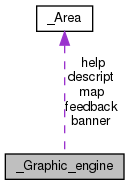
\includegraphics[width=169pt]{struct__Graphic__engine__coll__graph}
\end{center}
\end{figure}
\subsection*{Public Attributes}
\begin{DoxyCompactItemize}
\item 
\hyperlink{screen_8h_acfdfc42f6522d75fa3c16713afde8127}{Area} $\ast$ \hyperlink{struct__Graphic__engine_a1ea06bb881d335da8c31d63b3e834bdb}{map}
\item 
\hyperlink{screen_8h_acfdfc42f6522d75fa3c16713afde8127}{Area} $\ast$ \hyperlink{struct__Graphic__engine_a414bb888ecce3389c7ce348264758e58}{descript}
\item 
\hyperlink{screen_8h_acfdfc42f6522d75fa3c16713afde8127}{Area} $\ast$ \hyperlink{struct__Graphic__engine_a440dfb2c23c3c4b7d3871187371117b9}{banner}
\item 
\hyperlink{screen_8h_acfdfc42f6522d75fa3c16713afde8127}{Area} $\ast$ \hyperlink{struct__Graphic__engine_ade1d3e95ad6def427f613a4a2d101875}{help}
\item 
\hyperlink{screen_8h_acfdfc42f6522d75fa3c16713afde8127}{Area} $\ast$ \hyperlink{struct__Graphic__engine_a4fc0ef353d000b20d57fb75d898c6d2d}{feedback}
\end{DoxyCompactItemize}


\subsection{Detailed Description}
Estructura de la interfaz gráfica 

\subsection{Member Data Documentation}
\mbox{\Hypertarget{struct__Graphic__engine_a440dfb2c23c3c4b7d3871187371117b9}\label{struct__Graphic__engine_a440dfb2c23c3c4b7d3871187371117b9}} 
\index{\+\_\+\+Graphic\+\_\+engine@{\+\_\+\+Graphic\+\_\+engine}!banner@{banner}}
\index{banner@{banner}!\+\_\+\+Graphic\+\_\+engine@{\+\_\+\+Graphic\+\_\+engine}}
\subsubsection{\texorpdfstring{banner}{banner}}
{\footnotesize\ttfamily \hyperlink{screen_8h_acfdfc42f6522d75fa3c16713afde8127}{Area}$\ast$ \+\_\+\+Graphic\+\_\+engine\+::banner}

banner \mbox{\Hypertarget{struct__Graphic__engine_a414bb888ecce3389c7ce348264758e58}\label{struct__Graphic__engine_a414bb888ecce3389c7ce348264758e58}} 
\index{\+\_\+\+Graphic\+\_\+engine@{\+\_\+\+Graphic\+\_\+engine}!descript@{descript}}
\index{descript@{descript}!\+\_\+\+Graphic\+\_\+engine@{\+\_\+\+Graphic\+\_\+engine}}
\subsubsection{\texorpdfstring{descript}{descript}}
{\footnotesize\ttfamily \hyperlink{screen_8h_acfdfc42f6522d75fa3c16713afde8127}{Area}$\ast$ \+\_\+\+Graphic\+\_\+engine\+::descript}

descripcion \mbox{\Hypertarget{struct__Graphic__engine_a4fc0ef353d000b20d57fb75d898c6d2d}\label{struct__Graphic__engine_a4fc0ef353d000b20d57fb75d898c6d2d}} 
\index{\+\_\+\+Graphic\+\_\+engine@{\+\_\+\+Graphic\+\_\+engine}!feedback@{feedback}}
\index{feedback@{feedback}!\+\_\+\+Graphic\+\_\+engine@{\+\_\+\+Graphic\+\_\+engine}}
\subsubsection{\texorpdfstring{feedback}{feedback}}
{\footnotesize\ttfamily \hyperlink{screen_8h_acfdfc42f6522d75fa3c16713afde8127}{Area}$\ast$ \+\_\+\+Graphic\+\_\+engine\+::feedback}

Devuelve \mbox{\Hypertarget{struct__Graphic__engine_ade1d3e95ad6def427f613a4a2d101875}\label{struct__Graphic__engine_ade1d3e95ad6def427f613a4a2d101875}} 
\index{\+\_\+\+Graphic\+\_\+engine@{\+\_\+\+Graphic\+\_\+engine}!help@{help}}
\index{help@{help}!\+\_\+\+Graphic\+\_\+engine@{\+\_\+\+Graphic\+\_\+engine}}
\subsubsection{\texorpdfstring{help}{help}}
{\footnotesize\ttfamily \hyperlink{screen_8h_acfdfc42f6522d75fa3c16713afde8127}{Area}$\ast$ \+\_\+\+Graphic\+\_\+engine\+::help}

ayuda \mbox{\Hypertarget{struct__Graphic__engine_a1ea06bb881d335da8c31d63b3e834bdb}\label{struct__Graphic__engine_a1ea06bb881d335da8c31d63b3e834bdb}} 
\index{\+\_\+\+Graphic\+\_\+engine@{\+\_\+\+Graphic\+\_\+engine}!map@{map}}
\index{map@{map}!\+\_\+\+Graphic\+\_\+engine@{\+\_\+\+Graphic\+\_\+engine}}
\subsubsection{\texorpdfstring{map}{map}}
{\footnotesize\ttfamily \hyperlink{screen_8h_acfdfc42f6522d75fa3c16713afde8127}{Area}$\ast$ \+\_\+\+Graphic\+\_\+engine\+::map}

mapa 

The documentation for this struct was generated from the following file\+:\begin{DoxyCompactItemize}
\item 
\hyperlink{graphic__engine_8c}{graphic\+\_\+engine.\+c}\end{DoxyCompactItemize}

\hypertarget{struct__Inventory}{}\section{\+\_\+\+Inventory Struct Reference}
\label{struct__Inventory}\index{\+\_\+\+Inventory@{\+\_\+\+Inventory}}


Collaboration diagram for \+\_\+\+Inventory\+:
% FIG 0
\subsection*{Public Attributes}
\begin{DoxyCompactItemize}
\item 
\hyperlink{set_8h_a6d3b7f7c92cbb4577ef3ef7ddbf93161}{Set} $\ast$ \hyperlink{struct__Inventory_a478e4b50a62b9e7d5b17e335319faa97}{objects}
\item 
int \hyperlink{struct__Inventory_ae6dad9356e59d5e9ce48b09861be1516}{tam}
\end{DoxyCompactItemize}


\subsection{Detailed Description}
Estructura del inventario 

\subsection{Member Data Documentation}
\mbox{\Hypertarget{struct__Inventory_a478e4b50a62b9e7d5b17e335319faa97}\label{struct__Inventory_a478e4b50a62b9e7d5b17e335319faa97}} 
\index{\+\_\+\+Inventory@{\+\_\+\+Inventory}!objects@{objects}}
\index{objects@{objects}!\+\_\+\+Inventory@{\+\_\+\+Inventory}}
\subsubsection{\texorpdfstring{objects}{objects}}
{\footnotesize\ttfamily \hyperlink{set_8h_a6d3b7f7c92cbb4577ef3ef7ddbf93161}{Set}$\ast$ \+\_\+\+Inventory\+::objects}

objetos del inventario \mbox{\Hypertarget{struct__Inventory_ae6dad9356e59d5e9ce48b09861be1516}\label{struct__Inventory_ae6dad9356e59d5e9ce48b09861be1516}} 
\index{\+\_\+\+Inventory@{\+\_\+\+Inventory}!tam@{tam}}
\index{tam@{tam}!\+\_\+\+Inventory@{\+\_\+\+Inventory}}
\subsubsection{\texorpdfstring{tam}{tam}}
{\footnotesize\ttfamily int \+\_\+\+Inventory\+::tam}

tamaño maximo del inventario 

The documentation for this struct was generated from the following file\+:\begin{DoxyCompactItemize}
\item 
src/\hyperlink{inventory_8c}{inventory.\+c}\end{DoxyCompactItemize}

\hypertarget{struct__Link}{}\section{\+\_\+\+Link Struct Reference}
\label{struct__Link}\index{\+\_\+\+Link@{\+\_\+\+Link}}
\subsection*{Public Attributes}
\begin{DoxyCompactItemize}
\item 
\hyperlink{types_8h_a845e604fb28f7e3d97549da3448149d3}{Id} \hyperlink{struct__Link_a151212e7a8e8274c2a1ee991ba95878b}{id}
\item 
char \hyperlink{struct__Link_a5d81b67643f9c41056d8b199adbed77d}{name} \mbox{[}\hyperlink{types_8h_ae0b4816fb45161ef9da5e6d6134ee28a}{T\+AM}\mbox{]}
\item 
\hyperlink{types_8h_a845e604fb28f7e3d97549da3448149d3}{Id} \hyperlink{struct__Link_a9ea47d0c17026ae0e038fca89cd6fb7b}{id\+\_\+conexion} \mbox{[}2\mbox{]}
\item 
\hyperlink{types_8h_a3e5b8192e7d9ffaf3542f1210aec18dd}{B\+O\+OL} \hyperlink{struct__Link_a82cc94a1764a428c2eaaa6ef60fb3949}{state}
\end{DoxyCompactItemize}


\subsection{Detailed Description}
Estructura de link 

\subsection{Member Data Documentation}
\mbox{\Hypertarget{struct__Link_a151212e7a8e8274c2a1ee991ba95878b}\label{struct__Link_a151212e7a8e8274c2a1ee991ba95878b}} 
\index{\+\_\+\+Link@{\+\_\+\+Link}!id@{id}}
\index{id@{id}!\+\_\+\+Link@{\+\_\+\+Link}}
\subsubsection{\texorpdfstring{id}{id}}
{\footnotesize\ttfamily \hyperlink{types_8h_a845e604fb28f7e3d97549da3448149d3}{Id} \+\_\+\+Link\+::id}

Id del link \mbox{\Hypertarget{struct__Link_a9ea47d0c17026ae0e038fca89cd6fb7b}\label{struct__Link_a9ea47d0c17026ae0e038fca89cd6fb7b}} 
\index{\+\_\+\+Link@{\+\_\+\+Link}!id\+\_\+conexion@{id\+\_\+conexion}}
\index{id\+\_\+conexion@{id\+\_\+conexion}!\+\_\+\+Link@{\+\_\+\+Link}}
\subsubsection{\texorpdfstring{id\+\_\+conexion}{id\_conexion}}
{\footnotesize\ttfamily \hyperlink{types_8h_a845e604fb28f7e3d97549da3448149d3}{Id} \+\_\+\+Link\+::id\+\_\+conexion\mbox{[}2\mbox{]}}

Conexiones del likn \mbox{\Hypertarget{struct__Link_a5d81b67643f9c41056d8b199adbed77d}\label{struct__Link_a5d81b67643f9c41056d8b199adbed77d}} 
\index{\+\_\+\+Link@{\+\_\+\+Link}!name@{name}}
\index{name@{name}!\+\_\+\+Link@{\+\_\+\+Link}}
\subsubsection{\texorpdfstring{name}{name}}
{\footnotesize\ttfamily char \+\_\+\+Link\+::name\mbox{[}\hyperlink{types_8h_ae0b4816fb45161ef9da5e6d6134ee28a}{T\+AM}\mbox{]}}

Nombre \mbox{\Hypertarget{struct__Link_a82cc94a1764a428c2eaaa6ef60fb3949}\label{struct__Link_a82cc94a1764a428c2eaaa6ef60fb3949}} 
\index{\+\_\+\+Link@{\+\_\+\+Link}!state@{state}}
\index{state@{state}!\+\_\+\+Link@{\+\_\+\+Link}}
\subsubsection{\texorpdfstring{state}{state}}
{\footnotesize\ttfamily \hyperlink{types_8h_a3e5b8192e7d9ffaf3542f1210aec18dd}{B\+O\+OL} \+\_\+\+Link\+::state}

Estado\+: abierto o cerrado 

The documentation for this struct was generated from the following file\+:\begin{DoxyCompactItemize}
\item 
\hyperlink{link_8c}{link.\+c}\end{DoxyCompactItemize}

\hypertarget{struct__Object}{}\section{\+\_\+\+Object Struct Reference}
\label{struct__Object}\index{\+\_\+\+Object@{\+\_\+\+Object}}
\subsection*{Public Attributes}
\begin{DoxyCompactItemize}
\item 
\hyperlink{types_8h_a845e604fb28f7e3d97549da3448149d3}{Id} \hyperlink{struct__Object_a3cff7a0e8dc4e9d23895ed9af1b7653a}{id}
\item 
char \hyperlink{struct__Object_a3dab853826b88558a2c07dec50b96d57}{name} \mbox{[}\hyperlink{types_8h_a92ed8507d1cd2331ad09275c5c4c1c89}{W\+O\+R\+D\+\_\+\+S\+I\+ZE}\mbox{]}
\item 
char \hyperlink{struct__Object_a556e2e37c1461bcaae6492d2101f407d}{description} \mbox{[}\hyperlink{types_8h_a92ed8507d1cd2331ad09275c5c4c1c89}{W\+O\+R\+D\+\_\+\+S\+I\+ZE}\mbox{]}
\end{DoxyCompactItemize}


\subsection{Detailed Description}
Estructura del objeto 

\subsection{Member Data Documentation}
\mbox{\Hypertarget{struct__Object_a556e2e37c1461bcaae6492d2101f407d}\label{struct__Object_a556e2e37c1461bcaae6492d2101f407d}} 
\index{\+\_\+\+Object@{\+\_\+\+Object}!description@{description}}
\index{description@{description}!\+\_\+\+Object@{\+\_\+\+Object}}
\subsubsection{\texorpdfstring{description}{description}}
{\footnotesize\ttfamily char \+\_\+\+Object\+::description\mbox{[}\hyperlink{types_8h_a92ed8507d1cd2331ad09275c5c4c1c89}{W\+O\+R\+D\+\_\+\+S\+I\+ZE}\mbox{]}}

Descripcion del objeto \mbox{\Hypertarget{struct__Object_a3cff7a0e8dc4e9d23895ed9af1b7653a}\label{struct__Object_a3cff7a0e8dc4e9d23895ed9af1b7653a}} 
\index{\+\_\+\+Object@{\+\_\+\+Object}!id@{id}}
\index{id@{id}!\+\_\+\+Object@{\+\_\+\+Object}}
\subsubsection{\texorpdfstring{id}{id}}
{\footnotesize\ttfamily \hyperlink{types_8h_a845e604fb28f7e3d97549da3448149d3}{Id} \+\_\+\+Object\+::id}

Identificador del objeto \mbox{\Hypertarget{struct__Object_a3dab853826b88558a2c07dec50b96d57}\label{struct__Object_a3dab853826b88558a2c07dec50b96d57}} 
\index{\+\_\+\+Object@{\+\_\+\+Object}!name@{name}}
\index{name@{name}!\+\_\+\+Object@{\+\_\+\+Object}}
\subsubsection{\texorpdfstring{name}{name}}
{\footnotesize\ttfamily char \+\_\+\+Object\+::name\mbox{[}\hyperlink{types_8h_a92ed8507d1cd2331ad09275c5c4c1c89}{W\+O\+R\+D\+\_\+\+S\+I\+ZE}\mbox{]}}

Nombre del objeto 

The documentation for this struct was generated from the following file\+:\begin{DoxyCompactItemize}
\item 
\hyperlink{object_8c}{object.\+c}\end{DoxyCompactItemize}

\hypertarget{struct__Player}{}\section{\+\_\+\+Player Struct Reference}
\label{struct__Player}\index{\+\_\+\+Player@{\+\_\+\+Player}}


Collaboration diagram for \+\_\+\+Player\+:\nopagebreak
\begin{figure}[H]
\begin{center}
\leavevmode
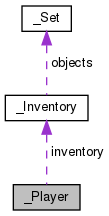
\includegraphics[width=154pt]{struct__Player__coll__graph}
\end{center}
\end{figure}
\subsection*{Public Attributes}
\begin{DoxyCompactItemize}
\item 
char \hyperlink{struct__Player_adda99df91c28eb58d392f2b43fc6898f}{name} \mbox{[}\hyperlink{types_8h_a92ed8507d1cd2331ad09275c5c4c1c89}{W\+O\+R\+D\+\_\+\+S\+I\+ZE}\mbox{]}
\item 
\hyperlink{types_8h_a845e604fb28f7e3d97549da3448149d3}{Id} \hyperlink{struct__Player_a60d635cd063816a9c1bd873f4868bb90}{id}
\item 
\hyperlink{inventory_8h_a2253bf64ac4ce6a9c1d6f39c0b0d32a3}{Inventory} $\ast$ \hyperlink{struct__Player_a5e02924cb82ca61f74ba414d190aa29b}{inventory}
\item 
\hyperlink{types_8h_a845e604fb28f7e3d97549da3448149d3}{Id} \hyperlink{struct__Player_aed09e7001b0005d679224be84e98d2a8}{space\+\_\+id}
\end{DoxyCompactItemize}


\subsection{Detailed Description}
Estructura del jugador 

\subsection{Member Data Documentation}
\mbox{\Hypertarget{struct__Player_a60d635cd063816a9c1bd873f4868bb90}\label{struct__Player_a60d635cd063816a9c1bd873f4868bb90}} 
\index{\+\_\+\+Player@{\+\_\+\+Player}!id@{id}}
\index{id@{id}!\+\_\+\+Player@{\+\_\+\+Player}}
\subsubsection{\texorpdfstring{id}{id}}
{\footnotesize\ttfamily \hyperlink{types_8h_a845e604fb28f7e3d97549da3448149d3}{Id} \+\_\+\+Player\+::id}

Su Id \mbox{\Hypertarget{struct__Player_a5e02924cb82ca61f74ba414d190aa29b}\label{struct__Player_a5e02924cb82ca61f74ba414d190aa29b}} 
\index{\+\_\+\+Player@{\+\_\+\+Player}!inventory@{inventory}}
\index{inventory@{inventory}!\+\_\+\+Player@{\+\_\+\+Player}}
\subsubsection{\texorpdfstring{inventory}{inventory}}
{\footnotesize\ttfamily \hyperlink{inventory_8h_a2253bf64ac4ce6a9c1d6f39c0b0d32a3}{Inventory}$\ast$ \+\_\+\+Player\+::inventory}

El inventario del jugador \mbox{\Hypertarget{struct__Player_adda99df91c28eb58d392f2b43fc6898f}\label{struct__Player_adda99df91c28eb58d392f2b43fc6898f}} 
\index{\+\_\+\+Player@{\+\_\+\+Player}!name@{name}}
\index{name@{name}!\+\_\+\+Player@{\+\_\+\+Player}}
\subsubsection{\texorpdfstring{name}{name}}
{\footnotesize\ttfamily char \+\_\+\+Player\+::name\mbox{[}\hyperlink{types_8h_a92ed8507d1cd2331ad09275c5c4c1c89}{W\+O\+R\+D\+\_\+\+S\+I\+ZE}\mbox{]}}

Nombre del jugador \mbox{\Hypertarget{struct__Player_aed09e7001b0005d679224be84e98d2a8}\label{struct__Player_aed09e7001b0005d679224be84e98d2a8}} 
\index{\+\_\+\+Player@{\+\_\+\+Player}!space\+\_\+id@{space\+\_\+id}}
\index{space\+\_\+id@{space\+\_\+id}!\+\_\+\+Player@{\+\_\+\+Player}}
\subsubsection{\texorpdfstring{space\+\_\+id}{space\_id}}
{\footnotesize\ttfamily \hyperlink{types_8h_a845e604fb28f7e3d97549da3448149d3}{Id} \+\_\+\+Player\+::space\+\_\+id}

El número identificador del espacio en el que se encuentra el jugador 

The documentation for this struct was generated from the following file\+:\begin{DoxyCompactItemize}
\item 
\hyperlink{player_8c}{player.\+c}\end{DoxyCompactItemize}

\hypertarget{struct__Set}{}\section{\+\_\+\+Set Struct Reference}
\label{struct__Set}\index{\+\_\+\+Set@{\+\_\+\+Set}}
\subsection*{Public Attributes}
\begin{DoxyCompactItemize}
\item 
\hyperlink{types_8h_a845e604fb28f7e3d97549da3448149d3}{Id} \hyperlink{struct__Set_aaa814a92620bfdb539ed25be204a3079}{id} \mbox{[}\hyperlink{set_8h_a24b51e1a036e3b382adcc8216239aafd}{T\+A\+M\+\_\+\+S\+ET}\mbox{]}
\item 
int \hyperlink{struct__Set_a6d4c5bc1c085564602a0e93fe074ad91}{num\+\_\+obj}
\end{DoxyCompactItemize}


\subsection{Detailed Description}
Estructura de Set 

\subsection{Member Data Documentation}
\mbox{\Hypertarget{struct__Set_aaa814a92620bfdb539ed25be204a3079}\label{struct__Set_aaa814a92620bfdb539ed25be204a3079}} 
\index{\+\_\+\+Set@{\+\_\+\+Set}!id@{id}}
\index{id@{id}!\+\_\+\+Set@{\+\_\+\+Set}}
\subsubsection{\texorpdfstring{id}{id}}
{\footnotesize\ttfamily \hyperlink{types_8h_a845e604fb28f7e3d97549da3448149d3}{Id} \+\_\+\+Set\+::id\mbox{[}\hyperlink{set_8h_a24b51e1a036e3b382adcc8216239aafd}{T\+A\+M\+\_\+\+S\+ET}\mbox{]}}

ids \mbox{\Hypertarget{struct__Set_a6d4c5bc1c085564602a0e93fe074ad91}\label{struct__Set_a6d4c5bc1c085564602a0e93fe074ad91}} 
\index{\+\_\+\+Set@{\+\_\+\+Set}!num\+\_\+obj@{num\+\_\+obj}}
\index{num\+\_\+obj@{num\+\_\+obj}!\+\_\+\+Set@{\+\_\+\+Set}}
\subsubsection{\texorpdfstring{num\+\_\+obj}{num\_obj}}
{\footnotesize\ttfamily int \+\_\+\+Set\+::num\+\_\+obj}

numero de ids almacenados 

The documentation for this struct was generated from the following file\+:\begin{DoxyCompactItemize}
\item 
src/\hyperlink{set_8c}{set.\+c}\end{DoxyCompactItemize}

\hypertarget{struct__Space}{}\section{\+\_\+\+Space Struct Reference}
\label{struct__Space}\index{\+\_\+\+Space@{\+\_\+\+Space}}


Collaboration diagram for \+\_\+\+Space\+:
% FIG 0
\subsection*{Public Attributes}
\begin{DoxyCompactItemize}
\item 
\hyperlink{types_8h_a845e604fb28f7e3d97549da3448149d3}{Id} \hyperlink{struct__Space_a70cb461deb9ac073e401b607339b567f}{id}
\item 
char \hyperlink{struct__Space_aa1c9c994c2d16ecf3ef46138685fdfdc}{name} \mbox{[}\hyperlink{types_8h_a92ed8507d1cd2331ad09275c5c4c1c89}{W\+O\+R\+D\+\_\+\+S\+I\+ZE}+1\mbox{]}
\item 
\hyperlink{types_8h_a845e604fb28f7e3d97549da3448149d3}{Id} \hyperlink{struct__Space_ae5ebe53ce79514d7d2d93911e0159252}{north}
\item 
\hyperlink{types_8h_a845e604fb28f7e3d97549da3448149d3}{Id} \hyperlink{struct__Space_a646b68c22a0bbf1685033c96109d31d1}{south}
\item 
\hyperlink{types_8h_a845e604fb28f7e3d97549da3448149d3}{Id} \hyperlink{struct__Space_a41ce2bf33cf0c157b358221f094ee05b}{east}
\item 
\hyperlink{types_8h_a845e604fb28f7e3d97549da3448149d3}{Id} \hyperlink{struct__Space_a20c1d259e93b44e24ba82982e142eb9b}{west}
\item 
\hyperlink{types_8h_a845e604fb28f7e3d97549da3448149d3}{Id} \hyperlink{struct__Space_af2a50145d93dfb8d82b8b42138dc57a1}{up}
\item 
\hyperlink{types_8h_a845e604fb28f7e3d97549da3448149d3}{Id} \hyperlink{struct__Space_ac20194f418676bb03cca7e0fdcb6f559}{down}
\item 
\hyperlink{set_8h_a6d3b7f7c92cbb4577ef3ef7ddbf93161}{Set} $\ast$ \hyperlink{struct__Space_a661ed8b0fc8085b6db70188aa5085625}{objects}
\item 
char \hyperlink{struct__Space_af311939768f2208925e07a50ebd3f045}{gdesc} \mbox{[}\hyperlink{space_8h_a894ebc9b2098fe63607e0ca2e5f5ce8d}{T\+A\+M\+\_\+\+D\+I\+B\+U\+JO}+1\mbox{]}
\item 
char \hyperlink{struct__Space_a2a50aacb78d1d0f65f5b14f94ed81d80}{description} \mbox{[}\hyperlink{types_8h_a92ed8507d1cd2331ad09275c5c4c1c89}{W\+O\+R\+D\+\_\+\+S\+I\+ZE}\mbox{]}
\item 
\hyperlink{types_8h_a3e5b8192e7d9ffaf3542f1210aec18dd}{B\+O\+OL} \hyperlink{struct__Space_a15f20d8ccdec846b9a4f77464748bff5}{light}
\item 
char \hyperlink{struct__Space_a5b0f12b84b11444282405bb6ae64f442}{detailed\+\_\+description} \mbox{[}\hyperlink{types_8h_a92ed8507d1cd2331ad09275c5c4c1c89}{W\+O\+R\+D\+\_\+\+S\+I\+ZE}\mbox{]}
\end{DoxyCompactItemize}


\subsection{Detailed Description}
Estructura de espacio 

\subsection{Member Data Documentation}
\mbox{\Hypertarget{struct__Space_a2a50aacb78d1d0f65f5b14f94ed81d80}\label{struct__Space_a2a50aacb78d1d0f65f5b14f94ed81d80}} 
\index{\+\_\+\+Space@{\+\_\+\+Space}!description@{description}}
\index{description@{description}!\+\_\+\+Space@{\+\_\+\+Space}}
\subsubsection{\texorpdfstring{description}{description}}
{\footnotesize\ttfamily char \+\_\+\+Space\+::description\mbox{[}\hyperlink{types_8h_a92ed8507d1cd2331ad09275c5c4c1c89}{W\+O\+R\+D\+\_\+\+S\+I\+ZE}\mbox{]}}

La descripcion del espacio \mbox{\Hypertarget{struct__Space_a5b0f12b84b11444282405bb6ae64f442}\label{struct__Space_a5b0f12b84b11444282405bb6ae64f442}} 
\index{\+\_\+\+Space@{\+\_\+\+Space}!detailed\+\_\+description@{detailed\+\_\+description}}
\index{detailed\+\_\+description@{detailed\+\_\+description}!\+\_\+\+Space@{\+\_\+\+Space}}
\subsubsection{\texorpdfstring{detailed\+\_\+description}{detailed\_description}}
{\footnotesize\ttfamily char \+\_\+\+Space\+::detailed\+\_\+description\mbox{[}\hyperlink{types_8h_a92ed8507d1cd2331ad09275c5c4c1c89}{W\+O\+R\+D\+\_\+\+S\+I\+ZE}\mbox{]}}

La descripcion detallada del espacio \mbox{\Hypertarget{struct__Space_ac20194f418676bb03cca7e0fdcb6f559}\label{struct__Space_ac20194f418676bb03cca7e0fdcb6f559}} 
\index{\+\_\+\+Space@{\+\_\+\+Space}!down@{down}}
\index{down@{down}!\+\_\+\+Space@{\+\_\+\+Space}}
\subsubsection{\texorpdfstring{down}{down}}
{\footnotesize\ttfamily \hyperlink{types_8h_a845e604fb28f7e3d97549da3448149d3}{Id} \+\_\+\+Space\+::down}

Id del espacio abajo \mbox{\Hypertarget{struct__Space_a41ce2bf33cf0c157b358221f094ee05b}\label{struct__Space_a41ce2bf33cf0c157b358221f094ee05b}} 
\index{\+\_\+\+Space@{\+\_\+\+Space}!east@{east}}
\index{east@{east}!\+\_\+\+Space@{\+\_\+\+Space}}
\subsubsection{\texorpdfstring{east}{east}}
{\footnotesize\ttfamily \hyperlink{types_8h_a845e604fb28f7e3d97549da3448149d3}{Id} \+\_\+\+Space\+::east}

Id del espacio al este \mbox{\Hypertarget{struct__Space_af311939768f2208925e07a50ebd3f045}\label{struct__Space_af311939768f2208925e07a50ebd3f045}} 
\index{\+\_\+\+Space@{\+\_\+\+Space}!gdesc@{gdesc}}
\index{gdesc@{gdesc}!\+\_\+\+Space@{\+\_\+\+Space}}
\subsubsection{\texorpdfstring{gdesc}{gdesc}}
{\footnotesize\ttfamily char \+\_\+\+Space\+::gdesc\mbox{[}\hyperlink{space_8h_a894ebc9b2098fe63607e0ca2e5f5ce8d}{T\+A\+M\+\_\+\+D\+I\+B\+U\+JO}+1\mbox{]}}

el dibujo \mbox{\Hypertarget{struct__Space_a70cb461deb9ac073e401b607339b567f}\label{struct__Space_a70cb461deb9ac073e401b607339b567f}} 
\index{\+\_\+\+Space@{\+\_\+\+Space}!id@{id}}
\index{id@{id}!\+\_\+\+Space@{\+\_\+\+Space}}
\subsubsection{\texorpdfstring{id}{id}}
{\footnotesize\ttfamily \hyperlink{types_8h_a845e604fb28f7e3d97549da3448149d3}{Id} \+\_\+\+Space\+::id}

Id del espacio \mbox{\Hypertarget{struct__Space_a15f20d8ccdec846b9a4f77464748bff5}\label{struct__Space_a15f20d8ccdec846b9a4f77464748bff5}} 
\index{\+\_\+\+Space@{\+\_\+\+Space}!light@{light}}
\index{light@{light}!\+\_\+\+Space@{\+\_\+\+Space}}
\subsubsection{\texorpdfstring{light}{light}}
{\footnotesize\ttfamily \hyperlink{types_8h_a3e5b8192e7d9ffaf3542f1210aec18dd}{B\+O\+OL} \+\_\+\+Space\+::light}

Iluminación del espacio \mbox{\Hypertarget{struct__Space_aa1c9c994c2d16ecf3ef46138685fdfdc}\label{struct__Space_aa1c9c994c2d16ecf3ef46138685fdfdc}} 
\index{\+\_\+\+Space@{\+\_\+\+Space}!name@{name}}
\index{name@{name}!\+\_\+\+Space@{\+\_\+\+Space}}
\subsubsection{\texorpdfstring{name}{name}}
{\footnotesize\ttfamily char \+\_\+\+Space\+::name\mbox{[}\hyperlink{types_8h_a92ed8507d1cd2331ad09275c5c4c1c89}{W\+O\+R\+D\+\_\+\+S\+I\+ZE}+1\mbox{]}}

Su nombre \mbox{\Hypertarget{struct__Space_ae5ebe53ce79514d7d2d93911e0159252}\label{struct__Space_ae5ebe53ce79514d7d2d93911e0159252}} 
\index{\+\_\+\+Space@{\+\_\+\+Space}!north@{north}}
\index{north@{north}!\+\_\+\+Space@{\+\_\+\+Space}}
\subsubsection{\texorpdfstring{north}{north}}
{\footnotesize\ttfamily \hyperlink{types_8h_a845e604fb28f7e3d97549da3448149d3}{Id} \+\_\+\+Space\+::north}

Id del espacio al norte \mbox{\Hypertarget{struct__Space_a661ed8b0fc8085b6db70188aa5085625}\label{struct__Space_a661ed8b0fc8085b6db70188aa5085625}} 
\index{\+\_\+\+Space@{\+\_\+\+Space}!objects@{objects}}
\index{objects@{objects}!\+\_\+\+Space@{\+\_\+\+Space}}
\subsubsection{\texorpdfstring{objects}{objects}}
{\footnotesize\ttfamily \hyperlink{set_8h_a6d3b7f7c92cbb4577ef3ef7ddbf93161}{Set}$\ast$ \+\_\+\+Space\+::objects}

Id de los objetos que contiene \mbox{\Hypertarget{struct__Space_a646b68c22a0bbf1685033c96109d31d1}\label{struct__Space_a646b68c22a0bbf1685033c96109d31d1}} 
\index{\+\_\+\+Space@{\+\_\+\+Space}!south@{south}}
\index{south@{south}!\+\_\+\+Space@{\+\_\+\+Space}}
\subsubsection{\texorpdfstring{south}{south}}
{\footnotesize\ttfamily \hyperlink{types_8h_a845e604fb28f7e3d97549da3448149d3}{Id} \+\_\+\+Space\+::south}

Id del espacio al sur \mbox{\Hypertarget{struct__Space_af2a50145d93dfb8d82b8b42138dc57a1}\label{struct__Space_af2a50145d93dfb8d82b8b42138dc57a1}} 
\index{\+\_\+\+Space@{\+\_\+\+Space}!up@{up}}
\index{up@{up}!\+\_\+\+Space@{\+\_\+\+Space}}
\subsubsection{\texorpdfstring{up}{up}}
{\footnotesize\ttfamily \hyperlink{types_8h_a845e604fb28f7e3d97549da3448149d3}{Id} \+\_\+\+Space\+::up}

Id del espacio arriba \mbox{\Hypertarget{struct__Space_a20c1d259e93b44e24ba82982e142eb9b}\label{struct__Space_a20c1d259e93b44e24ba82982e142eb9b}} 
\index{\+\_\+\+Space@{\+\_\+\+Space}!west@{west}}
\index{west@{west}!\+\_\+\+Space@{\+\_\+\+Space}}
\subsubsection{\texorpdfstring{west}{west}}
{\footnotesize\ttfamily \hyperlink{types_8h_a845e604fb28f7e3d97549da3448149d3}{Id} \+\_\+\+Space\+::west}

Id del espacio al oeste 

The documentation for this struct was generated from the following file\+:\begin{DoxyCompactItemize}
\item 
src/\hyperlink{space_8c}{space.\+c}\end{DoxyCompactItemize}

\chapter{File Documentation}
\hypertarget{command_8h}{}\section{command.\+h File Reference}
\label{command_8h}\index{command.\+h@{command.\+h}}


En este fichero definimos las funciones para los comandos.  


{\ttfamily \#include \char`\"{}types.\+h\char`\"{}}\newline
Include dependency graph for command.\+h\+:\nopagebreak
\begin{figure}[H]
\begin{center}
\leavevmode
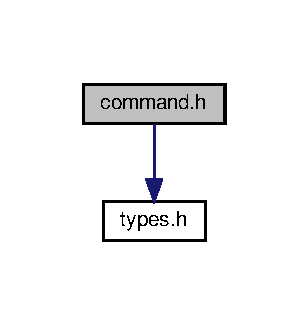
\includegraphics[width=148pt]{command_8h__incl}
\end{center}
\end{figure}
This graph shows which files directly or indirectly include this file\+:\nopagebreak
\begin{figure}[H]
\begin{center}
\leavevmode
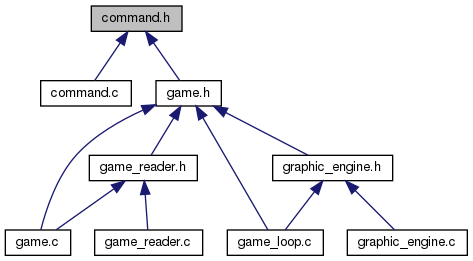
\includegraphics[width=350pt]{command_8h__dep__incl}
\end{center}
\end{figure}
\subsection*{Typedefs}
\begin{DoxyCompactItemize}
\item 
typedef enum \hyperlink{command_8h_ace19ba2296a74e4aef53304e0934c50c}{enum\+\_\+\+Command} \hyperlink{command_8h_a0473597db8c45c0289b6b8e2f8abbe32}{T\+\_\+\+Command}
\item 
typedef struct \hyperlink{struct__Comand}{\+\_\+\+Comand} \hyperlink{command_8h_a64fc5834e0580f5f7517e120bd31c301}{Comand}
\end{DoxyCompactItemize}
\subsection*{Enumerations}
\begin{DoxyCompactItemize}
\item 
enum \hyperlink{command_8h_ace19ba2296a74e4aef53304e0934c50c}{enum\+\_\+\+Command} \{ \newline
\hyperlink{command_8h_ace19ba2296a74e4aef53304e0934c50ca785693a1d550a18688638e9124af41d0}{N\+O\+\_\+\+C\+MD} = -\/1, 
\hyperlink{command_8h_ace19ba2296a74e4aef53304e0934c50ca6ce26a62afab55d7606ad4e92428b30c}{U\+N\+K\+N\+O\+WN}, 
\hyperlink{command_8h_ace19ba2296a74e4aef53304e0934c50ca76bdc8adfd6c6463ab269ff4c06be9b4}{Q\+U\+IT}, 
\hyperlink{command_8h_ace19ba2296a74e4aef53304e0934c50ca50d8e53aac4e002d0fd296c5033ce985}{GO}, 
\newline
\hyperlink{command_8h_ace19ba2296a74e4aef53304e0934c50ca7405647410e343caba1bf383e83d4f5f}{T\+A\+KE}, 
\hyperlink{command_8h_ace19ba2296a74e4aef53304e0934c50cae09e07839103de682cb13fa773793fc0}{L\+E\+A\+VE}, 
\hyperlink{command_8h_ace19ba2296a74e4aef53304e0934c50ca2eeb9fef8a6a516fa6437a44a6efbd52}{R\+O\+LL}, 
\hyperlink{command_8h_ace19ba2296a74e4aef53304e0934c50caab933f64fcaa285df294e1420f6f1b07}{I\+N\+S\+P\+E\+CT}, 
\newline
\hyperlink{command_8h_ace19ba2296a74e4aef53304e0934c50cac241aecbe2e3eba2f42ce28777f6ab65}{F\+O\+L\+L\+O\+W\+I\+NG}, 
\hyperlink{command_8h_ace19ba2296a74e4aef53304e0934c50cad9600a436d5cc272dfd53f6c45fdeca4}{P\+R\+E\+V\+I\+O\+US}, 
\hyperlink{command_8h_ace19ba2296a74e4aef53304e0934c50cac3988b12a039e31264513788c40ad322}{O\+C\+A\+\_\+\+F\+O\+L\+L\+O\+W\+I\+NG}, 
\hyperlink{command_8h_ace19ba2296a74e4aef53304e0934c50ca356a23a6d4264f3ba8a5dc3f5a1fa640}{O\+C\+A\+\_\+\+P\+R\+E\+V\+I\+O\+US}
 \}
\end{DoxyCompactItemize}
\subsection*{Functions}
\begin{DoxyCompactItemize}
\item 
\hyperlink{types_8h_a32c27cc471df37f4fc818d65de0a56c4}{S\+T\+A\+T\+US} \hyperlink{command_8h_ab73f9b21268fcb7c4d6918aae58738e7}{comand\+\_\+get\+\_\+user\+\_\+input} (\hyperlink{command_8h_a64fc5834e0580f5f7517e120bd31c301}{Comand} $\ast$comand)
\begin{DoxyCompactList}\small\item\em lee el comando del teclado y si es valido lo ejecuta \end{DoxyCompactList}\item 
\hyperlink{command_8h_a64fc5834e0580f5f7517e120bd31c301}{Comand} $\ast$ \hyperlink{command_8h_aca59ac581052c5503087f1a29b77f8ca}{comand\+\_\+create} ()
\begin{DoxyCompactList}\small\item\em crea un comando definiendo sus campos como U\+N\+K\+N\+O\+WN \end{DoxyCompactList}\item 
void \hyperlink{command_8h_a266fc377d9fa9c814084e4507b006e70}{comand\+\_\+destroy} (\hyperlink{command_8h_a64fc5834e0580f5f7517e120bd31c301}{Comand} $\ast$comand)
\begin{DoxyCompactList}\small\item\em destruye el comando y libera la memoria \end{DoxyCompactList}\item 
\hyperlink{command_8h_a0473597db8c45c0289b6b8e2f8abbe32}{T\+\_\+\+Command} \hyperlink{command_8h_a37c537079e0f082c79bd4a576a8b81d0}{comand\+\_\+get\+\_\+comand} (\hyperlink{command_8h_a64fc5834e0580f5f7517e120bd31c301}{Comand} $\ast$comand)
\begin{DoxyCompactList}\small\item\em devuelve el simbolo del comando que se le pasa \end{DoxyCompactList}\item 
char $\ast$ \hyperlink{command_8h_ab8f45898e8b760f47f7c6a34f1102e6e}{comand\+\_\+get\+\_\+name} (\hyperlink{command_8h_a64fc5834e0580f5f7517e120bd31c301}{Comand} $\ast$comand)
\begin{DoxyCompactList}\small\item\em devuelve el nombre del comando que se le pasa \end{DoxyCompactList}\end{DoxyCompactItemize}


\subsection{Detailed Description}
En este fichero definimos las funciones para los comandos. 

\begin{DoxyAuthor}{Author}
Manuel Suarez, Saul Almazán, Álvaro Becerra, Rodrigo Lardiés 
\end{DoxyAuthor}
\begin{DoxyVersion}{Version}
3.\+0 
\end{DoxyVersion}
\begin{DoxyDate}{Date}
7/10/2018 
\end{DoxyDate}


\subsection{Typedef Documentation}
\mbox{\Hypertarget{command_8h_a64fc5834e0580f5f7517e120bd31c301}\label{command_8h_a64fc5834e0580f5f7517e120bd31c301}} 
\index{command.\+h@{command.\+h}!Comand@{Comand}}
\index{Comand@{Comand}!command.\+h@{command.\+h}}
\subsubsection{\texorpdfstring{Comand}{Comand}}
{\footnotesize\ttfamily typedef struct \hyperlink{struct__Comand}{\+\_\+\+Comand} \hyperlink{command_8h_a64fc5834e0580f5f7517e120bd31c301}{Comand}}

definicion de la estructura de comando \mbox{\Hypertarget{command_8h_a0473597db8c45c0289b6b8e2f8abbe32}\label{command_8h_a0473597db8c45c0289b6b8e2f8abbe32}} 
\index{command.\+h@{command.\+h}!T\+\_\+\+Command@{T\+\_\+\+Command}}
\index{T\+\_\+\+Command@{T\+\_\+\+Command}!command.\+h@{command.\+h}}
\subsubsection{\texorpdfstring{T\+\_\+\+Command}{T\_Command}}
{\footnotesize\ttfamily typedef enum \hyperlink{command_8h_ace19ba2296a74e4aef53304e0934c50c}{enum\+\_\+\+Command}  \hyperlink{command_8h_a0473597db8c45c0289b6b8e2f8abbe32}{T\+\_\+\+Command}}

Enumeracion de posibles comandos\+Posibles comandos 

\subsection{Enumeration Type Documentation}
\mbox{\Hypertarget{command_8h_ace19ba2296a74e4aef53304e0934c50c}\label{command_8h_ace19ba2296a74e4aef53304e0934c50c}} 
\index{command.\+h@{command.\+h}!enum\+\_\+\+Command@{enum\+\_\+\+Command}}
\index{enum\+\_\+\+Command@{enum\+\_\+\+Command}!command.\+h@{command.\+h}}
\subsubsection{\texorpdfstring{enum\+\_\+\+Command}{enum\_Command}}
{\footnotesize\ttfamily enum \hyperlink{command_8h_ace19ba2296a74e4aef53304e0934c50c}{enum\+\_\+\+Command}}

Enumeracion de posibles comandos \begin{DoxyEnumFields}{Enumerator}
\raisebox{\heightof{T}}[0pt][0pt]{\index{N\+O\+\_\+\+C\+MD@{N\+O\+\_\+\+C\+MD}!command.\+h@{command.\+h}}\index{command.\+h@{command.\+h}!N\+O\+\_\+\+C\+MD@{N\+O\+\_\+\+C\+MD}}}\mbox{\Hypertarget{command_8h_ace19ba2296a74e4aef53304e0934c50ca785693a1d550a18688638e9124af41d0}\label{command_8h_ace19ba2296a74e4aef53304e0934c50ca785693a1d550a18688638e9124af41d0}} 
N\+O\+\_\+\+C\+MD&Sin comando \\
\hline

\raisebox{\heightof{T}}[0pt][0pt]{\index{U\+N\+K\+N\+O\+WN@{U\+N\+K\+N\+O\+WN}!command.\+h@{command.\+h}}\index{command.\+h@{command.\+h}!U\+N\+K\+N\+O\+WN@{U\+N\+K\+N\+O\+WN}}}\mbox{\Hypertarget{command_8h_ace19ba2296a74e4aef53304e0934c50ca6ce26a62afab55d7606ad4e92428b30c}\label{command_8h_ace19ba2296a74e4aef53304e0934c50ca6ce26a62afab55d7606ad4e92428b30c}} 
U\+N\+K\+N\+O\+WN&Desconocido \\
\hline

\raisebox{\heightof{T}}[0pt][0pt]{\index{Q\+U\+IT@{Q\+U\+IT}!command.\+h@{command.\+h}}\index{command.\+h@{command.\+h}!Q\+U\+IT@{Q\+U\+IT}}}\mbox{\Hypertarget{command_8h_ace19ba2296a74e4aef53304e0934c50ca76bdc8adfd6c6463ab269ff4c06be9b4}\label{command_8h_ace19ba2296a74e4aef53304e0934c50ca76bdc8adfd6c6463ab269ff4c06be9b4}} 
Q\+U\+IT&Salir \\
\hline

\raisebox{\heightof{T}}[0pt][0pt]{\index{GO@{GO}!command.\+h@{command.\+h}}\index{command.\+h@{command.\+h}!GO@{GO}}}\mbox{\Hypertarget{command_8h_ace19ba2296a74e4aef53304e0934c50ca50d8e53aac4e002d0fd296c5033ce985}\label{command_8h_ace19ba2296a74e4aef53304e0934c50ca50d8e53aac4e002d0fd296c5033ce985}} 
GO&Seguir \\
\hline

\raisebox{\heightof{T}}[0pt][0pt]{\index{T\+A\+KE@{T\+A\+KE}!command.\+h@{command.\+h}}\index{command.\+h@{command.\+h}!T\+A\+KE@{T\+A\+KE}}}\mbox{\Hypertarget{command_8h_ace19ba2296a74e4aef53304e0934c50ca7405647410e343caba1bf383e83d4f5f}\label{command_8h_ace19ba2296a74e4aef53304e0934c50ca7405647410e343caba1bf383e83d4f5f}} 
T\+A\+KE&Coger objeto \\
\hline

\raisebox{\heightof{T}}[0pt][0pt]{\index{L\+E\+A\+VE@{L\+E\+A\+VE}!command.\+h@{command.\+h}}\index{command.\+h@{command.\+h}!L\+E\+A\+VE@{L\+E\+A\+VE}}}\mbox{\Hypertarget{command_8h_ace19ba2296a74e4aef53304e0934c50cae09e07839103de682cb13fa773793fc0}\label{command_8h_ace19ba2296a74e4aef53304e0934c50cae09e07839103de682cb13fa773793fc0}} 
L\+E\+A\+VE&Soltar objeto \\
\hline

\raisebox{\heightof{T}}[0pt][0pt]{\index{R\+O\+LL@{R\+O\+LL}!command.\+h@{command.\+h}}\index{command.\+h@{command.\+h}!R\+O\+LL@{R\+O\+LL}}}\mbox{\Hypertarget{command_8h_ace19ba2296a74e4aef53304e0934c50ca2eeb9fef8a6a516fa6437a44a6efbd52}\label{command_8h_ace19ba2296a74e4aef53304e0934c50ca2eeb9fef8a6a516fa6437a44a6efbd52}} 
R\+O\+LL&Tirar el dado \\
\hline

\raisebox{\heightof{T}}[0pt][0pt]{\index{I\+N\+S\+P\+E\+CT@{I\+N\+S\+P\+E\+CT}!command.\+h@{command.\+h}}\index{command.\+h@{command.\+h}!I\+N\+S\+P\+E\+CT@{I\+N\+S\+P\+E\+CT}}}\mbox{\Hypertarget{command_8h_ace19ba2296a74e4aef53304e0934c50caab933f64fcaa285df294e1420f6f1b07}\label{command_8h_ace19ba2296a74e4aef53304e0934c50caab933f64fcaa285df294e1420f6f1b07}} 
I\+N\+S\+P\+E\+CT&Inspeccionar \\
\hline

\raisebox{\heightof{T}}[0pt][0pt]{\index{F\+O\+L\+L\+O\+W\+I\+NG@{F\+O\+L\+L\+O\+W\+I\+NG}!command.\+h@{command.\+h}}\index{command.\+h@{command.\+h}!F\+O\+L\+L\+O\+W\+I\+NG@{F\+O\+L\+L\+O\+W\+I\+NG}}}\mbox{\Hypertarget{command_8h_ace19ba2296a74e4aef53304e0934c50cac241aecbe2e3eba2f42ce28777f6ab65}\label{command_8h_ace19ba2296a74e4aef53304e0934c50cac241aecbe2e3eba2f42ce28777f6ab65}} 
F\+O\+L\+L\+O\+W\+I\+NG&Siguiente \\
\hline

\raisebox{\heightof{T}}[0pt][0pt]{\index{P\+R\+E\+V\+I\+O\+US@{P\+R\+E\+V\+I\+O\+US}!command.\+h@{command.\+h}}\index{command.\+h@{command.\+h}!P\+R\+E\+V\+I\+O\+US@{P\+R\+E\+V\+I\+O\+US}}}\mbox{\Hypertarget{command_8h_ace19ba2296a74e4aef53304e0934c50cad9600a436d5cc272dfd53f6c45fdeca4}\label{command_8h_ace19ba2296a74e4aef53304e0934c50cad9600a436d5cc272dfd53f6c45fdeca4}} 
P\+R\+E\+V\+I\+O\+US&Anterior \\
\hline

\raisebox{\heightof{T}}[0pt][0pt]{\index{O\+C\+A\+\_\+\+F\+O\+L\+L\+O\+W\+I\+NG@{O\+C\+A\+\_\+\+F\+O\+L\+L\+O\+W\+I\+NG}!command.\+h@{command.\+h}}\index{command.\+h@{command.\+h}!O\+C\+A\+\_\+\+F\+O\+L\+L\+O\+W\+I\+NG@{O\+C\+A\+\_\+\+F\+O\+L\+L\+O\+W\+I\+NG}}}\mbox{\Hypertarget{command_8h_ace19ba2296a74e4aef53304e0934c50cac3988b12a039e31264513788c40ad322}\label{command_8h_ace19ba2296a74e4aef53304e0934c50cac3988b12a039e31264513788c40ad322}} 
O\+C\+A\+\_\+\+F\+O\+L\+L\+O\+W\+I\+NG&Oca siguiente \\
\hline

\raisebox{\heightof{T}}[0pt][0pt]{\index{O\+C\+A\+\_\+\+P\+R\+E\+V\+I\+O\+US@{O\+C\+A\+\_\+\+P\+R\+E\+V\+I\+O\+US}!command.\+h@{command.\+h}}\index{command.\+h@{command.\+h}!O\+C\+A\+\_\+\+P\+R\+E\+V\+I\+O\+US@{O\+C\+A\+\_\+\+P\+R\+E\+V\+I\+O\+US}}}\mbox{\Hypertarget{command_8h_ace19ba2296a74e4aef53304e0934c50ca356a23a6d4264f3ba8a5dc3f5a1fa640}\label{command_8h_ace19ba2296a74e4aef53304e0934c50ca356a23a6d4264f3ba8a5dc3f5a1fa640}} 
O\+C\+A\+\_\+\+P\+R\+E\+V\+I\+O\+US&Oca anterior \\
\hline

\end{DoxyEnumFields}


\subsection{Function Documentation}
\mbox{\Hypertarget{command_8h_aca59ac581052c5503087f1a29b77f8ca}\label{command_8h_aca59ac581052c5503087f1a29b77f8ca}} 
\index{command.\+h@{command.\+h}!comand\+\_\+create@{comand\+\_\+create}}
\index{comand\+\_\+create@{comand\+\_\+create}!command.\+h@{command.\+h}}
\subsubsection{\texorpdfstring{comand\+\_\+create()}{comand\_create()}}
{\footnotesize\ttfamily \hyperlink{command_8h_a64fc5834e0580f5f7517e120bd31c301}{Comand}$\ast$ comand\+\_\+create (\begin{DoxyParamCaption}{ }\end{DoxyParamCaption})}



crea un comando definiendo sus campos como U\+N\+K\+N\+O\+WN 

\begin{DoxyAuthor}{Author}
Manuel Suarez, Saul Almazán, Álvaro Becerra, Rodrigo Lardiés 
\end{DoxyAuthor}
\begin{DoxyDate}{Date}
10/11/2018 
\end{DoxyDate}
\begin{DoxyReturn}{Returns}
comand$\ast$ (el comando creado) 
\end{DoxyReturn}
\mbox{\Hypertarget{command_8h_a266fc377d9fa9c814084e4507b006e70}\label{command_8h_a266fc377d9fa9c814084e4507b006e70}} 
\index{command.\+h@{command.\+h}!comand\+\_\+destroy@{comand\+\_\+destroy}}
\index{comand\+\_\+destroy@{comand\+\_\+destroy}!command.\+h@{command.\+h}}
\subsubsection{\texorpdfstring{comand\+\_\+destroy()}{comand\_destroy()}}
{\footnotesize\ttfamily void comand\+\_\+destroy (\begin{DoxyParamCaption}\item[{\hyperlink{command_8h_a64fc5834e0580f5f7517e120bd31c301}{Comand} $\ast$}]{comand }\end{DoxyParamCaption})}



destruye el comando y libera la memoria 

\begin{DoxyAuthor}{Author}
Manuel Suarez, Saul Almazán, Álvaro Becerra, Rodrigo Lardiés 
\end{DoxyAuthor}
\begin{DoxyDate}{Date}
10/11/2018 
\end{DoxyDate}

\begin{DoxyParams}{Parameters}
{\em comand$\ast$} & (el comando que recibe) \\
\hline
\end{DoxyParams}
\begin{DoxyReturn}{Returns}
void (No devuelve nada) 
\end{DoxyReturn}
\mbox{\Hypertarget{command_8h_a37c537079e0f082c79bd4a576a8b81d0}\label{command_8h_a37c537079e0f082c79bd4a576a8b81d0}} 
\index{command.\+h@{command.\+h}!comand\+\_\+get\+\_\+comand@{comand\+\_\+get\+\_\+comand}}
\index{comand\+\_\+get\+\_\+comand@{comand\+\_\+get\+\_\+comand}!command.\+h@{command.\+h}}
\subsubsection{\texorpdfstring{comand\+\_\+get\+\_\+comand()}{comand\_get\_comand()}}
{\footnotesize\ttfamily \hyperlink{command_8h_a0473597db8c45c0289b6b8e2f8abbe32}{T\+\_\+\+Command} comand\+\_\+get\+\_\+comand (\begin{DoxyParamCaption}\item[{\hyperlink{command_8h_a64fc5834e0580f5f7517e120bd31c301}{Comand} $\ast$}]{comand }\end{DoxyParamCaption})}



devuelve el simbolo del comando que se le pasa 

\begin{DoxyAuthor}{Author}
Manuel Suarez, Saul Almazán, Álvaro Becerra, Rodrigo Lardiés 
\end{DoxyAuthor}
\begin{DoxyDate}{Date}
10/11/2018 
\end{DoxyDate}

\begin{DoxyParams}{Parameters}
{\em comand$\ast$} & (el comando que recibe) \\
\hline
\end{DoxyParams}
\begin{DoxyReturn}{Returns}
T\+\_\+\+Command (El simbolo del comando) 
\end{DoxyReturn}
\mbox{\Hypertarget{command_8h_ab8f45898e8b760f47f7c6a34f1102e6e}\label{command_8h_ab8f45898e8b760f47f7c6a34f1102e6e}} 
\index{command.\+h@{command.\+h}!comand\+\_\+get\+\_\+name@{comand\+\_\+get\+\_\+name}}
\index{comand\+\_\+get\+\_\+name@{comand\+\_\+get\+\_\+name}!command.\+h@{command.\+h}}
\subsubsection{\texorpdfstring{comand\+\_\+get\+\_\+name()}{comand\_get\_name()}}
{\footnotesize\ttfamily char$\ast$ comand\+\_\+get\+\_\+name (\begin{DoxyParamCaption}\item[{\hyperlink{command_8h_a64fc5834e0580f5f7517e120bd31c301}{Comand} $\ast$}]{comand }\end{DoxyParamCaption})}



devuelve el nombre del comando que se le pasa 

\begin{DoxyAuthor}{Author}
Manuel Suarez, Saul Almazán, Álvaro Becerra, Rodrigo Lardiés 
\end{DoxyAuthor}
\begin{DoxyDate}{Date}
10/11/2018 
\end{DoxyDate}

\begin{DoxyParams}{Parameters}
{\em comand$\ast$} & (el comando que recibe) \\
\hline
\end{DoxyParams}
\begin{DoxyReturn}{Returns}
char$\ast$ (El nombre del comando) 
\end{DoxyReturn}
\mbox{\Hypertarget{command_8h_ab73f9b21268fcb7c4d6918aae58738e7}\label{command_8h_ab73f9b21268fcb7c4d6918aae58738e7}} 
\index{command.\+h@{command.\+h}!comand\+\_\+get\+\_\+user\+\_\+input@{comand\+\_\+get\+\_\+user\+\_\+input}}
\index{comand\+\_\+get\+\_\+user\+\_\+input@{comand\+\_\+get\+\_\+user\+\_\+input}!command.\+h@{command.\+h}}
\subsubsection{\texorpdfstring{comand\+\_\+get\+\_\+user\+\_\+input()}{comand\_get\_user\_input()}}
{\footnotesize\ttfamily \hyperlink{types_8h_a32c27cc471df37f4fc818d65de0a56c4}{S\+T\+A\+T\+US} comand\+\_\+get\+\_\+user\+\_\+input (\begin{DoxyParamCaption}\item[{\hyperlink{command_8h_a64fc5834e0580f5f7517e120bd31c301}{Comand} $\ast$}]{comand }\end{DoxyParamCaption})}



lee el comando del teclado y si es valido lo ejecuta 

\begin{DoxyAuthor}{Author}
Manuel Suarez, Saul Almazán, Álvaro Becerra, Rodrigo Lardiés 
\end{DoxyAuthor}
\begin{DoxyDate}{Date}
10/11/2018 
\end{DoxyDate}

\begin{DoxyParams}{Parameters}
{\em comand$\ast$} & (el comando que recibe) \\
\hline
\end{DoxyParams}
\begin{DoxyReturn}{Returns}
S\+T\+A\+T\+US (OK si funciona correctamente o E\+R\+R\+OR de lo contrario) 
\end{DoxyReturn}

\hypertarget{dialogue_8h}{}\section{include/dialogue.h File Reference}
\label{dialogue_8h}\index{include/dialogue.\+h@{include/dialogue.\+h}}


En este fichero definimos las funciones para el dialogo.  


{\ttfamily \#include \char`\"{}types.\+h\char`\"{}}\newline
{\ttfamily \#include \char`\"{}command.\+h\char`\"{}}\newline
Include dependency graph for dialogue.\+h\+:
% FIG 0
This graph shows which files directly or indirectly include this file\+:
% FIG 1
\subsection*{Functions}
\begin{DoxyCompactItemize}
\item 
\hyperlink{types_8h_a32c27cc471df37f4fc818d65de0a56c4}{S\+T\+A\+T\+US} \hyperlink{dialogue_8h_a75c574c3478c2a41ed3b1a11ee70d9ed}{dialogue\+\_\+action} (\hyperlink{command_8h_a7d2935971c252377cb0fc1c8545dc2bc}{Command} $\ast$command, \hyperlink{command_8h_a0473597db8c45c0289b6b8e2f8abbe32}{T\+\_\+\+Command} prev\+\_\+cmd, \hyperlink{types_8h_a32c27cc471df37f4fc818d65de0a56c4}{S\+T\+A\+T\+US} prev\+\_\+stat, \hyperlink{types_8h_a32c27cc471df37f4fc818d65de0a56c4}{S\+T\+A\+T\+US} act\+\_\+stat, char $\ast$aux)
\begin{DoxyCompactList}\small\item\em imprime la descripcion de la acción \end{DoxyCompactList}\end{DoxyCompactItemize}


\subsection{Detailed Description}
En este fichero definimos las funciones para el dialogo. 

En este fichero definimos las funciones para las reglas del juego.

\begin{DoxyAuthor}{Author}
Manuel Suarez, Saul Almazán, Álvaro Becerra, Rodrigo Lardiés 
\end{DoxyAuthor}
\begin{DoxyVersion}{Version}
1.\+0 
\end{DoxyVersion}
\begin{DoxyDate}{Date}
20/11/2018
\end{DoxyDate}
\begin{DoxyAuthor}{Author}
Manuel Suarez, Saul Almazán, Álvaro Becerra, Rodrigo Lardiés 
\end{DoxyAuthor}
\begin{DoxyVersion}{Version}
1.\+0 
\end{DoxyVersion}
\begin{DoxyDate}{Date}
20/12/2018 
\end{DoxyDate}


\subsection{Function Documentation}
\mbox{\Hypertarget{dialogue_8h_a75c574c3478c2a41ed3b1a11ee70d9ed}\label{dialogue_8h_a75c574c3478c2a41ed3b1a11ee70d9ed}} 
\index{dialogue.\+h@{dialogue.\+h}!dialogue\+\_\+action@{dialogue\+\_\+action}}
\index{dialogue\+\_\+action@{dialogue\+\_\+action}!dialogue.\+h@{dialogue.\+h}}
\subsubsection{\texorpdfstring{dialogue\+\_\+action()}{dialogue\_action()}}
{\footnotesize\ttfamily \hyperlink{types_8h_a32c27cc471df37f4fc818d65de0a56c4}{S\+T\+A\+T\+US} dialogue\+\_\+action (\begin{DoxyParamCaption}\item[{\hyperlink{command_8h_a7d2935971c252377cb0fc1c8545dc2bc}{Command} $\ast$}]{command,  }\item[{\hyperlink{command_8h_a0473597db8c45c0289b6b8e2f8abbe32}{T\+\_\+\+Command}}]{prev\+\_\+cmd,  }\item[{\hyperlink{types_8h_a32c27cc471df37f4fc818d65de0a56c4}{S\+T\+A\+T\+US}}]{prev\+\_\+stat,  }\item[{\hyperlink{types_8h_a32c27cc471df37f4fc818d65de0a56c4}{S\+T\+A\+T\+US}}]{act\+\_\+stat,  }\item[{char $\ast$}]{aux }\end{DoxyParamCaption})}



imprime la descripcion de la acción 

\begin{DoxyAuthor}{Author}
Manuel Suarez, Saul Almazán, Álvaro Becerra, Rodrigo Lardiés 
\end{DoxyAuthor}
\begin{DoxyDate}{Date}
16/12/2018 
\end{DoxyDate}

\begin{DoxyParams}{Parameters}
{\em command} & comando que se acaba de ejecutar \\
\hline
{\em prev\+\_\+cmd} & comando previo \\
\hline
{\em prev\+\_\+stat} & true si se ha podido ejecutar el comando anterior \\
\hline
{\em act\+\_\+stat} & resultado de la ejecucion del comando \\
\hline
{\em aux} & cadena donde se imprime el resultado \\
\hline
\end{DoxyParams}
\begin{DoxyReturn}{Returns}
OK o E\+R\+R\+OR 
\end{DoxyReturn}

\hypertarget{die_8h}{}\section{include/die.h File Reference}
\label{die_8h}\index{include/die.\+h@{include/die.\+h}}


En este fichero definimos las funciones para el dado.  


{\ttfamily \#include \char`\"{}types.\+h\char`\"{}}\newline
Include dependency graph for die.\+h\+:
% FIG 0
This graph shows which files directly or indirectly include this file\+:
% FIG 1
\subsection*{Typedefs}
\begin{DoxyCompactItemize}
\item 
typedef struct \hyperlink{struct__Die}{\+\_\+\+Die} \hyperlink{die_8h_a892f0b0bf81d69a1f7a14ea238e36dd3}{Die}
\end{DoxyCompactItemize}
\subsection*{Functions}
\begin{DoxyCompactItemize}
\item 
\hyperlink{die_8h_a892f0b0bf81d69a1f7a14ea238e36dd3}{Die} $\ast$ \hyperlink{die_8h_a7edfb04683a77471c710342df00b7562}{die\+\_\+create} ()
\begin{DoxyCompactList}\small\item\em Crea el dado y devuelve el puntero al mismo. \end{DoxyCompactList}\item 
void \hyperlink{die_8h_a0155d7ec003966bace47f3e032a368e8}{die\+\_\+destroy} (\hyperlink{die_8h_a892f0b0bf81d69a1f7a14ea238e36dd3}{Die} $\ast$die)
\begin{DoxyCompactList}\small\item\em Destruye el dado y libera la memoria. \end{DoxyCompactList}\item 
\hyperlink{types_8h_a32c27cc471df37f4fc818d65de0a56c4}{S\+T\+A\+T\+US} \hyperlink{die_8h_a9062d99f612a9779903e9856c96db9d4}{die\+\_\+set\+\_\+id} (\hyperlink{die_8h_a892f0b0bf81d69a1f7a14ea238e36dd3}{Die} $\ast$die, \hyperlink{types_8h_a845e604fb28f7e3d97549da3448149d3}{Id} id)
\begin{DoxyCompactList}\small\item\em Destruye el dado y libera la memoria. \end{DoxyCompactList}\item 
\hyperlink{types_8h_a845e604fb28f7e3d97549da3448149d3}{Id} \hyperlink{die_8h_a57c9a2627bb3a1ca04fe55d72bd6a5ea}{die\+\_\+get\+\_\+id} (\hyperlink{die_8h_a892f0b0bf81d69a1f7a14ea238e36dd3}{Die} $\ast$die)
\begin{DoxyCompactList}\small\item\em Devuelve el id del dado. \end{DoxyCompactList}\item 
int \hyperlink{die_8h_a9347ed79daba7e8078611d67a52e1bfb}{die\+\_\+get\+\_\+last\+\_\+roll} (\hyperlink{die_8h_a892f0b0bf81d69a1f7a14ea238e36dd3}{Die} $\ast$die)
\begin{DoxyCompactList}\small\item\em Devuelve el resultado obtenido en la anterior tirada. \end{DoxyCompactList}\item 
int \hyperlink{die_8h_a06289514edbedf660c4b043f78e859fc}{die\+\_\+roll} (\hyperlink{die_8h_a892f0b0bf81d69a1f7a14ea238e36dd3}{Die} $\ast$die)
\begin{DoxyCompactList}\small\item\em Tira el dado y devuelve un entero aleatorio entre el inf y el sup. \end{DoxyCompactList}\item 
int \hyperlink{die_8h_adb0fa0ace96ca78efc3c0b191293e005}{die\+\_\+print} (F\+I\+LE $\ast$f, \hyperlink{die_8h_a892f0b0bf81d69a1f7a14ea238e36dd3}{Die} $\ast$die)
\begin{DoxyCompactList}\small\item\em Imprime el valor de la tirada del dado en el archivo proporcionado. \end{DoxyCompactList}\end{DoxyCompactItemize}


\subsection{Detailed Description}
En este fichero definimos las funciones para el dado. 

\begin{DoxyAuthor}{Author}
Manuel Suarez, Saul Almazán, Álvaro Becerra, Rodrigo Lardiés 
\end{DoxyAuthor}
\begin{DoxyVersion}{Version}
1.\+0 
\end{DoxyVersion}
\begin{DoxyDate}{Date}
10/11/2018 
\end{DoxyDate}


\subsection{Typedef Documentation}
\mbox{\Hypertarget{die_8h_a892f0b0bf81d69a1f7a14ea238e36dd3}\label{die_8h_a892f0b0bf81d69a1f7a14ea238e36dd3}} 
\index{die.\+h@{die.\+h}!Die@{Die}}
\index{Die@{Die}!die.\+h@{die.\+h}}
\subsubsection{\texorpdfstring{Die}{Die}}
{\footnotesize\ttfamily typedef struct \hyperlink{struct__Die}{\+\_\+\+Die} \hyperlink{die_8h_a892f0b0bf81d69a1f7a14ea238e36dd3}{Die}}

Definición de la estructura del dado 

\subsection{Function Documentation}
\mbox{\Hypertarget{die_8h_a7edfb04683a77471c710342df00b7562}\label{die_8h_a7edfb04683a77471c710342df00b7562}} 
\index{die.\+h@{die.\+h}!die\+\_\+create@{die\+\_\+create}}
\index{die\+\_\+create@{die\+\_\+create}!die.\+h@{die.\+h}}
\subsubsection{\texorpdfstring{die\+\_\+create()}{die\_create()}}
{\footnotesize\ttfamily \hyperlink{die_8h_a892f0b0bf81d69a1f7a14ea238e36dd3}{Die}$\ast$ die\+\_\+create (\begin{DoxyParamCaption}{ }\end{DoxyParamCaption})}



Crea el dado y devuelve el puntero al mismo. 

\begin{DoxyAuthor}{Author}
Manuel Suarez, Saul Almazán, Álvaro Becerra, Rodrigo Lardiés 
\end{DoxyAuthor}
\begin{DoxyDate}{Date}
10/11/2018 
\end{DoxyDate}
\begin{DoxyReturn}{Returns}
Die (El dado que hemos creado) 
\end{DoxyReturn}
\mbox{\Hypertarget{die_8h_a0155d7ec003966bace47f3e032a368e8}\label{die_8h_a0155d7ec003966bace47f3e032a368e8}} 
\index{die.\+h@{die.\+h}!die\+\_\+destroy@{die\+\_\+destroy}}
\index{die\+\_\+destroy@{die\+\_\+destroy}!die.\+h@{die.\+h}}
\subsubsection{\texorpdfstring{die\+\_\+destroy()}{die\_destroy()}}
{\footnotesize\ttfamily void die\+\_\+destroy (\begin{DoxyParamCaption}\item[{\hyperlink{die_8h_a892f0b0bf81d69a1f7a14ea238e36dd3}{Die} $\ast$}]{die }\end{DoxyParamCaption})}



Destruye el dado y libera la memoria. 

\begin{DoxyAuthor}{Author}
Manuel Suarez, Saul Almazán, Álvaro Becerra, Rodrigo Lardiés 
\end{DoxyAuthor}
\begin{DoxyDate}{Date}
10/11/2018 
\end{DoxyDate}

\begin{DoxyParams}{Parameters}
{\em die} & puntero a dado \\
\hline
\end{DoxyParams}
\begin{DoxyReturn}{Returns}
void (No devuelve nada)
\end{DoxyReturn}
\begin{DoxyAuthor}{Author}
Manuel Suarez, Saul Almazán, Álvaro Becerra, Rodrigo Lardiés 
\end{DoxyAuthor}
\begin{DoxyDate}{Date}
10/11/2018 
\end{DoxyDate}

\begin{DoxyParams}{Parameters}
{\em die} & (puntero a dado) \\
\hline
\end{DoxyParams}
\begin{DoxyReturn}{Returns}
void (No devuelve nada) 
\end{DoxyReturn}
\mbox{\Hypertarget{die_8h_a57c9a2627bb3a1ca04fe55d72bd6a5ea}\label{die_8h_a57c9a2627bb3a1ca04fe55d72bd6a5ea}} 
\index{die.\+h@{die.\+h}!die\+\_\+get\+\_\+id@{die\+\_\+get\+\_\+id}}
\index{die\+\_\+get\+\_\+id@{die\+\_\+get\+\_\+id}!die.\+h@{die.\+h}}
\subsubsection{\texorpdfstring{die\+\_\+get\+\_\+id()}{die\_get\_id()}}
{\footnotesize\ttfamily \hyperlink{types_8h_a845e604fb28f7e3d97549da3448149d3}{Id} die\+\_\+get\+\_\+id (\begin{DoxyParamCaption}\item[{\hyperlink{die_8h_a892f0b0bf81d69a1f7a14ea238e36dd3}{Die} $\ast$}]{die }\end{DoxyParamCaption})}



Devuelve el id del dado. 

\begin{DoxyAuthor}{Author}
Manuel Suarez, Saul Almazán, Álvaro Becerra, Rodrigo Lardiés 
\end{DoxyAuthor}
\begin{DoxyDate}{Date}
10/11/2018 
\end{DoxyDate}

\begin{DoxyParams}{Parameters}
{\em die} & (el dado que vamos a usar) \\
\hline
\end{DoxyParams}
\begin{DoxyReturn}{Returns}
Id (El id del dado) 
\end{DoxyReturn}
\mbox{\Hypertarget{die_8h_a9347ed79daba7e8078611d67a52e1bfb}\label{die_8h_a9347ed79daba7e8078611d67a52e1bfb}} 
\index{die.\+h@{die.\+h}!die\+\_\+get\+\_\+last\+\_\+roll@{die\+\_\+get\+\_\+last\+\_\+roll}}
\index{die\+\_\+get\+\_\+last\+\_\+roll@{die\+\_\+get\+\_\+last\+\_\+roll}!die.\+h@{die.\+h}}
\subsubsection{\texorpdfstring{die\+\_\+get\+\_\+last\+\_\+roll()}{die\_get\_last\_roll()}}
{\footnotesize\ttfamily int die\+\_\+get\+\_\+last\+\_\+roll (\begin{DoxyParamCaption}\item[{\hyperlink{die_8h_a892f0b0bf81d69a1f7a14ea238e36dd3}{Die} $\ast$}]{die }\end{DoxyParamCaption})}



Devuelve el resultado obtenido en la anterior tirada. 

\begin{DoxyAuthor}{Author}
Manuel Suarez, Saul Almazán, Álvaro Becerra, Rodrigo Lardiés 
\end{DoxyAuthor}
\begin{DoxyDate}{Date}
10/11/2018 
\end{DoxyDate}

\begin{DoxyParams}{Parameters}
{\em die} & (el dado que vamos a usar) \\
\hline
\end{DoxyParams}
\begin{DoxyReturn}{Returns}
int (El valor de la tirada) 
\end{DoxyReturn}
\mbox{\Hypertarget{die_8h_adb0fa0ace96ca78efc3c0b191293e005}\label{die_8h_adb0fa0ace96ca78efc3c0b191293e005}} 
\index{die.\+h@{die.\+h}!die\+\_\+print@{die\+\_\+print}}
\index{die\+\_\+print@{die\+\_\+print}!die.\+h@{die.\+h}}
\subsubsection{\texorpdfstring{die\+\_\+print()}{die\_print()}}
{\footnotesize\ttfamily int die\+\_\+print (\begin{DoxyParamCaption}\item[{F\+I\+LE $\ast$}]{f,  }\item[{\hyperlink{die_8h_a892f0b0bf81d69a1f7a14ea238e36dd3}{Die} $\ast$}]{die }\end{DoxyParamCaption})}



Imprime el valor de la tirada del dado en el archivo proporcionado. 

\begin{DoxyAuthor}{Author}
Manuel Suarez, Saul Almazán, Álvaro Becerra, Rodrigo Lardiés 
\end{DoxyAuthor}
\begin{DoxyDate}{Date}
10/11/2018 
\end{DoxyDate}

\begin{DoxyParams}{Parameters}
{\em f} & (El archivo donde lo queremos imprimir) \\
\hline
{\em die} & (el dado que vamos a usar) \\
\hline
\end{DoxyParams}
\begin{DoxyReturn}{Returns}
int (devuelve -\/1 si hay algun error o el un entero en caso contrario) 
\end{DoxyReturn}
\mbox{\Hypertarget{die_8h_a06289514edbedf660c4b043f78e859fc}\label{die_8h_a06289514edbedf660c4b043f78e859fc}} 
\index{die.\+h@{die.\+h}!die\+\_\+roll@{die\+\_\+roll}}
\index{die\+\_\+roll@{die\+\_\+roll}!die.\+h@{die.\+h}}
\subsubsection{\texorpdfstring{die\+\_\+roll()}{die\_roll()}}
{\footnotesize\ttfamily int die\+\_\+roll (\begin{DoxyParamCaption}\item[{\hyperlink{die_8h_a892f0b0bf81d69a1f7a14ea238e36dd3}{Die} $\ast$}]{die }\end{DoxyParamCaption})}



Tira el dado y devuelve un entero aleatorio entre el inf y el sup. 

\begin{DoxyAuthor}{Author}
Manuel Suarez, Saul Almazán, Álvaro Becerra, Rodrigo Lardiés 
\end{DoxyAuthor}
\begin{DoxyDate}{Date}
10/11/2018 
\end{DoxyDate}

\begin{DoxyParams}{Parameters}
{\em die} & (el dado que vamos a usar) \\
\hline
\end{DoxyParams}
\begin{DoxyReturn}{Returns}
int (El valor de la tirada) 
\end{DoxyReturn}
\mbox{\Hypertarget{die_8h_a9062d99f612a9779903e9856c96db9d4}\label{die_8h_a9062d99f612a9779903e9856c96db9d4}} 
\index{die.\+h@{die.\+h}!die\+\_\+set\+\_\+id@{die\+\_\+set\+\_\+id}}
\index{die\+\_\+set\+\_\+id@{die\+\_\+set\+\_\+id}!die.\+h@{die.\+h}}
\subsubsection{\texorpdfstring{die\+\_\+set\+\_\+id()}{die\_set\_id()}}
{\footnotesize\ttfamily \hyperlink{types_8h_a32c27cc471df37f4fc818d65de0a56c4}{S\+T\+A\+T\+US} die\+\_\+set\+\_\+id (\begin{DoxyParamCaption}\item[{\hyperlink{die_8h_a892f0b0bf81d69a1f7a14ea238e36dd3}{Die} $\ast$}]{die,  }\item[{\hyperlink{types_8h_a845e604fb28f7e3d97549da3448149d3}{Id}}]{id }\end{DoxyParamCaption})}



Destruye el dado y libera la memoria. 

\begin{DoxyAuthor}{Author}
Manuel Suarez, Saul Almazán, Álvaro Becerra, Rodrigo Lardiés 
\end{DoxyAuthor}
\begin{DoxyDate}{Date}
10/11/2018 
\end{DoxyDate}

\begin{DoxyParams}{Parameters}
{\em die} & (el dado que vamos a usar) \\
\hline
{\em id} & (el que sera el id del dado) \\
\hline
\end{DoxyParams}
\begin{DoxyReturn}{Returns}
S\+T\+A\+T\+US (OK si funciona correctamente o E\+R\+R\+OR si no) 
\end{DoxyReturn}

\hypertarget{die__test_8h}{}\section{include/die\+\_\+test.h File Reference}
\label{die__test_8h}\index{include/die\+\_\+test.\+h@{include/die\+\_\+test.\+h}}


Prueba del modulo die.  


This graph shows which files directly or indirectly include this file\+:
% FIG 0
\subsection*{Functions}
\begin{DoxyCompactItemize}
\item 
void \hyperlink{die__test_8h_ac0b610468bd3d3b358051c966b771431}{test1\+\_\+die\+\_\+create} ()
\item 
void \hyperlink{die__test_8h_a35fcde570292ad4ff9a876b5e2a2d3f3}{test1\+\_\+die\+\_\+set\+\_\+id} ()
\item 
void \hyperlink{die__test_8h_a7d829d0cae947aad0bc21ded843bd9ab}{test2\+\_\+die\+\_\+set\+\_\+id} ()
\item 
void \hyperlink{die__test_8h_ad27d80a80c4b4fa108337135d5633c90}{test1\+\_\+die\+\_\+get\+\_\+id} ()
\item 
void \hyperlink{die__test_8h_a9c76572bbb86ca9138b99a010e6a184a}{test2\+\_\+die\+\_\+get\+\_\+id} ()
\item 
void \hyperlink{die__test_8h_ac005cb42fa33b38a79896934a5a50001}{test1\+\_\+die\+\_\+roll} ()
\item 
void \hyperlink{die__test_8h_af7df60d905acf9505f1e434c6f75d027}{test2\+\_\+die\+\_\+roll} ()
\item 
void \hyperlink{die__test_8h_a99e873ecce6a19186919e991876dadbe}{test1\+\_\+die\+\_\+get\+\_\+last\+\_\+roll} ()
\item 
void \hyperlink{die__test_8h_a0832aa306964705770b2f1240763d962}{test2\+\_\+die\+\_\+get\+\_\+last\+\_\+roll} ()
\end{DoxyCompactItemize}


\subsection{Detailed Description}
Prueba del modulo die. 

\begin{DoxyAuthor}{Author}
Manuel Suarez, Saul Almazán, �?lvaro Becerra, Rodrigo Lardiés 
\end{DoxyAuthor}
\begin{DoxyVersion}{Version}
1.\+0 
\end{DoxyVersion}
\begin{DoxyDate}{Date}
12-\/11-\/2018 
\end{DoxyDate}


\subsection{Function Documentation}
\mbox{\Hypertarget{die__test_8h_ac0b610468bd3d3b358051c966b771431}\label{die__test_8h_ac0b610468bd3d3b358051c966b771431}} 
\index{die\+\_\+test.\+h@{die\+\_\+test.\+h}!test1\+\_\+die\+\_\+create@{test1\+\_\+die\+\_\+create}}
\index{test1\+\_\+die\+\_\+create@{test1\+\_\+die\+\_\+create}!die\+\_\+test.\+h@{die\+\_\+test.\+h}}
\subsubsection{\texorpdfstring{test1\+\_\+die\+\_\+create()}{test1\_die\_create()}}
{\footnotesize\ttfamily void test1\+\_\+die\+\_\+create (\begin{DoxyParamCaption}{ }\end{DoxyParamCaption})}

\begin{DoxyRefDesc}{Test}
\item[\hyperlink{test__test000158}{Test}]Prueba la función de creación de un dado \end{DoxyRefDesc}
\begin{DoxyPrecond}{Precondition}
nada 
\end{DoxyPrecond}
\begin{DoxyPostcond}{Postcondition}
Un puntero no nulo al dado creado
\end{DoxyPostcond}
\begin{DoxyRefDesc}{Test}
\item[\hyperlink{test__test000001}{Test}]Prueba la función de creación de un dado \end{DoxyRefDesc}
\begin{DoxyPrecond}{Precondition}
nada 
\end{DoxyPrecond}
\begin{DoxyPostcond}{Postcondition}
Un puntero no nulo al dado creado 
\end{DoxyPostcond}
\mbox{\Hypertarget{die__test_8h_ad27d80a80c4b4fa108337135d5633c90}\label{die__test_8h_ad27d80a80c4b4fa108337135d5633c90}} 
\index{die\+\_\+test.\+h@{die\+\_\+test.\+h}!test1\+\_\+die\+\_\+get\+\_\+id@{test1\+\_\+die\+\_\+get\+\_\+id}}
\index{test1\+\_\+die\+\_\+get\+\_\+id@{test1\+\_\+die\+\_\+get\+\_\+id}!die\+\_\+test.\+h@{die\+\_\+test.\+h}}
\subsubsection{\texorpdfstring{test1\+\_\+die\+\_\+get\+\_\+id()}{test1\_die\_get\_id()}}
{\footnotesize\ttfamily void test1\+\_\+die\+\_\+get\+\_\+id (\begin{DoxyParamCaption}{ }\end{DoxyParamCaption})}

\begin{DoxyRefDesc}{Test}
\item[\hyperlink{test__test000161}{Test}]Prueba la función para obtener el id de un dado \end{DoxyRefDesc}
\begin{DoxyPrecond}{Precondition}
El dado tiene id 
\end{DoxyPrecond}
\begin{DoxyPostcond}{Postcondition}
La salida debe ser id=1
\end{DoxyPostcond}
\begin{DoxyRefDesc}{Test}
\item[\hyperlink{test__test000004}{Test}]Prueba la función para obtener el id de un dado \end{DoxyRefDesc}
\begin{DoxyPrecond}{Precondition}
El dado tiene id 
\end{DoxyPrecond}
\begin{DoxyPostcond}{Postcondition}
La salida debe ser id=1 
\end{DoxyPostcond}
\mbox{\Hypertarget{die__test_8h_a99e873ecce6a19186919e991876dadbe}\label{die__test_8h_a99e873ecce6a19186919e991876dadbe}} 
\index{die\+\_\+test.\+h@{die\+\_\+test.\+h}!test1\+\_\+die\+\_\+get\+\_\+last\+\_\+roll@{test1\+\_\+die\+\_\+get\+\_\+last\+\_\+roll}}
\index{test1\+\_\+die\+\_\+get\+\_\+last\+\_\+roll@{test1\+\_\+die\+\_\+get\+\_\+last\+\_\+roll}!die\+\_\+test.\+h@{die\+\_\+test.\+h}}
\subsubsection{\texorpdfstring{test1\+\_\+die\+\_\+get\+\_\+last\+\_\+roll()}{test1\_die\_get\_last\_roll()}}
{\footnotesize\ttfamily void test1\+\_\+die\+\_\+get\+\_\+last\+\_\+roll (\begin{DoxyParamCaption}{ }\end{DoxyParamCaption})}

\begin{DoxyRefDesc}{Test}
\item[\hyperlink{test__test000165}{Test}]Prueba la función para obtener la tirada de un dado \end{DoxyRefDesc}
\begin{DoxyPrecond}{Precondition}
dado no N\+U\+LL 
\end{DoxyPrecond}
\begin{DoxyPostcond}{Postcondition}
La salida debe ser $>$0
\end{DoxyPostcond}
\begin{DoxyRefDesc}{Test}
\item[\hyperlink{test__test000008}{Test}]Prueba la función para obtener la tirada de un dado \end{DoxyRefDesc}
\begin{DoxyPrecond}{Precondition}
dado no N\+U\+LL 
\end{DoxyPrecond}
\begin{DoxyPostcond}{Postcondition}
La salida debe ser $>$0 
\end{DoxyPostcond}
\mbox{\Hypertarget{die__test_8h_ac005cb42fa33b38a79896934a5a50001}\label{die__test_8h_ac005cb42fa33b38a79896934a5a50001}} 
\index{die\+\_\+test.\+h@{die\+\_\+test.\+h}!test1\+\_\+die\+\_\+roll@{test1\+\_\+die\+\_\+roll}}
\index{test1\+\_\+die\+\_\+roll@{test1\+\_\+die\+\_\+roll}!die\+\_\+test.\+h@{die\+\_\+test.\+h}}
\subsubsection{\texorpdfstring{test1\+\_\+die\+\_\+roll()}{test1\_die\_roll()}}
{\footnotesize\ttfamily void test1\+\_\+die\+\_\+roll (\begin{DoxyParamCaption}{ }\end{DoxyParamCaption})}

\begin{DoxyRefDesc}{Test}
\item[\hyperlink{test__test000163}{Test}]Prueba la función para tirar un dado \end{DoxyRefDesc}
\begin{DoxyPrecond}{Precondition}
dado no N\+U\+LL 
\end{DoxyPrecond}
\begin{DoxyPostcond}{Postcondition}
La salida debe ser $>$0
\end{DoxyPostcond}
\begin{DoxyRefDesc}{Test}
\item[\hyperlink{test__test000006}{Test}]Prueba la función para tirar un dado \end{DoxyRefDesc}
\begin{DoxyPrecond}{Precondition}
dado no N\+U\+LL 
\end{DoxyPrecond}
\begin{DoxyPostcond}{Postcondition}
La salida debe ser $>$0 
\end{DoxyPostcond}
\mbox{\Hypertarget{die__test_8h_a35fcde570292ad4ff9a876b5e2a2d3f3}\label{die__test_8h_a35fcde570292ad4ff9a876b5e2a2d3f3}} 
\index{die\+\_\+test.\+h@{die\+\_\+test.\+h}!test1\+\_\+die\+\_\+set\+\_\+id@{test1\+\_\+die\+\_\+set\+\_\+id}}
\index{test1\+\_\+die\+\_\+set\+\_\+id@{test1\+\_\+die\+\_\+set\+\_\+id}!die\+\_\+test.\+h@{die\+\_\+test.\+h}}
\subsubsection{\texorpdfstring{test1\+\_\+die\+\_\+set\+\_\+id()}{test1\_die\_set\_id()}}
{\footnotesize\ttfamily void test1\+\_\+die\+\_\+set\+\_\+id (\begin{DoxyParamCaption}{ }\end{DoxyParamCaption})}

\begin{DoxyRefDesc}{Test}
\item[\hyperlink{test__test000159}{Test}]Prueba la función para establecer un id en el dado \end{DoxyRefDesc}
\begin{DoxyPrecond}{Precondition}
dado no N\+U\+LL e id 
\end{DoxyPrecond}
\begin{DoxyPostcond}{Postcondition}
La salida debe ser OK
\end{DoxyPostcond}
\begin{DoxyRefDesc}{Test}
\item[\hyperlink{test__test000002}{Test}]Prueba la función para establecer un id en el dado \end{DoxyRefDesc}
\begin{DoxyPrecond}{Precondition}
dado no N\+U\+LL e id 
\end{DoxyPrecond}
\begin{DoxyPostcond}{Postcondition}
La salida debe ser OK 
\end{DoxyPostcond}
\mbox{\Hypertarget{die__test_8h_a9c76572bbb86ca9138b99a010e6a184a}\label{die__test_8h_a9c76572bbb86ca9138b99a010e6a184a}} 
\index{die\+\_\+test.\+h@{die\+\_\+test.\+h}!test2\+\_\+die\+\_\+get\+\_\+id@{test2\+\_\+die\+\_\+get\+\_\+id}}
\index{test2\+\_\+die\+\_\+get\+\_\+id@{test2\+\_\+die\+\_\+get\+\_\+id}!die\+\_\+test.\+h@{die\+\_\+test.\+h}}
\subsubsection{\texorpdfstring{test2\+\_\+die\+\_\+get\+\_\+id()}{test2\_die\_get\_id()}}
{\footnotesize\ttfamily void test2\+\_\+die\+\_\+get\+\_\+id (\begin{DoxyParamCaption}{ }\end{DoxyParamCaption})}

\begin{DoxyRefDesc}{Test}
\item[\hyperlink{test__test000162}{Test}]Prueba la función para obtener el id de un dado \end{DoxyRefDesc}
\begin{DoxyPrecond}{Precondition}
El dado es N\+U\+LL 
\end{DoxyPrecond}
\begin{DoxyPostcond}{Postcondition}
La salida debe ser -\/1
\end{DoxyPostcond}
\begin{DoxyRefDesc}{Test}
\item[\hyperlink{test__test000005}{Test}]Prueba la función para obtener el id de un dado \end{DoxyRefDesc}
\begin{DoxyPrecond}{Precondition}
El dado es N\+U\+LL 
\end{DoxyPrecond}
\begin{DoxyPostcond}{Postcondition}
La salida debe ser -\/1 
\end{DoxyPostcond}
\mbox{\Hypertarget{die__test_8h_a0832aa306964705770b2f1240763d962}\label{die__test_8h_a0832aa306964705770b2f1240763d962}} 
\index{die\+\_\+test.\+h@{die\+\_\+test.\+h}!test2\+\_\+die\+\_\+get\+\_\+last\+\_\+roll@{test2\+\_\+die\+\_\+get\+\_\+last\+\_\+roll}}
\index{test2\+\_\+die\+\_\+get\+\_\+last\+\_\+roll@{test2\+\_\+die\+\_\+get\+\_\+last\+\_\+roll}!die\+\_\+test.\+h@{die\+\_\+test.\+h}}
\subsubsection{\texorpdfstring{test2\+\_\+die\+\_\+get\+\_\+last\+\_\+roll()}{test2\_die\_get\_last\_roll()}}
{\footnotesize\ttfamily void test2\+\_\+die\+\_\+get\+\_\+last\+\_\+roll (\begin{DoxyParamCaption}{ }\end{DoxyParamCaption})}

\begin{DoxyRefDesc}{Test}
\item[\hyperlink{test__test000166}{Test}]Prueba la función para obtener la tirada de un dado \end{DoxyRefDesc}
\begin{DoxyPrecond}{Precondition}
El dado es N\+U\+LL 
\end{DoxyPrecond}
\begin{DoxyPostcond}{Postcondition}
La salida debe ser -\/1
\end{DoxyPostcond}
\begin{DoxyRefDesc}{Test}
\item[\hyperlink{test__test000009}{Test}]Prueba la función para obtener la tirada de un dado \end{DoxyRefDesc}
\begin{DoxyPrecond}{Precondition}
El dado es N\+U\+LL 
\end{DoxyPrecond}
\begin{DoxyPostcond}{Postcondition}
La salida debe ser -\/1 
\end{DoxyPostcond}
\mbox{\Hypertarget{die__test_8h_af7df60d905acf9505f1e434c6f75d027}\label{die__test_8h_af7df60d905acf9505f1e434c6f75d027}} 
\index{die\+\_\+test.\+h@{die\+\_\+test.\+h}!test2\+\_\+die\+\_\+roll@{test2\+\_\+die\+\_\+roll}}
\index{test2\+\_\+die\+\_\+roll@{test2\+\_\+die\+\_\+roll}!die\+\_\+test.\+h@{die\+\_\+test.\+h}}
\subsubsection{\texorpdfstring{test2\+\_\+die\+\_\+roll()}{test2\_die\_roll()}}
{\footnotesize\ttfamily void test2\+\_\+die\+\_\+roll (\begin{DoxyParamCaption}{ }\end{DoxyParamCaption})}

\begin{DoxyRefDesc}{Test}
\item[\hyperlink{test__test000164}{Test}]Prueba la función para tirar un dado \end{DoxyRefDesc}
\begin{DoxyPrecond}{Precondition}
El dado es N\+U\+LL 
\end{DoxyPrecond}
\begin{DoxyPostcond}{Postcondition}
La salida debe ser -\/1
\end{DoxyPostcond}
\begin{DoxyRefDesc}{Test}
\item[\hyperlink{test__test000007}{Test}]Prueba la función para tirar un dado \end{DoxyRefDesc}
\begin{DoxyPrecond}{Precondition}
El dado es N\+U\+LL 
\end{DoxyPrecond}
\begin{DoxyPostcond}{Postcondition}
La salida debe ser -\/1 
\end{DoxyPostcond}
\mbox{\Hypertarget{die__test_8h_a7d829d0cae947aad0bc21ded843bd9ab}\label{die__test_8h_a7d829d0cae947aad0bc21ded843bd9ab}} 
\index{die\+\_\+test.\+h@{die\+\_\+test.\+h}!test2\+\_\+die\+\_\+set\+\_\+id@{test2\+\_\+die\+\_\+set\+\_\+id}}
\index{test2\+\_\+die\+\_\+set\+\_\+id@{test2\+\_\+die\+\_\+set\+\_\+id}!die\+\_\+test.\+h@{die\+\_\+test.\+h}}
\subsubsection{\texorpdfstring{test2\+\_\+die\+\_\+set\+\_\+id()}{test2\_die\_set\_id()}}
{\footnotesize\ttfamily void test2\+\_\+die\+\_\+set\+\_\+id (\begin{DoxyParamCaption}{ }\end{DoxyParamCaption})}

\begin{DoxyRefDesc}{Test}
\item[\hyperlink{test__test000160}{Test}]Prueba la función para establecer un id en el dado \end{DoxyRefDesc}
\begin{DoxyPrecond}{Precondition}
dado N\+U\+LL 
\end{DoxyPrecond}
\begin{DoxyPostcond}{Postcondition}
La salida debe ser E\+R\+R\+OR
\end{DoxyPostcond}
\begin{DoxyRefDesc}{Test}
\item[\hyperlink{test__test000003}{Test}]Prueba la función para establecer un id en el dado \end{DoxyRefDesc}
\begin{DoxyPrecond}{Precondition}
dado N\+U\+LL 
\end{DoxyPrecond}
\begin{DoxyPostcond}{Postcondition}
La salida debe ser E\+R\+R\+OR 
\end{DoxyPostcond}

\hypertarget{game_8h}{}\section{include/game.h File Reference}
\label{game_8h}\index{include/game.\+h@{include/game.\+h}}


En este fichero definimos las funciones para el juego.  


{\ttfamily \#include \char`\"{}space.\+h\char`\"{}}\newline
{\ttfamily \#include \char`\"{}command.\+h\char`\"{}}\newline
{\ttfamily \#include \char`\"{}object.\+h\char`\"{}}\newline
{\ttfamily \#include \char`\"{}player.\+h\char`\"{}}\newline
{\ttfamily \#include \char`\"{}die.\+h\char`\"{}}\newline
{\ttfamily \#include \char`\"{}link.\+h\char`\"{}}\newline
{\ttfamily \#include \char`\"{}dialogue.\+h\char`\"{}}\newline
Include dependency graph for game.\+h\+:
% FIG 0
This graph shows which files directly or indirectly include this file\+:
% FIG 1
\subsection*{Macros}
\begin{DoxyCompactItemize}
\item 
\#define \hyperlink{game_8h_a7083b26c57d956d72197b9428d8e4894}{M\+A\+X\+\_\+\+O\+B\+J\+E\+CT}~100
\item 
\#define \hyperlink{game_8h_abfa744c8ca5b46f7f2a10aea53a4ec59}{M\+A\+X\+\_\+\+L\+I\+NK}~4$\ast$\hyperlink{space_8h_a5f54fd55f983a2e33ce076cd9f587e82}{M\+A\+X\+\_\+\+S\+P\+A\+C\+ES}
\end{DoxyCompactItemize}
\subsection*{Typedefs}
\begin{DoxyCompactItemize}
\item 
typedef struct \hyperlink{struct__Game}{\+\_\+\+Game} \hyperlink{game_8h_a57156d39c530aec3fba3a9dad8c2dc6a}{Game}
\end{DoxyCompactItemize}
\subsection*{Functions}
\begin{DoxyCompactItemize}
\item 
\hyperlink{game_8h_a57156d39c530aec3fba3a9dad8c2dc6a}{Game} $\ast$ \hyperlink{game_8h_a1cdbe3f06b9bf49eb5e334a22ad3b2b9}{game\+\_\+create} ()
\begin{DoxyCompactList}\small\item\em crea un juego vacio sin jugadores ni objetos \end{DoxyCompactList}\item 
\hyperlink{game_8h_a57156d39c530aec3fba3a9dad8c2dc6a}{Game} $\ast$ \hyperlink{game_8h_a0e225eaf98598147fdfba6fed2ea8f02}{game\+\_\+create\+\_\+from\+\_\+file} (char $\ast$filename)
\begin{DoxyCompactList}\small\item\em crea un juego cargando del archivo los espacios, los jugadores, los objetos \end{DoxyCompactList}\item 
\hyperlink{types_8h_a32c27cc471df37f4fc818d65de0a56c4}{S\+T\+A\+T\+US} \hyperlink{game_8h_a0a3e83f8ac4e4a94d6975d776abf27fa}{game\+\_\+update} (\hyperlink{game_8h_a57156d39c530aec3fba3a9dad8c2dc6a}{Game} $\ast$game, \hyperlink{command_8h_a7d2935971c252377cb0fc1c8545dc2bc}{Command} $\ast$command)
\begin{DoxyCompactList}\small\item\em actualiza el juego tras pasarle el comando introducido \end{DoxyCompactList}\item 
\hyperlink{types_8h_a32c27cc471df37f4fc818d65de0a56c4}{S\+T\+A\+T\+US} \hyperlink{game_8h_a0736924a1235c0e6fe9b6d91c2a12af8}{game\+\_\+destroy} (\hyperlink{game_8h_a57156d39c530aec3fba3a9dad8c2dc6a}{Game} $\ast$game)
\begin{DoxyCompactList}\small\item\em destruye el juego y libera la memoria \end{DoxyCompactList}\item 
\hyperlink{types_8h_a32c27cc471df37f4fc818d65de0a56c4}{S\+T\+A\+T\+US} \hyperlink{game_8h_ad6aa8c4df93e9350eab4da74fd74c2c9}{game\+\_\+destroy\+\_\+for\+\_\+load} (\hyperlink{game_8h_a57156d39c530aec3fba3a9dad8c2dc6a}{Game} $\ast$game)
\begin{DoxyCompactList}\small\item\em destruye el juego para poder cargar otro \end{DoxyCompactList}\item 
\hyperlink{types_8h_a3e5b8192e7d9ffaf3542f1210aec18dd}{B\+O\+OL} \hyperlink{game_8h_aa6efe0650af110bbd84e742cc8046d93}{game\+\_\+is\+\_\+over} (\hyperlink{game_8h_a57156d39c530aec3fba3a9dad8c2dc6a}{Game} $\ast$game)
\begin{DoxyCompactList}\small\item\em En este caso devuelve F\+A\+L\+SE siempre. \end{DoxyCompactList}\item 
int \hyperlink{game_8h_a1d0ce9a75987c1515afcb74eccdccc40}{game\+\_\+roll\+\_\+die} (\hyperlink{game_8h_a57156d39c530aec3fba3a9dad8c2dc6a}{Game} $\ast$game)
\begin{DoxyCompactList}\small\item\em se tira el dado \end{DoxyCompactList}\item 
\hyperlink{types_8h_a3e5b8192e7d9ffaf3542f1210aec18dd}{B\+O\+OL} \hyperlink{game_8h_ae385e82346561a8306acbd5fbd20fa87}{game\+\_\+player\+\_\+bag\+\_\+is\+\_\+full} (\hyperlink{game_8h_a57156d39c530aec3fba3a9dad8c2dc6a}{Game} $\ast$game)
\begin{DoxyCompactList}\small\item\em Para saber si la mochila del jugador está llena. \end{DoxyCompactList}\item 
\hyperlink{types_8h_a32c27cc471df37f4fc818d65de0a56c4}{S\+T\+A\+T\+US} \hyperlink{game_8h_ae5ad86de0a92d9eccb234948458da7f1}{game\+\_\+add\+\_\+space} (\hyperlink{game_8h_a57156d39c530aec3fba3a9dad8c2dc6a}{Game} $\ast$game, \hyperlink{space_8h_a67533ffc2b70463baecc38fb0629bbfc}{Space} $\ast$space)
\begin{DoxyCompactList}\small\item\em añade un espacio al juego \end{DoxyCompactList}\item 
\hyperlink{types_8h_a32c27cc471df37f4fc818d65de0a56c4}{S\+T\+A\+T\+US} \hyperlink{game_8h_a9597a8e456aa74db536e87d56f56c3b4}{game\+\_\+add\+\_\+object} (\hyperlink{game_8h_a57156d39c530aec3fba3a9dad8c2dc6a}{Game} $\ast$game, \hyperlink{object_8h_a7f8bbcda919b65ce67f92fba08e0212f}{Object} $\ast$object)
\begin{DoxyCompactList}\small\item\em añade un objeto al juego \end{DoxyCompactList}\item 
\hyperlink{types_8h_a32c27cc471df37f4fc818d65de0a56c4}{S\+T\+A\+T\+US} \hyperlink{game_8h_a4691bee17d5784ad6eb257dfbb252c27}{game\+\_\+add\+\_\+link} (\hyperlink{game_8h_a57156d39c530aec3fba3a9dad8c2dc6a}{Game} $\ast$game, \hyperlink{link_8h_ae3b299941e67be6971bfd64a25505eff}{Link} $\ast$link)
\begin{DoxyCompactList}\small\item\em añade un link al juego \end{DoxyCompactList}\item 
\hyperlink{types_8h_a32c27cc471df37f4fc818d65de0a56c4}{S\+T\+A\+T\+US} \hyperlink{game_8h_a4280b7ee7ac0d4575d0aa88e8b7f921b}{game\+\_\+add\+\_\+player} (\hyperlink{game_8h_a57156d39c530aec3fba3a9dad8c2dc6a}{Game} $\ast$game, \hyperlink{player_8h_af30e2030635a69690f85e48bc6ef202f}{Player} $\ast$player)
\begin{DoxyCompactList}\small\item\em añade un jugador al juego \end{DoxyCompactList}\item 
void \hyperlink{game_8h_a33a5ed8937423f8c012df3cedad4fa4c}{game\+\_\+print\+\_\+data} (\hyperlink{game_8h_a57156d39c530aec3fba3a9dad8c2dc6a}{Game} $\ast$game)
\begin{DoxyCompactList}\small\item\em Imprime el juego. \end{DoxyCompactList}\item 
void \hyperlink{game_8h_a108f413649a6dc99d3ffeed092dc15f5}{game\+\_\+print\+\_\+screen} (\hyperlink{game_8h_a57156d39c530aec3fba3a9dad8c2dc6a}{Game} $\ast$game)
\begin{DoxyCompactList}\small\item\em Imprime el juego. \end{DoxyCompactList}\item 
\hyperlink{types_8h_a32c27cc471df37f4fc818d65de0a56c4}{S\+T\+A\+T\+US} \hyperlink{game_8h_ad8ff766ce3ed5a90189c46f03f9fe711}{game\+\_\+string\+\_\+object\+\_\+player\+\_\+save} (\hyperlink{game_8h_a57156d39c530aec3fba3a9dad8c2dc6a}{Game} $\ast$game, char $\ast$cadena)
\begin{DoxyCompactList}\small\item\em crea una cadena con los objetos del jugador para guardarla \end{DoxyCompactList}\item 
\hyperlink{types_8h_a32c27cc471df37f4fc818d65de0a56c4}{S\+T\+A\+T\+US} \hyperlink{game_8h_aab6da8e0f8986df17362e6acabca3a9d}{game\+\_\+set\+\_\+object\+\_\+location} (\hyperlink{game_8h_a57156d39c530aec3fba3a9dad8c2dc6a}{Game} $\ast$game, \hyperlink{types_8h_a845e604fb28f7e3d97549da3448149d3}{Id} id, \hyperlink{types_8h_a845e604fb28f7e3d97549da3448149d3}{Id} id\+\_\+object)
\begin{DoxyCompactList}\small\item\em modifica la posicion de un objeto \end{DoxyCompactList}\item 
int \hyperlink{game_8h_a51cdc1dc9dbb470f51266e19acd17cdf}{game\+\_\+get\+\_\+roll\+\_\+die} (\hyperlink{game_8h_a57156d39c530aec3fba3a9dad8c2dc6a}{Game} $\ast$game)
\begin{DoxyCompactList}\small\item\em tira el dado del juego \end{DoxyCompactList}\item 
\hyperlink{space_8h_a67533ffc2b70463baecc38fb0629bbfc}{Space} $\ast$ \hyperlink{game_8h_a18ae1a39a979d89d360726ef7dde33bf}{game\+\_\+get\+\_\+space\+\_\+order} (\hyperlink{game_8h_a57156d39c530aec3fba3a9dad8c2dc6a}{Game} $\ast$game, int pos)
\begin{DoxyCompactList}\small\item\em devuelve el espacio de una posicion \end{DoxyCompactList}\item 
\hyperlink{link_8h_ae3b299941e67be6971bfd64a25505eff}{Link} $\ast$ \hyperlink{game_8h_a1cd176918f2066ea1952ebb9ac621acd}{game\+\_\+get\+\_\+link\+\_\+order} (\hyperlink{game_8h_a57156d39c530aec3fba3a9dad8c2dc6a}{Game} $\ast$game, int pos)
\begin{DoxyCompactList}\small\item\em devuelve el link de una posicion \end{DoxyCompactList}\item 
\hyperlink{object_8h_a7f8bbcda919b65ce67f92fba08e0212f}{Object} $\ast$ \hyperlink{game_8h_a615c1585f947226ebd7c23bfefa49eba}{game\+\_\+get\+\_\+object\+\_\+order} (\hyperlink{game_8h_a57156d39c530aec3fba3a9dad8c2dc6a}{Game} $\ast$game, int pos)
\begin{DoxyCompactList}\small\item\em devuelve el objeto de una posicion \end{DoxyCompactList}\item 
\hyperlink{types_8h_a32c27cc471df37f4fc818d65de0a56c4}{S\+T\+A\+T\+US} \hyperlink{game_8h_a8cd2183284a5c498af5ed2ae9d42936e}{game\+\_\+string\+\_\+objects\+\_\+localization} (\hyperlink{game_8h_a57156d39c530aec3fba3a9dad8c2dc6a}{Game} $\ast$game, char $\ast$cadena)
\begin{DoxyCompactList}\small\item\em pasa una cadena de objetos al juego \end{DoxyCompactList}\item 
\hyperlink{types_8h_a32c27cc471df37f4fc818d65de0a56c4}{S\+T\+A\+T\+US} \hyperlink{game_8h_a8263cc2e06c6cde8c5a92d485a59eff7}{game\+\_\+string\+\_\+objects} (\hyperlink{game_8h_a57156d39c530aec3fba3a9dad8c2dc6a}{Game} $\ast$game, \hyperlink{space_8h_a67533ffc2b70463baecc38fb0629bbfc}{Space} $\ast$space, char $\ast$cadena)
\begin{DoxyCompactList}\small\item\em pasa una cadena de objetos al juego \end{DoxyCompactList}\item 
\hyperlink{types_8h_a32c27cc471df37f4fc818d65de0a56c4}{S\+T\+A\+T\+US} \hyperlink{game_8h_ac41f5b1aca098e478958f69560118159}{game\+\_\+string\+\_\+objects\+\_\+player} (\hyperlink{game_8h_a57156d39c530aec3fba3a9dad8c2dc6a}{Game} $\ast$game, char $\ast$cadena)
\begin{DoxyCompactList}\small\item\em pasa a una cadena los objetos del jugador \end{DoxyCompactList}\item 
\hyperlink{types_8h_a845e604fb28f7e3d97549da3448149d3}{Id} \hyperlink{game_8h_a125e39363568d37bdb1c404766ad1c0e}{game\+\_\+get\+\_\+player\+\_\+object} (\hyperlink{game_8h_a57156d39c530aec3fba3a9dad8c2dc6a}{Game} $\ast$game)
\begin{DoxyCompactList}\small\item\em devuelve el Id del objeto de un jugador \end{DoxyCompactList}\item 
char $\ast$ \hyperlink{game_8h_ab9ac0fa0bea1c60a4a120ff2e3238806}{game\+\_\+get\+\_\+player\+\_\+name} (\hyperlink{game_8h_a57156d39c530aec3fba3a9dad8c2dc6a}{Game} $\ast$game)
\begin{DoxyCompactList}\small\item\em devuelve el nombre de un jugador \end{DoxyCompactList}\item 
\hyperlink{space_8h_a67533ffc2b70463baecc38fb0629bbfc}{Space} $\ast$ \hyperlink{game_8h_a69d94da9d27b542d3ebdeb8b60f1f2dc}{game\+\_\+get\+\_\+space} (\hyperlink{game_8h_a57156d39c530aec3fba3a9dad8c2dc6a}{Game} $\ast$game, \hyperlink{types_8h_a845e604fb28f7e3d97549da3448149d3}{Id} id)
\begin{DoxyCompactList}\small\item\em devuelve el espacio del id que le pasamos \end{DoxyCompactList}\item 
\hyperlink{types_8h_a845e604fb28f7e3d97549da3448149d3}{Id} \hyperlink{game_8h_ac6a628f2106f81c37d0e83c67920615f}{game\+\_\+get\+\_\+player\+\_\+location} (\hyperlink{game_8h_a57156d39c530aec3fba3a9dad8c2dc6a}{Game} $\ast$game)
\begin{DoxyCompactList}\small\item\em devuelve el id de la posicion del jugador \end{DoxyCompactList}\item 
\hyperlink{types_8h_a845e604fb28f7e3d97549da3448149d3}{Id} \hyperlink{game_8h_aa84eca5a1131daafd7acbf74263b6f82}{game\+\_\+get\+\_\+object\+\_\+location} (\hyperlink{game_8h_a57156d39c530aec3fba3a9dad8c2dc6a}{Game} $\ast$game, \hyperlink{types_8h_a845e604fb28f7e3d97549da3448149d3}{Id} id)
\begin{DoxyCompactList}\small\item\em devuelve el id de la posicion del objeto \end{DoxyCompactList}\item 
char $\ast$ \hyperlink{game_8h_a325504cf9558c0f25eae56aa35633941}{game\+\_\+get\+\_\+object\+\_\+name} (\hyperlink{game_8h_a57156d39c530aec3fba3a9dad8c2dc6a}{Game} $\ast$game, \hyperlink{types_8h_a845e604fb28f7e3d97549da3448149d3}{Id} id)
\begin{DoxyCompactList}\small\item\em devuelve el nombre del objeto \end{DoxyCompactList}\item 
\hyperlink{command_8h_a0473597db8c45c0289b6b8e2f8abbe32}{T\+\_\+\+Command} \hyperlink{game_8h_ac35df1afdade2b7659ebbcfeca1f0c35}{game\+\_\+get\+\_\+last\+\_\+command} (\hyperlink{game_8h_a57156d39c530aec3fba3a9dad8c2dc6a}{Game} $\ast$game)
\begin{DoxyCompactList}\small\item\em El ultimo comando usado. \end{DoxyCompactList}\item 
\hyperlink{types_8h_a32c27cc471df37f4fc818d65de0a56c4}{S\+T\+A\+T\+US} \hyperlink{game_8h_a04a732fd155c88606ce407c5fc609171}{game\+\_\+get\+\_\+result\+\_\+last\+\_\+command} (\hyperlink{game_8h_a57156d39c530aec3fba3a9dad8c2dc6a}{Game} $\ast$game)
\begin{DoxyCompactList}\small\item\em devuelve el resultado de introducir el ultimo comando en el juego \end{DoxyCompactList}\item 
\hyperlink{command_8h_a0473597db8c45c0289b6b8e2f8abbe32}{T\+\_\+\+Command} \hyperlink{game_8h_ac304be8aaed3e3d4d3f27f734b096630}{game\+\_\+get\+\_\+prev\+\_\+command} (\hyperlink{game_8h_a57156d39c530aec3fba3a9dad8c2dc6a}{Game} $\ast$game)
\begin{DoxyCompactList}\small\item\em El comando anterior. \end{DoxyCompactList}\item 
\hyperlink{types_8h_a32c27cc471df37f4fc818d65de0a56c4}{S\+T\+A\+T\+US} \hyperlink{game_8h_a65a734fccbc2954e3b4323334a351a20}{game\+\_\+get\+\_\+result\+\_\+prev\+\_\+command} (\hyperlink{game_8h_a57156d39c530aec3fba3a9dad8c2dc6a}{Game} $\ast$game)
\begin{DoxyCompactList}\small\item\em devuelve el resultado del anterior comando introducido \end{DoxyCompactList}\item 
\hyperlink{types_8h_a845e604fb28f7e3d97549da3448149d3}{Id} \hyperlink{game_8h_a09a62ede5842bd7b68b9c971f9c99b40}{game\+\_\+get\+\_\+id\+\_\+conected\+\_\+space} (\hyperlink{game_8h_a57156d39c530aec3fba3a9dad8c2dc6a}{Game} $\ast$game, \hyperlink{types_8h_a845e604fb28f7e3d97549da3448149d3}{Id} link\+\_\+id, \hyperlink{types_8h_a845e604fb28f7e3d97549da3448149d3}{Id} space\+\_\+id)
\begin{DoxyCompactList}\small\item\em devuelve el id del espacio conectado \end{DoxyCompactList}\item 
\hyperlink{link_8h_ae3b299941e67be6971bfd64a25505eff}{Link} $\ast$ \hyperlink{game_8h_a08ad17816339cf8c469b2ce213cd06e4}{game\+\_\+get\+\_\+link} (\hyperlink{game_8h_a57156d39c530aec3fba3a9dad8c2dc6a}{Game} $\ast$game, \hyperlink{types_8h_a845e604fb28f7e3d97549da3448149d3}{Id} link\+\_\+id)
\begin{DoxyCompactList}\small\item\em El link de un id pasado como argumento. \end{DoxyCompactList}\item 
\hyperlink{player_8h_af30e2030635a69690f85e48bc6ef202f}{Player} $\ast$ \hyperlink{game_8h_af46efd507d797aec6da90d08aa592e32}{game\+\_\+get\+\_\+player} (\hyperlink{game_8h_a57156d39c530aec3fba3a9dad8c2dc6a}{Game} $\ast$game)
\begin{DoxyCompactList}\small\item\em Devuelve un puntero al jugador. \end{DoxyCompactList}\item 
char $\ast$ \hyperlink{game_8h_ad7a3c7a3776cf5154f9b2165e92edc21}{game\+\_\+get\+\_\+last\+\_\+description\+\_\+asked} (\hyperlink{game_8h_a57156d39c530aec3fba3a9dad8c2dc6a}{Game} $\ast$game)
\begin{DoxyCompactList}\small\item\em Devuelve la ultima descripcion del juego. \end{DoxyCompactList}\item 
char $\ast$ \hyperlink{game_8h_a3b7fb1aa2ce2db9ed7d9f4b0c9aaeea5}{game\+\_\+get\+\_\+dialogue} (\hyperlink{game_8h_a57156d39c530aec3fba3a9dad8c2dc6a}{Game} $\ast$game)
\begin{DoxyCompactList}\small\item\em se obtiene el diálogo \end{DoxyCompactList}\item 
\hyperlink{types_8h_a32c27cc471df37f4fc818d65de0a56c4}{S\+T\+A\+T\+US} \hyperlink{game_8h_a47bcbbfca86c0df6dfea3ce506e73d15}{game\+\_\+change\+\_\+light\+\_\+space} (\hyperlink{game_8h_a57156d39c530aec3fba3a9dad8c2dc6a}{Game} $\ast$game)
\begin{DoxyCompactList}\small\item\em cambia la luz del espacio \end{DoxyCompactList}\item 
\hyperlink{types_8h_a32c27cc471df37f4fc818d65de0a56c4}{S\+T\+A\+T\+US} \hyperlink{game_8h_a9db26a4abdd96e5be50b4ada700b7955}{game\+\_\+close\+\_\+links} (\hyperlink{game_8h_a57156d39c530aec3fba3a9dad8c2dc6a}{Game} $\ast$game)
\begin{DoxyCompactList}\small\item\em cierra un link \end{DoxyCompactList}\item 
\hyperlink{types_8h_a32c27cc471df37f4fc818d65de0a56c4}{S\+T\+A\+T\+US} \hyperlink{game_8h_a9f686c3100433c10b6d8619070940d5d}{game\+\_\+kill\+\_\+player} (\hyperlink{game_8h_a57156d39c530aec3fba3a9dad8c2dc6a}{Game} $\ast$game)
\begin{DoxyCompactList}\small\item\em mata al jugador \end{DoxyCompactList}\item 
\hyperlink{types_8h_a32c27cc471df37f4fc818d65de0a56c4}{S\+T\+A\+T\+US} \hyperlink{game_8h_a36658b5ee83f7924eece6a39bcc0236d}{game\+\_\+appear\+\_\+link} (\hyperlink{game_8h_a57156d39c530aec3fba3a9dad8c2dc6a}{Game} $\ast$game)
\begin{DoxyCompactList}\small\item\em cambia un link \end{DoxyCompactList}\item 
\hyperlink{types_8h_a32c27cc471df37f4fc818d65de0a56c4}{S\+T\+A\+T\+US} \hyperlink{game_8h_a64adeccebb3459663b452cfe5fb2ab61}{game\+\_\+change\+\_\+object\+\_\+location} (\hyperlink{game_8h_a57156d39c530aec3fba3a9dad8c2dc6a}{Game} $\ast$game)
\begin{DoxyCompactList}\small\item\em cambia la localizacion de un objeto \end{DoxyCompactList}\item 
\hyperlink{types_8h_a32c27cc471df37f4fc818d65de0a56c4}{S\+T\+A\+T\+US} \hyperlink{game_8h_a2ab482d4e93cec88ba855c8d74c902f1}{game\+\_\+hide\+\_\+objects} (\hyperlink{game_8h_a57156d39c530aec3fba3a9dad8c2dc6a}{Game} $\ast$game)
\begin{DoxyCompactList}\small\item\em oculta un objeto \end{DoxyCompactList}\end{DoxyCompactItemize}


\subsection{Detailed Description}
En este fichero definimos las funciones para el juego. 

\begin{DoxyAuthor}{Author}
Manuel Suarez, Saul Almazán, Álvaro Becerra, Rodrigo Lardiés 
\end{DoxyAuthor}
\begin{DoxyVersion}{Version}
3.\+0 
\end{DoxyVersion}
\begin{DoxyDate}{Date}
21/10/2018 
\end{DoxyDate}


\subsection{Macro Definition Documentation}
\mbox{\Hypertarget{game_8h_abfa744c8ca5b46f7f2a10aea53a4ec59}\label{game_8h_abfa744c8ca5b46f7f2a10aea53a4ec59}} 
\index{game.\+h@{game.\+h}!M\+A\+X\+\_\+\+L\+I\+NK@{M\+A\+X\+\_\+\+L\+I\+NK}}
\index{M\+A\+X\+\_\+\+L\+I\+NK@{M\+A\+X\+\_\+\+L\+I\+NK}!game.\+h@{game.\+h}}
\subsubsection{\texorpdfstring{M\+A\+X\+\_\+\+L\+I\+NK}{MAX\_LINK}}
{\footnotesize\ttfamily \#define M\+A\+X\+\_\+\+L\+I\+NK~4$\ast$\hyperlink{space_8h_a5f54fd55f983a2e33ce076cd9f587e82}{M\+A\+X\+\_\+\+S\+P\+A\+C\+ES}}

tamaño maximo para el link \mbox{\Hypertarget{game_8h_a7083b26c57d956d72197b9428d8e4894}\label{game_8h_a7083b26c57d956d72197b9428d8e4894}} 
\index{game.\+h@{game.\+h}!M\+A\+X\+\_\+\+O\+B\+J\+E\+CT@{M\+A\+X\+\_\+\+O\+B\+J\+E\+CT}}
\index{M\+A\+X\+\_\+\+O\+B\+J\+E\+CT@{M\+A\+X\+\_\+\+O\+B\+J\+E\+CT}!game.\+h@{game.\+h}}
\subsubsection{\texorpdfstring{M\+A\+X\+\_\+\+O\+B\+J\+E\+CT}{MAX\_OBJECT}}
{\footnotesize\ttfamily \#define M\+A\+X\+\_\+\+O\+B\+J\+E\+CT~100}

maximo de objetos del juego 

\subsection{Typedef Documentation}
\mbox{\Hypertarget{game_8h_a57156d39c530aec3fba3a9dad8c2dc6a}\label{game_8h_a57156d39c530aec3fba3a9dad8c2dc6a}} 
\index{game.\+h@{game.\+h}!Game@{Game}}
\index{Game@{Game}!game.\+h@{game.\+h}}
\subsubsection{\texorpdfstring{Game}{Game}}
{\footnotesize\ttfamily typedef struct \hyperlink{struct__Game}{\+\_\+\+Game} \hyperlink{game_8h_a57156d39c530aec3fba3a9dad8c2dc6a}{Game}}

definicion de la estructura de juego 

\subsection{Function Documentation}
\mbox{\Hypertarget{game_8h_a4691bee17d5784ad6eb257dfbb252c27}\label{game_8h_a4691bee17d5784ad6eb257dfbb252c27}} 
\index{game.\+h@{game.\+h}!game\+\_\+add\+\_\+link@{game\+\_\+add\+\_\+link}}
\index{game\+\_\+add\+\_\+link@{game\+\_\+add\+\_\+link}!game.\+h@{game.\+h}}
\subsubsection{\texorpdfstring{game\+\_\+add\+\_\+link()}{game\_add\_link()}}
{\footnotesize\ttfamily \hyperlink{types_8h_a32c27cc471df37f4fc818d65de0a56c4}{S\+T\+A\+T\+US} game\+\_\+add\+\_\+link (\begin{DoxyParamCaption}\item[{\hyperlink{game_8h_a57156d39c530aec3fba3a9dad8c2dc6a}{Game} $\ast$}]{game,  }\item[{\hyperlink{link_8h_ae3b299941e67be6971bfd64a25505eff}{Link} $\ast$}]{link }\end{DoxyParamCaption})}



añade un link al juego 

\begin{DoxyAuthor}{Author}
Manuel Suarez, Saul Almazán, Álvaro Becerra, Rodrigo Lardiés 
\end{DoxyAuthor}
\begin{DoxyDate}{Date}
10/11/2018 
\end{DoxyDate}

\begin{DoxyParams}{Parameters}
{\em game} & (El juego al que vamos a añadir) \\
\hline
{\em link} & (Lo que vamos a añadir) \\
\hline
\end{DoxyParams}
\begin{DoxyReturn}{Returns}
S\+T\+A\+T\+US (OK si se ha realizado correctamente o E\+R\+R\+OR de lo contrario) 
\end{DoxyReturn}
\mbox{\Hypertarget{game_8h_a9597a8e456aa74db536e87d56f56c3b4}\label{game_8h_a9597a8e456aa74db536e87d56f56c3b4}} 
\index{game.\+h@{game.\+h}!game\+\_\+add\+\_\+object@{game\+\_\+add\+\_\+object}}
\index{game\+\_\+add\+\_\+object@{game\+\_\+add\+\_\+object}!game.\+h@{game.\+h}}
\subsubsection{\texorpdfstring{game\+\_\+add\+\_\+object()}{game\_add\_object()}}
{\footnotesize\ttfamily \hyperlink{types_8h_a32c27cc471df37f4fc818d65de0a56c4}{S\+T\+A\+T\+US} game\+\_\+add\+\_\+object (\begin{DoxyParamCaption}\item[{\hyperlink{game_8h_a57156d39c530aec3fba3a9dad8c2dc6a}{Game} $\ast$}]{game,  }\item[{\hyperlink{object_8h_a7f8bbcda919b65ce67f92fba08e0212f}{Object} $\ast$}]{object }\end{DoxyParamCaption})}



añade un objeto al juego 

\begin{DoxyAuthor}{Author}
Manuel Suarez, Saul Almazán, Álvaro Becerra, Rodrigo Lardiés 
\end{DoxyAuthor}
\begin{DoxyDate}{Date}
10/11/2018 
\end{DoxyDate}

\begin{DoxyParams}{Parameters}
{\em game} & (El juego al que vamos a añadir) \\
\hline
{\em object} & (Lo que vamos a añadir) \\
\hline
\end{DoxyParams}
\begin{DoxyReturn}{Returns}
S\+T\+A\+T\+US (OK si se ha realizado correctamente o E\+R\+R\+OR de lo contrario) 
\end{DoxyReturn}
\mbox{\Hypertarget{game_8h_a4280b7ee7ac0d4575d0aa88e8b7f921b}\label{game_8h_a4280b7ee7ac0d4575d0aa88e8b7f921b}} 
\index{game.\+h@{game.\+h}!game\+\_\+add\+\_\+player@{game\+\_\+add\+\_\+player}}
\index{game\+\_\+add\+\_\+player@{game\+\_\+add\+\_\+player}!game.\+h@{game.\+h}}
\subsubsection{\texorpdfstring{game\+\_\+add\+\_\+player()}{game\_add\_player()}}
{\footnotesize\ttfamily \hyperlink{types_8h_a32c27cc471df37f4fc818d65de0a56c4}{S\+T\+A\+T\+US} game\+\_\+add\+\_\+player (\begin{DoxyParamCaption}\item[{\hyperlink{game_8h_a57156d39c530aec3fba3a9dad8c2dc6a}{Game} $\ast$}]{game,  }\item[{\hyperlink{player_8h_af30e2030635a69690f85e48bc6ef202f}{Player} $\ast$}]{player }\end{DoxyParamCaption})}



añade un jugador al juego 

\begin{DoxyAuthor}{Author}
Manuel Suarez, Saul Almazán, Álvaro Becerra, Rodrigo Lardiés 
\end{DoxyAuthor}
\begin{DoxyDate}{Date}
10/11/2018 
\end{DoxyDate}

\begin{DoxyParams}{Parameters}
{\em game} & (El juego al que vamos a añadir) \\
\hline
{\em player} & (Lo que vamos a añadir) \\
\hline
\end{DoxyParams}
\begin{DoxyReturn}{Returns}
S\+T\+A\+T\+US (OK si se ha realizado correctamente o E\+R\+R\+OR de lo contrario) 
\end{DoxyReturn}
\mbox{\Hypertarget{game_8h_ae5ad86de0a92d9eccb234948458da7f1}\label{game_8h_ae5ad86de0a92d9eccb234948458da7f1}} 
\index{game.\+h@{game.\+h}!game\+\_\+add\+\_\+space@{game\+\_\+add\+\_\+space}}
\index{game\+\_\+add\+\_\+space@{game\+\_\+add\+\_\+space}!game.\+h@{game.\+h}}
\subsubsection{\texorpdfstring{game\+\_\+add\+\_\+space()}{game\_add\_space()}}
{\footnotesize\ttfamily \hyperlink{types_8h_a32c27cc471df37f4fc818d65de0a56c4}{S\+T\+A\+T\+US} game\+\_\+add\+\_\+space (\begin{DoxyParamCaption}\item[{\hyperlink{game_8h_a57156d39c530aec3fba3a9dad8c2dc6a}{Game} $\ast$}]{game,  }\item[{\hyperlink{space_8h_a67533ffc2b70463baecc38fb0629bbfc}{Space} $\ast$}]{space }\end{DoxyParamCaption})}



añade un espacio al juego 

\begin{DoxyAuthor}{Author}
Manuel Suarez, Saul Almazán, Álvaro Becerra, Rodrigo Lardiés 
\end{DoxyAuthor}
\begin{DoxyDate}{Date}
10/11/2018 
\end{DoxyDate}

\begin{DoxyParams}{Parameters}
{\em game} & (El juego al que vamos a añadir) \\
\hline
{\em space} & (Lo que vamos a añadir) \\
\hline
\end{DoxyParams}
\begin{DoxyReturn}{Returns}
S\+T\+A\+T\+US (OK si se ha realizado correctamente o E\+R\+R\+OR de lo contrario) 
\end{DoxyReturn}
\mbox{\Hypertarget{game_8h_a36658b5ee83f7924eece6a39bcc0236d}\label{game_8h_a36658b5ee83f7924eece6a39bcc0236d}} 
\index{game.\+h@{game.\+h}!game\+\_\+appear\+\_\+link@{game\+\_\+appear\+\_\+link}}
\index{game\+\_\+appear\+\_\+link@{game\+\_\+appear\+\_\+link}!game.\+h@{game.\+h}}
\subsubsection{\texorpdfstring{game\+\_\+appear\+\_\+link()}{game\_appear\_link()}}
{\footnotesize\ttfamily \hyperlink{types_8h_a32c27cc471df37f4fc818d65de0a56c4}{S\+T\+A\+T\+US} game\+\_\+appear\+\_\+link (\begin{DoxyParamCaption}\item[{\hyperlink{game_8h_a57156d39c530aec3fba3a9dad8c2dc6a}{Game} $\ast$}]{game }\end{DoxyParamCaption})}



cambia un link 

\begin{DoxyAuthor}{Author}
Manuel Suarez, Saul Almazán, Álvaro Becerra, Rodrigo Lardiés 
\end{DoxyAuthor}
\begin{DoxyDate}{Date}
19/12/2018 
\end{DoxyDate}

\begin{DoxyParams}{Parameters}
{\em game} & \\
\hline
\end{DoxyParams}
\begin{DoxyReturn}{Returns}
S\+T\+A\+T\+US 
\end{DoxyReturn}
\mbox{\Hypertarget{game_8h_a47bcbbfca86c0df6dfea3ce506e73d15}\label{game_8h_a47bcbbfca86c0df6dfea3ce506e73d15}} 
\index{game.\+h@{game.\+h}!game\+\_\+change\+\_\+light\+\_\+space@{game\+\_\+change\+\_\+light\+\_\+space}}
\index{game\+\_\+change\+\_\+light\+\_\+space@{game\+\_\+change\+\_\+light\+\_\+space}!game.\+h@{game.\+h}}
\subsubsection{\texorpdfstring{game\+\_\+change\+\_\+light\+\_\+space()}{game\_change\_light\_space()}}
{\footnotesize\ttfamily \hyperlink{types_8h_a32c27cc471df37f4fc818d65de0a56c4}{S\+T\+A\+T\+US} game\+\_\+change\+\_\+light\+\_\+space (\begin{DoxyParamCaption}\item[{\hyperlink{game_8h_a57156d39c530aec3fba3a9dad8c2dc6a}{Game} $\ast$}]{game }\end{DoxyParamCaption})}



cambia la luz del espacio 

\begin{DoxyAuthor}{Author}
Manuel Suarez, Saul Almazán, Álvaro Becerra, Rodrigo Lardiés 
\end{DoxyAuthor}
\begin{DoxyDate}{Date}
19/12/2018 
\end{DoxyDate}

\begin{DoxyParams}{Parameters}
{\em game} & \\
\hline
\end{DoxyParams}
\begin{DoxyReturn}{Returns}
S\+T\+A\+T\+US
\end{DoxyReturn}
Funciones de eventos aleatorios \begin{DoxyAuthor}{Author}
Manuel Suarez, Saul Almazán, Álvaro Becerra, Rodrigo Lardiés 
\end{DoxyAuthor}
\begin{DoxyDate}{Date}
19/12/2018 
\end{DoxyDate}

\begin{DoxyParams}{Parameters}
{\em game} & \\
\hline
\end{DoxyParams}
\begin{DoxyReturn}{Returns}
S\+T\+A\+T\+US 
\end{DoxyReturn}
\mbox{\Hypertarget{game_8h_a64adeccebb3459663b452cfe5fb2ab61}\label{game_8h_a64adeccebb3459663b452cfe5fb2ab61}} 
\index{game.\+h@{game.\+h}!game\+\_\+change\+\_\+object\+\_\+location@{game\+\_\+change\+\_\+object\+\_\+location}}
\index{game\+\_\+change\+\_\+object\+\_\+location@{game\+\_\+change\+\_\+object\+\_\+location}!game.\+h@{game.\+h}}
\subsubsection{\texorpdfstring{game\+\_\+change\+\_\+object\+\_\+location()}{game\_change\_object\_location()}}
{\footnotesize\ttfamily \hyperlink{types_8h_a32c27cc471df37f4fc818d65de0a56c4}{S\+T\+A\+T\+US} game\+\_\+change\+\_\+object\+\_\+location (\begin{DoxyParamCaption}\item[{\hyperlink{game_8h_a57156d39c530aec3fba3a9dad8c2dc6a}{Game} $\ast$}]{game }\end{DoxyParamCaption})}



cambia la localizacion de un objeto 

\begin{DoxyAuthor}{Author}
Manuel Suarez, Saul Almazán, Álvaro Becerra, Rodrigo Lardiés 
\end{DoxyAuthor}
\begin{DoxyDate}{Date}
19/12/2018 
\end{DoxyDate}

\begin{DoxyParams}{Parameters}
{\em game} & \\
\hline
\end{DoxyParams}
\begin{DoxyReturn}{Returns}
S\+T\+A\+T\+US 
\end{DoxyReturn}
\mbox{\Hypertarget{game_8h_a9db26a4abdd96e5be50b4ada700b7955}\label{game_8h_a9db26a4abdd96e5be50b4ada700b7955}} 
\index{game.\+h@{game.\+h}!game\+\_\+close\+\_\+links@{game\+\_\+close\+\_\+links}}
\index{game\+\_\+close\+\_\+links@{game\+\_\+close\+\_\+links}!game.\+h@{game.\+h}}
\subsubsection{\texorpdfstring{game\+\_\+close\+\_\+links()}{game\_close\_links()}}
{\footnotesize\ttfamily \hyperlink{types_8h_a32c27cc471df37f4fc818d65de0a56c4}{S\+T\+A\+T\+US} game\+\_\+close\+\_\+links (\begin{DoxyParamCaption}\item[{\hyperlink{game_8h_a57156d39c530aec3fba3a9dad8c2dc6a}{Game} $\ast$}]{game }\end{DoxyParamCaption})}



cierra un link 

\begin{DoxyAuthor}{Author}
Manuel Suarez, Saul Almazán, Álvaro Becerra, Rodrigo Lardiés 
\end{DoxyAuthor}
\begin{DoxyDate}{Date}
19/12/2018 
\end{DoxyDate}

\begin{DoxyParams}{Parameters}
{\em game} & \\
\hline
\end{DoxyParams}
\begin{DoxyReturn}{Returns}
S\+T\+A\+T\+US 
\end{DoxyReturn}
\mbox{\Hypertarget{game_8h_a1cdbe3f06b9bf49eb5e334a22ad3b2b9}\label{game_8h_a1cdbe3f06b9bf49eb5e334a22ad3b2b9}} 
\index{game.\+h@{game.\+h}!game\+\_\+create@{game\+\_\+create}}
\index{game\+\_\+create@{game\+\_\+create}!game.\+h@{game.\+h}}
\subsubsection{\texorpdfstring{game\+\_\+create()}{game\_create()}}
{\footnotesize\ttfamily \hyperlink{game_8h_a57156d39c530aec3fba3a9dad8c2dc6a}{Game}$\ast$ game\+\_\+create (\begin{DoxyParamCaption}{ }\end{DoxyParamCaption})}



crea un juego vacio sin jugadores ni objetos 

\begin{DoxyAuthor}{Author}
Manuel Suarez, Saul Almazán, Álvaro Becerra, Rodrigo Lardiés 
\end{DoxyAuthor}
\begin{DoxyDate}{Date}
10/11/2018 
\end{DoxyDate}
\begin{DoxyReturn}{Returns}
game (el juego que hemos creado)
\end{DoxyReturn}
\begin{DoxyAuthor}{Author}
Manuel Suarez, Saul Almazán, Álvaro Becerra, Rodrigo Lardiés 
\end{DoxyAuthor}
\begin{DoxyDate}{Date}
10/11/2018 
\end{DoxyDate}
\begin{DoxyReturn}{Returns}
Game (el juego que hemos creado) 
\end{DoxyReturn}
\mbox{\Hypertarget{game_8h_a0e225eaf98598147fdfba6fed2ea8f02}\label{game_8h_a0e225eaf98598147fdfba6fed2ea8f02}} 
\index{game.\+h@{game.\+h}!game\+\_\+create\+\_\+from\+\_\+file@{game\+\_\+create\+\_\+from\+\_\+file}}
\index{game\+\_\+create\+\_\+from\+\_\+file@{game\+\_\+create\+\_\+from\+\_\+file}!game.\+h@{game.\+h}}
\subsubsection{\texorpdfstring{game\+\_\+create\+\_\+from\+\_\+file()}{game\_create\_from\_file()}}
{\footnotesize\ttfamily \hyperlink{game_8h_a57156d39c530aec3fba3a9dad8c2dc6a}{Game}$\ast$ game\+\_\+create\+\_\+from\+\_\+file (\begin{DoxyParamCaption}\item[{char $\ast$}]{filename }\end{DoxyParamCaption})}



crea un juego cargando del archivo los espacios, los jugadores, los objetos 

\begin{DoxyAuthor}{Author}
Manuel Suarez, Saul Almazán, Álvaro Becerra, Rodrigo Lardiés 
\end{DoxyAuthor}
\begin{DoxyDate}{Date}
10/11/2018 
\end{DoxyDate}

\begin{DoxyParams}{Parameters}
{\em filename} & (El nombre del archivo del que cargamos los datos) \\
\hline
\end{DoxyParams}
\begin{DoxyReturn}{Returns}
Game (el juego que hemos creado) 
\end{DoxyReturn}
\mbox{\Hypertarget{game_8h_a0736924a1235c0e6fe9b6d91c2a12af8}\label{game_8h_a0736924a1235c0e6fe9b6d91c2a12af8}} 
\index{game.\+h@{game.\+h}!game\+\_\+destroy@{game\+\_\+destroy}}
\index{game\+\_\+destroy@{game\+\_\+destroy}!game.\+h@{game.\+h}}
\subsubsection{\texorpdfstring{game\+\_\+destroy()}{game\_destroy()}}
{\footnotesize\ttfamily \hyperlink{types_8h_a32c27cc471df37f4fc818d65de0a56c4}{S\+T\+A\+T\+US} game\+\_\+destroy (\begin{DoxyParamCaption}\item[{\hyperlink{game_8h_a57156d39c530aec3fba3a9dad8c2dc6a}{Game} $\ast$}]{game }\end{DoxyParamCaption})}



destruye el juego y libera la memoria 

\begin{DoxyAuthor}{Author}
Manuel Suarez, Saul Almazán, Álvaro Becerra, Rodrigo Lardiés 
\end{DoxyAuthor}
\begin{DoxyDate}{Date}
10/11/2018 
\end{DoxyDate}

\begin{DoxyParams}{Parameters}
{\em game} & (El juego que vamos a destruir) \\
\hline
\end{DoxyParams}
\begin{DoxyReturn}{Returns}
S\+T\+A\+T\+US (OK si se ha realizado correctamente o E\+R\+R\+OR de lo contrario) 
\end{DoxyReturn}
\mbox{\Hypertarget{game_8h_ad6aa8c4df93e9350eab4da74fd74c2c9}\label{game_8h_ad6aa8c4df93e9350eab4da74fd74c2c9}} 
\index{game.\+h@{game.\+h}!game\+\_\+destroy\+\_\+for\+\_\+load@{game\+\_\+destroy\+\_\+for\+\_\+load}}
\index{game\+\_\+destroy\+\_\+for\+\_\+load@{game\+\_\+destroy\+\_\+for\+\_\+load}!game.\+h@{game.\+h}}
\subsubsection{\texorpdfstring{game\+\_\+destroy\+\_\+for\+\_\+load()}{game\_destroy\_for\_load()}}
{\footnotesize\ttfamily \hyperlink{types_8h_a32c27cc471df37f4fc818d65de0a56c4}{S\+T\+A\+T\+US} game\+\_\+destroy\+\_\+for\+\_\+load (\begin{DoxyParamCaption}\item[{\hyperlink{game_8h_a57156d39c530aec3fba3a9dad8c2dc6a}{Game} $\ast$}]{game }\end{DoxyParamCaption})}



destruye el juego para poder cargar otro 

\begin{DoxyAuthor}{Author}
Manuel Suarez, Saul Almazán, Álvaro Becerra, Rodrigo Lardiés 
\end{DoxyAuthor}
\begin{DoxyDate}{Date}
18/12/2018 
\end{DoxyDate}

\begin{DoxyParams}{Parameters}
{\em game} & (El juego que vamos a destruir) \\
\hline
\end{DoxyParams}
\begin{DoxyReturn}{Returns}
S\+T\+A\+T\+US (OK si se ha realizado correctamente o E\+R\+R\+OR de lo contrario) 
\end{DoxyReturn}
\mbox{\Hypertarget{game_8h_a3b7fb1aa2ce2db9ed7d9f4b0c9aaeea5}\label{game_8h_a3b7fb1aa2ce2db9ed7d9f4b0c9aaeea5}} 
\index{game.\+h@{game.\+h}!game\+\_\+get\+\_\+dialogue@{game\+\_\+get\+\_\+dialogue}}
\index{game\+\_\+get\+\_\+dialogue@{game\+\_\+get\+\_\+dialogue}!game.\+h@{game.\+h}}
\subsubsection{\texorpdfstring{game\+\_\+get\+\_\+dialogue()}{game\_get\_dialogue()}}
{\footnotesize\ttfamily char$\ast$ game\+\_\+get\+\_\+dialogue (\begin{DoxyParamCaption}\item[{\hyperlink{game_8h_a57156d39c530aec3fba3a9dad8c2dc6a}{Game} $\ast$}]{game }\end{DoxyParamCaption})}



se obtiene el diálogo 

\begin{DoxyAuthor}{Author}
Manuel Suarez, Saul Almazán, Álvaro Becerra, Rodrigo Lardiés 
\end{DoxyAuthor}
\begin{DoxyDate}{Date}
16/12/2018 
\end{DoxyDate}

\begin{DoxyParams}{Parameters}
{\em game} & (El juego que vamos a usar) \\
\hline
\end{DoxyParams}
\begin{DoxyReturn}{Returns}
char$\ast$ (El diálogo) 
\end{DoxyReturn}
\mbox{\Hypertarget{game_8h_a09a62ede5842bd7b68b9c971f9c99b40}\label{game_8h_a09a62ede5842bd7b68b9c971f9c99b40}} 
\index{game.\+h@{game.\+h}!game\+\_\+get\+\_\+id\+\_\+conected\+\_\+space@{game\+\_\+get\+\_\+id\+\_\+conected\+\_\+space}}
\index{game\+\_\+get\+\_\+id\+\_\+conected\+\_\+space@{game\+\_\+get\+\_\+id\+\_\+conected\+\_\+space}!game.\+h@{game.\+h}}
\subsubsection{\texorpdfstring{game\+\_\+get\+\_\+id\+\_\+conected\+\_\+space()}{game\_get\_id\_conected\_space()}}
{\footnotesize\ttfamily \hyperlink{types_8h_a845e604fb28f7e3d97549da3448149d3}{Id} game\+\_\+get\+\_\+id\+\_\+conected\+\_\+space (\begin{DoxyParamCaption}\item[{\hyperlink{game_8h_a57156d39c530aec3fba3a9dad8c2dc6a}{Game} $\ast$}]{game,  }\item[{\hyperlink{types_8h_a845e604fb28f7e3d97549da3448149d3}{Id}}]{link\+\_\+id,  }\item[{\hyperlink{types_8h_a845e604fb28f7e3d97549da3448149d3}{Id}}]{space\+\_\+id }\end{DoxyParamCaption})}



devuelve el id del espacio conectado 

\begin{DoxyAuthor}{Author}
Manuel Suarez, Saul Almazán, Álvaro Becerra, Rodrigo Lardiés 
\end{DoxyAuthor}
\begin{DoxyDate}{Date}
10/11/2018 
\end{DoxyDate}

\begin{DoxyParams}{Parameters}
{\em game} & (El juego que vamos a usar) \\
\hline
{\em link\+\_\+id} & (El id del link) \\
\hline
{\em space\+\_\+id} & (El id del espacio) \\
\hline
\end{DoxyParams}
\begin{DoxyReturn}{Returns}
Id (El id del espacio conectado) 
\end{DoxyReturn}
\mbox{\Hypertarget{game_8h_ac35df1afdade2b7659ebbcfeca1f0c35}\label{game_8h_ac35df1afdade2b7659ebbcfeca1f0c35}} 
\index{game.\+h@{game.\+h}!game\+\_\+get\+\_\+last\+\_\+command@{game\+\_\+get\+\_\+last\+\_\+command}}
\index{game\+\_\+get\+\_\+last\+\_\+command@{game\+\_\+get\+\_\+last\+\_\+command}!game.\+h@{game.\+h}}
\subsubsection{\texorpdfstring{game\+\_\+get\+\_\+last\+\_\+command()}{game\_get\_last\_command()}}
{\footnotesize\ttfamily \hyperlink{command_8h_a0473597db8c45c0289b6b8e2f8abbe32}{T\+\_\+\+Command} game\+\_\+get\+\_\+last\+\_\+command (\begin{DoxyParamCaption}\item[{\hyperlink{game_8h_a57156d39c530aec3fba3a9dad8c2dc6a}{Game} $\ast$}]{game }\end{DoxyParamCaption})}



El ultimo comando usado. 

\begin{DoxyAuthor}{Author}
Manuel Suarez, Saul Almazán, Álvaro Becerra, Rodrigo Lardiés 
\end{DoxyAuthor}
\begin{DoxyDate}{Date}
10/11/2018 
\end{DoxyDate}

\begin{DoxyParams}{Parameters}
{\em game} & (El juego que vamos a usar) \\
\hline
\end{DoxyParams}
\begin{DoxyReturn}{Returns}
T\+\_\+\+Command (El nombre del comando)
\end{DoxyReturn}
El ultimo comando usado.

\begin{DoxyAuthor}{Author}
Manuel Suarez, Saul Almazán, Álvaro Becerra, Rodrigo Lardiés 
\end{DoxyAuthor}
\begin{DoxyDate}{Date}
10/11/2018 
\end{DoxyDate}

\begin{DoxyParams}{Parameters}
{\em game} & (El juego que vamos a usar) \\
\hline
\end{DoxyParams}
\begin{DoxyReturn}{Returns}
T\+\_\+\+Command (El nombre del commando) 
\end{DoxyReturn}
\mbox{\Hypertarget{game_8h_ad7a3c7a3776cf5154f9b2165e92edc21}\label{game_8h_ad7a3c7a3776cf5154f9b2165e92edc21}} 
\index{game.\+h@{game.\+h}!game\+\_\+get\+\_\+last\+\_\+description\+\_\+asked@{game\+\_\+get\+\_\+last\+\_\+description\+\_\+asked}}
\index{game\+\_\+get\+\_\+last\+\_\+description\+\_\+asked@{game\+\_\+get\+\_\+last\+\_\+description\+\_\+asked}!game.\+h@{game.\+h}}
\subsubsection{\texorpdfstring{game\+\_\+get\+\_\+last\+\_\+description\+\_\+asked()}{game\_get\_last\_description\_asked()}}
{\footnotesize\ttfamily char$\ast$ game\+\_\+get\+\_\+last\+\_\+description\+\_\+asked (\begin{DoxyParamCaption}\item[{\hyperlink{game_8h_a57156d39c530aec3fba3a9dad8c2dc6a}{Game} $\ast$}]{game }\end{DoxyParamCaption})}



Devuelve la ultima descripcion del juego. 

\begin{DoxyAuthor}{Author}
Manuel Suarez, Saul Almazán, Álvaro Becerra, Rodrigo Lardiés 
\end{DoxyAuthor}
\begin{DoxyDate}{Date}
12/12/2018 
\end{DoxyDate}

\begin{DoxyParams}{Parameters}
{\em game} & (El juego que vamos a usar) \\
\hline
\end{DoxyParams}
\begin{DoxyReturn}{Returns}
char (La descripcion)
\end{DoxyReturn}
\begin{DoxyAuthor}{Author}
Manuel Suarez, Saul Almazán, Álvaro Becerra, Rodrigo Lardiés 
\end{DoxyAuthor}
\begin{DoxyDate}{Date}
10/11/2018 
\end{DoxyDate}

\begin{DoxyParams}{Parameters}
{\em game} & (El juego que vamos a usar) \\
\hline
\end{DoxyParams}
\begin{DoxyReturn}{Returns}
char (La descripcion) 
\end{DoxyReturn}
\mbox{\Hypertarget{game_8h_a08ad17816339cf8c469b2ce213cd06e4}\label{game_8h_a08ad17816339cf8c469b2ce213cd06e4}} 
\index{game.\+h@{game.\+h}!game\+\_\+get\+\_\+link@{game\+\_\+get\+\_\+link}}
\index{game\+\_\+get\+\_\+link@{game\+\_\+get\+\_\+link}!game.\+h@{game.\+h}}
\subsubsection{\texorpdfstring{game\+\_\+get\+\_\+link()}{game\_get\_link()}}
{\footnotesize\ttfamily \hyperlink{link_8h_ae3b299941e67be6971bfd64a25505eff}{Link}$\ast$ game\+\_\+get\+\_\+link (\begin{DoxyParamCaption}\item[{\hyperlink{game_8h_a57156d39c530aec3fba3a9dad8c2dc6a}{Game} $\ast$}]{game,  }\item[{\hyperlink{types_8h_a845e604fb28f7e3d97549da3448149d3}{Id}}]{link\+\_\+id }\end{DoxyParamCaption})}



El link de un id pasado como argumento. 

\begin{DoxyAuthor}{Author}
Manuel Suarez, Saul Almazán, Álvaro Becerra, Rodrigo Lardiés 
\end{DoxyAuthor}
\begin{DoxyDate}{Date}
10/11/2018 
\end{DoxyDate}

\begin{DoxyParams}{Parameters}
{\em game} & (El juego que vamos a usar) \\
\hline
{\em link\+\_\+id} & (El id del link) \\
\hline
\end{DoxyParams}
\begin{DoxyReturn}{Returns}
Link (El link de ese id)
\end{DoxyReturn}
\begin{DoxyAuthor}{Author}
Manuel Suarez, Saul Almazán, Álvaro Becerra, Rodrigo Lardiés 
\end{DoxyAuthor}
\begin{DoxyDate}{Date}
10/11/2018 
\end{DoxyDate}

\begin{DoxyParams}{Parameters}
{\em game} & (El juego que vamos a usar) \\
\hline
{\em link\+\_\+id} & (El id del link) \\
\hline
\end{DoxyParams}
\begin{DoxyReturn}{Returns}
Link$\ast$ (El link de ese id) 
\end{DoxyReturn}
\mbox{\Hypertarget{game_8h_a1cd176918f2066ea1952ebb9ac621acd}\label{game_8h_a1cd176918f2066ea1952ebb9ac621acd}} 
\index{game.\+h@{game.\+h}!game\+\_\+get\+\_\+link\+\_\+order@{game\+\_\+get\+\_\+link\+\_\+order}}
\index{game\+\_\+get\+\_\+link\+\_\+order@{game\+\_\+get\+\_\+link\+\_\+order}!game.\+h@{game.\+h}}
\subsubsection{\texorpdfstring{game\+\_\+get\+\_\+link\+\_\+order()}{game\_get\_link\_order()}}
{\footnotesize\ttfamily \hyperlink{link_8h_ae3b299941e67be6971bfd64a25505eff}{Link}$\ast$ game\+\_\+get\+\_\+link\+\_\+order (\begin{DoxyParamCaption}\item[{\hyperlink{game_8h_a57156d39c530aec3fba3a9dad8c2dc6a}{Game} $\ast$}]{game,  }\item[{int}]{pos }\end{DoxyParamCaption})}



devuelve el link de una posicion 

\begin{DoxyAuthor}{Author}
Manuel Suarez, Saul Almazán, Álvaro Becerra, Rodrigo Lardiés 
\end{DoxyAuthor}
\begin{DoxyDate}{Date}
23/11/2018 
\end{DoxyDate}

\begin{DoxyParams}{Parameters}
{\em game} & (El juego) \\
\hline
{\em pos} & (posicion) \\
\hline
\end{DoxyParams}
\begin{DoxyReturn}{Returns}
Link (El link en dicha posicion) 
\end{DoxyReturn}
\mbox{\Hypertarget{game_8h_aa84eca5a1131daafd7acbf74263b6f82}\label{game_8h_aa84eca5a1131daafd7acbf74263b6f82}} 
\index{game.\+h@{game.\+h}!game\+\_\+get\+\_\+object\+\_\+location@{game\+\_\+get\+\_\+object\+\_\+location}}
\index{game\+\_\+get\+\_\+object\+\_\+location@{game\+\_\+get\+\_\+object\+\_\+location}!game.\+h@{game.\+h}}
\subsubsection{\texorpdfstring{game\+\_\+get\+\_\+object\+\_\+location()}{game\_get\_object\_location()}}
{\footnotesize\ttfamily \hyperlink{types_8h_a845e604fb28f7e3d97549da3448149d3}{Id} game\+\_\+get\+\_\+object\+\_\+location (\begin{DoxyParamCaption}\item[{\hyperlink{game_8h_a57156d39c530aec3fba3a9dad8c2dc6a}{Game} $\ast$}]{game,  }\item[{\hyperlink{types_8h_a845e604fb28f7e3d97549da3448149d3}{Id}}]{id }\end{DoxyParamCaption})}



devuelve el id de la posicion del objeto 

\begin{DoxyAuthor}{Author}
Manuel Suarez, Saul Almazán, Álvaro Becerra, Rodrigo Lardiés 
\end{DoxyAuthor}
\begin{DoxyDate}{Date}
10/11/2018 
\end{DoxyDate}

\begin{DoxyParams}{Parameters}
{\em game} & (El juego que vamos a usar) \\
\hline
{\em id} & (El id del objeto) \\
\hline
\end{DoxyParams}
\begin{DoxyReturn}{Returns}
Id (La posicion del objeto) 
\end{DoxyReturn}
\mbox{\Hypertarget{game_8h_a325504cf9558c0f25eae56aa35633941}\label{game_8h_a325504cf9558c0f25eae56aa35633941}} 
\index{game.\+h@{game.\+h}!game\+\_\+get\+\_\+object\+\_\+name@{game\+\_\+get\+\_\+object\+\_\+name}}
\index{game\+\_\+get\+\_\+object\+\_\+name@{game\+\_\+get\+\_\+object\+\_\+name}!game.\+h@{game.\+h}}
\subsubsection{\texorpdfstring{game\+\_\+get\+\_\+object\+\_\+name()}{game\_get\_object\_name()}}
{\footnotesize\ttfamily char$\ast$ game\+\_\+get\+\_\+object\+\_\+name (\begin{DoxyParamCaption}\item[{\hyperlink{game_8h_a57156d39c530aec3fba3a9dad8c2dc6a}{Game} $\ast$}]{game,  }\item[{\hyperlink{types_8h_a845e604fb28f7e3d97549da3448149d3}{Id}}]{id }\end{DoxyParamCaption})}



devuelve el nombre del objeto 

\begin{DoxyAuthor}{Author}
Manuel Suarez, Saul Almazán, Álvaro Becerra, Rodrigo Lardiés 
\end{DoxyAuthor}
\begin{DoxyDate}{Date}
10/11/2018 
\end{DoxyDate}

\begin{DoxyParams}{Parameters}
{\em game} & (El juego que vamos a usar) \\
\hline
{\em id} & (El id del objeto) \\
\hline
\end{DoxyParams}
\begin{DoxyReturn}{Returns}
char$\ast$ (El nombre del objeto) 
\end{DoxyReturn}
\mbox{\Hypertarget{game_8h_a615c1585f947226ebd7c23bfefa49eba}\label{game_8h_a615c1585f947226ebd7c23bfefa49eba}} 
\index{game.\+h@{game.\+h}!game\+\_\+get\+\_\+object\+\_\+order@{game\+\_\+get\+\_\+object\+\_\+order}}
\index{game\+\_\+get\+\_\+object\+\_\+order@{game\+\_\+get\+\_\+object\+\_\+order}!game.\+h@{game.\+h}}
\subsubsection{\texorpdfstring{game\+\_\+get\+\_\+object\+\_\+order()}{game\_get\_object\_order()}}
{\footnotesize\ttfamily \hyperlink{object_8h_a7f8bbcda919b65ce67f92fba08e0212f}{Object}$\ast$ game\+\_\+get\+\_\+object\+\_\+order (\begin{DoxyParamCaption}\item[{\hyperlink{game_8h_a57156d39c530aec3fba3a9dad8c2dc6a}{Game} $\ast$}]{game,  }\item[{int}]{pos }\end{DoxyParamCaption})}



devuelve el objeto de una posicion 

\begin{DoxyAuthor}{Author}
Manuel Suarez, Saul Almazán, Álvaro Becerra, Rodrigo Lardiés 
\end{DoxyAuthor}
\begin{DoxyDate}{Date}
23/11/2018 
\end{DoxyDate}

\begin{DoxyParams}{Parameters}
{\em game} & (El juego) \\
\hline
{\em pos} & (posicion) \\
\hline
\end{DoxyParams}
\begin{DoxyReturn}{Returns}
Object (El objeto en dicha posicion) 
\end{DoxyReturn}
\mbox{\Hypertarget{game_8h_af46efd507d797aec6da90d08aa592e32}\label{game_8h_af46efd507d797aec6da90d08aa592e32}} 
\index{game.\+h@{game.\+h}!game\+\_\+get\+\_\+player@{game\+\_\+get\+\_\+player}}
\index{game\+\_\+get\+\_\+player@{game\+\_\+get\+\_\+player}!game.\+h@{game.\+h}}
\subsubsection{\texorpdfstring{game\+\_\+get\+\_\+player()}{game\_get\_player()}}
{\footnotesize\ttfamily \hyperlink{player_8h_af30e2030635a69690f85e48bc6ef202f}{Player}$\ast$ game\+\_\+get\+\_\+player (\begin{DoxyParamCaption}\item[{\hyperlink{game_8h_a57156d39c530aec3fba3a9dad8c2dc6a}{Game} $\ast$}]{game }\end{DoxyParamCaption})}



Devuelve un puntero al jugador. 

\begin{DoxyAuthor}{Author}
Manuel Suarez, Saul Almazán, Álvaro Becerra, Rodrigo Lardiés 
\end{DoxyAuthor}
\begin{DoxyDate}{Date}
10/11/2018 
\end{DoxyDate}

\begin{DoxyParams}{Parameters}
{\em game} & (El juego que vamos a usar) \\
\hline
\end{DoxyParams}
\begin{DoxyReturn}{Returns}
player (El jugador)
\end{DoxyReturn}
\begin{DoxyAuthor}{Author}
Manuel Suarez, Saul Almazán, Álvaro Becerra, Rodrigo Lardiés 
\end{DoxyAuthor}
\begin{DoxyDate}{Date}
12/12/2018 
\end{DoxyDate}

\begin{DoxyParams}{Parameters}
{\em /game} & (El juego que vamos a usar) \\
\hline
\end{DoxyParams}
\begin{DoxyReturn}{Returns}
player (El jugador) 
\end{DoxyReturn}
\mbox{\Hypertarget{game_8h_ac6a628f2106f81c37d0e83c67920615f}\label{game_8h_ac6a628f2106f81c37d0e83c67920615f}} 
\index{game.\+h@{game.\+h}!game\+\_\+get\+\_\+player\+\_\+location@{game\+\_\+get\+\_\+player\+\_\+location}}
\index{game\+\_\+get\+\_\+player\+\_\+location@{game\+\_\+get\+\_\+player\+\_\+location}!game.\+h@{game.\+h}}
\subsubsection{\texorpdfstring{game\+\_\+get\+\_\+player\+\_\+location()}{game\_get\_player\_location()}}
{\footnotesize\ttfamily \hyperlink{types_8h_a845e604fb28f7e3d97549da3448149d3}{Id} game\+\_\+get\+\_\+player\+\_\+location (\begin{DoxyParamCaption}\item[{\hyperlink{game_8h_a57156d39c530aec3fba3a9dad8c2dc6a}{Game} $\ast$}]{game }\end{DoxyParamCaption})}



devuelve el id de la posicion del jugador 

\begin{DoxyAuthor}{Author}
Manuel Suarez, Saul Almazán, Álvaro Becerra, Rodrigo Lardiés 
\end{DoxyAuthor}
\begin{DoxyDate}{Date}
10/11/2018 
\end{DoxyDate}

\begin{DoxyParams}{Parameters}
{\em game} & (El juego que vamos a usar) \\
\hline
\end{DoxyParams}
\begin{DoxyReturn}{Returns}
Id (La posicion del jugador) 
\end{DoxyReturn}
\mbox{\Hypertarget{game_8h_ab9ac0fa0bea1c60a4a120ff2e3238806}\label{game_8h_ab9ac0fa0bea1c60a4a120ff2e3238806}} 
\index{game.\+h@{game.\+h}!game\+\_\+get\+\_\+player\+\_\+name@{game\+\_\+get\+\_\+player\+\_\+name}}
\index{game\+\_\+get\+\_\+player\+\_\+name@{game\+\_\+get\+\_\+player\+\_\+name}!game.\+h@{game.\+h}}
\subsubsection{\texorpdfstring{game\+\_\+get\+\_\+player\+\_\+name()}{game\_get\_player\_name()}}
{\footnotesize\ttfamily char$\ast$ game\+\_\+get\+\_\+player\+\_\+name (\begin{DoxyParamCaption}\item[{\hyperlink{game_8h_a57156d39c530aec3fba3a9dad8c2dc6a}{Game} $\ast$}]{game }\end{DoxyParamCaption})}



devuelve el nombre de un jugador 

\begin{DoxyAuthor}{Author}
Manuel Suarez, Saul Almazán, Álvaro Becerra, Rodrigo Lardiés 
\end{DoxyAuthor}
\begin{DoxyDate}{Date}
10/11/2018 
\end{DoxyDate}

\begin{DoxyParams}{Parameters}
{\em game} & (El juego que vamos a usar) \\
\hline
\end{DoxyParams}
\begin{DoxyReturn}{Returns}
char (El nombre del jugador)
\end{DoxyReturn}
\begin{DoxyAuthor}{Author}
Manuel Suarez, Saul Almazán, Álvaro Becerra, Rodrigo Lardiés 
\end{DoxyAuthor}
\begin{DoxyDate}{Date}
10/11/2018 
\end{DoxyDate}

\begin{DoxyParams}{Parameters}
{\em game} & (El juego que vamos a usar) \\
\hline
\end{DoxyParams}
\begin{DoxyReturn}{Returns}
char$\ast$ (El nombre del jugador) 
\end{DoxyReturn}
\mbox{\Hypertarget{game_8h_a125e39363568d37bdb1c404766ad1c0e}\label{game_8h_a125e39363568d37bdb1c404766ad1c0e}} 
\index{game.\+h@{game.\+h}!game\+\_\+get\+\_\+player\+\_\+object@{game\+\_\+get\+\_\+player\+\_\+object}}
\index{game\+\_\+get\+\_\+player\+\_\+object@{game\+\_\+get\+\_\+player\+\_\+object}!game.\+h@{game.\+h}}
\subsubsection{\texorpdfstring{game\+\_\+get\+\_\+player\+\_\+object()}{game\_get\_player\_object()}}
{\footnotesize\ttfamily \hyperlink{types_8h_a845e604fb28f7e3d97549da3448149d3}{Id} game\+\_\+get\+\_\+player\+\_\+object (\begin{DoxyParamCaption}\item[{\hyperlink{game_8h_a57156d39c530aec3fba3a9dad8c2dc6a}{Game} $\ast$}]{game }\end{DoxyParamCaption})}



devuelve el Id del objeto de un jugador 

\begin{DoxyAuthor}{Author}
Manuel Suarez, Saul Almazán, Álvaro Becerra, Rodrigo Lardiés 
\end{DoxyAuthor}
\begin{DoxyDate}{Date}
10/11/2018 
\end{DoxyDate}

\begin{DoxyParams}{Parameters}
{\em game} & (El juego que vamos a usar) \\
\hline
\end{DoxyParams}
\begin{DoxyReturn}{Returns}
S\+T\+A\+T\+US (OK si se ha realizado correctamente o E\+R\+R\+OR de lo contrario) 
\end{DoxyReturn}
\mbox{\Hypertarget{game_8h_ac304be8aaed3e3d4d3f27f734b096630}\label{game_8h_ac304be8aaed3e3d4d3f27f734b096630}} 
\index{game.\+h@{game.\+h}!game\+\_\+get\+\_\+prev\+\_\+command@{game\+\_\+get\+\_\+prev\+\_\+command}}
\index{game\+\_\+get\+\_\+prev\+\_\+command@{game\+\_\+get\+\_\+prev\+\_\+command}!game.\+h@{game.\+h}}
\subsubsection{\texorpdfstring{game\+\_\+get\+\_\+prev\+\_\+command()}{game\_get\_prev\_command()}}
{\footnotesize\ttfamily \hyperlink{command_8h_a0473597db8c45c0289b6b8e2f8abbe32}{T\+\_\+\+Command} game\+\_\+get\+\_\+prev\+\_\+command (\begin{DoxyParamCaption}\item[{\hyperlink{game_8h_a57156d39c530aec3fba3a9dad8c2dc6a}{Game} $\ast$}]{game }\end{DoxyParamCaption})}



El comando anterior. 

\begin{DoxyAuthor}{Author}
Manuel Suarez, Saul Almazán, Álvaro Becerra, Rodrigo Lardiés 
\end{DoxyAuthor}
\begin{DoxyDate}{Date}
10/11/2018 
\end{DoxyDate}

\begin{DoxyParams}{Parameters}
{\em game} & (El juego que vamos a usar) \\
\hline
\end{DoxyParams}
\begin{DoxyReturn}{Returns}
T\+\_\+\+Command (El nombre del comando)
\end{DoxyReturn}
El comando anterior.

\begin{DoxyAuthor}{Author}
Manuel Suarez, Saul Almazán, Álvaro Becerra, Rodrigo Lardiés 
\end{DoxyAuthor}
\begin{DoxyDate}{Date}
9/12/2018 
\end{DoxyDate}

\begin{DoxyParams}{Parameters}
{\em game} & (El juego que vamos a usar) \\
\hline
\end{DoxyParams}
\begin{DoxyReturn}{Returns}
T\+\_\+\+Command (El nombre del commando) 
\end{DoxyReturn}
\mbox{\Hypertarget{game_8h_a04a732fd155c88606ce407c5fc609171}\label{game_8h_a04a732fd155c88606ce407c5fc609171}} 
\index{game.\+h@{game.\+h}!game\+\_\+get\+\_\+result\+\_\+last\+\_\+command@{game\+\_\+get\+\_\+result\+\_\+last\+\_\+command}}
\index{game\+\_\+get\+\_\+result\+\_\+last\+\_\+command@{game\+\_\+get\+\_\+result\+\_\+last\+\_\+command}!game.\+h@{game.\+h}}
\subsubsection{\texorpdfstring{game\+\_\+get\+\_\+result\+\_\+last\+\_\+command()}{game\_get\_result\_last\_command()}}
{\footnotesize\ttfamily \hyperlink{types_8h_a32c27cc471df37f4fc818d65de0a56c4}{S\+T\+A\+T\+US} game\+\_\+get\+\_\+result\+\_\+last\+\_\+command (\begin{DoxyParamCaption}\item[{\hyperlink{game_8h_a57156d39c530aec3fba3a9dad8c2dc6a}{Game} $\ast$}]{game }\end{DoxyParamCaption})}



devuelve el resultado de introducir el ultimo comando en el juego 

\begin{DoxyAuthor}{Author}
Manuel Suarez, Saul Almazán, Álvaro Becerra, Rodrigo Lardiés 
\end{DoxyAuthor}
\begin{DoxyDate}{Date}
10/11/2018 
\end{DoxyDate}

\begin{DoxyParams}{Parameters}
{\em game} & (El juego que vamos a usar) \\
\hline
\end{DoxyParams}
\begin{DoxyReturn}{Returns}
S\+T\+A\+T\+US (OK si se ha realizado correctamente o E\+R\+R\+OR de lo contrario)
\end{DoxyReturn}
devuelve el resultado de introducir el ultimo comando en el juego

\begin{DoxyAuthor}{Author}
Manuel Suarez, Saul Almazán, Álvaro Becerra, Rodrigo Lardiés 
\end{DoxyAuthor}
\begin{DoxyDate}{Date}
10/11/2018 
\end{DoxyDate}

\begin{DoxyParams}{Parameters}
{\em game} & (El juego que vamos a usar) \\
\hline
\end{DoxyParams}
\begin{DoxyReturn}{Returns}
S\+T\+A\+T\+US (OK si se ha realizado correctamente o E\+R\+R\+OR de lo contrario) 
\end{DoxyReturn}
\mbox{\Hypertarget{game_8h_a65a734fccbc2954e3b4323334a351a20}\label{game_8h_a65a734fccbc2954e3b4323334a351a20}} 
\index{game.\+h@{game.\+h}!game\+\_\+get\+\_\+result\+\_\+prev\+\_\+command@{game\+\_\+get\+\_\+result\+\_\+prev\+\_\+command}}
\index{game\+\_\+get\+\_\+result\+\_\+prev\+\_\+command@{game\+\_\+get\+\_\+result\+\_\+prev\+\_\+command}!game.\+h@{game.\+h}}
\subsubsection{\texorpdfstring{game\+\_\+get\+\_\+result\+\_\+prev\+\_\+command()}{game\_get\_result\_prev\_command()}}
{\footnotesize\ttfamily \hyperlink{types_8h_a32c27cc471df37f4fc818d65de0a56c4}{S\+T\+A\+T\+US} game\+\_\+get\+\_\+result\+\_\+prev\+\_\+command (\begin{DoxyParamCaption}\item[{\hyperlink{game_8h_a57156d39c530aec3fba3a9dad8c2dc6a}{Game} $\ast$}]{game }\end{DoxyParamCaption})}



devuelve el resultado del anterior comando introducido 

\begin{DoxyAuthor}{Author}
Manuel Suarez, Saul Almazán, Álvaro Becerra, Rodrigo Lardiés 
\end{DoxyAuthor}
\begin{DoxyDate}{Date}
10/11/2018 
\end{DoxyDate}

\begin{DoxyParams}{Parameters}
{\em game} & (El juego que vamos a usar) \\
\hline
\end{DoxyParams}
\begin{DoxyReturn}{Returns}
S\+T\+A\+T\+US (OK si se ha realizado correctamente o E\+R\+R\+OR de lo contrario)
\end{DoxyReturn}
devuelve el resultado del anterior comando introducido

\begin{DoxyAuthor}{Author}
Manuel Suarez, Saul Almazán, Álvaro Becerra, Rodrigo Lardiés 
\end{DoxyAuthor}
\begin{DoxyDate}{Date}
9/12/2018 
\end{DoxyDate}

\begin{DoxyParams}{Parameters}
{\em game} & (El juego que vamos a usar) \\
\hline
\end{DoxyParams}
\begin{DoxyReturn}{Returns}
S\+T\+A\+T\+US (OK si se ha realizado correctamente o E\+R\+R\+OR de lo contrario) 
\end{DoxyReturn}
\mbox{\Hypertarget{game_8h_a51cdc1dc9dbb470f51266e19acd17cdf}\label{game_8h_a51cdc1dc9dbb470f51266e19acd17cdf}} 
\index{game.\+h@{game.\+h}!game\+\_\+get\+\_\+roll\+\_\+die@{game\+\_\+get\+\_\+roll\+\_\+die}}
\index{game\+\_\+get\+\_\+roll\+\_\+die@{game\+\_\+get\+\_\+roll\+\_\+die}!game.\+h@{game.\+h}}
\subsubsection{\texorpdfstring{game\+\_\+get\+\_\+roll\+\_\+die()}{game\_get\_roll\_die()}}
{\footnotesize\ttfamily int game\+\_\+get\+\_\+roll\+\_\+die (\begin{DoxyParamCaption}\item[{\hyperlink{game_8h_a57156d39c530aec3fba3a9dad8c2dc6a}{Game} $\ast$}]{game }\end{DoxyParamCaption})}



tira el dado del juego 

\begin{DoxyAuthor}{Author}
Manuel Suarez, Saul Almazán, Álvaro Becerra, Rodrigo Lardiés 
\end{DoxyAuthor}
\begin{DoxyDate}{Date}
10/11/2018 
\end{DoxyDate}

\begin{DoxyParams}{Parameters}
{\em game} & (El juego que estamos usando) \\
\hline
\end{DoxyParams}
\begin{DoxyReturn}{Returns}
int (El valor de la tirada) 
\end{DoxyReturn}
\mbox{\Hypertarget{game_8h_a69d94da9d27b542d3ebdeb8b60f1f2dc}\label{game_8h_a69d94da9d27b542d3ebdeb8b60f1f2dc}} 
\index{game.\+h@{game.\+h}!game\+\_\+get\+\_\+space@{game\+\_\+get\+\_\+space}}
\index{game\+\_\+get\+\_\+space@{game\+\_\+get\+\_\+space}!game.\+h@{game.\+h}}
\subsubsection{\texorpdfstring{game\+\_\+get\+\_\+space()}{game\_get\_space()}}
{\footnotesize\ttfamily \hyperlink{space_8h_a67533ffc2b70463baecc38fb0629bbfc}{Space}$\ast$ game\+\_\+get\+\_\+space (\begin{DoxyParamCaption}\item[{\hyperlink{game_8h_a57156d39c530aec3fba3a9dad8c2dc6a}{Game} $\ast$}]{game,  }\item[{\hyperlink{types_8h_a845e604fb28f7e3d97549da3448149d3}{Id}}]{id }\end{DoxyParamCaption})}



devuelve el espacio del id que le pasamos 

\begin{DoxyAuthor}{Author}
Manuel Suarez, Saul Almazán, Álvaro Becerra, Rodrigo Lardiés 
\end{DoxyAuthor}
\begin{DoxyDate}{Date}
10/11/2018 
\end{DoxyDate}

\begin{DoxyParams}{Parameters}
{\em game} & (El juego que vamos a usar) \\
\hline
{\em id} & (El id del espacio) \\
\hline
\end{DoxyParams}
\begin{DoxyReturn}{Returns}
Space (El espacio del id)
\end{DoxyReturn}
devuelve el espacio del id que le pasamos

\begin{DoxyAuthor}{Author}
Manuel Suarez, Saul Almazán, Álvaro Becerra, Rodrigo Lardiés 
\end{DoxyAuthor}
\begin{DoxyDate}{Date}
10/11/2018 
\end{DoxyDate}

\begin{DoxyParams}{Parameters}
{\em game} & (El juego que vamos a usar) \\
\hline
{\em id} & (id del espacio) \\
\hline
\end{DoxyParams}
\begin{DoxyReturn}{Returns}
Id (La posicion del jugador) 
\end{DoxyReturn}
\mbox{\Hypertarget{game_8h_a18ae1a39a979d89d360726ef7dde33bf}\label{game_8h_a18ae1a39a979d89d360726ef7dde33bf}} 
\index{game.\+h@{game.\+h}!game\+\_\+get\+\_\+space\+\_\+order@{game\+\_\+get\+\_\+space\+\_\+order}}
\index{game\+\_\+get\+\_\+space\+\_\+order@{game\+\_\+get\+\_\+space\+\_\+order}!game.\+h@{game.\+h}}
\subsubsection{\texorpdfstring{game\+\_\+get\+\_\+space\+\_\+order()}{game\_get\_space\_order()}}
{\footnotesize\ttfamily \hyperlink{space_8h_a67533ffc2b70463baecc38fb0629bbfc}{Space}$\ast$ game\+\_\+get\+\_\+space\+\_\+order (\begin{DoxyParamCaption}\item[{\hyperlink{game_8h_a57156d39c530aec3fba3a9dad8c2dc6a}{Game} $\ast$}]{game,  }\item[{int}]{pos }\end{DoxyParamCaption})}



devuelve el espacio de una posicion 

\begin{DoxyAuthor}{Author}
Manuel Suarez, Saul Almazán, Álvaro Becerra, Rodrigo Lardiés 
\end{DoxyAuthor}
\begin{DoxyDate}{Date}
23/11/2018 
\end{DoxyDate}

\begin{DoxyParams}{Parameters}
{\em game} & (El juego) \\
\hline
{\em pos} & (posicion) \\
\hline
\end{DoxyParams}
\begin{DoxyReturn}{Returns}
Space (El espacio en dicha posicion) 
\end{DoxyReturn}
\mbox{\Hypertarget{game_8h_a2ab482d4e93cec88ba855c8d74c902f1}\label{game_8h_a2ab482d4e93cec88ba855c8d74c902f1}} 
\index{game.\+h@{game.\+h}!game\+\_\+hide\+\_\+objects@{game\+\_\+hide\+\_\+objects}}
\index{game\+\_\+hide\+\_\+objects@{game\+\_\+hide\+\_\+objects}!game.\+h@{game.\+h}}
\subsubsection{\texorpdfstring{game\+\_\+hide\+\_\+objects()}{game\_hide\_objects()}}
{\footnotesize\ttfamily \hyperlink{types_8h_a32c27cc471df37f4fc818d65de0a56c4}{S\+T\+A\+T\+US} game\+\_\+hide\+\_\+objects (\begin{DoxyParamCaption}\item[{\hyperlink{game_8h_a57156d39c530aec3fba3a9dad8c2dc6a}{Game} $\ast$}]{game }\end{DoxyParamCaption})}



oculta un objeto 

\begin{DoxyAuthor}{Author}
Manuel Suarez, Saul Almazán, Álvaro Becerra, Rodrigo Lardiés 
\end{DoxyAuthor}
\begin{DoxyDate}{Date}
19/12/2018 
\end{DoxyDate}

\begin{DoxyParams}{Parameters}
{\em game} & \\
\hline
\end{DoxyParams}
\begin{DoxyReturn}{Returns}
S\+T\+A\+T\+US 
\end{DoxyReturn}
\mbox{\Hypertarget{game_8h_aa6efe0650af110bbd84e742cc8046d93}\label{game_8h_aa6efe0650af110bbd84e742cc8046d93}} 
\index{game.\+h@{game.\+h}!game\+\_\+is\+\_\+over@{game\+\_\+is\+\_\+over}}
\index{game\+\_\+is\+\_\+over@{game\+\_\+is\+\_\+over}!game.\+h@{game.\+h}}
\subsubsection{\texorpdfstring{game\+\_\+is\+\_\+over()}{game\_is\_over()}}
{\footnotesize\ttfamily \hyperlink{types_8h_a3e5b8192e7d9ffaf3542f1210aec18dd}{B\+O\+OL} game\+\_\+is\+\_\+over (\begin{DoxyParamCaption}\item[{\hyperlink{game_8h_a57156d39c530aec3fba3a9dad8c2dc6a}{Game} $\ast$}]{game }\end{DoxyParamCaption})}



En este caso devuelve F\+A\+L\+SE siempre. 

\begin{DoxyAuthor}{Author}
Manuel Suarez, Saul Almazán, Álvaro Becerra, Rodrigo Lardiés 
\end{DoxyAuthor}
\begin{DoxyDate}{Date}
10/11/2018 
\end{DoxyDate}

\begin{DoxyParams}{Parameters}
{\em game} & (El juego que vamos a usar) \\
\hline
\end{DoxyParams}
\begin{DoxyReturn}{Returns}
B\+O\+OL (F\+A\+L\+SE)
\end{DoxyReturn}
\begin{DoxyAuthor}{Author}
Manuel Suarez, Saul Almazán, Álvaro Becerra, Rodrigo Lardiés 
\end{DoxyAuthor}
\begin{DoxyDate}{Date}
10/11/2018 
\end{DoxyDate}

\begin{DoxyParams}{Parameters}
{\em game} & (El juego que vamos a usar) \\
\hline
\end{DoxyParams}
\begin{DoxyReturn}{Returns}
B\+O\+OL 
\end{DoxyReturn}
\mbox{\Hypertarget{game_8h_a9f686c3100433c10b6d8619070940d5d}\label{game_8h_a9f686c3100433c10b6d8619070940d5d}} 
\index{game.\+h@{game.\+h}!game\+\_\+kill\+\_\+player@{game\+\_\+kill\+\_\+player}}
\index{game\+\_\+kill\+\_\+player@{game\+\_\+kill\+\_\+player}!game.\+h@{game.\+h}}
\subsubsection{\texorpdfstring{game\+\_\+kill\+\_\+player()}{game\_kill\_player()}}
{\footnotesize\ttfamily \hyperlink{types_8h_a32c27cc471df37f4fc818d65de0a56c4}{S\+T\+A\+T\+US} game\+\_\+kill\+\_\+player (\begin{DoxyParamCaption}\item[{\hyperlink{game_8h_a57156d39c530aec3fba3a9dad8c2dc6a}{Game} $\ast$}]{game }\end{DoxyParamCaption})}



mata al jugador 

\begin{DoxyAuthor}{Author}
Manuel Suarez, Saul Almazán, Álvaro Becerra, Rodrigo Lardiés 
\end{DoxyAuthor}
\begin{DoxyDate}{Date}
19/12/2018 
\end{DoxyDate}

\begin{DoxyParams}{Parameters}
{\em game} & \\
\hline
\end{DoxyParams}
\begin{DoxyReturn}{Returns}
S\+T\+A\+T\+US 
\end{DoxyReturn}
\mbox{\Hypertarget{game_8h_ae385e82346561a8306acbd5fbd20fa87}\label{game_8h_ae385e82346561a8306acbd5fbd20fa87}} 
\index{game.\+h@{game.\+h}!game\+\_\+player\+\_\+bag\+\_\+is\+\_\+full@{game\+\_\+player\+\_\+bag\+\_\+is\+\_\+full}}
\index{game\+\_\+player\+\_\+bag\+\_\+is\+\_\+full@{game\+\_\+player\+\_\+bag\+\_\+is\+\_\+full}!game.\+h@{game.\+h}}
\subsubsection{\texorpdfstring{game\+\_\+player\+\_\+bag\+\_\+is\+\_\+full()}{game\_player\_bag\_is\_full()}}
{\footnotesize\ttfamily \hyperlink{types_8h_a3e5b8192e7d9ffaf3542f1210aec18dd}{B\+O\+OL} game\+\_\+player\+\_\+bag\+\_\+is\+\_\+full (\begin{DoxyParamCaption}\item[{\hyperlink{game_8h_a57156d39c530aec3fba3a9dad8c2dc6a}{Game} $\ast$}]{game }\end{DoxyParamCaption})}



Para saber si la mochila del jugador está llena. 

\begin{DoxyAuthor}{Author}
Manuel Suarez, Saul Almazán, Álvaro Becerra, Rodrigo Lardiés 
\end{DoxyAuthor}
\begin{DoxyDate}{Date}
16/12/2018 
\end{DoxyDate}

\begin{DoxyParams}{Parameters}
{\em game} & (El juego que vamos a usar) \\
\hline
\end{DoxyParams}
\begin{DoxyReturn}{Returns}
bool 
\end{DoxyReturn}
\mbox{\Hypertarget{game_8h_a33a5ed8937423f8c012df3cedad4fa4c}\label{game_8h_a33a5ed8937423f8c012df3cedad4fa4c}} 
\index{game.\+h@{game.\+h}!game\+\_\+print\+\_\+data@{game\+\_\+print\+\_\+data}}
\index{game\+\_\+print\+\_\+data@{game\+\_\+print\+\_\+data}!game.\+h@{game.\+h}}
\subsubsection{\texorpdfstring{game\+\_\+print\+\_\+data()}{game\_print\_data()}}
{\footnotesize\ttfamily void game\+\_\+print\+\_\+data (\begin{DoxyParamCaption}\item[{\hyperlink{game_8h_a57156d39c530aec3fba3a9dad8c2dc6a}{Game} $\ast$}]{game }\end{DoxyParamCaption})}



Imprime el juego. 

\begin{DoxyAuthor}{Author}
Manuel Suarez, Saul Almazán, Álvaro Becerra, Rodrigo Lardiés 
\end{DoxyAuthor}
\begin{DoxyDate}{Date}
10/11/2018 
\end{DoxyDate}

\begin{DoxyParams}{Parameters}
{\em game} & (El juego a imprimir) \\
\hline
\end{DoxyParams}
\begin{DoxyReturn}{Returns}
void (No devuelve nada) 
\end{DoxyReturn}
\mbox{\Hypertarget{game_8h_a108f413649a6dc99d3ffeed092dc15f5}\label{game_8h_a108f413649a6dc99d3ffeed092dc15f5}} 
\index{game.\+h@{game.\+h}!game\+\_\+print\+\_\+screen@{game\+\_\+print\+\_\+screen}}
\index{game\+\_\+print\+\_\+screen@{game\+\_\+print\+\_\+screen}!game.\+h@{game.\+h}}
\subsubsection{\texorpdfstring{game\+\_\+print\+\_\+screen()}{game\_print\_screen()}}
{\footnotesize\ttfamily void game\+\_\+print\+\_\+screen (\begin{DoxyParamCaption}\item[{\hyperlink{game_8h_a57156d39c530aec3fba3a9dad8c2dc6a}{Game} $\ast$}]{game }\end{DoxyParamCaption})}



Imprime el juego. 

\begin{DoxyAuthor}{Author}
Manuel Suarez, Saul Almazán, Álvaro Becerra, Rodrigo Lardiés 
\end{DoxyAuthor}
\begin{DoxyDate}{Date}
10/11/2018 
\end{DoxyDate}

\begin{DoxyParams}{Parameters}
{\em game} & (El juego a imprimir) \\
\hline
\end{DoxyParams}
\begin{DoxyReturn}{Returns}
void (No devuelve nada) 
\end{DoxyReturn}
\mbox{\Hypertarget{game_8h_a1d0ce9a75987c1515afcb74eccdccc40}\label{game_8h_a1d0ce9a75987c1515afcb74eccdccc40}} 
\index{game.\+h@{game.\+h}!game\+\_\+roll\+\_\+die@{game\+\_\+roll\+\_\+die}}
\index{game\+\_\+roll\+\_\+die@{game\+\_\+roll\+\_\+die}!game.\+h@{game.\+h}}
\subsubsection{\texorpdfstring{game\+\_\+roll\+\_\+die()}{game\_roll\_die()}}
{\footnotesize\ttfamily int game\+\_\+roll\+\_\+die (\begin{DoxyParamCaption}\item[{\hyperlink{game_8h_a57156d39c530aec3fba3a9dad8c2dc6a}{Game} $\ast$}]{game }\end{DoxyParamCaption})}



se tira el dado 

\begin{DoxyAuthor}{Author}
Manuel Suarez, Saul Almazán, Álvaro Becerra, Rodrigo Lardiés 
\end{DoxyAuthor}
\begin{DoxyDate}{Date}
16/12/2018 
\end{DoxyDate}

\begin{DoxyParams}{Parameters}
{\em game} & (El juego que vamos a usar) \\
\hline
\end{DoxyParams}
\begin{DoxyReturn}{Returns}
int (El resultado) 
\end{DoxyReturn}
\mbox{\Hypertarget{game_8h_aab6da8e0f8986df17362e6acabca3a9d}\label{game_8h_aab6da8e0f8986df17362e6acabca3a9d}} 
\index{game.\+h@{game.\+h}!game\+\_\+set\+\_\+object\+\_\+location@{game\+\_\+set\+\_\+object\+\_\+location}}
\index{game\+\_\+set\+\_\+object\+\_\+location@{game\+\_\+set\+\_\+object\+\_\+location}!game.\+h@{game.\+h}}
\subsubsection{\texorpdfstring{game\+\_\+set\+\_\+object\+\_\+location()}{game\_set\_object\_location()}}
{\footnotesize\ttfamily \hyperlink{types_8h_a32c27cc471df37f4fc818d65de0a56c4}{S\+T\+A\+T\+US} game\+\_\+set\+\_\+object\+\_\+location (\begin{DoxyParamCaption}\item[{\hyperlink{game_8h_a57156d39c530aec3fba3a9dad8c2dc6a}{Game} $\ast$}]{game,  }\item[{\hyperlink{types_8h_a845e604fb28f7e3d97549da3448149d3}{Id}}]{id,  }\item[{\hyperlink{types_8h_a845e604fb28f7e3d97549da3448149d3}{Id}}]{id\+\_\+object }\end{DoxyParamCaption})}



modifica la posicion de un objeto 

\begin{DoxyAuthor}{Author}
Manuel Suarez, Saul Almazán, Álvaro Becerra, Rodrigo Lardiés 
\end{DoxyAuthor}
\begin{DoxyDate}{Date}
10/11/2018 
\end{DoxyDate}

\begin{DoxyParams}{Parameters}
{\em game} & (El juego al que vamos a añadir) \\
\hline
{\em id} & (id nuevo que queremos asignar) \\
\hline
{\em id\+\_\+object} & (id del objeto que queremos modificar) \\
\hline
\end{DoxyParams}
\begin{DoxyReturn}{Returns}
S\+T\+A\+T\+US (OK si se ha realizado correctamente o E\+R\+R\+OR de lo contrario) 
\end{DoxyReturn}
\mbox{\Hypertarget{game_8h_ad8ff766ce3ed5a90189c46f03f9fe711}\label{game_8h_ad8ff766ce3ed5a90189c46f03f9fe711}} 
\index{game.\+h@{game.\+h}!game\+\_\+string\+\_\+object\+\_\+player\+\_\+save@{game\+\_\+string\+\_\+object\+\_\+player\+\_\+save}}
\index{game\+\_\+string\+\_\+object\+\_\+player\+\_\+save@{game\+\_\+string\+\_\+object\+\_\+player\+\_\+save}!game.\+h@{game.\+h}}
\subsubsection{\texorpdfstring{game\+\_\+string\+\_\+object\+\_\+player\+\_\+save()}{game\_string\_object\_player\_save()}}
{\footnotesize\ttfamily \hyperlink{types_8h_a32c27cc471df37f4fc818d65de0a56c4}{S\+T\+A\+T\+US} game\+\_\+string\+\_\+object\+\_\+player\+\_\+save (\begin{DoxyParamCaption}\item[{\hyperlink{game_8h_a57156d39c530aec3fba3a9dad8c2dc6a}{Game} $\ast$}]{game,  }\item[{char $\ast$}]{cadena }\end{DoxyParamCaption})}



crea una cadena con los objetos del jugador para guardarla 

\begin{DoxyAuthor}{Author}
Manuel Suarez, Saul Almazán, Álvaro Becerra, Rodrigo Lardiés 
\end{DoxyAuthor}
\begin{DoxyDate}{Date}
10/11/2018 
\end{DoxyDate}

\begin{DoxyParams}{Parameters}
{\em game} & (El juego que vamos a usar) \\
\hline
{\em cadena} & (cadena donde se va a guardar) \\
\hline
\end{DoxyParams}
\begin{DoxyReturn}{Returns}
S\+T\+A\+T\+US (OK si se ha realizado correctamente o E\+R\+R\+OR de lo contrario) 
\end{DoxyReturn}
\mbox{\Hypertarget{game_8h_a8263cc2e06c6cde8c5a92d485a59eff7}\label{game_8h_a8263cc2e06c6cde8c5a92d485a59eff7}} 
\index{game.\+h@{game.\+h}!game\+\_\+string\+\_\+objects@{game\+\_\+string\+\_\+objects}}
\index{game\+\_\+string\+\_\+objects@{game\+\_\+string\+\_\+objects}!game.\+h@{game.\+h}}
\subsubsection{\texorpdfstring{game\+\_\+string\+\_\+objects()}{game\_string\_objects()}}
{\footnotesize\ttfamily \hyperlink{types_8h_a32c27cc471df37f4fc818d65de0a56c4}{S\+T\+A\+T\+US} game\+\_\+string\+\_\+objects (\begin{DoxyParamCaption}\item[{\hyperlink{game_8h_a57156d39c530aec3fba3a9dad8c2dc6a}{Game} $\ast$}]{game,  }\item[{\hyperlink{space_8h_a67533ffc2b70463baecc38fb0629bbfc}{Space} $\ast$}]{space,  }\item[{char $\ast$}]{cadena }\end{DoxyParamCaption})}



pasa una cadena de objetos al juego 

\begin{DoxyAuthor}{Author}
Manuel Suarez, Saul Almazán, Álvaro Becerra, Rodrigo Lardiés 
\end{DoxyAuthor}
\begin{DoxyDate}{Date}
10/11/2018 
\end{DoxyDate}

\begin{DoxyParams}{Parameters}
{\em game} & (El juego que vamos a usar) \\
\hline
{\em space} & (El espacio de los objetos) \\
\hline
{\em cadena} & (cadena de objetos) \\
\hline
\end{DoxyParams}
\begin{DoxyReturn}{Returns}
S\+T\+A\+T\+US (OK si se ha realizado correctamente o E\+R\+R\+OR de lo contrario) 
\end{DoxyReturn}
\mbox{\Hypertarget{game_8h_a8cd2183284a5c498af5ed2ae9d42936e}\label{game_8h_a8cd2183284a5c498af5ed2ae9d42936e}} 
\index{game.\+h@{game.\+h}!game\+\_\+string\+\_\+objects\+\_\+localization@{game\+\_\+string\+\_\+objects\+\_\+localization}}
\index{game\+\_\+string\+\_\+objects\+\_\+localization@{game\+\_\+string\+\_\+objects\+\_\+localization}!game.\+h@{game.\+h}}
\subsubsection{\texorpdfstring{game\+\_\+string\+\_\+objects\+\_\+localization()}{game\_string\_objects\_localization()}}
{\footnotesize\ttfamily \hyperlink{types_8h_a32c27cc471df37f4fc818d65de0a56c4}{S\+T\+A\+T\+US} game\+\_\+string\+\_\+objects\+\_\+localization (\begin{DoxyParamCaption}\item[{\hyperlink{game_8h_a57156d39c530aec3fba3a9dad8c2dc6a}{Game} $\ast$}]{game,  }\item[{char $\ast$}]{cadena }\end{DoxyParamCaption})}



pasa una cadena de objetos al juego 

\begin{DoxyAuthor}{Author}
Manuel Suarez, Saul Almazán, Álvaro Becerra, Rodrigo Lardiés 
\end{DoxyAuthor}
\begin{DoxyDate}{Date}
10/11/2018 
\end{DoxyDate}

\begin{DoxyParams}{Parameters}
{\em game} & (El juego que vamos a usar) \\
\hline
{\em cadena} & (cadena de objetos) \\
\hline
\end{DoxyParams}
\begin{DoxyReturn}{Returns}
S\+T\+A\+T\+US (OK si se ha realizado correctamente o E\+R\+R\+OR de lo contrario) 
\end{DoxyReturn}
\mbox{\Hypertarget{game_8h_ac41f5b1aca098e478958f69560118159}\label{game_8h_ac41f5b1aca098e478958f69560118159}} 
\index{game.\+h@{game.\+h}!game\+\_\+string\+\_\+objects\+\_\+player@{game\+\_\+string\+\_\+objects\+\_\+player}}
\index{game\+\_\+string\+\_\+objects\+\_\+player@{game\+\_\+string\+\_\+objects\+\_\+player}!game.\+h@{game.\+h}}
\subsubsection{\texorpdfstring{game\+\_\+string\+\_\+objects\+\_\+player()}{game\_string\_objects\_player()}}
{\footnotesize\ttfamily \hyperlink{types_8h_a32c27cc471df37f4fc818d65de0a56c4}{S\+T\+A\+T\+US} game\+\_\+string\+\_\+objects\+\_\+player (\begin{DoxyParamCaption}\item[{\hyperlink{game_8h_a57156d39c530aec3fba3a9dad8c2dc6a}{Game} $\ast$}]{game,  }\item[{char $\ast$}]{cadena }\end{DoxyParamCaption})}



pasa a una cadena los objetos del jugador 

\begin{DoxyAuthor}{Author}
Manuel Suarez, Saul Almazán, Álvaro Becerra, Rodrigo Lardiés 
\end{DoxyAuthor}
\begin{DoxyDate}{Date}
10/11/2018 
\end{DoxyDate}

\begin{DoxyParams}{Parameters}
{\em game} & (El juego que vamos a usar) \\
\hline
{\em cadena} & (cadena de objetos) \\
\hline
\end{DoxyParams}
\begin{DoxyReturn}{Returns}
S\+T\+A\+T\+US (OK si se ha realizado correctamente o E\+R\+R\+OR de lo contrario)
\end{DoxyReturn}
pasa a una cadena los objetos del jugador

\begin{DoxyAuthor}{Author}
Manuel Suarez, Saul Almazán, Álvaro Becerra, Rodrigo Lardiés 
\end{DoxyAuthor}
\begin{DoxyDate}{Date}
10/11/2018 
\end{DoxyDate}

\begin{DoxyParams}{Parameters}
{\em game} & (El juego que vamos a usar) \\
\hline
{\em cadena} & (cadena de objetos) \\
\hline
\end{DoxyParams}
\begin{DoxyReturn}{Returns}
S\+T\+A\+T\+US (OK si se ha realizado correctamente o E\+R\+R\+OR de lo contrario) 
\end{DoxyReturn}
\mbox{\Hypertarget{game_8h_a0a3e83f8ac4e4a94d6975d776abf27fa}\label{game_8h_a0a3e83f8ac4e4a94d6975d776abf27fa}} 
\index{game.\+h@{game.\+h}!game\+\_\+update@{game\+\_\+update}}
\index{game\+\_\+update@{game\+\_\+update}!game.\+h@{game.\+h}}
\subsubsection{\texorpdfstring{game\+\_\+update()}{game\_update()}}
{\footnotesize\ttfamily \hyperlink{types_8h_a32c27cc471df37f4fc818d65de0a56c4}{S\+T\+A\+T\+US} game\+\_\+update (\begin{DoxyParamCaption}\item[{\hyperlink{game_8h_a57156d39c530aec3fba3a9dad8c2dc6a}{Game} $\ast$}]{game,  }\item[{\hyperlink{command_8h_a7d2935971c252377cb0fc1c8545dc2bc}{Command} $\ast$}]{command }\end{DoxyParamCaption})}



actualiza el juego tras pasarle el comando introducido 

\begin{DoxyAuthor}{Author}
Manuel Suarez, Saul Almazán, Álvaro Becerra, Rodrigo Lardiés 
\end{DoxyAuthor}
\begin{DoxyDate}{Date}
10/11/2018 
\end{DoxyDate}

\begin{DoxyParams}{Parameters}
{\em game} & (El juego que vamos a actualizar) \\
\hline
{\em command} & (El comando introducido) \\
\hline
\end{DoxyParams}
\begin{DoxyReturn}{Returns}
S\+T\+A\+T\+US (OK si se ha realizado correctamente o E\+R\+R\+OR de lo contrario)
\end{DoxyReturn}
actualiza el juego tras pasarle el comando introducido

\begin{DoxyAuthor}{Author}
Manuel Suarez, Saul Almazán, Álvaro Becerra, Rodrigo Lardiés 
\end{DoxyAuthor}
\begin{DoxyDate}{Date}
10/11/2018 
\end{DoxyDate}

\begin{DoxyParams}{Parameters}
{\em game} & (El juego que vamos a actualizar) \\
\hline
{\em command} & (El commando introducido) \\
\hline
\end{DoxyParams}
\begin{DoxyReturn}{Returns}
S\+T\+A\+T\+US (OK si se ha realizado correctamente o E\+R\+R\+OR de lo contrario) 
\end{DoxyReturn}

\hypertarget{game__management_8h}{}\section{include/game\+\_\+management.h File Reference}
\label{game__management_8h}\index{include/game\+\_\+management.\+h@{include/game\+\_\+management.\+h}}


En este fichero definimos las funciones para el leer los diferentes elementos del juego de un fichero.  


{\ttfamily \#include \char`\"{}game.\+h\char`\"{}}\newline
Include dependency graph for game\+\_\+management.\+h\+:
% FIG 0
This graph shows which files directly or indirectly include this file\+:
% FIG 1
\subsection*{Functions}
\begin{DoxyCompactItemize}
\item 
\hyperlink{types_8h_a32c27cc471df37f4fc818d65de0a56c4}{S\+T\+A\+T\+US} \hyperlink{game__management_8h_a51753ca919dffdc97f2249bd5edc4fa5}{game\+\_\+management\+\_\+load\+\_\+spaces} (\hyperlink{game_8h_a57156d39c530aec3fba3a9dad8c2dc6a}{Game} $\ast$game, char $\ast$filename)
\begin{DoxyCompactList}\small\item\em carga los espacios en el juego \end{DoxyCompactList}\item 
\hyperlink{types_8h_a32c27cc471df37f4fc818d65de0a56c4}{S\+T\+A\+T\+US} \hyperlink{game__management_8h_a63f7b1f5ca3c7c5e20e56d32d14eedb4}{game\+\_\+management\+\_\+load\+\_\+object} (\hyperlink{game_8h_a57156d39c530aec3fba3a9dad8c2dc6a}{Game} $\ast$game, char $\ast$filename)
\begin{DoxyCompactList}\small\item\em carga los objetos en el juego \end{DoxyCompactList}\item 
\hyperlink{types_8h_a32c27cc471df37f4fc818d65de0a56c4}{S\+T\+A\+T\+US} \hyperlink{game__management_8h_a784e0d137d6ffdade3b65165be3a24bc}{game\+\_\+management\+\_\+load\+\_\+links} (\hyperlink{game_8h_a57156d39c530aec3fba3a9dad8c2dc6a}{Game} $\ast$game, char $\ast$filename)
\begin{DoxyCompactList}\small\item\em carga los links en el juego \end{DoxyCompactList}\item 
\hyperlink{types_8h_a32c27cc471df37f4fc818d65de0a56c4}{S\+T\+A\+T\+US} \hyperlink{game__management_8h_a04b89ba3266b7e240943b7e3fc893952}{game\+\_\+management\+\_\+load\+\_\+players} (\hyperlink{game_8h_a57156d39c530aec3fba3a9dad8c2dc6a}{Game} $\ast$game, char $\ast$filename)
\begin{DoxyCompactList}\small\item\em carga los jugadores en el juego \end{DoxyCompactList}\item 
\hyperlink{types_8h_a32c27cc471df37f4fc818d65de0a56c4}{S\+T\+A\+T\+US} \hyperlink{game__management_8h_aa8c1688b52d1433de45138a9e44856fb}{game\+\_\+management\+\_\+save} (\hyperlink{game_8h_a57156d39c530aec3fba3a9dad8c2dc6a}{Game} $\ast$game, char $\ast$filename)
\begin{DoxyCompactList}\small\item\em guarda el juego \end{DoxyCompactList}\item 
\hyperlink{types_8h_a32c27cc471df37f4fc818d65de0a56c4}{S\+T\+A\+T\+US} \hyperlink{game__management_8h_a53fa14c642ac8f953499ad8af3225d9a}{game\+\_\+management\+\_\+save\+\_\+space} (\hyperlink{space_8h_a67533ffc2b70463baecc38fb0629bbfc}{Space} $\ast$space, F\+I\+LE $\ast$f)
\begin{DoxyCompactList}\small\item\em guarda un espacio \end{DoxyCompactList}\item 
\hyperlink{types_8h_a32c27cc471df37f4fc818d65de0a56c4}{S\+T\+A\+T\+US} \hyperlink{game__management_8h_aeb87975323632b3ba75fb4032b4d9e84}{game\+\_\+management\+\_\+save\+\_\+player} (\hyperlink{game_8h_a57156d39c530aec3fba3a9dad8c2dc6a}{Game} $\ast$game, F\+I\+LE $\ast$f)
\begin{DoxyCompactList}\small\item\em guarda el jugador \end{DoxyCompactList}\item 
\hyperlink{types_8h_a32c27cc471df37f4fc818d65de0a56c4}{S\+T\+A\+T\+US} \hyperlink{game__management_8h_a5365af5c677a5ed0c5e41c6395913a53}{game\+\_\+management\+\_\+save\+\_\+link} (\hyperlink{link_8h_ae3b299941e67be6971bfd64a25505eff}{Link} $\ast$link, F\+I\+LE $\ast$f)
\begin{DoxyCompactList}\small\item\em guarda un link \end{DoxyCompactList}\item 
\hyperlink{types_8h_a32c27cc471df37f4fc818d65de0a56c4}{S\+T\+A\+T\+US} \hyperlink{game__management_8h_abc2997a897ef5302e6656f1c52540e49}{game\+\_\+management\+\_\+save\+\_\+object} (\hyperlink{game_8h_a57156d39c530aec3fba3a9dad8c2dc6a}{Game} $\ast$game, \hyperlink{object_8h_a7f8bbcda919b65ce67f92fba08e0212f}{Object} $\ast$object, F\+I\+LE $\ast$f)
\begin{DoxyCompactList}\small\item\em guarda un objeto \end{DoxyCompactList}\item 
\hyperlink{types_8h_a32c27cc471df37f4fc818d65de0a56c4}{S\+T\+A\+T\+US} \hyperlink{game__management_8h_afec68c063a60726a1429d20740dcb9ef}{game\+\_\+management\+\_\+load} (\hyperlink{game_8h_a57156d39c530aec3fba3a9dad8c2dc6a}{Game} $\ast$game, char $\ast$filename)
\begin{DoxyCompactList}\small\item\em carga un juego \end{DoxyCompactList}\end{DoxyCompactItemize}


\subsection{Detailed Description}
En este fichero definimos las funciones para el leer los diferentes elementos del juego de un fichero. 

\begin{DoxyAuthor}{Author}
Manuel Suarez, Saul Almazán, Álvaro Becerra, Rodrigo Lardiés 
\end{DoxyAuthor}
\begin{DoxyVersion}{Version}
2.\+0 
\end{DoxyVersion}
\begin{DoxyDate}{Date}
3/11/2018 
\end{DoxyDate}


\subsection{Function Documentation}
\mbox{\Hypertarget{game__management_8h_afec68c063a60726a1429d20740dcb9ef}\label{game__management_8h_afec68c063a60726a1429d20740dcb9ef}} 
\index{game\+\_\+management.\+h@{game\+\_\+management.\+h}!game\+\_\+management\+\_\+load@{game\+\_\+management\+\_\+load}}
\index{game\+\_\+management\+\_\+load@{game\+\_\+management\+\_\+load}!game\+\_\+management.\+h@{game\+\_\+management.\+h}}
\subsubsection{\texorpdfstring{game\+\_\+management\+\_\+load()}{game\_management\_load()}}
{\footnotesize\ttfamily \hyperlink{types_8h_a32c27cc471df37f4fc818d65de0a56c4}{S\+T\+A\+T\+US} game\+\_\+management\+\_\+load (\begin{DoxyParamCaption}\item[{\hyperlink{game_8h_a57156d39c530aec3fba3a9dad8c2dc6a}{Game} $\ast$}]{game,  }\item[{char $\ast$}]{filename }\end{DoxyParamCaption})}



carga un juego 

\begin{DoxyAuthor}{Author}
Manuel Suarez, Saul Almazán, Álvaro Becerra, Rodrigo Lardiés 
\end{DoxyAuthor}
\begin{DoxyDate}{Date}
30/11/2018 
\end{DoxyDate}

\begin{DoxyParams}{Parameters}
{\em game} & (El juego donde queremos cargar los datos) \\
\hline
{\em filename} & (El nombre del fichero donde está guardado el juego) \\
\hline
\end{DoxyParams}
\begin{DoxyReturn}{Returns}
S\+T\+A\+T\+US (OK si se ha realizado correctamente o E\+R\+R\+OR de lo contrario) 
\end{DoxyReturn}
\mbox{\Hypertarget{game__management_8h_a784e0d137d6ffdade3b65165be3a24bc}\label{game__management_8h_a784e0d137d6ffdade3b65165be3a24bc}} 
\index{game\+\_\+management.\+h@{game\+\_\+management.\+h}!game\+\_\+management\+\_\+load\+\_\+links@{game\+\_\+management\+\_\+load\+\_\+links}}
\index{game\+\_\+management\+\_\+load\+\_\+links@{game\+\_\+management\+\_\+load\+\_\+links}!game\+\_\+management.\+h@{game\+\_\+management.\+h}}
\subsubsection{\texorpdfstring{game\+\_\+management\+\_\+load\+\_\+links()}{game\_management\_load\_links()}}
{\footnotesize\ttfamily \hyperlink{types_8h_a32c27cc471df37f4fc818d65de0a56c4}{S\+T\+A\+T\+US} game\+\_\+management\+\_\+load\+\_\+links (\begin{DoxyParamCaption}\item[{\hyperlink{game_8h_a57156d39c530aec3fba3a9dad8c2dc6a}{Game} $\ast$}]{game,  }\item[{char $\ast$}]{filename }\end{DoxyParamCaption})}



carga los links en el juego 

\begin{DoxyAuthor}{Author}
Manuel Suarez, Saul Almazán, Álvaro Becerra, Rodrigo Lardiés 
\end{DoxyAuthor}
\begin{DoxyDate}{Date}
10/11/2018 
\end{DoxyDate}

\begin{DoxyParams}{Parameters}
{\em game} & (El juego donde queremos cargar los datos) \\
\hline
{\em filename} & (El fichero que contiene los datos) \\
\hline
\end{DoxyParams}
\begin{DoxyReturn}{Returns}
S\+T\+A\+T\+US (OK si se ha realizado correctamente o E\+R\+R\+OR de lo contrario) 
\end{DoxyReturn}
\mbox{\Hypertarget{game__management_8h_a63f7b1f5ca3c7c5e20e56d32d14eedb4}\label{game__management_8h_a63f7b1f5ca3c7c5e20e56d32d14eedb4}} 
\index{game\+\_\+management.\+h@{game\+\_\+management.\+h}!game\+\_\+management\+\_\+load\+\_\+object@{game\+\_\+management\+\_\+load\+\_\+object}}
\index{game\+\_\+management\+\_\+load\+\_\+object@{game\+\_\+management\+\_\+load\+\_\+object}!game\+\_\+management.\+h@{game\+\_\+management.\+h}}
\subsubsection{\texorpdfstring{game\+\_\+management\+\_\+load\+\_\+object()}{game\_management\_load\_object()}}
{\footnotesize\ttfamily \hyperlink{types_8h_a32c27cc471df37f4fc818d65de0a56c4}{S\+T\+A\+T\+US} game\+\_\+management\+\_\+load\+\_\+object (\begin{DoxyParamCaption}\item[{\hyperlink{game_8h_a57156d39c530aec3fba3a9dad8c2dc6a}{Game} $\ast$}]{game,  }\item[{char $\ast$}]{filename }\end{DoxyParamCaption})}



carga los objetos en el juego 

\begin{DoxyAuthor}{Author}
Manuel Suarez, Saul Almazán, Álvaro Becerra, Rodrigo Lardiés 
\end{DoxyAuthor}
\begin{DoxyDate}{Date}
10/11/2018 
\end{DoxyDate}

\begin{DoxyParams}{Parameters}
{\em game} & (El juego donde queremos cargar los datos) \\
\hline
{\em filename} & (El fichero que contiene los datos) \\
\hline
\end{DoxyParams}
\begin{DoxyReturn}{Returns}
S\+T\+A\+T\+US (OK si se ha realizado correctamente o E\+R\+R\+OR de lo contrario)
\end{DoxyReturn}
\begin{DoxyAuthor}{Author}
Manueel Suarez, Saul Almazán, Álvaro Becerra, Rodrigo Lardiés 
\end{DoxyAuthor}
\begin{DoxyDate}{Date}
10/11/2018 
\end{DoxyDate}

\begin{DoxyParams}{Parameters}
{\em game} & (El juego donde queremos cargar los datos) \\
\hline
{\em filename} & (El fichero que contiene los datos) \\
\hline
\end{DoxyParams}
\begin{DoxyReturn}{Returns}
S\+T\+A\+T\+US (OK si se ha realizado correctamente o E\+R\+R\+OR de lo contrario) 
\end{DoxyReturn}
\mbox{\Hypertarget{game__management_8h_a04b89ba3266b7e240943b7e3fc893952}\label{game__management_8h_a04b89ba3266b7e240943b7e3fc893952}} 
\index{game\+\_\+management.\+h@{game\+\_\+management.\+h}!game\+\_\+management\+\_\+load\+\_\+players@{game\+\_\+management\+\_\+load\+\_\+players}}
\index{game\+\_\+management\+\_\+load\+\_\+players@{game\+\_\+management\+\_\+load\+\_\+players}!game\+\_\+management.\+h@{game\+\_\+management.\+h}}
\subsubsection{\texorpdfstring{game\+\_\+management\+\_\+load\+\_\+players()}{game\_management\_load\_players()}}
{\footnotesize\ttfamily \hyperlink{types_8h_a32c27cc471df37f4fc818d65de0a56c4}{S\+T\+A\+T\+US} game\+\_\+management\+\_\+load\+\_\+players (\begin{DoxyParamCaption}\item[{\hyperlink{game_8h_a57156d39c530aec3fba3a9dad8c2dc6a}{Game} $\ast$}]{game,  }\item[{char $\ast$}]{filename }\end{DoxyParamCaption})}



carga los jugadores en el juego 

\begin{DoxyAuthor}{Author}
Manuel Suarez, Saul Almazán, Álvaro Becerra, Rodrigo Lardiés 
\end{DoxyAuthor}
\begin{DoxyDate}{Date}
10/11/2018 
\end{DoxyDate}

\begin{DoxyParams}{Parameters}
{\em game} & (El juego donde queremos cargar los datos) \\
\hline
{\em filename} & (El fichero que contiene los datos) \\
\hline
\end{DoxyParams}
\begin{DoxyReturn}{Returns}
S\+T\+A\+T\+US (OK si se ha realizado correctamente o E\+R\+R\+OR de lo contrario) 
\end{DoxyReturn}
\mbox{\Hypertarget{game__management_8h_a51753ca919dffdc97f2249bd5edc4fa5}\label{game__management_8h_a51753ca919dffdc97f2249bd5edc4fa5}} 
\index{game\+\_\+management.\+h@{game\+\_\+management.\+h}!game\+\_\+management\+\_\+load\+\_\+spaces@{game\+\_\+management\+\_\+load\+\_\+spaces}}
\index{game\+\_\+management\+\_\+load\+\_\+spaces@{game\+\_\+management\+\_\+load\+\_\+spaces}!game\+\_\+management.\+h@{game\+\_\+management.\+h}}
\subsubsection{\texorpdfstring{game\+\_\+management\+\_\+load\+\_\+spaces()}{game\_management\_load\_spaces()}}
{\footnotesize\ttfamily \hyperlink{types_8h_a32c27cc471df37f4fc818d65de0a56c4}{S\+T\+A\+T\+US} game\+\_\+management\+\_\+load\+\_\+spaces (\begin{DoxyParamCaption}\item[{\hyperlink{game_8h_a57156d39c530aec3fba3a9dad8c2dc6a}{Game} $\ast$}]{game,  }\item[{char $\ast$}]{filename }\end{DoxyParamCaption})}



carga los espacios en el juego 

\begin{DoxyAuthor}{Author}
Manuel Suarez, Saul Almazán, Álvaro Becerra, Rodrigo Lardiés 
\end{DoxyAuthor}
\begin{DoxyDate}{Date}
10/11/2018 
\end{DoxyDate}

\begin{DoxyParams}{Parameters}
{\em game} & (El juego donde queremos cargar los datos) \\
\hline
{\em filename} & (El fichero que contiene los datos) \\
\hline
\end{DoxyParams}
\begin{DoxyReturn}{Returns}
S\+T\+A\+T\+US (OK si se ha realizado correctamente o E\+R\+R\+OR de lo contrario) 
\end{DoxyReturn}
\mbox{\Hypertarget{game__management_8h_aa8c1688b52d1433de45138a9e44856fb}\label{game__management_8h_aa8c1688b52d1433de45138a9e44856fb}} 
\index{game\+\_\+management.\+h@{game\+\_\+management.\+h}!game\+\_\+management\+\_\+save@{game\+\_\+management\+\_\+save}}
\index{game\+\_\+management\+\_\+save@{game\+\_\+management\+\_\+save}!game\+\_\+management.\+h@{game\+\_\+management.\+h}}
\subsubsection{\texorpdfstring{game\+\_\+management\+\_\+save()}{game\_management\_save()}}
{\footnotesize\ttfamily \hyperlink{types_8h_a32c27cc471df37f4fc818d65de0a56c4}{S\+T\+A\+T\+US} game\+\_\+management\+\_\+save (\begin{DoxyParamCaption}\item[{\hyperlink{game_8h_a57156d39c530aec3fba3a9dad8c2dc6a}{Game} $\ast$}]{game,  }\item[{char $\ast$}]{filename }\end{DoxyParamCaption})}



guarda el juego 

\begin{DoxyAuthor}{Author}
Manuel Suarez, Saul Almazán, Álvaro Becerra, Rodrigo Lardiés 
\end{DoxyAuthor}
\begin{DoxyDate}{Date}
23/11/2018 
\end{DoxyDate}

\begin{DoxyParams}{Parameters}
{\em game} & (El juego donde queremos cargar los datos) \\
\hline
{\em filename} & (El nombre del fichero donde se va a guardar el juego) \\
\hline
\end{DoxyParams}
\begin{DoxyReturn}{Returns}
S\+T\+A\+T\+US (OK si se ha realizado correctamente o E\+R\+R\+OR de lo contrario) 
\end{DoxyReturn}
\mbox{\Hypertarget{game__management_8h_a5365af5c677a5ed0c5e41c6395913a53}\label{game__management_8h_a5365af5c677a5ed0c5e41c6395913a53}} 
\index{game\+\_\+management.\+h@{game\+\_\+management.\+h}!game\+\_\+management\+\_\+save\+\_\+link@{game\+\_\+management\+\_\+save\+\_\+link}}
\index{game\+\_\+management\+\_\+save\+\_\+link@{game\+\_\+management\+\_\+save\+\_\+link}!game\+\_\+management.\+h@{game\+\_\+management.\+h}}
\subsubsection{\texorpdfstring{game\+\_\+management\+\_\+save\+\_\+link()}{game\_management\_save\_link()}}
{\footnotesize\ttfamily \hyperlink{types_8h_a32c27cc471df37f4fc818d65de0a56c4}{S\+T\+A\+T\+US} game\+\_\+management\+\_\+save\+\_\+link (\begin{DoxyParamCaption}\item[{\hyperlink{link_8h_ae3b299941e67be6971bfd64a25505eff}{Link} $\ast$}]{link,  }\item[{F\+I\+LE $\ast$}]{f }\end{DoxyParamCaption})}



guarda un link 

\begin{DoxyAuthor}{Author}
Manuel Suarez, Saul Almazán, Álvaro Becerra, Rodrigo Lardiés 
\end{DoxyAuthor}
\begin{DoxyDate}{Date}
23/11/2018 
\end{DoxyDate}

\begin{DoxyParams}{Parameters}
{\em link} & (el que queremos guardar) \\
\hline
{\em f} & donde se va a guardar \\
\hline
\end{DoxyParams}
\begin{DoxyReturn}{Returns}
S\+T\+A\+T\+US (OK si se ha realizado correctamente o E\+R\+R\+OR de lo contrario) 
\end{DoxyReturn}
\mbox{\Hypertarget{game__management_8h_abc2997a897ef5302e6656f1c52540e49}\label{game__management_8h_abc2997a897ef5302e6656f1c52540e49}} 
\index{game\+\_\+management.\+h@{game\+\_\+management.\+h}!game\+\_\+management\+\_\+save\+\_\+object@{game\+\_\+management\+\_\+save\+\_\+object}}
\index{game\+\_\+management\+\_\+save\+\_\+object@{game\+\_\+management\+\_\+save\+\_\+object}!game\+\_\+management.\+h@{game\+\_\+management.\+h}}
\subsubsection{\texorpdfstring{game\+\_\+management\+\_\+save\+\_\+object()}{game\_management\_save\_object()}}
{\footnotesize\ttfamily \hyperlink{types_8h_a32c27cc471df37f4fc818d65de0a56c4}{S\+T\+A\+T\+US} game\+\_\+management\+\_\+save\+\_\+object (\begin{DoxyParamCaption}\item[{\hyperlink{game_8h_a57156d39c530aec3fba3a9dad8c2dc6a}{Game} $\ast$}]{game,  }\item[{\hyperlink{object_8h_a7f8bbcda919b65ce67f92fba08e0212f}{Object} $\ast$}]{object,  }\item[{F\+I\+LE $\ast$}]{f }\end{DoxyParamCaption})}



guarda un objeto 

\begin{DoxyAuthor}{Author}
Manuel Suarez, Saul Almazán, Álvaro Becerra, Rodrigo Lardiés 
\end{DoxyAuthor}
\begin{DoxyDate}{Date}
23/11/2018 
\end{DoxyDate}

\begin{DoxyParams}{Parameters}
{\em game} & (el juego) \\
\hline
{\em object} & (el que queremos guardar) \\
\hline
{\em f} & (El nombre del fichero donde está guardado el juego) \\
\hline
\end{DoxyParams}
\begin{DoxyReturn}{Returns}
S\+T\+A\+T\+US (OK si se ha realizado correctamente o E\+R\+R\+OR de lo contrario)
\end{DoxyReturn}
\begin{DoxyAuthor}{Author}
Manuel Suarez, Saul Almazán, Álvaro Becerra, Rodrigo Lardiés 
\end{DoxyAuthor}
\begin{DoxyDate}{Date}
23/11/2018 
\end{DoxyDate}

\begin{DoxyParams}{Parameters}
{\em object} & (el que queremos guardar) \\
\hline
{\em game} & (el juego) \\
\hline
{\em f} & (El nombre del fichero donde está guardado el juego) \\
\hline
\end{DoxyParams}
\begin{DoxyReturn}{Returns}
S\+T\+A\+T\+US (OK si se ha realizado correctamente o E\+R\+R\+OR de lo contrario) 
\end{DoxyReturn}
\mbox{\Hypertarget{game__management_8h_aeb87975323632b3ba75fb4032b4d9e84}\label{game__management_8h_aeb87975323632b3ba75fb4032b4d9e84}} 
\index{game\+\_\+management.\+h@{game\+\_\+management.\+h}!game\+\_\+management\+\_\+save\+\_\+player@{game\+\_\+management\+\_\+save\+\_\+player}}
\index{game\+\_\+management\+\_\+save\+\_\+player@{game\+\_\+management\+\_\+save\+\_\+player}!game\+\_\+management.\+h@{game\+\_\+management.\+h}}
\subsubsection{\texorpdfstring{game\+\_\+management\+\_\+save\+\_\+player()}{game\_management\_save\_player()}}
{\footnotesize\ttfamily \hyperlink{types_8h_a32c27cc471df37f4fc818d65de0a56c4}{S\+T\+A\+T\+US} game\+\_\+management\+\_\+save\+\_\+player (\begin{DoxyParamCaption}\item[{\hyperlink{game_8h_a57156d39c530aec3fba3a9dad8c2dc6a}{Game} $\ast$}]{game,  }\item[{F\+I\+LE $\ast$}]{f }\end{DoxyParamCaption})}



guarda el jugador 

\begin{DoxyAuthor}{Author}
Manuel Suarez, Saul Almazán, Álvaro Becerra, Rodrigo Lardiés 
\end{DoxyAuthor}
\begin{DoxyDate}{Date}
23/11/2018 
\end{DoxyDate}

\begin{DoxyParams}{Parameters}
{\em game} & (el juego con el jugador a guardar) \\
\hline
{\em f} & donde se va a guardar \\
\hline
\end{DoxyParams}
\begin{DoxyReturn}{Returns}
S\+T\+A\+T\+US (OK si se ha realizado correctamente o E\+R\+R\+OR de lo contrario) 
\end{DoxyReturn}
\mbox{\Hypertarget{game__management_8h_a53fa14c642ac8f953499ad8af3225d9a}\label{game__management_8h_a53fa14c642ac8f953499ad8af3225d9a}} 
\index{game\+\_\+management.\+h@{game\+\_\+management.\+h}!game\+\_\+management\+\_\+save\+\_\+space@{game\+\_\+management\+\_\+save\+\_\+space}}
\index{game\+\_\+management\+\_\+save\+\_\+space@{game\+\_\+management\+\_\+save\+\_\+space}!game\+\_\+management.\+h@{game\+\_\+management.\+h}}
\subsubsection{\texorpdfstring{game\+\_\+management\+\_\+save\+\_\+space()}{game\_management\_save\_space()}}
{\footnotesize\ttfamily \hyperlink{types_8h_a32c27cc471df37f4fc818d65de0a56c4}{S\+T\+A\+T\+US} game\+\_\+management\+\_\+save\+\_\+space (\begin{DoxyParamCaption}\item[{\hyperlink{space_8h_a67533ffc2b70463baecc38fb0629bbfc}{Space} $\ast$}]{space,  }\item[{F\+I\+LE $\ast$}]{f }\end{DoxyParamCaption})}



guarda un espacio 

\begin{DoxyAuthor}{Author}
Manuel Suarez, Saul Almazán, Álvaro Becerra, Rodrigo Lardiés 
\end{DoxyAuthor}
\begin{DoxyDate}{Date}
23/11/2018 
\end{DoxyDate}

\begin{DoxyParams}{Parameters}
{\em space} & (el que queremos guardar) \\
\hline
{\em f} & donde se va a guardar \\
\hline
\end{DoxyParams}
\begin{DoxyReturn}{Returns}
S\+T\+A\+T\+US (OK si se ha realizado correctamente o E\+R\+R\+OR de lo contrario) 
\end{DoxyReturn}

\hypertarget{graphic__engine_8h}{}\section{graphic\+\_\+engine.\+h File Reference}
\label{graphic__engine_8h}\index{graphic\+\_\+engine.\+h@{graphic\+\_\+engine.\+h}}


En este fichero estaran las funciones relacionadas con la interfaz gráfica.  


{\ttfamily \#include \char`\"{}space.\+h\char`\"{}}\newline
{\ttfamily \#include \char`\"{}player.\+h\char`\"{}}\newline
{\ttfamily \#include \char`\"{}game.\+h\char`\"{}}\newline
{\ttfamily \#include \char`\"{}screen.\+h\char`\"{}}\newline
Include dependency graph for graphic\+\_\+engine.\+h\+:\nopagebreak
\begin{figure}[H]
\begin{center}
\leavevmode
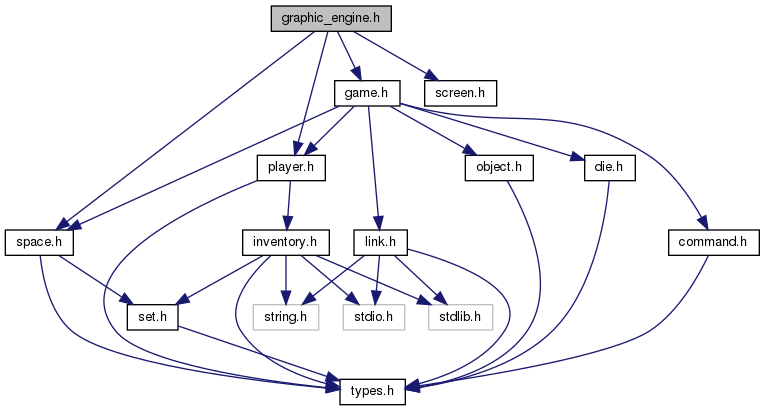
\includegraphics[width=350pt]{graphic__engine_8h__incl}
\end{center}
\end{figure}
This graph shows which files directly or indirectly include this file\+:\nopagebreak
\begin{figure}[H]
\begin{center}
\leavevmode
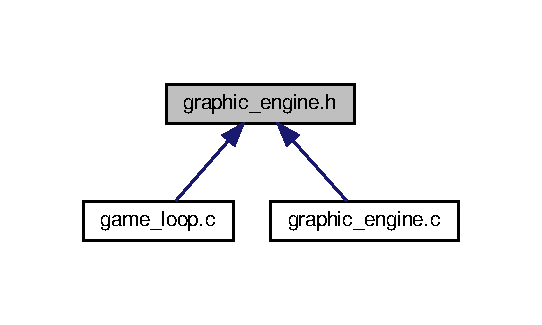
\includegraphics[width=260pt]{graphic__engine_8h__dep__incl}
\end{center}
\end{figure}
\subsection*{Macros}
\begin{DoxyCompactItemize}
\item 
\#define \hyperlink{graphic__engine_8h_aad732d3eb468a71e3179db5799c19238}{T\+A\+M\+\_\+\+C\+A\+S\+I\+L\+LA}~13
\item 
\#define \hyperlink{graphic__engine_8h_aa2d6ccbb8c91b54681c0f1dcc1b59441}{T\+A\+M\+\_\+\+T\+O\+T\+A\+L\+\_\+\+C\+A\+S\+I\+L\+LA}~20
\end{DoxyCompactItemize}
\subsection*{Typedefs}
\begin{DoxyCompactItemize}
\item 
typedef struct \hyperlink{struct__Graphic__engine}{\+\_\+\+Graphic\+\_\+engine} \hyperlink{graphic__engine_8h_ae1bc5cdbfce93098f066274fdea49af1}{Graphic\+\_\+engine}
\end{DoxyCompactItemize}
\subsection*{Functions}
\begin{DoxyCompactItemize}
\item 
\hyperlink{graphic__engine_8h_ae1bc5cdbfce93098f066274fdea49af1}{Graphic\+\_\+engine} $\ast$ \hyperlink{graphic__engine_8h_a8c3d9abe7282bee1d77d23ea80a4bdec}{graphic\+\_\+engine\+\_\+create} ()
\begin{DoxyCompactList}\small\item\em crea una interfaz grafica \end{DoxyCompactList}\item 
void \hyperlink{graphic__engine_8h_a5a5eac4ef2033c5ad71aa6895f362f79}{graphic\+\_\+engine\+\_\+destroy} (\hyperlink{graphic__engine_8h_ae1bc5cdbfce93098f066274fdea49af1}{Graphic\+\_\+engine} $\ast$ge)
\begin{DoxyCompactList}\small\item\em destruye una interfaz grafica \end{DoxyCompactList}\item 
void \hyperlink{graphic__engine_8h_a0e275aa477d5fa59e903da33a2a40a5d}{graphic\+\_\+engine\+\_\+paint\+\_\+game} (\hyperlink{graphic__engine_8h_ae1bc5cdbfce93098f066274fdea49af1}{Graphic\+\_\+engine} $\ast$ge, \hyperlink{game_8h_a57156d39c530aec3fba3a9dad8c2dc6a}{Game} $\ast$game)
\begin{DoxyCompactList}\small\item\em hace la interfaz grafica del juego \end{DoxyCompactList}\end{DoxyCompactItemize}


\subsection{Detailed Description}
En este fichero estaran las funciones relacionadas con la interfaz gráfica. 

\begin{DoxyAuthor}{Author}
Manuel Suarez, Saul Almazán, Álvaro Becerra, Rodrigo Lardiés 
\end{DoxyAuthor}
\begin{DoxyVersion}{Version}
2.\+0 
\end{DoxyVersion}
\begin{DoxyDate}{Date}
8/11/2018 
\end{DoxyDate}


\subsection{Macro Definition Documentation}
\mbox{\Hypertarget{graphic__engine_8h_aad732d3eb468a71e3179db5799c19238}\label{graphic__engine_8h_aad732d3eb468a71e3179db5799c19238}} 
\index{graphic\+\_\+engine.\+h@{graphic\+\_\+engine.\+h}!T\+A\+M\+\_\+\+C\+A\+S\+I\+L\+LA@{T\+A\+M\+\_\+\+C\+A\+S\+I\+L\+LA}}
\index{T\+A\+M\+\_\+\+C\+A\+S\+I\+L\+LA@{T\+A\+M\+\_\+\+C\+A\+S\+I\+L\+LA}!graphic\+\_\+engine.\+h@{graphic\+\_\+engine.\+h}}
\subsubsection{\texorpdfstring{T\+A\+M\+\_\+\+C\+A\+S\+I\+L\+LA}{TAM\_CASILLA}}
{\footnotesize\ttfamily \#define T\+A\+M\+\_\+\+C\+A\+S\+I\+L\+LA~13}

Número de espacios en blanco en una casilla entre las dos $\vert$ \mbox{\Hypertarget{graphic__engine_8h_aa2d6ccbb8c91b54681c0f1dcc1b59441}\label{graphic__engine_8h_aa2d6ccbb8c91b54681c0f1dcc1b59441}} 
\index{graphic\+\_\+engine.\+h@{graphic\+\_\+engine.\+h}!T\+A\+M\+\_\+\+T\+O\+T\+A\+L\+\_\+\+C\+A\+S\+I\+L\+LA@{T\+A\+M\+\_\+\+T\+O\+T\+A\+L\+\_\+\+C\+A\+S\+I\+L\+LA}}
\index{T\+A\+M\+\_\+\+T\+O\+T\+A\+L\+\_\+\+C\+A\+S\+I\+L\+LA@{T\+A\+M\+\_\+\+T\+O\+T\+A\+L\+\_\+\+C\+A\+S\+I\+L\+LA}!graphic\+\_\+engine.\+h@{graphic\+\_\+engine.\+h}}
\subsubsection{\texorpdfstring{T\+A\+M\+\_\+\+T\+O\+T\+A\+L\+\_\+\+C\+A\+S\+I\+L\+LA}{TAM\_TOTAL\_CASILLA}}
{\footnotesize\ttfamily \#define T\+A\+M\+\_\+\+T\+O\+T\+A\+L\+\_\+\+C\+A\+S\+I\+L\+LA~20}

Caracteres máximos de una casilla 

\subsection{Typedef Documentation}
\mbox{\Hypertarget{graphic__engine_8h_ae1bc5cdbfce93098f066274fdea49af1}\label{graphic__engine_8h_ae1bc5cdbfce93098f066274fdea49af1}} 
\index{graphic\+\_\+engine.\+h@{graphic\+\_\+engine.\+h}!Graphic\+\_\+engine@{Graphic\+\_\+engine}}
\index{Graphic\+\_\+engine@{Graphic\+\_\+engine}!graphic\+\_\+engine.\+h@{graphic\+\_\+engine.\+h}}
\subsubsection{\texorpdfstring{Graphic\+\_\+engine}{Graphic\_engine}}
{\footnotesize\ttfamily typedef struct \hyperlink{struct__Graphic__engine}{\+\_\+\+Graphic\+\_\+engine} \hyperlink{graphic__engine_8h_ae1bc5cdbfce93098f066274fdea49af1}{Graphic\+\_\+engine}}

Estructura de la interfaz grafica 

\subsection{Function Documentation}
\mbox{\Hypertarget{graphic__engine_8h_a8c3d9abe7282bee1d77d23ea80a4bdec}\label{graphic__engine_8h_a8c3d9abe7282bee1d77d23ea80a4bdec}} 
\index{graphic\+\_\+engine.\+h@{graphic\+\_\+engine.\+h}!graphic\+\_\+engine\+\_\+create@{graphic\+\_\+engine\+\_\+create}}
\index{graphic\+\_\+engine\+\_\+create@{graphic\+\_\+engine\+\_\+create}!graphic\+\_\+engine.\+h@{graphic\+\_\+engine.\+h}}
\subsubsection{\texorpdfstring{graphic\+\_\+engine\+\_\+create()}{graphic\_engine\_create()}}
{\footnotesize\ttfamily \hyperlink{graphic__engine_8h_ae1bc5cdbfce93098f066274fdea49af1}{Graphic\+\_\+engine}$\ast$ graphic\+\_\+engine\+\_\+create (\begin{DoxyParamCaption}{ }\end{DoxyParamCaption})}



crea una interfaz grafica 

\begin{DoxyAuthor}{Author}
Manuel Suarez, Saul Almazán, Álvaro Becerra, Rodrigo Lardiés 
\end{DoxyAuthor}
\begin{DoxyDate}{Date}
8/11/2018 
\end{DoxyDate}
\begin{DoxyReturn}{Returns}
Graphic\+\_\+engine (la interfaz que hemos creado) 
\end{DoxyReturn}
\mbox{\Hypertarget{graphic__engine_8h_a5a5eac4ef2033c5ad71aa6895f362f79}\label{graphic__engine_8h_a5a5eac4ef2033c5ad71aa6895f362f79}} 
\index{graphic\+\_\+engine.\+h@{graphic\+\_\+engine.\+h}!graphic\+\_\+engine\+\_\+destroy@{graphic\+\_\+engine\+\_\+destroy}}
\index{graphic\+\_\+engine\+\_\+destroy@{graphic\+\_\+engine\+\_\+destroy}!graphic\+\_\+engine.\+h@{graphic\+\_\+engine.\+h}}
\subsubsection{\texorpdfstring{graphic\+\_\+engine\+\_\+destroy()}{graphic\_engine\_destroy()}}
{\footnotesize\ttfamily void graphic\+\_\+engine\+\_\+destroy (\begin{DoxyParamCaption}\item[{\hyperlink{graphic__engine_8h_ae1bc5cdbfce93098f066274fdea49af1}{Graphic\+\_\+engine} $\ast$}]{ge }\end{DoxyParamCaption})}



destruye una interfaz grafica 

\begin{DoxyAuthor}{Author}
Manuel Suarez, Saul Almazán, Álvaro Becerra, Rodrigo Lardiés 
\end{DoxyAuthor}
\begin{DoxyDate}{Date}
8/11/2018 
\end{DoxyDate}

\begin{DoxyParams}{Parameters}
{\em ge} & (la interfaz que se va a destruir) \\
\hline
\end{DoxyParams}
\begin{DoxyReturn}{Returns}
void (no devuelve nada) 
\end{DoxyReturn}
\mbox{\Hypertarget{graphic__engine_8h_a0e275aa477d5fa59e903da33a2a40a5d}\label{graphic__engine_8h_a0e275aa477d5fa59e903da33a2a40a5d}} 
\index{graphic\+\_\+engine.\+h@{graphic\+\_\+engine.\+h}!graphic\+\_\+engine\+\_\+paint\+\_\+game@{graphic\+\_\+engine\+\_\+paint\+\_\+game}}
\index{graphic\+\_\+engine\+\_\+paint\+\_\+game@{graphic\+\_\+engine\+\_\+paint\+\_\+game}!graphic\+\_\+engine.\+h@{graphic\+\_\+engine.\+h}}
\subsubsection{\texorpdfstring{graphic\+\_\+engine\+\_\+paint\+\_\+game()}{graphic\_engine\_paint\_game()}}
{\footnotesize\ttfamily void graphic\+\_\+engine\+\_\+paint\+\_\+game (\begin{DoxyParamCaption}\item[{\hyperlink{graphic__engine_8h_ae1bc5cdbfce93098f066274fdea49af1}{Graphic\+\_\+engine} $\ast$}]{ge,  }\item[{\hyperlink{game_8h_a57156d39c530aec3fba3a9dad8c2dc6a}{Game} $\ast$}]{game }\end{DoxyParamCaption})}



hace la interfaz grafica del juego 

\begin{DoxyAuthor}{Author}
Manuel Suarez, Saul Almazán, Álvaro Becerra, Rodrigo Lardiés 
\end{DoxyAuthor}
\begin{DoxyDate}{Date}
8/11/2018 
\end{DoxyDate}

\begin{DoxyParams}{Parameters}
{\em ge} & (la interfaz que se va a usar) \\
\hline
{\em game} & (El juego que se va a usar) \\
\hline
\end{DoxyParams}
\begin{DoxyReturn}{Returns}
void (no devuelve nada) 
\end{DoxyReturn}

\hypertarget{inventory_8h}{}\section{inventory.\+h File Reference}
\label{inventory_8h}\index{inventory.\+h@{inventory.\+h}}


En este fichero implementamos las funciones del inventario.  


{\ttfamily \#include $<$stdio.\+h$>$}\newline
{\ttfamily \#include $<$stdlib.\+h$>$}\newline
{\ttfamily \#include $<$string.\+h$>$}\newline
{\ttfamily \#include \char`\"{}types.\+h\char`\"{}}\newline
{\ttfamily \#include \char`\"{}set.\+h\char`\"{}}\newline
Include dependency graph for inventory.\+h\+:\nopagebreak
\begin{figure}[H]
\begin{center}
\leavevmode
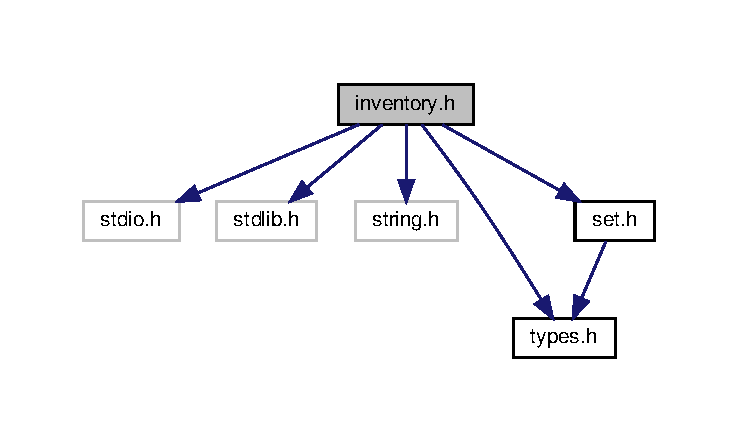
\includegraphics[width=350pt]{inventory_8h__incl}
\end{center}
\end{figure}
This graph shows which files directly or indirectly include this file\+:\nopagebreak
\begin{figure}[H]
\begin{center}
\leavevmode
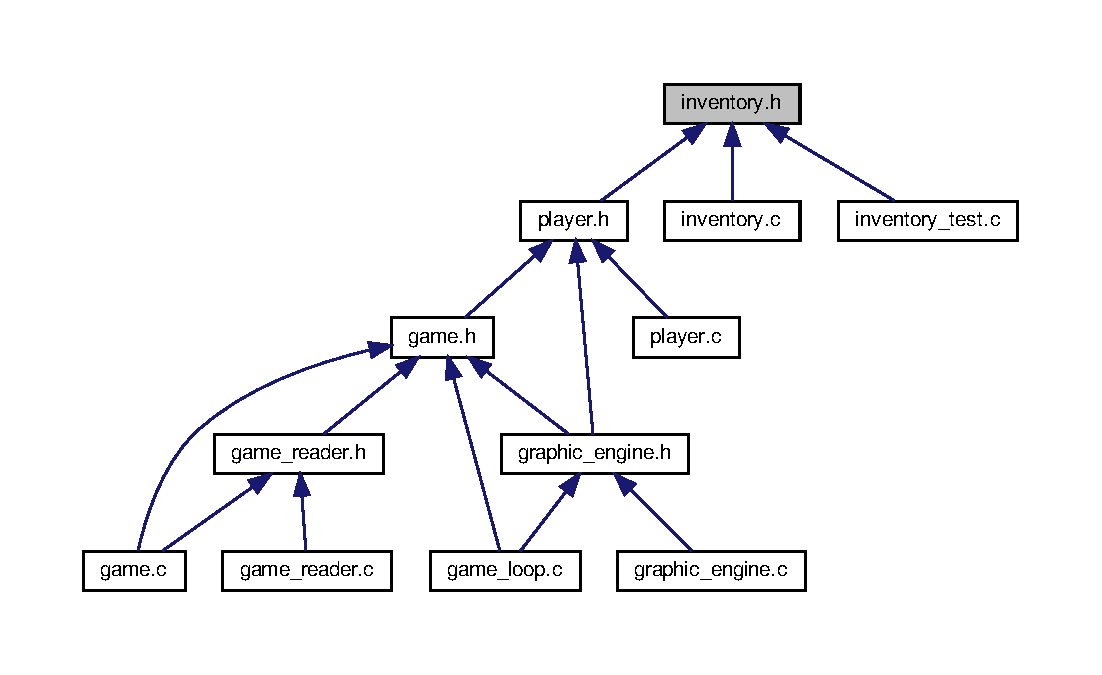
\includegraphics[width=350pt]{inventory_8h__dep__incl}
\end{center}
\end{figure}
\subsection*{Typedefs}
\begin{DoxyCompactItemize}
\item 
typedef struct \hyperlink{struct__Inventory}{\+\_\+\+Inventory} \hyperlink{inventory_8h_a2253bf64ac4ce6a9c1d6f39c0b0d32a3}{Inventory}
\end{DoxyCompactItemize}
\subsection*{Functions}
\begin{DoxyCompactItemize}
\item 
\hyperlink{inventory_8h_a2253bf64ac4ce6a9c1d6f39c0b0d32a3}{Inventory} $\ast$ \hyperlink{inventory_8h_af7029a1a54b97f41fbd9f8437bf55ff9}{inventory\+\_\+create} (int tam)
\begin{DoxyCompactList}\small\item\em crea un inventario \end{DoxyCompactList}\item 
\hyperlink{types_8h_a32c27cc471df37f4fc818d65de0a56c4}{S\+T\+A\+T\+US} \hyperlink{inventory_8h_a654cebc804053355650fc71c49e79169}{inventory\+\_\+destroy} (\hyperlink{inventory_8h_a2253bf64ac4ce6a9c1d6f39c0b0d32a3}{Inventory} $\ast$bag)
\begin{DoxyCompactList}\small\item\em destruye un inventario \end{DoxyCompactList}\item 
\hyperlink{types_8h_a3e5b8192e7d9ffaf3542f1210aec18dd}{B\+O\+OL} \hyperlink{inventory_8h_a8284d16f802fe1225be5a34f0616dffd}{inventory\+\_\+is\+\_\+full} (\hyperlink{inventory_8h_a2253bf64ac4ce6a9c1d6f39c0b0d32a3}{Inventory} $\ast$bag)
\begin{DoxyCompactList}\small\item\em comprueba si el inventario esta lleno \end{DoxyCompactList}\item 
\hyperlink{types_8h_a3e5b8192e7d9ffaf3542f1210aec18dd}{B\+O\+OL} \hyperlink{inventory_8h_a2e42d41ecfb69141831596f72cd7d694}{inventory\+\_\+is\+\_\+empty} (\hyperlink{inventory_8h_a2253bf64ac4ce6a9c1d6f39c0b0d32a3}{Inventory} $\ast$bag)
\begin{DoxyCompactList}\small\item\em comprueba si el inventario esta vacio \end{DoxyCompactList}\item 
\hyperlink{types_8h_a3e5b8192e7d9ffaf3542f1210aec18dd}{B\+O\+OL} \hyperlink{inventory_8h_a15b54a6371860e214875899f790504b1}{inventory\+\_\+is\+\_\+object\+\_\+in} (\hyperlink{inventory_8h_a2253bf64ac4ce6a9c1d6f39c0b0d32a3}{Inventory} $\ast$bag, \hyperlink{types_8h_a845e604fb28f7e3d97549da3448149d3}{Id} id)
\begin{DoxyCompactList}\small\item\em comprueba si el objeto esta en el inventario \end{DoxyCompactList}\item 
\hyperlink{types_8h_a32c27cc471df37f4fc818d65de0a56c4}{S\+T\+A\+T\+US} \hyperlink{inventory_8h_a7bdb60da746304e8e80af87fb9c7ca92}{inventory\+\_\+add\+\_\+object} (\hyperlink{inventory_8h_a2253bf64ac4ce6a9c1d6f39c0b0d32a3}{Inventory} $\ast$bag, \hyperlink{types_8h_a845e604fb28f7e3d97549da3448149d3}{Id} id)
\begin{DoxyCompactList}\small\item\em añade un objeto del inventario \end{DoxyCompactList}\item 
\hyperlink{types_8h_a32c27cc471df37f4fc818d65de0a56c4}{S\+T\+A\+T\+US} \hyperlink{inventory_8h_a8b507ba4c2009e194c6338dd609186aa}{inventory\+\_\+delete\+\_\+object} (\hyperlink{inventory_8h_a2253bf64ac4ce6a9c1d6f39c0b0d32a3}{Inventory} $\ast$bag, \hyperlink{types_8h_a845e604fb28f7e3d97549da3448149d3}{Id} id)
\begin{DoxyCompactList}\small\item\em quita un objeto del inventario \end{DoxyCompactList}\item 
\hyperlink{set_8h_a6d3b7f7c92cbb4577ef3ef7ddbf93161}{Set} $\ast$ \hyperlink{inventory_8h_a60c25937b75342b2db4c18f3c21ace5f}{inventory\+\_\+get\+\_\+set} (\hyperlink{inventory_8h_a2253bf64ac4ce6a9c1d6f39c0b0d32a3}{Inventory} $\ast$bag)
\begin{DoxyCompactList}\small\item\em devuelve los objetos del inventario \end{DoxyCompactList}\item 
int \hyperlink{inventory_8h_ae13ea773456a53a0de513478940087a4}{inventory\+\_\+get\+\_\+size} (\hyperlink{inventory_8h_a2253bf64ac4ce6a9c1d6f39c0b0d32a3}{Inventory} $\ast$bag)
\begin{DoxyCompactList}\small\item\em devuelve el tamaño de un inventario \end{DoxyCompactList}\item 
\hyperlink{types_8h_a32c27cc471df37f4fc818d65de0a56c4}{S\+T\+A\+T\+US} \hyperlink{inventory_8h_aaf549db330cb81b574a0437ee8674e95}{inventory\+\_\+set\+\_\+set} (\hyperlink{inventory_8h_a2253bf64ac4ce6a9c1d6f39c0b0d32a3}{Inventory} $\ast$bag, \hyperlink{set_8h_a6d3b7f7c92cbb4577ef3ef7ddbf93161}{Set} $\ast$set)
\begin{DoxyCompactList}\small\item\em modifica los objetos de un inventario \end{DoxyCompactList}\item 
\hyperlink{types_8h_a32c27cc471df37f4fc818d65de0a56c4}{S\+T\+A\+T\+US} \hyperlink{inventory_8h_a4823fd1e3eb0d1d97d36600dafa0a78c}{inventory\+\_\+set\+\_\+size} (\hyperlink{inventory_8h_a2253bf64ac4ce6a9c1d6f39c0b0d32a3}{Inventory} $\ast$bag, int tam)
\begin{DoxyCompactList}\small\item\em cambia el tamaño de un inventario \end{DoxyCompactList}\item 
void \hyperlink{inventory_8h_a04e305db993339cf15c45aad1fa50144}{inventory\+\_\+print} (\hyperlink{inventory_8h_a2253bf64ac4ce6a9c1d6f39c0b0d32a3}{Inventory} $\ast$bag, F\+I\+LE $\ast$filename)
\begin{DoxyCompactList}\small\item\em imprime un inventario \end{DoxyCompactList}\end{DoxyCompactItemize}


\subsection{Detailed Description}
En este fichero implementamos las funciones del inventario. 

\begin{DoxyAuthor}{Author}
Manuel Suarez, Saul Almazán, Álvaro Becerra, Rodrigo Lardiés 
\end{DoxyAuthor}
\begin{DoxyVersion}{Version}
1.\+0 
\end{DoxyVersion}
\begin{DoxyDate}{Date}
10/11/2018 
\end{DoxyDate}


\subsection{Typedef Documentation}
\mbox{\Hypertarget{inventory_8h_a2253bf64ac4ce6a9c1d6f39c0b0d32a3}\label{inventory_8h_a2253bf64ac4ce6a9c1d6f39c0b0d32a3}} 
\index{inventory.\+h@{inventory.\+h}!Inventory@{Inventory}}
\index{Inventory@{Inventory}!inventory.\+h@{inventory.\+h}}
\subsubsection{\texorpdfstring{Inventory}{Inventory}}
{\footnotesize\ttfamily typedef struct \hyperlink{struct__Inventory}{\+\_\+\+Inventory} \hyperlink{inventory_8h_a2253bf64ac4ce6a9c1d6f39c0b0d32a3}{Inventory}}

Estructura del inventario 

\subsection{Function Documentation}
\mbox{\Hypertarget{inventory_8h_a7bdb60da746304e8e80af87fb9c7ca92}\label{inventory_8h_a7bdb60da746304e8e80af87fb9c7ca92}} 
\index{inventory.\+h@{inventory.\+h}!inventory\+\_\+add\+\_\+object@{inventory\+\_\+add\+\_\+object}}
\index{inventory\+\_\+add\+\_\+object@{inventory\+\_\+add\+\_\+object}!inventory.\+h@{inventory.\+h}}
\subsubsection{\texorpdfstring{inventory\+\_\+add\+\_\+object()}{inventory\_add\_object()}}
{\footnotesize\ttfamily \hyperlink{types_8h_a32c27cc471df37f4fc818d65de0a56c4}{S\+T\+A\+T\+US} inventory\+\_\+add\+\_\+object (\begin{DoxyParamCaption}\item[{\hyperlink{inventory_8h_a2253bf64ac4ce6a9c1d6f39c0b0d32a3}{Inventory} $\ast$}]{bag,  }\item[{\hyperlink{types_8h_a845e604fb28f7e3d97549da3448149d3}{Id}}]{id }\end{DoxyParamCaption})}



añade un objeto del inventario 

\begin{DoxyAuthor}{Author}
Manuel Suarez, Saul Almazán, Álvaro Becerra, Rodrigo Lardiés 
\end{DoxyAuthor}
\begin{DoxyDate}{Date}
10/11/2018 
\end{DoxyDate}

\begin{DoxyParams}{Parameters}
{\em bag} & (inventario a modificar) \\
\hline
{\em id} & (Id del objeto) \\
\hline
\end{DoxyParams}
\begin{DoxyReturn}{Returns}
S\+T\+A\+T\+US (OK si se ha realizado correctamente o E\+R\+R\+OR de lo contrario) 
\end{DoxyReturn}
\mbox{\Hypertarget{inventory_8h_af7029a1a54b97f41fbd9f8437bf55ff9}\label{inventory_8h_af7029a1a54b97f41fbd9f8437bf55ff9}} 
\index{inventory.\+h@{inventory.\+h}!inventory\+\_\+create@{inventory\+\_\+create}}
\index{inventory\+\_\+create@{inventory\+\_\+create}!inventory.\+h@{inventory.\+h}}
\subsubsection{\texorpdfstring{inventory\+\_\+create()}{inventory\_create()}}
{\footnotesize\ttfamily \hyperlink{inventory_8h_a2253bf64ac4ce6a9c1d6f39c0b0d32a3}{Inventory}$\ast$ inventory\+\_\+create (\begin{DoxyParamCaption}\item[{int}]{tam }\end{DoxyParamCaption})}



crea un inventario 

\begin{DoxyAuthor}{Author}
Manuel Suarez, Saul Almazán, Álvaro Becerra, Rodrigo Lardiés 
\end{DoxyAuthor}
\begin{DoxyDate}{Date}
10/11/2018 
\end{DoxyDate}

\begin{DoxyParams}{Parameters}
{\em tam} & (tamaño del inventario) \\
\hline
\end{DoxyParams}
\begin{DoxyReturn}{Returns}
inventory (El inventario que crea)
\end{DoxyReturn}
\begin{DoxyAuthor}{Author}
Manuel Suarez, Saul Almazán, Álvaro Becerra, Rodrigo Lardiés 
\end{DoxyAuthor}
\begin{DoxyDate}{Date}
10/11/2018 
\end{DoxyDate}

\begin{DoxyParams}{Parameters}
{\em tam} & (tamaño del inventario) \\
\hline
\end{DoxyParams}
\begin{DoxyReturn}{Returns}
inventory$\ast$ (El inventario que crea) 
\end{DoxyReturn}
\mbox{\Hypertarget{inventory_8h_a8b507ba4c2009e194c6338dd609186aa}\label{inventory_8h_a8b507ba4c2009e194c6338dd609186aa}} 
\index{inventory.\+h@{inventory.\+h}!inventory\+\_\+delete\+\_\+object@{inventory\+\_\+delete\+\_\+object}}
\index{inventory\+\_\+delete\+\_\+object@{inventory\+\_\+delete\+\_\+object}!inventory.\+h@{inventory.\+h}}
\subsubsection{\texorpdfstring{inventory\+\_\+delete\+\_\+object()}{inventory\_delete\_object()}}
{\footnotesize\ttfamily \hyperlink{types_8h_a32c27cc471df37f4fc818d65de0a56c4}{S\+T\+A\+T\+US} inventory\+\_\+delete\+\_\+object (\begin{DoxyParamCaption}\item[{\hyperlink{inventory_8h_a2253bf64ac4ce6a9c1d6f39c0b0d32a3}{Inventory} $\ast$}]{bag,  }\item[{\hyperlink{types_8h_a845e604fb28f7e3d97549da3448149d3}{Id}}]{id }\end{DoxyParamCaption})}



quita un objeto del inventario 

\begin{DoxyAuthor}{Author}
Manuel Suarez, Saul Almazán, Álvaro Becerra, Rodrigo Lardiés 
\end{DoxyAuthor}
\begin{DoxyDate}{Date}
10/11/2018 
\end{DoxyDate}

\begin{DoxyParams}{Parameters}
{\em bag} & (inventario a modificar) \\
\hline
{\em id} & (Id del objeto) \\
\hline
\end{DoxyParams}
\begin{DoxyReturn}{Returns}
S\+T\+A\+T\+US (OK si se ha realizado correctamente o E\+R\+R\+OR de lo contrario) 
\end{DoxyReturn}
\mbox{\Hypertarget{inventory_8h_a654cebc804053355650fc71c49e79169}\label{inventory_8h_a654cebc804053355650fc71c49e79169}} 
\index{inventory.\+h@{inventory.\+h}!inventory\+\_\+destroy@{inventory\+\_\+destroy}}
\index{inventory\+\_\+destroy@{inventory\+\_\+destroy}!inventory.\+h@{inventory.\+h}}
\subsubsection{\texorpdfstring{inventory\+\_\+destroy()}{inventory\_destroy()}}
{\footnotesize\ttfamily \hyperlink{types_8h_a32c27cc471df37f4fc818d65de0a56c4}{S\+T\+A\+T\+US} inventory\+\_\+destroy (\begin{DoxyParamCaption}\item[{\hyperlink{inventory_8h_a2253bf64ac4ce6a9c1d6f39c0b0d32a3}{Inventory} $\ast$}]{bag }\end{DoxyParamCaption})}



destruye un inventario 

\begin{DoxyAuthor}{Author}
Manuel Suarez, Saul Almazán, Álvaro Becerra, Rodrigo Lardiés 
\end{DoxyAuthor}
\begin{DoxyDate}{Date}
10/11/2018 
\end{DoxyDate}

\begin{DoxyParams}{Parameters}
{\em bag} & (inventario a destruir) \\
\hline
\end{DoxyParams}
\begin{DoxyReturn}{Returns}
S\+T\+A\+T\+US (OK si se ha realizado correctamente o E\+R\+R\+OR de lo contrario) 
\end{DoxyReturn}
\mbox{\Hypertarget{inventory_8h_a60c25937b75342b2db4c18f3c21ace5f}\label{inventory_8h_a60c25937b75342b2db4c18f3c21ace5f}} 
\index{inventory.\+h@{inventory.\+h}!inventory\+\_\+get\+\_\+set@{inventory\+\_\+get\+\_\+set}}
\index{inventory\+\_\+get\+\_\+set@{inventory\+\_\+get\+\_\+set}!inventory.\+h@{inventory.\+h}}
\subsubsection{\texorpdfstring{inventory\+\_\+get\+\_\+set()}{inventory\_get\_set()}}
{\footnotesize\ttfamily \hyperlink{set_8h_a6d3b7f7c92cbb4577ef3ef7ddbf93161}{Set}$\ast$ inventory\+\_\+get\+\_\+set (\begin{DoxyParamCaption}\item[{\hyperlink{inventory_8h_a2253bf64ac4ce6a9c1d6f39c0b0d32a3}{Inventory} $\ast$}]{bag }\end{DoxyParamCaption})}



devuelve los objetos del inventario 

\begin{DoxyAuthor}{Author}
Manuel Suarez, Saul Almazán, Álvaro Becerra, Rodrigo Lardiés 
\end{DoxyAuthor}
\begin{DoxyDate}{Date}
10/11/2018 
\end{DoxyDate}

\begin{DoxyParams}{Parameters}
{\em bag} & (inventario a destruir) \\
\hline
\end{DoxyParams}
\begin{DoxyReturn}{Returns}
Set (Objetos del inventario) 
\end{DoxyReturn}
\mbox{\Hypertarget{inventory_8h_ae13ea773456a53a0de513478940087a4}\label{inventory_8h_ae13ea773456a53a0de513478940087a4}} 
\index{inventory.\+h@{inventory.\+h}!inventory\+\_\+get\+\_\+size@{inventory\+\_\+get\+\_\+size}}
\index{inventory\+\_\+get\+\_\+size@{inventory\+\_\+get\+\_\+size}!inventory.\+h@{inventory.\+h}}
\subsubsection{\texorpdfstring{inventory\+\_\+get\+\_\+size()}{inventory\_get\_size()}}
{\footnotesize\ttfamily int inventory\+\_\+get\+\_\+size (\begin{DoxyParamCaption}\item[{\hyperlink{inventory_8h_a2253bf64ac4ce6a9c1d6f39c0b0d32a3}{Inventory} $\ast$}]{bag }\end{DoxyParamCaption})}



devuelve el tamaño de un inventario 

\begin{DoxyAuthor}{Author}
Manuel Suarez, Saul Almazán, Álvaro Becerra, Rodrigo Lardiés 
\end{DoxyAuthor}
\begin{DoxyDate}{Date}
10/11/2018 
\end{DoxyDate}

\begin{DoxyParams}{Parameters}
{\em bag} & (inventario a usar) \\
\hline
\end{DoxyParams}
\begin{DoxyReturn}{Returns}
int (Tamaño del inventario) 
\end{DoxyReturn}
\mbox{\Hypertarget{inventory_8h_a2e42d41ecfb69141831596f72cd7d694}\label{inventory_8h_a2e42d41ecfb69141831596f72cd7d694}} 
\index{inventory.\+h@{inventory.\+h}!inventory\+\_\+is\+\_\+empty@{inventory\+\_\+is\+\_\+empty}}
\index{inventory\+\_\+is\+\_\+empty@{inventory\+\_\+is\+\_\+empty}!inventory.\+h@{inventory.\+h}}
\subsubsection{\texorpdfstring{inventory\+\_\+is\+\_\+empty()}{inventory\_is\_empty()}}
{\footnotesize\ttfamily \hyperlink{types_8h_a3e5b8192e7d9ffaf3542f1210aec18dd}{B\+O\+OL} inventory\+\_\+is\+\_\+empty (\begin{DoxyParamCaption}\item[{\hyperlink{inventory_8h_a2253bf64ac4ce6a9c1d6f39c0b0d32a3}{Inventory} $\ast$}]{bag }\end{DoxyParamCaption})}



comprueba si el inventario esta vacio 

\begin{DoxyAuthor}{Author}
Manuel Suarez, Saul Almazán, Álvaro Becerra, Rodrigo Lardiés 
\end{DoxyAuthor}
\begin{DoxyDate}{Date}
10/11/2018 
\end{DoxyDate}

\begin{DoxyParams}{Parameters}
{\em bag} & (inventario a usar) \\
\hline
\end{DoxyParams}
\begin{DoxyReturn}{Returns}
B\+O\+OL (T\+R\+UE si esta vacio o F\+A\+L\+SE de lo contrario) 
\end{DoxyReturn}
\mbox{\Hypertarget{inventory_8h_a8284d16f802fe1225be5a34f0616dffd}\label{inventory_8h_a8284d16f802fe1225be5a34f0616dffd}} 
\index{inventory.\+h@{inventory.\+h}!inventory\+\_\+is\+\_\+full@{inventory\+\_\+is\+\_\+full}}
\index{inventory\+\_\+is\+\_\+full@{inventory\+\_\+is\+\_\+full}!inventory.\+h@{inventory.\+h}}
\subsubsection{\texorpdfstring{inventory\+\_\+is\+\_\+full()}{inventory\_is\_full()}}
{\footnotesize\ttfamily \hyperlink{types_8h_a3e5b8192e7d9ffaf3542f1210aec18dd}{B\+O\+OL} inventory\+\_\+is\+\_\+full (\begin{DoxyParamCaption}\item[{\hyperlink{inventory_8h_a2253bf64ac4ce6a9c1d6f39c0b0d32a3}{Inventory} $\ast$}]{bag }\end{DoxyParamCaption})}



comprueba si el inventario esta lleno 

\begin{DoxyAuthor}{Author}
Manuel Suarez, Saul Almazán, Álvaro Becerra, Rodrigo Lardiés 
\end{DoxyAuthor}
\begin{DoxyDate}{Date}
10/11/2018 
\end{DoxyDate}

\begin{DoxyParams}{Parameters}
{\em bag} & (inventario a usar) \\
\hline
\end{DoxyParams}
\begin{DoxyReturn}{Returns}
B\+O\+OL (T\+R\+UE si esta lleno o F\+A\+L\+SE de lo contrario) 
\end{DoxyReturn}
\mbox{\Hypertarget{inventory_8h_a15b54a6371860e214875899f790504b1}\label{inventory_8h_a15b54a6371860e214875899f790504b1}} 
\index{inventory.\+h@{inventory.\+h}!inventory\+\_\+is\+\_\+object\+\_\+in@{inventory\+\_\+is\+\_\+object\+\_\+in}}
\index{inventory\+\_\+is\+\_\+object\+\_\+in@{inventory\+\_\+is\+\_\+object\+\_\+in}!inventory.\+h@{inventory.\+h}}
\subsubsection{\texorpdfstring{inventory\+\_\+is\+\_\+object\+\_\+in()}{inventory\_is\_object\_in()}}
{\footnotesize\ttfamily \hyperlink{types_8h_a3e5b8192e7d9ffaf3542f1210aec18dd}{B\+O\+OL} inventory\+\_\+is\+\_\+object\+\_\+in (\begin{DoxyParamCaption}\item[{\hyperlink{inventory_8h_a2253bf64ac4ce6a9c1d6f39c0b0d32a3}{Inventory} $\ast$}]{bag,  }\item[{\hyperlink{types_8h_a845e604fb28f7e3d97549da3448149d3}{Id}}]{id }\end{DoxyParamCaption})}



comprueba si el objeto esta en el inventario 

\begin{DoxyAuthor}{Author}
Manuel Suarez, Saul Almazán, Álvaro Becerra, Rodrigo Lardiés 
\end{DoxyAuthor}
\begin{DoxyDate}{Date}
10/11/2018 
\end{DoxyDate}

\begin{DoxyParams}{Parameters}
{\em bag} & (inventario a usar) \\
\hline
{\em id} & (Id del objeto) \\
\hline
\end{DoxyParams}
\begin{DoxyReturn}{Returns}
B\+O\+OL (T\+R\+UE si esta en el inventario o F\+A\+L\+SE de lo contrario) 
\end{DoxyReturn}
\mbox{\Hypertarget{inventory_8h_a04e305db993339cf15c45aad1fa50144}\label{inventory_8h_a04e305db993339cf15c45aad1fa50144}} 
\index{inventory.\+h@{inventory.\+h}!inventory\+\_\+print@{inventory\+\_\+print}}
\index{inventory\+\_\+print@{inventory\+\_\+print}!inventory.\+h@{inventory.\+h}}
\subsubsection{\texorpdfstring{inventory\+\_\+print()}{inventory\_print()}}
{\footnotesize\ttfamily void inventory\+\_\+print (\begin{DoxyParamCaption}\item[{\hyperlink{inventory_8h_a2253bf64ac4ce6a9c1d6f39c0b0d32a3}{Inventory} $\ast$}]{bag,  }\item[{F\+I\+LE $\ast$}]{filename }\end{DoxyParamCaption})}



imprime un inventario 

\begin{DoxyAuthor}{Author}
Manuel Suarez, Saul Almazán, Álvaro Becerra, Rodrigo Lardiés 
\end{DoxyAuthor}
\begin{DoxyDate}{Date}
10/11/2018 
\end{DoxyDate}

\begin{DoxyParams}{Parameters}
{\em bag} & (inventario a imprimir) \\
\hline
{\em filename} & (Donde se imprime) \\
\hline
\end{DoxyParams}
\begin{DoxyReturn}{Returns}
void (No devuelve nada) 
\end{DoxyReturn}
\mbox{\Hypertarget{inventory_8h_aaf549db330cb81b574a0437ee8674e95}\label{inventory_8h_aaf549db330cb81b574a0437ee8674e95}} 
\index{inventory.\+h@{inventory.\+h}!inventory\+\_\+set\+\_\+set@{inventory\+\_\+set\+\_\+set}}
\index{inventory\+\_\+set\+\_\+set@{inventory\+\_\+set\+\_\+set}!inventory.\+h@{inventory.\+h}}
\subsubsection{\texorpdfstring{inventory\+\_\+set\+\_\+set()}{inventory\_set\_set()}}
{\footnotesize\ttfamily \hyperlink{types_8h_a32c27cc471df37f4fc818d65de0a56c4}{S\+T\+A\+T\+US} inventory\+\_\+set\+\_\+set (\begin{DoxyParamCaption}\item[{\hyperlink{inventory_8h_a2253bf64ac4ce6a9c1d6f39c0b0d32a3}{Inventory} $\ast$}]{bag,  }\item[{\hyperlink{set_8h_a6d3b7f7c92cbb4577ef3ef7ddbf93161}{Set} $\ast$}]{set }\end{DoxyParamCaption})}



modifica los objetos de un inventario 

\begin{DoxyAuthor}{Author}
Manuel Suarez, Saul Almazán, Álvaro Becerra, Rodrigo Lardiés 
\end{DoxyAuthor}
\begin{DoxyDate}{Date}
10/11/2018 
\end{DoxyDate}

\begin{DoxyParams}{Parameters}
{\em bag} & (inventario a modificar) \\
\hline
{\em set} & (Objetos nuevos del inventario) \\
\hline
\end{DoxyParams}
\begin{DoxyReturn}{Returns}
S\+T\+A\+T\+US (OK si se ha realizado correctamente o E\+R\+R\+OR de lo contrario) 
\end{DoxyReturn}
\mbox{\Hypertarget{inventory_8h_a4823fd1e3eb0d1d97d36600dafa0a78c}\label{inventory_8h_a4823fd1e3eb0d1d97d36600dafa0a78c}} 
\index{inventory.\+h@{inventory.\+h}!inventory\+\_\+set\+\_\+size@{inventory\+\_\+set\+\_\+size}}
\index{inventory\+\_\+set\+\_\+size@{inventory\+\_\+set\+\_\+size}!inventory.\+h@{inventory.\+h}}
\subsubsection{\texorpdfstring{inventory\+\_\+set\+\_\+size()}{inventory\_set\_size()}}
{\footnotesize\ttfamily \hyperlink{types_8h_a32c27cc471df37f4fc818d65de0a56c4}{S\+T\+A\+T\+US} inventory\+\_\+set\+\_\+size (\begin{DoxyParamCaption}\item[{\hyperlink{inventory_8h_a2253bf64ac4ce6a9c1d6f39c0b0d32a3}{Inventory} $\ast$}]{bag,  }\item[{int}]{tam }\end{DoxyParamCaption})}



cambia el tamaño de un inventario 

\begin{DoxyAuthor}{Author}
Manuel Suarez, Saul Almazán, Álvaro Becerra, Rodrigo Lardiés 
\end{DoxyAuthor}
\begin{DoxyDate}{Date}
10/11/2018 
\end{DoxyDate}

\begin{DoxyParams}{Parameters}
{\em bag} & (inventario que se va a cambiar) \\
\hline
{\em tam} & (tamaño nuevo del inventario) \\
\hline
\end{DoxyParams}
\begin{DoxyReturn}{Returns}
S\+T\+A\+T\+US (OK si se ha realizado correctamente o E\+R\+R\+OR de lo contrario) 
\end{DoxyReturn}

\hypertarget{inventory__test_8h}{}\section{include/inventory\+\_\+test.h File Reference}
\label{inventory__test_8h}\index{include/inventory\+\_\+test.\+h@{include/inventory\+\_\+test.\+h}}


Prueba del modulo player.  


This graph shows which files directly or indirectly include this file\+:
% FIG 0
\subsection*{Functions}
\begin{DoxyCompactItemize}
\item 
void \hyperlink{inventory__test_8h_a33638f1a88ae16ab8d6bee00145b82b8}{test1\+\_\+inventory\+\_\+create} ()
\item 
void \hyperlink{inventory__test_8h_a73a6080c360a8870c4ffc734e989c8b3}{test2\+\_\+inventory\+\_\+create} ()
\item 
void \hyperlink{inventory__test_8h_af6ad6f6d577b5f123f36351139c6d918}{test1\+\_\+inventory\+\_\+delete\+\_\+object} ()
\item 
void \hyperlink{inventory__test_8h_a7df95a4c69353ae9bf0766e3d13672f8}{test2\+\_\+inventory\+\_\+delete\+\_\+object} ()
\item 
void \hyperlink{inventory__test_8h_a66005d07626ca1dae670ddc7fc3a9514}{test3\+\_\+inventory\+\_\+delete\+\_\+object} ()
\item 
void \hyperlink{inventory__test_8h_abddf20d7b11937754a88fb57c9d74292}{test1\+\_\+inventory\+\_\+add\+\_\+object} ()
\item 
void \hyperlink{inventory__test_8h_aa71b62b43df77830d47caa4237ee76a2}{test2\+\_\+inventory\+\_\+add\+\_\+object} ()
\item 
void \hyperlink{inventory__test_8h_a7eb3ba387e33c42ff45331c9d9aada34}{test1\+\_\+inventory\+\_\+is\+\_\+full} ()
\item 
void \hyperlink{inventory__test_8h_a1c9e567d4919d5aaccc9580815a8a81d}{test2\+\_\+inventory\+\_\+is\+\_\+full} ()
\item 
void \hyperlink{inventory__test_8h_afe8c9730e30b58535afc0481970ab2b1}{test1\+\_\+inventory\+\_\+is\+\_\+empty} ()
\item 
void \hyperlink{inventory__test_8h_a4d2a2a4d4ba59446d013debfe9bf05dc}{test2\+\_\+inventory\+\_\+is\+\_\+empty} ()
\item 
void \hyperlink{inventory__test_8h_a8eb3230ee30561f821224f20d9143bf8}{test1\+\_\+inventory\+\_\+is\+\_\+object\+\_\+in} ()
\item 
void \hyperlink{inventory__test_8h_a837cf990de86a6b23ef85b04b8b4dec1}{test2\+\_\+inventory\+\_\+is\+\_\+object\+\_\+in} ()
\item 
void \hyperlink{inventory__test_8h_a7eb11b5f1ef5608b42ed02d5a9ab53ab}{test1\+\_\+inventory\+\_\+get\+\_\+size} ()
\item 
void \hyperlink{inventory__test_8h_ab003abf4af7d055f6b9370618327cc81}{test2\+\_\+inventory\+\_\+get\+\_\+size} ()
\item 
void \hyperlink{inventory__test_8h_a0716920727f7687a74f246a04c2977eb}{test1\+\_\+inventory\+\_\+set\+\_\+size} ()
\item 
void \hyperlink{inventory__test_8h_a2d387a2e82970e625baae0ac4c610acc}{test2\+\_\+inventory\+\_\+set\+\_\+size} ()
\end{DoxyCompactItemize}


\subsection{Detailed Description}
Prueba del modulo player. 

\begin{DoxyAuthor}{Author}
Manuel Suarez, Saul Almazán, �?lvaro Becerra, Rodrigo Lardiés 
\end{DoxyAuthor}
\begin{DoxyVersion}{Version}
1.\+0 
\end{DoxyVersion}
\begin{DoxyDate}{Date}
12-\/11-\/2018 
\end{DoxyDate}


\subsection{Function Documentation}
\mbox{\Hypertarget{inventory__test_8h_abddf20d7b11937754a88fb57c9d74292}\label{inventory__test_8h_abddf20d7b11937754a88fb57c9d74292}} 
\index{inventory\+\_\+test.\+h@{inventory\+\_\+test.\+h}!test1\+\_\+inventory\+\_\+add\+\_\+object@{test1\+\_\+inventory\+\_\+add\+\_\+object}}
\index{test1\+\_\+inventory\+\_\+add\+\_\+object@{test1\+\_\+inventory\+\_\+add\+\_\+object}!inventory\+\_\+test.\+h@{inventory\+\_\+test.\+h}}
\subsubsection{\texorpdfstring{test1\+\_\+inventory\+\_\+add\+\_\+object()}{test1\_inventory\_add\_object()}}
{\footnotesize\ttfamily void test1\+\_\+inventory\+\_\+add\+\_\+object (\begin{DoxyParamCaption}{ }\end{DoxyParamCaption})}

\begin{DoxyRefDesc}{Test}
\item[\hyperlink{test__test000172}{Test}]Prueba la función para añadir un objeto a un inventario \end{DoxyRefDesc}
\begin{DoxyPrecond}{Precondition}
id que establecer en el inventario 
\end{DoxyPrecond}
\begin{DoxyPostcond}{Postcondition}
La salida debe ser OK
\end{DoxyPostcond}
\begin{DoxyRefDesc}{Test}
\item[\hyperlink{test__test000015}{Test}]Prueba la función para añadir un objeto a un inventario \end{DoxyRefDesc}
\begin{DoxyPrecond}{Precondition}
id que establecer en el inventario 
\end{DoxyPrecond}
\begin{DoxyPostcond}{Postcondition}
La salida debe ser OK 
\end{DoxyPostcond}
\mbox{\Hypertarget{inventory__test_8h_a33638f1a88ae16ab8d6bee00145b82b8}\label{inventory__test_8h_a33638f1a88ae16ab8d6bee00145b82b8}} 
\index{inventory\+\_\+test.\+h@{inventory\+\_\+test.\+h}!test1\+\_\+inventory\+\_\+create@{test1\+\_\+inventory\+\_\+create}}
\index{test1\+\_\+inventory\+\_\+create@{test1\+\_\+inventory\+\_\+create}!inventory\+\_\+test.\+h@{inventory\+\_\+test.\+h}}
\subsubsection{\texorpdfstring{test1\+\_\+inventory\+\_\+create()}{test1\_inventory\_create()}}
{\footnotesize\ttfamily void test1\+\_\+inventory\+\_\+create (\begin{DoxyParamCaption}{ }\end{DoxyParamCaption})}

\begin{DoxyRefDesc}{Test}
\item[\hyperlink{test__test000167}{Test}]Prueba la función de creación de un inventario \end{DoxyRefDesc}
\begin{DoxyPrecond}{Precondition}
Un numero de objetos como parámetro 
\end{DoxyPrecond}
\begin{DoxyPostcond}{Postcondition}
Un puntero no nulo al inventario creado
\end{DoxyPostcond}
\begin{DoxyRefDesc}{Test}
\item[\hyperlink{test__test000010}{Test}]Prueba la función de creación de un inventario \end{DoxyRefDesc}
\begin{DoxyPrecond}{Precondition}
Un numero de objetos como parámetro 
\end{DoxyPrecond}
\begin{DoxyPostcond}{Postcondition}
Un puntero no nulo al inventario creado 
\end{DoxyPostcond}
\mbox{\Hypertarget{inventory__test_8h_af6ad6f6d577b5f123f36351139c6d918}\label{inventory__test_8h_af6ad6f6d577b5f123f36351139c6d918}} 
\index{inventory\+\_\+test.\+h@{inventory\+\_\+test.\+h}!test1\+\_\+inventory\+\_\+delete\+\_\+object@{test1\+\_\+inventory\+\_\+delete\+\_\+object}}
\index{test1\+\_\+inventory\+\_\+delete\+\_\+object@{test1\+\_\+inventory\+\_\+delete\+\_\+object}!inventory\+\_\+test.\+h@{inventory\+\_\+test.\+h}}
\subsubsection{\texorpdfstring{test1\+\_\+inventory\+\_\+delete\+\_\+object()}{test1\_inventory\_delete\_object()}}
{\footnotesize\ttfamily void test1\+\_\+inventory\+\_\+delete\+\_\+object (\begin{DoxyParamCaption}{ }\end{DoxyParamCaption})}

\begin{DoxyRefDesc}{Test}
\item[\hyperlink{test__test000169}{Test}]Prueba la función para borrar un objeto de un inventario \end{DoxyRefDesc}
\begin{DoxyPrecond}{Precondition}
Inventario con un objeto 
\end{DoxyPrecond}
\begin{DoxyPostcond}{Postcondition}
La salida debe ser OK
\end{DoxyPostcond}
\begin{DoxyRefDesc}{Test}
\item[\hyperlink{test__test000012}{Test}]Prueba la función para borrar un objeto de un inventario \end{DoxyRefDesc}
\begin{DoxyPrecond}{Precondition}
Inventario con un objeto 
\end{DoxyPrecond}
\begin{DoxyPostcond}{Postcondition}
La salida debe ser OK 
\end{DoxyPostcond}
\mbox{\Hypertarget{inventory__test_8h_a7eb11b5f1ef5608b42ed02d5a9ab53ab}\label{inventory__test_8h_a7eb11b5f1ef5608b42ed02d5a9ab53ab}} 
\index{inventory\+\_\+test.\+h@{inventory\+\_\+test.\+h}!test1\+\_\+inventory\+\_\+get\+\_\+size@{test1\+\_\+inventory\+\_\+get\+\_\+size}}
\index{test1\+\_\+inventory\+\_\+get\+\_\+size@{test1\+\_\+inventory\+\_\+get\+\_\+size}!inventory\+\_\+test.\+h@{inventory\+\_\+test.\+h}}
\subsubsection{\texorpdfstring{test1\+\_\+inventory\+\_\+get\+\_\+size()}{test1\_inventory\_get\_size()}}
{\footnotesize\ttfamily void test1\+\_\+inventory\+\_\+get\+\_\+size (\begin{DoxyParamCaption}{ }\end{DoxyParamCaption})}

\begin{DoxyRefDesc}{Test}
\item[\hyperlink{test__test000180}{Test}]Prueba la función para obtener el tamaño de un inventario \end{DoxyRefDesc}
\begin{DoxyPrecond}{Precondition}
El inventario tiene un tamaño 
\end{DoxyPrecond}
\begin{DoxyPostcond}{Postcondition}
La salida debe ser tam=3
\end{DoxyPostcond}
\begin{DoxyRefDesc}{Test}
\item[\hyperlink{test__test000023}{Test}]Prueba la función para obtener el tamaño de un inventario \end{DoxyRefDesc}
\begin{DoxyPrecond}{Precondition}
El inventario tiene un tamaño 
\end{DoxyPrecond}
\begin{DoxyPostcond}{Postcondition}
La salida debe ser tam=3 
\end{DoxyPostcond}
\mbox{\Hypertarget{inventory__test_8h_afe8c9730e30b58535afc0481970ab2b1}\label{inventory__test_8h_afe8c9730e30b58535afc0481970ab2b1}} 
\index{inventory\+\_\+test.\+h@{inventory\+\_\+test.\+h}!test1\+\_\+inventory\+\_\+is\+\_\+empty@{test1\+\_\+inventory\+\_\+is\+\_\+empty}}
\index{test1\+\_\+inventory\+\_\+is\+\_\+empty@{test1\+\_\+inventory\+\_\+is\+\_\+empty}!inventory\+\_\+test.\+h@{inventory\+\_\+test.\+h}}
\subsubsection{\texorpdfstring{test1\+\_\+inventory\+\_\+is\+\_\+empty()}{test1\_inventory\_is\_empty()}}
{\footnotesize\ttfamily void test1\+\_\+inventory\+\_\+is\+\_\+empty (\begin{DoxyParamCaption}{ }\end{DoxyParamCaption})}

\begin{DoxyRefDesc}{Test}
\item[\hyperlink{test__test000176}{Test}]Prueba la función para comprobar si un invetario está vacío \end{DoxyRefDesc}
\begin{DoxyPrecond}{Precondition}
inventario vacío 
\end{DoxyPrecond}
\begin{DoxyPostcond}{Postcondition}
La salida debe ser T\+R\+UE
\end{DoxyPostcond}
\begin{DoxyRefDesc}{Test}
\item[\hyperlink{test__test000019}{Test}]Prueba la función para comprobar si un invetario está vacío \end{DoxyRefDesc}
\begin{DoxyPrecond}{Precondition}
inventario vacío 
\end{DoxyPrecond}
\begin{DoxyPostcond}{Postcondition}
La salida debe ser T\+R\+UE 
\end{DoxyPostcond}
\mbox{\Hypertarget{inventory__test_8h_a7eb3ba387e33c42ff45331c9d9aada34}\label{inventory__test_8h_a7eb3ba387e33c42ff45331c9d9aada34}} 
\index{inventory\+\_\+test.\+h@{inventory\+\_\+test.\+h}!test1\+\_\+inventory\+\_\+is\+\_\+full@{test1\+\_\+inventory\+\_\+is\+\_\+full}}
\index{test1\+\_\+inventory\+\_\+is\+\_\+full@{test1\+\_\+inventory\+\_\+is\+\_\+full}!inventory\+\_\+test.\+h@{inventory\+\_\+test.\+h}}
\subsubsection{\texorpdfstring{test1\+\_\+inventory\+\_\+is\+\_\+full()}{test1\_inventory\_is\_full()}}
{\footnotesize\ttfamily void test1\+\_\+inventory\+\_\+is\+\_\+full (\begin{DoxyParamCaption}{ }\end{DoxyParamCaption})}

\begin{DoxyRefDesc}{Test}
\item[\hyperlink{test__test000174}{Test}]Prueba la función para comprobar si un inventario está lleno \end{DoxyRefDesc}
\begin{DoxyPrecond}{Precondition}
inventario vacío 
\end{DoxyPrecond}
\begin{DoxyPostcond}{Postcondition}
La salida debe ser F\+A\+L\+SE
\end{DoxyPostcond}
\begin{DoxyRefDesc}{Test}
\item[\hyperlink{test__test000017}{Test}]Prueba la función para comprobar si un invetario está lleno \end{DoxyRefDesc}
\begin{DoxyPrecond}{Precondition}
inventario vacío 
\end{DoxyPrecond}
\begin{DoxyPostcond}{Postcondition}
La salida debe ser F\+A\+L\+SE 
\end{DoxyPostcond}
\mbox{\Hypertarget{inventory__test_8h_a8eb3230ee30561f821224f20d9143bf8}\label{inventory__test_8h_a8eb3230ee30561f821224f20d9143bf8}} 
\index{inventory\+\_\+test.\+h@{inventory\+\_\+test.\+h}!test1\+\_\+inventory\+\_\+is\+\_\+object\+\_\+in@{test1\+\_\+inventory\+\_\+is\+\_\+object\+\_\+in}}
\index{test1\+\_\+inventory\+\_\+is\+\_\+object\+\_\+in@{test1\+\_\+inventory\+\_\+is\+\_\+object\+\_\+in}!inventory\+\_\+test.\+h@{inventory\+\_\+test.\+h}}
\subsubsection{\texorpdfstring{test1\+\_\+inventory\+\_\+is\+\_\+object\+\_\+in()}{test1\_inventory\_is\_object\_in()}}
{\footnotesize\ttfamily void test1\+\_\+inventory\+\_\+is\+\_\+object\+\_\+in (\begin{DoxyParamCaption}{ }\end{DoxyParamCaption})}

\begin{DoxyRefDesc}{Test}
\item[\hyperlink{test__test000178}{Test}]Prueba la función para saber si hay un objeto en el inventario \end{DoxyRefDesc}
\begin{DoxyPrecond}{Precondition}
El inventario tiene un objeto 
\end{DoxyPrecond}
\begin{DoxyPostcond}{Postcondition}
La salida debe ser T\+R\+UE
\end{DoxyPostcond}
\begin{DoxyRefDesc}{Test}
\item[\hyperlink{test__test000021}{Test}]Prueba la función para saber si hay un objeto en el inventario \end{DoxyRefDesc}
\begin{DoxyPrecond}{Precondition}
El inventario tiene un objeto 
\end{DoxyPrecond}
\begin{DoxyPostcond}{Postcondition}
La salida debe ser T\+R\+UE 
\end{DoxyPostcond}
\mbox{\Hypertarget{inventory__test_8h_a0716920727f7687a74f246a04c2977eb}\label{inventory__test_8h_a0716920727f7687a74f246a04c2977eb}} 
\index{inventory\+\_\+test.\+h@{inventory\+\_\+test.\+h}!test1\+\_\+inventory\+\_\+set\+\_\+size@{test1\+\_\+inventory\+\_\+set\+\_\+size}}
\index{test1\+\_\+inventory\+\_\+set\+\_\+size@{test1\+\_\+inventory\+\_\+set\+\_\+size}!inventory\+\_\+test.\+h@{inventory\+\_\+test.\+h}}
\subsubsection{\texorpdfstring{test1\+\_\+inventory\+\_\+set\+\_\+size()}{test1\_inventory\_set\_size()}}
{\footnotesize\ttfamily void test1\+\_\+inventory\+\_\+set\+\_\+size (\begin{DoxyParamCaption}{ }\end{DoxyParamCaption})}

\begin{DoxyRefDesc}{Test}
\item[\hyperlink{test__test000182}{Test}]Prueba la función para establecer el tamaño de un inventario \end{DoxyRefDesc}
\begin{DoxyPrecond}{Precondition}
inventario no N\+U\+LL 
\end{DoxyPrecond}
\begin{DoxyPostcond}{Postcondition}
La salida debe ser OK
\end{DoxyPostcond}
\begin{DoxyRefDesc}{Test}
\item[\hyperlink{test__test000025}{Test}]Prueba la función para establecer el tamaño de un inventario \end{DoxyRefDesc}
\begin{DoxyPrecond}{Precondition}
inventario no N\+U\+LL 
\end{DoxyPrecond}
\begin{DoxyPostcond}{Postcondition}
La salida debe ser OK 
\end{DoxyPostcond}
\mbox{\Hypertarget{inventory__test_8h_aa71b62b43df77830d47caa4237ee76a2}\label{inventory__test_8h_aa71b62b43df77830d47caa4237ee76a2}} 
\index{inventory\+\_\+test.\+h@{inventory\+\_\+test.\+h}!test2\+\_\+inventory\+\_\+add\+\_\+object@{test2\+\_\+inventory\+\_\+add\+\_\+object}}
\index{test2\+\_\+inventory\+\_\+add\+\_\+object@{test2\+\_\+inventory\+\_\+add\+\_\+object}!inventory\+\_\+test.\+h@{inventory\+\_\+test.\+h}}
\subsubsection{\texorpdfstring{test2\+\_\+inventory\+\_\+add\+\_\+object()}{test2\_inventory\_add\_object()}}
{\footnotesize\ttfamily void test2\+\_\+inventory\+\_\+add\+\_\+object (\begin{DoxyParamCaption}{ }\end{DoxyParamCaption})}

\begin{DoxyRefDesc}{Test}
\item[\hyperlink{test__test000173}{Test}]Prueba la función para añadir un objeto a un inventario \end{DoxyRefDesc}
\begin{DoxyPrecond}{Precondition}
id válido, pero inventario N\+U\+LL 
\end{DoxyPrecond}
\begin{DoxyPostcond}{Postcondition}
La salida debe ser E\+R\+R\+OR
\end{DoxyPostcond}
\begin{DoxyRefDesc}{Test}
\item[\hyperlink{test__test000016}{Test}]Prueba la función para añadir un objeto a un inventario \end{DoxyRefDesc}
\begin{DoxyPrecond}{Precondition}
id válido, pero inventario N\+U\+LL 
\end{DoxyPrecond}
\begin{DoxyPostcond}{Postcondition}
La salida debe ser E\+R\+R\+OR 
\end{DoxyPostcond}
\mbox{\Hypertarget{inventory__test_8h_a73a6080c360a8870c4ffc734e989c8b3}\label{inventory__test_8h_a73a6080c360a8870c4ffc734e989c8b3}} 
\index{inventory\+\_\+test.\+h@{inventory\+\_\+test.\+h}!test2\+\_\+inventory\+\_\+create@{test2\+\_\+inventory\+\_\+create}}
\index{test2\+\_\+inventory\+\_\+create@{test2\+\_\+inventory\+\_\+create}!inventory\+\_\+test.\+h@{inventory\+\_\+test.\+h}}
\subsubsection{\texorpdfstring{test2\+\_\+inventory\+\_\+create()}{test2\_inventory\_create()}}
{\footnotesize\ttfamily void test2\+\_\+inventory\+\_\+create (\begin{DoxyParamCaption}{ }\end{DoxyParamCaption})}

\begin{DoxyRefDesc}{Test}
\item[\hyperlink{test__test000168}{Test}]Prueba la función de creación de un inventario \end{DoxyRefDesc}
\begin{DoxyPrecond}{Precondition}
Un numero de objetos erroneo como parámetro 
\end{DoxyPrecond}
\begin{DoxyPostcond}{Postcondition}
Se obtiene un puntero N\+U\+LL
\end{DoxyPostcond}
\begin{DoxyRefDesc}{Test}
\item[\hyperlink{test__test000011}{Test}]Prueba la función de creación de un inventario \end{DoxyRefDesc}
\begin{DoxyPrecond}{Precondition}
Un numero de objetos erroneo como parámetro 
\end{DoxyPrecond}
\begin{DoxyPostcond}{Postcondition}
Se obtiene un puntero N\+U\+LL 
\end{DoxyPostcond}
\mbox{\Hypertarget{inventory__test_8h_a7df95a4c69353ae9bf0766e3d13672f8}\label{inventory__test_8h_a7df95a4c69353ae9bf0766e3d13672f8}} 
\index{inventory\+\_\+test.\+h@{inventory\+\_\+test.\+h}!test2\+\_\+inventory\+\_\+delete\+\_\+object@{test2\+\_\+inventory\+\_\+delete\+\_\+object}}
\index{test2\+\_\+inventory\+\_\+delete\+\_\+object@{test2\+\_\+inventory\+\_\+delete\+\_\+object}!inventory\+\_\+test.\+h@{inventory\+\_\+test.\+h}}
\subsubsection{\texorpdfstring{test2\+\_\+inventory\+\_\+delete\+\_\+object()}{test2\_inventory\_delete\_object()}}
{\footnotesize\ttfamily void test2\+\_\+inventory\+\_\+delete\+\_\+object (\begin{DoxyParamCaption}{ }\end{DoxyParamCaption})}

\begin{DoxyRefDesc}{Test}
\item[\hyperlink{test__test000170}{Test}]Prueba la función para borrar un objeto de un inventario \end{DoxyRefDesc}
\begin{DoxyPrecond}{Precondition}
Inventario N\+U\+LL 
\end{DoxyPrecond}
\begin{DoxyPostcond}{Postcondition}
La salida debe ser E\+R\+R\+OR
\end{DoxyPostcond}
\begin{DoxyRefDesc}{Test}
\item[\hyperlink{test__test000013}{Test}]Prueba la función para borrar un objeto de un inventario \end{DoxyRefDesc}
\begin{DoxyPrecond}{Precondition}
Inventario N\+U\+LL 
\end{DoxyPrecond}
\begin{DoxyPostcond}{Postcondition}
La salida debe ser E\+R\+R\+OR 
\end{DoxyPostcond}
\mbox{\Hypertarget{inventory__test_8h_ab003abf4af7d055f6b9370618327cc81}\label{inventory__test_8h_ab003abf4af7d055f6b9370618327cc81}} 
\index{inventory\+\_\+test.\+h@{inventory\+\_\+test.\+h}!test2\+\_\+inventory\+\_\+get\+\_\+size@{test2\+\_\+inventory\+\_\+get\+\_\+size}}
\index{test2\+\_\+inventory\+\_\+get\+\_\+size@{test2\+\_\+inventory\+\_\+get\+\_\+size}!inventory\+\_\+test.\+h@{inventory\+\_\+test.\+h}}
\subsubsection{\texorpdfstring{test2\+\_\+inventory\+\_\+get\+\_\+size()}{test2\_inventory\_get\_size()}}
{\footnotesize\ttfamily void test2\+\_\+inventory\+\_\+get\+\_\+size (\begin{DoxyParamCaption}{ }\end{DoxyParamCaption})}

\begin{DoxyRefDesc}{Test}
\item[\hyperlink{test__test000181}{Test}]Prueba la función para obtener el tamaño de un inventario \end{DoxyRefDesc}
\begin{DoxyPrecond}{Precondition}
El inventario es N\+U\+LL 
\end{DoxyPrecond}
\begin{DoxyPostcond}{Postcondition}
La salida debe ser -\/1
\end{DoxyPostcond}
\begin{DoxyRefDesc}{Test}
\item[\hyperlink{test__test000024}{Test}]Prueba la función para obtener el tamaño de un inventario \end{DoxyRefDesc}
\begin{DoxyPrecond}{Precondition}
El inventario es N\+U\+LL 
\end{DoxyPrecond}
\begin{DoxyPostcond}{Postcondition}
La salida debe ser -\/1 
\end{DoxyPostcond}
\mbox{\Hypertarget{inventory__test_8h_a4d2a2a4d4ba59446d013debfe9bf05dc}\label{inventory__test_8h_a4d2a2a4d4ba59446d013debfe9bf05dc}} 
\index{inventory\+\_\+test.\+h@{inventory\+\_\+test.\+h}!test2\+\_\+inventory\+\_\+is\+\_\+empty@{test2\+\_\+inventory\+\_\+is\+\_\+empty}}
\index{test2\+\_\+inventory\+\_\+is\+\_\+empty@{test2\+\_\+inventory\+\_\+is\+\_\+empty}!inventory\+\_\+test.\+h@{inventory\+\_\+test.\+h}}
\subsubsection{\texorpdfstring{test2\+\_\+inventory\+\_\+is\+\_\+empty()}{test2\_inventory\_is\_empty()}}
{\footnotesize\ttfamily void test2\+\_\+inventory\+\_\+is\+\_\+empty (\begin{DoxyParamCaption}{ }\end{DoxyParamCaption})}

\begin{DoxyRefDesc}{Test}
\item[\hyperlink{test__test000177}{Test}]Prueba la función para comprobar si un invetario está lleno \end{DoxyRefDesc}
\begin{DoxyPrecond}{Precondition}
inventario lleno 
\end{DoxyPrecond}
\begin{DoxyPostcond}{Postcondition}
La salida debe ser F\+A\+L\+SE
\end{DoxyPostcond}
\begin{DoxyRefDesc}{Test}
\item[\hyperlink{test__test000020}{Test}]Prueba la función para comprobar si un invetario está lleno \end{DoxyRefDesc}
\begin{DoxyPrecond}{Precondition}
inventario lleno 
\end{DoxyPrecond}
\begin{DoxyPostcond}{Postcondition}
La salida debe ser F\+A\+L\+SE 
\end{DoxyPostcond}
\mbox{\Hypertarget{inventory__test_8h_a1c9e567d4919d5aaccc9580815a8a81d}\label{inventory__test_8h_a1c9e567d4919d5aaccc9580815a8a81d}} 
\index{inventory\+\_\+test.\+h@{inventory\+\_\+test.\+h}!test2\+\_\+inventory\+\_\+is\+\_\+full@{test2\+\_\+inventory\+\_\+is\+\_\+full}}
\index{test2\+\_\+inventory\+\_\+is\+\_\+full@{test2\+\_\+inventory\+\_\+is\+\_\+full}!inventory\+\_\+test.\+h@{inventory\+\_\+test.\+h}}
\subsubsection{\texorpdfstring{test2\+\_\+inventory\+\_\+is\+\_\+full()}{test2\_inventory\_is\_full()}}
{\footnotesize\ttfamily void test2\+\_\+inventory\+\_\+is\+\_\+full (\begin{DoxyParamCaption}{ }\end{DoxyParamCaption})}

\begin{DoxyRefDesc}{Test}
\item[\hyperlink{test__test000175}{Test}]Prueba la función para comprobar si un invetario está lleno \end{DoxyRefDesc}
\begin{DoxyPrecond}{Precondition}
inventario lleno 
\end{DoxyPrecond}
\begin{DoxyPostcond}{Postcondition}
La salida debe ser T\+R\+UE
\end{DoxyPostcond}
\begin{DoxyRefDesc}{Test}
\item[\hyperlink{test__test000018}{Test}]Prueba la función para comprobar si un invetario está lleno \end{DoxyRefDesc}
\begin{DoxyPrecond}{Precondition}
inventario lleno 
\end{DoxyPrecond}
\begin{DoxyPostcond}{Postcondition}
La salida debe ser T\+R\+UE 
\end{DoxyPostcond}
\mbox{\Hypertarget{inventory__test_8h_a837cf990de86a6b23ef85b04b8b4dec1}\label{inventory__test_8h_a837cf990de86a6b23ef85b04b8b4dec1}} 
\index{inventory\+\_\+test.\+h@{inventory\+\_\+test.\+h}!test2\+\_\+inventory\+\_\+is\+\_\+object\+\_\+in@{test2\+\_\+inventory\+\_\+is\+\_\+object\+\_\+in}}
\index{test2\+\_\+inventory\+\_\+is\+\_\+object\+\_\+in@{test2\+\_\+inventory\+\_\+is\+\_\+object\+\_\+in}!inventory\+\_\+test.\+h@{inventory\+\_\+test.\+h}}
\subsubsection{\texorpdfstring{test2\+\_\+inventory\+\_\+is\+\_\+object\+\_\+in()}{test2\_inventory\_is\_object\_in()}}
{\footnotesize\ttfamily void test2\+\_\+inventory\+\_\+is\+\_\+object\+\_\+in (\begin{DoxyParamCaption}{ }\end{DoxyParamCaption})}

\begin{DoxyRefDesc}{Test}
\item[\hyperlink{test__test000179}{Test}]Prueba la función para saber si hay un objeto en el inventario \end{DoxyRefDesc}
\begin{DoxyPrecond}{Precondition}
El inventario es N\+U\+LL 
\end{DoxyPrecond}
\begin{DoxyPostcond}{Postcondition}
La salida debe ser F\+A\+L\+SE
\end{DoxyPostcond}
\begin{DoxyRefDesc}{Test}
\item[\hyperlink{test__test000022}{Test}]Prueba la función para saber si hay un objeto en el inventario \end{DoxyRefDesc}
\begin{DoxyPrecond}{Precondition}
El inventario es N\+U\+LL 
\end{DoxyPrecond}
\begin{DoxyPostcond}{Postcondition}
La salida debe ser F\+A\+L\+SE 
\end{DoxyPostcond}
\mbox{\Hypertarget{inventory__test_8h_a2d387a2e82970e625baae0ac4c610acc}\label{inventory__test_8h_a2d387a2e82970e625baae0ac4c610acc}} 
\index{inventory\+\_\+test.\+h@{inventory\+\_\+test.\+h}!test2\+\_\+inventory\+\_\+set\+\_\+size@{test2\+\_\+inventory\+\_\+set\+\_\+size}}
\index{test2\+\_\+inventory\+\_\+set\+\_\+size@{test2\+\_\+inventory\+\_\+set\+\_\+size}!inventory\+\_\+test.\+h@{inventory\+\_\+test.\+h}}
\subsubsection{\texorpdfstring{test2\+\_\+inventory\+\_\+set\+\_\+size()}{test2\_inventory\_set\_size()}}
{\footnotesize\ttfamily void test2\+\_\+inventory\+\_\+set\+\_\+size (\begin{DoxyParamCaption}{ }\end{DoxyParamCaption})}

\begin{DoxyRefDesc}{Test}
\item[\hyperlink{test__test000183}{Test}]Prueba la función para establecer el tamaño de un inventario \end{DoxyRefDesc}
\begin{DoxyPrecond}{Precondition}
inventario N\+U\+LL 
\end{DoxyPrecond}
\begin{DoxyPostcond}{Postcondition}
La salida debe ser E\+R\+R\+OR
\end{DoxyPostcond}
\begin{DoxyRefDesc}{Test}
\item[\hyperlink{test__test000026}{Test}]Prueba la función para establecer el tamaño de un inventario \end{DoxyRefDesc}
\begin{DoxyPrecond}{Precondition}
inventario N\+U\+LL 
\end{DoxyPrecond}
\begin{DoxyPostcond}{Postcondition}
La salida debe ser E\+R\+R\+OR 
\end{DoxyPostcond}
\mbox{\Hypertarget{inventory__test_8h_a66005d07626ca1dae670ddc7fc3a9514}\label{inventory__test_8h_a66005d07626ca1dae670ddc7fc3a9514}} 
\index{inventory\+\_\+test.\+h@{inventory\+\_\+test.\+h}!test3\+\_\+inventory\+\_\+delete\+\_\+object@{test3\+\_\+inventory\+\_\+delete\+\_\+object}}
\index{test3\+\_\+inventory\+\_\+delete\+\_\+object@{test3\+\_\+inventory\+\_\+delete\+\_\+object}!inventory\+\_\+test.\+h@{inventory\+\_\+test.\+h}}
\subsubsection{\texorpdfstring{test3\+\_\+inventory\+\_\+delete\+\_\+object()}{test3\_inventory\_delete\_object()}}
{\footnotesize\ttfamily void test3\+\_\+inventory\+\_\+delete\+\_\+object (\begin{DoxyParamCaption}{ }\end{DoxyParamCaption})}

\begin{DoxyRefDesc}{Test}
\item[\hyperlink{test__test000171}{Test}]Prueba la función para borrar un objeto de un inventario \end{DoxyRefDesc}
\begin{DoxyPrecond}{Precondition}
Inventario sin objetos 
\end{DoxyPrecond}
\begin{DoxyPostcond}{Postcondition}
La salida debe ser E\+R\+R\+OR
\end{DoxyPostcond}
\begin{DoxyRefDesc}{Test}
\item[\hyperlink{test__test000014}{Test}]Prueba la función para borrar un objeto de un inventario \end{DoxyRefDesc}
\begin{DoxyPrecond}{Precondition}
Inventario sin objetos 
\end{DoxyPrecond}
\begin{DoxyPostcond}{Postcondition}
La salida debe ser E\+R\+R\+OR 
\end{DoxyPostcond}

\hypertarget{link_8h}{}\section{link.\+h File Reference}
\label{link_8h}\index{link.\+h@{link.\+h}}


En este fichero implementamos las funciones de link.  


{\ttfamily \#include $<$stdlib.\+h$>$}\newline
{\ttfamily \#include $<$string.\+h$>$}\newline
{\ttfamily \#include $<$stdio.\+h$>$}\newline
{\ttfamily \#include \char`\"{}types.\+h\char`\"{}}\newline
Include dependency graph for link.\+h\+:\nopagebreak
\begin{figure}[H]
\begin{center}
\leavevmode
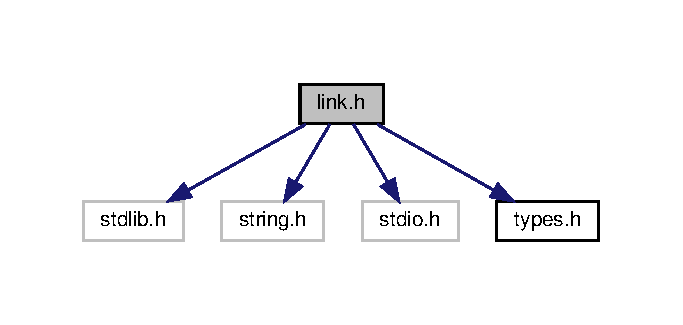
\includegraphics[width=328pt]{link_8h__incl}
\end{center}
\end{figure}
This graph shows which files directly or indirectly include this file\+:\nopagebreak
\begin{figure}[H]
\begin{center}
\leavevmode
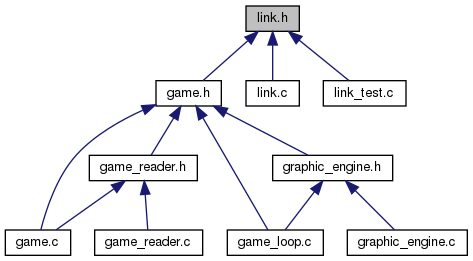
\includegraphics[width=350pt]{link_8h__dep__incl}
\end{center}
\end{figure}
\subsection*{Typedefs}
\begin{DoxyCompactItemize}
\item 
typedef struct \hyperlink{struct__Link}{\+\_\+\+Link} \hyperlink{link_8h_ae3b299941e67be6971bfd64a25505eff}{Link}
\end{DoxyCompactItemize}
\subsection*{Functions}
\begin{DoxyCompactItemize}
\item 
\hyperlink{link_8h_ae3b299941e67be6971bfd64a25505eff}{Link} $\ast$ \hyperlink{link_8h_aaf21d03943afcbed370ca720f972482c}{link\+\_\+create} ()
\begin{DoxyCompactList}\small\item\em crea un link \end{DoxyCompactList}\item 
void \hyperlink{link_8h_a117e4e5a82b23b805052d1eace34d068}{link\+\_\+destroy} (\hyperlink{link_8h_ae3b299941e67be6971bfd64a25505eff}{Link} $\ast$link)
\begin{DoxyCompactList}\small\item\em destruye y libera la memoria de un link \end{DoxyCompactList}\item 
\hyperlink{types_8h_a845e604fb28f7e3d97549da3448149d3}{Id} \hyperlink{link_8h_a2bbd320f995a72b2ea7ea639b1c81892}{link\+\_\+get\+\_\+id} (\hyperlink{link_8h_ae3b299941e67be6971bfd64a25505eff}{Link} $\ast$link)
\begin{DoxyCompactList}\small\item\em devuelve el Id de un link \end{DoxyCompactList}\item 
char $\ast$ \hyperlink{link_8h_a9747ee8201a323e112e67bdeacbc90d8}{link\+\_\+get\+\_\+name} (\hyperlink{link_8h_ae3b299941e67be6971bfd64a25505eff}{Link} $\ast$link)
\begin{DoxyCompactList}\small\item\em devuelve el Id de un link \end{DoxyCompactList}\item 
\hyperlink{types_8h_a845e604fb28f7e3d97549da3448149d3}{Id} \hyperlink{link_8h_a8b02c6629b52f2be8fa22c8f3f7466fe}{link\+\_\+get\+\_\+conection\+\_\+1} (\hyperlink{link_8h_ae3b299941e67be6971bfd64a25505eff}{Link} $\ast$link)
\begin{DoxyCompactList}\small\item\em el Id de la conexion 1 del link \end{DoxyCompactList}\item 
\hyperlink{types_8h_a845e604fb28f7e3d97549da3448149d3}{Id} \hyperlink{link_8h_ae49357746643a5e0786c6c1c843f0351}{link\+\_\+get\+\_\+conection\+\_\+2} (\hyperlink{link_8h_ae3b299941e67be6971bfd64a25505eff}{Link} $\ast$link)
\begin{DoxyCompactList}\small\item\em el Id de la conexion 2 del link \end{DoxyCompactList}\item 
\hyperlink{types_8h_a3e5b8192e7d9ffaf3542f1210aec18dd}{B\+O\+OL} \hyperlink{link_8h_af50c9578ed458d4ef4f4c85bdb60b3e1}{link\+\_\+get\+\_\+status} (\hyperlink{link_8h_ae3b299941e67be6971bfd64a25505eff}{Link} $\ast$link)
\begin{DoxyCompactList}\small\item\em comprueba si la conexion esta abierta o cerrada \end{DoxyCompactList}\item 
\hyperlink{types_8h_a32c27cc471df37f4fc818d65de0a56c4}{S\+T\+A\+T\+US} \hyperlink{link_8h_a3fd49fb1a3f19be4fc800ff07820cafb}{link\+\_\+set\+\_\+id} (\hyperlink{link_8h_ae3b299941e67be6971bfd64a25505eff}{Link} $\ast$link, \hyperlink{types_8h_a845e604fb28f7e3d97549da3448149d3}{Id} id)
\begin{DoxyCompactList}\small\item\em modifica el Id de un link \end{DoxyCompactList}\item 
\hyperlink{types_8h_a32c27cc471df37f4fc818d65de0a56c4}{S\+T\+A\+T\+US} \hyperlink{link_8h_a6c7a3bd7a856288c377edbcd045912e6}{link\+\_\+set\+\_\+name} (\hyperlink{link_8h_ae3b299941e67be6971bfd64a25505eff}{Link} $\ast$link, char $\ast$name)
\begin{DoxyCompactList}\small\item\em modifica el nombre de un link \end{DoxyCompactList}\item 
\hyperlink{types_8h_a32c27cc471df37f4fc818d65de0a56c4}{S\+T\+A\+T\+US} \hyperlink{link_8h_a93bfde2dd6d354dfca04cf0643317433}{link\+\_\+set\+\_\+conection} (\hyperlink{link_8h_ae3b299941e67be6971bfd64a25505eff}{Link} $\ast$link, \hyperlink{types_8h_a845e604fb28f7e3d97549da3448149d3}{Id} id1, \hyperlink{types_8h_a845e604fb28f7e3d97549da3448149d3}{Id} id2)
\begin{DoxyCompactList}\small\item\em modifica ela conexion de un link \end{DoxyCompactList}\item 
\hyperlink{types_8h_a32c27cc471df37f4fc818d65de0a56c4}{S\+T\+A\+T\+US} \hyperlink{link_8h_a9cd26b9d2d38b901380885e8ea7edec4}{link\+\_\+set\+\_\+status} (\hyperlink{link_8h_ae3b299941e67be6971bfd64a25505eff}{Link} $\ast$link, \hyperlink{types_8h_a3e5b8192e7d9ffaf3542f1210aec18dd}{B\+O\+OL} bool)
\begin{DoxyCompactList}\small\item\em modifica el estado de un link \end{DoxyCompactList}\item 
int \hyperlink{link_8h_ab5c45f8c1edc80d2f2dd73f5539d1951}{link\+\_\+print} (\hyperlink{link_8h_ae3b299941e67be6971bfd64a25505eff}{Link} $\ast$link)
\begin{DoxyCompactList}\small\item\em imprime un link \end{DoxyCompactList}\end{DoxyCompactItemize}


\subsection{Detailed Description}
En este fichero implementamos las funciones de link. 

\begin{DoxyAuthor}{Author}
Manuel Suarez, Saul Almazán, Álvaro Becerra, Rodrigo Lardiés 
\end{DoxyAuthor}
\begin{DoxyVersion}{Version}
1.\+0 
\end{DoxyVersion}
\begin{DoxyDate}{Date}
15/11/2018 
\end{DoxyDate}


\subsection{Typedef Documentation}
\mbox{\Hypertarget{link_8h_ae3b299941e67be6971bfd64a25505eff}\label{link_8h_ae3b299941e67be6971bfd64a25505eff}} 
\index{link.\+h@{link.\+h}!Link@{Link}}
\index{Link@{Link}!link.\+h@{link.\+h}}
\subsubsection{\texorpdfstring{Link}{Link}}
{\footnotesize\ttfamily typedef struct \hyperlink{struct__Link}{\+\_\+\+Link} \hyperlink{link_8h_ae3b299941e67be6971bfd64a25505eff}{Link}}

Estructura del link 

\subsection{Function Documentation}
\mbox{\Hypertarget{link_8h_aaf21d03943afcbed370ca720f972482c}\label{link_8h_aaf21d03943afcbed370ca720f972482c}} 
\index{link.\+h@{link.\+h}!link\+\_\+create@{link\+\_\+create}}
\index{link\+\_\+create@{link\+\_\+create}!link.\+h@{link.\+h}}
\subsubsection{\texorpdfstring{link\+\_\+create()}{link\_create()}}
{\footnotesize\ttfamily \hyperlink{link_8h_ae3b299941e67be6971bfd64a25505eff}{Link}$\ast$ link\+\_\+create (\begin{DoxyParamCaption}{ }\end{DoxyParamCaption})}



crea un link 

\begin{DoxyAuthor}{Author}
Manuel Suarez, Saul Almazán, Álvaro Becerra, Rodrigo Lardiés 
\end{DoxyAuthor}
\begin{DoxyDate}{Date}
15/11/2018 
\end{DoxyDate}
\begin{DoxyReturn}{Returns}
Link (El link que crea) 
\end{DoxyReturn}
\mbox{\Hypertarget{link_8h_a117e4e5a82b23b805052d1eace34d068}\label{link_8h_a117e4e5a82b23b805052d1eace34d068}} 
\index{link.\+h@{link.\+h}!link\+\_\+destroy@{link\+\_\+destroy}}
\index{link\+\_\+destroy@{link\+\_\+destroy}!link.\+h@{link.\+h}}
\subsubsection{\texorpdfstring{link\+\_\+destroy()}{link\_destroy()}}
{\footnotesize\ttfamily void link\+\_\+destroy (\begin{DoxyParamCaption}\item[{\hyperlink{link_8h_ae3b299941e67be6971bfd64a25505eff}{Link} $\ast$}]{link }\end{DoxyParamCaption})}



destruye y libera la memoria de un link 

\begin{DoxyAuthor}{Author}
Manuel Suarez, Saul Almazán, Álvaro Becerra, Rodrigo Lardiés 
\end{DoxyAuthor}
\begin{DoxyDate}{Date}
15/11/2018 
\end{DoxyDate}

\begin{DoxyParams}{Parameters}
{\em link} & (link a destruir) \\
\hline
\end{DoxyParams}
\begin{DoxyReturn}{Returns}
void (No devuelve nada) 
\end{DoxyReturn}
\mbox{\Hypertarget{link_8h_a8b02c6629b52f2be8fa22c8f3f7466fe}\label{link_8h_a8b02c6629b52f2be8fa22c8f3f7466fe}} 
\index{link.\+h@{link.\+h}!link\+\_\+get\+\_\+conection\+\_\+1@{link\+\_\+get\+\_\+conection\+\_\+1}}
\index{link\+\_\+get\+\_\+conection\+\_\+1@{link\+\_\+get\+\_\+conection\+\_\+1}!link.\+h@{link.\+h}}
\subsubsection{\texorpdfstring{link\+\_\+get\+\_\+conection\+\_\+1()}{link\_get\_conection\_1()}}
{\footnotesize\ttfamily \hyperlink{types_8h_a845e604fb28f7e3d97549da3448149d3}{Id} link\+\_\+get\+\_\+conection\+\_\+1 (\begin{DoxyParamCaption}\item[{\hyperlink{link_8h_ae3b299941e67be6971bfd64a25505eff}{Link} $\ast$}]{link }\end{DoxyParamCaption})}



el Id de la conexion 1 del link 

\begin{DoxyAuthor}{Author}
Manuel Suarez, Saul Almazán, Álvaro Becerra, Rodrigo Lardiés 
\end{DoxyAuthor}
\begin{DoxyDate}{Date}
15/11/2018 
\end{DoxyDate}

\begin{DoxyParams}{Parameters}
{\em link} & (link a usar) \\
\hline
\end{DoxyParams}
\begin{DoxyReturn}{Returns}
(Id de la conexion)
\end{DoxyReturn}
\begin{DoxyAuthor}{Author}
Manuel Suarez, Saul Almazán, Álvaro Becerra, Rodrigo Lardiés 
\end{DoxyAuthor}
\begin{DoxyDate}{Date}
15/11/2018 
\end{DoxyDate}

\begin{DoxyParams}{Parameters}
{\em link} & (link a usar) \\
\hline
\end{DoxyParams}
\begin{DoxyReturn}{Returns}
Id (Id de la conexion) 
\end{DoxyReturn}
\mbox{\Hypertarget{link_8h_ae49357746643a5e0786c6c1c843f0351}\label{link_8h_ae49357746643a5e0786c6c1c843f0351}} 
\index{link.\+h@{link.\+h}!link\+\_\+get\+\_\+conection\+\_\+2@{link\+\_\+get\+\_\+conection\+\_\+2}}
\index{link\+\_\+get\+\_\+conection\+\_\+2@{link\+\_\+get\+\_\+conection\+\_\+2}!link.\+h@{link.\+h}}
\subsubsection{\texorpdfstring{link\+\_\+get\+\_\+conection\+\_\+2()}{link\_get\_conection\_2()}}
{\footnotesize\ttfamily \hyperlink{types_8h_a845e604fb28f7e3d97549da3448149d3}{Id} link\+\_\+get\+\_\+conection\+\_\+2 (\begin{DoxyParamCaption}\item[{\hyperlink{link_8h_ae3b299941e67be6971bfd64a25505eff}{Link} $\ast$}]{link }\end{DoxyParamCaption})}



el Id de la conexion 2 del link 

\begin{DoxyAuthor}{Author}
Manuel Suarez, Saul Almazán, Álvaro Becerra, Rodrigo Lardiés 
\end{DoxyAuthor}
\begin{DoxyDate}{Date}
15/11/2018 
\end{DoxyDate}

\begin{DoxyParams}{Parameters}
{\em link} & (link a usar) \\
\hline
\end{DoxyParams}
\begin{DoxyReturn}{Returns}
Id (Id de la conexion) 
\end{DoxyReturn}
\mbox{\Hypertarget{link_8h_a2bbd320f995a72b2ea7ea639b1c81892}\label{link_8h_a2bbd320f995a72b2ea7ea639b1c81892}} 
\index{link.\+h@{link.\+h}!link\+\_\+get\+\_\+id@{link\+\_\+get\+\_\+id}}
\index{link\+\_\+get\+\_\+id@{link\+\_\+get\+\_\+id}!link.\+h@{link.\+h}}
\subsubsection{\texorpdfstring{link\+\_\+get\+\_\+id()}{link\_get\_id()}}
{\footnotesize\ttfamily \hyperlink{types_8h_a845e604fb28f7e3d97549da3448149d3}{Id} link\+\_\+get\+\_\+id (\begin{DoxyParamCaption}\item[{\hyperlink{link_8h_ae3b299941e67be6971bfd64a25505eff}{Link} $\ast$}]{link }\end{DoxyParamCaption})}



devuelve el Id de un link 

\begin{DoxyAuthor}{Author}
Manuel Suarez, Saul Almazán, Álvaro Becerra, Rodrigo Lardiés 
\end{DoxyAuthor}
\begin{DoxyDate}{Date}
15/11/2018 
\end{DoxyDate}

\begin{DoxyParams}{Parameters}
{\em link} & (link a usar) \\
\hline
\end{DoxyParams}
\begin{DoxyReturn}{Returns}
Id (Id del link) 
\end{DoxyReturn}
\mbox{\Hypertarget{link_8h_a9747ee8201a323e112e67bdeacbc90d8}\label{link_8h_a9747ee8201a323e112e67bdeacbc90d8}} 
\index{link.\+h@{link.\+h}!link\+\_\+get\+\_\+name@{link\+\_\+get\+\_\+name}}
\index{link\+\_\+get\+\_\+name@{link\+\_\+get\+\_\+name}!link.\+h@{link.\+h}}
\subsubsection{\texorpdfstring{link\+\_\+get\+\_\+name()}{link\_get\_name()}}
{\footnotesize\ttfamily char$\ast$ link\+\_\+get\+\_\+name (\begin{DoxyParamCaption}\item[{\hyperlink{link_8h_ae3b299941e67be6971bfd64a25505eff}{Link} $\ast$}]{link }\end{DoxyParamCaption})}



devuelve el Id de un link 

\begin{DoxyAuthor}{Author}
Manuel Suarez, Saul Almazán, Álvaro Becerra, Rodrigo Lardiés 
\end{DoxyAuthor}
\begin{DoxyDate}{Date}
15/11/2018 
\end{DoxyDate}

\begin{DoxyParams}{Parameters}
{\em link} & (link a usar) \\
\hline
\end{DoxyParams}
\begin{DoxyReturn}{Returns}
char (nombre del link) 
\end{DoxyReturn}
\mbox{\Hypertarget{link_8h_af50c9578ed458d4ef4f4c85bdb60b3e1}\label{link_8h_af50c9578ed458d4ef4f4c85bdb60b3e1}} 
\index{link.\+h@{link.\+h}!link\+\_\+get\+\_\+status@{link\+\_\+get\+\_\+status}}
\index{link\+\_\+get\+\_\+status@{link\+\_\+get\+\_\+status}!link.\+h@{link.\+h}}
\subsubsection{\texorpdfstring{link\+\_\+get\+\_\+status()}{link\_get\_status()}}
{\footnotesize\ttfamily \hyperlink{types_8h_a3e5b8192e7d9ffaf3542f1210aec18dd}{B\+O\+OL} link\+\_\+get\+\_\+status (\begin{DoxyParamCaption}\item[{\hyperlink{link_8h_ae3b299941e67be6971bfd64a25505eff}{Link} $\ast$}]{link }\end{DoxyParamCaption})}



comprueba si la conexion esta abierta o cerrada 

\begin{DoxyAuthor}{Author}
Manuel Suarez, Saul Almazán, Álvaro Becerra, Rodrigo Lardiés 
\end{DoxyAuthor}
\begin{DoxyDate}{Date}
15/11/2018 
\end{DoxyDate}

\begin{DoxyParams}{Parameters}
{\em link} & (link a usar) \\
\hline
\end{DoxyParams}
\begin{DoxyReturn}{Returns}
B\+O\+OL (T\+R\+UE o F\+A\+L\+SE dependiendo de si la conexion esta abierta o cerrada) 
\end{DoxyReturn}
\mbox{\Hypertarget{link_8h_ab5c45f8c1edc80d2f2dd73f5539d1951}\label{link_8h_ab5c45f8c1edc80d2f2dd73f5539d1951}} 
\index{link.\+h@{link.\+h}!link\+\_\+print@{link\+\_\+print}}
\index{link\+\_\+print@{link\+\_\+print}!link.\+h@{link.\+h}}
\subsubsection{\texorpdfstring{link\+\_\+print()}{link\_print()}}
{\footnotesize\ttfamily int link\+\_\+print (\begin{DoxyParamCaption}\item[{\hyperlink{link_8h_ae3b299941e67be6971bfd64a25505eff}{Link} $\ast$}]{link }\end{DoxyParamCaption})}



imprime un link 

\begin{DoxyAuthor}{Author}
Manuel Suarez, Saul Almazán, Álvaro Becerra, Rodrigo Lardiés 
\end{DoxyAuthor}
\begin{DoxyDate}{Date}
15/11/2018 
\end{DoxyDate}

\begin{DoxyParams}{Parameters}
{\em link} & (link a modificar) \\
\hline
\end{DoxyParams}
\begin{DoxyReturn}{Returns}
int (-\/1 si no se ha realizado con exito) 
\end{DoxyReturn}
\mbox{\Hypertarget{link_8h_a93bfde2dd6d354dfca04cf0643317433}\label{link_8h_a93bfde2dd6d354dfca04cf0643317433}} 
\index{link.\+h@{link.\+h}!link\+\_\+set\+\_\+conection@{link\+\_\+set\+\_\+conection}}
\index{link\+\_\+set\+\_\+conection@{link\+\_\+set\+\_\+conection}!link.\+h@{link.\+h}}
\subsubsection{\texorpdfstring{link\+\_\+set\+\_\+conection()}{link\_set\_conection()}}
{\footnotesize\ttfamily \hyperlink{types_8h_a32c27cc471df37f4fc818d65de0a56c4}{S\+T\+A\+T\+US} link\+\_\+set\+\_\+conection (\begin{DoxyParamCaption}\item[{\hyperlink{link_8h_ae3b299941e67be6971bfd64a25505eff}{Link} $\ast$}]{link,  }\item[{\hyperlink{types_8h_a845e604fb28f7e3d97549da3448149d3}{Id}}]{id1,  }\item[{\hyperlink{types_8h_a845e604fb28f7e3d97549da3448149d3}{Id}}]{id2 }\end{DoxyParamCaption})}



modifica ela conexion de un link 

\begin{DoxyAuthor}{Author}
Manuel Suarez, Saul Almazán, Álvaro Becerra, Rodrigo Lardiés 
\end{DoxyAuthor}
\begin{DoxyDate}{Date}
15/11/2018 
\end{DoxyDate}

\begin{DoxyParams}{Parameters}
{\em link} & (link a modificar) \\
\hline
{\em id1} & (Nuevo id) \\
\hline
{\em id2} & (Nuevo Id) \\
\hline
\end{DoxyParams}
\begin{DoxyReturn}{Returns}
S\+T\+A\+T\+US (OK si se ha realizado correctamente o E\+R\+R\+OR de lo contrario)
\end{DoxyReturn}
\begin{DoxyAuthor}{Author}
Manuel Suarez, Saul Almazán, Álvaro Becerra, Rodrigo Lardiés 
\end{DoxyAuthor}
\begin{DoxyDate}{Date}
15/11/2018 
\end{DoxyDate}

\begin{DoxyParams}{Parameters}
{\em link} & (link a modificar) \\
\hline
{\em id1} & (Nuevo id1) \\
\hline
{\em id2} & (Nuevo Id2) \\
\hline
\end{DoxyParams}
\begin{DoxyReturn}{Returns}
S\+T\+A\+T\+US (OK si se ha realizado correctamente o E\+R\+R\+OR de lo contrario) 
\end{DoxyReturn}
\mbox{\Hypertarget{link_8h_a3fd49fb1a3f19be4fc800ff07820cafb}\label{link_8h_a3fd49fb1a3f19be4fc800ff07820cafb}} 
\index{link.\+h@{link.\+h}!link\+\_\+set\+\_\+id@{link\+\_\+set\+\_\+id}}
\index{link\+\_\+set\+\_\+id@{link\+\_\+set\+\_\+id}!link.\+h@{link.\+h}}
\subsubsection{\texorpdfstring{link\+\_\+set\+\_\+id()}{link\_set\_id()}}
{\footnotesize\ttfamily \hyperlink{types_8h_a32c27cc471df37f4fc818d65de0a56c4}{S\+T\+A\+T\+US} link\+\_\+set\+\_\+id (\begin{DoxyParamCaption}\item[{\hyperlink{link_8h_ae3b299941e67be6971bfd64a25505eff}{Link} $\ast$}]{link,  }\item[{\hyperlink{types_8h_a845e604fb28f7e3d97549da3448149d3}{Id}}]{id }\end{DoxyParamCaption})}



modifica el Id de un link 

\begin{DoxyAuthor}{Author}
Manuel Suarez, Saul Almazán, Álvaro Becerra, Rodrigo Lardiés 
\end{DoxyAuthor}
\begin{DoxyDate}{Date}
15/11/2018 
\end{DoxyDate}

\begin{DoxyParams}{Parameters}
{\em link} & (link a modificar) \\
\hline
{\em id} & (Nuevo Id) \\
\hline
\end{DoxyParams}
\begin{DoxyReturn}{Returns}
S\+T\+A\+T\+US (OK si se ha realizado correctamente o E\+R\+R\+OR de lo contrario) 
\end{DoxyReturn}
\mbox{\Hypertarget{link_8h_a6c7a3bd7a856288c377edbcd045912e6}\label{link_8h_a6c7a3bd7a856288c377edbcd045912e6}} 
\index{link.\+h@{link.\+h}!link\+\_\+set\+\_\+name@{link\+\_\+set\+\_\+name}}
\index{link\+\_\+set\+\_\+name@{link\+\_\+set\+\_\+name}!link.\+h@{link.\+h}}
\subsubsection{\texorpdfstring{link\+\_\+set\+\_\+name()}{link\_set\_name()}}
{\footnotesize\ttfamily \hyperlink{types_8h_a32c27cc471df37f4fc818d65de0a56c4}{S\+T\+A\+T\+US} link\+\_\+set\+\_\+name (\begin{DoxyParamCaption}\item[{\hyperlink{link_8h_ae3b299941e67be6971bfd64a25505eff}{Link} $\ast$}]{link,  }\item[{char $\ast$}]{name }\end{DoxyParamCaption})}



modifica el nombre de un link 

\begin{DoxyAuthor}{Author}
Manuel Suarez, Saul Almazán, Álvaro Becerra, Rodrigo Lardiés 
\end{DoxyAuthor}
\begin{DoxyDate}{Date}
15/11/2018 
\end{DoxyDate}

\begin{DoxyParams}{Parameters}
{\em link} & (link a modificar) \\
\hline
{\em name} & (Nuevo nombre) \\
\hline
\end{DoxyParams}
\begin{DoxyReturn}{Returns}
S\+T\+A\+T\+US (OK si se ha realizado correctamente o E\+R\+R\+OR de lo contrario) 
\end{DoxyReturn}
\mbox{\Hypertarget{link_8h_a9cd26b9d2d38b901380885e8ea7edec4}\label{link_8h_a9cd26b9d2d38b901380885e8ea7edec4}} 
\index{link.\+h@{link.\+h}!link\+\_\+set\+\_\+status@{link\+\_\+set\+\_\+status}}
\index{link\+\_\+set\+\_\+status@{link\+\_\+set\+\_\+status}!link.\+h@{link.\+h}}
\subsubsection{\texorpdfstring{link\+\_\+set\+\_\+status()}{link\_set\_status()}}
{\footnotesize\ttfamily \hyperlink{types_8h_a32c27cc471df37f4fc818d65de0a56c4}{S\+T\+A\+T\+US} link\+\_\+set\+\_\+status (\begin{DoxyParamCaption}\item[{\hyperlink{link_8h_ae3b299941e67be6971bfd64a25505eff}{Link} $\ast$}]{link,  }\item[{\hyperlink{types_8h_a3e5b8192e7d9ffaf3542f1210aec18dd}{B\+O\+OL}}]{bool }\end{DoxyParamCaption})}



modifica el estado de un link 

\begin{DoxyAuthor}{Author}
Manuel Suarez, Saul Almazán, Álvaro Becerra, Rodrigo Lardiés 
\end{DoxyAuthor}
\begin{DoxyDate}{Date}
15/11/2018 
\end{DoxyDate}

\begin{DoxyParams}{Parameters}
{\em link} & (link a modificar) \\
\hline
{\em bool} & (Nuevo estado) \\
\hline
\end{DoxyParams}
\begin{DoxyReturn}{Returns}
S\+T\+A\+T\+US (OK si se ha realizado correctamente o E\+R\+R\+OR de lo contrario) 
\end{DoxyReturn}

\hypertarget{link__test_8h}{}\section{include/link\+\_\+test.h File Reference}
\label{link__test_8h}\index{include/link\+\_\+test.\+h@{include/link\+\_\+test.\+h}}


Prueba del modulo link.  


This graph shows which files directly or indirectly include this file\+:
% FIG 0
\subsection*{Functions}
\begin{DoxyCompactItemize}
\item 
void \hyperlink{link__test_8h_a82c5ee441ad22caad8272212a9e9cc26}{test1\+\_\+link\+\_\+create} ()
\item 
void \hyperlink{link__test_8h_ae0e478a0540bed26befc071591e3ff6c}{test1\+\_\+link\+\_\+set\+\_\+name} ()
\item 
void \hyperlink{link__test_8h_aa66c1e991620a5a758ba6e4d6b4a8b73}{test2\+\_\+link\+\_\+set\+\_\+name} ()
\item 
void \hyperlink{link__test_8h_a8396e33f601deb52c940cb89cd7c6bfe}{test3\+\_\+link\+\_\+set\+\_\+name} ()
\item 
void \hyperlink{link__test_8h_ac2b67785fdf6bb85af93e985af9ee3f2}{test1\+\_\+link\+\_\+set\+\_\+id} ()
\item 
void \hyperlink{link__test_8h_a2f107a28c71f764c8091747f48eaec3f}{test2\+\_\+link\+\_\+set\+\_\+id} ()
\item 
void \hyperlink{link__test_8h_a8c70e0dc87dfcbfff2e690fbee50ebf2}{test1\+\_\+link\+\_\+set\+\_\+conection} ()
\item 
void \hyperlink{link__test_8h_a1f9f58ce35b89b92b33d51e5f7a22156}{test2\+\_\+link\+\_\+set\+\_\+conection} ()
\item 
void \hyperlink{link__test_8h_a3b39fdba0c3c967716572bfb01beec27}{test1\+\_\+link\+\_\+set\+\_\+status} ()
\item 
void \hyperlink{link__test_8h_a315ea19cd24434d2153b5df9f372a561}{test2\+\_\+link\+\_\+set\+\_\+status} ()
\item 
void \hyperlink{link__test_8h_a044128db00a5cc385d7157dea8bdf3c3}{test1\+\_\+link\+\_\+get\+\_\+name} ()
\item 
void \hyperlink{link__test_8h_a4efc6cfcdc210e2803f9d285734c571e}{test2\+\_\+link\+\_\+get\+\_\+name} ()
\item 
void \hyperlink{link__test_8h_a19c70f79fd51d123173f7aaf6ae50bf8}{test1\+\_\+link\+\_\+get\+\_\+id} ()
\item 
void \hyperlink{link__test_8h_a0f967a1782dd7264e73ad428d22d125d}{test2\+\_\+link\+\_\+get\+\_\+id} ()
\item 
void \hyperlink{link__test_8h_acc0691ef1025561d539b2c212ffbcc24}{test1\+\_\+link\+\_\+get\+\_\+conection\+\_\+1} ()
\item 
void \hyperlink{link__test_8h_a79d95fe7b7d20331545c527a26b18a62}{test2\+\_\+link\+\_\+get\+\_\+conection\+\_\+1} ()
\item 
void \hyperlink{link__test_8h_abe6d5eddefa0ccab66ccf641da6319b1}{test1\+\_\+link\+\_\+get\+\_\+conection\+\_\+2} ()
\item 
void \hyperlink{link__test_8h_a0a102f4a6a5fcc2026a75fb6675241d0}{test2\+\_\+link\+\_\+get\+\_\+conection\+\_\+2} ()
\item 
void \hyperlink{link__test_8h_a9f7bf73b9398d551c64f6c845e9e1560}{test1\+\_\+link\+\_\+get\+\_\+status} ()
\item 
void \hyperlink{link__test_8h_a7d1062febd832b21e69df5f071425b4c}{test2\+\_\+link\+\_\+get\+\_\+status} ()
\end{DoxyCompactItemize}


\subsection{Detailed Description}
Prueba del modulo link. 

\begin{DoxyAuthor}{Author}
Manuel Suarez, Saul Almazán, Álvaro Becerra, Rodrigo Lardiés 
\end{DoxyAuthor}
\begin{DoxyVersion}{Version}
1.\+0 
\end{DoxyVersion}
\begin{DoxyDate}{Date}
12-\/11-\/2018 
\end{DoxyDate}


\subsection{Function Documentation}
\mbox{\Hypertarget{link__test_8h_a82c5ee441ad22caad8272212a9e9cc26}\label{link__test_8h_a82c5ee441ad22caad8272212a9e9cc26}} 
\index{link\+\_\+test.\+h@{link\+\_\+test.\+h}!test1\+\_\+link\+\_\+create@{test1\+\_\+link\+\_\+create}}
\index{test1\+\_\+link\+\_\+create@{test1\+\_\+link\+\_\+create}!link\+\_\+test.\+h@{link\+\_\+test.\+h}}
\subsubsection{\texorpdfstring{test1\+\_\+link\+\_\+create()}{test1\_link\_create()}}
{\footnotesize\ttfamily void test1\+\_\+link\+\_\+create (\begin{DoxyParamCaption}{ }\end{DoxyParamCaption})}

\begin{DoxyRefDesc}{Test}
\item[\hyperlink{test__test000184}{Test}]Prueba la función de creación de un link \end{DoxyRefDesc}
\begin{DoxyPrecond}{Precondition}
Nada 
\end{DoxyPrecond}
\begin{DoxyPostcond}{Postcondition}
Un puntero no nulo al link creado
\end{DoxyPostcond}
\begin{DoxyRefDesc}{Test}
\item[\hyperlink{test__test000027}{Test}]Prueba la función de creación de un link \end{DoxyRefDesc}
\begin{DoxyPrecond}{Precondition}
Nada 
\end{DoxyPrecond}
\begin{DoxyPostcond}{Postcondition}
Un puntero no nulo al link creado 
\end{DoxyPostcond}
\mbox{\Hypertarget{link__test_8h_acc0691ef1025561d539b2c212ffbcc24}\label{link__test_8h_acc0691ef1025561d539b2c212ffbcc24}} 
\index{link\+\_\+test.\+h@{link\+\_\+test.\+h}!test1\+\_\+link\+\_\+get\+\_\+conection\+\_\+1@{test1\+\_\+link\+\_\+get\+\_\+conection\+\_\+1}}
\index{test1\+\_\+link\+\_\+get\+\_\+conection\+\_\+1@{test1\+\_\+link\+\_\+get\+\_\+conection\+\_\+1}!link\+\_\+test.\+h@{link\+\_\+test.\+h}}
\subsubsection{\texorpdfstring{test1\+\_\+link\+\_\+get\+\_\+conection\+\_\+1()}{test1\_link\_get\_conection\_1()}}
{\footnotesize\ttfamily void test1\+\_\+link\+\_\+get\+\_\+conection\+\_\+1 (\begin{DoxyParamCaption}{ }\end{DoxyParamCaption})}

\begin{DoxyRefDesc}{Test}
\item[\hyperlink{test__test000198}{Test}]Prueba la función para obtener el id 1 de un link \end{DoxyRefDesc}
\begin{DoxyPrecond}{Precondition}
El link tiene un id establecido 
\end{DoxyPrecond}
\begin{DoxyPostcond}{Postcondition}
La salida debe ser id=1
\end{DoxyPostcond}
\begin{DoxyRefDesc}{Test}
\item[\hyperlink{test__test000041}{Test}]Prueba la función para obtener el id 1 de un link \end{DoxyRefDesc}
\begin{DoxyPrecond}{Precondition}
El link tiene un id establecido 
\end{DoxyPrecond}
\begin{DoxyPostcond}{Postcondition}
La salida debe ser id=1 
\end{DoxyPostcond}
\mbox{\Hypertarget{link__test_8h_abe6d5eddefa0ccab66ccf641da6319b1}\label{link__test_8h_abe6d5eddefa0ccab66ccf641da6319b1}} 
\index{link\+\_\+test.\+h@{link\+\_\+test.\+h}!test1\+\_\+link\+\_\+get\+\_\+conection\+\_\+2@{test1\+\_\+link\+\_\+get\+\_\+conection\+\_\+2}}
\index{test1\+\_\+link\+\_\+get\+\_\+conection\+\_\+2@{test1\+\_\+link\+\_\+get\+\_\+conection\+\_\+2}!link\+\_\+test.\+h@{link\+\_\+test.\+h}}
\subsubsection{\texorpdfstring{test1\+\_\+link\+\_\+get\+\_\+conection\+\_\+2()}{test1\_link\_get\_conection\_2()}}
{\footnotesize\ttfamily void test1\+\_\+link\+\_\+get\+\_\+conection\+\_\+2 (\begin{DoxyParamCaption}{ }\end{DoxyParamCaption})}

\begin{DoxyRefDesc}{Test}
\item[\hyperlink{test__test000200}{Test}]Prueba la función para obtener el id 2 de un link \end{DoxyRefDesc}
\begin{DoxyPrecond}{Precondition}
El link tiene un id establecido 
\end{DoxyPrecond}
\begin{DoxyPostcond}{Postcondition}
La salida debe ser id=1
\end{DoxyPostcond}
\begin{DoxyRefDesc}{Test}
\item[\hyperlink{test__test000043}{Test}]Prueba la función para obtener el id 2 de un link \end{DoxyRefDesc}
\begin{DoxyPrecond}{Precondition}
El link tiene un id establecido 
\end{DoxyPrecond}
\begin{DoxyPostcond}{Postcondition}
La salida debe ser id=1 
\end{DoxyPostcond}
\mbox{\Hypertarget{link__test_8h_a19c70f79fd51d123173f7aaf6ae50bf8}\label{link__test_8h_a19c70f79fd51d123173f7aaf6ae50bf8}} 
\index{link\+\_\+test.\+h@{link\+\_\+test.\+h}!test1\+\_\+link\+\_\+get\+\_\+id@{test1\+\_\+link\+\_\+get\+\_\+id}}
\index{test1\+\_\+link\+\_\+get\+\_\+id@{test1\+\_\+link\+\_\+get\+\_\+id}!link\+\_\+test.\+h@{link\+\_\+test.\+h}}
\subsubsection{\texorpdfstring{test1\+\_\+link\+\_\+get\+\_\+id()}{test1\_link\_get\_id()}}
{\footnotesize\ttfamily void test1\+\_\+link\+\_\+get\+\_\+id (\begin{DoxyParamCaption}{ }\end{DoxyParamCaption})}

\begin{DoxyRefDesc}{Test}
\item[\hyperlink{test__test000196}{Test}]Prueba la función para obtener el id de un link \end{DoxyRefDesc}
\begin{DoxyPrecond}{Precondition}
El link tiene un id establecido 
\end{DoxyPrecond}
\begin{DoxyPostcond}{Postcondition}
La salida debe ser id=1
\end{DoxyPostcond}
\begin{DoxyRefDesc}{Test}
\item[\hyperlink{test__test000039}{Test}]Prueba la función para obtener el id de un link \end{DoxyRefDesc}
\begin{DoxyPrecond}{Precondition}
El link tiene un id establecido 
\end{DoxyPrecond}
\begin{DoxyPostcond}{Postcondition}
La salida debe ser id=1 
\end{DoxyPostcond}
\mbox{\Hypertarget{link__test_8h_a044128db00a5cc385d7157dea8bdf3c3}\label{link__test_8h_a044128db00a5cc385d7157dea8bdf3c3}} 
\index{link\+\_\+test.\+h@{link\+\_\+test.\+h}!test1\+\_\+link\+\_\+get\+\_\+name@{test1\+\_\+link\+\_\+get\+\_\+name}}
\index{test1\+\_\+link\+\_\+get\+\_\+name@{test1\+\_\+link\+\_\+get\+\_\+name}!link\+\_\+test.\+h@{link\+\_\+test.\+h}}
\subsubsection{\texorpdfstring{test1\+\_\+link\+\_\+get\+\_\+name()}{test1\_link\_get\_name()}}
{\footnotesize\ttfamily void test1\+\_\+link\+\_\+get\+\_\+name (\begin{DoxyParamCaption}{ }\end{DoxyParamCaption})}

\begin{DoxyRefDesc}{Test}
\item[\hyperlink{test__test000194}{Test}]Prueba la función para obtener el nombre de un link \end{DoxyRefDesc}
\begin{DoxyPrecond}{Precondition}
El link tiene un nombre establecido 
\end{DoxyPrecond}
\begin{DoxyPostcond}{Postcondition}
La salida debe ser una comparación de cadenas igual a 0
\end{DoxyPostcond}
\begin{DoxyRefDesc}{Test}
\item[\hyperlink{test__test000037}{Test}]Prueba la función para obtener el nombre de un link \end{DoxyRefDesc}
\begin{DoxyPrecond}{Precondition}
El link tiene un nombre establecido 
\end{DoxyPrecond}
\begin{DoxyPostcond}{Postcondition}
La salida debe ser una comparación de cadenas igual a 0 
\end{DoxyPostcond}
\mbox{\Hypertarget{link__test_8h_a9f7bf73b9398d551c64f6c845e9e1560}\label{link__test_8h_a9f7bf73b9398d551c64f6c845e9e1560}} 
\index{link\+\_\+test.\+h@{link\+\_\+test.\+h}!test1\+\_\+link\+\_\+get\+\_\+status@{test1\+\_\+link\+\_\+get\+\_\+status}}
\index{test1\+\_\+link\+\_\+get\+\_\+status@{test1\+\_\+link\+\_\+get\+\_\+status}!link\+\_\+test.\+h@{link\+\_\+test.\+h}}
\subsubsection{\texorpdfstring{test1\+\_\+link\+\_\+get\+\_\+status()}{test1\_link\_get\_status()}}
{\footnotesize\ttfamily void test1\+\_\+link\+\_\+get\+\_\+status (\begin{DoxyParamCaption}{ }\end{DoxyParamCaption})}

\begin{DoxyRefDesc}{Test}
\item[\hyperlink{test__test000202}{Test}]Prueba la función para saber el estado de un link \end{DoxyRefDesc}
\begin{DoxyPrecond}{Precondition}
link con un estado asignado 
\end{DoxyPrecond}
\begin{DoxyPostcond}{Postcondition}
La salida debe ser T\+R\+UE
\end{DoxyPostcond}
\begin{DoxyRefDesc}{Test}
\item[\hyperlink{test__test000045}{Test}]Prueba la función para saber el estado de un link \end{DoxyRefDesc}
\begin{DoxyPrecond}{Precondition}
link con un estado asignado 
\end{DoxyPrecond}
\begin{DoxyPostcond}{Postcondition}
La salida debe ser T\+R\+UE 
\end{DoxyPostcond}
\mbox{\Hypertarget{link__test_8h_a8c70e0dc87dfcbfff2e690fbee50ebf2}\label{link__test_8h_a8c70e0dc87dfcbfff2e690fbee50ebf2}} 
\index{link\+\_\+test.\+h@{link\+\_\+test.\+h}!test1\+\_\+link\+\_\+set\+\_\+conection@{test1\+\_\+link\+\_\+set\+\_\+conection}}
\index{test1\+\_\+link\+\_\+set\+\_\+conection@{test1\+\_\+link\+\_\+set\+\_\+conection}!link\+\_\+test.\+h@{link\+\_\+test.\+h}}
\subsubsection{\texorpdfstring{test1\+\_\+link\+\_\+set\+\_\+conection()}{test1\_link\_set\_conection()}}
{\footnotesize\ttfamily void test1\+\_\+link\+\_\+set\+\_\+conection (\begin{DoxyParamCaption}{ }\end{DoxyParamCaption})}

\begin{DoxyRefDesc}{Test}
\item[\hyperlink{test__test000190}{Test}]Prueba la función para establecer la conexion de un link \end{DoxyRefDesc}
\begin{DoxyPrecond}{Precondition}
ids que establecer al link 
\end{DoxyPrecond}
\begin{DoxyPostcond}{Postcondition}
La salida debe ser OK
\end{DoxyPostcond}
\begin{DoxyRefDesc}{Test}
\item[\hyperlink{test__test000033}{Test}]Prueba la función para establecer la conexion de un link \end{DoxyRefDesc}
\begin{DoxyPrecond}{Precondition}
ids que establecer al link 
\end{DoxyPrecond}
\begin{DoxyPostcond}{Postcondition}
La salida debe ser OK 
\end{DoxyPostcond}
\mbox{\Hypertarget{link__test_8h_ac2b67785fdf6bb85af93e985af9ee3f2}\label{link__test_8h_ac2b67785fdf6bb85af93e985af9ee3f2}} 
\index{link\+\_\+test.\+h@{link\+\_\+test.\+h}!test1\+\_\+link\+\_\+set\+\_\+id@{test1\+\_\+link\+\_\+set\+\_\+id}}
\index{test1\+\_\+link\+\_\+set\+\_\+id@{test1\+\_\+link\+\_\+set\+\_\+id}!link\+\_\+test.\+h@{link\+\_\+test.\+h}}
\subsubsection{\texorpdfstring{test1\+\_\+link\+\_\+set\+\_\+id()}{test1\_link\_set\_id()}}
{\footnotesize\ttfamily void test1\+\_\+link\+\_\+set\+\_\+id (\begin{DoxyParamCaption}{ }\end{DoxyParamCaption})}

\begin{DoxyRefDesc}{Test}
\item[\hyperlink{test__test000188}{Test}]Prueba la función para establecer el id de un link \end{DoxyRefDesc}
\begin{DoxyPrecond}{Precondition}
id que establecer al link 
\end{DoxyPrecond}
\begin{DoxyPostcond}{Postcondition}
La salida debe ser OK
\end{DoxyPostcond}
\begin{DoxyRefDesc}{Test}
\item[\hyperlink{test__test000031}{Test}]Prueba la función para establecer el id de un link \end{DoxyRefDesc}
\begin{DoxyPrecond}{Precondition}
id que establecer al link 
\end{DoxyPrecond}
\begin{DoxyPostcond}{Postcondition}
La salida debe ser OK 
\end{DoxyPostcond}
\mbox{\Hypertarget{link__test_8h_ae0e478a0540bed26befc071591e3ff6c}\label{link__test_8h_ae0e478a0540bed26befc071591e3ff6c}} 
\index{link\+\_\+test.\+h@{link\+\_\+test.\+h}!test1\+\_\+link\+\_\+set\+\_\+name@{test1\+\_\+link\+\_\+set\+\_\+name}}
\index{test1\+\_\+link\+\_\+set\+\_\+name@{test1\+\_\+link\+\_\+set\+\_\+name}!link\+\_\+test.\+h@{link\+\_\+test.\+h}}
\subsubsection{\texorpdfstring{test1\+\_\+link\+\_\+set\+\_\+name()}{test1\_link\_set\_name()}}
{\footnotesize\ttfamily void test1\+\_\+link\+\_\+set\+\_\+name (\begin{DoxyParamCaption}{ }\end{DoxyParamCaption})}

\begin{DoxyRefDesc}{Test}
\item[\hyperlink{test__test000185}{Test}]Prueba la función para establecer el nombre de un link \end{DoxyRefDesc}
\begin{DoxyPrecond}{Precondition}
Nombre que establecer al link 
\end{DoxyPrecond}
\begin{DoxyPostcond}{Postcondition}
La salida debe ser OK
\end{DoxyPostcond}
\begin{DoxyRefDesc}{Test}
\item[\hyperlink{test__test000028}{Test}]Prueba la función para establecer el nombre de un link \end{DoxyRefDesc}
\begin{DoxyPrecond}{Precondition}
Nombre que establecer al link 
\end{DoxyPrecond}
\begin{DoxyPostcond}{Postcondition}
La salida debe ser OK 
\end{DoxyPostcond}
\mbox{\Hypertarget{link__test_8h_a3b39fdba0c3c967716572bfb01beec27}\label{link__test_8h_a3b39fdba0c3c967716572bfb01beec27}} 
\index{link\+\_\+test.\+h@{link\+\_\+test.\+h}!test1\+\_\+link\+\_\+set\+\_\+status@{test1\+\_\+link\+\_\+set\+\_\+status}}
\index{test1\+\_\+link\+\_\+set\+\_\+status@{test1\+\_\+link\+\_\+set\+\_\+status}!link\+\_\+test.\+h@{link\+\_\+test.\+h}}
\subsubsection{\texorpdfstring{test1\+\_\+link\+\_\+set\+\_\+status()}{test1\_link\_set\_status()}}
{\footnotesize\ttfamily void test1\+\_\+link\+\_\+set\+\_\+status (\begin{DoxyParamCaption}{ }\end{DoxyParamCaption})}

\begin{DoxyRefDesc}{Test}
\item[\hyperlink{test__test000192}{Test}]Prueba la función para establecer el estado de un link \end{DoxyRefDesc}
\begin{DoxyPrecond}{Precondition}
estado que establecer al link 
\end{DoxyPrecond}
\begin{DoxyPostcond}{Postcondition}
La salida debe ser OK
\end{DoxyPostcond}
\begin{DoxyRefDesc}{Test}
\item[\hyperlink{test__test000035}{Test}]Prueba la función para establecer el estado de un link \end{DoxyRefDesc}
\begin{DoxyPrecond}{Precondition}
estado que establecer al link 
\end{DoxyPrecond}
\begin{DoxyPostcond}{Postcondition}
La salida debe ser OK 
\end{DoxyPostcond}
\mbox{\Hypertarget{link__test_8h_a79d95fe7b7d20331545c527a26b18a62}\label{link__test_8h_a79d95fe7b7d20331545c527a26b18a62}} 
\index{link\+\_\+test.\+h@{link\+\_\+test.\+h}!test2\+\_\+link\+\_\+get\+\_\+conection\+\_\+1@{test2\+\_\+link\+\_\+get\+\_\+conection\+\_\+1}}
\index{test2\+\_\+link\+\_\+get\+\_\+conection\+\_\+1@{test2\+\_\+link\+\_\+get\+\_\+conection\+\_\+1}!link\+\_\+test.\+h@{link\+\_\+test.\+h}}
\subsubsection{\texorpdfstring{test2\+\_\+link\+\_\+get\+\_\+conection\+\_\+1()}{test2\_link\_get\_conection\_1()}}
{\footnotesize\ttfamily void test2\+\_\+link\+\_\+get\+\_\+conection\+\_\+1 (\begin{DoxyParamCaption}{ }\end{DoxyParamCaption})}

\begin{DoxyRefDesc}{Test}
\item[\hyperlink{test__test000199}{Test}]Prueba la función para obtener el id 1 de un link \end{DoxyRefDesc}
\begin{DoxyPrecond}{Precondition}
El link es N\+U\+LL 
\end{DoxyPrecond}
\begin{DoxyPostcond}{Postcondition}
La salida debe ser N\+O\+\_\+\+ID
\end{DoxyPostcond}
\begin{DoxyRefDesc}{Test}
\item[\hyperlink{test__test000042}{Test}]Prueba la función para obtener el id 1 de un link \end{DoxyRefDesc}
\begin{DoxyPrecond}{Precondition}
El link es N\+U\+LL 
\end{DoxyPrecond}
\begin{DoxyPostcond}{Postcondition}
La salida debe ser N\+O\+\_\+\+ID 
\end{DoxyPostcond}
\mbox{\Hypertarget{link__test_8h_a0a102f4a6a5fcc2026a75fb6675241d0}\label{link__test_8h_a0a102f4a6a5fcc2026a75fb6675241d0}} 
\index{link\+\_\+test.\+h@{link\+\_\+test.\+h}!test2\+\_\+link\+\_\+get\+\_\+conection\+\_\+2@{test2\+\_\+link\+\_\+get\+\_\+conection\+\_\+2}}
\index{test2\+\_\+link\+\_\+get\+\_\+conection\+\_\+2@{test2\+\_\+link\+\_\+get\+\_\+conection\+\_\+2}!link\+\_\+test.\+h@{link\+\_\+test.\+h}}
\subsubsection{\texorpdfstring{test2\+\_\+link\+\_\+get\+\_\+conection\+\_\+2()}{test2\_link\_get\_conection\_2()}}
{\footnotesize\ttfamily void test2\+\_\+link\+\_\+get\+\_\+conection\+\_\+2 (\begin{DoxyParamCaption}{ }\end{DoxyParamCaption})}

\begin{DoxyRefDesc}{Test}
\item[\hyperlink{test__test000201}{Test}]Prueba la función para obtener el id 2 de un link \end{DoxyRefDesc}
\begin{DoxyPrecond}{Precondition}
El link es N\+U\+LL 
\end{DoxyPrecond}
\begin{DoxyPostcond}{Postcondition}
La salida debe ser N\+O\+\_\+\+ID
\end{DoxyPostcond}
\begin{DoxyRefDesc}{Test}
\item[\hyperlink{test__test000044}{Test}]Prueba la función para obtener el id 2 de un link \end{DoxyRefDesc}
\begin{DoxyPrecond}{Precondition}
El link es N\+U\+LL 
\end{DoxyPrecond}
\begin{DoxyPostcond}{Postcondition}
La salida debe ser N\+O\+\_\+\+ID 
\end{DoxyPostcond}
\mbox{\Hypertarget{link__test_8h_a0f967a1782dd7264e73ad428d22d125d}\label{link__test_8h_a0f967a1782dd7264e73ad428d22d125d}} 
\index{link\+\_\+test.\+h@{link\+\_\+test.\+h}!test2\+\_\+link\+\_\+get\+\_\+id@{test2\+\_\+link\+\_\+get\+\_\+id}}
\index{test2\+\_\+link\+\_\+get\+\_\+id@{test2\+\_\+link\+\_\+get\+\_\+id}!link\+\_\+test.\+h@{link\+\_\+test.\+h}}
\subsubsection{\texorpdfstring{test2\+\_\+link\+\_\+get\+\_\+id()}{test2\_link\_get\_id()}}
{\footnotesize\ttfamily void test2\+\_\+link\+\_\+get\+\_\+id (\begin{DoxyParamCaption}{ }\end{DoxyParamCaption})}

\begin{DoxyRefDesc}{Test}
\item[\hyperlink{test__test000197}{Test}]Prueba la función para obtener el id de un link \end{DoxyRefDesc}
\begin{DoxyPrecond}{Precondition}
El link es N\+U\+LL 
\end{DoxyPrecond}
\begin{DoxyPostcond}{Postcondition}
La salida debe ser N\+O\+\_\+\+ID
\end{DoxyPostcond}
\begin{DoxyRefDesc}{Test}
\item[\hyperlink{test__test000040}{Test}]Prueba la función para obtener el id de un link \end{DoxyRefDesc}
\begin{DoxyPrecond}{Precondition}
El link es N\+U\+LL 
\end{DoxyPrecond}
\begin{DoxyPostcond}{Postcondition}
La salida debe ser N\+O\+\_\+\+ID 
\end{DoxyPostcond}
\mbox{\Hypertarget{link__test_8h_a4efc6cfcdc210e2803f9d285734c571e}\label{link__test_8h_a4efc6cfcdc210e2803f9d285734c571e}} 
\index{link\+\_\+test.\+h@{link\+\_\+test.\+h}!test2\+\_\+link\+\_\+get\+\_\+name@{test2\+\_\+link\+\_\+get\+\_\+name}}
\index{test2\+\_\+link\+\_\+get\+\_\+name@{test2\+\_\+link\+\_\+get\+\_\+name}!link\+\_\+test.\+h@{link\+\_\+test.\+h}}
\subsubsection{\texorpdfstring{test2\+\_\+link\+\_\+get\+\_\+name()}{test2\_link\_get\_name()}}
{\footnotesize\ttfamily void test2\+\_\+link\+\_\+get\+\_\+name (\begin{DoxyParamCaption}{ }\end{DoxyParamCaption})}

\begin{DoxyRefDesc}{Test}
\item[\hyperlink{test__test000195}{Test}]Prueba la función para obtener el nombre de un link \end{DoxyRefDesc}
\begin{DoxyPrecond}{Precondition}
El link es N\+U\+LL 
\end{DoxyPrecond}
\begin{DoxyPostcond}{Postcondition}
La salida debe ser N\+U\+LL
\end{DoxyPostcond}
\begin{DoxyRefDesc}{Test}
\item[\hyperlink{test__test000038}{Test}]Prueba la función para obtener el nombre de un link \end{DoxyRefDesc}
\begin{DoxyPrecond}{Precondition}
El link es N\+U\+LL 
\end{DoxyPrecond}
\begin{DoxyPostcond}{Postcondition}
La salida debe ser N\+U\+LL 
\end{DoxyPostcond}
\mbox{\Hypertarget{link__test_8h_a7d1062febd832b21e69df5f071425b4c}\label{link__test_8h_a7d1062febd832b21e69df5f071425b4c}} 
\index{link\+\_\+test.\+h@{link\+\_\+test.\+h}!test2\+\_\+link\+\_\+get\+\_\+status@{test2\+\_\+link\+\_\+get\+\_\+status}}
\index{test2\+\_\+link\+\_\+get\+\_\+status@{test2\+\_\+link\+\_\+get\+\_\+status}!link\+\_\+test.\+h@{link\+\_\+test.\+h}}
\subsubsection{\texorpdfstring{test2\+\_\+link\+\_\+get\+\_\+status()}{test2\_link\_get\_status()}}
{\footnotesize\ttfamily void test2\+\_\+link\+\_\+get\+\_\+status (\begin{DoxyParamCaption}{ }\end{DoxyParamCaption})}

\begin{DoxyRefDesc}{Test}
\item[\hyperlink{test__test000203}{Test}]Prueba la función para saber el estado de un link \end{DoxyRefDesc}
\begin{DoxyPrecond}{Precondition}
link con un estado asignado 
\end{DoxyPrecond}
\begin{DoxyPostcond}{Postcondition}
La salida debe ser F\+A\+L\+SE
\end{DoxyPostcond}
\begin{DoxyRefDesc}{Test}
\item[\hyperlink{test__test000046}{Test}]Prueba la función para saber el estado de un link \end{DoxyRefDesc}
\begin{DoxyPrecond}{Precondition}
link con un estado asignado 
\end{DoxyPrecond}
\begin{DoxyPostcond}{Postcondition}
La salida debe ser F\+A\+L\+SE 
\end{DoxyPostcond}
\mbox{\Hypertarget{link__test_8h_a1f9f58ce35b89b92b33d51e5f7a22156}\label{link__test_8h_a1f9f58ce35b89b92b33d51e5f7a22156}} 
\index{link\+\_\+test.\+h@{link\+\_\+test.\+h}!test2\+\_\+link\+\_\+set\+\_\+conection@{test2\+\_\+link\+\_\+set\+\_\+conection}}
\index{test2\+\_\+link\+\_\+set\+\_\+conection@{test2\+\_\+link\+\_\+set\+\_\+conection}!link\+\_\+test.\+h@{link\+\_\+test.\+h}}
\subsubsection{\texorpdfstring{test2\+\_\+link\+\_\+set\+\_\+conection()}{test2\_link\_set\_conection()}}
{\footnotesize\ttfamily void test2\+\_\+link\+\_\+set\+\_\+conection (\begin{DoxyParamCaption}{ }\end{DoxyParamCaption})}

\begin{DoxyRefDesc}{Test}
\item[\hyperlink{test__test000191}{Test}]Prueba la función para establecer la conexion de un link \end{DoxyRefDesc}
\begin{DoxyPrecond}{Precondition}
ids válido, pero link N\+U\+LL 
\end{DoxyPrecond}
\begin{DoxyPostcond}{Postcondition}
La salida debe ser E\+R\+R\+OR
\end{DoxyPostcond}
\begin{DoxyRefDesc}{Test}
\item[\hyperlink{test__test000034}{Test}]Prueba la función para establecer la conexion de un link \end{DoxyRefDesc}
\begin{DoxyPrecond}{Precondition}
ids válido, pero link N\+U\+LL 
\end{DoxyPrecond}
\begin{DoxyPostcond}{Postcondition}
La salida debe ser E\+R\+R\+OR 
\end{DoxyPostcond}
\mbox{\Hypertarget{link__test_8h_a2f107a28c71f764c8091747f48eaec3f}\label{link__test_8h_a2f107a28c71f764c8091747f48eaec3f}} 
\index{link\+\_\+test.\+h@{link\+\_\+test.\+h}!test2\+\_\+link\+\_\+set\+\_\+id@{test2\+\_\+link\+\_\+set\+\_\+id}}
\index{test2\+\_\+link\+\_\+set\+\_\+id@{test2\+\_\+link\+\_\+set\+\_\+id}!link\+\_\+test.\+h@{link\+\_\+test.\+h}}
\subsubsection{\texorpdfstring{test2\+\_\+link\+\_\+set\+\_\+id()}{test2\_link\_set\_id()}}
{\footnotesize\ttfamily void test2\+\_\+link\+\_\+set\+\_\+id (\begin{DoxyParamCaption}{ }\end{DoxyParamCaption})}

\begin{DoxyRefDesc}{Test}
\item[\hyperlink{test__test000189}{Test}]Prueba la función para establecer el id de un link \end{DoxyRefDesc}
\begin{DoxyPrecond}{Precondition}
id válido, pero link N\+U\+LL 
\end{DoxyPrecond}
\begin{DoxyPostcond}{Postcondition}
La salida debe ser E\+R\+R\+OR
\end{DoxyPostcond}
\begin{DoxyRefDesc}{Test}
\item[\hyperlink{test__test000032}{Test}]Prueba la función para establecer el id de un link \end{DoxyRefDesc}
\begin{DoxyPrecond}{Precondition}
id válido, pero link N\+U\+LL 
\end{DoxyPrecond}
\begin{DoxyPostcond}{Postcondition}
La salida debe ser E\+R\+R\+OR 
\end{DoxyPostcond}
\mbox{\Hypertarget{link__test_8h_aa66c1e991620a5a758ba6e4d6b4a8b73}\label{link__test_8h_aa66c1e991620a5a758ba6e4d6b4a8b73}} 
\index{link\+\_\+test.\+h@{link\+\_\+test.\+h}!test2\+\_\+link\+\_\+set\+\_\+name@{test2\+\_\+link\+\_\+set\+\_\+name}}
\index{test2\+\_\+link\+\_\+set\+\_\+name@{test2\+\_\+link\+\_\+set\+\_\+name}!link\+\_\+test.\+h@{link\+\_\+test.\+h}}
\subsubsection{\texorpdfstring{test2\+\_\+link\+\_\+set\+\_\+name()}{test2\_link\_set\_name()}}
{\footnotesize\ttfamily void test2\+\_\+link\+\_\+set\+\_\+name (\begin{DoxyParamCaption}{ }\end{DoxyParamCaption})}

\begin{DoxyRefDesc}{Test}
\item[\hyperlink{test__test000186}{Test}]Prueba la función para establecer el nombre de un link \end{DoxyRefDesc}
\begin{DoxyPrecond}{Precondition}
El link al que establecer el nombre es un puntero a N\+U\+LL 
\end{DoxyPrecond}
\begin{DoxyPostcond}{Postcondition}
La salida debe ser E\+R\+R\+OR
\end{DoxyPostcond}
\begin{DoxyRefDesc}{Test}
\item[\hyperlink{test__test000029}{Test}]Prueba la función para establecer el nombre de un link \end{DoxyRefDesc}
\begin{DoxyPrecond}{Precondition}
El link al que establecer el nombre es un puntero a N\+U\+LL 
\end{DoxyPrecond}
\begin{DoxyPostcond}{Postcondition}
La salida debe ser E\+R\+R\+OR 
\end{DoxyPostcond}
\mbox{\Hypertarget{link__test_8h_a315ea19cd24434d2153b5df9f372a561}\label{link__test_8h_a315ea19cd24434d2153b5df9f372a561}} 
\index{link\+\_\+test.\+h@{link\+\_\+test.\+h}!test2\+\_\+link\+\_\+set\+\_\+status@{test2\+\_\+link\+\_\+set\+\_\+status}}
\index{test2\+\_\+link\+\_\+set\+\_\+status@{test2\+\_\+link\+\_\+set\+\_\+status}!link\+\_\+test.\+h@{link\+\_\+test.\+h}}
\subsubsection{\texorpdfstring{test2\+\_\+link\+\_\+set\+\_\+status()}{test2\_link\_set\_status()}}
{\footnotesize\ttfamily void test2\+\_\+link\+\_\+set\+\_\+status (\begin{DoxyParamCaption}{ }\end{DoxyParamCaption})}

\begin{DoxyRefDesc}{Test}
\item[\hyperlink{test__test000193}{Test}]Prueba la función para establecer el estado de un link \end{DoxyRefDesc}
\begin{DoxyPrecond}{Precondition}
estado válido, pero link N\+U\+LL 
\end{DoxyPrecond}
\begin{DoxyPostcond}{Postcondition}
La salida debe ser E\+R\+R\+OR
\end{DoxyPostcond}
\begin{DoxyRefDesc}{Test}
\item[\hyperlink{test__test000036}{Test}]Prueba la función para establecer el estado de un link \end{DoxyRefDesc}
\begin{DoxyPrecond}{Precondition}
estado válido, pero link N\+U\+LL 
\end{DoxyPrecond}
\begin{DoxyPostcond}{Postcondition}
La salida debe ser E\+R\+R\+OR 
\end{DoxyPostcond}
\mbox{\Hypertarget{link__test_8h_a8396e33f601deb52c940cb89cd7c6bfe}\label{link__test_8h_a8396e33f601deb52c940cb89cd7c6bfe}} 
\index{link\+\_\+test.\+h@{link\+\_\+test.\+h}!test3\+\_\+link\+\_\+set\+\_\+name@{test3\+\_\+link\+\_\+set\+\_\+name}}
\index{test3\+\_\+link\+\_\+set\+\_\+name@{test3\+\_\+link\+\_\+set\+\_\+name}!link\+\_\+test.\+h@{link\+\_\+test.\+h}}
\subsubsection{\texorpdfstring{test3\+\_\+link\+\_\+set\+\_\+name()}{test3\_link\_set\_name()}}
{\footnotesize\ttfamily void test3\+\_\+link\+\_\+set\+\_\+name (\begin{DoxyParamCaption}{ }\end{DoxyParamCaption})}

\begin{DoxyRefDesc}{Test}
\item[\hyperlink{test__test000187}{Test}]Prueba la función para establecer el nombre de un link \end{DoxyRefDesc}
\begin{DoxyPrecond}{Precondition}
El link es un puntero no N\+U\+LL, pero el nombre a establecer es N\+U\+LL 
\end{DoxyPrecond}
\begin{DoxyPostcond}{Postcondition}
La salida debe ser E\+R\+R\+OR
\end{DoxyPostcond}
\begin{DoxyRefDesc}{Test}
\item[\hyperlink{test__test000030}{Test}]Prueba la función para establecer el nombre de un link \end{DoxyRefDesc}
\begin{DoxyPrecond}{Precondition}
El link es un puntero no N\+U\+LL, pero el nombre a establecer es N\+U\+LL 
\end{DoxyPrecond}
\begin{DoxyPostcond}{Postcondition}
La salida debe ser E\+R\+R\+OR 
\end{DoxyPostcond}

\hypertarget{object_8h}{}\section{include/object.h File Reference}
\label{object_8h}\index{include/object.\+h@{include/object.\+h}}


En este fichero implementamos las funciones del objeto.  


{\ttfamily \#include \char`\"{}types.\+h\char`\"{}}\newline
Include dependency graph for object.\+h\+:
% FIG 0
This graph shows which files directly or indirectly include this file\+:
% FIG 1
\subsection*{Typedefs}
\begin{DoxyCompactItemize}
\item 
typedef struct \hyperlink{struct__Object}{\+\_\+\+Object} \hyperlink{object_8h_a7f8bbcda919b65ce67f92fba08e0212f}{Object}
\end{DoxyCompactItemize}
\subsection*{Functions}
\begin{DoxyCompactItemize}
\item 
\hyperlink{object_8h_a7f8bbcda919b65ce67f92fba08e0212f}{Object} $\ast$ \hyperlink{object_8h_a2dd568a27239e988cdde871cfb30e166}{object\+\_\+create} ()
\begin{DoxyCompactList}\small\item\em crea un objeto \end{DoxyCompactList}\item 
void \hyperlink{object_8h_a527a907ec8168d6076b8ad76ec06a8a3}{object\+\_\+destroy} (\hyperlink{object_8h_a7f8bbcda919b65ce67f92fba08e0212f}{Object} $\ast$)
\begin{DoxyCompactList}\small\item\em destruye un objeto \end{DoxyCompactList}\item 
char $\ast$ \hyperlink{object_8h_a1a5d42ae09cf6c48dbc452e1c682d8d7}{object\+\_\+get\+\_\+name} (\hyperlink{object_8h_a7f8bbcda919b65ce67f92fba08e0212f}{Object} $\ast$)
\begin{DoxyCompactList}\small\item\em devuelve el nombre de un objeto \end{DoxyCompactList}\item 
\hyperlink{types_8h_a845e604fb28f7e3d97549da3448149d3}{Id} \hyperlink{object_8h_ac5af152381a21853c6a28cc120e8e7fe}{object\+\_\+get\+\_\+id} (\hyperlink{object_8h_a7f8bbcda919b65ce67f92fba08e0212f}{Object} $\ast$object)
\begin{DoxyCompactList}\small\item\em devuelve el Id de un objeto \end{DoxyCompactList}\item 
char $\ast$ \hyperlink{object_8h_ab92f583fcb6e3000ebe48cc04c5853cd}{object\+\_\+get\+\_\+description} (\hyperlink{object_8h_a7f8bbcda919b65ce67f92fba08e0212f}{Object} $\ast$object)
\begin{DoxyCompactList}\small\item\em devuelve la descripcion de un objeto \end{DoxyCompactList}\item 
\hyperlink{types_8h_a3e5b8192e7d9ffaf3542f1210aec18dd}{B\+O\+OL} \hyperlink{object_8h_a013409023095272ee75cf6f13b680cf4}{object\+\_\+get\+\_\+movable} (\hyperlink{object_8h_a7f8bbcda919b65ce67f92fba08e0212f}{Object} $\ast$object)
\begin{DoxyCompactList}\small\item\em devuelve la movilidad del objeto \end{DoxyCompactList}\item 
\hyperlink{types_8h_a845e604fb28f7e3d97549da3448149d3}{Id} \hyperlink{object_8h_a5a5f46478bba37192b275c2127a3eaa1}{object\+\_\+get\+\_\+original\+\_\+location} (\hyperlink{object_8h_a7f8bbcda919b65ce67f92fba08e0212f}{Object} $\ast$object)
\begin{DoxyCompactList}\small\item\em devuelve el Id de la localizacion original \end{DoxyCompactList}\item 
\hyperlink{types_8h_a3e5b8192e7d9ffaf3542f1210aec18dd}{B\+O\+OL} \hyperlink{object_8h_a6171471129f33c873f5704e6309eee0d}{object\+\_\+get\+\_\+hidden} (\hyperlink{object_8h_a7f8bbcda919b65ce67f92fba08e0212f}{Object} $\ast$object)
\begin{DoxyCompactList}\small\item\em devuelve si el objeto esta oculto o no \end{DoxyCompactList}\item 
\hyperlink{types_8h_a845e604fb28f7e3d97549da3448149d3}{Id} \hyperlink{object_8h_a49dbce205db36230c53fb0ccf0a73174}{object\+\_\+get\+\_\+open} (\hyperlink{object_8h_a7f8bbcda919b65ce67f92fba08e0212f}{Object} $\ast$object)
\begin{DoxyCompactList}\small\item\em devuelve el id del objeto que nos dice si puede abrir el link \end{DoxyCompactList}\item 
\hyperlink{types_8h_a3e5b8192e7d9ffaf3542f1210aec18dd}{B\+O\+OL} \hyperlink{object_8h_ab976169c6cb36f3da4b0ebb8e37e4ee3}{object\+\_\+get\+\_\+light} (\hyperlink{object_8h_a7f8bbcda919b65ce67f92fba08e0212f}{Object} $\ast$object)
\begin{DoxyCompactList}\small\item\em devuelve el true si el objeto esta encendido o false sino \end{DoxyCompactList}\item 
\hyperlink{types_8h_a3e5b8192e7d9ffaf3542f1210aec18dd}{B\+O\+OL} \hyperlink{object_8h_a3b535a497c67693ecae98f853b6e4083}{object\+\_\+get\+\_\+on} (\hyperlink{object_8h_a7f8bbcda919b65ce67f92fba08e0212f}{Object} $\ast$object)
\begin{DoxyCompactList}\small\item\em devuelve el B\+O\+OL si el objeto esta encendido \end{DoxyCompactList}\item 
\hyperlink{types_8h_a32c27cc471df37f4fc818d65de0a56c4}{S\+T\+A\+T\+US} \hyperlink{object_8h_a583e26f5ce36b881294544c2e5751545}{object\+\_\+set\+\_\+id} (\hyperlink{object_8h_a7f8bbcda919b65ce67f92fba08e0212f}{Object} $\ast$object, \hyperlink{types_8h_a845e604fb28f7e3d97549da3448149d3}{Id} nuevo\+\_\+id)
\begin{DoxyCompactList}\small\item\em modifica el id de un objeto \end{DoxyCompactList}\item 
\hyperlink{types_8h_a32c27cc471df37f4fc818d65de0a56c4}{S\+T\+A\+T\+US} \hyperlink{object_8h_a7380846ad2114ea6c10087dbbd48b672}{object\+\_\+set\+\_\+name} (\hyperlink{object_8h_a7f8bbcda919b65ce67f92fba08e0212f}{Object} $\ast$object, char $\ast$nuevo\+\_\+nombre)
\begin{DoxyCompactList}\small\item\em modifica el nombre de un objeto \end{DoxyCompactList}\item 
\hyperlink{types_8h_a32c27cc471df37f4fc818d65de0a56c4}{S\+T\+A\+T\+US} \hyperlink{object_8h_ae88627a8873d8f08fba9c0470a19cfc0}{object\+\_\+set\+\_\+description} (\hyperlink{object_8h_a7f8bbcda919b65ce67f92fba08e0212f}{Object} $\ast$object, char $\ast$description)
\begin{DoxyCompactList}\small\item\em modifica la descripcion de un objeto \end{DoxyCompactList}\item 
\hyperlink{types_8h_a32c27cc471df37f4fc818d65de0a56c4}{S\+T\+A\+T\+US} \hyperlink{object_8h_ad65890e915bfab898b4ec20e61bb0863}{object\+\_\+set\+\_\+detailed\+\_\+description} (\hyperlink{object_8h_a7f8bbcda919b65ce67f92fba08e0212f}{Object} $\ast$object, char $\ast$description)
\begin{DoxyCompactList}\small\item\em modifica la descripciondetalla del objeto \end{DoxyCompactList}\item 
\hyperlink{types_8h_a32c27cc471df37f4fc818d65de0a56c4}{S\+T\+A\+T\+US} \hyperlink{object_8h_aca7eecc56299e199eedc91dd8a2b41ea}{object\+\_\+set\+\_\+movable} (\hyperlink{object_8h_a7f8bbcda919b65ce67f92fba08e0212f}{Object} $\ast$object, \hyperlink{types_8h_a3e5b8192e7d9ffaf3542f1210aec18dd}{B\+O\+OL} movable)
\begin{DoxyCompactList}\small\item\em modifica la movilidad del objeto \end{DoxyCompactList}\item 
\hyperlink{types_8h_a32c27cc471df37f4fc818d65de0a56c4}{S\+T\+A\+T\+US} \hyperlink{object_8h_a283a7387739fdcfe81f2761dedd5eefb}{object\+\_\+set\+\_\+original\+\_\+location} (\hyperlink{object_8h_a7f8bbcda919b65ce67f92fba08e0212f}{Object} $\ast$object, \hyperlink{types_8h_a845e604fb28f7e3d97549da3448149d3}{Id} nuevo\+\_\+id)
\begin{DoxyCompactList}\small\item\em modifica la localizacion original del objeto \end{DoxyCompactList}\item 
\hyperlink{types_8h_a32c27cc471df37f4fc818d65de0a56c4}{S\+T\+A\+T\+US} \hyperlink{object_8h_a7dbb45b8d4486460478ec5322b814685}{object\+\_\+set\+\_\+hidden} (\hyperlink{object_8h_a7f8bbcda919b65ce67f92fba08e0212f}{Object} $\ast$object, \hyperlink{types_8h_a3e5b8192e7d9ffaf3542f1210aec18dd}{B\+O\+OL} hidden)
\begin{DoxyCompactList}\small\item\em modifica el objeto si esta escondido o no \end{DoxyCompactList}\item 
\hyperlink{types_8h_a32c27cc471df37f4fc818d65de0a56c4}{S\+T\+A\+T\+US} \hyperlink{object_8h_a3afab23d0ed66591693f1ecd8a85e0df}{object\+\_\+set\+\_\+open} (\hyperlink{object_8h_a7f8bbcda919b65ce67f92fba08e0212f}{Object} $\ast$object, \hyperlink{types_8h_a845e604fb28f7e3d97549da3448149d3}{Id} open)
\begin{DoxyCompactList}\small\item\em modifica el objeto si esta escondido o no \end{DoxyCompactList}\item 
\hyperlink{types_8h_a32c27cc471df37f4fc818d65de0a56c4}{S\+T\+A\+T\+US} \hyperlink{object_8h_ad75abcac01ce16351448800ab50b4e0d}{object\+\_\+set\+\_\+light} (\hyperlink{object_8h_a7f8bbcda919b65ce67f92fba08e0212f}{Object} $\ast$object, \hyperlink{types_8h_a3e5b8192e7d9ffaf3542f1210aec18dd}{B\+O\+OL} light)
\begin{DoxyCompactList}\small\item\em modifica el objeto tiene luz o no \end{DoxyCompactList}\item 
\hyperlink{types_8h_a32c27cc471df37f4fc818d65de0a56c4}{S\+T\+A\+T\+US} \hyperlink{object_8h_a471ad28292312e667a8324d99d3a11e8}{object\+\_\+set\+\_\+on} (\hyperlink{object_8h_a7f8bbcda919b65ce67f92fba08e0212f}{Object} $\ast$object, \hyperlink{types_8h_a3e5b8192e7d9ffaf3542f1210aec18dd}{B\+O\+OL} on)
\begin{DoxyCompactList}\small\item\em modifica el objeto puede iluminar el espacio o no \end{DoxyCompactList}\item 
int \hyperlink{object_8h_a9706d7bb1dd6b0a322ffeef034f65e0e}{object\+\_\+print} (F\+I\+LE $\ast$f, \hyperlink{object_8h_a7f8bbcda919b65ce67f92fba08e0212f}{Object} $\ast$object)
\begin{DoxyCompactList}\small\item\em imprime un objeto \end{DoxyCompactList}\item 
char $\ast$ \hyperlink{object_8h_aec5a093ac1e2d9667939588bbd862a2d}{object\+\_\+get\+\_\+detailed\+\_\+description} (\hyperlink{object_8h_a7f8bbcda919b65ce67f92fba08e0212f}{Object} $\ast$object)
\begin{DoxyCompactList}\small\item\em devuelve LA descripcion detalla del objecto \end{DoxyCompactList}\item 
\hyperlink{types_8h_a32c27cc471df37f4fc818d65de0a56c4}{S\+T\+A\+T\+US} \hyperlink{object_8h_abd6a129386b55106a52a6de117bc5d8c}{object\+\_\+is\+\_\+in\+\_\+original\+\_\+location} (\hyperlink{object_8h_a7f8bbcda919b65ce67f92fba08e0212f}{Object} $\ast$object, \hyperlink{types_8h_a845e604fb28f7e3d97549da3448149d3}{Id} location)
\begin{DoxyCompactList}\small\item\em nos dice si un objecto esta en su localizacion original o no \end{DoxyCompactList}\end{DoxyCompactItemize}


\subsection{Detailed Description}
En este fichero implementamos las funciones del objeto. 

\begin{DoxyAuthor}{Author}
Manuel Suarez, Saul Almazán, Álvaro Becerra, Rodrigo Lardiés 
\end{DoxyAuthor}
\begin{DoxyVersion}{Version}
1.\+0 
\end{DoxyVersion}
\begin{DoxyDate}{Date}
20/10/2018 
\end{DoxyDate}


\subsection{Typedef Documentation}
\mbox{\Hypertarget{object_8h_a7f8bbcda919b65ce67f92fba08e0212f}\label{object_8h_a7f8bbcda919b65ce67f92fba08e0212f}} 
\index{object.\+h@{object.\+h}!Object@{Object}}
\index{Object@{Object}!object.\+h@{object.\+h}}
\subsubsection{\texorpdfstring{Object}{Object}}
{\footnotesize\ttfamily typedef struct \hyperlink{struct__Object}{\+\_\+\+Object} \hyperlink{object_8h_a7f8bbcda919b65ce67f92fba08e0212f}{Object}}

Estructura de objeto 

\subsection{Function Documentation}
\mbox{\Hypertarget{object_8h_a2dd568a27239e988cdde871cfb30e166}\label{object_8h_a2dd568a27239e988cdde871cfb30e166}} 
\index{object.\+h@{object.\+h}!object\+\_\+create@{object\+\_\+create}}
\index{object\+\_\+create@{object\+\_\+create}!object.\+h@{object.\+h}}
\subsubsection{\texorpdfstring{object\+\_\+create()}{object\_create()}}
{\footnotesize\ttfamily \hyperlink{object_8h_a7f8bbcda919b65ce67f92fba08e0212f}{Object}$\ast$ object\+\_\+create (\begin{DoxyParamCaption}{ }\end{DoxyParamCaption})}



crea un objeto 

\begin{DoxyAuthor}{Author}
Manuel Suarez, Saul Almazán, Álvaro Becerra, Rodrigo Lardiés 
\end{DoxyAuthor}
\begin{DoxyDate}{Date}
20/10/2018 
\end{DoxyDate}
\begin{DoxyReturn}{Returns}
Object (El objeto que crea) 
\end{DoxyReturn}
\mbox{\Hypertarget{object_8h_a527a907ec8168d6076b8ad76ec06a8a3}\label{object_8h_a527a907ec8168d6076b8ad76ec06a8a3}} 
\index{object.\+h@{object.\+h}!object\+\_\+destroy@{object\+\_\+destroy}}
\index{object\+\_\+destroy@{object\+\_\+destroy}!object.\+h@{object.\+h}}
\subsubsection{\texorpdfstring{object\+\_\+destroy()}{object\_destroy()}}
{\footnotesize\ttfamily void object\+\_\+destroy (\begin{DoxyParamCaption}\item[{\hyperlink{object_8h_a7f8bbcda919b65ce67f92fba08e0212f}{Object} $\ast$}]{object }\end{DoxyParamCaption})}



destruye un objeto 

\begin{DoxyAuthor}{Author}
Manuel Suarez, Saul Almazán, Álvaro Becerra, Rodrigo Lardiés 
\end{DoxyAuthor}
\begin{DoxyDate}{Date}
20/10/2018 
\end{DoxyDate}

\begin{DoxyParams}{Parameters}
{\em object} & (Objeto a destruir) \\
\hline
\end{DoxyParams}
\begin{DoxyReturn}{Returns}
void (no devuelve nada) 
\end{DoxyReturn}
\mbox{\Hypertarget{object_8h_ab92f583fcb6e3000ebe48cc04c5853cd}\label{object_8h_ab92f583fcb6e3000ebe48cc04c5853cd}} 
\index{object.\+h@{object.\+h}!object\+\_\+get\+\_\+description@{object\+\_\+get\+\_\+description}}
\index{object\+\_\+get\+\_\+description@{object\+\_\+get\+\_\+description}!object.\+h@{object.\+h}}
\subsubsection{\texorpdfstring{object\+\_\+get\+\_\+description()}{object\_get\_description()}}
{\footnotesize\ttfamily char$\ast$ object\+\_\+get\+\_\+description (\begin{DoxyParamCaption}\item[{\hyperlink{object_8h_a7f8bbcda919b65ce67f92fba08e0212f}{Object} $\ast$}]{object }\end{DoxyParamCaption})}



devuelve la descripcion de un objeto 

\begin{DoxyAuthor}{Author}
Manuel Suarez, Saul Almazán, Álvaro Becerra, Rodrigo Lardiés 
\end{DoxyAuthor}
\begin{DoxyDate}{Date}
20/10/2018 
\end{DoxyDate}

\begin{DoxyParams}{Parameters}
{\em object} & (Objeto a usar) \\
\hline
\end{DoxyParams}
\begin{DoxyReturn}{Returns}
char (descripcion del objeto) 
\end{DoxyReturn}
\mbox{\Hypertarget{object_8h_aec5a093ac1e2d9667939588bbd862a2d}\label{object_8h_aec5a093ac1e2d9667939588bbd862a2d}} 
\index{object.\+h@{object.\+h}!object\+\_\+get\+\_\+detailed\+\_\+description@{object\+\_\+get\+\_\+detailed\+\_\+description}}
\index{object\+\_\+get\+\_\+detailed\+\_\+description@{object\+\_\+get\+\_\+detailed\+\_\+description}!object.\+h@{object.\+h}}
\subsubsection{\texorpdfstring{object\+\_\+get\+\_\+detailed\+\_\+description()}{object\_get\_detailed\_description()}}
{\footnotesize\ttfamily char$\ast$ object\+\_\+get\+\_\+detailed\+\_\+description (\begin{DoxyParamCaption}\item[{\hyperlink{object_8h_a7f8bbcda919b65ce67f92fba08e0212f}{Object} $\ast$}]{object }\end{DoxyParamCaption})}



devuelve LA descripcion detalla del objecto 

\begin{DoxyAuthor}{Author}
Manuel Suarez, Saul Almazán, Álvaro Becerra, Rodrigo Lardiés 
\end{DoxyAuthor}
\begin{DoxyDate}{Date}
20/10/2018 
\end{DoxyDate}

\begin{DoxyParams}{Parameters}
{\em object} & (Objeto a usar) \\
\hline
\end{DoxyParams}
\begin{DoxyReturn}{Returns}
Id (Id del objeto) 
\end{DoxyReturn}
\mbox{\Hypertarget{object_8h_a6171471129f33c873f5704e6309eee0d}\label{object_8h_a6171471129f33c873f5704e6309eee0d}} 
\index{object.\+h@{object.\+h}!object\+\_\+get\+\_\+hidden@{object\+\_\+get\+\_\+hidden}}
\index{object\+\_\+get\+\_\+hidden@{object\+\_\+get\+\_\+hidden}!object.\+h@{object.\+h}}
\subsubsection{\texorpdfstring{object\+\_\+get\+\_\+hidden()}{object\_get\_hidden()}}
{\footnotesize\ttfamily \hyperlink{types_8h_a3e5b8192e7d9ffaf3542f1210aec18dd}{B\+O\+OL} object\+\_\+get\+\_\+hidden (\begin{DoxyParamCaption}\item[{\hyperlink{object_8h_a7f8bbcda919b65ce67f92fba08e0212f}{Object} $\ast$}]{object }\end{DoxyParamCaption})}



devuelve si el objeto esta oculto o no 

\begin{DoxyAuthor}{Author}
Manuel Suarez, Saul Almazán, Álvaro Becerra, Rodrigo Lardiés 
\end{DoxyAuthor}
\begin{DoxyDate}{Date}
20/10/2018 
\end{DoxyDate}

\begin{DoxyParams}{Parameters}
{\em object} & (Objeto a usar) \\
\hline
\end{DoxyParams}
\begin{DoxyReturn}{Returns}
Id (Id del objeto) 
\end{DoxyReturn}
\mbox{\Hypertarget{object_8h_ac5af152381a21853c6a28cc120e8e7fe}\label{object_8h_ac5af152381a21853c6a28cc120e8e7fe}} 
\index{object.\+h@{object.\+h}!object\+\_\+get\+\_\+id@{object\+\_\+get\+\_\+id}}
\index{object\+\_\+get\+\_\+id@{object\+\_\+get\+\_\+id}!object.\+h@{object.\+h}}
\subsubsection{\texorpdfstring{object\+\_\+get\+\_\+id()}{object\_get\_id()}}
{\footnotesize\ttfamily \hyperlink{types_8h_a845e604fb28f7e3d97549da3448149d3}{Id} object\+\_\+get\+\_\+id (\begin{DoxyParamCaption}\item[{\hyperlink{object_8h_a7f8bbcda919b65ce67f92fba08e0212f}{Object} $\ast$}]{object }\end{DoxyParamCaption})}



devuelve el Id de un objeto 

\begin{DoxyAuthor}{Author}
Manuel Suarez, Saul Almazán, Álvaro Becerra, Rodrigo Lardiés 
\end{DoxyAuthor}
\begin{DoxyDate}{Date}
20/10/2018 
\end{DoxyDate}

\begin{DoxyParams}{Parameters}
{\em object} & (Objeto a usar) \\
\hline
\end{DoxyParams}
\begin{DoxyReturn}{Returns}
Id (Id del objeto) 
\end{DoxyReturn}
\mbox{\Hypertarget{object_8h_ab976169c6cb36f3da4b0ebb8e37e4ee3}\label{object_8h_ab976169c6cb36f3da4b0ebb8e37e4ee3}} 
\index{object.\+h@{object.\+h}!object\+\_\+get\+\_\+light@{object\+\_\+get\+\_\+light}}
\index{object\+\_\+get\+\_\+light@{object\+\_\+get\+\_\+light}!object.\+h@{object.\+h}}
\subsubsection{\texorpdfstring{object\+\_\+get\+\_\+light()}{object\_get\_light()}}
{\footnotesize\ttfamily \hyperlink{types_8h_a3e5b8192e7d9ffaf3542f1210aec18dd}{B\+O\+OL} object\+\_\+get\+\_\+light (\begin{DoxyParamCaption}\item[{\hyperlink{object_8h_a7f8bbcda919b65ce67f92fba08e0212f}{Object} $\ast$}]{object }\end{DoxyParamCaption})}



devuelve el true si el objeto esta encendido o false sino 

\begin{DoxyAuthor}{Author}
Manuel Suarez, Saul Almazán, Álvaro Becerra, Rodrigo Lardiés 
\end{DoxyAuthor}
\begin{DoxyDate}{Date}
20/10/2018 
\end{DoxyDate}

\begin{DoxyParams}{Parameters}
{\em object} & (Objeto a usar) \\
\hline
\end{DoxyParams}
\begin{DoxyReturn}{Returns}
boolean 
\end{DoxyReturn}
\mbox{\Hypertarget{object_8h_a013409023095272ee75cf6f13b680cf4}\label{object_8h_a013409023095272ee75cf6f13b680cf4}} 
\index{object.\+h@{object.\+h}!object\+\_\+get\+\_\+movable@{object\+\_\+get\+\_\+movable}}
\index{object\+\_\+get\+\_\+movable@{object\+\_\+get\+\_\+movable}!object.\+h@{object.\+h}}
\subsubsection{\texorpdfstring{object\+\_\+get\+\_\+movable()}{object\_get\_movable()}}
{\footnotesize\ttfamily \hyperlink{types_8h_a3e5b8192e7d9ffaf3542f1210aec18dd}{B\+O\+OL} object\+\_\+get\+\_\+movable (\begin{DoxyParamCaption}\item[{\hyperlink{object_8h_a7f8bbcda919b65ce67f92fba08e0212f}{Object} $\ast$}]{object }\end{DoxyParamCaption})}



devuelve la movilidad del objeto 

\begin{DoxyAuthor}{Author}
Manuel Suarez, Saul Almazán, Álvaro Becerra, Rodrigo Lardiés 
\end{DoxyAuthor}
\begin{DoxyDate}{Date}
20/10/2018 
\end{DoxyDate}

\begin{DoxyParams}{Parameters}
{\em object} & (Objeto a usar) \\
\hline
\end{DoxyParams}
\begin{DoxyReturn}{Returns}
bool true si se puede mover false si no
\end{DoxyReturn}
devuelve la movilidad del objeto

\begin{DoxyAuthor}{Author}
Manuel Suarez, Saul Almazán, Álvaro Becerra, Rodrigo Lardiés 
\end{DoxyAuthor}
\begin{DoxyDate}{Date}
20/10/2018 
\end{DoxyDate}

\begin{DoxyParams}{Parameters}
{\em object} & (Objeto a usar) \\
\hline
\end{DoxyParams}
\begin{DoxyReturn}{Returns}
char (descripcion del objeto) 
\end{DoxyReturn}
\mbox{\Hypertarget{object_8h_a1a5d42ae09cf6c48dbc452e1c682d8d7}\label{object_8h_a1a5d42ae09cf6c48dbc452e1c682d8d7}} 
\index{object.\+h@{object.\+h}!object\+\_\+get\+\_\+name@{object\+\_\+get\+\_\+name}}
\index{object\+\_\+get\+\_\+name@{object\+\_\+get\+\_\+name}!object.\+h@{object.\+h}}
\subsubsection{\texorpdfstring{object\+\_\+get\+\_\+name()}{object\_get\_name()}}
{\footnotesize\ttfamily char$\ast$ object\+\_\+get\+\_\+name (\begin{DoxyParamCaption}\item[{\hyperlink{object_8h_a7f8bbcda919b65ce67f92fba08e0212f}{Object} $\ast$}]{object }\end{DoxyParamCaption})}



devuelve el nombre de un objeto 

\begin{DoxyAuthor}{Author}
Manuel Suarez, Saul Almazán, Álvaro Becerra, Rodrigo Lardiés 
\end{DoxyAuthor}
\begin{DoxyDate}{Date}
20/10/2018 
\end{DoxyDate}

\begin{DoxyParams}{Parameters}
{\em object} & (Objeto a usar) \\
\hline
\end{DoxyParams}
\begin{DoxyReturn}{Returns}
char (nombre del objeto) 
\end{DoxyReturn}
\mbox{\Hypertarget{object_8h_a3b535a497c67693ecae98f853b6e4083}\label{object_8h_a3b535a497c67693ecae98f853b6e4083}} 
\index{object.\+h@{object.\+h}!object\+\_\+get\+\_\+on@{object\+\_\+get\+\_\+on}}
\index{object\+\_\+get\+\_\+on@{object\+\_\+get\+\_\+on}!object.\+h@{object.\+h}}
\subsubsection{\texorpdfstring{object\+\_\+get\+\_\+on()}{object\_get\_on()}}
{\footnotesize\ttfamily \hyperlink{types_8h_a3e5b8192e7d9ffaf3542f1210aec18dd}{B\+O\+OL} object\+\_\+get\+\_\+on (\begin{DoxyParamCaption}\item[{\hyperlink{object_8h_a7f8bbcda919b65ce67f92fba08e0212f}{Object} $\ast$}]{object }\end{DoxyParamCaption})}



devuelve el B\+O\+OL si el objeto esta encendido 

\begin{DoxyAuthor}{Author}
Manuel Suarez, Saul Almazán, Álvaro Becerra, Rodrigo Lardiés 
\end{DoxyAuthor}
\begin{DoxyDate}{Date}
20/10/2018 
\end{DoxyDate}

\begin{DoxyParams}{Parameters}
{\em object} & (Objeto a usar) \\
\hline
\end{DoxyParams}
\begin{DoxyReturn}{Returns}
boolean
\end{DoxyReturn}
\begin{DoxyAuthor}{Author}
Manuel Suarez, Saul Almazán, Álvaro Becerra, Rodrigo Lardiés 
\end{DoxyAuthor}
\begin{DoxyDate}{Date}
20/10/2018 
\end{DoxyDate}

\begin{DoxyParams}{Parameters}
{\em object} & (Objeto a usar) \\
\hline
\end{DoxyParams}
\begin{DoxyReturn}{Returns}
B\+O\+OL 
\end{DoxyReturn}
\mbox{\Hypertarget{object_8h_a49dbce205db36230c53fb0ccf0a73174}\label{object_8h_a49dbce205db36230c53fb0ccf0a73174}} 
\index{object.\+h@{object.\+h}!object\+\_\+get\+\_\+open@{object\+\_\+get\+\_\+open}}
\index{object\+\_\+get\+\_\+open@{object\+\_\+get\+\_\+open}!object.\+h@{object.\+h}}
\subsubsection{\texorpdfstring{object\+\_\+get\+\_\+open()}{object\_get\_open()}}
{\footnotesize\ttfamily \hyperlink{types_8h_a845e604fb28f7e3d97549da3448149d3}{Id} object\+\_\+get\+\_\+open (\begin{DoxyParamCaption}\item[{\hyperlink{object_8h_a7f8bbcda919b65ce67f92fba08e0212f}{Object} $\ast$}]{object }\end{DoxyParamCaption})}



devuelve el id del objeto que nos dice si puede abrir el link 

\begin{DoxyAuthor}{Author}
Manuel Suarez, Saul Almazán, Álvaro Becerra, Rodrigo Lardiés 
\end{DoxyAuthor}
\begin{DoxyDate}{Date}
20/10/2018 
\end{DoxyDate}

\begin{DoxyParams}{Parameters}
{\em object} & (Objeto a usar) \\
\hline
\end{DoxyParams}
\begin{DoxyReturn}{Returns}
Id (Id del objeto) 
\end{DoxyReturn}
\mbox{\Hypertarget{object_8h_a5a5f46478bba37192b275c2127a3eaa1}\label{object_8h_a5a5f46478bba37192b275c2127a3eaa1}} 
\index{object.\+h@{object.\+h}!object\+\_\+get\+\_\+original\+\_\+location@{object\+\_\+get\+\_\+original\+\_\+location}}
\index{object\+\_\+get\+\_\+original\+\_\+location@{object\+\_\+get\+\_\+original\+\_\+location}!object.\+h@{object.\+h}}
\subsubsection{\texorpdfstring{object\+\_\+get\+\_\+original\+\_\+location()}{object\_get\_original\_location()}}
{\footnotesize\ttfamily \hyperlink{types_8h_a845e604fb28f7e3d97549da3448149d3}{Id} object\+\_\+get\+\_\+original\+\_\+location (\begin{DoxyParamCaption}\item[{\hyperlink{object_8h_a7f8bbcda919b65ce67f92fba08e0212f}{Object} $\ast$}]{object }\end{DoxyParamCaption})}



devuelve el Id de la localizacion original 

\begin{DoxyAuthor}{Author}
Manuel Suarez, Saul Almazán, Álvaro Becerra, Rodrigo Lardiés 
\end{DoxyAuthor}
\begin{DoxyDate}{Date}
20/10/2018 
\end{DoxyDate}

\begin{DoxyParams}{Parameters}
{\em object} & (Objeto a usar) \\
\hline
\end{DoxyParams}
\begin{DoxyReturn}{Returns}
Id (Id del objeto) 
\end{DoxyReturn}
\mbox{\Hypertarget{object_8h_abd6a129386b55106a52a6de117bc5d8c}\label{object_8h_abd6a129386b55106a52a6de117bc5d8c}} 
\index{object.\+h@{object.\+h}!object\+\_\+is\+\_\+in\+\_\+original\+\_\+location@{object\+\_\+is\+\_\+in\+\_\+original\+\_\+location}}
\index{object\+\_\+is\+\_\+in\+\_\+original\+\_\+location@{object\+\_\+is\+\_\+in\+\_\+original\+\_\+location}!object.\+h@{object.\+h}}
\subsubsection{\texorpdfstring{object\+\_\+is\+\_\+in\+\_\+original\+\_\+location()}{object\_is\_in\_original\_location()}}
{\footnotesize\ttfamily \hyperlink{types_8h_a32c27cc471df37f4fc818d65de0a56c4}{S\+T\+A\+T\+US} object\+\_\+is\+\_\+in\+\_\+original\+\_\+location (\begin{DoxyParamCaption}\item[{\hyperlink{object_8h_a7f8bbcda919b65ce67f92fba08e0212f}{Object} $\ast$}]{object,  }\item[{\hyperlink{types_8h_a845e604fb28f7e3d97549da3448149d3}{Id}}]{location }\end{DoxyParamCaption})}



nos dice si un objecto esta en su localizacion original o no 

\begin{DoxyAuthor}{Author}
Manuel Suarez, Saul Almazán, Álvaro Becerra, Rodrigo Lardiés 
\end{DoxyAuthor}
\begin{DoxyDate}{Date}
20/10/2018 
\end{DoxyDate}

\begin{DoxyParams}{Parameters}
{\em object} & (Objeto a usar) \\
\hline
{\em location} & (id) \\
\hline
\end{DoxyParams}
\begin{DoxyReturn}{Returns}
int (-\/1 si hay algun error) 
\end{DoxyReturn}
\mbox{\Hypertarget{object_8h_a9706d7bb1dd6b0a322ffeef034f65e0e}\label{object_8h_a9706d7bb1dd6b0a322ffeef034f65e0e}} 
\index{object.\+h@{object.\+h}!object\+\_\+print@{object\+\_\+print}}
\index{object\+\_\+print@{object\+\_\+print}!object.\+h@{object.\+h}}
\subsubsection{\texorpdfstring{object\+\_\+print()}{object\_print()}}
{\footnotesize\ttfamily int object\+\_\+print (\begin{DoxyParamCaption}\item[{F\+I\+LE $\ast$}]{f,  }\item[{\hyperlink{object_8h_a7f8bbcda919b65ce67f92fba08e0212f}{Object} $\ast$}]{object }\end{DoxyParamCaption})}



imprime un objeto 

\begin{DoxyAuthor}{Author}
Manuel Suarez, Saul Almazán, Álvaro Becerra, Rodrigo Lardiés 
\end{DoxyAuthor}
\begin{DoxyDate}{Date}
20/10/2018 
\end{DoxyDate}

\begin{DoxyParams}{Parameters}
{\em f} & (donde se imprime) \\
\hline
{\em object} & (Objeto a usar) \\
\hline
\end{DoxyParams}
\begin{DoxyReturn}{Returns}
int (-\/1 si hay algun error)
\end{DoxyReturn}
\begin{DoxyAuthor}{Author}
Manuel Suarez, Saul Almazán, Álvaro Becerra, Rodrigo Lardiés 
\end{DoxyAuthor}
\begin{DoxyDate}{Date}
20/10/2018 
\end{DoxyDate}

\begin{DoxyParams}{Parameters}
{\em object} & (Objeto a usar) \\
\hline
{\em f} & (donde se imprime) \\
\hline
\end{DoxyParams}
\begin{DoxyReturn}{Returns}
int (-\/1 si hay algun error) 
\end{DoxyReturn}
\mbox{\Hypertarget{object_8h_ae88627a8873d8f08fba9c0470a19cfc0}\label{object_8h_ae88627a8873d8f08fba9c0470a19cfc0}} 
\index{object.\+h@{object.\+h}!object\+\_\+set\+\_\+description@{object\+\_\+set\+\_\+description}}
\index{object\+\_\+set\+\_\+description@{object\+\_\+set\+\_\+description}!object.\+h@{object.\+h}}
\subsubsection{\texorpdfstring{object\+\_\+set\+\_\+description()}{object\_set\_description()}}
{\footnotesize\ttfamily \hyperlink{types_8h_a32c27cc471df37f4fc818d65de0a56c4}{S\+T\+A\+T\+US} object\+\_\+set\+\_\+description (\begin{DoxyParamCaption}\item[{\hyperlink{object_8h_a7f8bbcda919b65ce67f92fba08e0212f}{Object} $\ast$}]{object,  }\item[{char $\ast$}]{description }\end{DoxyParamCaption})}



modifica la descripcion de un objeto 

\begin{DoxyAuthor}{Author}
Manuel Suarez, Saul Almazán, Álvaro Becerra, Rodrigo Lardiés 
\end{DoxyAuthor}
\begin{DoxyDate}{Date}
20/10/2018 
\end{DoxyDate}

\begin{DoxyParams}{Parameters}
{\em object} & (Objeto a modificar) \\
\hline
{\em description} & (Nueva descripcion) \\
\hline
\end{DoxyParams}
\begin{DoxyReturn}{Returns}
S\+T\+A\+T\+US (OK si se realiza con exito o E\+R\+R\+OR de lo contrario) 
\end{DoxyReturn}
\mbox{\Hypertarget{object_8h_ad65890e915bfab898b4ec20e61bb0863}\label{object_8h_ad65890e915bfab898b4ec20e61bb0863}} 
\index{object.\+h@{object.\+h}!object\+\_\+set\+\_\+detailed\+\_\+description@{object\+\_\+set\+\_\+detailed\+\_\+description}}
\index{object\+\_\+set\+\_\+detailed\+\_\+description@{object\+\_\+set\+\_\+detailed\+\_\+description}!object.\+h@{object.\+h}}
\subsubsection{\texorpdfstring{object\+\_\+set\+\_\+detailed\+\_\+description()}{object\_set\_detailed\_description()}}
{\footnotesize\ttfamily \hyperlink{types_8h_a32c27cc471df37f4fc818d65de0a56c4}{S\+T\+A\+T\+US} object\+\_\+set\+\_\+detailed\+\_\+description (\begin{DoxyParamCaption}\item[{\hyperlink{object_8h_a7f8bbcda919b65ce67f92fba08e0212f}{Object} $\ast$}]{object,  }\item[{char $\ast$}]{description }\end{DoxyParamCaption})}



modifica la descripciondetalla del objeto 

\begin{DoxyAuthor}{Author}
Manuel Suarez, Saul Almazán, Álvaro Becerra, Rodrigo Lardiés 
\end{DoxyAuthor}
\begin{DoxyDate}{Date}
20/10/2018 
\end{DoxyDate}

\begin{DoxyParams}{Parameters}
{\em object} & (Objeto a modificar) \\
\hline
{\em description} & (la descripcion) \\
\hline
\end{DoxyParams}
\begin{DoxyReturn}{Returns}
S\+T\+A\+T\+US (OK si se realiza con exito o E\+R\+R\+OR de lo contrario)
\end{DoxyReturn}
\begin{DoxyAuthor}{Author}
Manuel Suarez, Saul Almazán, Álvaro Becerra, Rodrigo Lardiés 
\end{DoxyAuthor}
\begin{DoxyDate}{Date}
20/10/2018 
\end{DoxyDate}

\begin{DoxyParams}{Parameters}
{\em object} & (Objeto a modificar) \\
\hline
{\em description} & \\
\hline
\end{DoxyParams}
\begin{DoxyReturn}{Returns}
S\+T\+A\+T\+US (OK si se realiza con exito o E\+R\+R\+OR de lo contrario) 
\end{DoxyReturn}
\mbox{\Hypertarget{object_8h_a7dbb45b8d4486460478ec5322b814685}\label{object_8h_a7dbb45b8d4486460478ec5322b814685}} 
\index{object.\+h@{object.\+h}!object\+\_\+set\+\_\+hidden@{object\+\_\+set\+\_\+hidden}}
\index{object\+\_\+set\+\_\+hidden@{object\+\_\+set\+\_\+hidden}!object.\+h@{object.\+h}}
\subsubsection{\texorpdfstring{object\+\_\+set\+\_\+hidden()}{object\_set\_hidden()}}
{\footnotesize\ttfamily \hyperlink{types_8h_a32c27cc471df37f4fc818d65de0a56c4}{S\+T\+A\+T\+US} object\+\_\+set\+\_\+hidden (\begin{DoxyParamCaption}\item[{\hyperlink{object_8h_a7f8bbcda919b65ce67f92fba08e0212f}{Object} $\ast$}]{object,  }\item[{\hyperlink{types_8h_a3e5b8192e7d9ffaf3542f1210aec18dd}{B\+O\+OL}}]{hidden }\end{DoxyParamCaption})}



modifica el objeto si esta escondido o no 

\begin{DoxyAuthor}{Author}
Manuel Suarez, Saul Almazán, Álvaro Becerra, Rodrigo Lardiés 
\end{DoxyAuthor}
\begin{DoxyDate}{Date}
20/10/2018 
\end{DoxyDate}

\begin{DoxyParams}{Parameters}
{\em object} & (Objeto a modificar) \\
\hline
{\em hidden} & (B\+O\+OL; si esta oculto o no) \\
\hline
\end{DoxyParams}
\begin{DoxyReturn}{Returns}
S\+T\+A\+T\+US (OK si se realiza con exito o E\+R\+R\+OR de lo contrario)
\end{DoxyReturn}
\begin{DoxyAuthor}{Author}
Manuel Suarez, Saul Almazán, Álvaro Becerra, Rodrigo Lardiés 
\end{DoxyAuthor}
\begin{DoxyDate}{Date}
20/10/2018 
\end{DoxyDate}

\begin{DoxyParams}{Parameters}
{\em object} & (Objeto a modificar) \\
\hline
{\em hidden} & (B\+O\+Ol) \\
\hline
\end{DoxyParams}
\begin{DoxyReturn}{Returns}
S\+T\+A\+T\+US (OK si se realiza con exito o E\+R\+R\+OR de lo contrario) 
\end{DoxyReturn}
\mbox{\Hypertarget{object_8h_a583e26f5ce36b881294544c2e5751545}\label{object_8h_a583e26f5ce36b881294544c2e5751545}} 
\index{object.\+h@{object.\+h}!object\+\_\+set\+\_\+id@{object\+\_\+set\+\_\+id}}
\index{object\+\_\+set\+\_\+id@{object\+\_\+set\+\_\+id}!object.\+h@{object.\+h}}
\subsubsection{\texorpdfstring{object\+\_\+set\+\_\+id()}{object\_set\_id()}}
{\footnotesize\ttfamily \hyperlink{types_8h_a32c27cc471df37f4fc818d65de0a56c4}{S\+T\+A\+T\+US} object\+\_\+set\+\_\+id (\begin{DoxyParamCaption}\item[{\hyperlink{object_8h_a7f8bbcda919b65ce67f92fba08e0212f}{Object} $\ast$}]{object,  }\item[{\hyperlink{types_8h_a845e604fb28f7e3d97549da3448149d3}{Id}}]{nuevo\+\_\+id }\end{DoxyParamCaption})}



modifica el id de un objeto 

\begin{DoxyAuthor}{Author}
Manuel Suarez, Saul Almazán, Álvaro Becerra, Rodrigo Lardiés 
\end{DoxyAuthor}
\begin{DoxyDate}{Date}
20/10/2018 
\end{DoxyDate}

\begin{DoxyParams}{Parameters}
{\em object} & (Objeto a modificar) \\
\hline
{\em nuevo\+\_\+id} & (Id nuevo del objeto) \\
\hline
\end{DoxyParams}
\begin{DoxyReturn}{Returns}
S\+T\+A\+T\+US (OK si se realiza con exito o E\+R\+R\+OR de lo contrario) 
\end{DoxyReturn}
\mbox{\Hypertarget{object_8h_ad75abcac01ce16351448800ab50b4e0d}\label{object_8h_ad75abcac01ce16351448800ab50b4e0d}} 
\index{object.\+h@{object.\+h}!object\+\_\+set\+\_\+light@{object\+\_\+set\+\_\+light}}
\index{object\+\_\+set\+\_\+light@{object\+\_\+set\+\_\+light}!object.\+h@{object.\+h}}
\subsubsection{\texorpdfstring{object\+\_\+set\+\_\+light()}{object\_set\_light()}}
{\footnotesize\ttfamily \hyperlink{types_8h_a32c27cc471df37f4fc818d65de0a56c4}{S\+T\+A\+T\+US} object\+\_\+set\+\_\+light (\begin{DoxyParamCaption}\item[{\hyperlink{object_8h_a7f8bbcda919b65ce67f92fba08e0212f}{Object} $\ast$}]{object,  }\item[{\hyperlink{types_8h_a3e5b8192e7d9ffaf3542f1210aec18dd}{B\+O\+OL}}]{light }\end{DoxyParamCaption})}



modifica el objeto tiene luz o no 

\begin{DoxyAuthor}{Author}
Manuel Suarez, Saul Almazán, Álvaro Becerra, Rodrigo Lardiés 
\end{DoxyAuthor}
\begin{DoxyDate}{Date}
20/10/2018 
\end{DoxyDate}

\begin{DoxyParams}{Parameters}
{\em object} & (Objeto a modificar) \\
\hline
{\em light} & (B\+O\+Ol) \\
\hline
\end{DoxyParams}
\begin{DoxyReturn}{Returns}
S\+T\+A\+T\+US (OK si se realiza con exito o E\+R\+R\+OR de lo contrario)
\end{DoxyReturn}
\begin{DoxyAuthor}{Author}
Manuel Suarez, Saul Almazán, Álvaro Becerra, Rodrigo Lardiés 
\end{DoxyAuthor}
\begin{DoxyDate}{Date}
20/10/2018 
\end{DoxyDate}

\begin{DoxyParams}{Parameters}
{\em object} & (Objeto a modificar) \\
\hline
{\em light} & (B\+O\+OL) \\
\hline
\end{DoxyParams}
\begin{DoxyReturn}{Returns}
S\+T\+A\+T\+US (OK si se realiza con exito o E\+R\+R\+OR de lo contrario) 
\end{DoxyReturn}
\mbox{\Hypertarget{object_8h_aca7eecc56299e199eedc91dd8a2b41ea}\label{object_8h_aca7eecc56299e199eedc91dd8a2b41ea}} 
\index{object.\+h@{object.\+h}!object\+\_\+set\+\_\+movable@{object\+\_\+set\+\_\+movable}}
\index{object\+\_\+set\+\_\+movable@{object\+\_\+set\+\_\+movable}!object.\+h@{object.\+h}}
\subsubsection{\texorpdfstring{object\+\_\+set\+\_\+movable()}{object\_set\_movable()}}
{\footnotesize\ttfamily \hyperlink{types_8h_a32c27cc471df37f4fc818d65de0a56c4}{S\+T\+A\+T\+US} object\+\_\+set\+\_\+movable (\begin{DoxyParamCaption}\item[{\hyperlink{object_8h_a7f8bbcda919b65ce67f92fba08e0212f}{Object} $\ast$}]{object,  }\item[{\hyperlink{types_8h_a3e5b8192e7d9ffaf3542f1210aec18dd}{B\+O\+OL}}]{movable }\end{DoxyParamCaption})}



modifica la movilidad del objeto 

\begin{DoxyAuthor}{Author}
Manuel Suarez, Saul Almazán, Álvaro Becerra, Rodrigo Lardiés 
\end{DoxyAuthor}
\begin{DoxyDate}{Date}
20/10/2018 
\end{DoxyDate}

\begin{DoxyParams}{Parameters}
{\em object} & (Objeto a usar) \\
\hline
{\em movable} & (B\+O\+OL) \\
\hline
\end{DoxyParams}
\begin{DoxyReturn}{Returns}
ok si todo va bien error si no 
\end{DoxyReturn}
\mbox{\Hypertarget{object_8h_a7380846ad2114ea6c10087dbbd48b672}\label{object_8h_a7380846ad2114ea6c10087dbbd48b672}} 
\index{object.\+h@{object.\+h}!object\+\_\+set\+\_\+name@{object\+\_\+set\+\_\+name}}
\index{object\+\_\+set\+\_\+name@{object\+\_\+set\+\_\+name}!object.\+h@{object.\+h}}
\subsubsection{\texorpdfstring{object\+\_\+set\+\_\+name()}{object\_set\_name()}}
{\footnotesize\ttfamily \hyperlink{types_8h_a32c27cc471df37f4fc818d65de0a56c4}{S\+T\+A\+T\+US} object\+\_\+set\+\_\+name (\begin{DoxyParamCaption}\item[{\hyperlink{object_8h_a7f8bbcda919b65ce67f92fba08e0212f}{Object} $\ast$}]{object,  }\item[{char $\ast$}]{nuevo\+\_\+nombre }\end{DoxyParamCaption})}



modifica el nombre de un objeto 

\begin{DoxyAuthor}{Author}
Manuel Suarez, Saul Almazán, Álvaro Becerra, Rodrigo Lardiés 
\end{DoxyAuthor}
\begin{DoxyDate}{Date}
20/10/2018 
\end{DoxyDate}

\begin{DoxyParams}{Parameters}
{\em object} & (Objeto a modificar) \\
\hline
{\em nuevo\+\_\+nombre} & (Nuevo nombre) \\
\hline
\end{DoxyParams}
\begin{DoxyReturn}{Returns}
S\+T\+A\+T\+US (OK si se realiza con exito o E\+R\+R\+OR de lo contrario) 
\end{DoxyReturn}
\mbox{\Hypertarget{object_8h_a471ad28292312e667a8324d99d3a11e8}\label{object_8h_a471ad28292312e667a8324d99d3a11e8}} 
\index{object.\+h@{object.\+h}!object\+\_\+set\+\_\+on@{object\+\_\+set\+\_\+on}}
\index{object\+\_\+set\+\_\+on@{object\+\_\+set\+\_\+on}!object.\+h@{object.\+h}}
\subsubsection{\texorpdfstring{object\+\_\+set\+\_\+on()}{object\_set\_on()}}
{\footnotesize\ttfamily \hyperlink{types_8h_a32c27cc471df37f4fc818d65de0a56c4}{S\+T\+A\+T\+US} object\+\_\+set\+\_\+on (\begin{DoxyParamCaption}\item[{\hyperlink{object_8h_a7f8bbcda919b65ce67f92fba08e0212f}{Object} $\ast$}]{object,  }\item[{\hyperlink{types_8h_a3e5b8192e7d9ffaf3542f1210aec18dd}{B\+O\+OL}}]{on }\end{DoxyParamCaption})}



modifica el objeto puede iluminar el espacio o no 

\begin{DoxyAuthor}{Author}
Manuel Suarez, Saul Almazán, Álvaro Becerra, Rodrigo Lardiés 
\end{DoxyAuthor}
\begin{DoxyDate}{Date}
20/10/2018 
\end{DoxyDate}

\begin{DoxyParams}{Parameters}
{\em object} & (Objeto a modificar) \\
\hline
{\em on} & (B\+O\+OL) \\
\hline
\end{DoxyParams}
\begin{DoxyReturn}{Returns}
S\+T\+A\+T\+US (OK si se realiza con exito o E\+R\+R\+OR de lo contrario) 
\end{DoxyReturn}
\mbox{\Hypertarget{object_8h_a3afab23d0ed66591693f1ecd8a85e0df}\label{object_8h_a3afab23d0ed66591693f1ecd8a85e0df}} 
\index{object.\+h@{object.\+h}!object\+\_\+set\+\_\+open@{object\+\_\+set\+\_\+open}}
\index{object\+\_\+set\+\_\+open@{object\+\_\+set\+\_\+open}!object.\+h@{object.\+h}}
\subsubsection{\texorpdfstring{object\+\_\+set\+\_\+open()}{object\_set\_open()}}
{\footnotesize\ttfamily \hyperlink{types_8h_a32c27cc471df37f4fc818d65de0a56c4}{S\+T\+A\+T\+US} object\+\_\+set\+\_\+open (\begin{DoxyParamCaption}\item[{\hyperlink{object_8h_a7f8bbcda919b65ce67f92fba08e0212f}{Object} $\ast$}]{object,  }\item[{\hyperlink{types_8h_a845e604fb28f7e3d97549da3448149d3}{Id}}]{open }\end{DoxyParamCaption})}



modifica el objeto si esta escondido o no 

\begin{DoxyAuthor}{Author}
Manuel Suarez, Saul Almazán, Álvaro Becerra, Rodrigo Lardiés 
\end{DoxyAuthor}
\begin{DoxyDate}{Date}
20/10/2018 
\end{DoxyDate}

\begin{DoxyParams}{Parameters}
{\em object} & (Objeto a modificar) \\
\hline
{\em open} & (Id) \\
\hline
\end{DoxyParams}
\begin{DoxyReturn}{Returns}
S\+T\+A\+T\+US (OK si se realiza con exito o E\+R\+R\+OR de lo contrario) 
\end{DoxyReturn}
\mbox{\Hypertarget{object_8h_a283a7387739fdcfe81f2761dedd5eefb}\label{object_8h_a283a7387739fdcfe81f2761dedd5eefb}} 
\index{object.\+h@{object.\+h}!object\+\_\+set\+\_\+original\+\_\+location@{object\+\_\+set\+\_\+original\+\_\+location}}
\index{object\+\_\+set\+\_\+original\+\_\+location@{object\+\_\+set\+\_\+original\+\_\+location}!object.\+h@{object.\+h}}
\subsubsection{\texorpdfstring{object\+\_\+set\+\_\+original\+\_\+location()}{object\_set\_original\_location()}}
{\footnotesize\ttfamily \hyperlink{types_8h_a32c27cc471df37f4fc818d65de0a56c4}{S\+T\+A\+T\+US} object\+\_\+set\+\_\+original\+\_\+location (\begin{DoxyParamCaption}\item[{\hyperlink{object_8h_a7f8bbcda919b65ce67f92fba08e0212f}{Object} $\ast$}]{object,  }\item[{\hyperlink{types_8h_a845e604fb28f7e3d97549da3448149d3}{Id}}]{nuevo\+\_\+id }\end{DoxyParamCaption})}



modifica la localizacion original del objeto 

\begin{DoxyAuthor}{Author}
Manuel Suarez, Saul Almazán, Álvaro Becerra, Rodrigo Lardiés 
\end{DoxyAuthor}
\begin{DoxyDate}{Date}
20/10/2018 
\end{DoxyDate}

\begin{DoxyParams}{Parameters}
{\em object} & (Objeto a modificar) \\
\hline
{\em nuevo\+\_\+id} & (Id nuevo del objeto) \\
\hline
\end{DoxyParams}
\begin{DoxyReturn}{Returns}
S\+T\+A\+T\+US (OK si se realiza con exito o E\+R\+R\+OR de lo contrario) 
\end{DoxyReturn}

\hypertarget{player_8h}{}\section{include/player.h File Reference}
\label{player_8h}\index{include/player.\+h@{include/player.\+h}}


En este fichero implementamos las funciones del jugador.  


{\ttfamily \#include \char`\"{}types.\+h\char`\"{}}\newline
{\ttfamily \#include \char`\"{}inventory.\+h\char`\"{}}\newline
Include dependency graph for player.\+h\+:
% FIG 0
This graph shows which files directly or indirectly include this file\+:
% FIG 1
\subsection*{Typedefs}
\begin{DoxyCompactItemize}
\item 
typedef struct \hyperlink{struct__Player}{\+\_\+\+Player} \hyperlink{player_8h_af30e2030635a69690f85e48bc6ef202f}{Player}
\end{DoxyCompactItemize}
\subsection*{Functions}
\begin{DoxyCompactItemize}
\item 
\hyperlink{player_8h_af30e2030635a69690f85e48bc6ef202f}{Player} $\ast$ \hyperlink{player_8h_a5e6b11365804f0ccebd2fac6d410369e}{player\+\_\+create} (int max\+\_\+obj)
\begin{DoxyCompactList}\small\item\em crea un jugador \end{DoxyCompactList}\item 
\hyperlink{types_8h_a32c27cc471df37f4fc818d65de0a56c4}{S\+T\+A\+T\+US} \hyperlink{player_8h_a68e324aa5064e27d0a2f38aafb6809ad}{player\+\_\+destroy} (\hyperlink{player_8h_af30e2030635a69690f85e48bc6ef202f}{Player} $\ast$player)
\begin{DoxyCompactList}\small\item\em destruye un jugador \end{DoxyCompactList}\item 
\hyperlink{types_8h_a32c27cc471df37f4fc818d65de0a56c4}{S\+T\+A\+T\+US} \hyperlink{player_8h_a6a30809f7775f5c2d3bef47d92769e59}{player\+\_\+set\+\_\+name} (\hyperlink{player_8h_af30e2030635a69690f85e48bc6ef202f}{Player} $\ast$player, char $\ast$name)
\begin{DoxyCompactList}\small\item\em cambia el nombre de un jugador \end{DoxyCompactList}\item 
\hyperlink{types_8h_a32c27cc471df37f4fc818d65de0a56c4}{S\+T\+A\+T\+US} \hyperlink{player_8h_a511658c8ff616308825ae86d4bae2dd2}{player\+\_\+set\+\_\+id} (\hyperlink{player_8h_af30e2030635a69690f85e48bc6ef202f}{Player} $\ast$player, \hyperlink{types_8h_a845e604fb28f7e3d97549da3448149d3}{Id} id)
\begin{DoxyCompactList}\small\item\em cambia el Id de un jugador \end{DoxyCompactList}\item 
\hyperlink{types_8h_a32c27cc471df37f4fc818d65de0a56c4}{S\+T\+A\+T\+US} \hyperlink{player_8h_acea7143b0c9933e4c6f2fe699526e6f9}{player\+\_\+set\+\_\+inventory} (\hyperlink{player_8h_af30e2030635a69690f85e48bc6ef202f}{Player} $\ast$player, \hyperlink{inventory_8h_a2253bf64ac4ce6a9c1d6f39c0b0d32a3}{Inventory} $\ast$bag)
\begin{DoxyCompactList}\small\item\em cambia el inventario de un jugador \end{DoxyCompactList}\item 
\hyperlink{types_8h_a32c27cc471df37f4fc818d65de0a56c4}{S\+T\+A\+T\+US} \hyperlink{player_8h_a280029f648f6d52747c95d81621b12d4}{player\+\_\+set\+\_\+space\+\_\+id} (\hyperlink{player_8h_af30e2030635a69690f85e48bc6ef202f}{Player} $\ast$player, \hyperlink{types_8h_a845e604fb28f7e3d97549da3448149d3}{Id} space\+\_\+id)
\begin{DoxyCompactList}\small\item\em cambia el Id de la posicion de un jugador \end{DoxyCompactList}\item 
char $\ast$ \hyperlink{player_8h_a260d3419c458edcdb3d2b5e9d4a867e8}{player\+\_\+get\+\_\+name} (\hyperlink{player_8h_af30e2030635a69690f85e48bc6ef202f}{Player} $\ast$player)
\begin{DoxyCompactList}\small\item\em devuelve el nombre de un jugador \end{DoxyCompactList}\item 
\hyperlink{types_8h_a845e604fb28f7e3d97549da3448149d3}{Id} \hyperlink{player_8h_a59ac73ab3cc7d0c888d44bfcf96c6551}{player\+\_\+get\+\_\+id} (\hyperlink{player_8h_af30e2030635a69690f85e48bc6ef202f}{Player} $\ast$)
\begin{DoxyCompactList}\small\item\em devuelve el Id de un jugador \end{DoxyCompactList}\item 
\hyperlink{inventory_8h_a2253bf64ac4ce6a9c1d6f39c0b0d32a3}{Inventory} $\ast$ \hyperlink{player_8h_a270da6469a85e0c2b7f9f4088d290051}{player\+\_\+get\+\_\+inventory} (\hyperlink{player_8h_af30e2030635a69690f85e48bc6ef202f}{Player} $\ast$player)
\begin{DoxyCompactList}\small\item\em devuelve el tamaño inventario de un jugador \end{DoxyCompactList}\item 
\hyperlink{types_8h_a845e604fb28f7e3d97549da3448149d3}{Id} \hyperlink{player_8h_a365cb7ab2db762b390681f223b622021}{player\+\_\+get\+\_\+space\+\_\+id} (\hyperlink{player_8h_af30e2030635a69690f85e48bc6ef202f}{Player} $\ast$)
\begin{DoxyCompactList}\small\item\em devuelve el Id de la posicion de un jugador \end{DoxyCompactList}\item 
\hyperlink{types_8h_a32c27cc471df37f4fc818d65de0a56c4}{S\+T\+A\+T\+US} \hyperlink{player_8h_a433ca0333cf23c1e213e3b4ffe654654}{player\+\_\+drop\+\_\+object} (\hyperlink{player_8h_af30e2030635a69690f85e48bc6ef202f}{Player} $\ast$player, \hyperlink{types_8h_a845e604fb28f7e3d97549da3448149d3}{Id} id)
\begin{DoxyCompactList}\small\item\em suelta un objeto que tiene el jugador \end{DoxyCompactList}\item 
\hyperlink{types_8h_a32c27cc471df37f4fc818d65de0a56c4}{S\+T\+A\+T\+US} \hyperlink{player_8h_a672d857a4a76b51c19f8b916175c92da}{player\+\_\+pick\+\_\+object} (\hyperlink{player_8h_af30e2030635a69690f85e48bc6ef202f}{Player} $\ast$player, \hyperlink{types_8h_a845e604fb28f7e3d97549da3448149d3}{Id} id)
\begin{DoxyCompactList}\small\item\em el jugador coge un objeto \end{DoxyCompactList}\item 
\hyperlink{types_8h_a3e5b8192e7d9ffaf3542f1210aec18dd}{B\+O\+OL} \hyperlink{player_8h_ad5a08e5ca32270d87cf1494099a1cb25}{player\+\_\+has\+\_\+object} (\hyperlink{player_8h_af30e2030635a69690f85e48bc6ef202f}{Player} $\ast$player, \hyperlink{types_8h_a845e604fb28f7e3d97549da3448149d3}{Id} id)
\begin{DoxyCompactList}\small\item\em comprueba si un jugador tiene un objeto \end{DoxyCompactList}\item 
\hyperlink{types_8h_a3e5b8192e7d9ffaf3542f1210aec18dd}{B\+O\+OL} \hyperlink{player_8h_a843c6afd4ecaafd61e85ab5f866be7e1}{player\+\_\+bag\+\_\+is\+\_\+full} (\hyperlink{player_8h_af30e2030635a69690f85e48bc6ef202f}{Player} $\ast$player)
\begin{DoxyCompactList}\small\item\em el jugador tiene el inventario lleno \end{DoxyCompactList}\item 
int \hyperlink{player_8h_a8d1daf5ac3f9445145d4ec45e70f5940}{player\+\_\+print} (F\+I\+LE $\ast$f, \hyperlink{player_8h_af30e2030635a69690f85e48bc6ef202f}{Player} $\ast$player)
\begin{DoxyCompactList}\small\item\em imprime el jugador \end{DoxyCompactList}\item 
int \hyperlink{player_8h_a9baf828f32452687598aa9573d94b9f3}{player\+\_\+get\+\_\+inventory\+\_\+size} (\hyperlink{player_8h_af30e2030635a69690f85e48bc6ef202f}{Player} $\ast$player)
\begin{DoxyCompactList}\small\item\em devuelve el tamaño inventario de un jugador \end{DoxyCompactList}\end{DoxyCompactItemize}


\subsection{Detailed Description}
En este fichero implementamos las funciones del jugador. 

\begin{DoxyAuthor}{Author}
Manuel Suarez, Saul Almazán, Álvaro Becerra, Rodrigo Lardiés 
\end{DoxyAuthor}
\begin{DoxyVersion}{Version}
1.\+0 
\end{DoxyVersion}
\begin{DoxyDate}{Date}
20/10/2018 
\end{DoxyDate}


\subsection{Typedef Documentation}
\mbox{\Hypertarget{player_8h_af30e2030635a69690f85e48bc6ef202f}\label{player_8h_af30e2030635a69690f85e48bc6ef202f}} 
\index{player.\+h@{player.\+h}!Player@{Player}}
\index{Player@{Player}!player.\+h@{player.\+h}}
\subsubsection{\texorpdfstring{Player}{Player}}
{\footnotesize\ttfamily typedef struct \hyperlink{struct__Player}{\+\_\+\+Player} \hyperlink{player_8h_af30e2030635a69690f85e48bc6ef202f}{Player}}

Estructura del jugador 

\subsection{Function Documentation}
\mbox{\Hypertarget{player_8h_a843c6afd4ecaafd61e85ab5f866be7e1}\label{player_8h_a843c6afd4ecaafd61e85ab5f866be7e1}} 
\index{player.\+h@{player.\+h}!player\+\_\+bag\+\_\+is\+\_\+full@{player\+\_\+bag\+\_\+is\+\_\+full}}
\index{player\+\_\+bag\+\_\+is\+\_\+full@{player\+\_\+bag\+\_\+is\+\_\+full}!player.\+h@{player.\+h}}
\subsubsection{\texorpdfstring{player\+\_\+bag\+\_\+is\+\_\+full()}{player\_bag\_is\_full()}}
{\footnotesize\ttfamily \hyperlink{types_8h_a3e5b8192e7d9ffaf3542f1210aec18dd}{B\+O\+OL} player\+\_\+bag\+\_\+is\+\_\+full (\begin{DoxyParamCaption}\item[{\hyperlink{player_8h_af30e2030635a69690f85e48bc6ef202f}{Player} $\ast$}]{player }\end{DoxyParamCaption})}



el jugador tiene el inventario lleno 

\begin{DoxyAuthor}{Author}
Manuel Suarez, Saul Almazán, Álvaro Becerra, Rodrigo Lardiés 
\end{DoxyAuthor}
\begin{DoxyDate}{Date}
20/10/2018 
\end{DoxyDate}

\begin{DoxyParams}{Parameters}
{\em player} & (jugador a usar) \\
\hline
\end{DoxyParams}
\begin{DoxyReturn}{Returns}
B\+O\+OL (T\+R\+UE si el jugador tiene el inventario lleno o F\+A\+L\+SE de lo contrario) 
\end{DoxyReturn}
\mbox{\Hypertarget{player_8h_a5e6b11365804f0ccebd2fac6d410369e}\label{player_8h_a5e6b11365804f0ccebd2fac6d410369e}} 
\index{player.\+h@{player.\+h}!player\+\_\+create@{player\+\_\+create}}
\index{player\+\_\+create@{player\+\_\+create}!player.\+h@{player.\+h}}
\subsubsection{\texorpdfstring{player\+\_\+create()}{player\_create()}}
{\footnotesize\ttfamily \hyperlink{player_8h_af30e2030635a69690f85e48bc6ef202f}{Player}$\ast$ player\+\_\+create (\begin{DoxyParamCaption}\item[{int}]{max\+\_\+obj }\end{DoxyParamCaption})}



crea un jugador 

\begin{DoxyAuthor}{Author}
Manuel Suarez, Saul Almazán, Álvaro Becerra, Rodrigo Lardiés 
\end{DoxyAuthor}
\begin{DoxyDate}{Date}
20/10/2018 
\end{DoxyDate}

\begin{DoxyParams}{Parameters}
{\em max\+\_\+obj} & (numero maximo de objetos de un jugador) \\
\hline
\end{DoxyParams}
\begin{DoxyReturn}{Returns}
Player (El jugador que crea)
\end{DoxyReturn}
\begin{DoxyAuthor}{Author}
Manuel Suarez, Saul Almazán, Álvaro Becerra, Rodrigo Lardiés 
\end{DoxyAuthor}
\begin{DoxyDate}{Date}
20/10/201 
\end{DoxyDate}

\begin{DoxyParams}{Parameters}
{\em max\+\_\+obj} & (numero maximo de objetos de un jugador) \\
\hline
\end{DoxyParams}
\begin{DoxyReturn}{Returns}
Player$\ast$ (El jugador que crea) 
\end{DoxyReturn}
\mbox{\Hypertarget{player_8h_a68e324aa5064e27d0a2f38aafb6809ad}\label{player_8h_a68e324aa5064e27d0a2f38aafb6809ad}} 
\index{player.\+h@{player.\+h}!player\+\_\+destroy@{player\+\_\+destroy}}
\index{player\+\_\+destroy@{player\+\_\+destroy}!player.\+h@{player.\+h}}
\subsubsection{\texorpdfstring{player\+\_\+destroy()}{player\_destroy()}}
{\footnotesize\ttfamily \hyperlink{types_8h_a32c27cc471df37f4fc818d65de0a56c4}{S\+T\+A\+T\+US} player\+\_\+destroy (\begin{DoxyParamCaption}\item[{\hyperlink{player_8h_af30e2030635a69690f85e48bc6ef202f}{Player} $\ast$}]{player }\end{DoxyParamCaption})}



destruye un jugador 

\begin{DoxyAuthor}{Author}
Manuel Suarez, Saul Almazán, Álvaro Becerra, Rodrigo Lardiés 
\end{DoxyAuthor}
\begin{DoxyDate}{Date}
20/10/2018 
\end{DoxyDate}

\begin{DoxyParams}{Parameters}
{\em player} & (jugador a destruir) \\
\hline
\end{DoxyParams}
\begin{DoxyReturn}{Returns}
S\+T\+A\+T\+US (OK si se realiza con exito o E\+R\+R\+OR de lo contrario) 
\end{DoxyReturn}
\mbox{\Hypertarget{player_8h_a433ca0333cf23c1e213e3b4ffe654654}\label{player_8h_a433ca0333cf23c1e213e3b4ffe654654}} 
\index{player.\+h@{player.\+h}!player\+\_\+drop\+\_\+object@{player\+\_\+drop\+\_\+object}}
\index{player\+\_\+drop\+\_\+object@{player\+\_\+drop\+\_\+object}!player.\+h@{player.\+h}}
\subsubsection{\texorpdfstring{player\+\_\+drop\+\_\+object()}{player\_drop\_object()}}
{\footnotesize\ttfamily \hyperlink{types_8h_a32c27cc471df37f4fc818d65de0a56c4}{S\+T\+A\+T\+US} player\+\_\+drop\+\_\+object (\begin{DoxyParamCaption}\item[{\hyperlink{player_8h_af30e2030635a69690f85e48bc6ef202f}{Player} $\ast$}]{player,  }\item[{\hyperlink{types_8h_a845e604fb28f7e3d97549da3448149d3}{Id}}]{id }\end{DoxyParamCaption})}



suelta un objeto que tiene el jugador 

\begin{DoxyAuthor}{Author}
Manuel Suarez, Saul Almazán, Álvaro Becerra, Rodrigo Lardiés 
\end{DoxyAuthor}
\begin{DoxyDate}{Date}
20/10/2018 
\end{DoxyDate}

\begin{DoxyParams}{Parameters}
{\em player} & (jugador a usar) \\
\hline
{\em id} & (Id del objeto a soltar) \\
\hline
\end{DoxyParams}
\begin{DoxyReturn}{Returns}
S\+T\+A\+T\+US (OK si se realiza con exito o E\+R\+R\+OR de lo contrario) 
\end{DoxyReturn}
\mbox{\Hypertarget{player_8h_a59ac73ab3cc7d0c888d44bfcf96c6551}\label{player_8h_a59ac73ab3cc7d0c888d44bfcf96c6551}} 
\index{player.\+h@{player.\+h}!player\+\_\+get\+\_\+id@{player\+\_\+get\+\_\+id}}
\index{player\+\_\+get\+\_\+id@{player\+\_\+get\+\_\+id}!player.\+h@{player.\+h}}
\subsubsection{\texorpdfstring{player\+\_\+get\+\_\+id()}{player\_get\_id()}}
{\footnotesize\ttfamily \hyperlink{types_8h_a845e604fb28f7e3d97549da3448149d3}{Id} player\+\_\+get\+\_\+id (\begin{DoxyParamCaption}\item[{\hyperlink{player_8h_af30e2030635a69690f85e48bc6ef202f}{Player} $\ast$}]{player }\end{DoxyParamCaption})}



devuelve el Id de un jugador 

\begin{DoxyAuthor}{Author}
Manuel Suarez, Saul Almazán, Álvaro Becerra, Rodrigo Lardiés 
\end{DoxyAuthor}
\begin{DoxyDate}{Date}
20/10/2018 
\end{DoxyDate}

\begin{DoxyParams}{Parameters}
{\em player} & (jugador a usar) \\
\hline
\end{DoxyParams}
\begin{DoxyReturn}{Returns}
Id (Devuelve el Id del jugador) 
\end{DoxyReturn}
\mbox{\Hypertarget{player_8h_a270da6469a85e0c2b7f9f4088d290051}\label{player_8h_a270da6469a85e0c2b7f9f4088d290051}} 
\index{player.\+h@{player.\+h}!player\+\_\+get\+\_\+inventory@{player\+\_\+get\+\_\+inventory}}
\index{player\+\_\+get\+\_\+inventory@{player\+\_\+get\+\_\+inventory}!player.\+h@{player.\+h}}
\subsubsection{\texorpdfstring{player\+\_\+get\+\_\+inventory()}{player\_get\_inventory()}}
{\footnotesize\ttfamily \hyperlink{inventory_8h_a2253bf64ac4ce6a9c1d6f39c0b0d32a3}{Inventory}$\ast$ player\+\_\+get\+\_\+inventory (\begin{DoxyParamCaption}\item[{\hyperlink{player_8h_af30e2030635a69690f85e48bc6ef202f}{Player} $\ast$}]{player }\end{DoxyParamCaption})}



devuelve el tamaño inventario de un jugador 

devuelve el inventario de un jugador

\begin{DoxyAuthor}{Author}
Manuel Suarez, Saul Almazán, Álvaro Becerra, Rodrigo Lardiés 
\end{DoxyAuthor}
\begin{DoxyDate}{Date}
15/12/2018 
\end{DoxyDate}

\begin{DoxyParams}{Parameters}
{\em player} & (jugador a usar) \\
\hline
\end{DoxyParams}
\begin{DoxyReturn}{Returns}
int (Devuelve el tamaño inventario del jugador)
\end{DoxyReturn}
\begin{DoxyAuthor}{Author}
Manuel Suarez, Saul Almazán, Álvaro Becerra, Rodrigo Lardiés 
\end{DoxyAuthor}
\begin{DoxyDate}{Date}
20/10/2018 
\end{DoxyDate}

\begin{DoxyParams}{Parameters}
{\em player} & (jugador a usar) \\
\hline
\end{DoxyParams}
\begin{DoxyReturn}{Returns}
Inventory (Devuelve el inventario del jugador)
\end{DoxyReturn}
devuelve el tamaño inventario de un jugador

\begin{DoxyAuthor}{Author}
Manuel Suarez, Saul Almazán, Álvaro Becerra, Rodrigo Lardiés 
\end{DoxyAuthor}
\begin{DoxyDate}{Date}
20/10/2018 
\end{DoxyDate}

\begin{DoxyParams}{Parameters}
{\em player} & (jugador a usar) \\
\hline
\end{DoxyParams}
\begin{DoxyReturn}{Returns}
Inventory$\ast$ (Devuelve el inventario del jugador)
\end{DoxyReturn}
\begin{DoxyAuthor}{Author}
Manuel Suarez, Saul Almazán, Álvaro Becerra, Rodrigo Lardiés 
\end{DoxyAuthor}
\begin{DoxyDate}{Date}
20/10/2018 
\end{DoxyDate}

\begin{DoxyParams}{Parameters}
{\em player} & (jugador a usar) \\
\hline
\end{DoxyParams}
\begin{DoxyReturn}{Returns}
Inventory (Devuelve el inventario del jugador)
\end{DoxyReturn}
\begin{DoxyAuthor}{Author}
Manuel Suarez, Saul Almazán, Álvaro Becerra, Rodrigo Lardiés 
\end{DoxyAuthor}
\begin{DoxyDate}{Date}
15/12/2018 
\end{DoxyDate}

\begin{DoxyParams}{Parameters}
{\em player} & (jugador a usar) \\
\hline
\end{DoxyParams}
\begin{DoxyReturn}{Returns}
int (Devuelve el tamaño inventario del jugador) 
\end{DoxyReturn}
\mbox{\Hypertarget{player_8h_a9baf828f32452687598aa9573d94b9f3}\label{player_8h_a9baf828f32452687598aa9573d94b9f3}} 
\index{player.\+h@{player.\+h}!player\+\_\+get\+\_\+inventory\+\_\+size@{player\+\_\+get\+\_\+inventory\+\_\+size}}
\index{player\+\_\+get\+\_\+inventory\+\_\+size@{player\+\_\+get\+\_\+inventory\+\_\+size}!player.\+h@{player.\+h}}
\subsubsection{\texorpdfstring{player\+\_\+get\+\_\+inventory\+\_\+size()}{player\_get\_inventory\_size()}}
{\footnotesize\ttfamily int player\+\_\+get\+\_\+inventory\+\_\+size (\begin{DoxyParamCaption}\item[{\hyperlink{player_8h_af30e2030635a69690f85e48bc6ef202f}{Player} $\ast$}]{player }\end{DoxyParamCaption})}



devuelve el tamaño inventario de un jugador 

\begin{DoxyAuthor}{Author}
Manuel Suarez, Saul Almazán, Álvaro Becerra, Rodrigo Lardiés 
\end{DoxyAuthor}
\begin{DoxyDate}{Date}
15/12/2018 
\end{DoxyDate}

\begin{DoxyParams}{Parameters}
{\em player} & (jugador a usar) \\
\hline
\end{DoxyParams}
\begin{DoxyReturn}{Returns}
int (Devuelve el tamaño inventario del jugador) 
\end{DoxyReturn}
\mbox{\Hypertarget{player_8h_a260d3419c458edcdb3d2b5e9d4a867e8}\label{player_8h_a260d3419c458edcdb3d2b5e9d4a867e8}} 
\index{player.\+h@{player.\+h}!player\+\_\+get\+\_\+name@{player\+\_\+get\+\_\+name}}
\index{player\+\_\+get\+\_\+name@{player\+\_\+get\+\_\+name}!player.\+h@{player.\+h}}
\subsubsection{\texorpdfstring{player\+\_\+get\+\_\+name()}{player\_get\_name()}}
{\footnotesize\ttfamily char$\ast$ player\+\_\+get\+\_\+name (\begin{DoxyParamCaption}\item[{\hyperlink{player_8h_af30e2030635a69690f85e48bc6ef202f}{Player} $\ast$}]{player }\end{DoxyParamCaption})}



devuelve el nombre de un jugador 

\begin{DoxyAuthor}{Author}
Manuel Suarez, Saul Almazán, Álvaro Becerra, Rodrigo Lardiés 
\end{DoxyAuthor}
\begin{DoxyDate}{Date}
20/10/2018 
\end{DoxyDate}

\begin{DoxyParams}{Parameters}
{\em player} & (jugador a usar) \\
\hline
\end{DoxyParams}
\begin{DoxyReturn}{Returns}
char$\ast$ (Devuelve el nombre del objeto) 
\end{DoxyReturn}
\mbox{\Hypertarget{player_8h_a365cb7ab2db762b390681f223b622021}\label{player_8h_a365cb7ab2db762b390681f223b622021}} 
\index{player.\+h@{player.\+h}!player\+\_\+get\+\_\+space\+\_\+id@{player\+\_\+get\+\_\+space\+\_\+id}}
\index{player\+\_\+get\+\_\+space\+\_\+id@{player\+\_\+get\+\_\+space\+\_\+id}!player.\+h@{player.\+h}}
\subsubsection{\texorpdfstring{player\+\_\+get\+\_\+space\+\_\+id()}{player\_get\_space\_id()}}
{\footnotesize\ttfamily \hyperlink{types_8h_a845e604fb28f7e3d97549da3448149d3}{Id} player\+\_\+get\+\_\+space\+\_\+id (\begin{DoxyParamCaption}\item[{\hyperlink{player_8h_af30e2030635a69690f85e48bc6ef202f}{Player} $\ast$}]{player }\end{DoxyParamCaption})}



devuelve el Id de la posicion de un jugador 

\begin{DoxyAuthor}{Author}
Manuel Suarez, Saul Almazán, Álvaro Becerra, Rodrigo Lardiés 
\end{DoxyAuthor}
\begin{DoxyDate}{Date}
20/10/2018 
\end{DoxyDate}

\begin{DoxyParams}{Parameters}
{\em player} & (jugador a usar) \\
\hline
\end{DoxyParams}
\begin{DoxyReturn}{Returns}
Id (Devuelve el Id de la posicion del jugador) 
\end{DoxyReturn}
\mbox{\Hypertarget{player_8h_ad5a08e5ca32270d87cf1494099a1cb25}\label{player_8h_ad5a08e5ca32270d87cf1494099a1cb25}} 
\index{player.\+h@{player.\+h}!player\+\_\+has\+\_\+object@{player\+\_\+has\+\_\+object}}
\index{player\+\_\+has\+\_\+object@{player\+\_\+has\+\_\+object}!player.\+h@{player.\+h}}
\subsubsection{\texorpdfstring{player\+\_\+has\+\_\+object()}{player\_has\_object()}}
{\footnotesize\ttfamily \hyperlink{types_8h_a3e5b8192e7d9ffaf3542f1210aec18dd}{B\+O\+OL} player\+\_\+has\+\_\+object (\begin{DoxyParamCaption}\item[{\hyperlink{player_8h_af30e2030635a69690f85e48bc6ef202f}{Player} $\ast$}]{player,  }\item[{\hyperlink{types_8h_a845e604fb28f7e3d97549da3448149d3}{Id}}]{id }\end{DoxyParamCaption})}



comprueba si un jugador tiene un objeto 

\begin{DoxyAuthor}{Author}
Manuel Suarez, Saul Almazán, Álvaro Becerra, Rodrigo Lardiés 
\end{DoxyAuthor}
\begin{DoxyDate}{Date}
20/10/2018 
\end{DoxyDate}

\begin{DoxyParams}{Parameters}
{\em player} & (jugador a usar) \\
\hline
{\em id} & (Id del objeto a comprobar) \\
\hline
\end{DoxyParams}
\begin{DoxyReturn}{Returns}
B\+O\+OL (T\+R\+UE si el jugador tiene el objeto o F\+A\+L\+SE de lo contrario) 
\end{DoxyReturn}
\mbox{\Hypertarget{player_8h_a672d857a4a76b51c19f8b916175c92da}\label{player_8h_a672d857a4a76b51c19f8b916175c92da}} 
\index{player.\+h@{player.\+h}!player\+\_\+pick\+\_\+object@{player\+\_\+pick\+\_\+object}}
\index{player\+\_\+pick\+\_\+object@{player\+\_\+pick\+\_\+object}!player.\+h@{player.\+h}}
\subsubsection{\texorpdfstring{player\+\_\+pick\+\_\+object()}{player\_pick\_object()}}
{\footnotesize\ttfamily \hyperlink{types_8h_a32c27cc471df37f4fc818d65de0a56c4}{S\+T\+A\+T\+US} player\+\_\+pick\+\_\+object (\begin{DoxyParamCaption}\item[{\hyperlink{player_8h_af30e2030635a69690f85e48bc6ef202f}{Player} $\ast$}]{player,  }\item[{\hyperlink{types_8h_a845e604fb28f7e3d97549da3448149d3}{Id}}]{id }\end{DoxyParamCaption})}



el jugador coge un objeto 

\begin{DoxyAuthor}{Author}
Manuel Suarez, Saul Almazán, Álvaro Becerra, Rodrigo Lardiés 
\end{DoxyAuthor}
\begin{DoxyDate}{Date}
20/10/2018 
\end{DoxyDate}

\begin{DoxyParams}{Parameters}
{\em player} & (jugador a usar) \\
\hline
{\em id} & (Id del objeto a coger) \\
\hline
\end{DoxyParams}
\begin{DoxyReturn}{Returns}
S\+T\+A\+T\+US (OK si se realiza con exito o E\+R\+R\+OR de lo contrario) 
\end{DoxyReturn}
\mbox{\Hypertarget{player_8h_a8d1daf5ac3f9445145d4ec45e70f5940}\label{player_8h_a8d1daf5ac3f9445145d4ec45e70f5940}} 
\index{player.\+h@{player.\+h}!player\+\_\+print@{player\+\_\+print}}
\index{player\+\_\+print@{player\+\_\+print}!player.\+h@{player.\+h}}
\subsubsection{\texorpdfstring{player\+\_\+print()}{player\_print()}}
{\footnotesize\ttfamily int player\+\_\+print (\begin{DoxyParamCaption}\item[{F\+I\+LE $\ast$}]{f,  }\item[{\hyperlink{player_8h_af30e2030635a69690f85e48bc6ef202f}{Player} $\ast$}]{player }\end{DoxyParamCaption})}



imprime el jugador 

\begin{DoxyAuthor}{Author}
Manuel Suarez, Saul Almazán, Álvaro Becerra, Rodrigo Lardiés 
\end{DoxyAuthor}
\begin{DoxyDate}{Date}
20/10/2018 
\end{DoxyDate}

\begin{DoxyParams}{Parameters}
{\em player} & (jugador a usar) \\
\hline
{\em f} & (donde se va a imprimir) \\
\hline
\end{DoxyParams}
\begin{DoxyReturn}{Returns}
int (-\/1 si hay algun error) 
\end{DoxyReturn}
\mbox{\Hypertarget{player_8h_a511658c8ff616308825ae86d4bae2dd2}\label{player_8h_a511658c8ff616308825ae86d4bae2dd2}} 
\index{player.\+h@{player.\+h}!player\+\_\+set\+\_\+id@{player\+\_\+set\+\_\+id}}
\index{player\+\_\+set\+\_\+id@{player\+\_\+set\+\_\+id}!player.\+h@{player.\+h}}
\subsubsection{\texorpdfstring{player\+\_\+set\+\_\+id()}{player\_set\_id()}}
{\footnotesize\ttfamily \hyperlink{types_8h_a32c27cc471df37f4fc818d65de0a56c4}{S\+T\+A\+T\+US} player\+\_\+set\+\_\+id (\begin{DoxyParamCaption}\item[{\hyperlink{player_8h_af30e2030635a69690f85e48bc6ef202f}{Player} $\ast$}]{player,  }\item[{\hyperlink{types_8h_a845e604fb28f7e3d97549da3448149d3}{Id}}]{id }\end{DoxyParamCaption})}



cambia el Id de un jugador 

\begin{DoxyAuthor}{Author}
Manuel Suarez, Saul Almazán, Álvaro Becerra, Rodrigo Lardiés 
\end{DoxyAuthor}
\begin{DoxyDate}{Date}
20/10/2018 
\end{DoxyDate}

\begin{DoxyParams}{Parameters}
{\em player} & (jugador a modificar) \\
\hline
{\em id} & (nuevo Id) \\
\hline
\end{DoxyParams}
\begin{DoxyReturn}{Returns}
S\+T\+A\+T\+US (OK si se realiza con exito o E\+R\+R\+OR de lo contrario) 
\end{DoxyReturn}
\mbox{\Hypertarget{player_8h_acea7143b0c9933e4c6f2fe699526e6f9}\label{player_8h_acea7143b0c9933e4c6f2fe699526e6f9}} 
\index{player.\+h@{player.\+h}!player\+\_\+set\+\_\+inventory@{player\+\_\+set\+\_\+inventory}}
\index{player\+\_\+set\+\_\+inventory@{player\+\_\+set\+\_\+inventory}!player.\+h@{player.\+h}}
\subsubsection{\texorpdfstring{player\+\_\+set\+\_\+inventory()}{player\_set\_inventory()}}
{\footnotesize\ttfamily \hyperlink{types_8h_a32c27cc471df37f4fc818d65de0a56c4}{S\+T\+A\+T\+US} player\+\_\+set\+\_\+inventory (\begin{DoxyParamCaption}\item[{\hyperlink{player_8h_af30e2030635a69690f85e48bc6ef202f}{Player} $\ast$}]{player,  }\item[{\hyperlink{inventory_8h_a2253bf64ac4ce6a9c1d6f39c0b0d32a3}{Inventory} $\ast$}]{bag }\end{DoxyParamCaption})}



cambia el inventario de un jugador 

\begin{DoxyAuthor}{Author}
Manuel Suarez, Saul Almazán, Álvaro Becerra, Rodrigo Lardiés 
\end{DoxyAuthor}
\begin{DoxyDate}{Date}
20/10/2018 
\end{DoxyDate}

\begin{DoxyParams}{Parameters}
{\em player} & (jugador a modificar) \\
\hline
{\em bag} & (nuevo inventario) \\
\hline
\end{DoxyParams}
\begin{DoxyReturn}{Returns}
S\+T\+A\+T\+US (OK si se realiza con exito o E\+R\+R\+OR de lo contrario) 
\end{DoxyReturn}
\mbox{\Hypertarget{player_8h_a6a30809f7775f5c2d3bef47d92769e59}\label{player_8h_a6a30809f7775f5c2d3bef47d92769e59}} 
\index{player.\+h@{player.\+h}!player\+\_\+set\+\_\+name@{player\+\_\+set\+\_\+name}}
\index{player\+\_\+set\+\_\+name@{player\+\_\+set\+\_\+name}!player.\+h@{player.\+h}}
\subsubsection{\texorpdfstring{player\+\_\+set\+\_\+name()}{player\_set\_name()}}
{\footnotesize\ttfamily \hyperlink{types_8h_a32c27cc471df37f4fc818d65de0a56c4}{S\+T\+A\+T\+US} player\+\_\+set\+\_\+name (\begin{DoxyParamCaption}\item[{\hyperlink{player_8h_af30e2030635a69690f85e48bc6ef202f}{Player} $\ast$}]{player,  }\item[{char $\ast$}]{name }\end{DoxyParamCaption})}



cambia el nombre de un jugador 

\begin{DoxyAuthor}{Author}
Manuel Suarez, Saul Almazán, Álvaro Becerra, Rodrigo Lardiés 
\end{DoxyAuthor}
\begin{DoxyDate}{Date}
20/10/2018 
\end{DoxyDate}

\begin{DoxyParams}{Parameters}
{\em player} & (jugador a modificar) \\
\hline
{\em name} & (nuevo nombre) \\
\hline
\end{DoxyParams}
\begin{DoxyReturn}{Returns}
S\+T\+A\+T\+US (OK si se realiza con exito o E\+R\+R\+OR de lo contrario) 
\end{DoxyReturn}
\mbox{\Hypertarget{player_8h_a280029f648f6d52747c95d81621b12d4}\label{player_8h_a280029f648f6d52747c95d81621b12d4}} 
\index{player.\+h@{player.\+h}!player\+\_\+set\+\_\+space\+\_\+id@{player\+\_\+set\+\_\+space\+\_\+id}}
\index{player\+\_\+set\+\_\+space\+\_\+id@{player\+\_\+set\+\_\+space\+\_\+id}!player.\+h@{player.\+h}}
\subsubsection{\texorpdfstring{player\+\_\+set\+\_\+space\+\_\+id()}{player\_set\_space\_id()}}
{\footnotesize\ttfamily \hyperlink{types_8h_a32c27cc471df37f4fc818d65de0a56c4}{S\+T\+A\+T\+US} player\+\_\+set\+\_\+space\+\_\+id (\begin{DoxyParamCaption}\item[{\hyperlink{player_8h_af30e2030635a69690f85e48bc6ef202f}{Player} $\ast$}]{player,  }\item[{\hyperlink{types_8h_a845e604fb28f7e3d97549da3448149d3}{Id}}]{space\+\_\+id }\end{DoxyParamCaption})}



cambia el Id de la posicion de un jugador 

\begin{DoxyAuthor}{Author}
Manuel Suarez, Saul Almazán, Álvaro Becerra, Rodrigo Lardiés 
\end{DoxyAuthor}
\begin{DoxyDate}{Date}
20/10/2018 
\end{DoxyDate}

\begin{DoxyParams}{Parameters}
{\em player} & (jugador a modificar) \\
\hline
{\em space\+\_\+id} & (nuevo Id de posicion) \\
\hline
\end{DoxyParams}
\begin{DoxyReturn}{Returns}
S\+T\+A\+T\+US (OK si se realiza con exito o E\+R\+R\+OR de lo contrario) 
\end{DoxyReturn}

\hypertarget{player__test_8h}{}\section{include/player\+\_\+test.h File Reference}
\label{player__test_8h}\index{include/player\+\_\+test.\+h@{include/player\+\_\+test.\+h}}


Prueba del modulo player.  


This graph shows which files directly or indirectly include this file\+:
% FIG 0
\subsection*{Functions}
\begin{DoxyCompactItemize}
\item 
void \hyperlink{player__test_8h_ab29768452373e16bb6aaa1f7998f62fb}{test1\+\_\+player\+\_\+create} ()
\item 
void \hyperlink{player__test_8h_a4f6eca5f9d8c08d2a7fc70c209ecf854}{test2\+\_\+player\+\_\+create} ()
\item 
void \hyperlink{player__test_8h_a9d87c09e6af910d695265e3fd77ae3a2}{test1\+\_\+player\+\_\+set\+\_\+name} ()
\item 
void \hyperlink{player__test_8h_a6e7ce8ff791f4bf63749df647a44263f}{test2\+\_\+player\+\_\+set\+\_\+name} ()
\item 
void \hyperlink{player__test_8h_a447ebbb4ba2206abeaf4b60200e312da}{test3\+\_\+player\+\_\+set\+\_\+name} ()
\item 
void \hyperlink{player__test_8h_a64fa15a235953bea694236b9d7841cbc}{test1\+\_\+player\+\_\+set\+\_\+id} ()
\item 
void \hyperlink{player__test_8h_a3695e0896bc3d770290e6a691fa212f7}{test2\+\_\+player\+\_\+set\+\_\+id} ()
\item 
void \hyperlink{player__test_8h_ae6151348bf59b8e4e4ae4c2204ac3e36}{test1\+\_\+player\+\_\+set\+\_\+space\+\_\+id} ()
\item 
void \hyperlink{player__test_8h_a7c56960ab99cd14862dda28c157339e3}{test2\+\_\+player\+\_\+set\+\_\+space\+\_\+id} ()
\item 
void \hyperlink{player__test_8h_a94068667d8faa66a4ad293dd2c60f2ef}{test1\+\_\+player\+\_\+get\+\_\+name} ()
\item 
void \hyperlink{player__test_8h_a3aa908fd360b74e7786422260e8e16a0}{test2\+\_\+player\+\_\+get\+\_\+name} ()
\item 
void \hyperlink{player__test_8h_a790a75dc179c00c60c784d3e34c0e5aa}{test1\+\_\+player\+\_\+get\+\_\+id} ()
\item 
void \hyperlink{player__test_8h_a9fa80f0c0e46b45eb9f1685b102a5826}{test2\+\_\+player\+\_\+get\+\_\+id} ()
\item 
void \hyperlink{player__test_8h_ad3352b068fb75cc3763573f0125431f0}{test1\+\_\+player\+\_\+get\+\_\+space\+\_\+id} ()
\item 
void \hyperlink{player__test_8h_a4f9a990391473b00c42c6c285ec7ee37}{test2\+\_\+player\+\_\+get\+\_\+space\+\_\+id} ()
\item 
void \hyperlink{player__test_8h_a914b9b6ed41aa24340919e3dc72d6903}{test1\+\_\+player\+\_\+drop\+\_\+object} ()
\item 
void \hyperlink{player__test_8h_a2b1d4db679c85da5bd43347c583112f4}{test2\+\_\+player\+\_\+drop\+\_\+object} ()
\item 
void \hyperlink{player__test_8h_afac1cd8f32bcda203e7990c6bb9497a7}{test1\+\_\+player\+\_\+pick\+\_\+object} ()
\item 
void \hyperlink{player__test_8h_aab964f085041375e79d42d314c5a2202}{test2\+\_\+player\+\_\+pick\+\_\+object} ()
\item 
void \hyperlink{player__test_8h_abedc0e75ebffb4e7224f5e5ac0ee3055}{test1\+\_\+player\+\_\+has\+\_\+object} ()
\item 
void \hyperlink{player__test_8h_ae8953d45d8f555a930dbc8aba101d399}{test2\+\_\+player\+\_\+has\+\_\+object} ()
\item 
void \hyperlink{player__test_8h_acc5358622f284c28d03126605a3c8ad0}{test1\+\_\+player\+\_\+bag\+\_\+is\+\_\+full} ()
\item 
void \hyperlink{player__test_8h_aac711c53eb08f5e0d6966d80ede4f7ed}{test2\+\_\+player\+\_\+bag\+\_\+is\+\_\+full} ()
\end{DoxyCompactItemize}


\subsection{Detailed Description}
Prueba del modulo player. 

\begin{DoxyAuthor}{Author}
Manuel Suarez, Saul Almazán, Álvaro Becerra, Rodrigo Lardiés 
\end{DoxyAuthor}
\begin{DoxyVersion}{Version}
1.\+0 
\end{DoxyVersion}
\begin{DoxyDate}{Date}
12-\/11-\/2018 
\end{DoxyDate}


\subsection{Function Documentation}
\mbox{\Hypertarget{player__test_8h_acc5358622f284c28d03126605a3c8ad0}\label{player__test_8h_acc5358622f284c28d03126605a3c8ad0}} 
\index{player\+\_\+test.\+h@{player\+\_\+test.\+h}!test1\+\_\+player\+\_\+bag\+\_\+is\+\_\+full@{test1\+\_\+player\+\_\+bag\+\_\+is\+\_\+full}}
\index{test1\+\_\+player\+\_\+bag\+\_\+is\+\_\+full@{test1\+\_\+player\+\_\+bag\+\_\+is\+\_\+full}!player\+\_\+test.\+h@{player\+\_\+test.\+h}}
\subsubsection{\texorpdfstring{test1\+\_\+player\+\_\+bag\+\_\+is\+\_\+full()}{test1\_player\_bag\_is\_full()}}
{\footnotesize\ttfamily void test1\+\_\+player\+\_\+bag\+\_\+is\+\_\+full (\begin{DoxyParamCaption}{ }\end{DoxyParamCaption})}

\begin{DoxyRefDesc}{Test}
\item[\hyperlink{test__test000225}{Test}]Prueba la función para saber si la mochila de un jugador está llena \end{DoxyRefDesc}
\begin{DoxyPrecond}{Precondition}
Jugador con una mochila para más de un objeto 
\end{DoxyPrecond}
\begin{DoxyPostcond}{Postcondition}
La salida debe ser F\+A\+L\+SE
\end{DoxyPostcond}
\begin{DoxyRefDesc}{Test}
\item[\hyperlink{test__test000105}{Test}]Prueba la función para saber si la mochila de un jugador está llena \end{DoxyRefDesc}
\begin{DoxyPrecond}{Precondition}
Jugador con una mochila para más de un objeto 
\end{DoxyPrecond}
\begin{DoxyPostcond}{Postcondition}
La salida debe ser F\+A\+L\+SE 
\end{DoxyPostcond}
\mbox{\Hypertarget{player__test_8h_ab29768452373e16bb6aaa1f7998f62fb}\label{player__test_8h_ab29768452373e16bb6aaa1f7998f62fb}} 
\index{player\+\_\+test.\+h@{player\+\_\+test.\+h}!test1\+\_\+player\+\_\+create@{test1\+\_\+player\+\_\+create}}
\index{test1\+\_\+player\+\_\+create@{test1\+\_\+player\+\_\+create}!player\+\_\+test.\+h@{player\+\_\+test.\+h}}
\subsubsection{\texorpdfstring{test1\+\_\+player\+\_\+create()}{test1\_player\_create()}}
{\footnotesize\ttfamily void test1\+\_\+player\+\_\+create (\begin{DoxyParamCaption}{ }\end{DoxyParamCaption})}

\begin{DoxyRefDesc}{Test}
\item[\hyperlink{test__test000204}{Test}]Prueba la función de creación de un jugador \end{DoxyRefDesc}
\begin{DoxyPrecond}{Precondition}
Un numero de objetos como parámetro 
\end{DoxyPrecond}
\begin{DoxyPostcond}{Postcondition}
Un puntero no nulo al jugador creado
\end{DoxyPostcond}
\begin{DoxyRefDesc}{Test}
\item[\hyperlink{test__test000084}{Test}]Prueba la función de creación de un jugador \end{DoxyRefDesc}
\begin{DoxyPrecond}{Precondition}
Un numero de objetos como parámetro 
\end{DoxyPrecond}
\begin{DoxyPostcond}{Postcondition}
Un puntero no nulo al jugador creado 
\end{DoxyPostcond}
\mbox{\Hypertarget{player__test_8h_a914b9b6ed41aa24340919e3dc72d6903}\label{player__test_8h_a914b9b6ed41aa24340919e3dc72d6903}} 
\index{player\+\_\+test.\+h@{player\+\_\+test.\+h}!test1\+\_\+player\+\_\+drop\+\_\+object@{test1\+\_\+player\+\_\+drop\+\_\+object}}
\index{test1\+\_\+player\+\_\+drop\+\_\+object@{test1\+\_\+player\+\_\+drop\+\_\+object}!player\+\_\+test.\+h@{player\+\_\+test.\+h}}
\subsubsection{\texorpdfstring{test1\+\_\+player\+\_\+drop\+\_\+object()}{test1\_player\_drop\_object()}}
{\footnotesize\ttfamily void test1\+\_\+player\+\_\+drop\+\_\+object (\begin{DoxyParamCaption}{ }\end{DoxyParamCaption})}

\begin{DoxyRefDesc}{Test}
\item[\hyperlink{test__test000219}{Test}]Prueba la función para dejar un objeto de un jugador \end{DoxyRefDesc}
\begin{DoxyPrecond}{Precondition}
Jugador con un objeto 
\end{DoxyPrecond}
\begin{DoxyPostcond}{Postcondition}
La salida debe ser OK
\end{DoxyPostcond}
\begin{DoxyRefDesc}{Test}
\item[\hyperlink{test__test000099}{Test}]Prueba la función para dejar un objeto de un jugador \end{DoxyRefDesc}
\begin{DoxyPrecond}{Precondition}
Jugador con un objeto 
\end{DoxyPrecond}
\begin{DoxyPostcond}{Postcondition}
La salida debe ser OK 
\end{DoxyPostcond}
\mbox{\Hypertarget{player__test_8h_a790a75dc179c00c60c784d3e34c0e5aa}\label{player__test_8h_a790a75dc179c00c60c784d3e34c0e5aa}} 
\index{player\+\_\+test.\+h@{player\+\_\+test.\+h}!test1\+\_\+player\+\_\+get\+\_\+id@{test1\+\_\+player\+\_\+get\+\_\+id}}
\index{test1\+\_\+player\+\_\+get\+\_\+id@{test1\+\_\+player\+\_\+get\+\_\+id}!player\+\_\+test.\+h@{player\+\_\+test.\+h}}
\subsubsection{\texorpdfstring{test1\+\_\+player\+\_\+get\+\_\+id()}{test1\_player\_get\_id()}}
{\footnotesize\ttfamily void test1\+\_\+player\+\_\+get\+\_\+id (\begin{DoxyParamCaption}{ }\end{DoxyParamCaption})}

\begin{DoxyRefDesc}{Test}
\item[\hyperlink{test__test000215}{Test}]Prueba la función para obtener el id de un jugador \end{DoxyRefDesc}
\begin{DoxyPrecond}{Precondition}
El jugador tiene un id establecido 
\end{DoxyPrecond}
\begin{DoxyPostcond}{Postcondition}
La salida debe ser id=1
\end{DoxyPostcond}
\begin{DoxyRefDesc}{Test}
\item[\hyperlink{test__test000095}{Test}]Prueba la función para obtener el id de un jugador \end{DoxyRefDesc}
\begin{DoxyPrecond}{Precondition}
El jugador tiene un id establecido 
\end{DoxyPrecond}
\begin{DoxyPostcond}{Postcondition}
La salida debe ser id=1 
\end{DoxyPostcond}
\mbox{\Hypertarget{player__test_8h_a94068667d8faa66a4ad293dd2c60f2ef}\label{player__test_8h_a94068667d8faa66a4ad293dd2c60f2ef}} 
\index{player\+\_\+test.\+h@{player\+\_\+test.\+h}!test1\+\_\+player\+\_\+get\+\_\+name@{test1\+\_\+player\+\_\+get\+\_\+name}}
\index{test1\+\_\+player\+\_\+get\+\_\+name@{test1\+\_\+player\+\_\+get\+\_\+name}!player\+\_\+test.\+h@{player\+\_\+test.\+h}}
\subsubsection{\texorpdfstring{test1\+\_\+player\+\_\+get\+\_\+name()}{test1\_player\_get\_name()}}
{\footnotesize\ttfamily void test1\+\_\+player\+\_\+get\+\_\+name (\begin{DoxyParamCaption}{ }\end{DoxyParamCaption})}

\begin{DoxyRefDesc}{Test}
\item[\hyperlink{test__test000213}{Test}]Prueba la función para obtener el nombre de un jugador \end{DoxyRefDesc}
\begin{DoxyPrecond}{Precondition}
El jugador tiene un nombre establecido 
\end{DoxyPrecond}
\begin{DoxyPostcond}{Postcondition}
La salida debe ser una comparación de cadenas igual a 0
\end{DoxyPostcond}
\begin{DoxyRefDesc}{Test}
\item[\hyperlink{test__test000093}{Test}]Prueba la función para obtener el nombre de un jugador \end{DoxyRefDesc}
\begin{DoxyPrecond}{Precondition}
El jugador tiene un nombre establecido 
\end{DoxyPrecond}
\begin{DoxyPostcond}{Postcondition}
La salida debe ser una comparación de cadenas igual a 0 
\end{DoxyPostcond}
\mbox{\Hypertarget{player__test_8h_ad3352b068fb75cc3763573f0125431f0}\label{player__test_8h_ad3352b068fb75cc3763573f0125431f0}} 
\index{player\+\_\+test.\+h@{player\+\_\+test.\+h}!test1\+\_\+player\+\_\+get\+\_\+space\+\_\+id@{test1\+\_\+player\+\_\+get\+\_\+space\+\_\+id}}
\index{test1\+\_\+player\+\_\+get\+\_\+space\+\_\+id@{test1\+\_\+player\+\_\+get\+\_\+space\+\_\+id}!player\+\_\+test.\+h@{player\+\_\+test.\+h}}
\subsubsection{\texorpdfstring{test1\+\_\+player\+\_\+get\+\_\+space\+\_\+id()}{test1\_player\_get\_space\_id()}}
{\footnotesize\ttfamily void test1\+\_\+player\+\_\+get\+\_\+space\+\_\+id (\begin{DoxyParamCaption}{ }\end{DoxyParamCaption})}

\begin{DoxyRefDesc}{Test}
\item[\hyperlink{test__test000217}{Test}]Prueba la función para obtener el id de un espacio de un jugador \end{DoxyRefDesc}
\begin{DoxyPrecond}{Precondition}
El jugador tiene un id establecido 
\end{DoxyPrecond}
\begin{DoxyPostcond}{Postcondition}
La salida debe ser id=1
\end{DoxyPostcond}
\begin{DoxyRefDesc}{Test}
\item[\hyperlink{test__test000097}{Test}]Prueba la función para obtener el id de un espacio de un jugador \end{DoxyRefDesc}
\begin{DoxyPrecond}{Precondition}
El jugador tiene un id establecido 
\end{DoxyPrecond}
\begin{DoxyPostcond}{Postcondition}
La salida debe ser id=1 
\end{DoxyPostcond}
\mbox{\Hypertarget{player__test_8h_abedc0e75ebffb4e7224f5e5ac0ee3055}\label{player__test_8h_abedc0e75ebffb4e7224f5e5ac0ee3055}} 
\index{player\+\_\+test.\+h@{player\+\_\+test.\+h}!test1\+\_\+player\+\_\+has\+\_\+object@{test1\+\_\+player\+\_\+has\+\_\+object}}
\index{test1\+\_\+player\+\_\+has\+\_\+object@{test1\+\_\+player\+\_\+has\+\_\+object}!player\+\_\+test.\+h@{player\+\_\+test.\+h}}
\subsubsection{\texorpdfstring{test1\+\_\+player\+\_\+has\+\_\+object()}{test1\_player\_has\_object()}}
{\footnotesize\ttfamily void test1\+\_\+player\+\_\+has\+\_\+object (\begin{DoxyParamCaption}{ }\end{DoxyParamCaption})}

\begin{DoxyRefDesc}{Test}
\item[\hyperlink{test__test000223}{Test}]Prueba la función para saber si un jugador tiene un objeto \end{DoxyRefDesc}
\begin{DoxyPrecond}{Precondition}
Jugador con un objeto 
\end{DoxyPrecond}
\begin{DoxyPostcond}{Postcondition}
La salida debe ser T\+R\+UE
\end{DoxyPostcond}
\begin{DoxyRefDesc}{Test}
\item[\hyperlink{test__test000103}{Test}]Prueba la función para saber si un jugador tiene un objeto \end{DoxyRefDesc}
\begin{DoxyPrecond}{Precondition}
Jugador con un objeto 
\end{DoxyPrecond}
\begin{DoxyPostcond}{Postcondition}
La salida debe ser T\+R\+UE 
\end{DoxyPostcond}
\mbox{\Hypertarget{player__test_8h_afac1cd8f32bcda203e7990c6bb9497a7}\label{player__test_8h_afac1cd8f32bcda203e7990c6bb9497a7}} 
\index{player\+\_\+test.\+h@{player\+\_\+test.\+h}!test1\+\_\+player\+\_\+pick\+\_\+object@{test1\+\_\+player\+\_\+pick\+\_\+object}}
\index{test1\+\_\+player\+\_\+pick\+\_\+object@{test1\+\_\+player\+\_\+pick\+\_\+object}!player\+\_\+test.\+h@{player\+\_\+test.\+h}}
\subsubsection{\texorpdfstring{test1\+\_\+player\+\_\+pick\+\_\+object()}{test1\_player\_pick\_object()}}
{\footnotesize\ttfamily void test1\+\_\+player\+\_\+pick\+\_\+object (\begin{DoxyParamCaption}{ }\end{DoxyParamCaption})}

\begin{DoxyRefDesc}{Test}
\item[\hyperlink{test__test000221}{Test}]Prueba la función para coger un objeto \end{DoxyRefDesc}
\begin{DoxyPrecond}{Precondition}
Jugador e id de un objeto 
\end{DoxyPrecond}
\begin{DoxyPostcond}{Postcondition}
La salida debe ser OK
\end{DoxyPostcond}
\begin{DoxyRefDesc}{Test}
\item[\hyperlink{test__test000101}{Test}]Prueba la función para coger un objeto \end{DoxyRefDesc}
\begin{DoxyPrecond}{Precondition}
Jugador e id de un objeto 
\end{DoxyPrecond}
\begin{DoxyPostcond}{Postcondition}
La salida debe ser OK 
\end{DoxyPostcond}
\mbox{\Hypertarget{player__test_8h_a64fa15a235953bea694236b9d7841cbc}\label{player__test_8h_a64fa15a235953bea694236b9d7841cbc}} 
\index{player\+\_\+test.\+h@{player\+\_\+test.\+h}!test1\+\_\+player\+\_\+set\+\_\+id@{test1\+\_\+player\+\_\+set\+\_\+id}}
\index{test1\+\_\+player\+\_\+set\+\_\+id@{test1\+\_\+player\+\_\+set\+\_\+id}!player\+\_\+test.\+h@{player\+\_\+test.\+h}}
\subsubsection{\texorpdfstring{test1\+\_\+player\+\_\+set\+\_\+id()}{test1\_player\_set\_id()}}
{\footnotesize\ttfamily void test1\+\_\+player\+\_\+set\+\_\+id (\begin{DoxyParamCaption}{ }\end{DoxyParamCaption})}

\begin{DoxyRefDesc}{Test}
\item[\hyperlink{test__test000209}{Test}]Prueba la función para establecer el id de un jugador \end{DoxyRefDesc}
\begin{DoxyPrecond}{Precondition}
id que establecer al jugador 
\end{DoxyPrecond}
\begin{DoxyPostcond}{Postcondition}
La salida debe ser OK
\end{DoxyPostcond}
\begin{DoxyRefDesc}{Test}
\item[\hyperlink{test__test000089}{Test}]Prueba la función para establecer el id de un jugador \end{DoxyRefDesc}
\begin{DoxyPrecond}{Precondition}
id que establecer al jugador 
\end{DoxyPrecond}
\begin{DoxyPostcond}{Postcondition}
La salida debe ser OK 
\end{DoxyPostcond}
\mbox{\Hypertarget{player__test_8h_a9d87c09e6af910d695265e3fd77ae3a2}\label{player__test_8h_a9d87c09e6af910d695265e3fd77ae3a2}} 
\index{player\+\_\+test.\+h@{player\+\_\+test.\+h}!test1\+\_\+player\+\_\+set\+\_\+name@{test1\+\_\+player\+\_\+set\+\_\+name}}
\index{test1\+\_\+player\+\_\+set\+\_\+name@{test1\+\_\+player\+\_\+set\+\_\+name}!player\+\_\+test.\+h@{player\+\_\+test.\+h}}
\subsubsection{\texorpdfstring{test1\+\_\+player\+\_\+set\+\_\+name()}{test1\_player\_set\_name()}}
{\footnotesize\ttfamily void test1\+\_\+player\+\_\+set\+\_\+name (\begin{DoxyParamCaption}{ }\end{DoxyParamCaption})}

\begin{DoxyRefDesc}{Test}
\item[\hyperlink{test__test000206}{Test}]Prueba la función para establecer el nombre de un jugador \end{DoxyRefDesc}
\begin{DoxyPrecond}{Precondition}
Nombre que establecer al jugador 
\end{DoxyPrecond}
\begin{DoxyPostcond}{Postcondition}
La salida debe ser OK
\end{DoxyPostcond}
\begin{DoxyRefDesc}{Test}
\item[\hyperlink{test__test000086}{Test}]Prueba la función para establecer el nombre de un jugador \end{DoxyRefDesc}
\begin{DoxyPrecond}{Precondition}
Nombre que establecer al jugador 
\end{DoxyPrecond}
\begin{DoxyPostcond}{Postcondition}
La salida debe ser OK 
\end{DoxyPostcond}
\mbox{\Hypertarget{player__test_8h_ae6151348bf59b8e4e4ae4c2204ac3e36}\label{player__test_8h_ae6151348bf59b8e4e4ae4c2204ac3e36}} 
\index{player\+\_\+test.\+h@{player\+\_\+test.\+h}!test1\+\_\+player\+\_\+set\+\_\+space\+\_\+id@{test1\+\_\+player\+\_\+set\+\_\+space\+\_\+id}}
\index{test1\+\_\+player\+\_\+set\+\_\+space\+\_\+id@{test1\+\_\+player\+\_\+set\+\_\+space\+\_\+id}!player\+\_\+test.\+h@{player\+\_\+test.\+h}}
\subsubsection{\texorpdfstring{test1\+\_\+player\+\_\+set\+\_\+space\+\_\+id()}{test1\_player\_set\_space\_id()}}
{\footnotesize\ttfamily void test1\+\_\+player\+\_\+set\+\_\+space\+\_\+id (\begin{DoxyParamCaption}{ }\end{DoxyParamCaption})}

\begin{DoxyRefDesc}{Test}
\item[\hyperlink{test__test000211}{Test}]Prueba la función para establecer el id del espacio de un jugador \end{DoxyRefDesc}
\begin{DoxyPrecond}{Precondition}
id que establecer al jugador 
\end{DoxyPrecond}
\begin{DoxyPostcond}{Postcondition}
La salida debe ser OK
\end{DoxyPostcond}
\begin{DoxyRefDesc}{Test}
\item[\hyperlink{test__test000091}{Test}]Prueba la función para establecer el id del espacio de un jugador \end{DoxyRefDesc}
\begin{DoxyPrecond}{Precondition}
id que establecer al jugador 
\end{DoxyPrecond}
\begin{DoxyPostcond}{Postcondition}
La salida debe ser OK 
\end{DoxyPostcond}
\mbox{\Hypertarget{player__test_8h_aac711c53eb08f5e0d6966d80ede4f7ed}\label{player__test_8h_aac711c53eb08f5e0d6966d80ede4f7ed}} 
\index{player\+\_\+test.\+h@{player\+\_\+test.\+h}!test2\+\_\+player\+\_\+bag\+\_\+is\+\_\+full@{test2\+\_\+player\+\_\+bag\+\_\+is\+\_\+full}}
\index{test2\+\_\+player\+\_\+bag\+\_\+is\+\_\+full@{test2\+\_\+player\+\_\+bag\+\_\+is\+\_\+full}!player\+\_\+test.\+h@{player\+\_\+test.\+h}}
\subsubsection{\texorpdfstring{test2\+\_\+player\+\_\+bag\+\_\+is\+\_\+full()}{test2\_player\_bag\_is\_full()}}
{\footnotesize\ttfamily void test2\+\_\+player\+\_\+bag\+\_\+is\+\_\+full (\begin{DoxyParamCaption}{ }\end{DoxyParamCaption})}

\begin{DoxyRefDesc}{Test}
\item[\hyperlink{test__test000226}{Test}]Prueba la función para saber si la mochila de un jugador está llena \end{DoxyRefDesc}
\begin{DoxyPrecond}{Precondition}
Jugador N\+U\+LL 
\end{DoxyPrecond}
\begin{DoxyPostcond}{Postcondition}
La salida debe ser T\+R\+UE
\end{DoxyPostcond}
\begin{DoxyRefDesc}{Test}
\item[\hyperlink{test__test000106}{Test}]Prueba la función para saber si la mochila de un jugador está llena \end{DoxyRefDesc}
\begin{DoxyPrecond}{Precondition}
Jugador N\+U\+LL 
\end{DoxyPrecond}
\begin{DoxyPostcond}{Postcondition}
La salida debe ser T\+R\+UE 
\end{DoxyPostcond}
\mbox{\Hypertarget{player__test_8h_a4f6eca5f9d8c08d2a7fc70c209ecf854}\label{player__test_8h_a4f6eca5f9d8c08d2a7fc70c209ecf854}} 
\index{player\+\_\+test.\+h@{player\+\_\+test.\+h}!test2\+\_\+player\+\_\+create@{test2\+\_\+player\+\_\+create}}
\index{test2\+\_\+player\+\_\+create@{test2\+\_\+player\+\_\+create}!player\+\_\+test.\+h@{player\+\_\+test.\+h}}
\subsubsection{\texorpdfstring{test2\+\_\+player\+\_\+create()}{test2\_player\_create()}}
{\footnotesize\ttfamily void test2\+\_\+player\+\_\+create (\begin{DoxyParamCaption}{ }\end{DoxyParamCaption})}

\begin{DoxyRefDesc}{Test}
\item[\hyperlink{test__test000205}{Test}]Prueba la función de creación de un jugador \end{DoxyRefDesc}
\begin{DoxyPrecond}{Precondition}
Un numero de objetos erroneo como parámetro 
\end{DoxyPrecond}
\begin{DoxyPostcond}{Postcondition}
Se obtiene un puntero N\+U\+LL
\end{DoxyPostcond}
\begin{DoxyRefDesc}{Test}
\item[\hyperlink{test__test000085}{Test}]Prueba la función de creación de un jugador \end{DoxyRefDesc}
\begin{DoxyPrecond}{Precondition}
Un numero de objetos erroneo como parámetro 
\end{DoxyPrecond}
\begin{DoxyPostcond}{Postcondition}
Se obtiene un puntero N\+U\+LL 
\end{DoxyPostcond}
\mbox{\Hypertarget{player__test_8h_a2b1d4db679c85da5bd43347c583112f4}\label{player__test_8h_a2b1d4db679c85da5bd43347c583112f4}} 
\index{player\+\_\+test.\+h@{player\+\_\+test.\+h}!test2\+\_\+player\+\_\+drop\+\_\+object@{test2\+\_\+player\+\_\+drop\+\_\+object}}
\index{test2\+\_\+player\+\_\+drop\+\_\+object@{test2\+\_\+player\+\_\+drop\+\_\+object}!player\+\_\+test.\+h@{player\+\_\+test.\+h}}
\subsubsection{\texorpdfstring{test2\+\_\+player\+\_\+drop\+\_\+object()}{test2\_player\_drop\_object()}}
{\footnotesize\ttfamily void test2\+\_\+player\+\_\+drop\+\_\+object (\begin{DoxyParamCaption}{ }\end{DoxyParamCaption})}

\begin{DoxyRefDesc}{Test}
\item[\hyperlink{test__test000220}{Test}]Prueba la función para dejar un objeto de un jugador \end{DoxyRefDesc}
\begin{DoxyPrecond}{Precondition}
Jugador con un objeto distinto al que se quiere dejar 
\end{DoxyPrecond}
\begin{DoxyPostcond}{Postcondition}
La salida debe ser E\+R\+R\+OR
\end{DoxyPostcond}
\begin{DoxyRefDesc}{Test}
\item[\hyperlink{test__test000100}{Test}]Prueba la función para dejar un objeto de un jugador \end{DoxyRefDesc}
\begin{DoxyPrecond}{Precondition}
Jugador con un objeto distinto al que se quiere dejar 
\end{DoxyPrecond}
\begin{DoxyPostcond}{Postcondition}
La salida debe ser E\+R\+R\+OR 
\end{DoxyPostcond}
\mbox{\Hypertarget{player__test_8h_a9fa80f0c0e46b45eb9f1685b102a5826}\label{player__test_8h_a9fa80f0c0e46b45eb9f1685b102a5826}} 
\index{player\+\_\+test.\+h@{player\+\_\+test.\+h}!test2\+\_\+player\+\_\+get\+\_\+id@{test2\+\_\+player\+\_\+get\+\_\+id}}
\index{test2\+\_\+player\+\_\+get\+\_\+id@{test2\+\_\+player\+\_\+get\+\_\+id}!player\+\_\+test.\+h@{player\+\_\+test.\+h}}
\subsubsection{\texorpdfstring{test2\+\_\+player\+\_\+get\+\_\+id()}{test2\_player\_get\_id()}}
{\footnotesize\ttfamily void test2\+\_\+player\+\_\+get\+\_\+id (\begin{DoxyParamCaption}{ }\end{DoxyParamCaption})}

\begin{DoxyRefDesc}{Test}
\item[\hyperlink{test__test000216}{Test}]Prueba la función para obtener el id de un jugador \end{DoxyRefDesc}
\begin{DoxyPrecond}{Precondition}
El jugador es N\+U\+LL 
\end{DoxyPrecond}
\begin{DoxyPostcond}{Postcondition}
La salida debe ser N\+O\+\_\+\+ID
\end{DoxyPostcond}
\begin{DoxyRefDesc}{Test}
\item[\hyperlink{test__test000096}{Test}]Prueba la función para obtener el id de un jugador \end{DoxyRefDesc}
\begin{DoxyPrecond}{Precondition}
El jugador es N\+U\+LL 
\end{DoxyPrecond}
\begin{DoxyPostcond}{Postcondition}
La salida debe ser N\+O\+\_\+\+ID 
\end{DoxyPostcond}
\mbox{\Hypertarget{player__test_8h_a3aa908fd360b74e7786422260e8e16a0}\label{player__test_8h_a3aa908fd360b74e7786422260e8e16a0}} 
\index{player\+\_\+test.\+h@{player\+\_\+test.\+h}!test2\+\_\+player\+\_\+get\+\_\+name@{test2\+\_\+player\+\_\+get\+\_\+name}}
\index{test2\+\_\+player\+\_\+get\+\_\+name@{test2\+\_\+player\+\_\+get\+\_\+name}!player\+\_\+test.\+h@{player\+\_\+test.\+h}}
\subsubsection{\texorpdfstring{test2\+\_\+player\+\_\+get\+\_\+name()}{test2\_player\_get\_name()}}
{\footnotesize\ttfamily void test2\+\_\+player\+\_\+get\+\_\+name (\begin{DoxyParamCaption}{ }\end{DoxyParamCaption})}

\begin{DoxyRefDesc}{Test}
\item[\hyperlink{test__test000214}{Test}]Prueba la función para obtener el nombre de un jugador \end{DoxyRefDesc}
\begin{DoxyPrecond}{Precondition}
El jugador es N\+U\+LL 
\end{DoxyPrecond}
\begin{DoxyPostcond}{Postcondition}
La salida debe ser N\+U\+LL
\end{DoxyPostcond}
\begin{DoxyRefDesc}{Test}
\item[\hyperlink{test__test000094}{Test}]Prueba la función para obtener el nombre de un jugador \end{DoxyRefDesc}
\begin{DoxyPrecond}{Precondition}
El jugador es N\+U\+LL 
\end{DoxyPrecond}
\begin{DoxyPostcond}{Postcondition}
La salida debe ser N\+U\+LL 
\end{DoxyPostcond}
\mbox{\Hypertarget{player__test_8h_a4f9a990391473b00c42c6c285ec7ee37}\label{player__test_8h_a4f9a990391473b00c42c6c285ec7ee37}} 
\index{player\+\_\+test.\+h@{player\+\_\+test.\+h}!test2\+\_\+player\+\_\+get\+\_\+space\+\_\+id@{test2\+\_\+player\+\_\+get\+\_\+space\+\_\+id}}
\index{test2\+\_\+player\+\_\+get\+\_\+space\+\_\+id@{test2\+\_\+player\+\_\+get\+\_\+space\+\_\+id}!player\+\_\+test.\+h@{player\+\_\+test.\+h}}
\subsubsection{\texorpdfstring{test2\+\_\+player\+\_\+get\+\_\+space\+\_\+id()}{test2\_player\_get\_space\_id()}}
{\footnotesize\ttfamily void test2\+\_\+player\+\_\+get\+\_\+space\+\_\+id (\begin{DoxyParamCaption}{ }\end{DoxyParamCaption})}

\begin{DoxyRefDesc}{Test}
\item[\hyperlink{test__test000218}{Test}]Prueba la función para obtener el id de un jugador \end{DoxyRefDesc}
\begin{DoxyPrecond}{Precondition}
El jugador es N\+U\+LL 
\end{DoxyPrecond}
\begin{DoxyPostcond}{Postcondition}
La salida debe ser N\+O\+\_\+\+ID
\end{DoxyPostcond}
\begin{DoxyRefDesc}{Test}
\item[\hyperlink{test__test000098}{Test}]Prueba la función para obtener el id de un jugador \end{DoxyRefDesc}
\begin{DoxyPrecond}{Precondition}
El jugador es N\+U\+LL 
\end{DoxyPrecond}
\begin{DoxyPostcond}{Postcondition}
La salida debe ser N\+O\+\_\+\+ID 
\end{DoxyPostcond}
\mbox{\Hypertarget{player__test_8h_ae8953d45d8f555a930dbc8aba101d399}\label{player__test_8h_ae8953d45d8f555a930dbc8aba101d399}} 
\index{player\+\_\+test.\+h@{player\+\_\+test.\+h}!test2\+\_\+player\+\_\+has\+\_\+object@{test2\+\_\+player\+\_\+has\+\_\+object}}
\index{test2\+\_\+player\+\_\+has\+\_\+object@{test2\+\_\+player\+\_\+has\+\_\+object}!player\+\_\+test.\+h@{player\+\_\+test.\+h}}
\subsubsection{\texorpdfstring{test2\+\_\+player\+\_\+has\+\_\+object()}{test2\_player\_has\_object()}}
{\footnotesize\ttfamily void test2\+\_\+player\+\_\+has\+\_\+object (\begin{DoxyParamCaption}{ }\end{DoxyParamCaption})}

\begin{DoxyRefDesc}{Test}
\item[\hyperlink{test__test000224}{Test}]Prueba la función para saber si un jugador tiene un objeto \end{DoxyRefDesc}
\begin{DoxyPrecond}{Precondition}
Jugador con un objeto distinto al que se pregunta 
\end{DoxyPrecond}
\begin{DoxyPostcond}{Postcondition}
La salida debe ser F\+A\+L\+SE
\end{DoxyPostcond}
\begin{DoxyRefDesc}{Test}
\item[\hyperlink{test__test000104}{Test}]Prueba la función para saber si un jugador tiene un objeto \end{DoxyRefDesc}
\begin{DoxyPrecond}{Precondition}
Jugador con un objeto distinto al que se pregunta 
\end{DoxyPrecond}
\begin{DoxyPostcond}{Postcondition}
La salida debe ser F\+A\+L\+SE 
\end{DoxyPostcond}
\mbox{\Hypertarget{player__test_8h_aab964f085041375e79d42d314c5a2202}\label{player__test_8h_aab964f085041375e79d42d314c5a2202}} 
\index{player\+\_\+test.\+h@{player\+\_\+test.\+h}!test2\+\_\+player\+\_\+pick\+\_\+object@{test2\+\_\+player\+\_\+pick\+\_\+object}}
\index{test2\+\_\+player\+\_\+pick\+\_\+object@{test2\+\_\+player\+\_\+pick\+\_\+object}!player\+\_\+test.\+h@{player\+\_\+test.\+h}}
\subsubsection{\texorpdfstring{test2\+\_\+player\+\_\+pick\+\_\+object()}{test2\_player\_pick\_object()}}
{\footnotesize\ttfamily void test2\+\_\+player\+\_\+pick\+\_\+object (\begin{DoxyParamCaption}{ }\end{DoxyParamCaption})}

\begin{DoxyRefDesc}{Test}
\item[\hyperlink{test__test000222}{Test}]Prueba la función para coger un objeto \end{DoxyRefDesc}
\begin{DoxyPrecond}{Precondition}
Jugador N\+U\+LL 
\end{DoxyPrecond}
\begin{DoxyPostcond}{Postcondition}
La salida debe ser E\+R\+R\+OR
\end{DoxyPostcond}
\begin{DoxyRefDesc}{Test}
\item[\hyperlink{test__test000102}{Test}]Prueba la función para coger un objeto \end{DoxyRefDesc}
\begin{DoxyPrecond}{Precondition}
Jugador N\+U\+LL 
\end{DoxyPrecond}
\begin{DoxyPostcond}{Postcondition}
La salida debe ser E\+R\+R\+OR 
\end{DoxyPostcond}
\mbox{\Hypertarget{player__test_8h_a3695e0896bc3d770290e6a691fa212f7}\label{player__test_8h_a3695e0896bc3d770290e6a691fa212f7}} 
\index{player\+\_\+test.\+h@{player\+\_\+test.\+h}!test2\+\_\+player\+\_\+set\+\_\+id@{test2\+\_\+player\+\_\+set\+\_\+id}}
\index{test2\+\_\+player\+\_\+set\+\_\+id@{test2\+\_\+player\+\_\+set\+\_\+id}!player\+\_\+test.\+h@{player\+\_\+test.\+h}}
\subsubsection{\texorpdfstring{test2\+\_\+player\+\_\+set\+\_\+id()}{test2\_player\_set\_id()}}
{\footnotesize\ttfamily void test2\+\_\+player\+\_\+set\+\_\+id (\begin{DoxyParamCaption}{ }\end{DoxyParamCaption})}

\begin{DoxyRefDesc}{Test}
\item[\hyperlink{test__test000210}{Test}]Prueba la función para establecer el id de un jugador \end{DoxyRefDesc}
\begin{DoxyPrecond}{Precondition}
id válido, pero jugador N\+U\+LL 
\end{DoxyPrecond}
\begin{DoxyPostcond}{Postcondition}
La salida debe ser E\+R\+R\+OR
\end{DoxyPostcond}
\begin{DoxyRefDesc}{Test}
\item[\hyperlink{test__test000090}{Test}]Prueba la función para establecer el id de un jugador \end{DoxyRefDesc}
\begin{DoxyPrecond}{Precondition}
id válido, pero jugador N\+U\+LL 
\end{DoxyPrecond}
\begin{DoxyPostcond}{Postcondition}
La salida debe ser E\+R\+R\+OR 
\end{DoxyPostcond}
\mbox{\Hypertarget{player__test_8h_a6e7ce8ff791f4bf63749df647a44263f}\label{player__test_8h_a6e7ce8ff791f4bf63749df647a44263f}} 
\index{player\+\_\+test.\+h@{player\+\_\+test.\+h}!test2\+\_\+player\+\_\+set\+\_\+name@{test2\+\_\+player\+\_\+set\+\_\+name}}
\index{test2\+\_\+player\+\_\+set\+\_\+name@{test2\+\_\+player\+\_\+set\+\_\+name}!player\+\_\+test.\+h@{player\+\_\+test.\+h}}
\subsubsection{\texorpdfstring{test2\+\_\+player\+\_\+set\+\_\+name()}{test2\_player\_set\_name()}}
{\footnotesize\ttfamily void test2\+\_\+player\+\_\+set\+\_\+name (\begin{DoxyParamCaption}{ }\end{DoxyParamCaption})}

\begin{DoxyRefDesc}{Test}
\item[\hyperlink{test__test000207}{Test}]Prueba la función para establecer el nombre de un jugador \end{DoxyRefDesc}
\begin{DoxyPrecond}{Precondition}
El jugador al que establecer el nombre es un puntero a N\+U\+LL 
\end{DoxyPrecond}
\begin{DoxyPostcond}{Postcondition}
La salida debe ser E\+R\+R\+OR
\end{DoxyPostcond}
\begin{DoxyRefDesc}{Test}
\item[\hyperlink{test__test000087}{Test}]Prueba la función para establecer el nombre de un jugador \end{DoxyRefDesc}
\begin{DoxyPrecond}{Precondition}
El jugador al que establecer el nombre es un puntero a N\+U\+LL 
\end{DoxyPrecond}
\begin{DoxyPostcond}{Postcondition}
La salida debe ser E\+R\+R\+OR 
\end{DoxyPostcond}
\mbox{\Hypertarget{player__test_8h_a7c56960ab99cd14862dda28c157339e3}\label{player__test_8h_a7c56960ab99cd14862dda28c157339e3}} 
\index{player\+\_\+test.\+h@{player\+\_\+test.\+h}!test2\+\_\+player\+\_\+set\+\_\+space\+\_\+id@{test2\+\_\+player\+\_\+set\+\_\+space\+\_\+id}}
\index{test2\+\_\+player\+\_\+set\+\_\+space\+\_\+id@{test2\+\_\+player\+\_\+set\+\_\+space\+\_\+id}!player\+\_\+test.\+h@{player\+\_\+test.\+h}}
\subsubsection{\texorpdfstring{test2\+\_\+player\+\_\+set\+\_\+space\+\_\+id()}{test2\_player\_set\_space\_id()}}
{\footnotesize\ttfamily void test2\+\_\+player\+\_\+set\+\_\+space\+\_\+id (\begin{DoxyParamCaption}{ }\end{DoxyParamCaption})}

\begin{DoxyRefDesc}{Test}
\item[\hyperlink{test__test000212}{Test}]Prueba la función para establecer el id del espacio de un jugador \end{DoxyRefDesc}
\begin{DoxyPrecond}{Precondition}
id válido, pero jugador N\+U\+LL 
\end{DoxyPrecond}
\begin{DoxyPostcond}{Postcondition}
La salida debe ser E\+R\+R\+OR
\end{DoxyPostcond}
\begin{DoxyRefDesc}{Test}
\item[\hyperlink{test__test000092}{Test}]Prueba la función para establecer el id del espacio de un jugador \end{DoxyRefDesc}
\begin{DoxyPrecond}{Precondition}
id válido, pero jugador N\+U\+LL 
\end{DoxyPrecond}
\begin{DoxyPostcond}{Postcondition}
La salida debe ser E\+R\+R\+OR 
\end{DoxyPostcond}
\mbox{\Hypertarget{player__test_8h_a447ebbb4ba2206abeaf4b60200e312da}\label{player__test_8h_a447ebbb4ba2206abeaf4b60200e312da}} 
\index{player\+\_\+test.\+h@{player\+\_\+test.\+h}!test3\+\_\+player\+\_\+set\+\_\+name@{test3\+\_\+player\+\_\+set\+\_\+name}}
\index{test3\+\_\+player\+\_\+set\+\_\+name@{test3\+\_\+player\+\_\+set\+\_\+name}!player\+\_\+test.\+h@{player\+\_\+test.\+h}}
\subsubsection{\texorpdfstring{test3\+\_\+player\+\_\+set\+\_\+name()}{test3\_player\_set\_name()}}
{\footnotesize\ttfamily void test3\+\_\+player\+\_\+set\+\_\+name (\begin{DoxyParamCaption}{ }\end{DoxyParamCaption})}

\begin{DoxyRefDesc}{Test}
\item[\hyperlink{test__test000208}{Test}]Prueba la función para establecer el nombre de un jugador \end{DoxyRefDesc}
\begin{DoxyPrecond}{Precondition}
El jugador es un puntero no N\+U\+LL, pero el nombre a establecer es N\+U\+LL 
\end{DoxyPrecond}
\begin{DoxyPostcond}{Postcondition}
La salida debe ser E\+R\+R\+OR
\end{DoxyPostcond}
\begin{DoxyRefDesc}{Test}
\item[\hyperlink{test__test000088}{Test}]Prueba la función para establecer el nombre de un jugador \end{DoxyRefDesc}
\begin{DoxyPrecond}{Precondition}
El jugador es un puntero no N\+U\+LL, pero el nombre a establecer es N\+U\+LL 
\end{DoxyPrecond}
\begin{DoxyPostcond}{Postcondition}
La salida debe ser E\+R\+R\+OR 
\end{DoxyPostcond}

\hypertarget{screen_8h}{}\section{include/screen.h File Reference}
\label{screen_8h}\index{include/screen.\+h@{include/screen.\+h}}


En este fichero implementamos las funciones de screen.  


This graph shows which files directly or indirectly include this file\+:
% FIG 0
\subsection*{Macros}
\begin{DoxyCompactItemize}
\item 
\#define \hyperlink{screen_8h_aab63df3ae7b979d59ea0188055ea0763}{S\+C\+R\+E\+E\+N\+\_\+\+M\+A\+X\+\_\+\+S\+TR}~100
\end{DoxyCompactItemize}
\subsection*{Typedefs}
\begin{DoxyCompactItemize}
\item 
typedef struct \hyperlink{struct__Area}{\+\_\+\+Area} \hyperlink{screen_8h_acfdfc42f6522d75fa3c16713afde8127}{Area}
\end{DoxyCompactItemize}
\subsection*{Functions}
\begin{DoxyCompactItemize}
\item 
void \hyperlink{screen_8h_a9dbb6c251337c03c078dc330caee48d2}{screen\+\_\+init} ()
\begin{DoxyCompactList}\small\item\em inicia una pantalla \end{DoxyCompactList}\item 
void \hyperlink{screen_8h_a3d6d82dde2bb4f3ddc4d276dabe313ef}{screen\+\_\+destroy} ()
\begin{DoxyCompactList}\small\item\em destruye una pantalla \end{DoxyCompactList}\item 
void \hyperlink{screen_8h_a3eaa0547a956d39b6c55c9593524e0d1}{screen\+\_\+paint} ()
\begin{DoxyCompactList}\small\item\em imprime una pantalla \end{DoxyCompactList}\item 
void \hyperlink{screen_8h_a57b2f852be623dca59255306c1482eb2}{screen\+\_\+gets} (char $\ast$str)
\begin{DoxyCompactList}\small\item\em obtiene una pantalla \end{DoxyCompactList}\item 
\hyperlink{screen_8h_acfdfc42f6522d75fa3c16713afde8127}{Area} $\ast$ \hyperlink{screen_8h_a194528bec3ed3b57618a8f2df9bea743}{screen\+\_\+area\+\_\+init} (int x, int y, int width, int height)
\begin{DoxyCompactList}\small\item\em crea un Area \end{DoxyCompactList}\item 
void \hyperlink{screen_8h_aca5123ed5a7afb75e79c0001e5d1df4f}{screen\+\_\+area\+\_\+destroy} (\hyperlink{screen_8h_acfdfc42f6522d75fa3c16713afde8127}{Area} $\ast$area)
\begin{DoxyCompactList}\small\item\em destruye un Area \end{DoxyCompactList}\item 
void \hyperlink{screen_8h_a0950dc68cba3d491b909a8abaac1c666}{screen\+\_\+area\+\_\+clear} (\hyperlink{screen_8h_acfdfc42f6522d75fa3c16713afde8127}{Area} $\ast$area)
\begin{DoxyCompactList}\small\item\em vacia un Area \end{DoxyCompactList}\item 
void \hyperlink{screen_8h_af77fa9df4f7170e1e3bf1c6209b7f0c2}{screen\+\_\+area\+\_\+reset\+\_\+cursor} (\hyperlink{screen_8h_acfdfc42f6522d75fa3c16713afde8127}{Area} $\ast$area)
\begin{DoxyCompactList}\small\item\em resetea el cursor de un Area \end{DoxyCompactList}\item 
void \hyperlink{screen_8h_a4f4cd4c7899c096d6c90cc33de9a9814}{screen\+\_\+area\+\_\+puts} (\hyperlink{screen_8h_acfdfc42f6522d75fa3c16713afde8127}{Area} $\ast$area, char $\ast$str)
\begin{DoxyCompactList}\small\item\em modifica un Area \end{DoxyCompactList}\end{DoxyCompactItemize}


\subsection{Detailed Description}
En este fichero implementamos las funciones de screen. 

\begin{DoxyAuthor}{Author}
Manuel Suarez, Saul Almazán, Álvaro Becerra, Rodrigo Lardiés 
\end{DoxyAuthor}
\begin{DoxyVersion}{Version}
1.\+0 
\end{DoxyVersion}
\begin{DoxyDate}{Date}
20/10/2018 
\end{DoxyDate}


\subsection{Macro Definition Documentation}
\mbox{\Hypertarget{screen_8h_aab63df3ae7b979d59ea0188055ea0763}\label{screen_8h_aab63df3ae7b979d59ea0188055ea0763}} 
\index{screen.\+h@{screen.\+h}!S\+C\+R\+E\+E\+N\+\_\+\+M\+A\+X\+\_\+\+S\+TR@{S\+C\+R\+E\+E\+N\+\_\+\+M\+A\+X\+\_\+\+S\+TR}}
\index{S\+C\+R\+E\+E\+N\+\_\+\+M\+A\+X\+\_\+\+S\+TR@{S\+C\+R\+E\+E\+N\+\_\+\+M\+A\+X\+\_\+\+S\+TR}!screen.\+h@{screen.\+h}}
\subsubsection{\texorpdfstring{S\+C\+R\+E\+E\+N\+\_\+\+M\+A\+X\+\_\+\+S\+TR}{SCREEN\_MAX\_STR}}
{\footnotesize\ttfamily \#define S\+C\+R\+E\+E\+N\+\_\+\+M\+A\+X\+\_\+\+S\+TR~100}

M\+AX S\+TR 

\subsection{Typedef Documentation}
\mbox{\Hypertarget{screen_8h_acfdfc42f6522d75fa3c16713afde8127}\label{screen_8h_acfdfc42f6522d75fa3c16713afde8127}} 
\index{screen.\+h@{screen.\+h}!Area@{Area}}
\index{Area@{Area}!screen.\+h@{screen.\+h}}
\subsubsection{\texorpdfstring{Area}{Area}}
{\footnotesize\ttfamily typedef struct \hyperlink{struct__Area}{\+\_\+\+Area} \hyperlink{screen_8h_acfdfc42f6522d75fa3c16713afde8127}{Area}}

Estructura de Area 

\subsection{Function Documentation}
\mbox{\Hypertarget{screen_8h_a0950dc68cba3d491b909a8abaac1c666}\label{screen_8h_a0950dc68cba3d491b909a8abaac1c666}} 
\index{screen.\+h@{screen.\+h}!screen\+\_\+area\+\_\+clear@{screen\+\_\+area\+\_\+clear}}
\index{screen\+\_\+area\+\_\+clear@{screen\+\_\+area\+\_\+clear}!screen.\+h@{screen.\+h}}
\subsubsection{\texorpdfstring{screen\+\_\+area\+\_\+clear()}{screen\_area\_clear()}}
{\footnotesize\ttfamily void screen\+\_\+area\+\_\+clear (\begin{DoxyParamCaption}\item[{\hyperlink{screen_8h_acfdfc42f6522d75fa3c16713afde8127}{Area} $\ast$}]{area }\end{DoxyParamCaption})}



vacia un Area 

\begin{DoxyAuthor}{Author}
Manuel Suarez, Saul Almazán, Álvaro Becerra, Rodrigo Lardiés 
\end{DoxyAuthor}
\begin{DoxyDate}{Date}
20/10/2018 
\end{DoxyDate}

\begin{DoxyParams}{Parameters}
{\em area} & (area a vaciar) \\
\hline
\end{DoxyParams}
\begin{DoxyReturn}{Returns}
void (No devuelve nada) 
\end{DoxyReturn}
\mbox{\Hypertarget{screen_8h_aca5123ed5a7afb75e79c0001e5d1df4f}\label{screen_8h_aca5123ed5a7afb75e79c0001e5d1df4f}} 
\index{screen.\+h@{screen.\+h}!screen\+\_\+area\+\_\+destroy@{screen\+\_\+area\+\_\+destroy}}
\index{screen\+\_\+area\+\_\+destroy@{screen\+\_\+area\+\_\+destroy}!screen.\+h@{screen.\+h}}
\subsubsection{\texorpdfstring{screen\+\_\+area\+\_\+destroy()}{screen\_area\_destroy()}}
{\footnotesize\ttfamily void screen\+\_\+area\+\_\+destroy (\begin{DoxyParamCaption}\item[{\hyperlink{screen_8h_acfdfc42f6522d75fa3c16713afde8127}{Area} $\ast$}]{area }\end{DoxyParamCaption})}



destruye un Area 

\begin{DoxyAuthor}{Author}
Manuel Suarez, Saul Almazán, Álvaro Becerra, Rodrigo Lardiés 
\end{DoxyAuthor}
\begin{DoxyDate}{Date}
20/10/2018 
\end{DoxyDate}

\begin{DoxyParams}{Parameters}
{\em area} & (area a destruir) \\
\hline
\end{DoxyParams}
\begin{DoxyReturn}{Returns}
void (No devuelve nada) 
\end{DoxyReturn}
\mbox{\Hypertarget{screen_8h_a194528bec3ed3b57618a8f2df9bea743}\label{screen_8h_a194528bec3ed3b57618a8f2df9bea743}} 
\index{screen.\+h@{screen.\+h}!screen\+\_\+area\+\_\+init@{screen\+\_\+area\+\_\+init}}
\index{screen\+\_\+area\+\_\+init@{screen\+\_\+area\+\_\+init}!screen.\+h@{screen.\+h}}
\subsubsection{\texorpdfstring{screen\+\_\+area\+\_\+init()}{screen\_area\_init()}}
{\footnotesize\ttfamily \hyperlink{screen_8h_acfdfc42f6522d75fa3c16713afde8127}{Area}$\ast$ screen\+\_\+area\+\_\+init (\begin{DoxyParamCaption}\item[{int}]{x,  }\item[{int}]{y,  }\item[{int}]{width,  }\item[{int}]{height }\end{DoxyParamCaption})}



crea un Area 

\begin{DoxyAuthor}{Author}
Manuel Suarez, Saul Almazán, Álvaro Becerra, Rodrigo Lardiés 
\end{DoxyAuthor}
\begin{DoxyDate}{Date}
15/11/2018 
\end{DoxyDate}

\begin{DoxyParams}{Parameters}
{\em x} & (coordenada x) \\
\hline
{\em y} & (coordenada y) \\
\hline
{\em width} & (ancho) \\
\hline
{\em height} & (altura) \\
\hline
\end{DoxyParams}
\begin{DoxyReturn}{Returns}
Area (El area creada) 
\end{DoxyReturn}
\mbox{\Hypertarget{screen_8h_a4f4cd4c7899c096d6c90cc33de9a9814}\label{screen_8h_a4f4cd4c7899c096d6c90cc33de9a9814}} 
\index{screen.\+h@{screen.\+h}!screen\+\_\+area\+\_\+puts@{screen\+\_\+area\+\_\+puts}}
\index{screen\+\_\+area\+\_\+puts@{screen\+\_\+area\+\_\+puts}!screen.\+h@{screen.\+h}}
\subsubsection{\texorpdfstring{screen\+\_\+area\+\_\+puts()}{screen\_area\_puts()}}
{\footnotesize\ttfamily void screen\+\_\+area\+\_\+puts (\begin{DoxyParamCaption}\item[{\hyperlink{screen_8h_acfdfc42f6522d75fa3c16713afde8127}{Area} $\ast$}]{area,  }\item[{char $\ast$}]{str }\end{DoxyParamCaption})}



modifica un Area 

\begin{DoxyAuthor}{Author}
Manuel Suarez, Saul Almazán, Álvaro Becerra, Rodrigo Lardiés 
\end{DoxyAuthor}
\begin{DoxyDate}{Date}
20/10/2018 
\end{DoxyDate}

\begin{DoxyParams}{Parameters}
{\em area} & (area a usar) \\
\hline
{\em str} & (cadena que se introduce) \\
\hline
\end{DoxyParams}
\begin{DoxyReturn}{Returns}
void (No devuelve nada) 
\end{DoxyReturn}
\mbox{\Hypertarget{screen_8h_af77fa9df4f7170e1e3bf1c6209b7f0c2}\label{screen_8h_af77fa9df4f7170e1e3bf1c6209b7f0c2}} 
\index{screen.\+h@{screen.\+h}!screen\+\_\+area\+\_\+reset\+\_\+cursor@{screen\+\_\+area\+\_\+reset\+\_\+cursor}}
\index{screen\+\_\+area\+\_\+reset\+\_\+cursor@{screen\+\_\+area\+\_\+reset\+\_\+cursor}!screen.\+h@{screen.\+h}}
\subsubsection{\texorpdfstring{screen\+\_\+area\+\_\+reset\+\_\+cursor()}{screen\_area\_reset\_cursor()}}
{\footnotesize\ttfamily void screen\+\_\+area\+\_\+reset\+\_\+cursor (\begin{DoxyParamCaption}\item[{\hyperlink{screen_8h_acfdfc42f6522d75fa3c16713afde8127}{Area} $\ast$}]{area }\end{DoxyParamCaption})}



resetea el cursor de un Area 

\begin{DoxyAuthor}{Author}
Manuel Suarez, Saul Almazán, Álvaro Becerra, Rodrigo Lardiés 
\end{DoxyAuthor}
\begin{DoxyDate}{Date}
20/10/2018 
\end{DoxyDate}

\begin{DoxyParams}{Parameters}
{\em area} & (area a usar) \\
\hline
\end{DoxyParams}
\begin{DoxyReturn}{Returns}
void (No devuelve nada) 
\end{DoxyReturn}
\mbox{\Hypertarget{screen_8h_a3d6d82dde2bb4f3ddc4d276dabe313ef}\label{screen_8h_a3d6d82dde2bb4f3ddc4d276dabe313ef}} 
\index{screen.\+h@{screen.\+h}!screen\+\_\+destroy@{screen\+\_\+destroy}}
\index{screen\+\_\+destroy@{screen\+\_\+destroy}!screen.\+h@{screen.\+h}}
\subsubsection{\texorpdfstring{screen\+\_\+destroy()}{screen\_destroy()}}
{\footnotesize\ttfamily void screen\+\_\+destroy (\begin{DoxyParamCaption}{ }\end{DoxyParamCaption})}



destruye una pantalla 

\begin{DoxyAuthor}{Author}
Manuel Suarez, Saul Almazán, Álvaro Becerra, Rodrigo Lardiés 
\end{DoxyAuthor}
\begin{DoxyDate}{Date}
15/11/2018 
\end{DoxyDate}
\begin{DoxyReturn}{Returns}
void (No devuelve nada) 
\end{DoxyReturn}
\mbox{\Hypertarget{screen_8h_a57b2f852be623dca59255306c1482eb2}\label{screen_8h_a57b2f852be623dca59255306c1482eb2}} 
\index{screen.\+h@{screen.\+h}!screen\+\_\+gets@{screen\+\_\+gets}}
\index{screen\+\_\+gets@{screen\+\_\+gets}!screen.\+h@{screen.\+h}}
\subsubsection{\texorpdfstring{screen\+\_\+gets()}{screen\_gets()}}
{\footnotesize\ttfamily void screen\+\_\+gets (\begin{DoxyParamCaption}\item[{char $\ast$}]{str }\end{DoxyParamCaption})}



obtiene una pantalla 

\begin{DoxyAuthor}{Author}
Manuel Suarez, Saul Almazán, Álvaro Becerra, Rodrigo Lardiés 
\end{DoxyAuthor}
\begin{DoxyDate}{Date}
15/11/2018 
\end{DoxyDate}

\begin{DoxyParams}{Parameters}
{\em str} & (pantalla a obtener) \\
\hline
\end{DoxyParams}
\begin{DoxyReturn}{Returns}
void (No devuelve nada) 
\end{DoxyReturn}
\mbox{\Hypertarget{screen_8h_a9dbb6c251337c03c078dc330caee48d2}\label{screen_8h_a9dbb6c251337c03c078dc330caee48d2}} 
\index{screen.\+h@{screen.\+h}!screen\+\_\+init@{screen\+\_\+init}}
\index{screen\+\_\+init@{screen\+\_\+init}!screen.\+h@{screen.\+h}}
\subsubsection{\texorpdfstring{screen\+\_\+init()}{screen\_init()}}
{\footnotesize\ttfamily void screen\+\_\+init (\begin{DoxyParamCaption}{ }\end{DoxyParamCaption})}



inicia una pantalla 

\begin{DoxyAuthor}{Author}
Manuel Suarez, Saul Almazán, Álvaro Becerra, Rodrigo Lardiés 
\end{DoxyAuthor}
\begin{DoxyDate}{Date}
15/11/2018 
\end{DoxyDate}
\begin{DoxyReturn}{Returns}
void (No devuelve nada) 
\end{DoxyReturn}
\mbox{\Hypertarget{screen_8h_a3eaa0547a956d39b6c55c9593524e0d1}\label{screen_8h_a3eaa0547a956d39b6c55c9593524e0d1}} 
\index{screen.\+h@{screen.\+h}!screen\+\_\+paint@{screen\+\_\+paint}}
\index{screen\+\_\+paint@{screen\+\_\+paint}!screen.\+h@{screen.\+h}}
\subsubsection{\texorpdfstring{screen\+\_\+paint()}{screen\_paint()}}
{\footnotesize\ttfamily void screen\+\_\+paint (\begin{DoxyParamCaption}{ }\end{DoxyParamCaption})}



imprime una pantalla 

\begin{DoxyAuthor}{Author}
Manuel Suarez, Saul Almazán, Álvaro Becerra, Rodrigo Lardiés 
\end{DoxyAuthor}
\begin{DoxyDate}{Date}
15/11/2018 
\end{DoxyDate}
\begin{DoxyReturn}{Returns}
void (No devuelve nada) 
\end{DoxyReturn}

\hypertarget{set_8h}{}\section{set.\+h File Reference}
\label{set_8h}\index{set.\+h@{set.\+h}}


En este fichero implementamos las funciones de set.  


{\ttfamily \#include \char`\"{}types.\+h\char`\"{}}\newline
Include dependency graph for set.\+h\+:\nopagebreak
\begin{figure}[H]
\begin{center}
\leavevmode
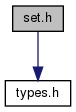
\includegraphics[width=129pt]{set_8h__incl}
\end{center}
\end{figure}
This graph shows which files directly or indirectly include this file\+:\nopagebreak
\begin{figure}[H]
\begin{center}
\leavevmode
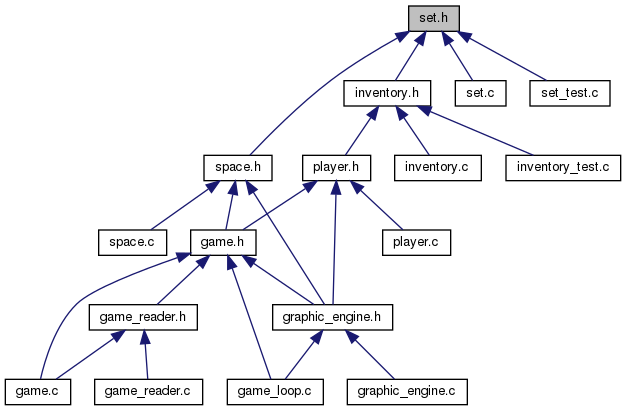
\includegraphics[width=350pt]{set_8h__dep__incl}
\end{center}
\end{figure}
\subsection*{Macros}
\begin{DoxyCompactItemize}
\item 
\#define \hyperlink{set_8h_a24b51e1a036e3b382adcc8216239aafd}{T\+A\+M\+\_\+\+S\+ET}~32
\end{DoxyCompactItemize}
\subsection*{Typedefs}
\begin{DoxyCompactItemize}
\item 
typedef struct \hyperlink{struct__Set}{\+\_\+\+Set} \hyperlink{set_8h_a6d3b7f7c92cbb4577ef3ef7ddbf93161}{Set}
\end{DoxyCompactItemize}
\subsection*{Functions}
\begin{DoxyCompactItemize}
\item 
\hyperlink{set_8h_a6d3b7f7c92cbb4577ef3ef7ddbf93161}{Set} $\ast$ \hyperlink{set_8h_abcc73b7ad3913fc92dd95d366c9c8687}{set\+\_\+create} ()
\begin{DoxyCompactList}\small\item\em crea un Set \end{DoxyCompactList}\item 
void \hyperlink{set_8h_a9d762a027f1c3bcdd22f70ee9093a7dd}{set\+\_\+destroy} (\hyperlink{set_8h_a6d3b7f7c92cbb4577ef3ef7ddbf93161}{Set} $\ast$set)
\begin{DoxyCompactList}\small\item\em destruye y libera la memoria de un Set \end{DoxyCompactList}\item 
\hyperlink{types_8h_a32c27cc471df37f4fc818d65de0a56c4}{S\+T\+A\+T\+US} \hyperlink{set_8h_a214235069ee276ad9bceb2c66e56bfe1}{set\+\_\+add} (\hyperlink{set_8h_a6d3b7f7c92cbb4577ef3ef7ddbf93161}{Set} $\ast$set, \hyperlink{types_8h_a845e604fb28f7e3d97549da3448149d3}{Id} id)
\begin{DoxyCompactList}\small\item\em añade un objeto a un Set \end{DoxyCompactList}\item 
\hyperlink{types_8h_a32c27cc471df37f4fc818d65de0a56c4}{S\+T\+A\+T\+US} \hyperlink{set_8h_a77f2edaabd819df68af4e1658cff9cfb}{set\+\_\+delete\+\_\+element} (\hyperlink{set_8h_a6d3b7f7c92cbb4577ef3ef7ddbf93161}{Set} $\ast$set, \hyperlink{types_8h_a845e604fb28f7e3d97549da3448149d3}{Id} id)
\begin{DoxyCompactList}\small\item\em borra un objeto de un Set \end{DoxyCompactList}\item 
int \hyperlink{set_8h_afaa9d55d67526584aba2e0688ca189b3}{set\+\_\+get\+\_\+num\+\_\+ids} (\hyperlink{set_8h_a6d3b7f7c92cbb4577ef3ef7ddbf93161}{Set} $\ast$set)
\begin{DoxyCompactList}\small\item\em devuelve el numero de objetos \end{DoxyCompactList}\item 
\hyperlink{types_8h_a3e5b8192e7d9ffaf3542f1210aec18dd}{B\+O\+OL} \hyperlink{set_8h_aac8585498aa55f445a6512bb8a2dfbf9}{set\+\_\+is\+\_\+id\+\_\+in} (\hyperlink{set_8h_a6d3b7f7c92cbb4577ef3ef7ddbf93161}{Set} $\ast$set, \hyperlink{types_8h_a845e604fb28f7e3d97549da3448149d3}{Id} id)
\begin{DoxyCompactList}\small\item\em comprueba si un objeto esta dentro de un set \end{DoxyCompactList}\item 
\hyperlink{types_8h_a3e5b8192e7d9ffaf3542f1210aec18dd}{B\+O\+OL} \hyperlink{set_8h_a57c0701d4c0160d762c7a233603020e7}{set\+\_\+is\+\_\+empty} (\hyperlink{set_8h_a6d3b7f7c92cbb4577ef3ef7ddbf93161}{Set} $\ast$set)
\begin{DoxyCompactList}\small\item\em comprueba si un set esta vacio \end{DoxyCompactList}\item 
\hyperlink{types_8h_a3e5b8192e7d9ffaf3542f1210aec18dd}{B\+O\+OL} \hyperlink{set_8h_aed6909525ac4a1e1dd0fee8afba53a37}{set\+\_\+is\+\_\+full} (\hyperlink{set_8h_a6d3b7f7c92cbb4577ef3ef7ddbf93161}{Set} $\ast$set)
\begin{DoxyCompactList}\small\item\em comprueba si un set esta lleno \end{DoxyCompactList}\item 
int \hyperlink{set_8h_acf28fd9289aabc528424ca9a865d5ed2}{set\+\_\+print} (F\+I\+LE $\ast$f, \hyperlink{set_8h_a6d3b7f7c92cbb4577ef3ef7ddbf93161}{Set} $\ast$set)
\begin{DoxyCompactList}\small\item\em imprime un set \end{DoxyCompactList}\end{DoxyCompactItemize}


\subsection{Detailed Description}
En este fichero implementamos las funciones de set. 

\begin{DoxyAuthor}{Author}
Manuel Suarez, Saul Almazán, Álvaro Becerra, Rodrigo Lardiés 
\end{DoxyAuthor}
\begin{DoxyVersion}{Version}
1.\+0 
\end{DoxyVersion}
\begin{DoxyDate}{Date}
20/10/2018 
\end{DoxyDate}


\subsection{Macro Definition Documentation}
\mbox{\Hypertarget{set_8h_a24b51e1a036e3b382adcc8216239aafd}\label{set_8h_a24b51e1a036e3b382adcc8216239aafd}} 
\index{set.\+h@{set.\+h}!T\+A\+M\+\_\+\+S\+ET@{T\+A\+M\+\_\+\+S\+ET}}
\index{T\+A\+M\+\_\+\+S\+ET@{T\+A\+M\+\_\+\+S\+ET}!set.\+h@{set.\+h}}
\subsubsection{\texorpdfstring{T\+A\+M\+\_\+\+S\+ET}{TAM\_SET}}
{\footnotesize\ttfamily \#define T\+A\+M\+\_\+\+S\+ET~32}

tamaño maximo del set 

\subsection{Typedef Documentation}
\mbox{\Hypertarget{set_8h_a6d3b7f7c92cbb4577ef3ef7ddbf93161}\label{set_8h_a6d3b7f7c92cbb4577ef3ef7ddbf93161}} 
\index{set.\+h@{set.\+h}!Set@{Set}}
\index{Set@{Set}!set.\+h@{set.\+h}}
\subsubsection{\texorpdfstring{Set}{Set}}
{\footnotesize\ttfamily typedef struct \hyperlink{struct__Set}{\+\_\+\+Set} \hyperlink{set_8h_a6d3b7f7c92cbb4577ef3ef7ddbf93161}{Set}}

Estructura de Set 

\subsection{Function Documentation}
\mbox{\Hypertarget{set_8h_a214235069ee276ad9bceb2c66e56bfe1}\label{set_8h_a214235069ee276ad9bceb2c66e56bfe1}} 
\index{set.\+h@{set.\+h}!set\+\_\+add@{set\+\_\+add}}
\index{set\+\_\+add@{set\+\_\+add}!set.\+h@{set.\+h}}
\subsubsection{\texorpdfstring{set\+\_\+add()}{set\_add()}}
{\footnotesize\ttfamily \hyperlink{types_8h_a32c27cc471df37f4fc818d65de0a56c4}{S\+T\+A\+T\+US} set\+\_\+add (\begin{DoxyParamCaption}\item[{\hyperlink{set_8h_a6d3b7f7c92cbb4577ef3ef7ddbf93161}{Set} $\ast$}]{set,  }\item[{\hyperlink{types_8h_a845e604fb28f7e3d97549da3448149d3}{Id}}]{id }\end{DoxyParamCaption})}



añade un objeto a un Set 

\begin{DoxyAuthor}{Author}
Manuel Suarez, Saul Almazán, Álvaro Becerra, Rodrigo Lardiés 
\end{DoxyAuthor}
\begin{DoxyDate}{Date}
20/10/2018 
\end{DoxyDate}

\begin{DoxyParams}{Parameters}
{\em set} & (El set a usar) \\
\hline
{\em id} & (El id del objeto que se añade al set) \\
\hline
\end{DoxyParams}
\begin{DoxyReturn}{Returns}
S\+T\+A\+T\+US (OK si se realiza con exito o E\+R\+R\+OR de lo contrario) 
\end{DoxyReturn}
\mbox{\Hypertarget{set_8h_abcc73b7ad3913fc92dd95d366c9c8687}\label{set_8h_abcc73b7ad3913fc92dd95d366c9c8687}} 
\index{set.\+h@{set.\+h}!set\+\_\+create@{set\+\_\+create}}
\index{set\+\_\+create@{set\+\_\+create}!set.\+h@{set.\+h}}
\subsubsection{\texorpdfstring{set\+\_\+create()}{set\_create()}}
{\footnotesize\ttfamily \hyperlink{set_8h_a6d3b7f7c92cbb4577ef3ef7ddbf93161}{Set}$\ast$ set\+\_\+create (\begin{DoxyParamCaption}{ }\end{DoxyParamCaption})}



crea un Set 

\begin{DoxyAuthor}{Author}
Manuel Suarez, Saul Almazán, Álvaro Becerra, Rodrigo Lardiés 
\end{DoxyAuthor}
\begin{DoxyDate}{Date}
20/10/2018 
\end{DoxyDate}
\begin{DoxyReturn}{Returns}
Set (El set que crea) 
\end{DoxyReturn}
\mbox{\Hypertarget{set_8h_a77f2edaabd819df68af4e1658cff9cfb}\label{set_8h_a77f2edaabd819df68af4e1658cff9cfb}} 
\index{set.\+h@{set.\+h}!set\+\_\+delete\+\_\+element@{set\+\_\+delete\+\_\+element}}
\index{set\+\_\+delete\+\_\+element@{set\+\_\+delete\+\_\+element}!set.\+h@{set.\+h}}
\subsubsection{\texorpdfstring{set\+\_\+delete\+\_\+element()}{set\_delete\_element()}}
{\footnotesize\ttfamily \hyperlink{types_8h_a32c27cc471df37f4fc818d65de0a56c4}{S\+T\+A\+T\+US} set\+\_\+delete\+\_\+element (\begin{DoxyParamCaption}\item[{\hyperlink{set_8h_a6d3b7f7c92cbb4577ef3ef7ddbf93161}{Set} $\ast$}]{set,  }\item[{\hyperlink{types_8h_a845e604fb28f7e3d97549da3448149d3}{Id}}]{id }\end{DoxyParamCaption})}



borra un objeto de un Set 

\begin{DoxyAuthor}{Author}
Manuel Suarez, Saul Almazán, Álvaro Becerra, Rodrigo Lardiés 
\end{DoxyAuthor}
\begin{DoxyDate}{Date}
20/10/2018 
\end{DoxyDate}

\begin{DoxyParams}{Parameters}
{\em set} & (El set a usar) \\
\hline
{\em id} & (El id del objeto que se borra del set) \\
\hline
\end{DoxyParams}
\begin{DoxyReturn}{Returns}
S\+T\+A\+T\+US (OK si se realiza con exito o E\+R\+R\+OR de lo contrario) 
\end{DoxyReturn}
\mbox{\Hypertarget{set_8h_a9d762a027f1c3bcdd22f70ee9093a7dd}\label{set_8h_a9d762a027f1c3bcdd22f70ee9093a7dd}} 
\index{set.\+h@{set.\+h}!set\+\_\+destroy@{set\+\_\+destroy}}
\index{set\+\_\+destroy@{set\+\_\+destroy}!set.\+h@{set.\+h}}
\subsubsection{\texorpdfstring{set\+\_\+destroy()}{set\_destroy()}}
{\footnotesize\ttfamily void set\+\_\+destroy (\begin{DoxyParamCaption}\item[{\hyperlink{set_8h_a6d3b7f7c92cbb4577ef3ef7ddbf93161}{Set} $\ast$}]{set }\end{DoxyParamCaption})}



destruye y libera la memoria de un Set 

\begin{DoxyAuthor}{Author}
Manuel Suarez, Saul Almazán, Álvaro Becerra, Rodrigo Lardiés 
\end{DoxyAuthor}
\begin{DoxyDate}{Date}
20/10/2018 
\end{DoxyDate}

\begin{DoxyParams}{Parameters}
{\em set} & (El set a destruir) \\
\hline
\end{DoxyParams}
\begin{DoxyReturn}{Returns}
void (No devuelve nada) 
\end{DoxyReturn}
\mbox{\Hypertarget{set_8h_afaa9d55d67526584aba2e0688ca189b3}\label{set_8h_afaa9d55d67526584aba2e0688ca189b3}} 
\index{set.\+h@{set.\+h}!set\+\_\+get\+\_\+num\+\_\+ids@{set\+\_\+get\+\_\+num\+\_\+ids}}
\index{set\+\_\+get\+\_\+num\+\_\+ids@{set\+\_\+get\+\_\+num\+\_\+ids}!set.\+h@{set.\+h}}
\subsubsection{\texorpdfstring{set\+\_\+get\+\_\+num\+\_\+ids()}{set\_get\_num\_ids()}}
{\footnotesize\ttfamily int set\+\_\+get\+\_\+num\+\_\+ids (\begin{DoxyParamCaption}\item[{\hyperlink{set_8h_a6d3b7f7c92cbb4577ef3ef7ddbf93161}{Set} $\ast$}]{set }\end{DoxyParamCaption})}



devuelve el numero de objetos 

\begin{DoxyAuthor}{Author}
Manuel Suarez, Saul Almazán, Álvaro Becerra, Rodrigo Lardiés 
\end{DoxyAuthor}
\begin{DoxyDate}{Date}
20/10/2018 
\end{DoxyDate}

\begin{DoxyParams}{Parameters}
{\em set} & (El set a usar) \\
\hline
\end{DoxyParams}
\begin{DoxyReturn}{Returns}
int (el numero de objetos) 
\end{DoxyReturn}
\mbox{\Hypertarget{set_8h_a57c0701d4c0160d762c7a233603020e7}\label{set_8h_a57c0701d4c0160d762c7a233603020e7}} 
\index{set.\+h@{set.\+h}!set\+\_\+is\+\_\+empty@{set\+\_\+is\+\_\+empty}}
\index{set\+\_\+is\+\_\+empty@{set\+\_\+is\+\_\+empty}!set.\+h@{set.\+h}}
\subsubsection{\texorpdfstring{set\+\_\+is\+\_\+empty()}{set\_is\_empty()}}
{\footnotesize\ttfamily \hyperlink{types_8h_a3e5b8192e7d9ffaf3542f1210aec18dd}{B\+O\+OL} set\+\_\+is\+\_\+empty (\begin{DoxyParamCaption}\item[{\hyperlink{set_8h_a6d3b7f7c92cbb4577ef3ef7ddbf93161}{Set} $\ast$}]{set }\end{DoxyParamCaption})}



comprueba si un set esta vacio 

\begin{DoxyAuthor}{Author}
Manuel Suarez, Saul Almazán, Álvaro Becerra, Rodrigo Lardiés 
\end{DoxyAuthor}
\begin{DoxyDate}{Date}
20/10/2018 
\end{DoxyDate}

\begin{DoxyParams}{Parameters}
{\em set} & (El set a usar) \\
\hline
\end{DoxyParams}
\begin{DoxyReturn}{Returns}
B\+O\+Ol (T\+R\+UE si el set esta vacio o F\+A\+L\+SE de lo contrario) 
\end{DoxyReturn}
\mbox{\Hypertarget{set_8h_aed6909525ac4a1e1dd0fee8afba53a37}\label{set_8h_aed6909525ac4a1e1dd0fee8afba53a37}} 
\index{set.\+h@{set.\+h}!set\+\_\+is\+\_\+full@{set\+\_\+is\+\_\+full}}
\index{set\+\_\+is\+\_\+full@{set\+\_\+is\+\_\+full}!set.\+h@{set.\+h}}
\subsubsection{\texorpdfstring{set\+\_\+is\+\_\+full()}{set\_is\_full()}}
{\footnotesize\ttfamily \hyperlink{types_8h_a3e5b8192e7d9ffaf3542f1210aec18dd}{B\+O\+OL} set\+\_\+is\+\_\+full (\begin{DoxyParamCaption}\item[{\hyperlink{set_8h_a6d3b7f7c92cbb4577ef3ef7ddbf93161}{Set} $\ast$}]{set }\end{DoxyParamCaption})}



comprueba si un set esta lleno 

\begin{DoxyAuthor}{Author}
Manuel Suarez, Saul Almazán, Álvaro Becerra, Rodrigo Lardiés 
\end{DoxyAuthor}
\begin{DoxyDate}{Date}
20/10/2018 
\end{DoxyDate}

\begin{DoxyParams}{Parameters}
{\em set} & (El set a usar) \\
\hline
\end{DoxyParams}
\begin{DoxyReturn}{Returns}
B\+O\+Ol (T\+R\+UE si el set esta lleno o F\+A\+L\+SE de lo contrario) 
\end{DoxyReturn}
\mbox{\Hypertarget{set_8h_aac8585498aa55f445a6512bb8a2dfbf9}\label{set_8h_aac8585498aa55f445a6512bb8a2dfbf9}} 
\index{set.\+h@{set.\+h}!set\+\_\+is\+\_\+id\+\_\+in@{set\+\_\+is\+\_\+id\+\_\+in}}
\index{set\+\_\+is\+\_\+id\+\_\+in@{set\+\_\+is\+\_\+id\+\_\+in}!set.\+h@{set.\+h}}
\subsubsection{\texorpdfstring{set\+\_\+is\+\_\+id\+\_\+in()}{set\_is\_id\_in()}}
{\footnotesize\ttfamily \hyperlink{types_8h_a3e5b8192e7d9ffaf3542f1210aec18dd}{B\+O\+OL} set\+\_\+is\+\_\+id\+\_\+in (\begin{DoxyParamCaption}\item[{\hyperlink{set_8h_a6d3b7f7c92cbb4577ef3ef7ddbf93161}{Set} $\ast$}]{set,  }\item[{\hyperlink{types_8h_a845e604fb28f7e3d97549da3448149d3}{Id}}]{id }\end{DoxyParamCaption})}



comprueba si un objeto esta dentro de un set 

\begin{DoxyAuthor}{Author}
Manuel Suarez, Saul Almazán, Álvaro Becerra, Rodrigo Lardiés 
\end{DoxyAuthor}
\begin{DoxyDate}{Date}
20/10/2018 
\end{DoxyDate}

\begin{DoxyParams}{Parameters}
{\em set} & (El set a usar) \\
\hline
{\em id} & (El id del objeto que se comprueba) \\
\hline
\end{DoxyParams}
\begin{DoxyReturn}{Returns}
B\+O\+Ol (T\+R\+UE si el objeto esta dentro del set o F\+A\+L\+SE de lo contrario) 
\end{DoxyReturn}
\mbox{\Hypertarget{set_8h_acf28fd9289aabc528424ca9a865d5ed2}\label{set_8h_acf28fd9289aabc528424ca9a865d5ed2}} 
\index{set.\+h@{set.\+h}!set\+\_\+print@{set\+\_\+print}}
\index{set\+\_\+print@{set\+\_\+print}!set.\+h@{set.\+h}}
\subsubsection{\texorpdfstring{set\+\_\+print()}{set\_print()}}
{\footnotesize\ttfamily int set\+\_\+print (\begin{DoxyParamCaption}\item[{F\+I\+LE $\ast$}]{f,  }\item[{\hyperlink{set_8h_a6d3b7f7c92cbb4577ef3ef7ddbf93161}{Set} $\ast$}]{set }\end{DoxyParamCaption})}



imprime un set 

\begin{DoxyAuthor}{Author}
Manuel Suarez, Saul Almazán, Álvaro Becerra, Rodrigo Lardiés 
\end{DoxyAuthor}
\begin{DoxyDate}{Date}
20/10/2018 
\end{DoxyDate}

\begin{DoxyParams}{Parameters}
{\em f} & (donde se va a imprimir) \\
\hline
{\em set} & (El set a imprimir) \\
\hline
\end{DoxyParams}
\begin{DoxyReturn}{Returns}
int (-\/1 si hay algun error) 
\end{DoxyReturn}

\hypertarget{set__test_8h}{}\section{include/set\+\_\+test.h File Reference}
\label{set__test_8h}\index{include/set\+\_\+test.\+h@{include/set\+\_\+test.\+h}}


Prueba del modulo player.  


This graph shows which files directly or indirectly include this file\+:
% FIG 0
\subsection*{Functions}
\begin{DoxyCompactItemize}
\item 
void \hyperlink{set__test_8h_a6f654ab4b44e8a9b9cedfb78c378a5d7}{test1\+\_\+set\+\_\+create} ()
\item 
void \hyperlink{set__test_8h_a4bec0c0f80b12fc9cabf5ed5ac6d1235}{test1\+\_\+set\+\_\+delete\+\_\+element} ()
\item 
void \hyperlink{set__test_8h_ac96b1e7b6602e3e491422053a43f08f6}{test2\+\_\+set\+\_\+delete\+\_\+element} ()
\item 
void \hyperlink{set__test_8h_a45af0aa2cb643d2809513f320a4f9af3}{test3\+\_\+set\+\_\+delete\+\_\+element} ()
\item 
void \hyperlink{set__test_8h_a014ebe1b46af5ea318143fc61894d9c0}{test1\+\_\+set\+\_\+add} ()
\item 
void \hyperlink{set__test_8h_ab09827322a313bf97b9757c98c2bdbb0}{test2\+\_\+set\+\_\+add} ()
\item 
void \hyperlink{set__test_8h_a7bae6941906dd98c8d8ffb2da8a409f6}{test1\+\_\+set\+\_\+is\+\_\+full} ()
\item 
void \hyperlink{set__test_8h_ab1de430f3e313725897f9b0b1aba543b}{test2\+\_\+set\+\_\+is\+\_\+full} ()
\item 
void \hyperlink{set__test_8h_a0d1505a528700bc71c89a71c88d6b21e}{test1\+\_\+set\+\_\+is\+\_\+empty} ()
\item 
void \hyperlink{set__test_8h_a13000e62535d3341e070963f4f3907ec}{test2\+\_\+set\+\_\+is\+\_\+empty} ()
\item 
void \hyperlink{set__test_8h_a44730a3c8aea8b09c4807d5a11794069}{test1\+\_\+set\+\_\+is\+\_\+id\+\_\+in} ()
\item 
void \hyperlink{set__test_8h_af068866754cc693dee41ee757c5ee4a2}{test2\+\_\+set\+\_\+is\+\_\+id\+\_\+in} ()
\item 
void \hyperlink{set__test_8h_a9a82ad51eca0f4cd5faf028e23b68bb3}{test1\+\_\+set\+\_\+get\+\_\+num\+\_\+ids} ()
\item 
void \hyperlink{set__test_8h_aaadf761f34e98a3a6d214cc2598ee852}{test2\+\_\+set\+\_\+get\+\_\+num\+\_\+ids} ()
\end{DoxyCompactItemize}


\subsection{Detailed Description}
Prueba del modulo player. 

\begin{DoxyAuthor}{Author}
Manuel Suarez, Saul Almazán, �?lvaro Becerra, Rodrigo Lardiés 
\end{DoxyAuthor}
\begin{DoxyVersion}{Version}
1.\+0 
\end{DoxyVersion}
\begin{DoxyDate}{Date}
12-\/11-\/2018 
\end{DoxyDate}


\subsection{Function Documentation}
\mbox{\Hypertarget{set__test_8h_a014ebe1b46af5ea318143fc61894d9c0}\label{set__test_8h_a014ebe1b46af5ea318143fc61894d9c0}} 
\index{set\+\_\+test.\+h@{set\+\_\+test.\+h}!test1\+\_\+set\+\_\+add@{test1\+\_\+set\+\_\+add}}
\index{test1\+\_\+set\+\_\+add@{test1\+\_\+set\+\_\+add}!set\+\_\+test.\+h@{set\+\_\+test.\+h}}
\subsubsection{\texorpdfstring{test1\+\_\+set\+\_\+add()}{test1\_set\_add()}}
{\footnotesize\ttfamily void test1\+\_\+set\+\_\+add (\begin{DoxyParamCaption}{ }\end{DoxyParamCaption})}

\begin{DoxyRefDesc}{Test}
\item[\hyperlink{test__test000231}{Test}]Prueba la función para añadir un objeto a un set \end{DoxyRefDesc}
\begin{DoxyPrecond}{Precondition}
id que establecer en el set 
\end{DoxyPrecond}
\begin{DoxyPostcond}{Postcondition}
La salida debe ser OK
\end{DoxyPostcond}
\begin{DoxyRefDesc}{Test}
\item[\hyperlink{test__test000111}{Test}]Prueba la función para añadir un objeto a un set \end{DoxyRefDesc}
\begin{DoxyPrecond}{Precondition}
id que establecer en el set 
\end{DoxyPrecond}
\begin{DoxyPostcond}{Postcondition}
La salida debe ser OK 
\end{DoxyPostcond}
\mbox{\Hypertarget{set__test_8h_a6f654ab4b44e8a9b9cedfb78c378a5d7}\label{set__test_8h_a6f654ab4b44e8a9b9cedfb78c378a5d7}} 
\index{set\+\_\+test.\+h@{set\+\_\+test.\+h}!test1\+\_\+set\+\_\+create@{test1\+\_\+set\+\_\+create}}
\index{test1\+\_\+set\+\_\+create@{test1\+\_\+set\+\_\+create}!set\+\_\+test.\+h@{set\+\_\+test.\+h}}
\subsubsection{\texorpdfstring{test1\+\_\+set\+\_\+create()}{test1\_set\_create()}}
{\footnotesize\ttfamily void test1\+\_\+set\+\_\+create (\begin{DoxyParamCaption}{ }\end{DoxyParamCaption})}

\begin{DoxyRefDesc}{Test}
\item[\hyperlink{test__test000227}{Test}]Prueba la función de creación de un set \end{DoxyRefDesc}
\begin{DoxyPrecond}{Precondition}
nada 
\end{DoxyPrecond}
\begin{DoxyPostcond}{Postcondition}
Un puntero no nulo al set creado
\end{DoxyPostcond}
\begin{DoxyRefDesc}{Test}
\item[\hyperlink{test__test000107}{Test}]Prueba la función de creación de un set \end{DoxyRefDesc}
\begin{DoxyPrecond}{Precondition}
nada 
\end{DoxyPrecond}
\begin{DoxyPostcond}{Postcondition}
Un puntero no nulo al set creado 
\end{DoxyPostcond}
\mbox{\Hypertarget{set__test_8h_a4bec0c0f80b12fc9cabf5ed5ac6d1235}\label{set__test_8h_a4bec0c0f80b12fc9cabf5ed5ac6d1235}} 
\index{set\+\_\+test.\+h@{set\+\_\+test.\+h}!test1\+\_\+set\+\_\+delete\+\_\+element@{test1\+\_\+set\+\_\+delete\+\_\+element}}
\index{test1\+\_\+set\+\_\+delete\+\_\+element@{test1\+\_\+set\+\_\+delete\+\_\+element}!set\+\_\+test.\+h@{set\+\_\+test.\+h}}
\subsubsection{\texorpdfstring{test1\+\_\+set\+\_\+delete\+\_\+element()}{test1\_set\_delete\_element()}}
{\footnotesize\ttfamily void test1\+\_\+set\+\_\+delete\+\_\+element (\begin{DoxyParamCaption}{ }\end{DoxyParamCaption})}

\begin{DoxyRefDesc}{Test}
\item[\hyperlink{test__test000228}{Test}]Prueba la función para borrar un objeto de un set \end{DoxyRefDesc}
\begin{DoxyPrecond}{Precondition}
set con un objeto 
\end{DoxyPrecond}
\begin{DoxyPostcond}{Postcondition}
La salida debe ser OK
\end{DoxyPostcond}
\begin{DoxyRefDesc}{Test}
\item[\hyperlink{test__test000108}{Test}]Prueba la función para borrar un objeto de un set \end{DoxyRefDesc}
\begin{DoxyPrecond}{Precondition}
set con un objeto 
\end{DoxyPrecond}
\begin{DoxyPostcond}{Postcondition}
La salida debe ser OK 
\end{DoxyPostcond}
\mbox{\Hypertarget{set__test_8h_a9a82ad51eca0f4cd5faf028e23b68bb3}\label{set__test_8h_a9a82ad51eca0f4cd5faf028e23b68bb3}} 
\index{set\+\_\+test.\+h@{set\+\_\+test.\+h}!test1\+\_\+set\+\_\+get\+\_\+num\+\_\+ids@{test1\+\_\+set\+\_\+get\+\_\+num\+\_\+ids}}
\index{test1\+\_\+set\+\_\+get\+\_\+num\+\_\+ids@{test1\+\_\+set\+\_\+get\+\_\+num\+\_\+ids}!set\+\_\+test.\+h@{set\+\_\+test.\+h}}
\subsubsection{\texorpdfstring{test1\+\_\+set\+\_\+get\+\_\+num\+\_\+ids()}{test1\_set\_get\_num\_ids()}}
{\footnotesize\ttfamily void test1\+\_\+set\+\_\+get\+\_\+num\+\_\+ids (\begin{DoxyParamCaption}{ }\end{DoxyParamCaption})}

\begin{DoxyRefDesc}{Test}
\item[\hyperlink{test__test000239}{Test}]Prueba la función para obtener el numero de ids de un set \end{DoxyRefDesc}
\begin{DoxyPrecond}{Precondition}
El set tiene cero ids 
\end{DoxyPrecond}
\begin{DoxyPostcond}{Postcondition}
La salida debe ser tam=0
\end{DoxyPostcond}
\begin{DoxyRefDesc}{Test}
\item[\hyperlink{test__test000119}{Test}]Prueba la función para obtener el numero de ids de un set \end{DoxyRefDesc}
\begin{DoxyPrecond}{Precondition}
El set tiene cero ids 
\end{DoxyPrecond}
\begin{DoxyPostcond}{Postcondition}
La salida debe ser tam=0 
\end{DoxyPostcond}
\mbox{\Hypertarget{set__test_8h_a0d1505a528700bc71c89a71c88d6b21e}\label{set__test_8h_a0d1505a528700bc71c89a71c88d6b21e}} 
\index{set\+\_\+test.\+h@{set\+\_\+test.\+h}!test1\+\_\+set\+\_\+is\+\_\+empty@{test1\+\_\+set\+\_\+is\+\_\+empty}}
\index{test1\+\_\+set\+\_\+is\+\_\+empty@{test1\+\_\+set\+\_\+is\+\_\+empty}!set\+\_\+test.\+h@{set\+\_\+test.\+h}}
\subsubsection{\texorpdfstring{test1\+\_\+set\+\_\+is\+\_\+empty()}{test1\_set\_is\_empty()}}
{\footnotesize\ttfamily void test1\+\_\+set\+\_\+is\+\_\+empty (\begin{DoxyParamCaption}{ }\end{DoxyParamCaption})}

\begin{DoxyRefDesc}{Test}
\item[\hyperlink{test__test000235}{Test}]Prueba la función para comprobar si un invetario está vacío \end{DoxyRefDesc}
\begin{DoxyPrecond}{Precondition}
set vacío 
\end{DoxyPrecond}
\begin{DoxyPostcond}{Postcondition}
La salida debe ser T\+R\+UE
\end{DoxyPostcond}
\begin{DoxyRefDesc}{Test}
\item[\hyperlink{test__test000115}{Test}]Prueba la función para comprobar si un invetario está vacío \end{DoxyRefDesc}
\begin{DoxyPrecond}{Precondition}
set vacío 
\end{DoxyPrecond}
\begin{DoxyPostcond}{Postcondition}
La salida debe ser T\+R\+UE 
\end{DoxyPostcond}
\mbox{\Hypertarget{set__test_8h_a7bae6941906dd98c8d8ffb2da8a409f6}\label{set__test_8h_a7bae6941906dd98c8d8ffb2da8a409f6}} 
\index{set\+\_\+test.\+h@{set\+\_\+test.\+h}!test1\+\_\+set\+\_\+is\+\_\+full@{test1\+\_\+set\+\_\+is\+\_\+full}}
\index{test1\+\_\+set\+\_\+is\+\_\+full@{test1\+\_\+set\+\_\+is\+\_\+full}!set\+\_\+test.\+h@{set\+\_\+test.\+h}}
\subsubsection{\texorpdfstring{test1\+\_\+set\+\_\+is\+\_\+full()}{test1\_set\_is\_full()}}
{\footnotesize\ttfamily void test1\+\_\+set\+\_\+is\+\_\+full (\begin{DoxyParamCaption}{ }\end{DoxyParamCaption})}

\begin{DoxyRefDesc}{Test}
\item[\hyperlink{test__test000233}{Test}]Prueba la función para comprobar si un invetario está lleno \end{DoxyRefDesc}
\begin{DoxyPrecond}{Precondition}
set vacío 
\end{DoxyPrecond}
\begin{DoxyPostcond}{Postcondition}
La salida debe ser F\+A\+L\+SE
\end{DoxyPostcond}
\begin{DoxyRefDesc}{Test}
\item[\hyperlink{test__test000113}{Test}]Prueba la función para comprobar si un invetario está lleno \end{DoxyRefDesc}
\begin{DoxyPrecond}{Precondition}
set vacío 
\end{DoxyPrecond}
\begin{DoxyPostcond}{Postcondition}
La salida debe ser F\+A\+L\+SE 
\end{DoxyPostcond}
\mbox{\Hypertarget{set__test_8h_a44730a3c8aea8b09c4807d5a11794069}\label{set__test_8h_a44730a3c8aea8b09c4807d5a11794069}} 
\index{set\+\_\+test.\+h@{set\+\_\+test.\+h}!test1\+\_\+set\+\_\+is\+\_\+id\+\_\+in@{test1\+\_\+set\+\_\+is\+\_\+id\+\_\+in}}
\index{test1\+\_\+set\+\_\+is\+\_\+id\+\_\+in@{test1\+\_\+set\+\_\+is\+\_\+id\+\_\+in}!set\+\_\+test.\+h@{set\+\_\+test.\+h}}
\subsubsection{\texorpdfstring{test1\+\_\+set\+\_\+is\+\_\+id\+\_\+in()}{test1\_set\_is\_id\_in()}}
{\footnotesize\ttfamily void test1\+\_\+set\+\_\+is\+\_\+id\+\_\+in (\begin{DoxyParamCaption}{ }\end{DoxyParamCaption})}

\begin{DoxyRefDesc}{Test}
\item[\hyperlink{test__test000237}{Test}]Prueba la función para saber si hay un objeto en el set \end{DoxyRefDesc}
\begin{DoxyPrecond}{Precondition}
El set tiene un objeto 
\end{DoxyPrecond}
\begin{DoxyPostcond}{Postcondition}
La salida debe ser T\+R\+UE
\end{DoxyPostcond}
\begin{DoxyRefDesc}{Test}
\item[\hyperlink{test__test000117}{Test}]Prueba la función para saber si hay un objeto en el set \end{DoxyRefDesc}
\begin{DoxyPrecond}{Precondition}
El set tiene un objeto 
\end{DoxyPrecond}
\begin{DoxyPostcond}{Postcondition}
La salida debe ser T\+R\+UE 
\end{DoxyPostcond}
\mbox{\Hypertarget{set__test_8h_ab09827322a313bf97b9757c98c2bdbb0}\label{set__test_8h_ab09827322a313bf97b9757c98c2bdbb0}} 
\index{set\+\_\+test.\+h@{set\+\_\+test.\+h}!test2\+\_\+set\+\_\+add@{test2\+\_\+set\+\_\+add}}
\index{test2\+\_\+set\+\_\+add@{test2\+\_\+set\+\_\+add}!set\+\_\+test.\+h@{set\+\_\+test.\+h}}
\subsubsection{\texorpdfstring{test2\+\_\+set\+\_\+add()}{test2\_set\_add()}}
{\footnotesize\ttfamily void test2\+\_\+set\+\_\+add (\begin{DoxyParamCaption}{ }\end{DoxyParamCaption})}

\begin{DoxyRefDesc}{Test}
\item[\hyperlink{test__test000232}{Test}]Prueba la función para añadir un objeto a un set \end{DoxyRefDesc}
\begin{DoxyPrecond}{Precondition}
id válido, pero set N\+U\+LL 
\end{DoxyPrecond}
\begin{DoxyPostcond}{Postcondition}
La salida debe ser E\+R\+R\+OR
\end{DoxyPostcond}
\begin{DoxyRefDesc}{Test}
\item[\hyperlink{test__test000112}{Test}]Prueba la función para añadir un objeto a un set \end{DoxyRefDesc}
\begin{DoxyPrecond}{Precondition}
id válido, pero set N\+U\+LL 
\end{DoxyPrecond}
\begin{DoxyPostcond}{Postcondition}
La salida debe ser E\+R\+R\+OR 
\end{DoxyPostcond}
\mbox{\Hypertarget{set__test_8h_ac96b1e7b6602e3e491422053a43f08f6}\label{set__test_8h_ac96b1e7b6602e3e491422053a43f08f6}} 
\index{set\+\_\+test.\+h@{set\+\_\+test.\+h}!test2\+\_\+set\+\_\+delete\+\_\+element@{test2\+\_\+set\+\_\+delete\+\_\+element}}
\index{test2\+\_\+set\+\_\+delete\+\_\+element@{test2\+\_\+set\+\_\+delete\+\_\+element}!set\+\_\+test.\+h@{set\+\_\+test.\+h}}
\subsubsection{\texorpdfstring{test2\+\_\+set\+\_\+delete\+\_\+element()}{test2\_set\_delete\_element()}}
{\footnotesize\ttfamily void test2\+\_\+set\+\_\+delete\+\_\+element (\begin{DoxyParamCaption}{ }\end{DoxyParamCaption})}

\begin{DoxyRefDesc}{Test}
\item[\hyperlink{test__test000229}{Test}]Prueba la función para borrar un objeto de un set \end{DoxyRefDesc}
\begin{DoxyPrecond}{Precondition}
set N\+U\+LL 
\end{DoxyPrecond}
\begin{DoxyPostcond}{Postcondition}
La salida debe ser E\+R\+R\+OR
\end{DoxyPostcond}
\begin{DoxyRefDesc}{Test}
\item[\hyperlink{test__test000109}{Test}]Prueba la función para borrar un objeto de un set \end{DoxyRefDesc}
\begin{DoxyPrecond}{Precondition}
set N\+U\+LL 
\end{DoxyPrecond}
\begin{DoxyPostcond}{Postcondition}
La salida debe ser E\+R\+R\+OR 
\end{DoxyPostcond}
\mbox{\Hypertarget{set__test_8h_aaadf761f34e98a3a6d214cc2598ee852}\label{set__test_8h_aaadf761f34e98a3a6d214cc2598ee852}} 
\index{set\+\_\+test.\+h@{set\+\_\+test.\+h}!test2\+\_\+set\+\_\+get\+\_\+num\+\_\+ids@{test2\+\_\+set\+\_\+get\+\_\+num\+\_\+ids}}
\index{test2\+\_\+set\+\_\+get\+\_\+num\+\_\+ids@{test2\+\_\+set\+\_\+get\+\_\+num\+\_\+ids}!set\+\_\+test.\+h@{set\+\_\+test.\+h}}
\subsubsection{\texorpdfstring{test2\+\_\+set\+\_\+get\+\_\+num\+\_\+ids()}{test2\_set\_get\_num\_ids()}}
{\footnotesize\ttfamily void test2\+\_\+set\+\_\+get\+\_\+num\+\_\+ids (\begin{DoxyParamCaption}{ }\end{DoxyParamCaption})}

\begin{DoxyRefDesc}{Test}
\item[\hyperlink{test__test000240}{Test}]Prueba la función para obtener el numero de ids de un set \end{DoxyRefDesc}
\begin{DoxyPrecond}{Precondition}
El set es N\+U\+LL 
\end{DoxyPrecond}
\begin{DoxyPostcond}{Postcondition}
La salida debe ser -\/1
\end{DoxyPostcond}
\begin{DoxyRefDesc}{Test}
\item[\hyperlink{test__test000120}{Test}]Prueba la función para obtener el numero de ids de un set \end{DoxyRefDesc}
\begin{DoxyPrecond}{Precondition}
El set es N\+U\+LL 
\end{DoxyPrecond}
\begin{DoxyPostcond}{Postcondition}
La salida debe ser -\/1 
\end{DoxyPostcond}
\mbox{\Hypertarget{set__test_8h_a13000e62535d3341e070963f4f3907ec}\label{set__test_8h_a13000e62535d3341e070963f4f3907ec}} 
\index{set\+\_\+test.\+h@{set\+\_\+test.\+h}!test2\+\_\+set\+\_\+is\+\_\+empty@{test2\+\_\+set\+\_\+is\+\_\+empty}}
\index{test2\+\_\+set\+\_\+is\+\_\+empty@{test2\+\_\+set\+\_\+is\+\_\+empty}!set\+\_\+test.\+h@{set\+\_\+test.\+h}}
\subsubsection{\texorpdfstring{test2\+\_\+set\+\_\+is\+\_\+empty()}{test2\_set\_is\_empty()}}
{\footnotesize\ttfamily void test2\+\_\+set\+\_\+is\+\_\+empty (\begin{DoxyParamCaption}{ }\end{DoxyParamCaption})}

\begin{DoxyRefDesc}{Test}
\item[\hyperlink{test__test000236}{Test}]Prueba la función para comprobar si un invetario está lleno \end{DoxyRefDesc}
\begin{DoxyPrecond}{Precondition}
set lleno 
\end{DoxyPrecond}
\begin{DoxyPostcond}{Postcondition}
La salida debe ser F\+A\+L\+SE
\end{DoxyPostcond}
\begin{DoxyRefDesc}{Test}
\item[\hyperlink{test__test000116}{Test}]Prueba la función para comprobar si un invetario está lleno \end{DoxyRefDesc}
\begin{DoxyPrecond}{Precondition}
set lleno 
\end{DoxyPrecond}
\begin{DoxyPostcond}{Postcondition}
La salida debe ser F\+A\+L\+SE 
\end{DoxyPostcond}
\mbox{\Hypertarget{set__test_8h_ab1de430f3e313725897f9b0b1aba543b}\label{set__test_8h_ab1de430f3e313725897f9b0b1aba543b}} 
\index{set\+\_\+test.\+h@{set\+\_\+test.\+h}!test2\+\_\+set\+\_\+is\+\_\+full@{test2\+\_\+set\+\_\+is\+\_\+full}}
\index{test2\+\_\+set\+\_\+is\+\_\+full@{test2\+\_\+set\+\_\+is\+\_\+full}!set\+\_\+test.\+h@{set\+\_\+test.\+h}}
\subsubsection{\texorpdfstring{test2\+\_\+set\+\_\+is\+\_\+full()}{test2\_set\_is\_full()}}
{\footnotesize\ttfamily void test2\+\_\+set\+\_\+is\+\_\+full (\begin{DoxyParamCaption}{ }\end{DoxyParamCaption})}

\begin{DoxyRefDesc}{Test}
\item[\hyperlink{test__test000234}{Test}]Prueba la función para comprobar si un invetario está lleno \end{DoxyRefDesc}
\begin{DoxyPrecond}{Precondition}
set lleno 
\end{DoxyPrecond}
\begin{DoxyPostcond}{Postcondition}
La salida debe ser T\+R\+UE
\end{DoxyPostcond}
\begin{DoxyRefDesc}{Test}
\item[\hyperlink{test__test000114}{Test}]Prueba la función para comprobar si un invetario está lleno \end{DoxyRefDesc}
\begin{DoxyPrecond}{Precondition}
set lleno 
\end{DoxyPrecond}
\begin{DoxyPostcond}{Postcondition}
La salida debe ser T\+R\+UE 
\end{DoxyPostcond}
\mbox{\Hypertarget{set__test_8h_af068866754cc693dee41ee757c5ee4a2}\label{set__test_8h_af068866754cc693dee41ee757c5ee4a2}} 
\index{set\+\_\+test.\+h@{set\+\_\+test.\+h}!test2\+\_\+set\+\_\+is\+\_\+id\+\_\+in@{test2\+\_\+set\+\_\+is\+\_\+id\+\_\+in}}
\index{test2\+\_\+set\+\_\+is\+\_\+id\+\_\+in@{test2\+\_\+set\+\_\+is\+\_\+id\+\_\+in}!set\+\_\+test.\+h@{set\+\_\+test.\+h}}
\subsubsection{\texorpdfstring{test2\+\_\+set\+\_\+is\+\_\+id\+\_\+in()}{test2\_set\_is\_id\_in()}}
{\footnotesize\ttfamily void test2\+\_\+set\+\_\+is\+\_\+id\+\_\+in (\begin{DoxyParamCaption}{ }\end{DoxyParamCaption})}

\begin{DoxyRefDesc}{Test}
\item[\hyperlink{test__test000238}{Test}]Prueba la función para saber si hay un objeto en el set \end{DoxyRefDesc}
\begin{DoxyPrecond}{Precondition}
El set es N\+U\+LL 
\end{DoxyPrecond}
\begin{DoxyPostcond}{Postcondition}
La salida debe ser F\+A\+L\+SE
\end{DoxyPostcond}
\begin{DoxyRefDesc}{Test}
\item[\hyperlink{test__test000118}{Test}]Prueba la función para saber si hay un objeto en el set \end{DoxyRefDesc}
\begin{DoxyPrecond}{Precondition}
El set es N\+U\+LL 
\end{DoxyPrecond}
\begin{DoxyPostcond}{Postcondition}
La salida debe ser F\+A\+L\+SE 
\end{DoxyPostcond}
\mbox{\Hypertarget{set__test_8h_a45af0aa2cb643d2809513f320a4f9af3}\label{set__test_8h_a45af0aa2cb643d2809513f320a4f9af3}} 
\index{set\+\_\+test.\+h@{set\+\_\+test.\+h}!test3\+\_\+set\+\_\+delete\+\_\+element@{test3\+\_\+set\+\_\+delete\+\_\+element}}
\index{test3\+\_\+set\+\_\+delete\+\_\+element@{test3\+\_\+set\+\_\+delete\+\_\+element}!set\+\_\+test.\+h@{set\+\_\+test.\+h}}
\subsubsection{\texorpdfstring{test3\+\_\+set\+\_\+delete\+\_\+element()}{test3\_set\_delete\_element()}}
{\footnotesize\ttfamily void test3\+\_\+set\+\_\+delete\+\_\+element (\begin{DoxyParamCaption}{ }\end{DoxyParamCaption})}

\begin{DoxyRefDesc}{Test}
\item[\hyperlink{test__test000230}{Test}]Prueba la función para borrar un objeto de un set \end{DoxyRefDesc}
\begin{DoxyPrecond}{Precondition}
set sin objetos 
\end{DoxyPrecond}
\begin{DoxyPostcond}{Postcondition}
La salida debe ser E\+R\+R\+OR
\end{DoxyPostcond}
\begin{DoxyRefDesc}{Test}
\item[\hyperlink{test__test000110}{Test}]Prueba la función para borrar un objeto de un set \end{DoxyRefDesc}
\begin{DoxyPrecond}{Precondition}
set sin objetos 
\end{DoxyPrecond}
\begin{DoxyPostcond}{Postcondition}
La salida debe ser E\+R\+R\+OR 
\end{DoxyPostcond}

\hypertarget{space_8h}{}\section{include/space.h File Reference}
\label{space_8h}\index{include/space.\+h@{include/space.\+h}}


En este fichero implementamos las funciones de space.  


{\ttfamily \#include \char`\"{}types.\+h\char`\"{}}\newline
{\ttfamily \#include \char`\"{}set.\+h\char`\"{}}\newline
Include dependency graph for space.\+h\+:
% FIG 0
This graph shows which files directly or indirectly include this file\+:
% FIG 1
\subsection*{Macros}
\begin{DoxyCompactItemize}
\item 
\#define \hyperlink{space_8h_a5f54fd55f983a2e33ce076cd9f587e82}{M\+A\+X\+\_\+\+S\+P\+A\+C\+ES}~10000
\item 
\#define \hyperlink{space_8h_a088cbe7c6f78264d46c2624194c5c680}{F\+I\+R\+S\+T\+\_\+\+S\+P\+A\+CE}~1
\item 
\#define \hyperlink{space_8h_a894ebc9b2098fe63607e0ca2e5f5ce8d}{T\+A\+M\+\_\+\+D\+I\+B\+U\+JO}~21
\item 
\#define \hyperlink{space_8h_ad29ae39d7c9da97f682d80fcee3e9fa4}{T\+A\+M\+\_\+\+D\+I\+B\+U\+J\+O\+\_\+\+L\+I\+N\+EA}~\hyperlink{space_8h_a894ebc9b2098fe63607e0ca2e5f5ce8d}{T\+A\+M\+\_\+\+D\+I\+B\+U\+JO}/3
\end{DoxyCompactItemize}
\subsection*{Typedefs}
\begin{DoxyCompactItemize}
\item 
typedef struct \hyperlink{struct__Space}{\+\_\+\+Space} \hyperlink{space_8h_a67533ffc2b70463baecc38fb0629bbfc}{Space}
\end{DoxyCompactItemize}
\subsection*{Functions}
\begin{DoxyCompactItemize}
\item 
\hyperlink{space_8h_a67533ffc2b70463baecc38fb0629bbfc}{Space} $\ast$ \hyperlink{space_8h_a162866fcea156b800fd546d0ffd271c9}{space\+\_\+create} (\hyperlink{types_8h_a845e604fb28f7e3d97549da3448149d3}{Id} id)
\begin{DoxyCompactList}\small\item\em crea un espacio \end{DoxyCompactList}\item 
\hyperlink{types_8h_a32c27cc471df37f4fc818d65de0a56c4}{S\+T\+A\+T\+US} \hyperlink{space_8h_a5c70c70398923693ddbe4dfac8d72a0d}{space\+\_\+destroy} (\hyperlink{space_8h_a67533ffc2b70463baecc38fb0629bbfc}{Space} $\ast$space)
\begin{DoxyCompactList}\small\item\em destruye y libera la memoria de un espacio \end{DoxyCompactList}\item 
\hyperlink{types_8h_a845e604fb28f7e3d97549da3448149d3}{Id} \hyperlink{space_8h_ac8ddfd0d8692fd852ee49698c446cb50}{space\+\_\+get\+\_\+id} (\hyperlink{space_8h_a67533ffc2b70463baecc38fb0629bbfc}{Space} $\ast$space)
\begin{DoxyCompactList}\small\item\em devuelve el Id del espacio \end{DoxyCompactList}\item 
\hyperlink{types_8h_a32c27cc471df37f4fc818d65de0a56c4}{S\+T\+A\+T\+US} \hyperlink{space_8h_aab5b468f9822ab78dbe16d1321870d93}{space\+\_\+set\+\_\+name} (\hyperlink{space_8h_a67533ffc2b70463baecc38fb0629bbfc}{Space} $\ast$space, char $\ast$name)
\begin{DoxyCompactList}\small\item\em cambia el nombre del espacio \end{DoxyCompactList}\item 
const char $\ast$ \hyperlink{space_8h_a310c540cd6e11073f7328add1f927001}{space\+\_\+get\+\_\+name} (\hyperlink{space_8h_a67533ffc2b70463baecc38fb0629bbfc}{Space} $\ast$space)
\begin{DoxyCompactList}\small\item\em devuelve el nombre del espacio \end{DoxyCompactList}\item 
\hyperlink{types_8h_a32c27cc471df37f4fc818d65de0a56c4}{S\+T\+A\+T\+US} \hyperlink{space_8h_a9e6e3e3bac4996ac6b8bd555e52bfb26}{space\+\_\+set\+\_\+north} (\hyperlink{space_8h_a67533ffc2b70463baecc38fb0629bbfc}{Space} $\ast$space, \hyperlink{types_8h_a845e604fb28f7e3d97549da3448149d3}{Id} id)
\begin{DoxyCompactList}\small\item\em cambia el Id del norte del espacio \end{DoxyCompactList}\item 
\hyperlink{types_8h_a845e604fb28f7e3d97549da3448149d3}{Id} \hyperlink{space_8h_ad331fba774897900f615d9d2e8d81a90}{space\+\_\+get\+\_\+north} (\hyperlink{space_8h_a67533ffc2b70463baecc38fb0629bbfc}{Space} $\ast$space)
\begin{DoxyCompactList}\small\item\em devuelve el Id del norte \end{DoxyCompactList}\item 
\hyperlink{types_8h_a32c27cc471df37f4fc818d65de0a56c4}{S\+T\+A\+T\+US} \hyperlink{space_8h_a422ab9f220b4c471c44256a27377de1a}{space\+\_\+set\+\_\+south} (\hyperlink{space_8h_a67533ffc2b70463baecc38fb0629bbfc}{Space} $\ast$space, \hyperlink{types_8h_a845e604fb28f7e3d97549da3448149d3}{Id} id)
\begin{DoxyCompactList}\small\item\em cambia el Id del sur del espacio \end{DoxyCompactList}\item 
\hyperlink{types_8h_a845e604fb28f7e3d97549da3448149d3}{Id} \hyperlink{space_8h_a9b86e1335c423eaad832e50d4c12cf1f}{space\+\_\+get\+\_\+south} (\hyperlink{space_8h_a67533ffc2b70463baecc38fb0629bbfc}{Space} $\ast$space)
\begin{DoxyCompactList}\small\item\em devuelve el Id del sur \end{DoxyCompactList}\item 
\hyperlink{types_8h_a32c27cc471df37f4fc818d65de0a56c4}{S\+T\+A\+T\+US} \hyperlink{space_8h_a860a8f3e0227955ad56d1a12f0bdc44a}{space\+\_\+set\+\_\+east} (\hyperlink{space_8h_a67533ffc2b70463baecc38fb0629bbfc}{Space} $\ast$space, \hyperlink{types_8h_a845e604fb28f7e3d97549da3448149d3}{Id} id)
\begin{DoxyCompactList}\small\item\em cambia el Id del este del espacio \end{DoxyCompactList}\item 
\hyperlink{types_8h_a845e604fb28f7e3d97549da3448149d3}{Id} \hyperlink{space_8h_a978a22b77f74bb2dab68a00571abbe0b}{space\+\_\+get\+\_\+east} (\hyperlink{space_8h_a67533ffc2b70463baecc38fb0629bbfc}{Space} $\ast$space)
\begin{DoxyCompactList}\small\item\em devuelve el Id del este \end{DoxyCompactList}\item 
\hyperlink{types_8h_a32c27cc471df37f4fc818d65de0a56c4}{S\+T\+A\+T\+US} \hyperlink{space_8h_ad44b14cb38902cf31fa1f341beaab0db}{space\+\_\+set\+\_\+west} (\hyperlink{space_8h_a67533ffc2b70463baecc38fb0629bbfc}{Space} $\ast$space, \hyperlink{types_8h_a845e604fb28f7e3d97549da3448149d3}{Id} id)
\begin{DoxyCompactList}\small\item\em cambia el Id del oeste del espacio \end{DoxyCompactList}\item 
\hyperlink{types_8h_a845e604fb28f7e3d97549da3448149d3}{Id} \hyperlink{space_8h_af495ebfd5d13eba1a48cebd10992a17f}{space\+\_\+get\+\_\+west} (\hyperlink{space_8h_a67533ffc2b70463baecc38fb0629bbfc}{Space} $\ast$space)
\begin{DoxyCompactList}\small\item\em devuelve el Id del oeste \end{DoxyCompactList}\item 
\hyperlink{types_8h_a3e5b8192e7d9ffaf3542f1210aec18dd}{B\+O\+OL} \hyperlink{space_8h_aac1e07503b3a4e740444c1318f6ea868}{space\+\_\+is\+\_\+object\+\_\+in} (\hyperlink{space_8h_a67533ffc2b70463baecc38fb0629bbfc}{Space} $\ast$space, \hyperlink{types_8h_a845e604fb28f7e3d97549da3448149d3}{Id} id)
\begin{DoxyCompactList}\small\item\em comprueba si hay un objeto en el espacio \end{DoxyCompactList}\item 
\hyperlink{types_8h_a32c27cc471df37f4fc818d65de0a56c4}{S\+T\+A\+T\+US} \hyperlink{space_8h_a18eca058da6cdf20ae5eda9d122d992e}{space\+\_\+print} (\hyperlink{space_8h_a67533ffc2b70463baecc38fb0629bbfc}{Space} $\ast$space)
\begin{DoxyCompactList}\small\item\em imprime el espacio \end{DoxyCompactList}\item 
\hyperlink{types_8h_a32c27cc471df37f4fc818d65de0a56c4}{S\+T\+A\+T\+US} \hyperlink{space_8h_af845878ae403cdd733520bb96e2385ea}{space\+\_\+take\+\_\+object} (\hyperlink{space_8h_a67533ffc2b70463baecc38fb0629bbfc}{Space} $\ast$space, \hyperlink{types_8h_a845e604fb28f7e3d97549da3448149d3}{Id} id)
\begin{DoxyCompactList}\small\item\em coge un objeto del espacio \end{DoxyCompactList}\item 
\hyperlink{types_8h_a32c27cc471df37f4fc818d65de0a56c4}{S\+T\+A\+T\+US} \hyperlink{space_8h_af038679271749a0298ba4a7c2efd46ed}{space\+\_\+leave\+\_\+object} (\hyperlink{space_8h_a67533ffc2b70463baecc38fb0629bbfc}{Space} $\ast$space, \hyperlink{types_8h_a845e604fb28f7e3d97549da3448149d3}{Id} id)
\begin{DoxyCompactList}\small\item\em suelta un objeto del espacio \end{DoxyCompactList}\item 
char $\ast$ \hyperlink{space_8h_a757f05fd67a488ddd96a541b7743520f}{space\+\_\+get\+\_\+gdesc} (\hyperlink{space_8h_a67533ffc2b70463baecc38fb0629bbfc}{Space} $\ast$)
\begin{DoxyCompactList}\small\item\em devuelve el contenido del espacio \end{DoxyCompactList}\item 
\hyperlink{types_8h_a32c27cc471df37f4fc818d65de0a56c4}{S\+T\+A\+T\+US} \hyperlink{space_8h_af71d1536b5452e698e670d61a4f0376f}{space\+\_\+set\+\_\+gdesc} (\hyperlink{space_8h_a67533ffc2b70463baecc38fb0629bbfc}{Space} $\ast$, char $\ast$)
\begin{DoxyCompactList}\small\item\em cambia el contenido del espacio \end{DoxyCompactList}\item 
char $\ast$ \hyperlink{space_8h_a292ba89734c883f99015a8b6ec147be8}{space\+\_\+get\+\_\+description} (\hyperlink{space_8h_a67533ffc2b70463baecc38fb0629bbfc}{Space} $\ast$space)
\begin{DoxyCompactList}\small\item\em devuelve la descripcion del espacio \end{DoxyCompactList}\item 
\hyperlink{types_8h_a32c27cc471df37f4fc818d65de0a56c4}{S\+T\+A\+T\+US} \hyperlink{space_8h_a7aecc426029f567d452a0f916fd512d6}{space\+\_\+set\+\_\+description} (\hyperlink{space_8h_a67533ffc2b70463baecc38fb0629bbfc}{Space} $\ast$space, char $\ast$description)
\begin{DoxyCompactList}\small\item\em cambia la descripcion del espacio \end{DoxyCompactList}\item 
\hyperlink{types_8h_a32c27cc471df37f4fc818d65de0a56c4}{S\+T\+A\+T\+US} \hyperlink{space_8h_a08ee81e588e2ce8744e0c9abc2b5f2c7}{space\+\_\+set\+\_\+detailed\+\_\+description} (\hyperlink{space_8h_a67533ffc2b70463baecc38fb0629bbfc}{Space} $\ast$space, char $\ast$description)
\begin{DoxyCompactList}\small\item\em cambia la descripcion detallada del espacio \end{DoxyCompactList}\item 
char $\ast$ \hyperlink{space_8h_a478db36871e852912a3ae266c58145dc}{space\+\_\+get\+\_\+detailed\+\_\+description} (\hyperlink{space_8h_a67533ffc2b70463baecc38fb0629bbfc}{Space} $\ast$space)
\begin{DoxyCompactList}\small\item\em devuelve la descripcion detallada del espacio \end{DoxyCompactList}\item 
\hyperlink{types_8h_a845e604fb28f7e3d97549da3448149d3}{Id} \hyperlink{space_8h_a174a988b899d5a0db889a31b70763c9c}{space\+\_\+get\+\_\+up} (\hyperlink{space_8h_a67533ffc2b70463baecc38fb0629bbfc}{Space} $\ast$space)
\begin{DoxyCompactList}\small\item\em devuelve el Id arriba \end{DoxyCompactList}\item 
\hyperlink{types_8h_a845e604fb28f7e3d97549da3448149d3}{Id} \hyperlink{space_8h_ab269eab72b9ea7254044b34b1c177602}{space\+\_\+get\+\_\+down} (\hyperlink{space_8h_a67533ffc2b70463baecc38fb0629bbfc}{Space} $\ast$space)
\begin{DoxyCompactList}\small\item\em devuelve el Id abajo \end{DoxyCompactList}\item 
\hyperlink{types_8h_a3e5b8192e7d9ffaf3542f1210aec18dd}{B\+O\+OL} \hyperlink{space_8h_abae16fa836379f9fa4b22d9417b317b0}{space\+\_\+get\+\_\+light} (\hyperlink{space_8h_a67533ffc2b70463baecc38fb0629bbfc}{Space} $\ast$space)
\begin{DoxyCompactList}\small\item\em devuelve el estado de iluminación \end{DoxyCompactList}\item 
\hyperlink{types_8h_a32c27cc471df37f4fc818d65de0a56c4}{S\+T\+A\+T\+US} \hyperlink{space_8h_aa2707bdca8fd356ed8d15fd48e820a4f}{space\+\_\+set\+\_\+up} (\hyperlink{space_8h_a67533ffc2b70463baecc38fb0629bbfc}{Space} $\ast$space, \hyperlink{types_8h_a845e604fb28f7e3d97549da3448149d3}{Id} id)
\begin{DoxyCompactList}\small\item\em cambia el Id de arriba del espacio \end{DoxyCompactList}\item 
\hyperlink{types_8h_a32c27cc471df37f4fc818d65de0a56c4}{S\+T\+A\+T\+US} \hyperlink{space_8h_ae5b9fef52456ffccffbd73f882a56d23}{space\+\_\+set\+\_\+down} (\hyperlink{space_8h_a67533ffc2b70463baecc38fb0629bbfc}{Space} $\ast$space, \hyperlink{types_8h_a845e604fb28f7e3d97549da3448149d3}{Id} id)
\begin{DoxyCompactList}\small\item\em cambia el Id de abajo del espacio \end{DoxyCompactList}\item 
\hyperlink{types_8h_a32c27cc471df37f4fc818d65de0a56c4}{S\+T\+A\+T\+US} \hyperlink{space_8h_ad6a4bfb3b69236212c618d4c86181608}{space\+\_\+set\+\_\+light} (\hyperlink{space_8h_a67533ffc2b70463baecc38fb0629bbfc}{Space} $\ast$space, \hyperlink{types_8h_a3e5b8192e7d9ffaf3542f1210aec18dd}{B\+O\+OL} status)
\begin{DoxyCompactList}\small\item\em cambia el estado de iluminación de un espacio \end{DoxyCompactList}\end{DoxyCompactItemize}


\subsection{Detailed Description}
En este fichero implementamos las funciones de space. 

\begin{DoxyAuthor}{Author}
Manuel Suarez, Saul Almazán, Álvaro Becerra, Rodrigo Lardiés 
\end{DoxyAuthor}
\begin{DoxyVersion}{Version}
1.\+0 
\end{DoxyVersion}
\begin{DoxyDate}{Date}
20/10/2018 
\end{DoxyDate}


\subsection{Macro Definition Documentation}
\mbox{\Hypertarget{space_8h_a088cbe7c6f78264d46c2624194c5c680}\label{space_8h_a088cbe7c6f78264d46c2624194c5c680}} 
\index{space.\+h@{space.\+h}!F\+I\+R\+S\+T\+\_\+\+S\+P\+A\+CE@{F\+I\+R\+S\+T\+\_\+\+S\+P\+A\+CE}}
\index{F\+I\+R\+S\+T\+\_\+\+S\+P\+A\+CE@{F\+I\+R\+S\+T\+\_\+\+S\+P\+A\+CE}!space.\+h@{space.\+h}}
\subsubsection{\texorpdfstring{F\+I\+R\+S\+T\+\_\+\+S\+P\+A\+CE}{FIRST\_SPACE}}
{\footnotesize\ttfamily \#define F\+I\+R\+S\+T\+\_\+\+S\+P\+A\+CE~1}

primer espacio \mbox{\Hypertarget{space_8h_a5f54fd55f983a2e33ce076cd9f587e82}\label{space_8h_a5f54fd55f983a2e33ce076cd9f587e82}} 
\index{space.\+h@{space.\+h}!M\+A\+X\+\_\+\+S\+P\+A\+C\+ES@{M\+A\+X\+\_\+\+S\+P\+A\+C\+ES}}
\index{M\+A\+X\+\_\+\+S\+P\+A\+C\+ES@{M\+A\+X\+\_\+\+S\+P\+A\+C\+ES}!space.\+h@{space.\+h}}
\subsubsection{\texorpdfstring{M\+A\+X\+\_\+\+S\+P\+A\+C\+ES}{MAX\_SPACES}}
{\footnotesize\ttfamily \#define M\+A\+X\+\_\+\+S\+P\+A\+C\+ES~10000}

maximo de espacios \mbox{\Hypertarget{space_8h_a894ebc9b2098fe63607e0ca2e5f5ce8d}\label{space_8h_a894ebc9b2098fe63607e0ca2e5f5ce8d}} 
\index{space.\+h@{space.\+h}!T\+A\+M\+\_\+\+D\+I\+B\+U\+JO@{T\+A\+M\+\_\+\+D\+I\+B\+U\+JO}}
\index{T\+A\+M\+\_\+\+D\+I\+B\+U\+JO@{T\+A\+M\+\_\+\+D\+I\+B\+U\+JO}!space.\+h@{space.\+h}}
\subsubsection{\texorpdfstring{T\+A\+M\+\_\+\+D\+I\+B\+U\+JO}{TAM\_DIBUJO}}
{\footnotesize\ttfamily \#define T\+A\+M\+\_\+\+D\+I\+B\+U\+JO~21}

maximo de dibujo \mbox{\Hypertarget{space_8h_ad29ae39d7c9da97f682d80fcee3e9fa4}\label{space_8h_ad29ae39d7c9da97f682d80fcee3e9fa4}} 
\index{space.\+h@{space.\+h}!T\+A\+M\+\_\+\+D\+I\+B\+U\+J\+O\+\_\+\+L\+I\+N\+EA@{T\+A\+M\+\_\+\+D\+I\+B\+U\+J\+O\+\_\+\+L\+I\+N\+EA}}
\index{T\+A\+M\+\_\+\+D\+I\+B\+U\+J\+O\+\_\+\+L\+I\+N\+EA@{T\+A\+M\+\_\+\+D\+I\+B\+U\+J\+O\+\_\+\+L\+I\+N\+EA}!space.\+h@{space.\+h}}
\subsubsection{\texorpdfstring{T\+A\+M\+\_\+\+D\+I\+B\+U\+J\+O\+\_\+\+L\+I\+N\+EA}{TAM\_DIBUJO\_LINEA}}
{\footnotesize\ttfamily \#define T\+A\+M\+\_\+\+D\+I\+B\+U\+J\+O\+\_\+\+L\+I\+N\+EA~\hyperlink{space_8h_a894ebc9b2098fe63607e0ca2e5f5ce8d}{T\+A\+M\+\_\+\+D\+I\+B\+U\+JO}/3}

maximo del dibujo de cada linea 

\subsection{Typedef Documentation}
\mbox{\Hypertarget{space_8h_a67533ffc2b70463baecc38fb0629bbfc}\label{space_8h_a67533ffc2b70463baecc38fb0629bbfc}} 
\index{space.\+h@{space.\+h}!Space@{Space}}
\index{Space@{Space}!space.\+h@{space.\+h}}
\subsubsection{\texorpdfstring{Space}{Space}}
{\footnotesize\ttfamily typedef struct \hyperlink{struct__Space}{\+\_\+\+Space} \hyperlink{space_8h_a67533ffc2b70463baecc38fb0629bbfc}{Space}}

Estructura de espacio 

\subsection{Function Documentation}
\mbox{\Hypertarget{space_8h_a162866fcea156b800fd546d0ffd271c9}\label{space_8h_a162866fcea156b800fd546d0ffd271c9}} 
\index{space.\+h@{space.\+h}!space\+\_\+create@{space\+\_\+create}}
\index{space\+\_\+create@{space\+\_\+create}!space.\+h@{space.\+h}}
\subsubsection{\texorpdfstring{space\+\_\+create()}{space\_create()}}
{\footnotesize\ttfamily \hyperlink{space_8h_a67533ffc2b70463baecc38fb0629bbfc}{Space}$\ast$ space\+\_\+create (\begin{DoxyParamCaption}\item[{\hyperlink{types_8h_a845e604fb28f7e3d97549da3448149d3}{Id}}]{id }\end{DoxyParamCaption})}



crea un espacio 

\begin{DoxyAuthor}{Author}
Manuel Suarez, Saul Almazán, Álvaro Becerra, Rodrigo Lardiés 
\end{DoxyAuthor}
\begin{DoxyDate}{Date}
10/11/2018 
\end{DoxyDate}

\begin{DoxyParams}{Parameters}
{\em id} & (id del nuevo espacio) \\
\hline
\end{DoxyParams}
\begin{DoxyReturn}{Returns}
Space$\ast$ (El espacio que crea) 
\end{DoxyReturn}
\mbox{\Hypertarget{space_8h_a5c70c70398923693ddbe4dfac8d72a0d}\label{space_8h_a5c70c70398923693ddbe4dfac8d72a0d}} 
\index{space.\+h@{space.\+h}!space\+\_\+destroy@{space\+\_\+destroy}}
\index{space\+\_\+destroy@{space\+\_\+destroy}!space.\+h@{space.\+h}}
\subsubsection{\texorpdfstring{space\+\_\+destroy()}{space\_destroy()}}
{\footnotesize\ttfamily \hyperlink{types_8h_a32c27cc471df37f4fc818d65de0a56c4}{S\+T\+A\+T\+US} space\+\_\+destroy (\begin{DoxyParamCaption}\item[{\hyperlink{space_8h_a67533ffc2b70463baecc38fb0629bbfc}{Space} $\ast$}]{space }\end{DoxyParamCaption})}



destruye y libera la memoria de un espacio 

\begin{DoxyAuthor}{Author}
Manuel Suarez, Saul Almazán, Álvaro Becerra, Rodrigo Lardiés 
\end{DoxyAuthor}
\begin{DoxyDate}{Date}
10/11/2018 
\end{DoxyDate}

\begin{DoxyParams}{Parameters}
{\em space} & (el espacio a destruir) \\
\hline
\end{DoxyParams}
\begin{DoxyReturn}{Returns}
S\+T\+A\+T\+US (Ok si se ha realizado con exito o E\+R\+R\+OR de lo contrario) 
\end{DoxyReturn}
\mbox{\Hypertarget{space_8h_a292ba89734c883f99015a8b6ec147be8}\label{space_8h_a292ba89734c883f99015a8b6ec147be8}} 
\index{space.\+h@{space.\+h}!space\+\_\+get\+\_\+description@{space\+\_\+get\+\_\+description}}
\index{space\+\_\+get\+\_\+description@{space\+\_\+get\+\_\+description}!space.\+h@{space.\+h}}
\subsubsection{\texorpdfstring{space\+\_\+get\+\_\+description()}{space\_get\_description()}}
{\footnotesize\ttfamily char$\ast$ space\+\_\+get\+\_\+description (\begin{DoxyParamCaption}\item[{\hyperlink{space_8h_a67533ffc2b70463baecc38fb0629bbfc}{Space} $\ast$}]{space }\end{DoxyParamCaption})}



devuelve la descripcion del espacio 

\begin{DoxyAuthor}{Author}
Manuel Suarez, Saul Almazán, Álvaro Becerra, Rodrigo Lardiés 
\end{DoxyAuthor}
\begin{DoxyDate}{Date}
10/11/2018 
\end{DoxyDate}

\begin{DoxyParams}{Parameters}
{\em space} & (espacio a usar) \\
\hline
\end{DoxyParams}
\begin{DoxyReturn}{Returns}
char (La descripcion del espacio) 
\end{DoxyReturn}
\mbox{\Hypertarget{space_8h_a478db36871e852912a3ae266c58145dc}\label{space_8h_a478db36871e852912a3ae266c58145dc}} 
\index{space.\+h@{space.\+h}!space\+\_\+get\+\_\+detailed\+\_\+description@{space\+\_\+get\+\_\+detailed\+\_\+description}}
\index{space\+\_\+get\+\_\+detailed\+\_\+description@{space\+\_\+get\+\_\+detailed\+\_\+description}!space.\+h@{space.\+h}}
\subsubsection{\texorpdfstring{space\+\_\+get\+\_\+detailed\+\_\+description()}{space\_get\_detailed\_description()}}
{\footnotesize\ttfamily char$\ast$ space\+\_\+get\+\_\+detailed\+\_\+description (\begin{DoxyParamCaption}\item[{\hyperlink{space_8h_a67533ffc2b70463baecc38fb0629bbfc}{Space} $\ast$}]{space }\end{DoxyParamCaption})}



devuelve la descripcion detallada del espacio 

\begin{DoxyAuthor}{Author}
Manuel Suarez, Saul Almazán, Álvaro Becerra, Rodrigo Lardiés 
\end{DoxyAuthor}
\begin{DoxyDate}{Date}
23/11/2018 
\end{DoxyDate}

\begin{DoxyParams}{Parameters}
{\em space} & (espacio a usar) \\
\hline
\end{DoxyParams}
\begin{DoxyReturn}{Returns}
char (La descripcion del espacio) 
\end{DoxyReturn}
\mbox{\Hypertarget{space_8h_ab269eab72b9ea7254044b34b1c177602}\label{space_8h_ab269eab72b9ea7254044b34b1c177602}} 
\index{space.\+h@{space.\+h}!space\+\_\+get\+\_\+down@{space\+\_\+get\+\_\+down}}
\index{space\+\_\+get\+\_\+down@{space\+\_\+get\+\_\+down}!space.\+h@{space.\+h}}
\subsubsection{\texorpdfstring{space\+\_\+get\+\_\+down()}{space\_get\_down()}}
{\footnotesize\ttfamily \hyperlink{types_8h_a845e604fb28f7e3d97549da3448149d3}{Id} space\+\_\+get\+\_\+down (\begin{DoxyParamCaption}\item[{\hyperlink{space_8h_a67533ffc2b70463baecc38fb0629bbfc}{Space} $\ast$}]{space }\end{DoxyParamCaption})}



devuelve el Id abajo 

\begin{DoxyAuthor}{Author}
Manuel Suarez, Saul Almazán, Álvaro Becerra, Rodrigo Lardiés 
\end{DoxyAuthor}
\begin{DoxyDate}{Date}
22/11/2018 
\end{DoxyDate}

\begin{DoxyParams}{Parameters}
{\em space} & (espacio a usar) \\
\hline
\end{DoxyParams}
\begin{DoxyReturn}{Returns}
Id(devuelve el Id abajo) 
\end{DoxyReturn}
\mbox{\Hypertarget{space_8h_a978a22b77f74bb2dab68a00571abbe0b}\label{space_8h_a978a22b77f74bb2dab68a00571abbe0b}} 
\index{space.\+h@{space.\+h}!space\+\_\+get\+\_\+east@{space\+\_\+get\+\_\+east}}
\index{space\+\_\+get\+\_\+east@{space\+\_\+get\+\_\+east}!space.\+h@{space.\+h}}
\subsubsection{\texorpdfstring{space\+\_\+get\+\_\+east()}{space\_get\_east()}}
{\footnotesize\ttfamily \hyperlink{types_8h_a845e604fb28f7e3d97549da3448149d3}{Id} space\+\_\+get\+\_\+east (\begin{DoxyParamCaption}\item[{\hyperlink{space_8h_a67533ffc2b70463baecc38fb0629bbfc}{Space} $\ast$}]{space }\end{DoxyParamCaption})}



devuelve el Id del este 

\begin{DoxyAuthor}{Author}
Manuel Suarez, Saul Almazán, Álvaro Becerra, Rodrigo Lardiés 
\end{DoxyAuthor}
\begin{DoxyDate}{Date}
10/11/2018 
\end{DoxyDate}

\begin{DoxyParams}{Parameters}
{\em space} & (espacio a usar) \\
\hline
\end{DoxyParams}
\begin{DoxyReturn}{Returns}
Id(devuelve el Id del este) 
\end{DoxyReturn}
\mbox{\Hypertarget{space_8h_a757f05fd67a488ddd96a541b7743520f}\label{space_8h_a757f05fd67a488ddd96a541b7743520f}} 
\index{space.\+h@{space.\+h}!space\+\_\+get\+\_\+gdesc@{space\+\_\+get\+\_\+gdesc}}
\index{space\+\_\+get\+\_\+gdesc@{space\+\_\+get\+\_\+gdesc}!space.\+h@{space.\+h}}
\subsubsection{\texorpdfstring{space\+\_\+get\+\_\+gdesc()}{space\_get\_gdesc()}}
{\footnotesize\ttfamily char$\ast$ space\+\_\+get\+\_\+gdesc (\begin{DoxyParamCaption}\item[{\hyperlink{space_8h_a67533ffc2b70463baecc38fb0629bbfc}{Space} $\ast$}]{space }\end{DoxyParamCaption})}



devuelve el contenido del espacio 

\begin{DoxyAuthor}{Author}
Manuel Suarez, Saul Almazán, Álvaro Becerra, Rodrigo Lardiés 
\end{DoxyAuthor}
\begin{DoxyDate}{Date}
10/11/2018 
\end{DoxyDate}

\begin{DoxyParams}{Parameters}
{\em space} & (espacio a usar) \\
\hline
\end{DoxyParams}
\begin{DoxyReturn}{Returns}
char (La informacion del espacio) 
\end{DoxyReturn}
\mbox{\Hypertarget{space_8h_ac8ddfd0d8692fd852ee49698c446cb50}\label{space_8h_ac8ddfd0d8692fd852ee49698c446cb50}} 
\index{space.\+h@{space.\+h}!space\+\_\+get\+\_\+id@{space\+\_\+get\+\_\+id}}
\index{space\+\_\+get\+\_\+id@{space\+\_\+get\+\_\+id}!space.\+h@{space.\+h}}
\subsubsection{\texorpdfstring{space\+\_\+get\+\_\+id()}{space\_get\_id()}}
{\footnotesize\ttfamily \hyperlink{types_8h_a845e604fb28f7e3d97549da3448149d3}{Id} space\+\_\+get\+\_\+id (\begin{DoxyParamCaption}\item[{\hyperlink{space_8h_a67533ffc2b70463baecc38fb0629bbfc}{Space} $\ast$}]{space }\end{DoxyParamCaption})}



devuelve el Id del espacio 

\begin{DoxyAuthor}{Author}
Manuel Suarez, Saul Almazán, Álvaro Becerra, Rodrigo Lardiés 
\end{DoxyAuthor}
\begin{DoxyDate}{Date}
10/11/2018 
\end{DoxyDate}

\begin{DoxyParams}{Parameters}
{\em space} & (espacio a usar) \\
\hline
\end{DoxyParams}
\begin{DoxyReturn}{Returns}
Id (El Id del espacio) 
\end{DoxyReturn}
\mbox{\Hypertarget{space_8h_abae16fa836379f9fa4b22d9417b317b0}\label{space_8h_abae16fa836379f9fa4b22d9417b317b0}} 
\index{space.\+h@{space.\+h}!space\+\_\+get\+\_\+light@{space\+\_\+get\+\_\+light}}
\index{space\+\_\+get\+\_\+light@{space\+\_\+get\+\_\+light}!space.\+h@{space.\+h}}
\subsubsection{\texorpdfstring{space\+\_\+get\+\_\+light()}{space\_get\_light()}}
{\footnotesize\ttfamily \hyperlink{types_8h_a3e5b8192e7d9ffaf3542f1210aec18dd}{B\+O\+OL} space\+\_\+get\+\_\+light (\begin{DoxyParamCaption}\item[{\hyperlink{space_8h_a67533ffc2b70463baecc38fb0629bbfc}{Space} $\ast$}]{space }\end{DoxyParamCaption})}



devuelve el estado de iluminación 

\begin{DoxyAuthor}{Author}
Manuel Suarez, Saul Almazán, Álvaro Becerra, Rodrigo Lardiés 
\end{DoxyAuthor}
\begin{DoxyDate}{Date}
22/11/2018 
\end{DoxyDate}

\begin{DoxyParams}{Parameters}
{\em space} & (espacio a usar) \\
\hline
\end{DoxyParams}
\begin{DoxyReturn}{Returns}
True si está iluminado, False en caso contrario 
\end{DoxyReturn}
\mbox{\Hypertarget{space_8h_a310c540cd6e11073f7328add1f927001}\label{space_8h_a310c540cd6e11073f7328add1f927001}} 
\index{space.\+h@{space.\+h}!space\+\_\+get\+\_\+name@{space\+\_\+get\+\_\+name}}
\index{space\+\_\+get\+\_\+name@{space\+\_\+get\+\_\+name}!space.\+h@{space.\+h}}
\subsubsection{\texorpdfstring{space\+\_\+get\+\_\+name()}{space\_get\_name()}}
{\footnotesize\ttfamily const char$\ast$ space\+\_\+get\+\_\+name (\begin{DoxyParamCaption}\item[{\hyperlink{space_8h_a67533ffc2b70463baecc38fb0629bbfc}{Space} $\ast$}]{space }\end{DoxyParamCaption})}



devuelve el nombre del espacio 

\begin{DoxyAuthor}{Author}
Manuel Suarez, Saul Almazán, Álvaro Becerra, Rodrigo Lardiés 
\end{DoxyAuthor}
\begin{DoxyDate}{Date}
10/11/2018 
\end{DoxyDate}

\begin{DoxyParams}{Parameters}
{\em space} & (espacio a usar) \\
\hline
\end{DoxyParams}
\begin{DoxyReturn}{Returns}
const char(\+El nombre del espacio) 
\end{DoxyReturn}
\mbox{\Hypertarget{space_8h_ad331fba774897900f615d9d2e8d81a90}\label{space_8h_ad331fba774897900f615d9d2e8d81a90}} 
\index{space.\+h@{space.\+h}!space\+\_\+get\+\_\+north@{space\+\_\+get\+\_\+north}}
\index{space\+\_\+get\+\_\+north@{space\+\_\+get\+\_\+north}!space.\+h@{space.\+h}}
\subsubsection{\texorpdfstring{space\+\_\+get\+\_\+north()}{space\_get\_north()}}
{\footnotesize\ttfamily \hyperlink{types_8h_a845e604fb28f7e3d97549da3448149d3}{Id} space\+\_\+get\+\_\+north (\begin{DoxyParamCaption}\item[{\hyperlink{space_8h_a67533ffc2b70463baecc38fb0629bbfc}{Space} $\ast$}]{space }\end{DoxyParamCaption})}



devuelve el Id del norte 

\begin{DoxyAuthor}{Author}
Manuel Suarez, Saul Almazán, Álvaro Becerra, Rodrigo Lardiés 
\end{DoxyAuthor}
\begin{DoxyDate}{Date}
10/11/2018 
\end{DoxyDate}

\begin{DoxyParams}{Parameters}
{\em space} & (espacio a usar) \\
\hline
\end{DoxyParams}
\begin{DoxyReturn}{Returns}
Id(devuelve el Id del norte) 
\end{DoxyReturn}
\mbox{\Hypertarget{space_8h_a9b86e1335c423eaad832e50d4c12cf1f}\label{space_8h_a9b86e1335c423eaad832e50d4c12cf1f}} 
\index{space.\+h@{space.\+h}!space\+\_\+get\+\_\+south@{space\+\_\+get\+\_\+south}}
\index{space\+\_\+get\+\_\+south@{space\+\_\+get\+\_\+south}!space.\+h@{space.\+h}}
\subsubsection{\texorpdfstring{space\+\_\+get\+\_\+south()}{space\_get\_south()}}
{\footnotesize\ttfamily \hyperlink{types_8h_a845e604fb28f7e3d97549da3448149d3}{Id} space\+\_\+get\+\_\+south (\begin{DoxyParamCaption}\item[{\hyperlink{space_8h_a67533ffc2b70463baecc38fb0629bbfc}{Space} $\ast$}]{space }\end{DoxyParamCaption})}



devuelve el Id del sur 

\begin{DoxyAuthor}{Author}
Manuel Suarez, Saul Almazán, Álvaro Becerra, Rodrigo Lardiés 
\end{DoxyAuthor}
\begin{DoxyDate}{Date}
10/11/2018 
\end{DoxyDate}

\begin{DoxyParams}{Parameters}
{\em space} & (espacio a usar) \\
\hline
\end{DoxyParams}
\begin{DoxyReturn}{Returns}
Id(devuelve el Id del sur) 
\end{DoxyReturn}
\mbox{\Hypertarget{space_8h_a174a988b899d5a0db889a31b70763c9c}\label{space_8h_a174a988b899d5a0db889a31b70763c9c}} 
\index{space.\+h@{space.\+h}!space\+\_\+get\+\_\+up@{space\+\_\+get\+\_\+up}}
\index{space\+\_\+get\+\_\+up@{space\+\_\+get\+\_\+up}!space.\+h@{space.\+h}}
\subsubsection{\texorpdfstring{space\+\_\+get\+\_\+up()}{space\_get\_up()}}
{\footnotesize\ttfamily \hyperlink{types_8h_a845e604fb28f7e3d97549da3448149d3}{Id} space\+\_\+get\+\_\+up (\begin{DoxyParamCaption}\item[{\hyperlink{space_8h_a67533ffc2b70463baecc38fb0629bbfc}{Space} $\ast$}]{space }\end{DoxyParamCaption})}



devuelve el Id arriba 

\begin{DoxyAuthor}{Author}
Manuel Suarez, Saul Almazán, Álvaro Becerra, Rodrigo Lardiés 
\end{DoxyAuthor}
\begin{DoxyDate}{Date}
22/11/2018 
\end{DoxyDate}

\begin{DoxyParams}{Parameters}
{\em space} & (espacio a usar) \\
\hline
\end{DoxyParams}
\begin{DoxyReturn}{Returns}
Id(devuelve el Id arriba) 
\end{DoxyReturn}
\mbox{\Hypertarget{space_8h_af495ebfd5d13eba1a48cebd10992a17f}\label{space_8h_af495ebfd5d13eba1a48cebd10992a17f}} 
\index{space.\+h@{space.\+h}!space\+\_\+get\+\_\+west@{space\+\_\+get\+\_\+west}}
\index{space\+\_\+get\+\_\+west@{space\+\_\+get\+\_\+west}!space.\+h@{space.\+h}}
\subsubsection{\texorpdfstring{space\+\_\+get\+\_\+west()}{space\_get\_west()}}
{\footnotesize\ttfamily \hyperlink{types_8h_a845e604fb28f7e3d97549da3448149d3}{Id} space\+\_\+get\+\_\+west (\begin{DoxyParamCaption}\item[{\hyperlink{space_8h_a67533ffc2b70463baecc38fb0629bbfc}{Space} $\ast$}]{space }\end{DoxyParamCaption})}



devuelve el Id del oeste 

\begin{DoxyAuthor}{Author}
Manuel Suarez, Saul Almazán, Álvaro Becerra, Rodrigo Lardiés 
\end{DoxyAuthor}
\begin{DoxyDate}{Date}
10/11/2018 
\end{DoxyDate}

\begin{DoxyParams}{Parameters}
{\em space} & (espacio a usar) \\
\hline
\end{DoxyParams}
\begin{DoxyReturn}{Returns}
Id(devuelve el Id del oeste) 
\end{DoxyReturn}
\mbox{\Hypertarget{space_8h_aac1e07503b3a4e740444c1318f6ea868}\label{space_8h_aac1e07503b3a4e740444c1318f6ea868}} 
\index{space.\+h@{space.\+h}!space\+\_\+is\+\_\+object\+\_\+in@{space\+\_\+is\+\_\+object\+\_\+in}}
\index{space\+\_\+is\+\_\+object\+\_\+in@{space\+\_\+is\+\_\+object\+\_\+in}!space.\+h@{space.\+h}}
\subsubsection{\texorpdfstring{space\+\_\+is\+\_\+object\+\_\+in()}{space\_is\_object\_in()}}
{\footnotesize\ttfamily \hyperlink{types_8h_a3e5b8192e7d9ffaf3542f1210aec18dd}{B\+O\+OL} space\+\_\+is\+\_\+object\+\_\+in (\begin{DoxyParamCaption}\item[{\hyperlink{space_8h_a67533ffc2b70463baecc38fb0629bbfc}{Space} $\ast$}]{space,  }\item[{\hyperlink{types_8h_a845e604fb28f7e3d97549da3448149d3}{Id}}]{id }\end{DoxyParamCaption})}



comprueba si hay un objeto en el espacio 

\begin{DoxyAuthor}{Author}
Manuel Suarez, Saul Almazán, Álvaro Becerra, Rodrigo Lardiés 
\end{DoxyAuthor}
\begin{DoxyDate}{Date}
10/11/2018 
\end{DoxyDate}

\begin{DoxyParams}{Parameters}
{\em space} & (espacio a usar) \\
\hline
{\em id} & (Id del objeto a comprobar) \\
\hline
\end{DoxyParams}
\begin{DoxyReturn}{Returns}
B\+O\+OL (T\+R\+UE si se el objeto esta en el espacio o F\+A\+L\+SE de lo contrario) 
\end{DoxyReturn}
\mbox{\Hypertarget{space_8h_af038679271749a0298ba4a7c2efd46ed}\label{space_8h_af038679271749a0298ba4a7c2efd46ed}} 
\index{space.\+h@{space.\+h}!space\+\_\+leave\+\_\+object@{space\+\_\+leave\+\_\+object}}
\index{space\+\_\+leave\+\_\+object@{space\+\_\+leave\+\_\+object}!space.\+h@{space.\+h}}
\subsubsection{\texorpdfstring{space\+\_\+leave\+\_\+object()}{space\_leave\_object()}}
{\footnotesize\ttfamily \hyperlink{types_8h_a32c27cc471df37f4fc818d65de0a56c4}{S\+T\+A\+T\+US} space\+\_\+leave\+\_\+object (\begin{DoxyParamCaption}\item[{\hyperlink{space_8h_a67533ffc2b70463baecc38fb0629bbfc}{Space} $\ast$}]{space,  }\item[{\hyperlink{types_8h_a845e604fb28f7e3d97549da3448149d3}{Id}}]{id }\end{DoxyParamCaption})}



suelta un objeto del espacio 

\begin{DoxyAuthor}{Author}
Manuel Suarez, Saul Almazán, Álvaro Becerra, Rodrigo Lardiés 
\end{DoxyAuthor}
\begin{DoxyDate}{Date}
10/11/2018 
\end{DoxyDate}

\begin{DoxyParams}{Parameters}
{\em space} & (espacio a usar) \\
\hline
{\em id} & (id del objeto a soltar) \\
\hline
\end{DoxyParams}
\begin{DoxyReturn}{Returns}
S\+T\+A\+T\+US (OK si se suelta bien o E\+R\+R\+OR de lo contrario) 
\end{DoxyReturn}
\mbox{\Hypertarget{space_8h_a18eca058da6cdf20ae5eda9d122d992e}\label{space_8h_a18eca058da6cdf20ae5eda9d122d992e}} 
\index{space.\+h@{space.\+h}!space\+\_\+print@{space\+\_\+print}}
\index{space\+\_\+print@{space\+\_\+print}!space.\+h@{space.\+h}}
\subsubsection{\texorpdfstring{space\+\_\+print()}{space\_print()}}
{\footnotesize\ttfamily \hyperlink{types_8h_a32c27cc471df37f4fc818d65de0a56c4}{S\+T\+A\+T\+US} space\+\_\+print (\begin{DoxyParamCaption}\item[{\hyperlink{space_8h_a67533ffc2b70463baecc38fb0629bbfc}{Space} $\ast$}]{space }\end{DoxyParamCaption})}



imprime el espacio 

\begin{DoxyAuthor}{Author}
Manuel Suarez, Saul Almazán, Álvaro Becerra, Rodrigo Lardiés 
\end{DoxyAuthor}
\begin{DoxyDate}{Date}
10/11/2018 
\end{DoxyDate}

\begin{DoxyParams}{Parameters}
{\em space} & (espacio a usar) \\
\hline
\end{DoxyParams}
\begin{DoxyReturn}{Returns}
S\+T\+A\+T\+US (Ok si se imprime bien o E\+R\+R\+OR de lo contrario) 
\end{DoxyReturn}
\mbox{\Hypertarget{space_8h_a7aecc426029f567d452a0f916fd512d6}\label{space_8h_a7aecc426029f567d452a0f916fd512d6}} 
\index{space.\+h@{space.\+h}!space\+\_\+set\+\_\+description@{space\+\_\+set\+\_\+description}}
\index{space\+\_\+set\+\_\+description@{space\+\_\+set\+\_\+description}!space.\+h@{space.\+h}}
\subsubsection{\texorpdfstring{space\+\_\+set\+\_\+description()}{space\_set\_description()}}
{\footnotesize\ttfamily \hyperlink{types_8h_a32c27cc471df37f4fc818d65de0a56c4}{S\+T\+A\+T\+US} space\+\_\+set\+\_\+description (\begin{DoxyParamCaption}\item[{\hyperlink{space_8h_a67533ffc2b70463baecc38fb0629bbfc}{Space} $\ast$}]{space,  }\item[{char $\ast$}]{description }\end{DoxyParamCaption})}



cambia la descripcion del espacio 

\begin{DoxyAuthor}{Author}
Manuel Suarez, Saul Almazán, Álvaro Becerra, Rodrigo Lardiés 
\end{DoxyAuthor}
\begin{DoxyDate}{Date}
10/11/2018 
\end{DoxyDate}

\begin{DoxyParams}{Parameters}
{\em space} & (espacio a usar) \\
\hline
{\em description} & (La descripcion del espacio) \\
\hline
\end{DoxyParams}
\begin{DoxyReturn}{Returns}
S\+T\+A\+T\+US (OK si se modifica bien o E\+R\+R\+OR de lo contrario) 
\end{DoxyReturn}
\mbox{\Hypertarget{space_8h_a08ee81e588e2ce8744e0c9abc2b5f2c7}\label{space_8h_a08ee81e588e2ce8744e0c9abc2b5f2c7}} 
\index{space.\+h@{space.\+h}!space\+\_\+set\+\_\+detailed\+\_\+description@{space\+\_\+set\+\_\+detailed\+\_\+description}}
\index{space\+\_\+set\+\_\+detailed\+\_\+description@{space\+\_\+set\+\_\+detailed\+\_\+description}!space.\+h@{space.\+h}}
\subsubsection{\texorpdfstring{space\+\_\+set\+\_\+detailed\+\_\+description()}{space\_set\_detailed\_description()}}
{\footnotesize\ttfamily \hyperlink{types_8h_a32c27cc471df37f4fc818d65de0a56c4}{S\+T\+A\+T\+US} space\+\_\+set\+\_\+detailed\+\_\+description (\begin{DoxyParamCaption}\item[{\hyperlink{space_8h_a67533ffc2b70463baecc38fb0629bbfc}{Space} $\ast$}]{space,  }\item[{char $\ast$}]{description }\end{DoxyParamCaption})}



cambia la descripcion detallada del espacio 

\begin{DoxyAuthor}{Author}
Manuel Suarez, Saul Almazán, Álvaro Becerra, Rodrigo Lardiés 
\end{DoxyAuthor}
\begin{DoxyDate}{Date}
23/11/2018 
\end{DoxyDate}

\begin{DoxyParams}{Parameters}
{\em space} & (espacio a usar) \\
\hline
{\em description} & (La informacion del espacio) \\
\hline
\end{DoxyParams}
\begin{DoxyReturn}{Returns}
S\+T\+A\+T\+US (OK si se modifica bien o E\+R\+R\+OR de lo contrario) 
\end{DoxyReturn}
\mbox{\Hypertarget{space_8h_ae5b9fef52456ffccffbd73f882a56d23}\label{space_8h_ae5b9fef52456ffccffbd73f882a56d23}} 
\index{space.\+h@{space.\+h}!space\+\_\+set\+\_\+down@{space\+\_\+set\+\_\+down}}
\index{space\+\_\+set\+\_\+down@{space\+\_\+set\+\_\+down}!space.\+h@{space.\+h}}
\subsubsection{\texorpdfstring{space\+\_\+set\+\_\+down()}{space\_set\_down()}}
{\footnotesize\ttfamily \hyperlink{types_8h_a32c27cc471df37f4fc818d65de0a56c4}{S\+T\+A\+T\+US} space\+\_\+set\+\_\+down (\begin{DoxyParamCaption}\item[{\hyperlink{space_8h_a67533ffc2b70463baecc38fb0629bbfc}{Space} $\ast$}]{space,  }\item[{\hyperlink{types_8h_a845e604fb28f7e3d97549da3448149d3}{Id}}]{id }\end{DoxyParamCaption})}



cambia el Id de abajo del espacio 

\begin{DoxyAuthor}{Author}
Manuel Suarez, Saul Almazán, Álvaro Becerra, Rodrigo Lardiés 
\end{DoxyAuthor}
\begin{DoxyDate}{Date}
22/11/2018 
\end{DoxyDate}

\begin{DoxyParams}{Parameters}
{\em space} & (espacio a usar) \\
\hline
{\em id} & (Id nuevo para arriba) \\
\hline
\end{DoxyParams}
\begin{DoxyReturn}{Returns}
S\+T\+A\+T\+US (OK si se ha realizado con exito o E\+R\+R\+OR de lo contrario) 
\end{DoxyReturn}
\mbox{\Hypertarget{space_8h_a860a8f3e0227955ad56d1a12f0bdc44a}\label{space_8h_a860a8f3e0227955ad56d1a12f0bdc44a}} 
\index{space.\+h@{space.\+h}!space\+\_\+set\+\_\+east@{space\+\_\+set\+\_\+east}}
\index{space\+\_\+set\+\_\+east@{space\+\_\+set\+\_\+east}!space.\+h@{space.\+h}}
\subsubsection{\texorpdfstring{space\+\_\+set\+\_\+east()}{space\_set\_east()}}
{\footnotesize\ttfamily \hyperlink{types_8h_a32c27cc471df37f4fc818d65de0a56c4}{S\+T\+A\+T\+US} space\+\_\+set\+\_\+east (\begin{DoxyParamCaption}\item[{\hyperlink{space_8h_a67533ffc2b70463baecc38fb0629bbfc}{Space} $\ast$}]{space,  }\item[{\hyperlink{types_8h_a845e604fb28f7e3d97549da3448149d3}{Id}}]{id }\end{DoxyParamCaption})}



cambia el Id del este del espacio 

\begin{DoxyAuthor}{Author}
Manuel Suarez, Saul Almazán, Álvaro Becerra, Rodrigo Lardiés 
\end{DoxyAuthor}
\begin{DoxyDate}{Date}
10/11/2018 
\end{DoxyDate}

\begin{DoxyParams}{Parameters}
{\em space} & (espacio a usar) \\
\hline
{\em id} & (Id nuevo para el este) \\
\hline
\end{DoxyParams}
\begin{DoxyReturn}{Returns}
S\+T\+A\+T\+US (OK si se ha realizado con exito o E\+R\+R\+OR de lo contrario) 
\end{DoxyReturn}
\mbox{\Hypertarget{space_8h_af71d1536b5452e698e670d61a4f0376f}\label{space_8h_af71d1536b5452e698e670d61a4f0376f}} 
\index{space.\+h@{space.\+h}!space\+\_\+set\+\_\+gdesc@{space\+\_\+set\+\_\+gdesc}}
\index{space\+\_\+set\+\_\+gdesc@{space\+\_\+set\+\_\+gdesc}!space.\+h@{space.\+h}}
\subsubsection{\texorpdfstring{space\+\_\+set\+\_\+gdesc()}{space\_set\_gdesc()}}
{\footnotesize\ttfamily \hyperlink{types_8h_a32c27cc471df37f4fc818d65de0a56c4}{S\+T\+A\+T\+US} space\+\_\+set\+\_\+gdesc (\begin{DoxyParamCaption}\item[{\hyperlink{space_8h_a67533ffc2b70463baecc38fb0629bbfc}{Space} $\ast$}]{space,  }\item[{char $\ast$}]{gdesc }\end{DoxyParamCaption})}



cambia el contenido del espacio 

\begin{DoxyAuthor}{Author}
Manuel Suarez, Saul Almazán, Álvaro Becerra, Rodrigo Lardiés 
\end{DoxyAuthor}
\begin{DoxyDate}{Date}
10/11/2018 
\end{DoxyDate}

\begin{DoxyParams}{Parameters}
{\em space} & (espacio a usar) \\
\hline
{\em gdesc} & (La informacion del espacio) \\
\hline
\end{DoxyParams}
\begin{DoxyReturn}{Returns}
S\+T\+A\+T\+US (OK si se modifica bien o E\+R\+R\+OR de lo contrario) 
\end{DoxyReturn}
\mbox{\Hypertarget{space_8h_ad6a4bfb3b69236212c618d4c86181608}\label{space_8h_ad6a4bfb3b69236212c618d4c86181608}} 
\index{space.\+h@{space.\+h}!space\+\_\+set\+\_\+light@{space\+\_\+set\+\_\+light}}
\index{space\+\_\+set\+\_\+light@{space\+\_\+set\+\_\+light}!space.\+h@{space.\+h}}
\subsubsection{\texorpdfstring{space\+\_\+set\+\_\+light()}{space\_set\_light()}}
{\footnotesize\ttfamily \hyperlink{types_8h_a32c27cc471df37f4fc818d65de0a56c4}{S\+T\+A\+T\+US} space\+\_\+set\+\_\+light (\begin{DoxyParamCaption}\item[{\hyperlink{space_8h_a67533ffc2b70463baecc38fb0629bbfc}{Space} $\ast$}]{space,  }\item[{\hyperlink{types_8h_a3e5b8192e7d9ffaf3542f1210aec18dd}{B\+O\+OL}}]{status }\end{DoxyParamCaption})}



cambia el estado de iluminación de un espacio 

\begin{DoxyAuthor}{Author}
Manuel Suarez, Saul Almazán, Álvaro Becerra, Rodrigo Lardiés 
\end{DoxyAuthor}
\begin{DoxyDate}{Date}
22/11/2018 
\end{DoxyDate}

\begin{DoxyParams}{Parameters}
{\em space} & (espacio a usar) \\
\hline
{\em status} & \\
\hline
\end{DoxyParams}
\begin{DoxyReturn}{Returns}
S\+T\+A\+T\+US (OK si se ha realizado con exito o E\+R\+R\+OR de lo contrario) 
\end{DoxyReturn}
\mbox{\Hypertarget{space_8h_aab5b468f9822ab78dbe16d1321870d93}\label{space_8h_aab5b468f9822ab78dbe16d1321870d93}} 
\index{space.\+h@{space.\+h}!space\+\_\+set\+\_\+name@{space\+\_\+set\+\_\+name}}
\index{space\+\_\+set\+\_\+name@{space\+\_\+set\+\_\+name}!space.\+h@{space.\+h}}
\subsubsection{\texorpdfstring{space\+\_\+set\+\_\+name()}{space\_set\_name()}}
{\footnotesize\ttfamily \hyperlink{types_8h_a32c27cc471df37f4fc818d65de0a56c4}{S\+T\+A\+T\+US} space\+\_\+set\+\_\+name (\begin{DoxyParamCaption}\item[{\hyperlink{space_8h_a67533ffc2b70463baecc38fb0629bbfc}{Space} $\ast$}]{space,  }\item[{char $\ast$}]{name }\end{DoxyParamCaption})}



cambia el nombre del espacio 

\begin{DoxyAuthor}{Author}
Manuel Suarez, Saul Almazán, Álvaro Becerra, Rodrigo Lardiés 
\end{DoxyAuthor}
\begin{DoxyDate}{Date}
10/11/2018 
\end{DoxyDate}

\begin{DoxyParams}{Parameters}
{\em space} & (espacio a usar) \\
\hline
{\em name} & (nuevo nombre) \\
\hline
\end{DoxyParams}
\begin{DoxyReturn}{Returns}
S\+T\+A\+T\+US (OK si se realiza con exito o E\+R\+R\+OR de lo contrario) 
\end{DoxyReturn}
\mbox{\Hypertarget{space_8h_a9e6e3e3bac4996ac6b8bd555e52bfb26}\label{space_8h_a9e6e3e3bac4996ac6b8bd555e52bfb26}} 
\index{space.\+h@{space.\+h}!space\+\_\+set\+\_\+north@{space\+\_\+set\+\_\+north}}
\index{space\+\_\+set\+\_\+north@{space\+\_\+set\+\_\+north}!space.\+h@{space.\+h}}
\subsubsection{\texorpdfstring{space\+\_\+set\+\_\+north()}{space\_set\_north()}}
{\footnotesize\ttfamily \hyperlink{types_8h_a32c27cc471df37f4fc818d65de0a56c4}{S\+T\+A\+T\+US} space\+\_\+set\+\_\+north (\begin{DoxyParamCaption}\item[{\hyperlink{space_8h_a67533ffc2b70463baecc38fb0629bbfc}{Space} $\ast$}]{space,  }\item[{\hyperlink{types_8h_a845e604fb28f7e3d97549da3448149d3}{Id}}]{id }\end{DoxyParamCaption})}



cambia el Id del norte del espacio 

\begin{DoxyAuthor}{Author}
Manuel Suarez, Saul Almazán, Álvaro Becerra, Rodrigo Lardiés 
\end{DoxyAuthor}
\begin{DoxyDate}{Date}
10/11/2018 
\end{DoxyDate}

\begin{DoxyParams}{Parameters}
{\em space} & (espacio a usar) \\
\hline
{\em id} & (Id nuevo para el norte) \\
\hline
\end{DoxyParams}
\begin{DoxyReturn}{Returns}
S\+T\+A\+T\+US (OK si se ha realizado con exito o E\+R\+R\+OR de lo contrario) 
\end{DoxyReturn}
\mbox{\Hypertarget{space_8h_a422ab9f220b4c471c44256a27377de1a}\label{space_8h_a422ab9f220b4c471c44256a27377de1a}} 
\index{space.\+h@{space.\+h}!space\+\_\+set\+\_\+south@{space\+\_\+set\+\_\+south}}
\index{space\+\_\+set\+\_\+south@{space\+\_\+set\+\_\+south}!space.\+h@{space.\+h}}
\subsubsection{\texorpdfstring{space\+\_\+set\+\_\+south()}{space\_set\_south()}}
{\footnotesize\ttfamily \hyperlink{types_8h_a32c27cc471df37f4fc818d65de0a56c4}{S\+T\+A\+T\+US} space\+\_\+set\+\_\+south (\begin{DoxyParamCaption}\item[{\hyperlink{space_8h_a67533ffc2b70463baecc38fb0629bbfc}{Space} $\ast$}]{space,  }\item[{\hyperlink{types_8h_a845e604fb28f7e3d97549da3448149d3}{Id}}]{id }\end{DoxyParamCaption})}



cambia el Id del sur del espacio 

\begin{DoxyAuthor}{Author}
Manuel Suarez, Saul Almazán, Álvaro Becerra, Rodrigo Lardiés 
\end{DoxyAuthor}
\begin{DoxyDate}{Date}
10/11/2018 
\end{DoxyDate}

\begin{DoxyParams}{Parameters}
{\em space} & (espacio a usar) \\
\hline
{\em id} & (Id nuevo para el sur) \\
\hline
\end{DoxyParams}
\begin{DoxyReturn}{Returns}
S\+T\+A\+T\+US (OK si se ha realizado con exito o E\+R\+R\+OR de lo contrario) 
\end{DoxyReturn}
\mbox{\Hypertarget{space_8h_aa2707bdca8fd356ed8d15fd48e820a4f}\label{space_8h_aa2707bdca8fd356ed8d15fd48e820a4f}} 
\index{space.\+h@{space.\+h}!space\+\_\+set\+\_\+up@{space\+\_\+set\+\_\+up}}
\index{space\+\_\+set\+\_\+up@{space\+\_\+set\+\_\+up}!space.\+h@{space.\+h}}
\subsubsection{\texorpdfstring{space\+\_\+set\+\_\+up()}{space\_set\_up()}}
{\footnotesize\ttfamily \hyperlink{types_8h_a32c27cc471df37f4fc818d65de0a56c4}{S\+T\+A\+T\+US} space\+\_\+set\+\_\+up (\begin{DoxyParamCaption}\item[{\hyperlink{space_8h_a67533ffc2b70463baecc38fb0629bbfc}{Space} $\ast$}]{space,  }\item[{\hyperlink{types_8h_a845e604fb28f7e3d97549da3448149d3}{Id}}]{id }\end{DoxyParamCaption})}



cambia el Id de arriba del espacio 

\begin{DoxyAuthor}{Author}
Manuel Suarez, Saul Almazán, Álvaro Becerra, Rodrigo Lardiés 
\end{DoxyAuthor}
\begin{DoxyDate}{Date}
22/11/2018 
\end{DoxyDate}

\begin{DoxyParams}{Parameters}
{\em space} & (espacio a usar) \\
\hline
{\em id} & (Id nuevo para arriba) \\
\hline
\end{DoxyParams}
\begin{DoxyReturn}{Returns}
S\+T\+A\+T\+US (OK si se ha realizado con exito o E\+R\+R\+OR de lo contrario) 
\end{DoxyReturn}
\mbox{\Hypertarget{space_8h_ad44b14cb38902cf31fa1f341beaab0db}\label{space_8h_ad44b14cb38902cf31fa1f341beaab0db}} 
\index{space.\+h@{space.\+h}!space\+\_\+set\+\_\+west@{space\+\_\+set\+\_\+west}}
\index{space\+\_\+set\+\_\+west@{space\+\_\+set\+\_\+west}!space.\+h@{space.\+h}}
\subsubsection{\texorpdfstring{space\+\_\+set\+\_\+west()}{space\_set\_west()}}
{\footnotesize\ttfamily \hyperlink{types_8h_a32c27cc471df37f4fc818d65de0a56c4}{S\+T\+A\+T\+US} space\+\_\+set\+\_\+west (\begin{DoxyParamCaption}\item[{\hyperlink{space_8h_a67533ffc2b70463baecc38fb0629bbfc}{Space} $\ast$}]{space,  }\item[{\hyperlink{types_8h_a845e604fb28f7e3d97549da3448149d3}{Id}}]{id }\end{DoxyParamCaption})}



cambia el Id del oeste del espacio 

\begin{DoxyAuthor}{Author}
Manuel Suarez, Saul Almazán, Álvaro Becerra, Rodrigo Lardiés 
\end{DoxyAuthor}
\begin{DoxyDate}{Date}
10/11/2018 
\end{DoxyDate}

\begin{DoxyParams}{Parameters}
{\em space} & (espacio a usar) \\
\hline
{\em id} & (Id nuevo para el oeste) \\
\hline
\end{DoxyParams}
\begin{DoxyReturn}{Returns}
S\+T\+A\+T\+US (OK si se ha realizado con exito o E\+R\+R\+OR de lo contrario) 
\end{DoxyReturn}
\mbox{\Hypertarget{space_8h_af845878ae403cdd733520bb96e2385ea}\label{space_8h_af845878ae403cdd733520bb96e2385ea}} 
\index{space.\+h@{space.\+h}!space\+\_\+take\+\_\+object@{space\+\_\+take\+\_\+object}}
\index{space\+\_\+take\+\_\+object@{space\+\_\+take\+\_\+object}!space.\+h@{space.\+h}}
\subsubsection{\texorpdfstring{space\+\_\+take\+\_\+object()}{space\_take\_object()}}
{\footnotesize\ttfamily \hyperlink{types_8h_a32c27cc471df37f4fc818d65de0a56c4}{S\+T\+A\+T\+US} space\+\_\+take\+\_\+object (\begin{DoxyParamCaption}\item[{\hyperlink{space_8h_a67533ffc2b70463baecc38fb0629bbfc}{Space} $\ast$}]{space,  }\item[{\hyperlink{types_8h_a845e604fb28f7e3d97549da3448149d3}{Id}}]{id }\end{DoxyParamCaption})}



coge un objeto del espacio 

\begin{DoxyAuthor}{Author}
Manuel Suarez, Saul Almazán, Álvaro Becerra, Rodrigo Lardiés 
\end{DoxyAuthor}
\begin{DoxyDate}{Date}
10/11/2018 
\end{DoxyDate}

\begin{DoxyParams}{Parameters}
{\em space} & (espacio a usar) \\
\hline
{\em id} & (id del objeto a coger) \\
\hline
\end{DoxyParams}
\begin{DoxyReturn}{Returns}
S\+T\+A\+T\+US (OK si se coge bien o E\+R\+R\+OR de lo contrario) 
\end{DoxyReturn}

\hypertarget{space__test_8h}{}\section{include/space\+\_\+test.h File Reference}
\label{space__test_8h}\index{include/space\+\_\+test.\+h@{include/space\+\_\+test.\+h}}


Prueba del modulo space.  


This graph shows which files directly or indirectly include this file\+:
% FIG 0
\subsection*{Functions}
\begin{DoxyCompactItemize}
\item 
void \hyperlink{space__test_8h_a69278cc022dc5688d4725f8d36317b30}{test1\+\_\+space\+\_\+create} ()
\item 
void \hyperlink{space__test_8h_a2569bab6cfeec15f722d232bb8c78c9e}{test1\+\_\+space\+\_\+set\+\_\+name} ()
\item 
void \hyperlink{space__test_8h_a5a868ba017602ba6b58447cb394e81a6}{test2\+\_\+space\+\_\+set\+\_\+name} ()
\item 
void \hyperlink{space__test_8h_aa24a337830006e33706ab6ac1c416b47}{test3\+\_\+space\+\_\+set\+\_\+name} ()
\item 
void \hyperlink{space__test_8h_a3d3457a89f705948102cf1e5d4a7b45b}{test1\+\_\+space\+\_\+set\+\_\+north} ()
\item 
void \hyperlink{space__test_8h_a3bc7fe26c1e36ffd195099a9983206e1}{test2\+\_\+space\+\_\+set\+\_\+north} ()
\item 
void \hyperlink{space__test_8h_a21938e16547b3080e9251f960117a859}{test1\+\_\+space\+\_\+set\+\_\+south} ()
\item 
void \hyperlink{space__test_8h_ac9f950741f12ccfcc5ad5d9e71d3d90a}{test2\+\_\+space\+\_\+set\+\_\+south} ()
\item 
void \hyperlink{space__test_8h_ab1f093af4be3ca8e525d0517cc846f47}{test1\+\_\+space\+\_\+set\+\_\+east} ()
\item 
void \hyperlink{space__test_8h_a5df66d103388be4518c379b224f53770}{test2\+\_\+space\+\_\+set\+\_\+east} ()
\item 
void \hyperlink{space__test_8h_ab680a8797f793dffd58546074b87d21f}{test1\+\_\+space\+\_\+set\+\_\+west} ()
\item 
void \hyperlink{space__test_8h_aa51b05ffd99b7bbd8f2dfc23c8f85870}{test2\+\_\+space\+\_\+set\+\_\+west} ()
\item 
void \hyperlink{space__test_8h_ad12c42523c517507566c5c68b1527689}{test1\+\_\+space\+\_\+get\+\_\+name} ()
\item 
void \hyperlink{space__test_8h_aee88ed31c63efc674051a4563aed86e2}{test2\+\_\+space\+\_\+get\+\_\+name} ()
\item 
void \hyperlink{space__test_8h_af97836868998ad4048dcce7bc92ba773}{test1\+\_\+space\+\_\+take\+\_\+object} ()
\item 
void \hyperlink{space__test_8h_a7bc20aaf065fab5ce11288a0f1d3dfab}{test2\+\_\+space\+\_\+take\+\_\+object} ()
\item 
void \hyperlink{space__test_8h_adf86020407e0f061eac304e879029cb8}{test3\+\_\+space\+\_\+take\+\_\+object} ()
\item 
void \hyperlink{space__test_8h_a3a87f1e1e173d622bfbd3bcd14e060ca}{test1\+\_\+space\+\_\+get\+\_\+north} ()
\item 
void \hyperlink{space__test_8h_a61891c9cebb9d26dc9f149ad8341517c}{test2\+\_\+space\+\_\+get\+\_\+north} ()
\item 
void \hyperlink{space__test_8h_a8e345065f58565e131bdb3a9d0096ed5}{test1\+\_\+space\+\_\+get\+\_\+south} ()
\item 
void \hyperlink{space__test_8h_a40fe07c07c1069023b362a9e506c4c59}{test2\+\_\+space\+\_\+get\+\_\+south} ()
\item 
void \hyperlink{space__test_8h_a354adb2722b06ec65b7212d2736d6417}{test1\+\_\+space\+\_\+get\+\_\+east} ()
\item 
void \hyperlink{space__test_8h_a249293510e61c6d5465f52c14343d02b}{test2\+\_\+space\+\_\+get\+\_\+east} ()
\item 
void \hyperlink{space__test_8h_a1f08c6866885bfc093717f57b1b86539}{test1\+\_\+space\+\_\+get\+\_\+west} ()
\item 
void \hyperlink{space__test_8h_af1cf02b01c007aec0684186b39666c32}{test2\+\_\+space\+\_\+get\+\_\+west} ()
\item 
void \hyperlink{space__test_8h_a920df9e02482f4f1e6a5ebcaec523860}{test1\+\_\+space\+\_\+get\+\_\+id} ()
\item 
void \hyperlink{space__test_8h_af9087176b0d3c41d83a17a4918b13e31}{test2\+\_\+space\+\_\+get\+\_\+id} ()
\item 
void \hyperlink{space__test_8h_aeaacecb0999daa6ec764aa79ceb2a1b6}{test1\+\_\+space\+\_\+leave\+\_\+object} ()
\item 
void \hyperlink{space__test_8h_a5f23a9a66b003080f810ab44bed35560}{test2\+\_\+space\+\_\+leave\+\_\+object} ()
\item 
void \hyperlink{space__test_8h_a068c22b91236896ae1b077a8f7059458}{test1\+\_\+space\+\_\+set\+\_\+gdesc} ()
\item 
void \hyperlink{space__test_8h_af40c7a664b529a39c3d98dca3d0af708}{test2\+\_\+space\+\_\+set\+\_\+gdesc} ()
\item 
void \hyperlink{space__test_8h_a3b6d16613ee2f3940fe7c92f3934508a}{test1\+\_\+space\+\_\+get\+\_\+gdesc} ()
\item 
void \hyperlink{space__test_8h_a3422f19fd8a821a06ccba2feb52034c2}{test2\+\_\+space\+\_\+get\+\_\+gdesc} ()
\item 
void \hyperlink{space__test_8h_a19a1bac3ab9cc6f5bf7ea8c4a72392c4}{test1\+\_\+space\+\_\+set\+\_\+description} ()
\item 
void \hyperlink{space__test_8h_ab3dd07cbead60f87866e2bd2c426da0f}{test2\+\_\+space\+\_\+set\+\_\+description} ()
\item 
void \hyperlink{space__test_8h_a9a9da97ed6f49f2ae325177caecfea9c}{test1\+\_\+space\+\_\+get\+\_\+description} ()
\item 
void \hyperlink{space__test_8h_aebfa57e927e8f871e73425975c11976b}{test2\+\_\+space\+\_\+get\+\_\+description} ()
\end{DoxyCompactItemize}


\subsection{Detailed Description}
Prueba del modulo space. 

\begin{DoxyAuthor}{Author}
Manuel Suarez, Saul Almazán, �?lvaro Becerra, Rodrigo Lardiés 
\end{DoxyAuthor}
\begin{DoxyVersion}{Version}
1.\+0 
\end{DoxyVersion}
\begin{DoxyDate}{Date}
12-\/11-\/2018 
\end{DoxyDate}


\subsection{Function Documentation}
\mbox{\Hypertarget{space__test_8h_a69278cc022dc5688d4725f8d36317b30}\label{space__test_8h_a69278cc022dc5688d4725f8d36317b30}} 
\index{space\+\_\+test.\+h@{space\+\_\+test.\+h}!test1\+\_\+space\+\_\+create@{test1\+\_\+space\+\_\+create}}
\index{test1\+\_\+space\+\_\+create@{test1\+\_\+space\+\_\+create}!space\+\_\+test.\+h@{space\+\_\+test.\+h}}
\subsubsection{\texorpdfstring{test1\+\_\+space\+\_\+create()}{test1\_space\_create()}}
{\footnotesize\ttfamily void test1\+\_\+space\+\_\+create (\begin{DoxyParamCaption}{ }\end{DoxyParamCaption})}

\begin{DoxyRefDesc}{Test}
\item[\hyperlink{test__test000241}{Test}]Prueba la función de creación de un espacio \end{DoxyRefDesc}
\begin{DoxyPrecond}{Precondition}
Nada 
\end{DoxyPrecond}
\begin{DoxyPostcond}{Postcondition}
Un puntero no nulo al espacio creado
\end{DoxyPostcond}
\begin{DoxyRefDesc}{Test}
\item[\hyperlink{test__test000121}{Test}]Prueba la función de creación de un espacio \end{DoxyRefDesc}
\begin{DoxyPrecond}{Precondition}
Nada 
\end{DoxyPrecond}
\begin{DoxyPostcond}{Postcondition}
Un puntero no nulo al espacio creado 
\end{DoxyPostcond}
\mbox{\Hypertarget{space__test_8h_a9a9da97ed6f49f2ae325177caecfea9c}\label{space__test_8h_a9a9da97ed6f49f2ae325177caecfea9c}} 
\index{space\+\_\+test.\+h@{space\+\_\+test.\+h}!test1\+\_\+space\+\_\+get\+\_\+description@{test1\+\_\+space\+\_\+get\+\_\+description}}
\index{test1\+\_\+space\+\_\+get\+\_\+description@{test1\+\_\+space\+\_\+get\+\_\+description}!space\+\_\+test.\+h@{space\+\_\+test.\+h}}
\subsubsection{\texorpdfstring{test1\+\_\+space\+\_\+get\+\_\+description()}{test1\_space\_get\_description()}}
{\footnotesize\ttfamily void test1\+\_\+space\+\_\+get\+\_\+description (\begin{DoxyParamCaption}{ }\end{DoxyParamCaption})}

\begin{DoxyRefDesc}{Test}
\item[\hyperlink{test__test000276}{Test}]Prueba la función para dejar un obtener una descripcion en un espacio \end{DoxyRefDesc}
\begin{DoxyPrecond}{Precondition}
Espacio con una descripcion 
\end{DoxyPrecond}
\begin{DoxyPostcond}{Postcondition}
La salida debe ser una comparación de cadenas igual a 0
\end{DoxyPostcond}
\begin{DoxyRefDesc}{Test}
\item[\hyperlink{test__test000156}{Test}]Prueba la función para obtener una descripcion en un espacio \end{DoxyRefDesc}
\begin{DoxyPrecond}{Precondition}
Espacio con una descripcion 
\end{DoxyPrecond}
\begin{DoxyPostcond}{Postcondition}
La salida debe ser una comparación de cadenas igual a 0 
\end{DoxyPostcond}
\mbox{\Hypertarget{space__test_8h_a354adb2722b06ec65b7212d2736d6417}\label{space__test_8h_a354adb2722b06ec65b7212d2736d6417}} 
\index{space\+\_\+test.\+h@{space\+\_\+test.\+h}!test1\+\_\+space\+\_\+get\+\_\+east@{test1\+\_\+space\+\_\+get\+\_\+east}}
\index{test1\+\_\+space\+\_\+get\+\_\+east@{test1\+\_\+space\+\_\+get\+\_\+east}!space\+\_\+test.\+h@{space\+\_\+test.\+h}}
\subsubsection{\texorpdfstring{test1\+\_\+space\+\_\+get\+\_\+east()}{test1\_space\_get\_east()}}
{\footnotesize\ttfamily void test1\+\_\+space\+\_\+get\+\_\+east (\begin{DoxyParamCaption}{ }\end{DoxyParamCaption})}

\begin{DoxyRefDesc}{Test}
\item[\hyperlink{test__test000262}{Test}]Prueba la función para obtener el este de un espacio \end{DoxyRefDesc}
\begin{DoxyPrecond}{Precondition}
Espacio con este asignado 
\end{DoxyPrecond}
\begin{DoxyPostcond}{Postcondition}
La salida debe ser id=4
\end{DoxyPostcond}
\begin{DoxyRefDesc}{Test}
\item[\hyperlink{test__test000142}{Test}]Prueba la función para obtener el este de un espacio \end{DoxyRefDesc}
\begin{DoxyPrecond}{Precondition}
Espacio con este asignado 
\end{DoxyPrecond}
\begin{DoxyPostcond}{Postcondition}
La salida debe ser id=4 
\end{DoxyPostcond}
\mbox{\Hypertarget{space__test_8h_a3b6d16613ee2f3940fe7c92f3934508a}\label{space__test_8h_a3b6d16613ee2f3940fe7c92f3934508a}} 
\index{space\+\_\+test.\+h@{space\+\_\+test.\+h}!test1\+\_\+space\+\_\+get\+\_\+gdesc@{test1\+\_\+space\+\_\+get\+\_\+gdesc}}
\index{test1\+\_\+space\+\_\+get\+\_\+gdesc@{test1\+\_\+space\+\_\+get\+\_\+gdesc}!space\+\_\+test.\+h@{space\+\_\+test.\+h}}
\subsubsection{\texorpdfstring{test1\+\_\+space\+\_\+get\+\_\+gdesc()}{test1\_space\_get\_gdesc()}}
{\footnotesize\ttfamily void test1\+\_\+space\+\_\+get\+\_\+gdesc (\begin{DoxyParamCaption}{ }\end{DoxyParamCaption})}

\begin{DoxyRefDesc}{Test}
\item[\hyperlink{test__test000272}{Test}]Prueba la función para dejar un obtener un dibujo en un espacio \end{DoxyRefDesc}
\begin{DoxyPrecond}{Precondition}
Espacio con dibujo 
\end{DoxyPrecond}
\begin{DoxyPostcond}{Postcondition}
La salida debe ser una comparacion de cadenas igual a 0
\end{DoxyPostcond}
\begin{DoxyRefDesc}{Test}
\item[\hyperlink{test__test000152}{Test}]Prueba la función para dejar un obtener un dibujo en un espacio \end{DoxyRefDesc}
\begin{DoxyPrecond}{Precondition}
Espacio con dibujo 
\end{DoxyPrecond}
\begin{DoxyPostcond}{Postcondition}
La salida debe ser una comparacion de cadenas igual a 0 
\end{DoxyPostcond}
\mbox{\Hypertarget{space__test_8h_a920df9e02482f4f1e6a5ebcaec523860}\label{space__test_8h_a920df9e02482f4f1e6a5ebcaec523860}} 
\index{space\+\_\+test.\+h@{space\+\_\+test.\+h}!test1\+\_\+space\+\_\+get\+\_\+id@{test1\+\_\+space\+\_\+get\+\_\+id}}
\index{test1\+\_\+space\+\_\+get\+\_\+id@{test1\+\_\+space\+\_\+get\+\_\+id}!space\+\_\+test.\+h@{space\+\_\+test.\+h}}
\subsubsection{\texorpdfstring{test1\+\_\+space\+\_\+get\+\_\+id()}{test1\_space\_get\_id()}}
{\footnotesize\ttfamily void test1\+\_\+space\+\_\+get\+\_\+id (\begin{DoxyParamCaption}{ }\end{DoxyParamCaption})}

\begin{DoxyRefDesc}{Test}
\item[\hyperlink{test__test000266}{Test}]Prueba la función para obtener el id de un espacio \end{DoxyRefDesc}
\begin{DoxyPrecond}{Precondition}
Espacio con id asignado 
\end{DoxyPrecond}
\begin{DoxyPostcond}{Postcondition}
La salida debe ser id=4
\end{DoxyPostcond}
\begin{DoxyRefDesc}{Test}
\item[\hyperlink{test__test000146}{Test}]Prueba la función para obtener el id de un espacio \end{DoxyRefDesc}
\begin{DoxyPrecond}{Precondition}
Espacio con id asignado 
\end{DoxyPrecond}
\begin{DoxyPostcond}{Postcondition}
La salida debe ser id=5 
\end{DoxyPostcond}
\mbox{\Hypertarget{space__test_8h_ad12c42523c517507566c5c68b1527689}\label{space__test_8h_ad12c42523c517507566c5c68b1527689}} 
\index{space\+\_\+test.\+h@{space\+\_\+test.\+h}!test1\+\_\+space\+\_\+get\+\_\+name@{test1\+\_\+space\+\_\+get\+\_\+name}}
\index{test1\+\_\+space\+\_\+get\+\_\+name@{test1\+\_\+space\+\_\+get\+\_\+name}!space\+\_\+test.\+h@{space\+\_\+test.\+h}}
\subsubsection{\texorpdfstring{test1\+\_\+space\+\_\+get\+\_\+name()}{test1\_space\_get\_name()}}
{\footnotesize\ttfamily void test1\+\_\+space\+\_\+get\+\_\+name (\begin{DoxyParamCaption}{ }\end{DoxyParamCaption})}

\begin{DoxyRefDesc}{Test}
\item[\hyperlink{test__test000253}{Test}]Prueba la función para obtener el nombre de un espacio \end{DoxyRefDesc}
\begin{DoxyPrecond}{Precondition}
Espacio con nombre establecido 
\end{DoxyPrecond}
\begin{DoxyPostcond}{Postcondition}
La salida debe ser una comparación de cadenas igual a 0
\end{DoxyPostcond}
\begin{DoxyRefDesc}{Test}
\item[\hyperlink{test__test000133}{Test}]Prueba la función para obtener el nombre de un espacio \end{DoxyRefDesc}
\begin{DoxyPrecond}{Precondition}
Espacio con nombre establecido 
\end{DoxyPrecond}
\begin{DoxyPostcond}{Postcondition}
La salida debe ser una comparación de cadenas igual a 0 
\end{DoxyPostcond}
\mbox{\Hypertarget{space__test_8h_a3a87f1e1e173d622bfbd3bcd14e060ca}\label{space__test_8h_a3a87f1e1e173d622bfbd3bcd14e060ca}} 
\index{space\+\_\+test.\+h@{space\+\_\+test.\+h}!test1\+\_\+space\+\_\+get\+\_\+north@{test1\+\_\+space\+\_\+get\+\_\+north}}
\index{test1\+\_\+space\+\_\+get\+\_\+north@{test1\+\_\+space\+\_\+get\+\_\+north}!space\+\_\+test.\+h@{space\+\_\+test.\+h}}
\subsubsection{\texorpdfstring{test1\+\_\+space\+\_\+get\+\_\+north()}{test1\_space\_get\_north()}}
{\footnotesize\ttfamily void test1\+\_\+space\+\_\+get\+\_\+north (\begin{DoxyParamCaption}{ }\end{DoxyParamCaption})}

\begin{DoxyRefDesc}{Test}
\item[\hyperlink{test__test000258}{Test}]Prueba la función para obtener el norte de un espacio \end{DoxyRefDesc}
\begin{DoxyPrecond}{Precondition}
Espacio con norte asignado 
\end{DoxyPrecond}
\begin{DoxyPostcond}{Postcondition}
La salida debe ser id=4
\end{DoxyPostcond}
\begin{DoxyRefDesc}{Test}
\item[\hyperlink{test__test000138}{Test}]Prueba la función para obtener el norte de un espacio \end{DoxyRefDesc}
\begin{DoxyPrecond}{Precondition}
Espacio con norte asignado 
\end{DoxyPrecond}
\begin{DoxyPostcond}{Postcondition}
La salida debe ser id=4 
\end{DoxyPostcond}
\mbox{\Hypertarget{space__test_8h_a8e345065f58565e131bdb3a9d0096ed5}\label{space__test_8h_a8e345065f58565e131bdb3a9d0096ed5}} 
\index{space\+\_\+test.\+h@{space\+\_\+test.\+h}!test1\+\_\+space\+\_\+get\+\_\+south@{test1\+\_\+space\+\_\+get\+\_\+south}}
\index{test1\+\_\+space\+\_\+get\+\_\+south@{test1\+\_\+space\+\_\+get\+\_\+south}!space\+\_\+test.\+h@{space\+\_\+test.\+h}}
\subsubsection{\texorpdfstring{test1\+\_\+space\+\_\+get\+\_\+south()}{test1\_space\_get\_south()}}
{\footnotesize\ttfamily void test1\+\_\+space\+\_\+get\+\_\+south (\begin{DoxyParamCaption}{ }\end{DoxyParamCaption})}

\begin{DoxyRefDesc}{Test}
\item[\hyperlink{test__test000260}{Test}]Prueba la función para obtener el sur de un espacio \end{DoxyRefDesc}
\begin{DoxyPrecond}{Precondition}
Espacio con sur asignado 
\end{DoxyPrecond}
\begin{DoxyPostcond}{Postcondition}
La salida debe ser id=4
\end{DoxyPostcond}
\begin{DoxyRefDesc}{Test}
\item[\hyperlink{test__test000140}{Test}]Prueba la función para obtener el sur de un espacio \end{DoxyRefDesc}
\begin{DoxyPrecond}{Precondition}
Espacio con sur asignado 
\end{DoxyPrecond}
\begin{DoxyPostcond}{Postcondition}
La salida debe ser id=4 
\end{DoxyPostcond}
\mbox{\Hypertarget{space__test_8h_a1f08c6866885bfc093717f57b1b86539}\label{space__test_8h_a1f08c6866885bfc093717f57b1b86539}} 
\index{space\+\_\+test.\+h@{space\+\_\+test.\+h}!test1\+\_\+space\+\_\+get\+\_\+west@{test1\+\_\+space\+\_\+get\+\_\+west}}
\index{test1\+\_\+space\+\_\+get\+\_\+west@{test1\+\_\+space\+\_\+get\+\_\+west}!space\+\_\+test.\+h@{space\+\_\+test.\+h}}
\subsubsection{\texorpdfstring{test1\+\_\+space\+\_\+get\+\_\+west()}{test1\_space\_get\_west()}}
{\footnotesize\ttfamily void test1\+\_\+space\+\_\+get\+\_\+west (\begin{DoxyParamCaption}{ }\end{DoxyParamCaption})}

\begin{DoxyRefDesc}{Test}
\item[\hyperlink{test__test000264}{Test}]Prueba la función para obtener el oeste de un espacio \end{DoxyRefDesc}
\begin{DoxyPrecond}{Precondition}
Espacio con oeste asignado 
\end{DoxyPrecond}
\begin{DoxyPostcond}{Postcondition}
La salida debe ser id=4
\end{DoxyPostcond}
\begin{DoxyRefDesc}{Test}
\item[\hyperlink{test__test000144}{Test}]Prueba la función para obtener el oeste de un espacio \end{DoxyRefDesc}
\begin{DoxyPrecond}{Precondition}
Espacio con oeste asignado 
\end{DoxyPrecond}
\begin{DoxyPostcond}{Postcondition}
La salida debe ser id=4 
\end{DoxyPostcond}
\mbox{\Hypertarget{space__test_8h_aeaacecb0999daa6ec764aa79ceb2a1b6}\label{space__test_8h_aeaacecb0999daa6ec764aa79ceb2a1b6}} 
\index{space\+\_\+test.\+h@{space\+\_\+test.\+h}!test1\+\_\+space\+\_\+leave\+\_\+object@{test1\+\_\+space\+\_\+leave\+\_\+object}}
\index{test1\+\_\+space\+\_\+leave\+\_\+object@{test1\+\_\+space\+\_\+leave\+\_\+object}!space\+\_\+test.\+h@{space\+\_\+test.\+h}}
\subsubsection{\texorpdfstring{test1\+\_\+space\+\_\+leave\+\_\+object()}{test1\_space\_leave\_object()}}
{\footnotesize\ttfamily void test1\+\_\+space\+\_\+leave\+\_\+object (\begin{DoxyParamCaption}{ }\end{DoxyParamCaption})}

\begin{DoxyRefDesc}{Test}
\item[\hyperlink{test__test000268}{Test}]Prueba la función para dejar un objeto en un espacio \end{DoxyRefDesc}
\begin{DoxyPrecond}{Precondition}
Espacio no N\+U\+LL 
\end{DoxyPrecond}
\begin{DoxyPostcond}{Postcondition}
La salida debe ser OK
\end{DoxyPostcond}
\begin{DoxyRefDesc}{Test}
\item[\hyperlink{test__test000148}{Test}]Prueba la función para dejar un objeto en un espacio \end{DoxyRefDesc}
\begin{DoxyPrecond}{Precondition}
Espacio no N\+U\+LL 
\end{DoxyPrecond}
\begin{DoxyPostcond}{Postcondition}
La salida debe ser OK 
\end{DoxyPostcond}
\mbox{\Hypertarget{space__test_8h_a19a1bac3ab9cc6f5bf7ea8c4a72392c4}\label{space__test_8h_a19a1bac3ab9cc6f5bf7ea8c4a72392c4}} 
\index{space\+\_\+test.\+h@{space\+\_\+test.\+h}!test1\+\_\+space\+\_\+set\+\_\+description@{test1\+\_\+space\+\_\+set\+\_\+description}}
\index{test1\+\_\+space\+\_\+set\+\_\+description@{test1\+\_\+space\+\_\+set\+\_\+description}!space\+\_\+test.\+h@{space\+\_\+test.\+h}}
\subsubsection{\texorpdfstring{test1\+\_\+space\+\_\+set\+\_\+description()}{test1\_space\_set\_description()}}
{\footnotesize\ttfamily void test1\+\_\+space\+\_\+set\+\_\+description (\begin{DoxyParamCaption}{ }\end{DoxyParamCaption})}

\begin{DoxyRefDesc}{Test}
\item[\hyperlink{test__test000274}{Test}]Prueba la función para dejar un establecer una descripcion en un espacio \end{DoxyRefDesc}
\begin{DoxyPrecond}{Precondition}
Espacio no N\+U\+LL 
\end{DoxyPrecond}
\begin{DoxyPostcond}{Postcondition}
La salida debe ser OK
\end{DoxyPostcond}
\begin{DoxyRefDesc}{Test}
\item[\hyperlink{test__test000154}{Test}]Prueba la función para dejar un establecer una descripcion en un espacio \end{DoxyRefDesc}
\begin{DoxyPrecond}{Precondition}
Espacio no N\+U\+LL 
\end{DoxyPrecond}
\begin{DoxyPostcond}{Postcondition}
La salida debe ser OK 
\end{DoxyPostcond}
\mbox{\Hypertarget{space__test_8h_ab1f093af4be3ca8e525d0517cc846f47}\label{space__test_8h_ab1f093af4be3ca8e525d0517cc846f47}} 
\index{space\+\_\+test.\+h@{space\+\_\+test.\+h}!test1\+\_\+space\+\_\+set\+\_\+east@{test1\+\_\+space\+\_\+set\+\_\+east}}
\index{test1\+\_\+space\+\_\+set\+\_\+east@{test1\+\_\+space\+\_\+set\+\_\+east}!space\+\_\+test.\+h@{space\+\_\+test.\+h}}
\subsubsection{\texorpdfstring{test1\+\_\+space\+\_\+set\+\_\+east()}{test1\_space\_set\_east()}}
{\footnotesize\ttfamily void test1\+\_\+space\+\_\+set\+\_\+east (\begin{DoxyParamCaption}{ }\end{DoxyParamCaption})}

\begin{DoxyRefDesc}{Test}
\item[\hyperlink{test__test000249}{Test}]Prueba la función para establecer el este de un espacio \end{DoxyRefDesc}
\begin{DoxyPrecond}{Precondition}
Id a establecer 
\end{DoxyPrecond}
\begin{DoxyPostcond}{Postcondition}
La salida debe ser OK
\end{DoxyPostcond}
\begin{DoxyRefDesc}{Test}
\item[\hyperlink{test__test000129}{Test}]Prueba la función para establecer el este de un espacio \end{DoxyRefDesc}
\begin{DoxyPrecond}{Precondition}
Id a establecer 
\end{DoxyPrecond}
\begin{DoxyPostcond}{Postcondition}
La salida debe ser OK 
\end{DoxyPostcond}
\mbox{\Hypertarget{space__test_8h_a068c22b91236896ae1b077a8f7059458}\label{space__test_8h_a068c22b91236896ae1b077a8f7059458}} 
\index{space\+\_\+test.\+h@{space\+\_\+test.\+h}!test1\+\_\+space\+\_\+set\+\_\+gdesc@{test1\+\_\+space\+\_\+set\+\_\+gdesc}}
\index{test1\+\_\+space\+\_\+set\+\_\+gdesc@{test1\+\_\+space\+\_\+set\+\_\+gdesc}!space\+\_\+test.\+h@{space\+\_\+test.\+h}}
\subsubsection{\texorpdfstring{test1\+\_\+space\+\_\+set\+\_\+gdesc()}{test1\_space\_set\_gdesc()}}
{\footnotesize\ttfamily void test1\+\_\+space\+\_\+set\+\_\+gdesc (\begin{DoxyParamCaption}{ }\end{DoxyParamCaption})}

\begin{DoxyRefDesc}{Test}
\item[\hyperlink{test__test000270}{Test}]Prueba la función para dejar un establecer un dibujo en un espacio \end{DoxyRefDesc}
\begin{DoxyPrecond}{Precondition}
Espacio no N\+U\+LL 
\end{DoxyPrecond}
\begin{DoxyPostcond}{Postcondition}
La salida debe ser OK
\end{DoxyPostcond}
\begin{DoxyRefDesc}{Test}
\item[\hyperlink{test__test000150}{Test}]Prueba la función para dejar un establecer un dibujo en un espacio \end{DoxyRefDesc}
\begin{DoxyPrecond}{Precondition}
Espacio no N\+U\+LL 
\end{DoxyPrecond}
\begin{DoxyPostcond}{Postcondition}
La salida debe ser OK 
\end{DoxyPostcond}
\mbox{\Hypertarget{space__test_8h_a2569bab6cfeec15f722d232bb8c78c9e}\label{space__test_8h_a2569bab6cfeec15f722d232bb8c78c9e}} 
\index{space\+\_\+test.\+h@{space\+\_\+test.\+h}!test1\+\_\+space\+\_\+set\+\_\+name@{test1\+\_\+space\+\_\+set\+\_\+name}}
\index{test1\+\_\+space\+\_\+set\+\_\+name@{test1\+\_\+space\+\_\+set\+\_\+name}!space\+\_\+test.\+h@{space\+\_\+test.\+h}}
\subsubsection{\texorpdfstring{test1\+\_\+space\+\_\+set\+\_\+name()}{test1\_space\_set\_name()}}
{\footnotesize\ttfamily void test1\+\_\+space\+\_\+set\+\_\+name (\begin{DoxyParamCaption}{ }\end{DoxyParamCaption})}

\begin{DoxyRefDesc}{Test}
\item[\hyperlink{test__test000242}{Test}]Prueba la función para establecer el nombre de un espacio \end{DoxyRefDesc}
\begin{DoxyPrecond}{Precondition}
Nombre que establecer al espacio 
\end{DoxyPrecond}
\begin{DoxyPostcond}{Postcondition}
La salida debe ser OK
\end{DoxyPostcond}
\begin{DoxyRefDesc}{Test}
\item[\hyperlink{test__test000122}{Test}]Prueba la función para establecer el nombre de un espacio \end{DoxyRefDesc}
\begin{DoxyPrecond}{Precondition}
Nombre que establecer al espacio 
\end{DoxyPrecond}
\begin{DoxyPostcond}{Postcondition}
La salida debe ser OK 
\end{DoxyPostcond}
\mbox{\Hypertarget{space__test_8h_a3d3457a89f705948102cf1e5d4a7b45b}\label{space__test_8h_a3d3457a89f705948102cf1e5d4a7b45b}} 
\index{space\+\_\+test.\+h@{space\+\_\+test.\+h}!test1\+\_\+space\+\_\+set\+\_\+north@{test1\+\_\+space\+\_\+set\+\_\+north}}
\index{test1\+\_\+space\+\_\+set\+\_\+north@{test1\+\_\+space\+\_\+set\+\_\+north}!space\+\_\+test.\+h@{space\+\_\+test.\+h}}
\subsubsection{\texorpdfstring{test1\+\_\+space\+\_\+set\+\_\+north()}{test1\_space\_set\_north()}}
{\footnotesize\ttfamily void test1\+\_\+space\+\_\+set\+\_\+north (\begin{DoxyParamCaption}{ }\end{DoxyParamCaption})}

\begin{DoxyRefDesc}{Test}
\item[\hyperlink{test__test000245}{Test}]Prueba la función para establecer el norte de un espacio \end{DoxyRefDesc}
\begin{DoxyPrecond}{Precondition}
Id a establecer 
\end{DoxyPrecond}
\begin{DoxyPostcond}{Postcondition}
La salida debe ser OK
\end{DoxyPostcond}
\begin{DoxyRefDesc}{Test}
\item[\hyperlink{test__test000125}{Test}]Prueba la función para establecer el norte de un espacio \end{DoxyRefDesc}
\begin{DoxyPrecond}{Precondition}
Id a establecer 
\end{DoxyPrecond}
\begin{DoxyPostcond}{Postcondition}
La salida debe ser OK 
\end{DoxyPostcond}
\mbox{\Hypertarget{space__test_8h_a21938e16547b3080e9251f960117a859}\label{space__test_8h_a21938e16547b3080e9251f960117a859}} 
\index{space\+\_\+test.\+h@{space\+\_\+test.\+h}!test1\+\_\+space\+\_\+set\+\_\+south@{test1\+\_\+space\+\_\+set\+\_\+south}}
\index{test1\+\_\+space\+\_\+set\+\_\+south@{test1\+\_\+space\+\_\+set\+\_\+south}!space\+\_\+test.\+h@{space\+\_\+test.\+h}}
\subsubsection{\texorpdfstring{test1\+\_\+space\+\_\+set\+\_\+south()}{test1\_space\_set\_south()}}
{\footnotesize\ttfamily void test1\+\_\+space\+\_\+set\+\_\+south (\begin{DoxyParamCaption}{ }\end{DoxyParamCaption})}

\begin{DoxyRefDesc}{Test}
\item[\hyperlink{test__test000247}{Test}]Prueba la función para establecer el sur de un espacio \end{DoxyRefDesc}
\begin{DoxyPrecond}{Precondition}
Id a establecer 
\end{DoxyPrecond}
\begin{DoxyPostcond}{Postcondition}
La salida debe ser OK
\end{DoxyPostcond}
\begin{DoxyRefDesc}{Test}
\item[\hyperlink{test__test000127}{Test}]Prueba la función para establecer el sur de un espacio \end{DoxyRefDesc}
\begin{DoxyPrecond}{Precondition}
Id a establecer 
\end{DoxyPrecond}
\begin{DoxyPostcond}{Postcondition}
La salida debe ser OK 
\end{DoxyPostcond}
\mbox{\Hypertarget{space__test_8h_ab680a8797f793dffd58546074b87d21f}\label{space__test_8h_ab680a8797f793dffd58546074b87d21f}} 
\index{space\+\_\+test.\+h@{space\+\_\+test.\+h}!test1\+\_\+space\+\_\+set\+\_\+west@{test1\+\_\+space\+\_\+set\+\_\+west}}
\index{test1\+\_\+space\+\_\+set\+\_\+west@{test1\+\_\+space\+\_\+set\+\_\+west}!space\+\_\+test.\+h@{space\+\_\+test.\+h}}
\subsubsection{\texorpdfstring{test1\+\_\+space\+\_\+set\+\_\+west()}{test1\_space\_set\_west()}}
{\footnotesize\ttfamily void test1\+\_\+space\+\_\+set\+\_\+west (\begin{DoxyParamCaption}{ }\end{DoxyParamCaption})}

\begin{DoxyRefDesc}{Test}
\item[\hyperlink{test__test000251}{Test}]Prueba la función para establecer el oeste de un espacio \end{DoxyRefDesc}
\begin{DoxyPrecond}{Precondition}
Id a establecer 
\end{DoxyPrecond}
\begin{DoxyPostcond}{Postcondition}
La salida debe ser OK
\end{DoxyPostcond}
\begin{DoxyRefDesc}{Test}
\item[\hyperlink{test__test000131}{Test}]Prueba la función para establecer el oeste de un espacio \end{DoxyRefDesc}
\begin{DoxyPrecond}{Precondition}
Id a establecer 
\end{DoxyPrecond}
\begin{DoxyPostcond}{Postcondition}
La salida debe ser OK 
\end{DoxyPostcond}
\mbox{\Hypertarget{space__test_8h_af97836868998ad4048dcce7bc92ba773}\label{space__test_8h_af97836868998ad4048dcce7bc92ba773}} 
\index{space\+\_\+test.\+h@{space\+\_\+test.\+h}!test1\+\_\+space\+\_\+take\+\_\+object@{test1\+\_\+space\+\_\+take\+\_\+object}}
\index{test1\+\_\+space\+\_\+take\+\_\+object@{test1\+\_\+space\+\_\+take\+\_\+object}!space\+\_\+test.\+h@{space\+\_\+test.\+h}}
\subsubsection{\texorpdfstring{test1\+\_\+space\+\_\+take\+\_\+object()}{test1\_space\_take\_object()}}
{\footnotesize\ttfamily void test1\+\_\+space\+\_\+take\+\_\+object (\begin{DoxyParamCaption}{ }\end{DoxyParamCaption})}

\begin{DoxyRefDesc}{Test}
\item[\hyperlink{test__test000255}{Test}]Prueba la función para coger un objeto de un espacio \end{DoxyRefDesc}
\begin{DoxyPrecond}{Precondition}
Espacio sin objetos 
\end{DoxyPrecond}
\begin{DoxyPostcond}{Postcondition}
La salida debe ser E\+R\+R\+OR
\end{DoxyPostcond}
\begin{DoxyRefDesc}{Test}
\item[\hyperlink{test__test000135}{Test}]Prueba la función para coger un objeto de un espacio \end{DoxyRefDesc}
\begin{DoxyPrecond}{Precondition}
Espacio sin objetos 
\end{DoxyPrecond}
\begin{DoxyPostcond}{Postcondition}
La salida debe ser E\+R\+R\+OR 
\end{DoxyPostcond}
\mbox{\Hypertarget{space__test_8h_aebfa57e927e8f871e73425975c11976b}\label{space__test_8h_aebfa57e927e8f871e73425975c11976b}} 
\index{space\+\_\+test.\+h@{space\+\_\+test.\+h}!test2\+\_\+space\+\_\+get\+\_\+description@{test2\+\_\+space\+\_\+get\+\_\+description}}
\index{test2\+\_\+space\+\_\+get\+\_\+description@{test2\+\_\+space\+\_\+get\+\_\+description}!space\+\_\+test.\+h@{space\+\_\+test.\+h}}
\subsubsection{\texorpdfstring{test2\+\_\+space\+\_\+get\+\_\+description()}{test2\_space\_get\_description()}}
{\footnotesize\ttfamily void test2\+\_\+space\+\_\+get\+\_\+description (\begin{DoxyParamCaption}{ }\end{DoxyParamCaption})}

\begin{DoxyRefDesc}{Test}
\item[\hyperlink{test__test000277}{Test}]Prueba la función para dejar un obtener una descripcion en un espacio \end{DoxyRefDesc}
\begin{DoxyPrecond}{Precondition}
Espacio N\+U\+LL 
\end{DoxyPrecond}
\begin{DoxyPostcond}{Postcondition}
La salida debe ser E\+R\+R\+OR
\end{DoxyPostcond}
\begin{DoxyRefDesc}{Test}
\item[\hyperlink{test__test000157}{Test}]Prueba la función para dejar un obtener una descripcion en un espacio \end{DoxyRefDesc}
\begin{DoxyPrecond}{Precondition}
Espacio N\+U\+LL 
\end{DoxyPrecond}
\begin{DoxyPostcond}{Postcondition}
La salida debe ser N\+U\+LL 
\end{DoxyPostcond}
\mbox{\Hypertarget{space__test_8h_a249293510e61c6d5465f52c14343d02b}\label{space__test_8h_a249293510e61c6d5465f52c14343d02b}} 
\index{space\+\_\+test.\+h@{space\+\_\+test.\+h}!test2\+\_\+space\+\_\+get\+\_\+east@{test2\+\_\+space\+\_\+get\+\_\+east}}
\index{test2\+\_\+space\+\_\+get\+\_\+east@{test2\+\_\+space\+\_\+get\+\_\+east}!space\+\_\+test.\+h@{space\+\_\+test.\+h}}
\subsubsection{\texorpdfstring{test2\+\_\+space\+\_\+get\+\_\+east()}{test2\_space\_get\_east()}}
{\footnotesize\ttfamily void test2\+\_\+space\+\_\+get\+\_\+east (\begin{DoxyParamCaption}{ }\end{DoxyParamCaption})}

\begin{DoxyRefDesc}{Test}
\item[\hyperlink{test__test000263}{Test}]Prueba la función para obtener el este de un espacio \end{DoxyRefDesc}
\begin{DoxyPrecond}{Precondition}
Espacio N\+U\+LL 
\end{DoxyPrecond}
\begin{DoxyPostcond}{Postcondition}
La salida debe ser N\+O\+\_\+\+ID
\end{DoxyPostcond}
\begin{DoxyRefDesc}{Test}
\item[\hyperlink{test__test000143}{Test}]Prueba la función para obtener el este de un espacio \end{DoxyRefDesc}
\begin{DoxyPrecond}{Precondition}
Espacio N\+U\+LL 
\end{DoxyPrecond}
\begin{DoxyPostcond}{Postcondition}
La salida debe ser N\+O\+\_\+\+ID 
\end{DoxyPostcond}
\mbox{\Hypertarget{space__test_8h_a3422f19fd8a821a06ccba2feb52034c2}\label{space__test_8h_a3422f19fd8a821a06ccba2feb52034c2}} 
\index{space\+\_\+test.\+h@{space\+\_\+test.\+h}!test2\+\_\+space\+\_\+get\+\_\+gdesc@{test2\+\_\+space\+\_\+get\+\_\+gdesc}}
\index{test2\+\_\+space\+\_\+get\+\_\+gdesc@{test2\+\_\+space\+\_\+get\+\_\+gdesc}!space\+\_\+test.\+h@{space\+\_\+test.\+h}}
\subsubsection{\texorpdfstring{test2\+\_\+space\+\_\+get\+\_\+gdesc()}{test2\_space\_get\_gdesc()}}
{\footnotesize\ttfamily void test2\+\_\+space\+\_\+get\+\_\+gdesc (\begin{DoxyParamCaption}{ }\end{DoxyParamCaption})}

\begin{DoxyRefDesc}{Test}
\item[\hyperlink{test__test000273}{Test}]Prueba la función para dejar un obtener un dibujo en un espacio \end{DoxyRefDesc}
\begin{DoxyPrecond}{Precondition}
Espacio N\+U\+LL 
\end{DoxyPrecond}
\begin{DoxyPostcond}{Postcondition}
La salida debe ser N\+U\+LL
\end{DoxyPostcond}
\begin{DoxyRefDesc}{Test}
\item[\hyperlink{test__test000153}{Test}]Prueba la función para dejar un obtener un dibujo en un espacio \end{DoxyRefDesc}
\begin{DoxyPrecond}{Precondition}
Espacio N\+U\+LL 
\end{DoxyPrecond}
\begin{DoxyPostcond}{Postcondition}
La salida debe ser N\+U\+LL 
\end{DoxyPostcond}
\mbox{\Hypertarget{space__test_8h_af9087176b0d3c41d83a17a4918b13e31}\label{space__test_8h_af9087176b0d3c41d83a17a4918b13e31}} 
\index{space\+\_\+test.\+h@{space\+\_\+test.\+h}!test2\+\_\+space\+\_\+get\+\_\+id@{test2\+\_\+space\+\_\+get\+\_\+id}}
\index{test2\+\_\+space\+\_\+get\+\_\+id@{test2\+\_\+space\+\_\+get\+\_\+id}!space\+\_\+test.\+h@{space\+\_\+test.\+h}}
\subsubsection{\texorpdfstring{test2\+\_\+space\+\_\+get\+\_\+id()}{test2\_space\_get\_id()}}
{\footnotesize\ttfamily void test2\+\_\+space\+\_\+get\+\_\+id (\begin{DoxyParamCaption}{ }\end{DoxyParamCaption})}

\begin{DoxyRefDesc}{Test}
\item[\hyperlink{test__test000267}{Test}]Prueba la función para obtener el id de un espacio \end{DoxyRefDesc}
\begin{DoxyPrecond}{Precondition}
Espacio N\+U\+LL 
\end{DoxyPrecond}
\begin{DoxyPostcond}{Postcondition}
La salida debe ser N\+O\+\_\+\+ID
\end{DoxyPostcond}
\begin{DoxyRefDesc}{Test}
\item[\hyperlink{test__test000147}{Test}]Prueba la función para obtener el id de un espacio \end{DoxyRefDesc}
\begin{DoxyPrecond}{Precondition}
Espacio N\+U\+LL 
\end{DoxyPrecond}
\begin{DoxyPostcond}{Postcondition}
La salida debe ser N\+O\+\_\+\+ID 
\end{DoxyPostcond}
\mbox{\Hypertarget{space__test_8h_aee88ed31c63efc674051a4563aed86e2}\label{space__test_8h_aee88ed31c63efc674051a4563aed86e2}} 
\index{space\+\_\+test.\+h@{space\+\_\+test.\+h}!test2\+\_\+space\+\_\+get\+\_\+name@{test2\+\_\+space\+\_\+get\+\_\+name}}
\index{test2\+\_\+space\+\_\+get\+\_\+name@{test2\+\_\+space\+\_\+get\+\_\+name}!space\+\_\+test.\+h@{space\+\_\+test.\+h}}
\subsubsection{\texorpdfstring{test2\+\_\+space\+\_\+get\+\_\+name()}{test2\_space\_get\_name()}}
{\footnotesize\ttfamily void test2\+\_\+space\+\_\+get\+\_\+name (\begin{DoxyParamCaption}{ }\end{DoxyParamCaption})}

\begin{DoxyRefDesc}{Test}
\item[\hyperlink{test__test000254}{Test}]Prueba la función para obtener el nombre de un espacio \end{DoxyRefDesc}
\begin{DoxyPrecond}{Precondition}
Espacio N\+U\+LL 
\end{DoxyPrecond}
\begin{DoxyPostcond}{Postcondition}
La salida debe ser N\+U\+LL
\end{DoxyPostcond}
\begin{DoxyRefDesc}{Test}
\item[\hyperlink{test__test000134}{Test}]Prueba la función para obtener el nombre de un espacio \end{DoxyRefDesc}
\begin{DoxyPrecond}{Precondition}
Espacio N\+U\+LL 
\end{DoxyPrecond}
\begin{DoxyPostcond}{Postcondition}
La salida debe ser N\+U\+LL 
\end{DoxyPostcond}
\mbox{\Hypertarget{space__test_8h_a61891c9cebb9d26dc9f149ad8341517c}\label{space__test_8h_a61891c9cebb9d26dc9f149ad8341517c}} 
\index{space\+\_\+test.\+h@{space\+\_\+test.\+h}!test2\+\_\+space\+\_\+get\+\_\+north@{test2\+\_\+space\+\_\+get\+\_\+north}}
\index{test2\+\_\+space\+\_\+get\+\_\+north@{test2\+\_\+space\+\_\+get\+\_\+north}!space\+\_\+test.\+h@{space\+\_\+test.\+h}}
\subsubsection{\texorpdfstring{test2\+\_\+space\+\_\+get\+\_\+north()}{test2\_space\_get\_north()}}
{\footnotesize\ttfamily void test2\+\_\+space\+\_\+get\+\_\+north (\begin{DoxyParamCaption}{ }\end{DoxyParamCaption})}

\begin{DoxyRefDesc}{Test}
\item[\hyperlink{test__test000259}{Test}]Prueba la función para obtener el norte de un espacio \end{DoxyRefDesc}
\begin{DoxyPrecond}{Precondition}
Espacio N\+U\+LL 
\end{DoxyPrecond}
\begin{DoxyPostcond}{Postcondition}
La salida debe ser N\+O\+\_\+\+ID
\end{DoxyPostcond}
\begin{DoxyRefDesc}{Test}
\item[\hyperlink{test__test000139}{Test}]Prueba la función para obtener el norte de un espacio \end{DoxyRefDesc}
\begin{DoxyPrecond}{Precondition}
Espacio N\+U\+LL 
\end{DoxyPrecond}
\begin{DoxyPostcond}{Postcondition}
La salida debe ser N\+O\+\_\+\+ID 
\end{DoxyPostcond}
\mbox{\Hypertarget{space__test_8h_a40fe07c07c1069023b362a9e506c4c59}\label{space__test_8h_a40fe07c07c1069023b362a9e506c4c59}} 
\index{space\+\_\+test.\+h@{space\+\_\+test.\+h}!test2\+\_\+space\+\_\+get\+\_\+south@{test2\+\_\+space\+\_\+get\+\_\+south}}
\index{test2\+\_\+space\+\_\+get\+\_\+south@{test2\+\_\+space\+\_\+get\+\_\+south}!space\+\_\+test.\+h@{space\+\_\+test.\+h}}
\subsubsection{\texorpdfstring{test2\+\_\+space\+\_\+get\+\_\+south()}{test2\_space\_get\_south()}}
{\footnotesize\ttfamily void test2\+\_\+space\+\_\+get\+\_\+south (\begin{DoxyParamCaption}{ }\end{DoxyParamCaption})}

\begin{DoxyRefDesc}{Test}
\item[\hyperlink{test__test000261}{Test}]Prueba la función para obtener el sur de un espacio \end{DoxyRefDesc}
\begin{DoxyPrecond}{Precondition}
Espacio N\+U\+LL 
\end{DoxyPrecond}
\begin{DoxyPostcond}{Postcondition}
La salida debe ser N\+O\+\_\+\+ID
\end{DoxyPostcond}
\begin{DoxyRefDesc}{Test}
\item[\hyperlink{test__test000141}{Test}]Prueba la función para obtener el sur de un espacio \end{DoxyRefDesc}
\begin{DoxyPrecond}{Precondition}
Espacio N\+U\+LL 
\end{DoxyPrecond}
\begin{DoxyPostcond}{Postcondition}
La salida debe ser N\+O\+\_\+\+ID 
\end{DoxyPostcond}
\mbox{\Hypertarget{space__test_8h_af1cf02b01c007aec0684186b39666c32}\label{space__test_8h_af1cf02b01c007aec0684186b39666c32}} 
\index{space\+\_\+test.\+h@{space\+\_\+test.\+h}!test2\+\_\+space\+\_\+get\+\_\+west@{test2\+\_\+space\+\_\+get\+\_\+west}}
\index{test2\+\_\+space\+\_\+get\+\_\+west@{test2\+\_\+space\+\_\+get\+\_\+west}!space\+\_\+test.\+h@{space\+\_\+test.\+h}}
\subsubsection{\texorpdfstring{test2\+\_\+space\+\_\+get\+\_\+west()}{test2\_space\_get\_west()}}
{\footnotesize\ttfamily void test2\+\_\+space\+\_\+get\+\_\+west (\begin{DoxyParamCaption}{ }\end{DoxyParamCaption})}

\begin{DoxyRefDesc}{Test}
\item[\hyperlink{test__test000265}{Test}]Prueba la función para obtener el oeste de un espacio \end{DoxyRefDesc}
\begin{DoxyPrecond}{Precondition}
Espacio N\+U\+LL 
\end{DoxyPrecond}
\begin{DoxyPostcond}{Postcondition}
La salida debe ser N\+O\+\_\+\+ID
\end{DoxyPostcond}
\begin{DoxyRefDesc}{Test}
\item[\hyperlink{test__test000145}{Test}]Prueba la función para obtener el oeste de un espacio \end{DoxyRefDesc}
\begin{DoxyPrecond}{Precondition}
Espacio N\+U\+LL 
\end{DoxyPrecond}
\begin{DoxyPostcond}{Postcondition}
La salida debe ser N\+O\+\_\+\+ID 
\end{DoxyPostcond}
\mbox{\Hypertarget{space__test_8h_a5f23a9a66b003080f810ab44bed35560}\label{space__test_8h_a5f23a9a66b003080f810ab44bed35560}} 
\index{space\+\_\+test.\+h@{space\+\_\+test.\+h}!test2\+\_\+space\+\_\+leave\+\_\+object@{test2\+\_\+space\+\_\+leave\+\_\+object}}
\index{test2\+\_\+space\+\_\+leave\+\_\+object@{test2\+\_\+space\+\_\+leave\+\_\+object}!space\+\_\+test.\+h@{space\+\_\+test.\+h}}
\subsubsection{\texorpdfstring{test2\+\_\+space\+\_\+leave\+\_\+object()}{test2\_space\_leave\_object()}}
{\footnotesize\ttfamily void test2\+\_\+space\+\_\+leave\+\_\+object (\begin{DoxyParamCaption}{ }\end{DoxyParamCaption})}

\begin{DoxyRefDesc}{Test}
\item[\hyperlink{test__test000269}{Test}]Prueba la función para dejar un objeto en un espacio \end{DoxyRefDesc}
\begin{DoxyPrecond}{Precondition}
Espacio N\+U\+LL 
\end{DoxyPrecond}
\begin{DoxyPostcond}{Postcondition}
La salida debe ser E\+R\+R\+OR
\end{DoxyPostcond}
\begin{DoxyRefDesc}{Test}
\item[\hyperlink{test__test000149}{Test}]Prueba la función para dejar un objeto en un espacio \end{DoxyRefDesc}
\begin{DoxyPrecond}{Precondition}
Espacio N\+U\+LL 
\end{DoxyPrecond}
\begin{DoxyPostcond}{Postcondition}
La salida debe ser E\+R\+R\+OR 
\end{DoxyPostcond}
\mbox{\Hypertarget{space__test_8h_ab3dd07cbead60f87866e2bd2c426da0f}\label{space__test_8h_ab3dd07cbead60f87866e2bd2c426da0f}} 
\index{space\+\_\+test.\+h@{space\+\_\+test.\+h}!test2\+\_\+space\+\_\+set\+\_\+description@{test2\+\_\+space\+\_\+set\+\_\+description}}
\index{test2\+\_\+space\+\_\+set\+\_\+description@{test2\+\_\+space\+\_\+set\+\_\+description}!space\+\_\+test.\+h@{space\+\_\+test.\+h}}
\subsubsection{\texorpdfstring{test2\+\_\+space\+\_\+set\+\_\+description()}{test2\_space\_set\_description()}}
{\footnotesize\ttfamily void test2\+\_\+space\+\_\+set\+\_\+description (\begin{DoxyParamCaption}{ }\end{DoxyParamCaption})}

\begin{DoxyRefDesc}{Test}
\item[\hyperlink{test__test000275}{Test}]Prueba la función para dejar un establecer una descripcion en un espacio \end{DoxyRefDesc}
\begin{DoxyPrecond}{Precondition}
Espacio N\+U\+LL 
\end{DoxyPrecond}
\begin{DoxyPostcond}{Postcondition}
La salida debe ser E\+R\+R\+OR
\end{DoxyPostcond}
\begin{DoxyRefDesc}{Test}
\item[\hyperlink{test__test000155}{Test}]Prueba la función para establecer una descripcion en un espacio \end{DoxyRefDesc}
\begin{DoxyPrecond}{Precondition}
Espacio N\+U\+LL 
\end{DoxyPrecond}
\begin{DoxyPostcond}{Postcondition}
La salida debe ser E\+R\+R\+OR 
\end{DoxyPostcond}
\mbox{\Hypertarget{space__test_8h_a5df66d103388be4518c379b224f53770}\label{space__test_8h_a5df66d103388be4518c379b224f53770}} 
\index{space\+\_\+test.\+h@{space\+\_\+test.\+h}!test2\+\_\+space\+\_\+set\+\_\+east@{test2\+\_\+space\+\_\+set\+\_\+east}}
\index{test2\+\_\+space\+\_\+set\+\_\+east@{test2\+\_\+space\+\_\+set\+\_\+east}!space\+\_\+test.\+h@{space\+\_\+test.\+h}}
\subsubsection{\texorpdfstring{test2\+\_\+space\+\_\+set\+\_\+east()}{test2\_space\_set\_east()}}
{\footnotesize\ttfamily void test2\+\_\+space\+\_\+set\+\_\+east (\begin{DoxyParamCaption}{ }\end{DoxyParamCaption})}

\begin{DoxyRefDesc}{Test}
\item[\hyperlink{test__test000250}{Test}]Prueba la función para establecer el este de un espacio \end{DoxyRefDesc}
\begin{DoxyPrecond}{Precondition}
Espacio N\+U\+LL 
\end{DoxyPrecond}
\begin{DoxyPostcond}{Postcondition}
La salida debe ser E\+R\+R\+OR
\end{DoxyPostcond}
\begin{DoxyRefDesc}{Test}
\item[\hyperlink{test__test000130}{Test}]Prueba la función para establecer el este de un espacio \end{DoxyRefDesc}
\begin{DoxyPrecond}{Precondition}
Espacio N\+U\+LL 
\end{DoxyPrecond}
\begin{DoxyPostcond}{Postcondition}
La salida debe ser E\+R\+R\+OR 
\end{DoxyPostcond}
\mbox{\Hypertarget{space__test_8h_af40c7a664b529a39c3d98dca3d0af708}\label{space__test_8h_af40c7a664b529a39c3d98dca3d0af708}} 
\index{space\+\_\+test.\+h@{space\+\_\+test.\+h}!test2\+\_\+space\+\_\+set\+\_\+gdesc@{test2\+\_\+space\+\_\+set\+\_\+gdesc}}
\index{test2\+\_\+space\+\_\+set\+\_\+gdesc@{test2\+\_\+space\+\_\+set\+\_\+gdesc}!space\+\_\+test.\+h@{space\+\_\+test.\+h}}
\subsubsection{\texorpdfstring{test2\+\_\+space\+\_\+set\+\_\+gdesc()}{test2\_space\_set\_gdesc()}}
{\footnotesize\ttfamily void test2\+\_\+space\+\_\+set\+\_\+gdesc (\begin{DoxyParamCaption}{ }\end{DoxyParamCaption})}

\begin{DoxyRefDesc}{Test}
\item[\hyperlink{test__test000271}{Test}]Prueba la función para dejar un establecer un dibujo en un espacio \end{DoxyRefDesc}
\begin{DoxyPrecond}{Precondition}
Espacio N\+U\+LL 
\end{DoxyPrecond}
\begin{DoxyPostcond}{Postcondition}
La salida debe ser E\+R\+R\+OR
\end{DoxyPostcond}
\begin{DoxyRefDesc}{Test}
\item[\hyperlink{test__test000151}{Test}]Prueba la función para dejar un establecer un dibujo en un espacio \end{DoxyRefDesc}
\begin{DoxyPrecond}{Precondition}
Espacio N\+U\+LL 
\end{DoxyPrecond}
\begin{DoxyPostcond}{Postcondition}
La salida debe ser E\+R\+R\+OR 
\end{DoxyPostcond}
\mbox{\Hypertarget{space__test_8h_a5a868ba017602ba6b58447cb394e81a6}\label{space__test_8h_a5a868ba017602ba6b58447cb394e81a6}} 
\index{space\+\_\+test.\+h@{space\+\_\+test.\+h}!test2\+\_\+space\+\_\+set\+\_\+name@{test2\+\_\+space\+\_\+set\+\_\+name}}
\index{test2\+\_\+space\+\_\+set\+\_\+name@{test2\+\_\+space\+\_\+set\+\_\+name}!space\+\_\+test.\+h@{space\+\_\+test.\+h}}
\subsubsection{\texorpdfstring{test2\+\_\+space\+\_\+set\+\_\+name()}{test2\_space\_set\_name()}}
{\footnotesize\ttfamily void test2\+\_\+space\+\_\+set\+\_\+name (\begin{DoxyParamCaption}{ }\end{DoxyParamCaption})}

\begin{DoxyRefDesc}{Test}
\item[\hyperlink{test__test000243}{Test}]Prueba la función para establecer el nombre de un espacio \end{DoxyRefDesc}
\begin{DoxyPrecond}{Precondition}
El espacio al que establecer el nombre es un puntero a N\+U\+LL 
\end{DoxyPrecond}
\begin{DoxyPostcond}{Postcondition}
La salida debe ser E\+R\+R\+OR
\end{DoxyPostcond}
\begin{DoxyRefDesc}{Test}
\item[\hyperlink{test__test000123}{Test}]Prueba la función para establecer el nombre de un espacio \end{DoxyRefDesc}
\begin{DoxyPrecond}{Precondition}
El espacio al que establecer el nombre es un puntero a N\+U\+LL 
\end{DoxyPrecond}
\begin{DoxyPostcond}{Postcondition}
La salida debe ser E\+R\+R\+OR 
\end{DoxyPostcond}
\mbox{\Hypertarget{space__test_8h_a3bc7fe26c1e36ffd195099a9983206e1}\label{space__test_8h_a3bc7fe26c1e36ffd195099a9983206e1}} 
\index{space\+\_\+test.\+h@{space\+\_\+test.\+h}!test2\+\_\+space\+\_\+set\+\_\+north@{test2\+\_\+space\+\_\+set\+\_\+north}}
\index{test2\+\_\+space\+\_\+set\+\_\+north@{test2\+\_\+space\+\_\+set\+\_\+north}!space\+\_\+test.\+h@{space\+\_\+test.\+h}}
\subsubsection{\texorpdfstring{test2\+\_\+space\+\_\+set\+\_\+north()}{test2\_space\_set\_north()}}
{\footnotesize\ttfamily void test2\+\_\+space\+\_\+set\+\_\+north (\begin{DoxyParamCaption}{ }\end{DoxyParamCaption})}

\begin{DoxyRefDesc}{Test}
\item[\hyperlink{test__test000246}{Test}]Prueba la función para establecer el norte de un espacio \end{DoxyRefDesc}
\begin{DoxyPrecond}{Precondition}
Espacio N\+U\+LL 
\end{DoxyPrecond}
\begin{DoxyPostcond}{Postcondition}
La salida debe ser E\+R\+R\+OR
\end{DoxyPostcond}
\begin{DoxyRefDesc}{Test}
\item[\hyperlink{test__test000126}{Test}]Prueba la función para establecer el norte de un espacio \end{DoxyRefDesc}
\begin{DoxyPrecond}{Precondition}
Espacio N\+U\+LL 
\end{DoxyPrecond}
\begin{DoxyPostcond}{Postcondition}
La salida debe ser E\+R\+R\+OR 
\end{DoxyPostcond}
\mbox{\Hypertarget{space__test_8h_ac9f950741f12ccfcc5ad5d9e71d3d90a}\label{space__test_8h_ac9f950741f12ccfcc5ad5d9e71d3d90a}} 
\index{space\+\_\+test.\+h@{space\+\_\+test.\+h}!test2\+\_\+space\+\_\+set\+\_\+south@{test2\+\_\+space\+\_\+set\+\_\+south}}
\index{test2\+\_\+space\+\_\+set\+\_\+south@{test2\+\_\+space\+\_\+set\+\_\+south}!space\+\_\+test.\+h@{space\+\_\+test.\+h}}
\subsubsection{\texorpdfstring{test2\+\_\+space\+\_\+set\+\_\+south()}{test2\_space\_set\_south()}}
{\footnotesize\ttfamily void test2\+\_\+space\+\_\+set\+\_\+south (\begin{DoxyParamCaption}{ }\end{DoxyParamCaption})}

\begin{DoxyRefDesc}{Test}
\item[\hyperlink{test__test000248}{Test}]Prueba la función para establecer el sur de un espacio \end{DoxyRefDesc}
\begin{DoxyPrecond}{Precondition}
Espacio N\+U\+LL 
\end{DoxyPrecond}
\begin{DoxyPostcond}{Postcondition}
La salida debe ser E\+R\+R\+OR
\end{DoxyPostcond}
\begin{DoxyRefDesc}{Test}
\item[\hyperlink{test__test000128}{Test}]Prueba la función para establecer el sur de un espacio \end{DoxyRefDesc}
\begin{DoxyPrecond}{Precondition}
Espacio N\+U\+LL 
\end{DoxyPrecond}
\begin{DoxyPostcond}{Postcondition}
La salida debe ser E\+R\+R\+OR 
\end{DoxyPostcond}
\mbox{\Hypertarget{space__test_8h_aa51b05ffd99b7bbd8f2dfc23c8f85870}\label{space__test_8h_aa51b05ffd99b7bbd8f2dfc23c8f85870}} 
\index{space\+\_\+test.\+h@{space\+\_\+test.\+h}!test2\+\_\+space\+\_\+set\+\_\+west@{test2\+\_\+space\+\_\+set\+\_\+west}}
\index{test2\+\_\+space\+\_\+set\+\_\+west@{test2\+\_\+space\+\_\+set\+\_\+west}!space\+\_\+test.\+h@{space\+\_\+test.\+h}}
\subsubsection{\texorpdfstring{test2\+\_\+space\+\_\+set\+\_\+west()}{test2\_space\_set\_west()}}
{\footnotesize\ttfamily void test2\+\_\+space\+\_\+set\+\_\+west (\begin{DoxyParamCaption}{ }\end{DoxyParamCaption})}

\begin{DoxyRefDesc}{Test}
\item[\hyperlink{test__test000252}{Test}]Prueba la función para establecer el norte de un espacio \end{DoxyRefDesc}
\begin{DoxyPrecond}{Precondition}
Espacio N\+U\+LL 
\end{DoxyPrecond}
\begin{DoxyPostcond}{Postcondition}
La salida debe ser E\+R\+R\+OR
\end{DoxyPostcond}
\begin{DoxyRefDesc}{Test}
\item[\hyperlink{test__test000132}{Test}]Prueba la función para establecer el norte de un espacio \end{DoxyRefDesc}
\begin{DoxyPrecond}{Precondition}
Espacio N\+U\+LL 
\end{DoxyPrecond}
\begin{DoxyPostcond}{Postcondition}
La salida debe ser E\+R\+R\+OR 
\end{DoxyPostcond}
\mbox{\Hypertarget{space__test_8h_a7bc20aaf065fab5ce11288a0f1d3dfab}\label{space__test_8h_a7bc20aaf065fab5ce11288a0f1d3dfab}} 
\index{space\+\_\+test.\+h@{space\+\_\+test.\+h}!test2\+\_\+space\+\_\+take\+\_\+object@{test2\+\_\+space\+\_\+take\+\_\+object}}
\index{test2\+\_\+space\+\_\+take\+\_\+object@{test2\+\_\+space\+\_\+take\+\_\+object}!space\+\_\+test.\+h@{space\+\_\+test.\+h}}
\subsubsection{\texorpdfstring{test2\+\_\+space\+\_\+take\+\_\+object()}{test2\_space\_take\_object()}}
{\footnotesize\ttfamily void test2\+\_\+space\+\_\+take\+\_\+object (\begin{DoxyParamCaption}{ }\end{DoxyParamCaption})}

\begin{DoxyRefDesc}{Test}
\item[\hyperlink{test__test000256}{Test}]Prueba la función para coger un objeto de un espacio \end{DoxyRefDesc}
\begin{DoxyPrecond}{Precondition}
Espacio con objetos 
\end{DoxyPrecond}
\begin{DoxyPostcond}{Postcondition}
La salida debe ser OK
\end{DoxyPostcond}
\begin{DoxyRefDesc}{Test}
\item[\hyperlink{test__test000136}{Test}]Prueba la función para coger un objeto de un espacio \end{DoxyRefDesc}
\begin{DoxyPrecond}{Precondition}
Espacio con objetos 
\end{DoxyPrecond}
\begin{DoxyPostcond}{Postcondition}
La salida debe ser OK 
\end{DoxyPostcond}
\mbox{\Hypertarget{space__test_8h_aa24a337830006e33706ab6ac1c416b47}\label{space__test_8h_aa24a337830006e33706ab6ac1c416b47}} 
\index{space\+\_\+test.\+h@{space\+\_\+test.\+h}!test3\+\_\+space\+\_\+set\+\_\+name@{test3\+\_\+space\+\_\+set\+\_\+name}}
\index{test3\+\_\+space\+\_\+set\+\_\+name@{test3\+\_\+space\+\_\+set\+\_\+name}!space\+\_\+test.\+h@{space\+\_\+test.\+h}}
\subsubsection{\texorpdfstring{test3\+\_\+space\+\_\+set\+\_\+name()}{test3\_space\_set\_name()}}
{\footnotesize\ttfamily void test3\+\_\+space\+\_\+set\+\_\+name (\begin{DoxyParamCaption}{ }\end{DoxyParamCaption})}

\begin{DoxyRefDesc}{Test}
\item[\hyperlink{test__test000244}{Test}]Prueba la función para establecer el nombre de un espacio \end{DoxyRefDesc}
\begin{DoxyPrecond}{Precondition}
El espacio es un puntero no N\+U\+LL, pero el nombre a establecer es N\+U\+LL 
\end{DoxyPrecond}
\begin{DoxyPostcond}{Postcondition}
La salida debe ser E\+R\+R\+OR
\end{DoxyPostcond}
\begin{DoxyRefDesc}{Test}
\item[\hyperlink{test__test000124}{Test}]Prueba la función para establecer el nombre de un espacio \end{DoxyRefDesc}
\begin{DoxyPrecond}{Precondition}
El espacio es un puntero no N\+U\+LL, pero el nombre a establecer es N\+U\+LL 
\end{DoxyPrecond}
\begin{DoxyPostcond}{Postcondition}
La salida debe ser E\+R\+R\+OR 
\end{DoxyPostcond}
\mbox{\Hypertarget{space__test_8h_adf86020407e0f061eac304e879029cb8}\label{space__test_8h_adf86020407e0f061eac304e879029cb8}} 
\index{space\+\_\+test.\+h@{space\+\_\+test.\+h}!test3\+\_\+space\+\_\+take\+\_\+object@{test3\+\_\+space\+\_\+take\+\_\+object}}
\index{test3\+\_\+space\+\_\+take\+\_\+object@{test3\+\_\+space\+\_\+take\+\_\+object}!space\+\_\+test.\+h@{space\+\_\+test.\+h}}
\subsubsection{\texorpdfstring{test3\+\_\+space\+\_\+take\+\_\+object()}{test3\_space\_take\_object()}}
{\footnotesize\ttfamily void test3\+\_\+space\+\_\+take\+\_\+object (\begin{DoxyParamCaption}{ }\end{DoxyParamCaption})}

\begin{DoxyRefDesc}{Test}
\item[\hyperlink{test__test000257}{Test}]Prueba la función para coger un objeto de un espacio \end{DoxyRefDesc}
\begin{DoxyPrecond}{Precondition}
Espacio N\+U\+LL 
\end{DoxyPrecond}
\begin{DoxyPostcond}{Postcondition}
La salida debe ser E\+R\+R\+OR
\end{DoxyPostcond}
\begin{DoxyRefDesc}{Test}
\item[\hyperlink{test__test000137}{Test}]Prueba la función para coger un objeto de un espacio \end{DoxyRefDesc}
\begin{DoxyPrecond}{Precondition}
Espacio N\+U\+LL 
\end{DoxyPrecond}
\begin{DoxyPostcond}{Postcondition}
La salida debe ser E\+R\+R\+OR 
\end{DoxyPostcond}

\hypertarget{test_8h}{}\section{include/test.h File Reference}
\label{test_8h}\index{include/test.\+h@{include/test.\+h}}


Define constantes para las pruebas.  


This graph shows which files directly or indirectly include this file\+:
% FIG 0
\subsection*{Macros}
\begin{DoxyCompactItemize}
\item 
\#define \hyperlink{test_8h_a66290957baed5df3930ada4cb8caccf1}{K\+R\+ED}~\char`\"{}\textbackslash{}x1B\mbox{[}31m\char`\"{}
\item 
\#define \hyperlink{test_8h_ac081c83b067273757f7a2e54a5957d41}{K\+G\+RN}~\char`\"{}\textbackslash{}x1B\mbox{[}32m\char`\"{}
\item 
\#define \hyperlink{test_8h_a897b10d246533c95ba86cb79f92e465a}{K\+Y\+EL}~\char`\"{}\textbackslash{}x1B\mbox{[}33m\char`\"{}
\item 
\#define \hyperlink{test_8h_a32036c94dbb166a3f874b7efc169841f}{K\+C\+YN}~\char`\"{}\textbackslash{}x1B\mbox{[}36m\char`\"{}
\item 
\#define \hyperlink{test_8h_ab702106cf3b3e96750b6845ded4e0299}{R\+E\+S\+ET}~\char`\"{}\textbackslash{}033\mbox{[}0m\char`\"{}
\item 
\#define \hyperlink{test_8h_a6c00863b1d44e38839b1f4b49d04f403}{P\+R\+I\+N\+T\+\_\+\+T\+E\+S\+T\+\_\+\+R\+E\+S\+U\+LT}(x)
\item 
\#define \hyperlink{test_8h_a4a5b9a0026e80b1cfbfbbc3fa700ed31}{P\+R\+I\+N\+T\+\_\+\+P\+A\+S\+S\+E\+D\+\_\+\+P\+E\+R\+C\+E\+N\+T\+A\+GE}~printf(\char`\"{}Tests passed \%d\%\%\textbackslash{}n\char`\"{}, ((\+\_\+\+\_\+test\+\_\+passed $\ast$ 100) / \+\_\+\+\_\+test\+\_\+counter))
\end{DoxyCompactItemize}


\subsection{Detailed Description}
Define constantes para las pruebas. 

\begin{DoxyAuthor}{Author}
Manuel Suarez, Saul Almazán, Álvaro Becerra, Rodrigo Lardiés 
\end{DoxyAuthor}
\begin{DoxyVersion}{Version}
1.\+0 
\end{DoxyVersion}
\begin{DoxyDate}{Date}
13-\/11-\/2018 
\end{DoxyDate}


\subsection{Macro Definition Documentation}
\mbox{\Hypertarget{test_8h_a32036c94dbb166a3f874b7efc169841f}\label{test_8h_a32036c94dbb166a3f874b7efc169841f}} 
\index{test.\+h@{test.\+h}!K\+C\+YN@{K\+C\+YN}}
\index{K\+C\+YN@{K\+C\+YN}!test.\+h@{test.\+h}}
\subsubsection{\texorpdfstring{K\+C\+YN}{KCYN}}
{\footnotesize\ttfamily \#define K\+C\+YN~\char`\"{}\textbackslash{}x1B\mbox{[}36m\char`\"{}}

K\+C\+YN \mbox{\Hypertarget{test_8h_ac081c83b067273757f7a2e54a5957d41}\label{test_8h_ac081c83b067273757f7a2e54a5957d41}} 
\index{test.\+h@{test.\+h}!K\+G\+RN@{K\+G\+RN}}
\index{K\+G\+RN@{K\+G\+RN}!test.\+h@{test.\+h}}
\subsubsection{\texorpdfstring{K\+G\+RN}{KGRN}}
{\footnotesize\ttfamily \#define K\+G\+RN~\char`\"{}\textbackslash{}x1B\mbox{[}32m\char`\"{}}

K\+G\+RN \mbox{\Hypertarget{test_8h_a66290957baed5df3930ada4cb8caccf1}\label{test_8h_a66290957baed5df3930ada4cb8caccf1}} 
\index{test.\+h@{test.\+h}!K\+R\+ED@{K\+R\+ED}}
\index{K\+R\+ED@{K\+R\+ED}!test.\+h@{test.\+h}}
\subsubsection{\texorpdfstring{K\+R\+ED}{KRED}}
{\footnotesize\ttfamily \#define K\+R\+ED~\char`\"{}\textbackslash{}x1B\mbox{[}31m\char`\"{}}

K\+R\+ED \mbox{\Hypertarget{test_8h_a897b10d246533c95ba86cb79f92e465a}\label{test_8h_a897b10d246533c95ba86cb79f92e465a}} 
\index{test.\+h@{test.\+h}!K\+Y\+EL@{K\+Y\+EL}}
\index{K\+Y\+EL@{K\+Y\+EL}!test.\+h@{test.\+h}}
\subsubsection{\texorpdfstring{K\+Y\+EL}{KYEL}}
{\footnotesize\ttfamily \#define K\+Y\+EL~\char`\"{}\textbackslash{}x1B\mbox{[}33m\char`\"{}}

K\+Y\+EL \mbox{\Hypertarget{test_8h_a4a5b9a0026e80b1cfbfbbc3fa700ed31}\label{test_8h_a4a5b9a0026e80b1cfbfbbc3fa700ed31}} 
\index{test.\+h@{test.\+h}!P\+R\+I\+N\+T\+\_\+\+P\+A\+S\+S\+E\+D\+\_\+\+P\+E\+R\+C\+E\+N\+T\+A\+GE@{P\+R\+I\+N\+T\+\_\+\+P\+A\+S\+S\+E\+D\+\_\+\+P\+E\+R\+C\+E\+N\+T\+A\+GE}}
\index{P\+R\+I\+N\+T\+\_\+\+P\+A\+S\+S\+E\+D\+\_\+\+P\+E\+R\+C\+E\+N\+T\+A\+GE@{P\+R\+I\+N\+T\+\_\+\+P\+A\+S\+S\+E\+D\+\_\+\+P\+E\+R\+C\+E\+N\+T\+A\+GE}!test.\+h@{test.\+h}}
\subsubsection{\texorpdfstring{P\+R\+I\+N\+T\+\_\+\+P\+A\+S\+S\+E\+D\+\_\+\+P\+E\+R\+C\+E\+N\+T\+A\+GE}{PRINT\_PASSED\_PERCENTAGE}}
{\footnotesize\ttfamily \#define P\+R\+I\+N\+T\+\_\+\+P\+A\+S\+S\+E\+D\+\_\+\+P\+E\+R\+C\+E\+N\+T\+A\+GE~printf(\char`\"{}Tests passed \%d\%\%\textbackslash{}n\char`\"{}, ((\+\_\+\+\_\+test\+\_\+passed $\ast$ 100) / \+\_\+\+\_\+test\+\_\+counter))}

P\+R\+I\+N\+T\+\_\+\+P\+A\+S\+S\+E\+D\+\_\+\+P\+E\+R\+C\+E\+N\+T\+A\+GE \mbox{\Hypertarget{test_8h_a6c00863b1d44e38839b1f4b49d04f403}\label{test_8h_a6c00863b1d44e38839b1f4b49d04f403}} 
\index{test.\+h@{test.\+h}!P\+R\+I\+N\+T\+\_\+\+T\+E\+S\+T\+\_\+\+R\+E\+S\+U\+LT@{P\+R\+I\+N\+T\+\_\+\+T\+E\+S\+T\+\_\+\+R\+E\+S\+U\+LT}}
\index{P\+R\+I\+N\+T\+\_\+\+T\+E\+S\+T\+\_\+\+R\+E\+S\+U\+LT@{P\+R\+I\+N\+T\+\_\+\+T\+E\+S\+T\+\_\+\+R\+E\+S\+U\+LT}!test.\+h@{test.\+h}}
\subsubsection{\texorpdfstring{P\+R\+I\+N\+T\+\_\+\+T\+E\+S\+T\+\_\+\+R\+E\+S\+U\+LT}{PRINT\_TEST\_RESULT}}
{\footnotesize\ttfamily \#define P\+R\+I\+N\+T\+\_\+\+T\+E\+S\+T\+\_\+\+R\+E\+S\+U\+LT(\begin{DoxyParamCaption}\item[{}]{x }\end{DoxyParamCaption})}

{\bfseries Value\+:}
\begin{DoxyCode}
\textcolor{keywordflow}{do}\{\(\backslash\)
    \_\_test\_counter++;\(\backslash\)
    \_\_pass = (x);\(\backslash\)
    \_\_test\_passed = (\_\_pass)? \_\_test\_passed + 1 : \_\_test\_passed;\(\backslash\)
    printf(\hyperlink{test_8h_a897b10d246533c95ba86cb79f92e465a}{KYEL} \textcolor{stringliteral}{"%s"} \hyperlink{test_8h_ab702106cf3b3e96750b6845ded4e0299}{RESET} \textcolor{stringliteral}{" line "}  \textcolor{stringliteral}{"%d "} \hyperlink{test_8h_a32036c94dbb166a3f874b7efc169841f}{KCYN} \textcolor{stringliteral}{"%s"} \hyperlink{test_8h_ab702106cf3b3e96750b6845ded4e0299}{RESET} \textcolor{stringliteral}{": %s\(\backslash\)n"}, \(\backslash\)
           \_\_FILE\_\_, \_\_LINE\_\_ , \_\_FUNCTION\_\_, \(\backslash\)
           ((!\_\_pass) ? \hyperlink{test_8h_a66290957baed5df3930ada4cb8caccf1}{KRED} \textcolor{stringliteral}{"NOT PASS"} RESET : \hyperlink{test_8h_ac081c83b067273757f7a2e54a5957d41}{KGRN} \textcolor{stringliteral}{"PASS"} RESET)); \(\backslash\)
  \} \textcolor{keywordflow}{while} (0)
\end{DoxyCode}
P\+R\+I\+N\+T\+\_\+\+T\+E\+S\+T\+\_\+\+R\+E\+S\+U\+LT \mbox{\Hypertarget{test_8h_ab702106cf3b3e96750b6845ded4e0299}\label{test_8h_ab702106cf3b3e96750b6845ded4e0299}} 
\index{test.\+h@{test.\+h}!R\+E\+S\+ET@{R\+E\+S\+ET}}
\index{R\+E\+S\+ET@{R\+E\+S\+ET}!test.\+h@{test.\+h}}
\subsubsection{\texorpdfstring{R\+E\+S\+ET}{RESET}}
{\footnotesize\ttfamily \#define R\+E\+S\+ET~\char`\"{}\textbackslash{}033\mbox{[}0m\char`\"{}}

R\+E\+S\+ET 
\hypertarget{types_8h}{}\section{include/types.h File Reference}
\label{types_8h}\index{include/types.\+h@{include/types.\+h}}


It defines common types.  


This graph shows which files directly or indirectly include this file\+:
% FIG 0
\subsection*{Macros}
\begin{DoxyCompactItemize}
\item 
\#define \hyperlink{types_8h_a92ed8507d1cd2331ad09275c5c4c1c89}{W\+O\+R\+D\+\_\+\+S\+I\+ZE}~1000
\item 
\#define \hyperlink{types_8h_ae0b4816fb45161ef9da5e6d6134ee28a}{T\+AM}~32
\item 
\#define \hyperlink{types_8h_a642e16f35aa1e585c25e405ede76e115}{N\+O\+\_\+\+ID}~-\/1
\end{DoxyCompactItemize}
\subsection*{Typedefs}
\begin{DoxyCompactItemize}
\item 
typedef long \hyperlink{types_8h_a845e604fb28f7e3d97549da3448149d3}{Id}
\end{DoxyCompactItemize}
\subsection*{Enumerations}
\begin{DoxyCompactItemize}
\item 
enum \hyperlink{types_8h_a3e5b8192e7d9ffaf3542f1210aec18dd}{B\+O\+OL} \{ \hyperlink{types_8h_a3e5b8192e7d9ffaf3542f1210aec18ddaa1e095cc966dbecf6a0d8aad75348d1a}{F\+A\+L\+SE}, 
\hyperlink{types_8h_a3e5b8192e7d9ffaf3542f1210aec18ddaa82764c3079aea4e60c80e45befbb839}{T\+R\+UE}
 \}
\item 
enum \hyperlink{types_8h_a32c27cc471df37f4fc818d65de0a56c4}{S\+T\+A\+T\+US} \{ \hyperlink{types_8h_a32c27cc471df37f4fc818d65de0a56c4a2fd6f336d08340583bd620a7f5694c90}{E\+R\+R\+OR}, 
\hyperlink{types_8h_a32c27cc471df37f4fc818d65de0a56c4a2bc49ec37d6a5715dd23e85f1ff5bb59}{OK}
 \}
\item 
enum \hyperlink{types_8h_aa268a41a13430b18e933ed40207178d0}{D\+I\+R\+E\+C\+T\+I\+ON} \{ \hyperlink{types_8h_aa268a41a13430b18e933ed40207178d0a2c63acbe79d9f41ba6bb7766e9c37702}{N}, 
\hyperlink{types_8h_aa268a41a13430b18e933ed40207178d0af1ce01387d2348f8b858721a7db81670}{S}, 
\hyperlink{types_8h_aa268a41a13430b18e933ed40207178d0ab199e021998d49b1f09338d8b9b18ecb}{E}, 
\hyperlink{types_8h_aa268a41a13430b18e933ed40207178d0ab722ceeb601c72cd78fbd35f3581fdf7}{W}
 \}
\end{DoxyCompactItemize}


\subsection{Detailed Description}
It defines common types. 

\begin{DoxyAuthor}{Author}
Profesores P\+P\+R\+OG 
\end{DoxyAuthor}
\begin{DoxyVersion}{Version}
1.\+0 
\end{DoxyVersion}
\begin{DoxyDate}{Date}
13-\/01-\/2015 
\end{DoxyDate}
\begin{DoxyCopyright}{Copyright}
G\+NU Public License 
\end{DoxyCopyright}


\subsection{Macro Definition Documentation}
\mbox{\Hypertarget{types_8h_a642e16f35aa1e585c25e405ede76e115}\label{types_8h_a642e16f35aa1e585c25e405ede76e115}} 
\index{types.\+h@{types.\+h}!N\+O\+\_\+\+ID@{N\+O\+\_\+\+ID}}
\index{N\+O\+\_\+\+ID@{N\+O\+\_\+\+ID}!types.\+h@{types.\+h}}
\subsubsection{\texorpdfstring{N\+O\+\_\+\+ID}{NO\_ID}}
{\footnotesize\ttfamily \#define N\+O\+\_\+\+ID~-\/1}

Define N\+O\+\_\+\+ID \mbox{\Hypertarget{types_8h_ae0b4816fb45161ef9da5e6d6134ee28a}\label{types_8h_ae0b4816fb45161ef9da5e6d6134ee28a}} 
\index{types.\+h@{types.\+h}!T\+AM@{T\+AM}}
\index{T\+AM@{T\+AM}!types.\+h@{types.\+h}}
\subsubsection{\texorpdfstring{T\+AM}{TAM}}
{\footnotesize\ttfamily \#define T\+AM~32}

Tam max \mbox{\Hypertarget{types_8h_a92ed8507d1cd2331ad09275c5c4c1c89}\label{types_8h_a92ed8507d1cd2331ad09275c5c4c1c89}} 
\index{types.\+h@{types.\+h}!W\+O\+R\+D\+\_\+\+S\+I\+ZE@{W\+O\+R\+D\+\_\+\+S\+I\+ZE}}
\index{W\+O\+R\+D\+\_\+\+S\+I\+ZE@{W\+O\+R\+D\+\_\+\+S\+I\+ZE}!types.\+h@{types.\+h}}
\subsubsection{\texorpdfstring{W\+O\+R\+D\+\_\+\+S\+I\+ZE}{WORD\_SIZE}}
{\footnotesize\ttfamily \#define W\+O\+R\+D\+\_\+\+S\+I\+ZE~1000}

Tamaño maximo para palabra 

\subsection{Typedef Documentation}
\mbox{\Hypertarget{types_8h_a845e604fb28f7e3d97549da3448149d3}\label{types_8h_a845e604fb28f7e3d97549da3448149d3}} 
\index{types.\+h@{types.\+h}!Id@{Id}}
\index{Id@{Id}!types.\+h@{types.\+h}}
\subsubsection{\texorpdfstring{Id}{Id}}
{\footnotesize\ttfamily typedef long \hyperlink{types_8h_a845e604fb28f7e3d97549da3448149d3}{Id}}

Define la variable Id como long 

\subsection{Enumeration Type Documentation}
\mbox{\Hypertarget{types_8h_a3e5b8192e7d9ffaf3542f1210aec18dd}\label{types_8h_a3e5b8192e7d9ffaf3542f1210aec18dd}} 
\index{types.\+h@{types.\+h}!B\+O\+OL@{B\+O\+OL}}
\index{B\+O\+OL@{B\+O\+OL}!types.\+h@{types.\+h}}
\subsubsection{\texorpdfstring{B\+O\+OL}{BOOL}}
{\footnotesize\ttfamily enum \hyperlink{types_8h_a3e5b8192e7d9ffaf3542f1210aec18dd}{B\+O\+OL}}

Enumeracion de B\+O\+OL \begin{DoxyEnumFields}{Enumerator}
\raisebox{\heightof{T}}[0pt][0pt]{\index{F\+A\+L\+SE@{F\+A\+L\+SE}!types.\+h@{types.\+h}}\index{types.\+h@{types.\+h}!F\+A\+L\+SE@{F\+A\+L\+SE}}}\mbox{\Hypertarget{types_8h_a3e5b8192e7d9ffaf3542f1210aec18ddaa1e095cc966dbecf6a0d8aad75348d1a}\label{types_8h_a3e5b8192e7d9ffaf3542f1210aec18ddaa1e095cc966dbecf6a0d8aad75348d1a}} 
F\+A\+L\+SE&F\+A\+L\+SE \\
\hline

\raisebox{\heightof{T}}[0pt][0pt]{\index{T\+R\+UE@{T\+R\+UE}!types.\+h@{types.\+h}}\index{types.\+h@{types.\+h}!T\+R\+UE@{T\+R\+UE}}}\mbox{\Hypertarget{types_8h_a3e5b8192e7d9ffaf3542f1210aec18ddaa82764c3079aea4e60c80e45befbb839}\label{types_8h_a3e5b8192e7d9ffaf3542f1210aec18ddaa82764c3079aea4e60c80e45befbb839}} 
T\+R\+UE&T\+R\+UE \\
\hline

\end{DoxyEnumFields}
\mbox{\Hypertarget{types_8h_aa268a41a13430b18e933ed40207178d0}\label{types_8h_aa268a41a13430b18e933ed40207178d0}} 
\index{types.\+h@{types.\+h}!D\+I\+R\+E\+C\+T\+I\+ON@{D\+I\+R\+E\+C\+T\+I\+ON}}
\index{D\+I\+R\+E\+C\+T\+I\+ON@{D\+I\+R\+E\+C\+T\+I\+ON}!types.\+h@{types.\+h}}
\subsubsection{\texorpdfstring{D\+I\+R\+E\+C\+T\+I\+ON}{DIRECTION}}
{\footnotesize\ttfamily enum \hyperlink{types_8h_aa268a41a13430b18e933ed40207178d0}{D\+I\+R\+E\+C\+T\+I\+ON}}

Enumeracion de direccion \begin{DoxyEnumFields}{Enumerator}
\raisebox{\heightof{T}}[0pt][0pt]{\index{N@{N}!types.\+h@{types.\+h}}\index{types.\+h@{types.\+h}!N@{N}}}\mbox{\Hypertarget{types_8h_aa268a41a13430b18e933ed40207178d0a2c63acbe79d9f41ba6bb7766e9c37702}\label{types_8h_aa268a41a13430b18e933ed40207178d0a2c63acbe79d9f41ba6bb7766e9c37702}} 
N&norte \\
\hline

\raisebox{\heightof{T}}[0pt][0pt]{\index{S@{S}!types.\+h@{types.\+h}}\index{types.\+h@{types.\+h}!S@{S}}}\mbox{\Hypertarget{types_8h_aa268a41a13430b18e933ed40207178d0af1ce01387d2348f8b858721a7db81670}\label{types_8h_aa268a41a13430b18e933ed40207178d0af1ce01387d2348f8b858721a7db81670}} 
S&sur \\
\hline

\raisebox{\heightof{T}}[0pt][0pt]{\index{E@{E}!types.\+h@{types.\+h}}\index{types.\+h@{types.\+h}!E@{E}}}\mbox{\Hypertarget{types_8h_aa268a41a13430b18e933ed40207178d0ab199e021998d49b1f09338d8b9b18ecb}\label{types_8h_aa268a41a13430b18e933ed40207178d0ab199e021998d49b1f09338d8b9b18ecb}} 
E&este \\
\hline

\raisebox{\heightof{T}}[0pt][0pt]{\index{W@{W}!types.\+h@{types.\+h}}\index{types.\+h@{types.\+h}!W@{W}}}\mbox{\Hypertarget{types_8h_aa268a41a13430b18e933ed40207178d0ab722ceeb601c72cd78fbd35f3581fdf7}\label{types_8h_aa268a41a13430b18e933ed40207178d0ab722ceeb601c72cd78fbd35f3581fdf7}} 
W&west \\
\hline

\end{DoxyEnumFields}
\mbox{\Hypertarget{types_8h_a32c27cc471df37f4fc818d65de0a56c4}\label{types_8h_a32c27cc471df37f4fc818d65de0a56c4}} 
\index{types.\+h@{types.\+h}!S\+T\+A\+T\+US@{S\+T\+A\+T\+US}}
\index{S\+T\+A\+T\+US@{S\+T\+A\+T\+US}!types.\+h@{types.\+h}}
\subsubsection{\texorpdfstring{S\+T\+A\+T\+US}{STATUS}}
{\footnotesize\ttfamily enum \hyperlink{types_8h_a32c27cc471df37f4fc818d65de0a56c4}{S\+T\+A\+T\+US}}

Enumeracion de S\+T\+A\+T\+US \begin{DoxyEnumFields}{Enumerator}
\raisebox{\heightof{T}}[0pt][0pt]{\index{E\+R\+R\+OR@{E\+R\+R\+OR}!types.\+h@{types.\+h}}\index{types.\+h@{types.\+h}!E\+R\+R\+OR@{E\+R\+R\+OR}}}\mbox{\Hypertarget{types_8h_a32c27cc471df37f4fc818d65de0a56c4a2fd6f336d08340583bd620a7f5694c90}\label{types_8h_a32c27cc471df37f4fc818d65de0a56c4a2fd6f336d08340583bd620a7f5694c90}} 
E\+R\+R\+OR&E\+R\+R\+OR \\
\hline

\raisebox{\heightof{T}}[0pt][0pt]{\index{OK@{OK}!types.\+h@{types.\+h}}\index{types.\+h@{types.\+h}!OK@{OK}}}\mbox{\Hypertarget{types_8h_a32c27cc471df37f4fc818d65de0a56c4a2bc49ec37d6a5715dd23e85f1ff5bb59}\label{types_8h_a32c27cc471df37f4fc818d65de0a56c4a2bc49ec37d6a5715dd23e85f1ff5bb59}} 
OK&OK \\
\hline

\end{DoxyEnumFields}

\hypertarget{command_8c}{}\section{command.\+c File Reference}
\label{command_8c}\index{command.\+c@{command.\+c}}


En este fichero definimos las funciones para los comandos.  


{\ttfamily \#include $<$stdio.\+h$>$}\newline
{\ttfamily \#include $<$stdlib.\+h$>$}\newline
{\ttfamily \#include $<$string.\+h$>$}\newline
{\ttfamily \#include $<$strings.\+h$>$}\newline
{\ttfamily \#include \char`\"{}command.\+h\char`\"{}}\newline
Include dependency graph for command.\+c\+:\nopagebreak
\begin{figure}[H]
\begin{center}
\leavevmode
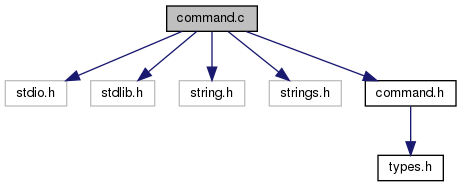
\includegraphics[width=350pt]{command_8c__incl}
\end{center}
\end{figure}
\subsection*{Classes}
\begin{DoxyCompactItemize}
\item 
struct \hyperlink{struct__Comand}{\+\_\+\+Comand}
\end{DoxyCompactItemize}
\subsection*{Macros}
\begin{DoxyCompactItemize}
\item 
\#define \hyperlink{command_8c_a2b1bd24d2eddf8081d8c541e4cc4fd4b}{C\+M\+D\+\_\+\+L\+E\+N\+G\+HT}~30
\item 
\#define \hyperlink{command_8c_ae180fe89f0ae48ce5c80ffaa18de9271}{N\+\_\+\+C\+MD}~12
\end{DoxyCompactItemize}
\subsection*{Functions}
\begin{DoxyCompactItemize}
\item 
\hyperlink{types_8h_a32c27cc471df37f4fc818d65de0a56c4}{S\+T\+A\+T\+US} \hyperlink{command_8c_ab73f9b21268fcb7c4d6918aae58738e7}{comand\+\_\+get\+\_\+user\+\_\+input} (\hyperlink{command_8h_a64fc5834e0580f5f7517e120bd31c301}{Comand} $\ast$comand)
\begin{DoxyCompactList}\small\item\em lee el comando del teclado y si es valido lo ejecuta \end{DoxyCompactList}\item 
\hyperlink{command_8h_a64fc5834e0580f5f7517e120bd31c301}{Comand} $\ast$ \hyperlink{command_8c_aca59ac581052c5503087f1a29b77f8ca}{comand\+\_\+create} ()
\begin{DoxyCompactList}\small\item\em crea un comando definiendo sus campos como U\+N\+K\+N\+O\+WN \end{DoxyCompactList}\item 
void \hyperlink{command_8c_a266fc377d9fa9c814084e4507b006e70}{comand\+\_\+destroy} (\hyperlink{command_8h_a64fc5834e0580f5f7517e120bd31c301}{Comand} $\ast$comand)
\begin{DoxyCompactList}\small\item\em destruye el comando y libera la memoria \end{DoxyCompactList}\item 
\hyperlink{command_8h_a0473597db8c45c0289b6b8e2f8abbe32}{T\+\_\+\+Command} \hyperlink{command_8c_a37c537079e0f082c79bd4a576a8b81d0}{comand\+\_\+get\+\_\+comand} (\hyperlink{command_8h_a64fc5834e0580f5f7517e120bd31c301}{Comand} $\ast$comand)
\begin{DoxyCompactList}\small\item\em devuelve el simbolo del comando que se le pasa \end{DoxyCompactList}\item 
char $\ast$ \hyperlink{command_8c_ab8f45898e8b760f47f7c6a34f1102e6e}{comand\+\_\+get\+\_\+name} (\hyperlink{command_8h_a64fc5834e0580f5f7517e120bd31c301}{Comand} $\ast$comand)
\begin{DoxyCompactList}\small\item\em devuelve el nombre del comando que se le pasa \end{DoxyCompactList}\end{DoxyCompactItemize}
\subsection*{Variables}
\begin{DoxyCompactItemize}
\item 
char $\ast$ \hyperlink{command_8c_aa491d83d4e2f55a3074e418318a8d0fe}{cmd\+\_\+to\+\_\+str} \mbox{[}\hyperlink{command_8c_ae180fe89f0ae48ce5c80ffaa18de9271}{N\+\_\+\+C\+MD}\mbox{]} = \{\char`\"{}No command\char`\"{}, \char`\"{}Unknown\char`\"{}, \char`\"{}Quit\char`\"{}, \char`\"{}Go\char`\"{}, \char`\"{}Take\char`\"{}, \char`\"{}Leave\char`\"{}, \char`\"{}Roll\char`\"{}, \char`\"{}Inspect\char`\"{}, \char`\"{}Following\char`\"{}, \char`\"{}Previous\char`\"{}, \char`\"{}Oca\+\_\+\+Following\char`\"{}, \char`\"{}Oca\+\_\+\+Previous\char`\"{}\}
\item 
char $\ast$ \hyperlink{command_8c_a6397d54c2691d7e8ffe9a8da5db5df58}{short\+\_\+cmd\+\_\+to\+\_\+str} \mbox{[}\hyperlink{command_8c_ae180fe89f0ae48ce5c80ffaa18de9271}{N\+\_\+\+C\+MD}\mbox{]} = \{\char`\"{}\char`\"{}, \char`\"{}\char`\"{}, \char`\"{}q\char`\"{}, \char`\"{}g\char`\"{}, \char`\"{}t\char`\"{}, \char`\"{}l\char`\"{}, \char`\"{}r\char`\"{}, \char`\"{}i\char`\"{}, \char`\"{}f\char`\"{}, \char`\"{}p\char`\"{}, \char`\"{}o\char`\"{}, \char`\"{}a\char`\"{}\}
\end{DoxyCompactItemize}


\subsection{Detailed Description}
En este fichero definimos las funciones para los comandos. 

\begin{DoxyAuthor}{Author}
Manuel Suarez, Saul Almazán, Álvaro Becerra, Rodrigo Lardiés 
\end{DoxyAuthor}
\begin{DoxyVersion}{Version}
3.\+0 
\end{DoxyVersion}
\begin{DoxyDate}{Date}
7/10/2018 
\end{DoxyDate}


\subsection{Macro Definition Documentation}
\mbox{\Hypertarget{command_8c_a2b1bd24d2eddf8081d8c541e4cc4fd4b}\label{command_8c_a2b1bd24d2eddf8081d8c541e4cc4fd4b}} 
\index{command.\+c@{command.\+c}!C\+M\+D\+\_\+\+L\+E\+N\+G\+HT@{C\+M\+D\+\_\+\+L\+E\+N\+G\+HT}}
\index{C\+M\+D\+\_\+\+L\+E\+N\+G\+HT@{C\+M\+D\+\_\+\+L\+E\+N\+G\+HT}!command.\+c@{command.\+c}}
\subsubsection{\texorpdfstring{C\+M\+D\+\_\+\+L\+E\+N\+G\+HT}{CMD\_LENGHT}}
{\footnotesize\ttfamily \#define C\+M\+D\+\_\+\+L\+E\+N\+G\+HT~30}

longitud maxima del comando \mbox{\Hypertarget{command_8c_ae180fe89f0ae48ce5c80ffaa18de9271}\label{command_8c_ae180fe89f0ae48ce5c80ffaa18de9271}} 
\index{command.\+c@{command.\+c}!N\+\_\+\+C\+MD@{N\+\_\+\+C\+MD}}
\index{N\+\_\+\+C\+MD@{N\+\_\+\+C\+MD}!command.\+c@{command.\+c}}
\subsubsection{\texorpdfstring{N\+\_\+\+C\+MD}{N\_CMD}}
{\footnotesize\ttfamily \#define N\+\_\+\+C\+MD~12}

Tamaño de la cadena 

\subsection{Function Documentation}
\mbox{\Hypertarget{command_8c_aca59ac581052c5503087f1a29b77f8ca}\label{command_8c_aca59ac581052c5503087f1a29b77f8ca}} 
\index{command.\+c@{command.\+c}!comand\+\_\+create@{comand\+\_\+create}}
\index{comand\+\_\+create@{comand\+\_\+create}!command.\+c@{command.\+c}}
\subsubsection{\texorpdfstring{comand\+\_\+create()}{comand\_create()}}
{\footnotesize\ttfamily \hyperlink{command_8h_a64fc5834e0580f5f7517e120bd31c301}{Comand}$\ast$ comand\+\_\+create (\begin{DoxyParamCaption}{ }\end{DoxyParamCaption})}



crea un comando definiendo sus campos como U\+N\+K\+N\+O\+WN 

\begin{DoxyAuthor}{Author}
Manuel Suarez, Saul Almazán, Álvaro Becerra, Rodrigo Lardiés 
\end{DoxyAuthor}
\begin{DoxyDate}{Date}
10/11/2018 
\end{DoxyDate}
\begin{DoxyReturn}{Returns}
comand$\ast$ (el comando creado) 
\end{DoxyReturn}
\mbox{\Hypertarget{command_8c_a266fc377d9fa9c814084e4507b006e70}\label{command_8c_a266fc377d9fa9c814084e4507b006e70}} 
\index{command.\+c@{command.\+c}!comand\+\_\+destroy@{comand\+\_\+destroy}}
\index{comand\+\_\+destroy@{comand\+\_\+destroy}!command.\+c@{command.\+c}}
\subsubsection{\texorpdfstring{comand\+\_\+destroy()}{comand\_destroy()}}
{\footnotesize\ttfamily void comand\+\_\+destroy (\begin{DoxyParamCaption}\item[{\hyperlink{command_8h_a64fc5834e0580f5f7517e120bd31c301}{Comand} $\ast$}]{comand }\end{DoxyParamCaption})}



destruye el comando y libera la memoria 

\begin{DoxyAuthor}{Author}
Manuel Suarez, Saul Almazán, Álvaro Becerra, Rodrigo Lardiés 
\end{DoxyAuthor}
\begin{DoxyDate}{Date}
10/11/2018 
\end{DoxyDate}

\begin{DoxyParams}{Parameters}
{\em comand$\ast$} & (el comando que recibe) \\
\hline
\end{DoxyParams}
\begin{DoxyReturn}{Returns}
void (No devuelve nada) 
\end{DoxyReturn}
\mbox{\Hypertarget{command_8c_a37c537079e0f082c79bd4a576a8b81d0}\label{command_8c_a37c537079e0f082c79bd4a576a8b81d0}} 
\index{command.\+c@{command.\+c}!comand\+\_\+get\+\_\+comand@{comand\+\_\+get\+\_\+comand}}
\index{comand\+\_\+get\+\_\+comand@{comand\+\_\+get\+\_\+comand}!command.\+c@{command.\+c}}
\subsubsection{\texorpdfstring{comand\+\_\+get\+\_\+comand()}{comand\_get\_comand()}}
{\footnotesize\ttfamily \hyperlink{command_8h_a0473597db8c45c0289b6b8e2f8abbe32}{T\+\_\+\+Command} comand\+\_\+get\+\_\+comand (\begin{DoxyParamCaption}\item[{\hyperlink{command_8h_a64fc5834e0580f5f7517e120bd31c301}{Comand} $\ast$}]{comand }\end{DoxyParamCaption})}



devuelve el simbolo del comando que se le pasa 

\begin{DoxyAuthor}{Author}
Manuel Suarez, Saul Almazán, Álvaro Becerra, Rodrigo Lardiés 
\end{DoxyAuthor}
\begin{DoxyDate}{Date}
10/11/2018 
\end{DoxyDate}

\begin{DoxyParams}{Parameters}
{\em comand$\ast$} & (el comando que recibe) \\
\hline
\end{DoxyParams}
\begin{DoxyReturn}{Returns}
T\+\_\+\+Command (El simbolo del comando) 
\end{DoxyReturn}
\mbox{\Hypertarget{command_8c_ab8f45898e8b760f47f7c6a34f1102e6e}\label{command_8c_ab8f45898e8b760f47f7c6a34f1102e6e}} 
\index{command.\+c@{command.\+c}!comand\+\_\+get\+\_\+name@{comand\+\_\+get\+\_\+name}}
\index{comand\+\_\+get\+\_\+name@{comand\+\_\+get\+\_\+name}!command.\+c@{command.\+c}}
\subsubsection{\texorpdfstring{comand\+\_\+get\+\_\+name()}{comand\_get\_name()}}
{\footnotesize\ttfamily char$\ast$ comand\+\_\+get\+\_\+name (\begin{DoxyParamCaption}\item[{\hyperlink{command_8h_a64fc5834e0580f5f7517e120bd31c301}{Comand} $\ast$}]{comand }\end{DoxyParamCaption})}



devuelve el nombre del comando que se le pasa 

\begin{DoxyAuthor}{Author}
Manuel Suarez, Saul Almazán, Álvaro Becerra, Rodrigo Lardiés 
\end{DoxyAuthor}
\begin{DoxyDate}{Date}
10/11/2018 
\end{DoxyDate}

\begin{DoxyParams}{Parameters}
{\em comand$\ast$} & (el comando que recibe) \\
\hline
\end{DoxyParams}
\begin{DoxyReturn}{Returns}
char$\ast$ (El nombre del comando) 
\end{DoxyReturn}
\mbox{\Hypertarget{command_8c_ab73f9b21268fcb7c4d6918aae58738e7}\label{command_8c_ab73f9b21268fcb7c4d6918aae58738e7}} 
\index{command.\+c@{command.\+c}!comand\+\_\+get\+\_\+user\+\_\+input@{comand\+\_\+get\+\_\+user\+\_\+input}}
\index{comand\+\_\+get\+\_\+user\+\_\+input@{comand\+\_\+get\+\_\+user\+\_\+input}!command.\+c@{command.\+c}}
\subsubsection{\texorpdfstring{comand\+\_\+get\+\_\+user\+\_\+input()}{comand\_get\_user\_input()}}
{\footnotesize\ttfamily \hyperlink{types_8h_a32c27cc471df37f4fc818d65de0a56c4}{S\+T\+A\+T\+US} comand\+\_\+get\+\_\+user\+\_\+input (\begin{DoxyParamCaption}\item[{\hyperlink{command_8h_a64fc5834e0580f5f7517e120bd31c301}{Comand} $\ast$}]{comand }\end{DoxyParamCaption})}



lee el comando del teclado y si es valido lo ejecuta 

\begin{DoxyAuthor}{Author}
Manuel Suarez, Saul Almazán, Álvaro Becerra, Rodrigo Lardiés 
\end{DoxyAuthor}
\begin{DoxyDate}{Date}
10/11/2018 
\end{DoxyDate}

\begin{DoxyParams}{Parameters}
{\em comand$\ast$} & (el comando que recibe) \\
\hline
\end{DoxyParams}
\begin{DoxyReturn}{Returns}
S\+T\+A\+T\+US (OK si funciona correctamente o E\+R\+R\+OR de lo contrario) 
\end{DoxyReturn}


\subsection{Variable Documentation}
\mbox{\Hypertarget{command_8c_aa491d83d4e2f55a3074e418318a8d0fe}\label{command_8c_aa491d83d4e2f55a3074e418318a8d0fe}} 
\index{command.\+c@{command.\+c}!cmd\+\_\+to\+\_\+str@{cmd\+\_\+to\+\_\+str}}
\index{cmd\+\_\+to\+\_\+str@{cmd\+\_\+to\+\_\+str}!command.\+c@{command.\+c}}
\subsubsection{\texorpdfstring{cmd\+\_\+to\+\_\+str}{cmd\_to\_str}}
{\footnotesize\ttfamily char$\ast$ cmd\+\_\+to\+\_\+str\mbox{[}\hyperlink{command_8c_ae180fe89f0ae48ce5c80ffaa18de9271}{N\+\_\+\+C\+MD}\mbox{]} = \{\char`\"{}No command\char`\"{}, \char`\"{}Unknown\char`\"{}, \char`\"{}Quit\char`\"{}, \char`\"{}Go\char`\"{}, \char`\"{}Take\char`\"{}, \char`\"{}Leave\char`\"{}, \char`\"{}Roll\char`\"{}, \char`\"{}Inspect\char`\"{}, \char`\"{}Following\char`\"{}, \char`\"{}Previous\char`\"{}, \char`\"{}Oca\+\_\+\+Following\char`\"{}, \char`\"{}Oca\+\_\+\+Previous\char`\"{}\}}

Lista de comandos largos \mbox{\Hypertarget{command_8c_a6397d54c2691d7e8ffe9a8da5db5df58}\label{command_8c_a6397d54c2691d7e8ffe9a8da5db5df58}} 
\index{command.\+c@{command.\+c}!short\+\_\+cmd\+\_\+to\+\_\+str@{short\+\_\+cmd\+\_\+to\+\_\+str}}
\index{short\+\_\+cmd\+\_\+to\+\_\+str@{short\+\_\+cmd\+\_\+to\+\_\+str}!command.\+c@{command.\+c}}
\subsubsection{\texorpdfstring{short\+\_\+cmd\+\_\+to\+\_\+str}{short\_cmd\_to\_str}}
{\footnotesize\ttfamily char$\ast$ short\+\_\+cmd\+\_\+to\+\_\+str\mbox{[}\hyperlink{command_8c_ae180fe89f0ae48ce5c80ffaa18de9271}{N\+\_\+\+C\+MD}\mbox{]} = \{\char`\"{}\char`\"{}, \char`\"{}\char`\"{}, \char`\"{}q\char`\"{}, \char`\"{}g\char`\"{}, \char`\"{}t\char`\"{}, \char`\"{}l\char`\"{}, \char`\"{}r\char`\"{}, \char`\"{}i\char`\"{}, \char`\"{}f\char`\"{}, \char`\"{}p\char`\"{}, \char`\"{}o\char`\"{}, \char`\"{}a\char`\"{}\}}

Lista de comandos cortos 
\hypertarget{command__test_8c}{}\section{src/command\+\_\+test.c File Reference}
\label{command__test_8c}\index{src/command\+\_\+test.\+c@{src/command\+\_\+test.\+c}}


Fichero de prueba del comando.  


{\ttfamily \#include $<$stdio.\+h$>$}\newline
{\ttfamily \#include $<$stdlib.\+h$>$}\newline
{\ttfamily \#include $<$string.\+h$>$}\newline
{\ttfamily \#include \char`\"{}types.\+h\char`\"{}}\newline
{\ttfamily \#include \char`\"{}command.\+h\char`\"{}}\newline
Include dependency graph for command\+\_\+test.\+c\+:
% FIG 0
\subsection*{Functions}
\begin{DoxyCompactItemize}
\item 
int \hyperlink{command__test_8c_ae66f6b31b5ad750f1fe042a706a4e3d4}{main} ()
\begin{DoxyCompactList}\small\item\em funcion principal de prueba del comando \end{DoxyCompactList}\end{DoxyCompactItemize}


\subsection{Detailed Description}
Fichero de prueba del comando. 

\begin{DoxyAuthor}{Author}
Manuel Suarez, Saul Almazán, Álvaro Becerra, Rodrigo Lardiés 
\end{DoxyAuthor}
\begin{DoxyVersion}{Version}
1.\+0 
\end{DoxyVersion}
\begin{DoxyDate}{Date}
10/11/2018 
\end{DoxyDate}


\subsection{Function Documentation}
\mbox{\Hypertarget{command__test_8c_ae66f6b31b5ad750f1fe042a706a4e3d4}\label{command__test_8c_ae66f6b31b5ad750f1fe042a706a4e3d4}} 
\index{command\+\_\+test.\+c@{command\+\_\+test.\+c}!main@{main}}
\index{main@{main}!command\+\_\+test.\+c@{command\+\_\+test.\+c}}
\subsubsection{\texorpdfstring{main()}{main()}}
{\footnotesize\ttfamily int main (\begin{DoxyParamCaption}{ }\end{DoxyParamCaption})}



funcion principal de prueba del comando 

\begin{DoxyAuthor}{Author}
Manuel Suarez, Saul Almazán, Álvaro Becerra, Rodrigo Lardiés 
\end{DoxyAuthor}
\begin{DoxyDate}{Date}
10/11/2018 
\end{DoxyDate}
\begin{DoxyReturn}{Returns}
int 
\end{DoxyReturn}

\hypertarget{dialogue_8c}{}\section{src/dialogue.c File Reference}
\label{dialogue_8c}\index{src/dialogue.\+c@{src/dialogue.\+c}}


En este fichero implementamos las funciones del dialogo.  


{\ttfamily \#include $<$stdio.\+h$>$}\newline
{\ttfamily \#include $<$stdlib.\+h$>$}\newline
{\ttfamily \#include $<$string.\+h$>$}\newline
{\ttfamily \#include $<$strings.\+h$>$}\newline
{\ttfamily \#include \char`\"{}types.\+h\char`\"{}}\newline
{\ttfamily \#include \char`\"{}game.\+h\char`\"{}}\newline
{\ttfamily \#include \char`\"{}command.\+h\char`\"{}}\newline
Include dependency graph for dialogue.\+c\+:
% FIG 0
\subsection*{Functions}
\begin{DoxyCompactItemize}
\item 
\hyperlink{types_8h_a32c27cc471df37f4fc818d65de0a56c4}{S\+T\+A\+T\+US} \hyperlink{dialogue_8c_a75c574c3478c2a41ed3b1a11ee70d9ed}{dialogue\+\_\+action} (\hyperlink{command_8h_a7d2935971c252377cb0fc1c8545dc2bc}{Command} $\ast$command, \hyperlink{command_8h_a0473597db8c45c0289b6b8e2f8abbe32}{T\+\_\+\+Command} prev\+\_\+cmd, \hyperlink{types_8h_a32c27cc471df37f4fc818d65de0a56c4}{S\+T\+A\+T\+US} prev\+\_\+stat, \hyperlink{types_8h_a32c27cc471df37f4fc818d65de0a56c4}{S\+T\+A\+T\+US} act\+\_\+stat, char $\ast$aux)
\begin{DoxyCompactList}\small\item\em imprime la descripcion de la acción \end{DoxyCompactList}\end{DoxyCompactItemize}


\subsection{Detailed Description}
En este fichero implementamos las funciones del dialogo. 

\begin{DoxyAuthor}{Author}
Manuel Suarez, Saul Almazán, Álvaro Becerra, Rodrigo Lardiés 
\end{DoxyAuthor}
\begin{DoxyVersion}{Version}
1.\+0 
\end{DoxyVersion}
\begin{DoxyDate}{Date}
16/12/2018 
\end{DoxyDate}


\subsection{Function Documentation}
\mbox{\Hypertarget{dialogue_8c_a75c574c3478c2a41ed3b1a11ee70d9ed}\label{dialogue_8c_a75c574c3478c2a41ed3b1a11ee70d9ed}} 
\index{dialogue.\+c@{dialogue.\+c}!dialogue\+\_\+action@{dialogue\+\_\+action}}
\index{dialogue\+\_\+action@{dialogue\+\_\+action}!dialogue.\+c@{dialogue.\+c}}
\subsubsection{\texorpdfstring{dialogue\+\_\+action()}{dialogue\_action()}}
{\footnotesize\ttfamily \hyperlink{types_8h_a32c27cc471df37f4fc818d65de0a56c4}{S\+T\+A\+T\+US} dialogue\+\_\+action (\begin{DoxyParamCaption}\item[{\hyperlink{command_8h_a7d2935971c252377cb0fc1c8545dc2bc}{Command} $\ast$}]{command,  }\item[{\hyperlink{command_8h_a0473597db8c45c0289b6b8e2f8abbe32}{T\+\_\+\+Command}}]{prev\+\_\+cmd,  }\item[{\hyperlink{types_8h_a32c27cc471df37f4fc818d65de0a56c4}{S\+T\+A\+T\+US}}]{prev\+\_\+stat,  }\item[{\hyperlink{types_8h_a32c27cc471df37f4fc818d65de0a56c4}{S\+T\+A\+T\+US}}]{act\+\_\+stat,  }\item[{char $\ast$}]{aux }\end{DoxyParamCaption})}



imprime la descripcion de la acción 

\begin{DoxyAuthor}{Author}
Manuel Suarez, Saul Almazán, Álvaro Becerra, Rodrigo Lardiés 
\end{DoxyAuthor}
\begin{DoxyDate}{Date}
16/12/2018 
\end{DoxyDate}

\begin{DoxyParams}{Parameters}
{\em command} & comando que se acaba de ejecutar \\
\hline
{\em prev\+\_\+cmd} & comando previo \\
\hline
{\em prev\+\_\+stat} & true si se ha podido ejecutar el comando anterior \\
\hline
{\em act\+\_\+stat} & resultado de la ejecucion del comando \\
\hline
{\em aux} & cadena donde se imprime el resultado \\
\hline
\end{DoxyParams}
\begin{DoxyReturn}{Returns}
OK o E\+R\+R\+OR 
\end{DoxyReturn}

\hypertarget{die_8c}{}\section{src/die.c File Reference}
\label{die_8c}\index{src/die.\+c@{src/die.\+c}}


En este fichero implementamos las funciones del dado.  


{\ttfamily \#include $<$stdio.\+h$>$}\newline
{\ttfamily \#include $<$stdlib.\+h$>$}\newline
{\ttfamily \#include \char`\"{}types.\+h\char`\"{}}\newline
{\ttfamily \#include \char`\"{}die.\+h\char`\"{}}\newline
Include dependency graph for die.\+c\+:
% FIG 0
\subsection*{Classes}
\begin{DoxyCompactItemize}
\item 
struct \hyperlink{struct__Die}{\+\_\+\+Die}
\end{DoxyCompactItemize}
\subsection*{Functions}
\begin{DoxyCompactItemize}
\item 
\hyperlink{die_8h_a892f0b0bf81d69a1f7a14ea238e36dd3}{Die} $\ast$ \hyperlink{die_8c_a7edfb04683a77471c710342df00b7562}{die\+\_\+create} ()
\begin{DoxyCompactList}\small\item\em Crea el dado y devuelve el puntero al mismo. \end{DoxyCompactList}\item 
void \hyperlink{die_8c_a0155d7ec003966bace47f3e032a368e8}{die\+\_\+destroy} (\hyperlink{die_8h_a892f0b0bf81d69a1f7a14ea238e36dd3}{Die} $\ast$die)
\begin{DoxyCompactList}\small\item\em Destruye el dado y libera la memoria. \end{DoxyCompactList}\item 
\hyperlink{types_8h_a32c27cc471df37f4fc818d65de0a56c4}{S\+T\+A\+T\+US} \hyperlink{die_8c_a9062d99f612a9779903e9856c96db9d4}{die\+\_\+set\+\_\+id} (\hyperlink{die_8h_a892f0b0bf81d69a1f7a14ea238e36dd3}{Die} $\ast$die, \hyperlink{types_8h_a845e604fb28f7e3d97549da3448149d3}{Id} id)
\begin{DoxyCompactList}\small\item\em Destruye el dado y libera la memoria. \end{DoxyCompactList}\item 
\hyperlink{types_8h_a845e604fb28f7e3d97549da3448149d3}{Id} \hyperlink{die_8c_a57c9a2627bb3a1ca04fe55d72bd6a5ea}{die\+\_\+get\+\_\+id} (\hyperlink{die_8h_a892f0b0bf81d69a1f7a14ea238e36dd3}{Die} $\ast$die)
\begin{DoxyCompactList}\small\item\em Devuelve el id del dado. \end{DoxyCompactList}\item 
int \hyperlink{die_8c_a9347ed79daba7e8078611d67a52e1bfb}{die\+\_\+get\+\_\+last\+\_\+roll} (\hyperlink{die_8h_a892f0b0bf81d69a1f7a14ea238e36dd3}{Die} $\ast$die)
\begin{DoxyCompactList}\small\item\em Devuelve el resultado obtenido en la anterior tirada. \end{DoxyCompactList}\item 
int \hyperlink{die_8c_a06289514edbedf660c4b043f78e859fc}{die\+\_\+roll} (\hyperlink{die_8h_a892f0b0bf81d69a1f7a14ea238e36dd3}{Die} $\ast$die)
\begin{DoxyCompactList}\small\item\em Tira el dado y devuelve un entero aleatorio entre el inf y el sup. \end{DoxyCompactList}\item 
int \hyperlink{die_8c_adb0fa0ace96ca78efc3c0b191293e005}{die\+\_\+print} (F\+I\+LE $\ast$f, \hyperlink{die_8h_a892f0b0bf81d69a1f7a14ea238e36dd3}{Die} $\ast$die)
\begin{DoxyCompactList}\small\item\em Imprime el valor de la tirada del dado en el archivo proporcionado. \end{DoxyCompactList}\end{DoxyCompactItemize}


\subsection{Detailed Description}
En este fichero implementamos las funciones del dado. 

\begin{DoxyAuthor}{Author}
Manuel Suarez, Saul Almazán, Álvaro Becerra, Rodrigo Lardiés 
\end{DoxyAuthor}
\begin{DoxyVersion}{Version}
1.\+0 
\end{DoxyVersion}
\begin{DoxyDate}{Date}
10/11/2018 
\end{DoxyDate}


\subsection{Function Documentation}
\mbox{\Hypertarget{die_8c_a7edfb04683a77471c710342df00b7562}\label{die_8c_a7edfb04683a77471c710342df00b7562}} 
\index{die.\+c@{die.\+c}!die\+\_\+create@{die\+\_\+create}}
\index{die\+\_\+create@{die\+\_\+create}!die.\+c@{die.\+c}}
\subsubsection{\texorpdfstring{die\+\_\+create()}{die\_create()}}
{\footnotesize\ttfamily \hyperlink{die_8h_a892f0b0bf81d69a1f7a14ea238e36dd3}{Die}$\ast$ die\+\_\+create (\begin{DoxyParamCaption}{ }\end{DoxyParamCaption})}



Crea el dado y devuelve el puntero al mismo. 

\begin{DoxyAuthor}{Author}
Manuel Suarez, Saul Almazán, Álvaro Becerra, Rodrigo Lardiés 
\end{DoxyAuthor}
\begin{DoxyDate}{Date}
10/11/2018 
\end{DoxyDate}
\begin{DoxyReturn}{Returns}
Die (El dado que hemos creado) 
\end{DoxyReturn}
\mbox{\Hypertarget{die_8c_a0155d7ec003966bace47f3e032a368e8}\label{die_8c_a0155d7ec003966bace47f3e032a368e8}} 
\index{die.\+c@{die.\+c}!die\+\_\+destroy@{die\+\_\+destroy}}
\index{die\+\_\+destroy@{die\+\_\+destroy}!die.\+c@{die.\+c}}
\subsubsection{\texorpdfstring{die\+\_\+destroy()}{die\_destroy()}}
{\footnotesize\ttfamily void die\+\_\+destroy (\begin{DoxyParamCaption}\item[{\hyperlink{die_8h_a892f0b0bf81d69a1f7a14ea238e36dd3}{Die} $\ast$}]{die }\end{DoxyParamCaption})}



Destruye el dado y libera la memoria. 

\begin{DoxyAuthor}{Author}
Manuel Suarez, Saul Almazán, Álvaro Becerra, Rodrigo Lardiés 
\end{DoxyAuthor}
\begin{DoxyDate}{Date}
10/11/2018 
\end{DoxyDate}

\begin{DoxyParams}{Parameters}
{\em die} & (puntero a dado) \\
\hline
\end{DoxyParams}
\begin{DoxyReturn}{Returns}
void (No devuelve nada) 
\end{DoxyReturn}
\mbox{\Hypertarget{die_8c_a57c9a2627bb3a1ca04fe55d72bd6a5ea}\label{die_8c_a57c9a2627bb3a1ca04fe55d72bd6a5ea}} 
\index{die.\+c@{die.\+c}!die\+\_\+get\+\_\+id@{die\+\_\+get\+\_\+id}}
\index{die\+\_\+get\+\_\+id@{die\+\_\+get\+\_\+id}!die.\+c@{die.\+c}}
\subsubsection{\texorpdfstring{die\+\_\+get\+\_\+id()}{die\_get\_id()}}
{\footnotesize\ttfamily \hyperlink{types_8h_a845e604fb28f7e3d97549da3448149d3}{Id} die\+\_\+get\+\_\+id (\begin{DoxyParamCaption}\item[{\hyperlink{die_8h_a892f0b0bf81d69a1f7a14ea238e36dd3}{Die} $\ast$}]{die }\end{DoxyParamCaption})}



Devuelve el id del dado. 

\begin{DoxyAuthor}{Author}
Manuel Suarez, Saul Almazán, Álvaro Becerra, Rodrigo Lardiés 
\end{DoxyAuthor}
\begin{DoxyDate}{Date}
10/11/2018 
\end{DoxyDate}

\begin{DoxyParams}{Parameters}
{\em die} & (el dado que vamos a usar) \\
\hline
\end{DoxyParams}
\begin{DoxyReturn}{Returns}
Id (El id del dado) 
\end{DoxyReturn}
\mbox{\Hypertarget{die_8c_a9347ed79daba7e8078611d67a52e1bfb}\label{die_8c_a9347ed79daba7e8078611d67a52e1bfb}} 
\index{die.\+c@{die.\+c}!die\+\_\+get\+\_\+last\+\_\+roll@{die\+\_\+get\+\_\+last\+\_\+roll}}
\index{die\+\_\+get\+\_\+last\+\_\+roll@{die\+\_\+get\+\_\+last\+\_\+roll}!die.\+c@{die.\+c}}
\subsubsection{\texorpdfstring{die\+\_\+get\+\_\+last\+\_\+roll()}{die\_get\_last\_roll()}}
{\footnotesize\ttfamily int die\+\_\+get\+\_\+last\+\_\+roll (\begin{DoxyParamCaption}\item[{\hyperlink{die_8h_a892f0b0bf81d69a1f7a14ea238e36dd3}{Die} $\ast$}]{die }\end{DoxyParamCaption})}



Devuelve el resultado obtenido en la anterior tirada. 

\begin{DoxyAuthor}{Author}
Manuel Suarez, Saul Almazán, Álvaro Becerra, Rodrigo Lardiés 
\end{DoxyAuthor}
\begin{DoxyDate}{Date}
10/11/2018 
\end{DoxyDate}

\begin{DoxyParams}{Parameters}
{\em die} & (el dado que vamos a usar) \\
\hline
\end{DoxyParams}
\begin{DoxyReturn}{Returns}
int (El valor de la tirada) 
\end{DoxyReturn}
\mbox{\Hypertarget{die_8c_adb0fa0ace96ca78efc3c0b191293e005}\label{die_8c_adb0fa0ace96ca78efc3c0b191293e005}} 
\index{die.\+c@{die.\+c}!die\+\_\+print@{die\+\_\+print}}
\index{die\+\_\+print@{die\+\_\+print}!die.\+c@{die.\+c}}
\subsubsection{\texorpdfstring{die\+\_\+print()}{die\_print()}}
{\footnotesize\ttfamily int die\+\_\+print (\begin{DoxyParamCaption}\item[{F\+I\+LE $\ast$}]{f,  }\item[{\hyperlink{die_8h_a892f0b0bf81d69a1f7a14ea238e36dd3}{Die} $\ast$}]{die }\end{DoxyParamCaption})}



Imprime el valor de la tirada del dado en el archivo proporcionado. 

\begin{DoxyAuthor}{Author}
Manuel Suarez, Saul Almazán, Álvaro Becerra, Rodrigo Lardiés 
\end{DoxyAuthor}
\begin{DoxyDate}{Date}
10/11/2018 
\end{DoxyDate}

\begin{DoxyParams}{Parameters}
{\em f} & (El archivo donde lo queremos imprimir) \\
\hline
{\em die} & (el dado que vamos a usar) \\
\hline
\end{DoxyParams}
\begin{DoxyReturn}{Returns}
int (devuelve -\/1 si hay algun error o el un entero en caso contrario) 
\end{DoxyReturn}
\mbox{\Hypertarget{die_8c_a06289514edbedf660c4b043f78e859fc}\label{die_8c_a06289514edbedf660c4b043f78e859fc}} 
\index{die.\+c@{die.\+c}!die\+\_\+roll@{die\+\_\+roll}}
\index{die\+\_\+roll@{die\+\_\+roll}!die.\+c@{die.\+c}}
\subsubsection{\texorpdfstring{die\+\_\+roll()}{die\_roll()}}
{\footnotesize\ttfamily int die\+\_\+roll (\begin{DoxyParamCaption}\item[{\hyperlink{die_8h_a892f0b0bf81d69a1f7a14ea238e36dd3}{Die} $\ast$}]{die }\end{DoxyParamCaption})}



Tira el dado y devuelve un entero aleatorio entre el inf y el sup. 

\begin{DoxyAuthor}{Author}
Manuel Suarez, Saul Almazán, Álvaro Becerra, Rodrigo Lardiés 
\end{DoxyAuthor}
\begin{DoxyDate}{Date}
10/11/2018 
\end{DoxyDate}

\begin{DoxyParams}{Parameters}
{\em die} & (el dado que vamos a usar) \\
\hline
\end{DoxyParams}
\begin{DoxyReturn}{Returns}
int (El valor de la tirada) 
\end{DoxyReturn}
\mbox{\Hypertarget{die_8c_a9062d99f612a9779903e9856c96db9d4}\label{die_8c_a9062d99f612a9779903e9856c96db9d4}} 
\index{die.\+c@{die.\+c}!die\+\_\+set\+\_\+id@{die\+\_\+set\+\_\+id}}
\index{die\+\_\+set\+\_\+id@{die\+\_\+set\+\_\+id}!die.\+c@{die.\+c}}
\subsubsection{\texorpdfstring{die\+\_\+set\+\_\+id()}{die\_set\_id()}}
{\footnotesize\ttfamily \hyperlink{types_8h_a32c27cc471df37f4fc818d65de0a56c4}{S\+T\+A\+T\+US} die\+\_\+set\+\_\+id (\begin{DoxyParamCaption}\item[{\hyperlink{die_8h_a892f0b0bf81d69a1f7a14ea238e36dd3}{Die} $\ast$}]{die,  }\item[{\hyperlink{types_8h_a845e604fb28f7e3d97549da3448149d3}{Id}}]{id }\end{DoxyParamCaption})}



Destruye el dado y libera la memoria. 

\begin{DoxyAuthor}{Author}
Manuel Suarez, Saul Almazán, Álvaro Becerra, Rodrigo Lardiés 
\end{DoxyAuthor}
\begin{DoxyDate}{Date}
10/11/2018 
\end{DoxyDate}

\begin{DoxyParams}{Parameters}
{\em die} & (el dado que vamos a usar) \\
\hline
{\em id} & (el que sera el id del dado) \\
\hline
\end{DoxyParams}
\begin{DoxyReturn}{Returns}
S\+T\+A\+T\+US (OK si funciona correctamente o E\+R\+R\+OR si no) 
\end{DoxyReturn}

\hypertarget{die__test_8c}{}\section{src/die\+\_\+test.c File Reference}
\label{die__test_8c}\index{src/die\+\_\+test.\+c@{src/die\+\_\+test.\+c}}


Prueba del modulo die.  


{\ttfamily \#include $<$stdio.\+h$>$}\newline
{\ttfamily \#include $<$stdlib.\+h$>$}\newline
{\ttfamily \#include $<$string.\+h$>$}\newline
{\ttfamily \#include \char`\"{}die.\+h\char`\"{}}\newline
{\ttfamily \#include \char`\"{}die\+\_\+test.\+h\char`\"{}}\newline
{\ttfamily \#include \char`\"{}test.\+h\char`\"{}}\newline
Include dependency graph for die\+\_\+test.\+c\+:
% FIG 0
\subsection*{Macros}
\begin{DoxyCompactItemize}
\item 
\#define \hyperlink{die__test_8c_a2a77d2f2c5b698c69c19e1f8782bf709}{M\+A\+X\+\_\+\+T\+E\+S\+TS}~9
\end{DoxyCompactItemize}
\subsection*{Functions}
\begin{DoxyCompactItemize}
\item 
int \hyperlink{die__test_8c_a3c04138a5bfe5d72780bb7e82a18e627}{main} (int argc, char $\ast$$\ast$argv)
\begin{DoxyCompactList}\small\item\em Funcion principal de pruebas para el modulo die. \end{DoxyCompactList}\item 
void \hyperlink{die__test_8c_ac0b610468bd3d3b358051c966b771431}{test1\+\_\+die\+\_\+create} ()
\item 
void \hyperlink{die__test_8c_a35fcde570292ad4ff9a876b5e2a2d3f3}{test1\+\_\+die\+\_\+set\+\_\+id} ()
\item 
void \hyperlink{die__test_8c_a7d829d0cae947aad0bc21ded843bd9ab}{test2\+\_\+die\+\_\+set\+\_\+id} ()
\item 
void \hyperlink{die__test_8c_ad27d80a80c4b4fa108337135d5633c90}{test1\+\_\+die\+\_\+get\+\_\+id} ()
\item 
void \hyperlink{die__test_8c_a9c76572bbb86ca9138b99a010e6a184a}{test2\+\_\+die\+\_\+get\+\_\+id} ()
\item 
void \hyperlink{die__test_8c_ac005cb42fa33b38a79896934a5a50001}{test1\+\_\+die\+\_\+roll} ()
\item 
void \hyperlink{die__test_8c_af7df60d905acf9505f1e434c6f75d027}{test2\+\_\+die\+\_\+roll} ()
\item 
void \hyperlink{die__test_8c_a99e873ecce6a19186919e991876dadbe}{test1\+\_\+die\+\_\+get\+\_\+last\+\_\+roll} ()
\item 
void \hyperlink{die__test_8c_a0832aa306964705770b2f1240763d962}{test2\+\_\+die\+\_\+get\+\_\+last\+\_\+roll} ()
\end{DoxyCompactItemize}


\subsection{Detailed Description}
Prueba del modulo die. 

\begin{DoxyAuthor}{Author}
Manuel Suarez, Saul Almazán, �?lvaro Becerra, Rodrigo Lardiés 
\end{DoxyAuthor}
\begin{DoxyVersion}{Version}
1.\+0 
\end{DoxyVersion}
\begin{DoxyDate}{Date}
12-\/11-\/2018 
\end{DoxyDate}


\subsection{Macro Definition Documentation}
\mbox{\Hypertarget{die__test_8c_a2a77d2f2c5b698c69c19e1f8782bf709}\label{die__test_8c_a2a77d2f2c5b698c69c19e1f8782bf709}} 
\index{die\+\_\+test.\+c@{die\+\_\+test.\+c}!M\+A\+X\+\_\+\+T\+E\+S\+TS@{M\+A\+X\+\_\+\+T\+E\+S\+TS}}
\index{M\+A\+X\+\_\+\+T\+E\+S\+TS@{M\+A\+X\+\_\+\+T\+E\+S\+TS}!die\+\_\+test.\+c@{die\+\_\+test.\+c}}
\subsubsection{\texorpdfstring{M\+A\+X\+\_\+\+T\+E\+S\+TS}{MAX\_TESTS}}
{\footnotesize\ttfamily \#define M\+A\+X\+\_\+\+T\+E\+S\+TS~9}

M\+A\+X\+\_\+\+T\+E\+S\+TS 

\subsection{Function Documentation}
\mbox{\Hypertarget{die__test_8c_a3c04138a5bfe5d72780bb7e82a18e627}\label{die__test_8c_a3c04138a5bfe5d72780bb7e82a18e627}} 
\index{die\+\_\+test.\+c@{die\+\_\+test.\+c}!main@{main}}
\index{main@{main}!die\+\_\+test.\+c@{die\+\_\+test.\+c}}
\subsubsection{\texorpdfstring{main()}{main()}}
{\footnotesize\ttfamily int main (\begin{DoxyParamCaption}\item[{int}]{argc,  }\item[{char $\ast$$\ast$}]{argv }\end{DoxyParamCaption})}



Funcion principal de pruebas para el modulo die. 

Dos modos de ejecucion\+: 1.-\/\+Si se ejecuta sin parametros se ejecutan todas las pruebas 2.-\/\+Si se ejecuta con un numero entre 1 y el numero de pruebas solo ejecuta la prueba indicada \mbox{\Hypertarget{die__test_8c_ac0b610468bd3d3b358051c966b771431}\label{die__test_8c_ac0b610468bd3d3b358051c966b771431}} 
\index{die\+\_\+test.\+c@{die\+\_\+test.\+c}!test1\+\_\+die\+\_\+create@{test1\+\_\+die\+\_\+create}}
\index{test1\+\_\+die\+\_\+create@{test1\+\_\+die\+\_\+create}!die\+\_\+test.\+c@{die\+\_\+test.\+c}}
\subsubsection{\texorpdfstring{test1\+\_\+die\+\_\+create()}{test1\_die\_create()}}
{\footnotesize\ttfamily void test1\+\_\+die\+\_\+create (\begin{DoxyParamCaption}{ }\end{DoxyParamCaption})}

\begin{DoxyRefDesc}{Test}
\item[\hyperlink{test__test000001}{Test}]Prueba la función de creación de un dado \end{DoxyRefDesc}
\begin{DoxyPrecond}{Precondition}
nada 
\end{DoxyPrecond}
\begin{DoxyPostcond}{Postcondition}
Un puntero no nulo al dado creado 
\end{DoxyPostcond}
\mbox{\Hypertarget{die__test_8c_ad27d80a80c4b4fa108337135d5633c90}\label{die__test_8c_ad27d80a80c4b4fa108337135d5633c90}} 
\index{die\+\_\+test.\+c@{die\+\_\+test.\+c}!test1\+\_\+die\+\_\+get\+\_\+id@{test1\+\_\+die\+\_\+get\+\_\+id}}
\index{test1\+\_\+die\+\_\+get\+\_\+id@{test1\+\_\+die\+\_\+get\+\_\+id}!die\+\_\+test.\+c@{die\+\_\+test.\+c}}
\subsubsection{\texorpdfstring{test1\+\_\+die\+\_\+get\+\_\+id()}{test1\_die\_get\_id()}}
{\footnotesize\ttfamily void test1\+\_\+die\+\_\+get\+\_\+id (\begin{DoxyParamCaption}{ }\end{DoxyParamCaption})}

\begin{DoxyRefDesc}{Test}
\item[\hyperlink{test__test000004}{Test}]Prueba la función para obtener el id de un dado \end{DoxyRefDesc}
\begin{DoxyPrecond}{Precondition}
El dado tiene id 
\end{DoxyPrecond}
\begin{DoxyPostcond}{Postcondition}
La salida debe ser id=1 
\end{DoxyPostcond}
\mbox{\Hypertarget{die__test_8c_a99e873ecce6a19186919e991876dadbe}\label{die__test_8c_a99e873ecce6a19186919e991876dadbe}} 
\index{die\+\_\+test.\+c@{die\+\_\+test.\+c}!test1\+\_\+die\+\_\+get\+\_\+last\+\_\+roll@{test1\+\_\+die\+\_\+get\+\_\+last\+\_\+roll}}
\index{test1\+\_\+die\+\_\+get\+\_\+last\+\_\+roll@{test1\+\_\+die\+\_\+get\+\_\+last\+\_\+roll}!die\+\_\+test.\+c@{die\+\_\+test.\+c}}
\subsubsection{\texorpdfstring{test1\+\_\+die\+\_\+get\+\_\+last\+\_\+roll()}{test1\_die\_get\_last\_roll()}}
{\footnotesize\ttfamily void test1\+\_\+die\+\_\+get\+\_\+last\+\_\+roll (\begin{DoxyParamCaption}{ }\end{DoxyParamCaption})}

\begin{DoxyRefDesc}{Test}
\item[\hyperlink{test__test000008}{Test}]Prueba la función para obtener la tirada de un dado \end{DoxyRefDesc}
\begin{DoxyPrecond}{Precondition}
dado no N\+U\+LL 
\end{DoxyPrecond}
\begin{DoxyPostcond}{Postcondition}
La salida debe ser $>$0 
\end{DoxyPostcond}
\mbox{\Hypertarget{die__test_8c_ac005cb42fa33b38a79896934a5a50001}\label{die__test_8c_ac005cb42fa33b38a79896934a5a50001}} 
\index{die\+\_\+test.\+c@{die\+\_\+test.\+c}!test1\+\_\+die\+\_\+roll@{test1\+\_\+die\+\_\+roll}}
\index{test1\+\_\+die\+\_\+roll@{test1\+\_\+die\+\_\+roll}!die\+\_\+test.\+c@{die\+\_\+test.\+c}}
\subsubsection{\texorpdfstring{test1\+\_\+die\+\_\+roll()}{test1\_die\_roll()}}
{\footnotesize\ttfamily void test1\+\_\+die\+\_\+roll (\begin{DoxyParamCaption}{ }\end{DoxyParamCaption})}

\begin{DoxyRefDesc}{Test}
\item[\hyperlink{test__test000006}{Test}]Prueba la función para tirar un dado \end{DoxyRefDesc}
\begin{DoxyPrecond}{Precondition}
dado no N\+U\+LL 
\end{DoxyPrecond}
\begin{DoxyPostcond}{Postcondition}
La salida debe ser $>$0 
\end{DoxyPostcond}
\mbox{\Hypertarget{die__test_8c_a35fcde570292ad4ff9a876b5e2a2d3f3}\label{die__test_8c_a35fcde570292ad4ff9a876b5e2a2d3f3}} 
\index{die\+\_\+test.\+c@{die\+\_\+test.\+c}!test1\+\_\+die\+\_\+set\+\_\+id@{test1\+\_\+die\+\_\+set\+\_\+id}}
\index{test1\+\_\+die\+\_\+set\+\_\+id@{test1\+\_\+die\+\_\+set\+\_\+id}!die\+\_\+test.\+c@{die\+\_\+test.\+c}}
\subsubsection{\texorpdfstring{test1\+\_\+die\+\_\+set\+\_\+id()}{test1\_die\_set\_id()}}
{\footnotesize\ttfamily void test1\+\_\+die\+\_\+set\+\_\+id (\begin{DoxyParamCaption}{ }\end{DoxyParamCaption})}

\begin{DoxyRefDesc}{Test}
\item[\hyperlink{test__test000002}{Test}]Prueba la función para establecer un id en el dado \end{DoxyRefDesc}
\begin{DoxyPrecond}{Precondition}
dado no N\+U\+LL e id 
\end{DoxyPrecond}
\begin{DoxyPostcond}{Postcondition}
La salida debe ser OK 
\end{DoxyPostcond}
\mbox{\Hypertarget{die__test_8c_a9c76572bbb86ca9138b99a010e6a184a}\label{die__test_8c_a9c76572bbb86ca9138b99a010e6a184a}} 
\index{die\+\_\+test.\+c@{die\+\_\+test.\+c}!test2\+\_\+die\+\_\+get\+\_\+id@{test2\+\_\+die\+\_\+get\+\_\+id}}
\index{test2\+\_\+die\+\_\+get\+\_\+id@{test2\+\_\+die\+\_\+get\+\_\+id}!die\+\_\+test.\+c@{die\+\_\+test.\+c}}
\subsubsection{\texorpdfstring{test2\+\_\+die\+\_\+get\+\_\+id()}{test2\_die\_get\_id()}}
{\footnotesize\ttfamily void test2\+\_\+die\+\_\+get\+\_\+id (\begin{DoxyParamCaption}{ }\end{DoxyParamCaption})}

\begin{DoxyRefDesc}{Test}
\item[\hyperlink{test__test000005}{Test}]Prueba la función para obtener el id de un dado \end{DoxyRefDesc}
\begin{DoxyPrecond}{Precondition}
El dado es N\+U\+LL 
\end{DoxyPrecond}
\begin{DoxyPostcond}{Postcondition}
La salida debe ser -\/1 
\end{DoxyPostcond}
\mbox{\Hypertarget{die__test_8c_a0832aa306964705770b2f1240763d962}\label{die__test_8c_a0832aa306964705770b2f1240763d962}} 
\index{die\+\_\+test.\+c@{die\+\_\+test.\+c}!test2\+\_\+die\+\_\+get\+\_\+last\+\_\+roll@{test2\+\_\+die\+\_\+get\+\_\+last\+\_\+roll}}
\index{test2\+\_\+die\+\_\+get\+\_\+last\+\_\+roll@{test2\+\_\+die\+\_\+get\+\_\+last\+\_\+roll}!die\+\_\+test.\+c@{die\+\_\+test.\+c}}
\subsubsection{\texorpdfstring{test2\+\_\+die\+\_\+get\+\_\+last\+\_\+roll()}{test2\_die\_get\_last\_roll()}}
{\footnotesize\ttfamily void test2\+\_\+die\+\_\+get\+\_\+last\+\_\+roll (\begin{DoxyParamCaption}{ }\end{DoxyParamCaption})}

\begin{DoxyRefDesc}{Test}
\item[\hyperlink{test__test000009}{Test}]Prueba la función para obtener la tirada de un dado \end{DoxyRefDesc}
\begin{DoxyPrecond}{Precondition}
El dado es N\+U\+LL 
\end{DoxyPrecond}
\begin{DoxyPostcond}{Postcondition}
La salida debe ser -\/1 
\end{DoxyPostcond}
\mbox{\Hypertarget{die__test_8c_af7df60d905acf9505f1e434c6f75d027}\label{die__test_8c_af7df60d905acf9505f1e434c6f75d027}} 
\index{die\+\_\+test.\+c@{die\+\_\+test.\+c}!test2\+\_\+die\+\_\+roll@{test2\+\_\+die\+\_\+roll}}
\index{test2\+\_\+die\+\_\+roll@{test2\+\_\+die\+\_\+roll}!die\+\_\+test.\+c@{die\+\_\+test.\+c}}
\subsubsection{\texorpdfstring{test2\+\_\+die\+\_\+roll()}{test2\_die\_roll()}}
{\footnotesize\ttfamily void test2\+\_\+die\+\_\+roll (\begin{DoxyParamCaption}{ }\end{DoxyParamCaption})}

\begin{DoxyRefDesc}{Test}
\item[\hyperlink{test__test000007}{Test}]Prueba la función para tirar un dado \end{DoxyRefDesc}
\begin{DoxyPrecond}{Precondition}
El dado es N\+U\+LL 
\end{DoxyPrecond}
\begin{DoxyPostcond}{Postcondition}
La salida debe ser -\/1 
\end{DoxyPostcond}
\mbox{\Hypertarget{die__test_8c_a7d829d0cae947aad0bc21ded843bd9ab}\label{die__test_8c_a7d829d0cae947aad0bc21ded843bd9ab}} 
\index{die\+\_\+test.\+c@{die\+\_\+test.\+c}!test2\+\_\+die\+\_\+set\+\_\+id@{test2\+\_\+die\+\_\+set\+\_\+id}}
\index{test2\+\_\+die\+\_\+set\+\_\+id@{test2\+\_\+die\+\_\+set\+\_\+id}!die\+\_\+test.\+c@{die\+\_\+test.\+c}}
\subsubsection{\texorpdfstring{test2\+\_\+die\+\_\+set\+\_\+id()}{test2\_die\_set\_id()}}
{\footnotesize\ttfamily void test2\+\_\+die\+\_\+set\+\_\+id (\begin{DoxyParamCaption}{ }\end{DoxyParamCaption})}

\begin{DoxyRefDesc}{Test}
\item[\hyperlink{test__test000003}{Test}]Prueba la función para establecer un id en el dado \end{DoxyRefDesc}
\begin{DoxyPrecond}{Precondition}
dado N\+U\+LL 
\end{DoxyPrecond}
\begin{DoxyPostcond}{Postcondition}
La salida debe ser E\+R\+R\+OR 
\end{DoxyPostcond}

\hypertarget{game_8c}{}\section{src/game.c File Reference}
\label{game_8c}\index{src/game.\+c@{src/game.\+c}}


En este fichero definimos las funciones para el juego.  


{\ttfamily \#include $<$stdio.\+h$>$}\newline
{\ttfamily \#include $<$stdlib.\+h$>$}\newline
{\ttfamily \#include $<$string.\+h$>$}\newline
{\ttfamily \#include $<$strings.\+h$>$}\newline
{\ttfamily \#include \char`\"{}game.\+h\char`\"{}}\newline
{\ttfamily \#include \char`\"{}game\+\_\+management.\+h\char`\"{}}\newline
Include dependency graph for game.\+c\+:
% FIG 0
\subsection*{Classes}
\begin{DoxyCompactItemize}
\item 
struct \hyperlink{struct__Game}{\+\_\+\+Game}
\end{DoxyCompactItemize}
\subsection*{Functions}
\begin{DoxyCompactItemize}
\item 
\hyperlink{types_8h_a32c27cc471df37f4fc818d65de0a56c4}{S\+T\+A\+T\+US} \hyperlink{game_8c_a39a8bb0b9b5eee8124f56573df4b77f8}{game\+\_\+callback\+\_\+unknown} (\hyperlink{game_8h_a57156d39c530aec3fba3a9dad8c2dc6a}{Game} $\ast$game)
\begin{DoxyCompactList}\small\item\em devuelve el estado tras usar el comando correspondiente \end{DoxyCompactList}\item 
\hyperlink{types_8h_a32c27cc471df37f4fc818d65de0a56c4}{S\+T\+A\+T\+US} \hyperlink{game_8c_ab95080d04cabbb7a7aecc4e9d15ba955}{game\+\_\+callback\+\_\+exit} (\hyperlink{game_8h_a57156d39c530aec3fba3a9dad8c2dc6a}{Game} $\ast$game)
\begin{DoxyCompactList}\small\item\em devuelve el estado tras usar el comando correspondiente \end{DoxyCompactList}\item 
\hyperlink{types_8h_a32c27cc471df37f4fc818d65de0a56c4}{S\+T\+A\+T\+US} \hyperlink{game_8c_a345ceb07363734968ec06f4e3c5bc151}{game\+\_\+callback\+\_\+following} (\hyperlink{game_8h_a57156d39c530aec3fba3a9dad8c2dc6a}{Game} $\ast$game)
\begin{DoxyCompactList}\small\item\em devuelve el estado tras usar el comando correspondiente \end{DoxyCompactList}\item 
\hyperlink{types_8h_a32c27cc471df37f4fc818d65de0a56c4}{S\+T\+A\+T\+US} \hyperlink{game_8c_a4a1423fbc85272706b1d8f271af463f5}{game\+\_\+callback\+\_\+previous} (\hyperlink{game_8h_a57156d39c530aec3fba3a9dad8c2dc6a}{Game} $\ast$game)
\begin{DoxyCompactList}\small\item\em devuelve el estado tras usar el comando correspondiente \end{DoxyCompactList}\item 
\hyperlink{types_8h_a32c27cc471df37f4fc818d65de0a56c4}{S\+T\+A\+T\+US} \hyperlink{game_8c_a45f87a58ee62b8480f1c9357fa7d60d6}{game\+\_\+callback\+\_\+oca\+\_\+following} (\hyperlink{game_8h_a57156d39c530aec3fba3a9dad8c2dc6a}{Game} $\ast$game)
\begin{DoxyCompactList}\small\item\em devuelve el estado tras usar el comando correspondiente \end{DoxyCompactList}\item 
\hyperlink{types_8h_a32c27cc471df37f4fc818d65de0a56c4}{S\+T\+A\+T\+US} \hyperlink{game_8c_aaaf5631832a312665d47ceee9c45c036}{game\+\_\+callback\+\_\+oca\+\_\+previous} (\hyperlink{game_8h_a57156d39c530aec3fba3a9dad8c2dc6a}{Game} $\ast$game)
\begin{DoxyCompactList}\small\item\em devuelve el estado tras usar el comando correspondiente \end{DoxyCompactList}\item 
\hyperlink{types_8h_a32c27cc471df37f4fc818d65de0a56c4}{S\+T\+A\+T\+US} \hyperlink{game_8c_af1e4532ab119c8725df42d2b7295d056}{game\+\_\+callback\+\_\+take\+\_\+object} (\hyperlink{game_8h_a57156d39c530aec3fba3a9dad8c2dc6a}{Game} $\ast$game, \hyperlink{command_8h_a7d2935971c252377cb0fc1c8545dc2bc}{Command} $\ast$cmd)
\begin{DoxyCompactList}\small\item\em devuelve el estado tras usar el comando correspondiente \end{DoxyCompactList}\item 
\hyperlink{types_8h_a32c27cc471df37f4fc818d65de0a56c4}{S\+T\+A\+T\+US} \hyperlink{game_8c_a10e98ae8bcaf37894527d7d930249fb5}{game\+\_\+callback\+\_\+leave\+\_\+object} (\hyperlink{game_8h_a57156d39c530aec3fba3a9dad8c2dc6a}{Game} $\ast$game, \hyperlink{command_8h_a7d2935971c252377cb0fc1c8545dc2bc}{Command} $\ast$cmd)
\begin{DoxyCompactList}\small\item\em devuelve el estado tras usar el comando correspondiente \end{DoxyCompactList}\item 
\hyperlink{types_8h_a32c27cc471df37f4fc818d65de0a56c4}{S\+T\+A\+T\+US} \hyperlink{game_8c_a5796486bc9d6b856b83f6b5829167b35}{game\+\_\+callback\+\_\+roll} (\hyperlink{game_8h_a57156d39c530aec3fba3a9dad8c2dc6a}{Game} $\ast$game)
\begin{DoxyCompactList}\small\item\em devuelve el estado tras usar el comando correspondiente \end{DoxyCompactList}\item 
\hyperlink{types_8h_a32c27cc471df37f4fc818d65de0a56c4}{S\+T\+A\+T\+US} \hyperlink{game_8c_ad9f1ed1530e32e52af6f9a509591f758}{game\+\_\+callback\+\_\+inspect} (\hyperlink{game_8h_a57156d39c530aec3fba3a9dad8c2dc6a}{Game} $\ast$game, \hyperlink{command_8h_a7d2935971c252377cb0fc1c8545dc2bc}{Command} $\ast$cmd)
\begin{DoxyCompactList}\small\item\em devuelve el estado tras usar el comando correspondiente \end{DoxyCompactList}\item 
\hyperlink{types_8h_a32c27cc471df37f4fc818d65de0a56c4}{S\+T\+A\+T\+US} \hyperlink{game_8c_a8d84897e33aa6553c3ec0f79a8f17c94}{game\+\_\+callback\+\_\+go} (\hyperlink{game_8h_a57156d39c530aec3fba3a9dad8c2dc6a}{Game} $\ast$game, \hyperlink{command_8h_a7d2935971c252377cb0fc1c8545dc2bc}{Command} $\ast$cmd)
\begin{DoxyCompactList}\small\item\em devuelve el estado tras usar el comando correspondiente \end{DoxyCompactList}\item 
\hyperlink{types_8h_a32c27cc471df37f4fc818d65de0a56c4}{S\+T\+A\+T\+US} \hyperlink{game_8c_a950e08d948ac357c69205aa1b2b6c402}{game\+\_\+callback\+\_\+turnon} (\hyperlink{game_8h_a57156d39c530aec3fba3a9dad8c2dc6a}{Game} $\ast$game, \hyperlink{command_8h_a7d2935971c252377cb0fc1c8545dc2bc}{Command} $\ast$cmd)
\begin{DoxyCompactList}\small\item\em devuelve el estado tras usar el commando correspondiente \end{DoxyCompactList}\item 
\hyperlink{types_8h_a32c27cc471df37f4fc818d65de0a56c4}{S\+T\+A\+T\+US} \hyperlink{game_8c_a1ade36a2e6ee047d7bc36c3193726fed}{game\+\_\+callback\+\_\+turnoff} (\hyperlink{game_8h_a57156d39c530aec3fba3a9dad8c2dc6a}{Game} $\ast$game, \hyperlink{command_8h_a7d2935971c252377cb0fc1c8545dc2bc}{Command} $\ast$cmd)
\begin{DoxyCompactList}\small\item\em devuelve el estado tras usar el commando correspondiente \end{DoxyCompactList}\item 
\hyperlink{types_8h_a32c27cc471df37f4fc818d65de0a56c4}{S\+T\+A\+T\+US} \hyperlink{game_8c_a24410c1495e435257d20f8c9100af75a}{game\+\_\+callback\+\_\+open} (\hyperlink{game_8h_a57156d39c530aec3fba3a9dad8c2dc6a}{Game} $\ast$game, \hyperlink{command_8h_a7d2935971c252377cb0fc1c8545dc2bc}{Command} $\ast$cmd)
\begin{DoxyCompactList}\small\item\em abre el espacio \end{DoxyCompactList}\item 
\hyperlink{types_8h_a32c27cc471df37f4fc818d65de0a56c4}{S\+T\+A\+T\+US} \hyperlink{game_8c_ad64f3922a8d5d177465fabb53ac0b674}{game\+\_\+callback\+\_\+load} (\hyperlink{game_8h_a57156d39c530aec3fba3a9dad8c2dc6a}{Game} $\ast$game, \hyperlink{command_8h_a7d2935971c252377cb0fc1c8545dc2bc}{Command} $\ast$cmd)
\begin{DoxyCompactList}\small\item\em carga el juego \end{DoxyCompactList}\item 
\hyperlink{types_8h_a32c27cc471df37f4fc818d65de0a56c4}{S\+T\+A\+T\+US} \hyperlink{game_8c_ae20412cd94773240edf08aab6f49daae}{game\+\_\+callback\+\_\+save} (\hyperlink{game_8h_a57156d39c530aec3fba3a9dad8c2dc6a}{Game} $\ast$game, \hyperlink{command_8h_a7d2935971c252377cb0fc1c8545dc2bc}{Command} $\ast$cmd)
\begin{DoxyCompactList}\small\item\em carga el juego \end{DoxyCompactList}\item 
\hyperlink{types_8h_a32c27cc471df37f4fc818d65de0a56c4}{S\+T\+A\+T\+US} \hyperlink{game_8c_ad2290449c7fc014362a9264ad9d94215}{game\+\_\+callback\+\_\+down} (\hyperlink{game_8h_a57156d39c530aec3fba3a9dad8c2dc6a}{Game} $\ast$game)
\begin{DoxyCompactList}\small\item\em devuelve el estado tras usar el commando correspondiente \end{DoxyCompactList}\item 
\hyperlink{types_8h_a32c27cc471df37f4fc818d65de0a56c4}{S\+T\+A\+T\+US} \hyperlink{game_8c_adfed39b91c95af6214a59f16630e64be}{game\+\_\+callback\+\_\+up} (\hyperlink{game_8h_a57156d39c530aec3fba3a9dad8c2dc6a}{Game} $\ast$game)
\begin{DoxyCompactList}\small\item\em devuelve el estado tras usar el commando correspondiente \end{DoxyCompactList}\item 
\hyperlink{types_8h_a845e604fb28f7e3d97549da3448149d3}{Id} \hyperlink{game_8c_ad2dfd865e2bd2c545a15d33f4d1cf3ae}{game\+\_\+get\+\_\+space\+\_\+id\+\_\+at} (\hyperlink{game_8h_a57156d39c530aec3fba3a9dad8c2dc6a}{Game} $\ast$game, int position)
\begin{DoxyCompactList}\small\item\em devuelve el id del espacio de esa posicion \end{DoxyCompactList}\item 
\hyperlink{game_8h_a57156d39c530aec3fba3a9dad8c2dc6a}{Game} $\ast$ \hyperlink{game_8c_a1cdbe3f06b9bf49eb5e334a22ad3b2b9}{game\+\_\+create} ()
\begin{DoxyCompactList}\small\item\em crea un juego vacio sin jugadores ni objetos \end{DoxyCompactList}\item 
\hyperlink{game_8h_a57156d39c530aec3fba3a9dad8c2dc6a}{Game} $\ast$ \hyperlink{game_8c_a0e225eaf98598147fdfba6fed2ea8f02}{game\+\_\+create\+\_\+from\+\_\+file} (char $\ast$filename)
\begin{DoxyCompactList}\small\item\em crea un juego cargando del archivo los espacios, los jugadores, los objetos \end{DoxyCompactList}\item 
\hyperlink{types_8h_a32c27cc471df37f4fc818d65de0a56c4}{S\+T\+A\+T\+US} \hyperlink{game_8c_a0736924a1235c0e6fe9b6d91c2a12af8}{game\+\_\+destroy} (\hyperlink{game_8h_a57156d39c530aec3fba3a9dad8c2dc6a}{Game} $\ast$game)
\begin{DoxyCompactList}\small\item\em destruye el juego y libera la memoria \end{DoxyCompactList}\item 
\hyperlink{types_8h_a32c27cc471df37f4fc818d65de0a56c4}{S\+T\+A\+T\+US} \hyperlink{game_8c_ad6aa8c4df93e9350eab4da74fd74c2c9}{game\+\_\+destroy\+\_\+for\+\_\+load} (\hyperlink{game_8h_a57156d39c530aec3fba3a9dad8c2dc6a}{Game} $\ast$game)
\begin{DoxyCompactList}\small\item\em destruye el juego para poder cargar otro \end{DoxyCompactList}\item 
\hyperlink{types_8h_a3e5b8192e7d9ffaf3542f1210aec18dd}{B\+O\+OL} \hyperlink{game_8c_aa6efe0650af110bbd84e742cc8046d93}{game\+\_\+is\+\_\+over} (\hyperlink{game_8h_a57156d39c530aec3fba3a9dad8c2dc6a}{Game} $\ast$game)
\begin{DoxyCompactList}\small\item\em En este caso devuelve F\+A\+L\+SE siempre. \end{DoxyCompactList}\item 
\hyperlink{types_8h_a32c27cc471df37f4fc818d65de0a56c4}{S\+T\+A\+T\+US} \hyperlink{game_8c_ae5ad86de0a92d9eccb234948458da7f1}{game\+\_\+add\+\_\+space} (\hyperlink{game_8h_a57156d39c530aec3fba3a9dad8c2dc6a}{Game} $\ast$game, \hyperlink{space_8h_a67533ffc2b70463baecc38fb0629bbfc}{Space} $\ast$space)
\begin{DoxyCompactList}\small\item\em añade un espacio al juego \end{DoxyCompactList}\item 
\hyperlink{types_8h_a32c27cc471df37f4fc818d65de0a56c4}{S\+T\+A\+T\+US} \hyperlink{game_8c_a9597a8e456aa74db536e87d56f56c3b4}{game\+\_\+add\+\_\+object} (\hyperlink{game_8h_a57156d39c530aec3fba3a9dad8c2dc6a}{Game} $\ast$game, \hyperlink{object_8h_a7f8bbcda919b65ce67f92fba08e0212f}{Object} $\ast$object)
\begin{DoxyCompactList}\small\item\em añade un objeto al juego \end{DoxyCompactList}\item 
\hyperlink{types_8h_a32c27cc471df37f4fc818d65de0a56c4}{S\+T\+A\+T\+US} \hyperlink{game_8c_a4691bee17d5784ad6eb257dfbb252c27}{game\+\_\+add\+\_\+link} (\hyperlink{game_8h_a57156d39c530aec3fba3a9dad8c2dc6a}{Game} $\ast$game, \hyperlink{link_8h_ae3b299941e67be6971bfd64a25505eff}{Link} $\ast$link)
\begin{DoxyCompactList}\small\item\em añade un link al juego \end{DoxyCompactList}\item 
\hyperlink{types_8h_a32c27cc471df37f4fc818d65de0a56c4}{S\+T\+A\+T\+US} \hyperlink{game_8c_a4280b7ee7ac0d4575d0aa88e8b7f921b}{game\+\_\+add\+\_\+player} (\hyperlink{game_8h_a57156d39c530aec3fba3a9dad8c2dc6a}{Game} $\ast$game, \hyperlink{player_8h_af30e2030635a69690f85e48bc6ef202f}{Player} $\ast$player)
\begin{DoxyCompactList}\small\item\em añade un jugador al juego \end{DoxyCompactList}\item 
\hyperlink{space_8h_a67533ffc2b70463baecc38fb0629bbfc}{Space} $\ast$ \hyperlink{game_8c_a69d94da9d27b542d3ebdeb8b60f1f2dc}{game\+\_\+get\+\_\+space} (\hyperlink{game_8h_a57156d39c530aec3fba3a9dad8c2dc6a}{Game} $\ast$game, \hyperlink{types_8h_a845e604fb28f7e3d97549da3448149d3}{Id} id)
\begin{DoxyCompactList}\small\item\em devuelve el id de la posicion del jugador \end{DoxyCompactList}\item 
\hyperlink{types_8h_a32c27cc471df37f4fc818d65de0a56c4}{S\+T\+A\+T\+US} \hyperlink{game_8c_aab6da8e0f8986df17362e6acabca3a9d}{game\+\_\+set\+\_\+object\+\_\+location} (\hyperlink{game_8h_a57156d39c530aec3fba3a9dad8c2dc6a}{Game} $\ast$game, \hyperlink{types_8h_a845e604fb28f7e3d97549da3448149d3}{Id} id, \hyperlink{types_8h_a845e604fb28f7e3d97549da3448149d3}{Id} id\+\_\+object)
\begin{DoxyCompactList}\small\item\em modifica la posicion de un objeto \end{DoxyCompactList}\item 
\hyperlink{types_8h_a845e604fb28f7e3d97549da3448149d3}{Id} \hyperlink{game_8c_ac6a628f2106f81c37d0e83c67920615f}{game\+\_\+get\+\_\+player\+\_\+location} (\hyperlink{game_8h_a57156d39c530aec3fba3a9dad8c2dc6a}{Game} $\ast$game)
\begin{DoxyCompactList}\small\item\em devuelve el id de la posicion del jugador \end{DoxyCompactList}\item 
\hyperlink{types_8h_a845e604fb28f7e3d97549da3448149d3}{Id} \hyperlink{game_8c_aa84eca5a1131daafd7acbf74263b6f82}{game\+\_\+get\+\_\+object\+\_\+location} (\hyperlink{game_8h_a57156d39c530aec3fba3a9dad8c2dc6a}{Game} $\ast$game, \hyperlink{types_8h_a845e604fb28f7e3d97549da3448149d3}{Id} id)
\begin{DoxyCompactList}\small\item\em devuelve el id de la posicion del objeto \end{DoxyCompactList}\item 
char $\ast$ \hyperlink{game_8c_a325504cf9558c0f25eae56aa35633941}{game\+\_\+get\+\_\+object\+\_\+name} (\hyperlink{game_8h_a57156d39c530aec3fba3a9dad8c2dc6a}{Game} $\ast$game, \hyperlink{types_8h_a845e604fb28f7e3d97549da3448149d3}{Id} id)
\begin{DoxyCompactList}\small\item\em devuelve el nombre del objeto \end{DoxyCompactList}\item 
char $\ast$ \hyperlink{game_8c_ab9ac0fa0bea1c60a4a120ff2e3238806}{game\+\_\+get\+\_\+player\+\_\+name} (\hyperlink{game_8h_a57156d39c530aec3fba3a9dad8c2dc6a}{Game} $\ast$game)
\begin{DoxyCompactList}\small\item\em devuelve el nombre de un jugador \end{DoxyCompactList}\item 
\hyperlink{types_8h_a32c27cc471df37f4fc818d65de0a56c4}{S\+T\+A\+T\+US} \hyperlink{game_8c_a8cd2183284a5c498af5ed2ae9d42936e}{game\+\_\+string\+\_\+objects\+\_\+localization} (\hyperlink{game_8h_a57156d39c530aec3fba3a9dad8c2dc6a}{Game} $\ast$game, char $\ast$cadena)
\begin{DoxyCompactList}\small\item\em pasa una cadena de objetos al juego \end{DoxyCompactList}\item 
\hyperlink{types_8h_a32c27cc471df37f4fc818d65de0a56c4}{S\+T\+A\+T\+US} \hyperlink{game_8c_a8263cc2e06c6cde8c5a92d485a59eff7}{game\+\_\+string\+\_\+objects} (\hyperlink{game_8h_a57156d39c530aec3fba3a9dad8c2dc6a}{Game} $\ast$game, \hyperlink{space_8h_a67533ffc2b70463baecc38fb0629bbfc}{Space} $\ast$space, char $\ast$cadena)
\begin{DoxyCompactList}\small\item\em pasa una cadena de objetos al juego \end{DoxyCompactList}\item 
\hyperlink{types_8h_a32c27cc471df37f4fc818d65de0a56c4}{S\+T\+A\+T\+US} \hyperlink{game_8c_ac41f5b1aca098e478958f69560118159}{game\+\_\+string\+\_\+objects\+\_\+player} (\hyperlink{game_8h_a57156d39c530aec3fba3a9dad8c2dc6a}{Game} $\ast$game, char $\ast$cadena)
\begin{DoxyCompactList}\small\item\em pasa una cadena de objetos del jugador al juego \end{DoxyCompactList}\item 
int \hyperlink{game_8c_a51cdc1dc9dbb470f51266e19acd17cdf}{game\+\_\+get\+\_\+roll\+\_\+die} (\hyperlink{game_8h_a57156d39c530aec3fba3a9dad8c2dc6a}{Game} $\ast$game)
\begin{DoxyCompactList}\small\item\em tira el dado del juego \end{DoxyCompactList}\item 
\hyperlink{types_8h_a32c27cc471df37f4fc818d65de0a56c4}{S\+T\+A\+T\+US} \hyperlink{game_8c_a0a3e83f8ac4e4a94d6975d776abf27fa}{game\+\_\+update} (\hyperlink{game_8h_a57156d39c530aec3fba3a9dad8c2dc6a}{Game} $\ast$game, \hyperlink{command_8h_a7d2935971c252377cb0fc1c8545dc2bc}{Command} $\ast$command)
\begin{DoxyCompactList}\small\item\em actualiza el juego tras pasarle el commando introducido \end{DoxyCompactList}\item 
\hyperlink{types_8h_a3e5b8192e7d9ffaf3542f1210aec18dd}{B\+O\+OL} \hyperlink{game_8c_ae385e82346561a8306acbd5fbd20fa87}{game\+\_\+player\+\_\+bag\+\_\+is\+\_\+full} (\hyperlink{game_8h_a57156d39c530aec3fba3a9dad8c2dc6a}{Game} $\ast$game)
\begin{DoxyCompactList}\small\item\em Para saber si la mochila del jugador está llena. \end{DoxyCompactList}\item 
\hyperlink{command_8h_a0473597db8c45c0289b6b8e2f8abbe32}{T\+\_\+\+Command} \hyperlink{game_8c_ac35df1afdade2b7659ebbcfeca1f0c35}{game\+\_\+get\+\_\+last\+\_\+command} (\hyperlink{game_8h_a57156d39c530aec3fba3a9dad8c2dc6a}{Game} $\ast$game)
\begin{DoxyCompactList}\small\item\em El ultimo commando usado. \end{DoxyCompactList}\item 
char $\ast$ \hyperlink{game_8c_a3b7fb1aa2ce2db9ed7d9f4b0c9aaeea5}{game\+\_\+get\+\_\+dialogue} (\hyperlink{game_8h_a57156d39c530aec3fba3a9dad8c2dc6a}{Game} $\ast$game)
\begin{DoxyCompactList}\small\item\em se obtiene el diálogo \end{DoxyCompactList}\item 
int \hyperlink{game_8c_a1d0ce9a75987c1515afcb74eccdccc40}{game\+\_\+roll\+\_\+die} (\hyperlink{game_8h_a57156d39c530aec3fba3a9dad8c2dc6a}{Game} $\ast$game)
\begin{DoxyCompactList}\small\item\em se tira el dado \end{DoxyCompactList}\item 
\hyperlink{types_8h_a32c27cc471df37f4fc818d65de0a56c4}{S\+T\+A\+T\+US} \hyperlink{game_8c_a04a732fd155c88606ce407c5fc609171}{game\+\_\+get\+\_\+result\+\_\+last\+\_\+command} (\hyperlink{game_8h_a57156d39c530aec3fba3a9dad8c2dc6a}{Game} $\ast$game)
\begin{DoxyCompactList}\small\item\em devuelve el resultado de introducir el ultimo commando en el juego \end{DoxyCompactList}\item 
\hyperlink{command_8h_a0473597db8c45c0289b6b8e2f8abbe32}{T\+\_\+\+Command} \hyperlink{game_8c_ac304be8aaed3e3d4d3f27f734b096630}{game\+\_\+get\+\_\+prev\+\_\+command} (\hyperlink{game_8h_a57156d39c530aec3fba3a9dad8c2dc6a}{Game} $\ast$game)
\begin{DoxyCompactList}\small\item\em El ultimo commando usado. \end{DoxyCompactList}\item 
\hyperlink{types_8h_a32c27cc471df37f4fc818d65de0a56c4}{S\+T\+A\+T\+US} \hyperlink{game_8c_a65a734fccbc2954e3b4323334a351a20}{game\+\_\+get\+\_\+result\+\_\+prev\+\_\+command} (\hyperlink{game_8h_a57156d39c530aec3fba3a9dad8c2dc6a}{Game} $\ast$game)
\begin{DoxyCompactList}\small\item\em devuelve el resultado de introducir el ultimo commando en el juego \end{DoxyCompactList}\item 
void \hyperlink{game_8c_a33a5ed8937423f8c012df3cedad4fa4c}{game\+\_\+print\+\_\+data} (\hyperlink{game_8h_a57156d39c530aec3fba3a9dad8c2dc6a}{Game} $\ast$game)
\begin{DoxyCompactList}\small\item\em Imprime el juego. \end{DoxyCompactList}\item 
\hyperlink{types_8h_a32c27cc471df37f4fc818d65de0a56c4}{S\+T\+A\+T\+US} \hyperlink{game_8c_a47bcbbfca86c0df6dfea3ce506e73d15}{game\+\_\+change\+\_\+light\+\_\+space} (\hyperlink{game_8h_a57156d39c530aec3fba3a9dad8c2dc6a}{Game} $\ast$game)
\begin{DoxyCompactList}\small\item\em cambia la luz del espacio \end{DoxyCompactList}\item 
\hyperlink{types_8h_a32c27cc471df37f4fc818d65de0a56c4}{S\+T\+A\+T\+US} \hyperlink{game_8c_a9db26a4abdd96e5be50b4ada700b7955}{game\+\_\+close\+\_\+links} (\hyperlink{game_8h_a57156d39c530aec3fba3a9dad8c2dc6a}{Game} $\ast$game)
\begin{DoxyCompactList}\small\item\em cierra un link \end{DoxyCompactList}\item 
\hyperlink{types_8h_a32c27cc471df37f4fc818d65de0a56c4}{S\+T\+A\+T\+US} \hyperlink{game_8c_a9f686c3100433c10b6d8619070940d5d}{game\+\_\+kill\+\_\+player} (\hyperlink{game_8h_a57156d39c530aec3fba3a9dad8c2dc6a}{Game} $\ast$game)
\begin{DoxyCompactList}\small\item\em mata al jugador \end{DoxyCompactList}\item 
\hyperlink{types_8h_a32c27cc471df37f4fc818d65de0a56c4}{S\+T\+A\+T\+US} \hyperlink{game_8c_a36658b5ee83f7924eece6a39bcc0236d}{game\+\_\+appear\+\_\+link} (\hyperlink{game_8h_a57156d39c530aec3fba3a9dad8c2dc6a}{Game} $\ast$game)
\begin{DoxyCompactList}\small\item\em cambia un link \end{DoxyCompactList}\item 
\hyperlink{types_8h_a32c27cc471df37f4fc818d65de0a56c4}{S\+T\+A\+T\+US} \hyperlink{game_8c_a64adeccebb3459663b452cfe5fb2ab61}{game\+\_\+change\+\_\+object\+\_\+location} (\hyperlink{game_8h_a57156d39c530aec3fba3a9dad8c2dc6a}{Game} $\ast$game)
\begin{DoxyCompactList}\small\item\em cambia la localizacion de un objeto \end{DoxyCompactList}\item 
\hyperlink{types_8h_a32c27cc471df37f4fc818d65de0a56c4}{S\+T\+A\+T\+US} \hyperlink{game_8c_a2ab482d4e93cec88ba855c8d74c902f1}{game\+\_\+hide\+\_\+objects} (\hyperlink{game_8h_a57156d39c530aec3fba3a9dad8c2dc6a}{Game} $\ast$game)
\begin{DoxyCompactList}\small\item\em oculta un objeto \end{DoxyCompactList}\item 
char $\ast$ \hyperlink{game_8c_ad7a3c7a3776cf5154f9b2165e92edc21}{game\+\_\+get\+\_\+last\+\_\+description\+\_\+asked} (\hyperlink{game_8h_a57156d39c530aec3fba3a9dad8c2dc6a}{Game} $\ast$game)
\begin{DoxyCompactList}\small\item\em Devuelve la ultima descripcion del juego. \end{DoxyCompactList}\item 
\hyperlink{link_8h_ae3b299941e67be6971bfd64a25505eff}{Link} $\ast$ \hyperlink{game_8c_a08ad17816339cf8c469b2ce213cd06e4}{game\+\_\+get\+\_\+link} (\hyperlink{game_8h_a57156d39c530aec3fba3a9dad8c2dc6a}{Game} $\ast$game, \hyperlink{types_8h_a845e604fb28f7e3d97549da3448149d3}{Id} link\+\_\+id)
\begin{DoxyCompactList}\small\item\em El link de un id pasado como argumento. \end{DoxyCompactList}\item 
\hyperlink{types_8h_a845e604fb28f7e3d97549da3448149d3}{Id} \hyperlink{game_8c_a09a62ede5842bd7b68b9c971f9c99b40}{game\+\_\+get\+\_\+id\+\_\+conected\+\_\+space} (\hyperlink{game_8h_a57156d39c530aec3fba3a9dad8c2dc6a}{Game} $\ast$game, \hyperlink{types_8h_a845e604fb28f7e3d97549da3448149d3}{Id} link\+\_\+id, \hyperlink{types_8h_a845e604fb28f7e3d97549da3448149d3}{Id} space\+\_\+id)
\begin{DoxyCompactList}\small\item\em devuelve el id del espacio conectado \end{DoxyCompactList}\item 
\hyperlink{space_8h_a67533ffc2b70463baecc38fb0629bbfc}{Space} $\ast$ \hyperlink{game_8c_a18ae1a39a979d89d360726ef7dde33bf}{game\+\_\+get\+\_\+space\+\_\+order} (\hyperlink{game_8h_a57156d39c530aec3fba3a9dad8c2dc6a}{Game} $\ast$game, int pos)
\begin{DoxyCompactList}\small\item\em devuelve el espacio de una posicion \end{DoxyCompactList}\item 
\hyperlink{link_8h_ae3b299941e67be6971bfd64a25505eff}{Link} $\ast$ \hyperlink{game_8c_a1cd176918f2066ea1952ebb9ac621acd}{game\+\_\+get\+\_\+link\+\_\+order} (\hyperlink{game_8h_a57156d39c530aec3fba3a9dad8c2dc6a}{Game} $\ast$game, int pos)
\begin{DoxyCompactList}\small\item\em devuelve el link de una posicion \end{DoxyCompactList}\item 
\hyperlink{object_8h_a7f8bbcda919b65ce67f92fba08e0212f}{Object} $\ast$ \hyperlink{game_8c_a615c1585f947226ebd7c23bfefa49eba}{game\+\_\+get\+\_\+object\+\_\+order} (\hyperlink{game_8h_a57156d39c530aec3fba3a9dad8c2dc6a}{Game} $\ast$game, int pos)
\begin{DoxyCompactList}\small\item\em devuelve el objeto de una posicion \end{DoxyCompactList}\item 
\hyperlink{types_8h_a32c27cc471df37f4fc818d65de0a56c4}{S\+T\+A\+T\+US} \hyperlink{game_8c_ad8ff766ce3ed5a90189c46f03f9fe711}{game\+\_\+string\+\_\+object\+\_\+player\+\_\+save} (\hyperlink{game_8h_a57156d39c530aec3fba3a9dad8c2dc6a}{Game} $\ast$game, char $\ast$cadena)
\begin{DoxyCompactList}\small\item\em crea una cadena con los objetos del jugador para guardarla \end{DoxyCompactList}\item 
\hyperlink{player_8h_af30e2030635a69690f85e48bc6ef202f}{Player} $\ast$ \hyperlink{game_8c_af46efd507d797aec6da90d08aa592e32}{game\+\_\+get\+\_\+player} (\hyperlink{game_8h_a57156d39c530aec3fba3a9dad8c2dc6a}{Game} $\ast$game)
\begin{DoxyCompactList}\small\item\em Devuelve un puntero al jugador. \end{DoxyCompactList}\end{DoxyCompactItemize}


\subsection{Detailed Description}
En este fichero definimos las funciones para el juego. 

\begin{DoxyAuthor}{Author}
Manuel Suarez, Saul Almazán, Álvaro Becerra, Rodrigo Lardiés 
\end{DoxyAuthor}
\begin{DoxyVersion}{Version}
3.\+0 
\end{DoxyVersion}
\begin{DoxyDate}{Date}
21/10/2018 
\end{DoxyDate}


\subsection{Function Documentation}
\mbox{\Hypertarget{game_8c_a4691bee17d5784ad6eb257dfbb252c27}\label{game_8c_a4691bee17d5784ad6eb257dfbb252c27}} 
\index{game.\+c@{game.\+c}!game\+\_\+add\+\_\+link@{game\+\_\+add\+\_\+link}}
\index{game\+\_\+add\+\_\+link@{game\+\_\+add\+\_\+link}!game.\+c@{game.\+c}}
\subsubsection{\texorpdfstring{game\+\_\+add\+\_\+link()}{game\_add\_link()}}
{\footnotesize\ttfamily \hyperlink{types_8h_a32c27cc471df37f4fc818d65de0a56c4}{S\+T\+A\+T\+US} game\+\_\+add\+\_\+link (\begin{DoxyParamCaption}\item[{\hyperlink{game_8h_a57156d39c530aec3fba3a9dad8c2dc6a}{Game} $\ast$}]{game,  }\item[{\hyperlink{link_8h_ae3b299941e67be6971bfd64a25505eff}{Link} $\ast$}]{link }\end{DoxyParamCaption})}



añade un link al juego 

\begin{DoxyAuthor}{Author}
Manuel Suarez, Saul Almazán, Álvaro Becerra, Rodrigo Lardiés 
\end{DoxyAuthor}
\begin{DoxyDate}{Date}
10/11/2018 
\end{DoxyDate}

\begin{DoxyParams}{Parameters}
{\em game} & (El juego al que vamos a añadir) \\
\hline
{\em link} & (Lo que vamos a añadir) \\
\hline
\end{DoxyParams}
\begin{DoxyReturn}{Returns}
S\+T\+A\+T\+US (OK si se ha realizado correctamente o E\+R\+R\+OR de lo contrario) 
\end{DoxyReturn}
\mbox{\Hypertarget{game_8c_a9597a8e456aa74db536e87d56f56c3b4}\label{game_8c_a9597a8e456aa74db536e87d56f56c3b4}} 
\index{game.\+c@{game.\+c}!game\+\_\+add\+\_\+object@{game\+\_\+add\+\_\+object}}
\index{game\+\_\+add\+\_\+object@{game\+\_\+add\+\_\+object}!game.\+c@{game.\+c}}
\subsubsection{\texorpdfstring{game\+\_\+add\+\_\+object()}{game\_add\_object()}}
{\footnotesize\ttfamily \hyperlink{types_8h_a32c27cc471df37f4fc818d65de0a56c4}{S\+T\+A\+T\+US} game\+\_\+add\+\_\+object (\begin{DoxyParamCaption}\item[{\hyperlink{game_8h_a57156d39c530aec3fba3a9dad8c2dc6a}{Game} $\ast$}]{game,  }\item[{\hyperlink{object_8h_a7f8bbcda919b65ce67f92fba08e0212f}{Object} $\ast$}]{object }\end{DoxyParamCaption})}



añade un objeto al juego 

\begin{DoxyAuthor}{Author}
Manuel Suarez, Saul Almazán, Álvaro Becerra, Rodrigo Lardiés 
\end{DoxyAuthor}
\begin{DoxyDate}{Date}
10/11/2018 
\end{DoxyDate}

\begin{DoxyParams}{Parameters}
{\em game} & (El juego al que vamos a añadir) \\
\hline
{\em object} & (Lo que vamos a añadir) \\
\hline
\end{DoxyParams}
\begin{DoxyReturn}{Returns}
S\+T\+A\+T\+US (OK si se ha realizado correctamente o E\+R\+R\+OR de lo contrario) 
\end{DoxyReturn}
\mbox{\Hypertarget{game_8c_a4280b7ee7ac0d4575d0aa88e8b7f921b}\label{game_8c_a4280b7ee7ac0d4575d0aa88e8b7f921b}} 
\index{game.\+c@{game.\+c}!game\+\_\+add\+\_\+player@{game\+\_\+add\+\_\+player}}
\index{game\+\_\+add\+\_\+player@{game\+\_\+add\+\_\+player}!game.\+c@{game.\+c}}
\subsubsection{\texorpdfstring{game\+\_\+add\+\_\+player()}{game\_add\_player()}}
{\footnotesize\ttfamily \hyperlink{types_8h_a32c27cc471df37f4fc818d65de0a56c4}{S\+T\+A\+T\+US} game\+\_\+add\+\_\+player (\begin{DoxyParamCaption}\item[{\hyperlink{game_8h_a57156d39c530aec3fba3a9dad8c2dc6a}{Game} $\ast$}]{game,  }\item[{\hyperlink{player_8h_af30e2030635a69690f85e48bc6ef202f}{Player} $\ast$}]{player }\end{DoxyParamCaption})}



añade un jugador al juego 

\begin{DoxyAuthor}{Author}
Manuel Suarez, Saul Almazán, Álvaro Becerra, Rodrigo Lardiés 
\end{DoxyAuthor}
\begin{DoxyDate}{Date}
10/11/2018 
\end{DoxyDate}

\begin{DoxyParams}{Parameters}
{\em game} & (El juego al que vamos a añadir) \\
\hline
{\em player} & (Lo que vamos a añadir) \\
\hline
\end{DoxyParams}
\begin{DoxyReturn}{Returns}
S\+T\+A\+T\+US (OK si se ha realizado correctamente o E\+R\+R\+OR de lo contrario) 
\end{DoxyReturn}
\mbox{\Hypertarget{game_8c_ae5ad86de0a92d9eccb234948458da7f1}\label{game_8c_ae5ad86de0a92d9eccb234948458da7f1}} 
\index{game.\+c@{game.\+c}!game\+\_\+add\+\_\+space@{game\+\_\+add\+\_\+space}}
\index{game\+\_\+add\+\_\+space@{game\+\_\+add\+\_\+space}!game.\+c@{game.\+c}}
\subsubsection{\texorpdfstring{game\+\_\+add\+\_\+space()}{game\_add\_space()}}
{\footnotesize\ttfamily \hyperlink{types_8h_a32c27cc471df37f4fc818d65de0a56c4}{S\+T\+A\+T\+US} game\+\_\+add\+\_\+space (\begin{DoxyParamCaption}\item[{\hyperlink{game_8h_a57156d39c530aec3fba3a9dad8c2dc6a}{Game} $\ast$}]{game,  }\item[{\hyperlink{space_8h_a67533ffc2b70463baecc38fb0629bbfc}{Space} $\ast$}]{space }\end{DoxyParamCaption})}



añade un espacio al juego 

\begin{DoxyAuthor}{Author}
Manuel Suarez, Saul Almazán, Álvaro Becerra, Rodrigo Lardiés 
\end{DoxyAuthor}
\begin{DoxyDate}{Date}
10/11/2018 
\end{DoxyDate}

\begin{DoxyParams}{Parameters}
{\em game} & (El juego al que vamos a añadir) \\
\hline
{\em space} & (Lo que vamos a añadir) \\
\hline
\end{DoxyParams}
\begin{DoxyReturn}{Returns}
S\+T\+A\+T\+US (OK si se ha realizado correctamente o E\+R\+R\+OR de lo contrario) 
\end{DoxyReturn}
\mbox{\Hypertarget{game_8c_a36658b5ee83f7924eece6a39bcc0236d}\label{game_8c_a36658b5ee83f7924eece6a39bcc0236d}} 
\index{game.\+c@{game.\+c}!game\+\_\+appear\+\_\+link@{game\+\_\+appear\+\_\+link}}
\index{game\+\_\+appear\+\_\+link@{game\+\_\+appear\+\_\+link}!game.\+c@{game.\+c}}
\subsubsection{\texorpdfstring{game\+\_\+appear\+\_\+link()}{game\_appear\_link()}}
{\footnotesize\ttfamily \hyperlink{types_8h_a32c27cc471df37f4fc818d65de0a56c4}{S\+T\+A\+T\+US} game\+\_\+appear\+\_\+link (\begin{DoxyParamCaption}\item[{\hyperlink{game_8h_a57156d39c530aec3fba3a9dad8c2dc6a}{Game} $\ast$}]{game }\end{DoxyParamCaption})}



cambia un link 

\begin{DoxyAuthor}{Author}
Manuel Suarez, Saul Almazán, Álvaro Becerra, Rodrigo Lardiés 
\end{DoxyAuthor}
\begin{DoxyDate}{Date}
19/12/2018 
\end{DoxyDate}

\begin{DoxyParams}{Parameters}
{\em game} & \\
\hline
\end{DoxyParams}
\begin{DoxyReturn}{Returns}
S\+T\+A\+T\+US 
\end{DoxyReturn}
\mbox{\Hypertarget{game_8c_ad2290449c7fc014362a9264ad9d94215}\label{game_8c_ad2290449c7fc014362a9264ad9d94215}} 
\index{game.\+c@{game.\+c}!game\+\_\+callback\+\_\+down@{game\+\_\+callback\+\_\+down}}
\index{game\+\_\+callback\+\_\+down@{game\+\_\+callback\+\_\+down}!game.\+c@{game.\+c}}
\subsubsection{\texorpdfstring{game\+\_\+callback\+\_\+down()}{game\_callback\_down()}}
{\footnotesize\ttfamily \hyperlink{types_8h_a32c27cc471df37f4fc818d65de0a56c4}{S\+T\+A\+T\+US} game\+\_\+callback\+\_\+down (\begin{DoxyParamCaption}\item[{\hyperlink{game_8h_a57156d39c530aec3fba3a9dad8c2dc6a}{Game} $\ast$}]{game }\end{DoxyParamCaption})}



devuelve el estado tras usar el commando correspondiente 

\begin{DoxyAuthor}{Author}
Manuel Suarez, Saul Almazán, Álvaro Becerra, Rodrigo Lardiés 
\end{DoxyAuthor}
\begin{DoxyDate}{Date}
17/12/2018 
\end{DoxyDate}

\begin{DoxyParams}{Parameters}
{\em game} & (El juego que vamos a usar) \\
\hline
\end{DoxyParams}
\begin{DoxyReturn}{Returns}
S\+T\+A\+T\+US (OK si se ha realizado correctamente o E\+R\+R\+OR de lo contrario) 
\end{DoxyReturn}
\mbox{\Hypertarget{game_8c_ab95080d04cabbb7a7aecc4e9d15ba955}\label{game_8c_ab95080d04cabbb7a7aecc4e9d15ba955}} 
\index{game.\+c@{game.\+c}!game\+\_\+callback\+\_\+exit@{game\+\_\+callback\+\_\+exit}}
\index{game\+\_\+callback\+\_\+exit@{game\+\_\+callback\+\_\+exit}!game.\+c@{game.\+c}}
\subsubsection{\texorpdfstring{game\+\_\+callback\+\_\+exit()}{game\_callback\_exit()}}
{\footnotesize\ttfamily \hyperlink{types_8h_a32c27cc471df37f4fc818d65de0a56c4}{S\+T\+A\+T\+US} game\+\_\+callback\+\_\+exit (\begin{DoxyParamCaption}\item[{\hyperlink{game_8h_a57156d39c530aec3fba3a9dad8c2dc6a}{Game} $\ast$}]{game }\end{DoxyParamCaption})}



devuelve el estado tras usar el comando correspondiente 

devuelve el estado tras usar el commando correspondiente

\begin{DoxyAuthor}{Author}
Manuel Suarez, Saul Almazán, Álvaro Becerra, Rodrigo Lardiés 
\end{DoxyAuthor}
\begin{DoxyDate}{Date}
10/11/2018 
\end{DoxyDate}

\begin{DoxyParams}{Parameters}
{\em game} & (El juego que vamos a usar) \\
\hline
\end{DoxyParams}
\begin{DoxyReturn}{Returns}
S\+T\+A\+T\+US (OK si se ha realizado correctamente o E\+R\+R\+OR de lo contrario) 
\end{DoxyReturn}
\mbox{\Hypertarget{game_8c_a345ceb07363734968ec06f4e3c5bc151}\label{game_8c_a345ceb07363734968ec06f4e3c5bc151}} 
\index{game.\+c@{game.\+c}!game\+\_\+callback\+\_\+following@{game\+\_\+callback\+\_\+following}}
\index{game\+\_\+callback\+\_\+following@{game\+\_\+callback\+\_\+following}!game.\+c@{game.\+c}}
\subsubsection{\texorpdfstring{game\+\_\+callback\+\_\+following()}{game\_callback\_following()}}
{\footnotesize\ttfamily \hyperlink{types_8h_a32c27cc471df37f4fc818d65de0a56c4}{S\+T\+A\+T\+US} game\+\_\+callback\+\_\+following (\begin{DoxyParamCaption}\item[{\hyperlink{game_8h_a57156d39c530aec3fba3a9dad8c2dc6a}{Game} $\ast$}]{game }\end{DoxyParamCaption})}



devuelve el estado tras usar el comando correspondiente 

devuelve el estado tras usar el commando correspondiente

\begin{DoxyAuthor}{Author}
Manuel Suarez, Saul Almazán, Álvaro Becerra, Rodrigo Lardiés 
\end{DoxyAuthor}
\begin{DoxyDate}{Date}
10/11/2018 
\end{DoxyDate}

\begin{DoxyParams}{Parameters}
{\em game} & (El juego que vamos a usar) \\
\hline
\end{DoxyParams}
\begin{DoxyReturn}{Returns}
S\+T\+A\+T\+US (OK si se ha realizado correctamente o E\+R\+R\+OR de lo contrario) 
\end{DoxyReturn}
\mbox{\Hypertarget{game_8c_a8d84897e33aa6553c3ec0f79a8f17c94}\label{game_8c_a8d84897e33aa6553c3ec0f79a8f17c94}} 
\index{game.\+c@{game.\+c}!game\+\_\+callback\+\_\+go@{game\+\_\+callback\+\_\+go}}
\index{game\+\_\+callback\+\_\+go@{game\+\_\+callback\+\_\+go}!game.\+c@{game.\+c}}
\subsubsection{\texorpdfstring{game\+\_\+callback\+\_\+go()}{game\_callback\_go()}}
{\footnotesize\ttfamily \hyperlink{types_8h_a32c27cc471df37f4fc818d65de0a56c4}{S\+T\+A\+T\+US} game\+\_\+callback\+\_\+go (\begin{DoxyParamCaption}\item[{\hyperlink{game_8h_a57156d39c530aec3fba3a9dad8c2dc6a}{Game} $\ast$}]{game,  }\item[{\hyperlink{command_8h_a7d2935971c252377cb0fc1c8545dc2bc}{Command} $\ast$}]{cmd }\end{DoxyParamCaption})}



devuelve el estado tras usar el comando correspondiente 

devuelve el estado tras usar el commando correspondiente

\begin{DoxyAuthor}{Author}
Manuel Suarez, Saul Almazán, Álvaro Becerra, Rodrigo Lardiés 
\end{DoxyAuthor}
\begin{DoxyDate}{Date}
10/11/2018 
\end{DoxyDate}

\begin{DoxyParams}{Parameters}
{\em game} & (El juego que vamos a usar) \\
\hline
{\em cmd} & (commando del objeto) \\
\hline
\end{DoxyParams}
\begin{DoxyReturn}{Returns}
S\+T\+A\+T\+US (OK si se ha realizado correctamente o E\+R\+R\+OR de lo contrario)
\end{DoxyReturn}
\begin{DoxyAuthor}{Author}
Manuel Suarez, Saul Almazán, Álvaro Becerra, Rodrigo Lardiés 
\end{DoxyAuthor}
\begin{DoxyDate}{Date}
10/11/2018 
\end{DoxyDate}

\begin{DoxyParams}{Parameters}
{\em game} & (El juego que vamos a usar) \\
\hline
{\em cmd} & (commando introducido) \\
\hline
\end{DoxyParams}
\begin{DoxyReturn}{Returns}
S\+T\+A\+T\+US (OK si se ha realizado correctamente o E\+R\+R\+OR de lo contrario) 
\end{DoxyReturn}
\mbox{\Hypertarget{game_8c_ad9f1ed1530e32e52af6f9a509591f758}\label{game_8c_ad9f1ed1530e32e52af6f9a509591f758}} 
\index{game.\+c@{game.\+c}!game\+\_\+callback\+\_\+inspect@{game\+\_\+callback\+\_\+inspect}}
\index{game\+\_\+callback\+\_\+inspect@{game\+\_\+callback\+\_\+inspect}!game.\+c@{game.\+c}}
\subsubsection{\texorpdfstring{game\+\_\+callback\+\_\+inspect()}{game\_callback\_inspect()}}
{\footnotesize\ttfamily \hyperlink{types_8h_a32c27cc471df37f4fc818d65de0a56c4}{S\+T\+A\+T\+US} game\+\_\+callback\+\_\+inspect (\begin{DoxyParamCaption}\item[{\hyperlink{game_8h_a57156d39c530aec3fba3a9dad8c2dc6a}{Game} $\ast$}]{game,  }\item[{\hyperlink{command_8h_a7d2935971c252377cb0fc1c8545dc2bc}{Command} $\ast$}]{cmd }\end{DoxyParamCaption})}



devuelve el estado tras usar el comando correspondiente 

devuelve el estado tras usar el commando correspondiente

\begin{DoxyAuthor}{Author}
Manuel Suarez, Saul Almazán, Álvaro Becerra, Rodrigo Lardiés 
\end{DoxyAuthor}
\begin{DoxyDate}{Date}
10/11/2018 
\end{DoxyDate}

\begin{DoxyParams}{Parameters}
{\em game} & (El juego que vamos a usar) \\
\hline
{\em cmd} & (commando del objeto) \\
\hline
\end{DoxyParams}
\begin{DoxyReturn}{Returns}
S\+T\+A\+T\+US (OK si se ha realizado correctamente o E\+R\+R\+OR de lo contrario)
\end{DoxyReturn}
\begin{DoxyAuthor}{Author}
Manuel Suarez, Saul Almazán, Álvaro Becerra, Rodrigo Lardiés 
\end{DoxyAuthor}
\begin{DoxyDate}{Date}
10/11/2018 
\end{DoxyDate}

\begin{DoxyParams}{Parameters}
{\em game} & (El juego que vamos a usar) \\
\hline
\end{DoxyParams}
\begin{DoxyReturn}{Returns}
S\+T\+A\+T\+US (OK si se ha realizado correctamente o E\+R\+R\+OR de lo contrario) 
\end{DoxyReturn}
\mbox{\Hypertarget{game_8c_a10e98ae8bcaf37894527d7d930249fb5}\label{game_8c_a10e98ae8bcaf37894527d7d930249fb5}} 
\index{game.\+c@{game.\+c}!game\+\_\+callback\+\_\+leave\+\_\+object@{game\+\_\+callback\+\_\+leave\+\_\+object}}
\index{game\+\_\+callback\+\_\+leave\+\_\+object@{game\+\_\+callback\+\_\+leave\+\_\+object}!game.\+c@{game.\+c}}
\subsubsection{\texorpdfstring{game\+\_\+callback\+\_\+leave\+\_\+object()}{game\_callback\_leave\_object()}}
{\footnotesize\ttfamily \hyperlink{types_8h_a32c27cc471df37f4fc818d65de0a56c4}{S\+T\+A\+T\+US} game\+\_\+callback\+\_\+leave\+\_\+object (\begin{DoxyParamCaption}\item[{\hyperlink{game_8h_a57156d39c530aec3fba3a9dad8c2dc6a}{Game} $\ast$}]{game,  }\item[{\hyperlink{command_8h_a7d2935971c252377cb0fc1c8545dc2bc}{Command} $\ast$}]{cmd }\end{DoxyParamCaption})}



devuelve el estado tras usar el comando correspondiente 

devuelve el estado tras usar el commando correspondiente

\begin{DoxyAuthor}{Author}
Manuel Suarez, Saul Almazán, Álvaro Becerra, Rodrigo Lardiés 
\end{DoxyAuthor}
\begin{DoxyDate}{Date}
10/11/2018 
\end{DoxyDate}

\begin{DoxyParams}{Parameters}
{\em game} & (El juego que vamos a usar) \\
\hline
{\em cmd} & (commando del objeto) \\
\hline
\end{DoxyParams}
\begin{DoxyReturn}{Returns}
S\+T\+A\+T\+US (OK si se ha realizado correctamente o E\+R\+R\+OR de lo contrario)
\end{DoxyReturn}
\begin{DoxyAuthor}{Author}
Manuel Suarez, Saul Almazán, Álvaro Becerra, Rodrigo Lardiés 
\end{DoxyAuthor}
\begin{DoxyDate}{Date}
10/11/2018 
\end{DoxyDate}

\begin{DoxyParams}{Parameters}
{\em game} & (El juego que vamos a usar) \\
\hline
\end{DoxyParams}
\begin{DoxyReturn}{Returns}
S\+T\+A\+T\+US (OK si se ha realizado correctamente o E\+R\+R\+OR de lo contrario) 
\end{DoxyReturn}
\mbox{\Hypertarget{game_8c_ad64f3922a8d5d177465fabb53ac0b674}\label{game_8c_ad64f3922a8d5d177465fabb53ac0b674}} 
\index{game.\+c@{game.\+c}!game\+\_\+callback\+\_\+load@{game\+\_\+callback\+\_\+load}}
\index{game\+\_\+callback\+\_\+load@{game\+\_\+callback\+\_\+load}!game.\+c@{game.\+c}}
\subsubsection{\texorpdfstring{game\+\_\+callback\+\_\+load()}{game\_callback\_load()}}
{\footnotesize\ttfamily \hyperlink{types_8h_a32c27cc471df37f4fc818d65de0a56c4}{S\+T\+A\+T\+US} game\+\_\+callback\+\_\+load (\begin{DoxyParamCaption}\item[{\hyperlink{game_8h_a57156d39c530aec3fba3a9dad8c2dc6a}{Game} $\ast$}]{game,  }\item[{\hyperlink{command_8h_a7d2935971c252377cb0fc1c8545dc2bc}{Command} $\ast$}]{cmd }\end{DoxyParamCaption})}



carga el juego 

\begin{DoxyAuthor}{Author}
Manuel Suarez, Saul Almazán, Álvaro Becerra, Rodrigo Lardiés 
\end{DoxyAuthor}
\begin{DoxyDate}{Date}
10/11/2018 
\end{DoxyDate}

\begin{DoxyParams}{Parameters}
{\em game} & (El juego que vamos a usar) \\
\hline
{\em cmd} & (commando introducido) \\
\hline
\end{DoxyParams}
\begin{DoxyReturn}{Returns}
S\+T\+A\+T\+US (OK si se ha realizado correctamente o E\+R\+R\+OR de lo contrario) 
\end{DoxyReturn}
\mbox{\Hypertarget{game_8c_a45f87a58ee62b8480f1c9357fa7d60d6}\label{game_8c_a45f87a58ee62b8480f1c9357fa7d60d6}} 
\index{game.\+c@{game.\+c}!game\+\_\+callback\+\_\+oca\+\_\+following@{game\+\_\+callback\+\_\+oca\+\_\+following}}
\index{game\+\_\+callback\+\_\+oca\+\_\+following@{game\+\_\+callback\+\_\+oca\+\_\+following}!game.\+c@{game.\+c}}
\subsubsection{\texorpdfstring{game\+\_\+callback\+\_\+oca\+\_\+following()}{game\_callback\_oca\_following()}}
{\footnotesize\ttfamily \hyperlink{types_8h_a32c27cc471df37f4fc818d65de0a56c4}{S\+T\+A\+T\+US} game\+\_\+callback\+\_\+oca\+\_\+following (\begin{DoxyParamCaption}\item[{\hyperlink{game_8h_a57156d39c530aec3fba3a9dad8c2dc6a}{Game} $\ast$}]{game }\end{DoxyParamCaption})}



devuelve el estado tras usar el comando correspondiente 

devuelve el estado tras usar el commando correspondiente

\begin{DoxyAuthor}{Author}
Manuel Suarez, Saul Almazán, Álvaro Becerra, Rodrigo Lardiés 
\end{DoxyAuthor}
\begin{DoxyDate}{Date}
10/11/2018 
\end{DoxyDate}

\begin{DoxyParams}{Parameters}
{\em game} & (El juego que vamos a usar) \\
\hline
\end{DoxyParams}
\begin{DoxyReturn}{Returns}
S\+T\+A\+T\+US (OK si se ha realizado correctamente o E\+R\+R\+OR de lo contrario) 
\end{DoxyReturn}
\mbox{\Hypertarget{game_8c_aaaf5631832a312665d47ceee9c45c036}\label{game_8c_aaaf5631832a312665d47ceee9c45c036}} 
\index{game.\+c@{game.\+c}!game\+\_\+callback\+\_\+oca\+\_\+previous@{game\+\_\+callback\+\_\+oca\+\_\+previous}}
\index{game\+\_\+callback\+\_\+oca\+\_\+previous@{game\+\_\+callback\+\_\+oca\+\_\+previous}!game.\+c@{game.\+c}}
\subsubsection{\texorpdfstring{game\+\_\+callback\+\_\+oca\+\_\+previous()}{game\_callback\_oca\_previous()}}
{\footnotesize\ttfamily \hyperlink{types_8h_a32c27cc471df37f4fc818d65de0a56c4}{S\+T\+A\+T\+US} game\+\_\+callback\+\_\+oca\+\_\+previous (\begin{DoxyParamCaption}\item[{\hyperlink{game_8h_a57156d39c530aec3fba3a9dad8c2dc6a}{Game} $\ast$}]{game }\end{DoxyParamCaption})}



devuelve el estado tras usar el comando correspondiente 

devuelve el estado tras usar el commando correspondiente

\begin{DoxyAuthor}{Author}
Manuel Suarez, Saul Almazán, Álvaro Becerra, Rodrigo Lardiés 
\end{DoxyAuthor}
\begin{DoxyDate}{Date}
10/11/2018 
\end{DoxyDate}

\begin{DoxyParams}{Parameters}
{\em game} & (El juego que vamos a usar) \\
\hline
\end{DoxyParams}
\begin{DoxyReturn}{Returns}
S\+T\+A\+T\+US (OK si se ha realizado correctamente o E\+R\+R\+OR de lo contrario) 
\end{DoxyReturn}
\mbox{\Hypertarget{game_8c_a24410c1495e435257d20f8c9100af75a}\label{game_8c_a24410c1495e435257d20f8c9100af75a}} 
\index{game.\+c@{game.\+c}!game\+\_\+callback\+\_\+open@{game\+\_\+callback\+\_\+open}}
\index{game\+\_\+callback\+\_\+open@{game\+\_\+callback\+\_\+open}!game.\+c@{game.\+c}}
\subsubsection{\texorpdfstring{game\+\_\+callback\+\_\+open()}{game\_callback\_open()}}
{\footnotesize\ttfamily \hyperlink{types_8h_a32c27cc471df37f4fc818d65de0a56c4}{S\+T\+A\+T\+US} game\+\_\+callback\+\_\+open (\begin{DoxyParamCaption}\item[{\hyperlink{game_8h_a57156d39c530aec3fba3a9dad8c2dc6a}{Game} $\ast$}]{game,  }\item[{\hyperlink{command_8h_a7d2935971c252377cb0fc1c8545dc2bc}{Command} $\ast$}]{cmd }\end{DoxyParamCaption})}



abre el espacio 

\begin{DoxyAuthor}{Author}
Manuel Suarez, Saul Almazán, Álvaro Becerra, Rodrigo Lardiés 
\end{DoxyAuthor}
\begin{DoxyDate}{Date}
10/11/2018 
\end{DoxyDate}

\begin{DoxyParams}{Parameters}
{\em game} & (El juego que vamos a usar) \\
\hline
{\em cmd} & (commando introducido) \\
\hline
\end{DoxyParams}
\begin{DoxyReturn}{Returns}
S\+T\+A\+T\+US (OK si se ha realizado correctamente o E\+R\+R\+OR de lo contrario) 
\end{DoxyReturn}
\mbox{\Hypertarget{game_8c_a4a1423fbc85272706b1d8f271af463f5}\label{game_8c_a4a1423fbc85272706b1d8f271af463f5}} 
\index{game.\+c@{game.\+c}!game\+\_\+callback\+\_\+previous@{game\+\_\+callback\+\_\+previous}}
\index{game\+\_\+callback\+\_\+previous@{game\+\_\+callback\+\_\+previous}!game.\+c@{game.\+c}}
\subsubsection{\texorpdfstring{game\+\_\+callback\+\_\+previous()}{game\_callback\_previous()}}
{\footnotesize\ttfamily \hyperlink{types_8h_a32c27cc471df37f4fc818d65de0a56c4}{S\+T\+A\+T\+US} game\+\_\+callback\+\_\+previous (\begin{DoxyParamCaption}\item[{\hyperlink{game_8h_a57156d39c530aec3fba3a9dad8c2dc6a}{Game} $\ast$}]{game }\end{DoxyParamCaption})}



devuelve el estado tras usar el comando correspondiente 

devuelve el estado tras usar el commando correspondiente

\begin{DoxyAuthor}{Author}
Manuel Suarez, Saul Almazán, Álvaro Becerra, Rodrigo Lardiés 
\end{DoxyAuthor}
\begin{DoxyDate}{Date}
10/11/2018 
\end{DoxyDate}

\begin{DoxyParams}{Parameters}
{\em game} & (El juego que vamos a usar) \\
\hline
\end{DoxyParams}
\begin{DoxyReturn}{Returns}
S\+T\+A\+T\+US (OK si se ha realizado correctamente o E\+R\+R\+OR de lo contrario) 
\end{DoxyReturn}
\mbox{\Hypertarget{game_8c_a5796486bc9d6b856b83f6b5829167b35}\label{game_8c_a5796486bc9d6b856b83f6b5829167b35}} 
\index{game.\+c@{game.\+c}!game\+\_\+callback\+\_\+roll@{game\+\_\+callback\+\_\+roll}}
\index{game\+\_\+callback\+\_\+roll@{game\+\_\+callback\+\_\+roll}!game.\+c@{game.\+c}}
\subsubsection{\texorpdfstring{game\+\_\+callback\+\_\+roll()}{game\_callback\_roll()}}
{\footnotesize\ttfamily \hyperlink{types_8h_a32c27cc471df37f4fc818d65de0a56c4}{S\+T\+A\+T\+US} game\+\_\+callback\+\_\+roll (\begin{DoxyParamCaption}\item[{\hyperlink{game_8h_a57156d39c530aec3fba3a9dad8c2dc6a}{Game} $\ast$}]{game }\end{DoxyParamCaption})}



devuelve el estado tras usar el comando correspondiente 

devuelve el estado tras usar el commando correspondiente

\begin{DoxyAuthor}{Author}
Manuel Suarez, Saul Almazán, Álvaro Becerra, Rodrigo Lardiés 
\end{DoxyAuthor}
\begin{DoxyDate}{Date}
10/11/2018 
\end{DoxyDate}

\begin{DoxyParams}{Parameters}
{\em game} & (El juego que vamos a usar) \\
\hline
\end{DoxyParams}
\begin{DoxyReturn}{Returns}
S\+T\+A\+T\+US (OK si se ha realizado correctamente o E\+R\+R\+OR de lo contrario) 
\end{DoxyReturn}
\mbox{\Hypertarget{game_8c_ae20412cd94773240edf08aab6f49daae}\label{game_8c_ae20412cd94773240edf08aab6f49daae}} 
\index{game.\+c@{game.\+c}!game\+\_\+callback\+\_\+save@{game\+\_\+callback\+\_\+save}}
\index{game\+\_\+callback\+\_\+save@{game\+\_\+callback\+\_\+save}!game.\+c@{game.\+c}}
\subsubsection{\texorpdfstring{game\+\_\+callback\+\_\+save()}{game\_callback\_save()}}
{\footnotesize\ttfamily \hyperlink{types_8h_a32c27cc471df37f4fc818d65de0a56c4}{S\+T\+A\+T\+US} game\+\_\+callback\+\_\+save (\begin{DoxyParamCaption}\item[{\hyperlink{game_8h_a57156d39c530aec3fba3a9dad8c2dc6a}{Game} $\ast$}]{game,  }\item[{\hyperlink{command_8h_a7d2935971c252377cb0fc1c8545dc2bc}{Command} $\ast$}]{cmd }\end{DoxyParamCaption})}



carga el juego 

guarda el juego

\begin{DoxyAuthor}{Author}
Manuel Suarez, Saul Almazán, Álvaro Becerra, Rodrigo Lardiés 
\end{DoxyAuthor}
\begin{DoxyDate}{Date}
10/11/2018 
\end{DoxyDate}

\begin{DoxyParams}{Parameters}
{\em game} & (El juego que vamos a usar) \\
\hline
{\em cmd} & (commando introducido) \\
\hline
\end{DoxyParams}
\begin{DoxyReturn}{Returns}
S\+T\+A\+T\+US (OK si se ha realizado correctamente o E\+R\+R\+OR de lo contrario) 
\end{DoxyReturn}
\mbox{\Hypertarget{game_8c_af1e4532ab119c8725df42d2b7295d056}\label{game_8c_af1e4532ab119c8725df42d2b7295d056}} 
\index{game.\+c@{game.\+c}!game\+\_\+callback\+\_\+take\+\_\+object@{game\+\_\+callback\+\_\+take\+\_\+object}}
\index{game\+\_\+callback\+\_\+take\+\_\+object@{game\+\_\+callback\+\_\+take\+\_\+object}!game.\+c@{game.\+c}}
\subsubsection{\texorpdfstring{game\+\_\+callback\+\_\+take\+\_\+object()}{game\_callback\_take\_object()}}
{\footnotesize\ttfamily \hyperlink{types_8h_a32c27cc471df37f4fc818d65de0a56c4}{S\+T\+A\+T\+US} game\+\_\+callback\+\_\+take\+\_\+object (\begin{DoxyParamCaption}\item[{\hyperlink{game_8h_a57156d39c530aec3fba3a9dad8c2dc6a}{Game} $\ast$}]{game,  }\item[{\hyperlink{command_8h_a7d2935971c252377cb0fc1c8545dc2bc}{Command} $\ast$}]{cmd }\end{DoxyParamCaption})}



devuelve el estado tras usar el comando correspondiente 

devuelve el estado tras usar el commando correspondiente

\begin{DoxyAuthor}{Author}
Manuel Suarez, Saul Almazán, Álvaro Becerra, Rodrigo Lardiés 
\end{DoxyAuthor}
\begin{DoxyDate}{Date}
10/11/2018 
\end{DoxyDate}

\begin{DoxyParams}{Parameters}
{\em game} & (El juego que vamos a usar) \\
\hline
{\em cmd} & (commando del objeto) \\
\hline
\end{DoxyParams}
\begin{DoxyReturn}{Returns}
S\+T\+A\+T\+US (OK si se ha realizado correctamente o E\+R\+R\+OR de lo contrario)
\end{DoxyReturn}
\begin{DoxyAuthor}{Author}
Manuel Suarez, Saul Almazán, Álvaro Becerra, Rodrigo Lardiés 
\end{DoxyAuthor}
\begin{DoxyDate}{Date}
10/11/2018 
\end{DoxyDate}

\begin{DoxyParams}{Parameters}
{\em game} & (El juego que vamos a usar) \\
\hline
\end{DoxyParams}
\begin{DoxyReturn}{Returns}
S\+T\+A\+T\+US (OK si se ha realizado correctamente o E\+R\+R\+OR de lo contrario) 
\end{DoxyReturn}
\mbox{\Hypertarget{game_8c_a1ade36a2e6ee047d7bc36c3193726fed}\label{game_8c_a1ade36a2e6ee047d7bc36c3193726fed}} 
\index{game.\+c@{game.\+c}!game\+\_\+callback\+\_\+turnoff@{game\+\_\+callback\+\_\+turnoff}}
\index{game\+\_\+callback\+\_\+turnoff@{game\+\_\+callback\+\_\+turnoff}!game.\+c@{game.\+c}}
\subsubsection{\texorpdfstring{game\+\_\+callback\+\_\+turnoff()}{game\_callback\_turnoff()}}
{\footnotesize\ttfamily \hyperlink{types_8h_a32c27cc471df37f4fc818d65de0a56c4}{S\+T\+A\+T\+US} game\+\_\+callback\+\_\+turnoff (\begin{DoxyParamCaption}\item[{\hyperlink{game_8h_a57156d39c530aec3fba3a9dad8c2dc6a}{Game} $\ast$}]{game,  }\item[{\hyperlink{command_8h_a7d2935971c252377cb0fc1c8545dc2bc}{Command} $\ast$}]{cmd }\end{DoxyParamCaption})}



devuelve el estado tras usar el commando correspondiente 

\begin{DoxyAuthor}{Author}
Manuel Suarez, Saul Almazán, Álvaro Becerra, Rodrigo Lardiés 
\end{DoxyAuthor}
\begin{DoxyDate}{Date}
10/11/2018 
\end{DoxyDate}

\begin{DoxyParams}{Parameters}
{\em game} & (El juego que vamos a usar) \\
\hline
{\em cmd} & (commando introdu\+::include \char`\"{}game\+\_\+management.\+h\char`\"{} cido) \\
\hline
\end{DoxyParams}
\begin{DoxyReturn}{Returns}
S\+T\+A\+T\+US (OK si se ha realizado correctamente o E\+R\+R\+OR de lo contrario)
\end{DoxyReturn}
\begin{DoxyAuthor}{Author}
Manuel Suarez, Saul Almazán, Álvaro Becerra, Rodrigo Lardiés 
\end{DoxyAuthor}
\begin{DoxyDate}{Date}
10/11/2018 
\end{DoxyDate}

\begin{DoxyParams}{Parameters}
{\em game} & (El juego que vamos a usar) \\
\hline
{\em cmd} & (commando introducido) \\
\hline
\end{DoxyParams}
\begin{DoxyReturn}{Returns}
S\+T\+A\+T\+US (OK si se ha realizado correctamente o E\+R\+R\+OR de lo contrario) 
\end{DoxyReturn}
\mbox{\Hypertarget{game_8c_a950e08d948ac357c69205aa1b2b6c402}\label{game_8c_a950e08d948ac357c69205aa1b2b6c402}} 
\index{game.\+c@{game.\+c}!game\+\_\+callback\+\_\+turnon@{game\+\_\+callback\+\_\+turnon}}
\index{game\+\_\+callback\+\_\+turnon@{game\+\_\+callback\+\_\+turnon}!game.\+c@{game.\+c}}
\subsubsection{\texorpdfstring{game\+\_\+callback\+\_\+turnon()}{game\_callback\_turnon()}}
{\footnotesize\ttfamily \hyperlink{types_8h_a32c27cc471df37f4fc818d65de0a56c4}{S\+T\+A\+T\+US} game\+\_\+callback\+\_\+turnon (\begin{DoxyParamCaption}\item[{\hyperlink{game_8h_a57156d39c530aec3fba3a9dad8c2dc6a}{Game} $\ast$}]{game,  }\item[{\hyperlink{command_8h_a7d2935971c252377cb0fc1c8545dc2bc}{Command} $\ast$}]{cmd }\end{DoxyParamCaption})}



devuelve el estado tras usar el commando correspondiente 

\begin{DoxyAuthor}{Author}
Manuel Suarez, Saul Almazán, Álvaro Becerra, Rodrigo Lardiés 
\end{DoxyAuthor}
\begin{DoxyDate}{Date}
10/11/2018 
\end{DoxyDate}

\begin{DoxyParams}{Parameters}
{\em game} & (El juego que vamos a usar) \\
\hline
{\em cmd} & (commando introducido) \\
\hline
\end{DoxyParams}
\begin{DoxyReturn}{Returns}
S\+T\+A\+T\+US (OK si se ha realizado correctamente o E\+R\+R\+OR de lo contrario) 
\end{DoxyReturn}
\mbox{\Hypertarget{game_8c_a39a8bb0b9b5eee8124f56573df4b77f8}\label{game_8c_a39a8bb0b9b5eee8124f56573df4b77f8}} 
\index{game.\+c@{game.\+c}!game\+\_\+callback\+\_\+unknown@{game\+\_\+callback\+\_\+unknown}}
\index{game\+\_\+callback\+\_\+unknown@{game\+\_\+callback\+\_\+unknown}!game.\+c@{game.\+c}}
\subsubsection{\texorpdfstring{game\+\_\+callback\+\_\+unknown()}{game\_callback\_unknown()}}
{\footnotesize\ttfamily \hyperlink{types_8h_a32c27cc471df37f4fc818d65de0a56c4}{S\+T\+A\+T\+US} game\+\_\+callback\+\_\+unknown (\begin{DoxyParamCaption}\item[{\hyperlink{game_8h_a57156d39c530aec3fba3a9dad8c2dc6a}{Game} $\ast$}]{game }\end{DoxyParamCaption})}



devuelve el estado tras usar el comando correspondiente 

devuelve el estado tras usar el commando correspondiente

\begin{DoxyAuthor}{Author}
Manuel Suarez, Saul Almazán, Álvaro Becerra, Rodrigo Lardiés 
\end{DoxyAuthor}
\begin{DoxyDate}{Date}
10/11/2018 
\end{DoxyDate}

\begin{DoxyParams}{Parameters}
{\em game} & (El juego que vamos a usar) \\
\hline
\end{DoxyParams}
\begin{DoxyReturn}{Returns}
S\+T\+A\+T\+US (OK si se ha realizado correctamente o E\+R\+R\+OR de lo contrario)
\end{DoxyReturn}
Callbacks implementation for each action \begin{DoxyAuthor}{Author}
Manuel Suarez, Saul Almazán, Álvaro Becerra, Rodrigo Lardiés 
\end{DoxyAuthor}
\begin{DoxyDate}{Date}
10/11/2018 
\end{DoxyDate}

\begin{DoxyParams}{Parameters}
{\em game} & (El juego que vamos a usar) \\
\hline
\end{DoxyParams}
\begin{DoxyReturn}{Returns}
S\+T\+A\+T\+US (OK si se ha realizado correctamente o E\+R\+R\+OR de lo contrario) 
\end{DoxyReturn}
\mbox{\Hypertarget{game_8c_adfed39b91c95af6214a59f16630e64be}\label{game_8c_adfed39b91c95af6214a59f16630e64be}} 
\index{game.\+c@{game.\+c}!game\+\_\+callback\+\_\+up@{game\+\_\+callback\+\_\+up}}
\index{game\+\_\+callback\+\_\+up@{game\+\_\+callback\+\_\+up}!game.\+c@{game.\+c}}
\subsubsection{\texorpdfstring{game\+\_\+callback\+\_\+up()}{game\_callback\_up()}}
{\footnotesize\ttfamily \hyperlink{types_8h_a32c27cc471df37f4fc818d65de0a56c4}{S\+T\+A\+T\+US} game\+\_\+callback\+\_\+up (\begin{DoxyParamCaption}\item[{\hyperlink{game_8h_a57156d39c530aec3fba3a9dad8c2dc6a}{Game} $\ast$}]{game }\end{DoxyParamCaption})}



devuelve el estado tras usar el commando correspondiente 

\begin{DoxyAuthor}{Author}
Manuel Suarez, Saul Almazán, Álvaro Becerra, Rodrigo Lardiés 
\end{DoxyAuthor}
\begin{DoxyDate}{Date}
17/12/2018 
\end{DoxyDate}

\begin{DoxyParams}{Parameters}
{\em game} & (El juego que vamos a usar) \\
\hline
\end{DoxyParams}
\begin{DoxyReturn}{Returns}
S\+T\+A\+T\+US (OK si se ha realizado correctamente o E\+R\+R\+OR de lo contrario) 
\end{DoxyReturn}
\mbox{\Hypertarget{game_8c_a47bcbbfca86c0df6dfea3ce506e73d15}\label{game_8c_a47bcbbfca86c0df6dfea3ce506e73d15}} 
\index{game.\+c@{game.\+c}!game\+\_\+change\+\_\+light\+\_\+space@{game\+\_\+change\+\_\+light\+\_\+space}}
\index{game\+\_\+change\+\_\+light\+\_\+space@{game\+\_\+change\+\_\+light\+\_\+space}!game.\+c@{game.\+c}}
\subsubsection{\texorpdfstring{game\+\_\+change\+\_\+light\+\_\+space()}{game\_change\_light\_space()}}
{\footnotesize\ttfamily \hyperlink{types_8h_a32c27cc471df37f4fc818d65de0a56c4}{S\+T\+A\+T\+US} game\+\_\+change\+\_\+light\+\_\+space (\begin{DoxyParamCaption}\item[{\hyperlink{game_8h_a57156d39c530aec3fba3a9dad8c2dc6a}{Game} $\ast$}]{game }\end{DoxyParamCaption})}



cambia la luz del espacio 

Funciones de eventos aleatorios \begin{DoxyAuthor}{Author}
Manuel Suarez, Saul Almazán, Álvaro Becerra, Rodrigo Lardiés 
\end{DoxyAuthor}
\begin{DoxyDate}{Date}
19/12/2018 
\end{DoxyDate}

\begin{DoxyParams}{Parameters}
{\em game} & \\
\hline
\end{DoxyParams}
\begin{DoxyReturn}{Returns}
S\+T\+A\+T\+US 
\end{DoxyReturn}
\mbox{\Hypertarget{game_8c_a64adeccebb3459663b452cfe5fb2ab61}\label{game_8c_a64adeccebb3459663b452cfe5fb2ab61}} 
\index{game.\+c@{game.\+c}!game\+\_\+change\+\_\+object\+\_\+location@{game\+\_\+change\+\_\+object\+\_\+location}}
\index{game\+\_\+change\+\_\+object\+\_\+location@{game\+\_\+change\+\_\+object\+\_\+location}!game.\+c@{game.\+c}}
\subsubsection{\texorpdfstring{game\+\_\+change\+\_\+object\+\_\+location()}{game\_change\_object\_location()}}
{\footnotesize\ttfamily \hyperlink{types_8h_a32c27cc471df37f4fc818d65de0a56c4}{S\+T\+A\+T\+US} game\+\_\+change\+\_\+object\+\_\+location (\begin{DoxyParamCaption}\item[{\hyperlink{game_8h_a57156d39c530aec3fba3a9dad8c2dc6a}{Game} $\ast$}]{game }\end{DoxyParamCaption})}



cambia la localizacion de un objeto 

\begin{DoxyAuthor}{Author}
Manuel Suarez, Saul Almazán, Álvaro Becerra, Rodrigo Lardiés 
\end{DoxyAuthor}
\begin{DoxyDate}{Date}
19/12/2018 
\end{DoxyDate}

\begin{DoxyParams}{Parameters}
{\em game} & \\
\hline
\end{DoxyParams}
\begin{DoxyReturn}{Returns}
S\+T\+A\+T\+US 
\end{DoxyReturn}
\mbox{\Hypertarget{game_8c_a9db26a4abdd96e5be50b4ada700b7955}\label{game_8c_a9db26a4abdd96e5be50b4ada700b7955}} 
\index{game.\+c@{game.\+c}!game\+\_\+close\+\_\+links@{game\+\_\+close\+\_\+links}}
\index{game\+\_\+close\+\_\+links@{game\+\_\+close\+\_\+links}!game.\+c@{game.\+c}}
\subsubsection{\texorpdfstring{game\+\_\+close\+\_\+links()}{game\_close\_links()}}
{\footnotesize\ttfamily \hyperlink{types_8h_a32c27cc471df37f4fc818d65de0a56c4}{S\+T\+A\+T\+US} game\+\_\+close\+\_\+links (\begin{DoxyParamCaption}\item[{\hyperlink{game_8h_a57156d39c530aec3fba3a9dad8c2dc6a}{Game} $\ast$}]{game }\end{DoxyParamCaption})}



cierra un link 

\begin{DoxyAuthor}{Author}
Manuel Suarez, Saul Almazán, Álvaro Becerra, Rodrigo Lardiés 
\end{DoxyAuthor}
\begin{DoxyDate}{Date}
19/12/2018 
\end{DoxyDate}

\begin{DoxyParams}{Parameters}
{\em game} & \\
\hline
\end{DoxyParams}
\begin{DoxyReturn}{Returns}
S\+T\+A\+T\+US 
\end{DoxyReturn}
\mbox{\Hypertarget{game_8c_a1cdbe3f06b9bf49eb5e334a22ad3b2b9}\label{game_8c_a1cdbe3f06b9bf49eb5e334a22ad3b2b9}} 
\index{game.\+c@{game.\+c}!game\+\_\+create@{game\+\_\+create}}
\index{game\+\_\+create@{game\+\_\+create}!game.\+c@{game.\+c}}
\subsubsection{\texorpdfstring{game\+\_\+create()}{game\_create()}}
{\footnotesize\ttfamily \hyperlink{game_8h_a57156d39c530aec3fba3a9dad8c2dc6a}{Game}$\ast$ game\+\_\+create (\begin{DoxyParamCaption}{ }\end{DoxyParamCaption})}



crea un juego vacio sin jugadores ni objetos 

\begin{DoxyAuthor}{Author}
Manuel Suarez, Saul Almazán, Álvaro Becerra, Rodrigo Lardiés 
\end{DoxyAuthor}
\begin{DoxyDate}{Date}
10/11/2018 
\end{DoxyDate}
\begin{DoxyReturn}{Returns}
Game (el juego que hemos creado) 
\end{DoxyReturn}
\mbox{\Hypertarget{game_8c_a0e225eaf98598147fdfba6fed2ea8f02}\label{game_8c_a0e225eaf98598147fdfba6fed2ea8f02}} 
\index{game.\+c@{game.\+c}!game\+\_\+create\+\_\+from\+\_\+file@{game\+\_\+create\+\_\+from\+\_\+file}}
\index{game\+\_\+create\+\_\+from\+\_\+file@{game\+\_\+create\+\_\+from\+\_\+file}!game.\+c@{game.\+c}}
\subsubsection{\texorpdfstring{game\+\_\+create\+\_\+from\+\_\+file()}{game\_create\_from\_file()}}
{\footnotesize\ttfamily \hyperlink{game_8h_a57156d39c530aec3fba3a9dad8c2dc6a}{Game}$\ast$ game\+\_\+create\+\_\+from\+\_\+file (\begin{DoxyParamCaption}\item[{char $\ast$}]{filename }\end{DoxyParamCaption})}



crea un juego cargando del archivo los espacios, los jugadores, los objetos 

\begin{DoxyAuthor}{Author}
Manuel Suarez, Saul Almazán, Álvaro Becerra, Rodrigo Lardiés 
\end{DoxyAuthor}
\begin{DoxyDate}{Date}
10/11/2018 
\end{DoxyDate}

\begin{DoxyParams}{Parameters}
{\em filename} & (El nombre del archivo del que cargamos los datos) \\
\hline
\end{DoxyParams}
\begin{DoxyReturn}{Returns}
Game (el juego que hemos creado) 
\end{DoxyReturn}
\mbox{\Hypertarget{game_8c_a0736924a1235c0e6fe9b6d91c2a12af8}\label{game_8c_a0736924a1235c0e6fe9b6d91c2a12af8}} 
\index{game.\+c@{game.\+c}!game\+\_\+destroy@{game\+\_\+destroy}}
\index{game\+\_\+destroy@{game\+\_\+destroy}!game.\+c@{game.\+c}}
\subsubsection{\texorpdfstring{game\+\_\+destroy()}{game\_destroy()}}
{\footnotesize\ttfamily \hyperlink{types_8h_a32c27cc471df37f4fc818d65de0a56c4}{S\+T\+A\+T\+US} game\+\_\+destroy (\begin{DoxyParamCaption}\item[{\hyperlink{game_8h_a57156d39c530aec3fba3a9dad8c2dc6a}{Game} $\ast$}]{game }\end{DoxyParamCaption})}



destruye el juego y libera la memoria 

\begin{DoxyAuthor}{Author}
Manuel Suarez, Saul Almazán, Álvaro Becerra, Rodrigo Lardiés 
\end{DoxyAuthor}
\begin{DoxyDate}{Date}
10/11/2018 
\end{DoxyDate}

\begin{DoxyParams}{Parameters}
{\em game} & (El juego que vamos a destruir) \\
\hline
\end{DoxyParams}
\begin{DoxyReturn}{Returns}
S\+T\+A\+T\+US (OK si se ha realizado correctamente o E\+R\+R\+OR de lo contrario) 
\end{DoxyReturn}
\mbox{\Hypertarget{game_8c_ad6aa8c4df93e9350eab4da74fd74c2c9}\label{game_8c_ad6aa8c4df93e9350eab4da74fd74c2c9}} 
\index{game.\+c@{game.\+c}!game\+\_\+destroy\+\_\+for\+\_\+load@{game\+\_\+destroy\+\_\+for\+\_\+load}}
\index{game\+\_\+destroy\+\_\+for\+\_\+load@{game\+\_\+destroy\+\_\+for\+\_\+load}!game.\+c@{game.\+c}}
\subsubsection{\texorpdfstring{game\+\_\+destroy\+\_\+for\+\_\+load()}{game\_destroy\_for\_load()}}
{\footnotesize\ttfamily \hyperlink{types_8h_a32c27cc471df37f4fc818d65de0a56c4}{S\+T\+A\+T\+US} game\+\_\+destroy\+\_\+for\+\_\+load (\begin{DoxyParamCaption}\item[{\hyperlink{game_8h_a57156d39c530aec3fba3a9dad8c2dc6a}{Game} $\ast$}]{game }\end{DoxyParamCaption})}



destruye el juego para poder cargar otro 

\begin{DoxyAuthor}{Author}
Manuel Suarez, Saul Almazán, Álvaro Becerra, Rodrigo Lardiés 
\end{DoxyAuthor}
\begin{DoxyDate}{Date}
18/12/2018 
\end{DoxyDate}

\begin{DoxyParams}{Parameters}
{\em game} & (El juego que vamos a destruir) \\
\hline
\end{DoxyParams}
\begin{DoxyReturn}{Returns}
S\+T\+A\+T\+US (OK si se ha realizado correctamente o E\+R\+R\+OR de lo contrario) 
\end{DoxyReturn}
\mbox{\Hypertarget{game_8c_a3b7fb1aa2ce2db9ed7d9f4b0c9aaeea5}\label{game_8c_a3b7fb1aa2ce2db9ed7d9f4b0c9aaeea5}} 
\index{game.\+c@{game.\+c}!game\+\_\+get\+\_\+dialogue@{game\+\_\+get\+\_\+dialogue}}
\index{game\+\_\+get\+\_\+dialogue@{game\+\_\+get\+\_\+dialogue}!game.\+c@{game.\+c}}
\subsubsection{\texorpdfstring{game\+\_\+get\+\_\+dialogue()}{game\_get\_dialogue()}}
{\footnotesize\ttfamily char$\ast$ game\+\_\+get\+\_\+dialogue (\begin{DoxyParamCaption}\item[{\hyperlink{game_8h_a57156d39c530aec3fba3a9dad8c2dc6a}{Game} $\ast$}]{game }\end{DoxyParamCaption})}



se obtiene el diálogo 

\begin{DoxyAuthor}{Author}
Manuel Suarez, Saul Almazán, Álvaro Becerra, Rodrigo Lardiés 
\end{DoxyAuthor}
\begin{DoxyDate}{Date}
16/12/2018 
\end{DoxyDate}

\begin{DoxyParams}{Parameters}
{\em game} & (El juego que vamos a usar) \\
\hline
\end{DoxyParams}
\begin{DoxyReturn}{Returns}
char$\ast$ (El diálogo) 
\end{DoxyReturn}
\mbox{\Hypertarget{game_8c_a09a62ede5842bd7b68b9c971f9c99b40}\label{game_8c_a09a62ede5842bd7b68b9c971f9c99b40}} 
\index{game.\+c@{game.\+c}!game\+\_\+get\+\_\+id\+\_\+conected\+\_\+space@{game\+\_\+get\+\_\+id\+\_\+conected\+\_\+space}}
\index{game\+\_\+get\+\_\+id\+\_\+conected\+\_\+space@{game\+\_\+get\+\_\+id\+\_\+conected\+\_\+space}!game.\+c@{game.\+c}}
\subsubsection{\texorpdfstring{game\+\_\+get\+\_\+id\+\_\+conected\+\_\+space()}{game\_get\_id\_conected\_space()}}
{\footnotesize\ttfamily \hyperlink{types_8h_a845e604fb28f7e3d97549da3448149d3}{Id} game\+\_\+get\+\_\+id\+\_\+conected\+\_\+space (\begin{DoxyParamCaption}\item[{\hyperlink{game_8h_a57156d39c530aec3fba3a9dad8c2dc6a}{Game} $\ast$}]{game,  }\item[{\hyperlink{types_8h_a845e604fb28f7e3d97549da3448149d3}{Id}}]{link\+\_\+id,  }\item[{\hyperlink{types_8h_a845e604fb28f7e3d97549da3448149d3}{Id}}]{space\+\_\+id }\end{DoxyParamCaption})}



devuelve el id del espacio conectado 

\begin{DoxyAuthor}{Author}
Manuel Suarez, Saul Almazán, Álvaro Becerra, Rodrigo Lardiés 
\end{DoxyAuthor}
\begin{DoxyDate}{Date}
10/11/2018 
\end{DoxyDate}

\begin{DoxyParams}{Parameters}
{\em game} & (El juego que vamos a usar) \\
\hline
{\em link\+\_\+id} & (El id del link) \\
\hline
{\em space\+\_\+id} & (El id del espacio) \\
\hline
\end{DoxyParams}
\begin{DoxyReturn}{Returns}
Id (El id del espacio conectado) 
\end{DoxyReturn}
\mbox{\Hypertarget{game_8c_ac35df1afdade2b7659ebbcfeca1f0c35}\label{game_8c_ac35df1afdade2b7659ebbcfeca1f0c35}} 
\index{game.\+c@{game.\+c}!game\+\_\+get\+\_\+last\+\_\+command@{game\+\_\+get\+\_\+last\+\_\+command}}
\index{game\+\_\+get\+\_\+last\+\_\+command@{game\+\_\+get\+\_\+last\+\_\+command}!game.\+c@{game.\+c}}
\subsubsection{\texorpdfstring{game\+\_\+get\+\_\+last\+\_\+command()}{game\_get\_last\_command()}}
{\footnotesize\ttfamily \hyperlink{command_8h_a0473597db8c45c0289b6b8e2f8abbe32}{T\+\_\+\+Command} game\+\_\+get\+\_\+last\+\_\+command (\begin{DoxyParamCaption}\item[{\hyperlink{game_8h_a57156d39c530aec3fba3a9dad8c2dc6a}{Game} $\ast$}]{game }\end{DoxyParamCaption})}



El ultimo commando usado. 

El ultimo comando usado.

\begin{DoxyAuthor}{Author}
Manuel Suarez, Saul Almazán, Álvaro Becerra, Rodrigo Lardiés 
\end{DoxyAuthor}
\begin{DoxyDate}{Date}
10/11/2018 
\end{DoxyDate}

\begin{DoxyParams}{Parameters}
{\em game} & (El juego que vamos a usar) \\
\hline
\end{DoxyParams}
\begin{DoxyReturn}{Returns}
T\+\_\+\+Command (El nombre del commando) 
\end{DoxyReturn}
\mbox{\Hypertarget{game_8c_ad7a3c7a3776cf5154f9b2165e92edc21}\label{game_8c_ad7a3c7a3776cf5154f9b2165e92edc21}} 
\index{game.\+c@{game.\+c}!game\+\_\+get\+\_\+last\+\_\+description\+\_\+asked@{game\+\_\+get\+\_\+last\+\_\+description\+\_\+asked}}
\index{game\+\_\+get\+\_\+last\+\_\+description\+\_\+asked@{game\+\_\+get\+\_\+last\+\_\+description\+\_\+asked}!game.\+c@{game.\+c}}
\subsubsection{\texorpdfstring{game\+\_\+get\+\_\+last\+\_\+description\+\_\+asked()}{game\_get\_last\_description\_asked()}}
{\footnotesize\ttfamily char$\ast$ game\+\_\+get\+\_\+last\+\_\+description\+\_\+asked (\begin{DoxyParamCaption}\item[{\hyperlink{game_8h_a57156d39c530aec3fba3a9dad8c2dc6a}{Game} $\ast$}]{game }\end{DoxyParamCaption})}



Devuelve la ultima descripcion del juego. 

\begin{DoxyAuthor}{Author}
Manuel Suarez, Saul Almazán, Álvaro Becerra, Rodrigo Lardiés 
\end{DoxyAuthor}
\begin{DoxyDate}{Date}
10/11/2018 
\end{DoxyDate}

\begin{DoxyParams}{Parameters}
{\em game} & (El juego que vamos a usar) \\
\hline
\end{DoxyParams}
\begin{DoxyReturn}{Returns}
char (La descripcion) 
\end{DoxyReturn}
\mbox{\Hypertarget{game_8c_a08ad17816339cf8c469b2ce213cd06e4}\label{game_8c_a08ad17816339cf8c469b2ce213cd06e4}} 
\index{game.\+c@{game.\+c}!game\+\_\+get\+\_\+link@{game\+\_\+get\+\_\+link}}
\index{game\+\_\+get\+\_\+link@{game\+\_\+get\+\_\+link}!game.\+c@{game.\+c}}
\subsubsection{\texorpdfstring{game\+\_\+get\+\_\+link()}{game\_get\_link()}}
{\footnotesize\ttfamily \hyperlink{link_8h_ae3b299941e67be6971bfd64a25505eff}{Link}$\ast$ game\+\_\+get\+\_\+link (\begin{DoxyParamCaption}\item[{\hyperlink{game_8h_a57156d39c530aec3fba3a9dad8c2dc6a}{Game} $\ast$}]{game,  }\item[{\hyperlink{types_8h_a845e604fb28f7e3d97549da3448149d3}{Id}}]{link\+\_\+id }\end{DoxyParamCaption})}



El link de un id pasado como argumento. 

\begin{DoxyAuthor}{Author}
Manuel Suarez, Saul Almazán, Álvaro Becerra, Rodrigo Lardiés 
\end{DoxyAuthor}
\begin{DoxyDate}{Date}
10/11/2018 
\end{DoxyDate}

\begin{DoxyParams}{Parameters}
{\em game} & (El juego que vamos a usar) \\
\hline
{\em link\+\_\+id} & (El id del link) \\
\hline
\end{DoxyParams}
\begin{DoxyReturn}{Returns}
Link$\ast$ (El link de ese id) 
\end{DoxyReturn}
\mbox{\Hypertarget{game_8c_a1cd176918f2066ea1952ebb9ac621acd}\label{game_8c_a1cd176918f2066ea1952ebb9ac621acd}} 
\index{game.\+c@{game.\+c}!game\+\_\+get\+\_\+link\+\_\+order@{game\+\_\+get\+\_\+link\+\_\+order}}
\index{game\+\_\+get\+\_\+link\+\_\+order@{game\+\_\+get\+\_\+link\+\_\+order}!game.\+c@{game.\+c}}
\subsubsection{\texorpdfstring{game\+\_\+get\+\_\+link\+\_\+order()}{game\_get\_link\_order()}}
{\footnotesize\ttfamily \hyperlink{link_8h_ae3b299941e67be6971bfd64a25505eff}{Link}$\ast$ game\+\_\+get\+\_\+link\+\_\+order (\begin{DoxyParamCaption}\item[{\hyperlink{game_8h_a57156d39c530aec3fba3a9dad8c2dc6a}{Game} $\ast$}]{game,  }\item[{int}]{pos }\end{DoxyParamCaption})}



devuelve el link de una posicion 

\begin{DoxyAuthor}{Author}
Manuel Suarez, Saul Almazán, Álvaro Becerra, Rodrigo Lardiés 
\end{DoxyAuthor}
\begin{DoxyDate}{Date}
23/11/2018 
\end{DoxyDate}

\begin{DoxyParams}{Parameters}
{\em game} & (El juego) \\
\hline
{\em pos} & (posicion) \\
\hline
\end{DoxyParams}
\begin{DoxyReturn}{Returns}
Link (El link en dicha posicion) 
\end{DoxyReturn}
\mbox{\Hypertarget{game_8c_aa84eca5a1131daafd7acbf74263b6f82}\label{game_8c_aa84eca5a1131daafd7acbf74263b6f82}} 
\index{game.\+c@{game.\+c}!game\+\_\+get\+\_\+object\+\_\+location@{game\+\_\+get\+\_\+object\+\_\+location}}
\index{game\+\_\+get\+\_\+object\+\_\+location@{game\+\_\+get\+\_\+object\+\_\+location}!game.\+c@{game.\+c}}
\subsubsection{\texorpdfstring{game\+\_\+get\+\_\+object\+\_\+location()}{game\_get\_object\_location()}}
{\footnotesize\ttfamily \hyperlink{types_8h_a845e604fb28f7e3d97549da3448149d3}{Id} game\+\_\+get\+\_\+object\+\_\+location (\begin{DoxyParamCaption}\item[{\hyperlink{game_8h_a57156d39c530aec3fba3a9dad8c2dc6a}{Game} $\ast$}]{game,  }\item[{\hyperlink{types_8h_a845e604fb28f7e3d97549da3448149d3}{Id}}]{id }\end{DoxyParamCaption})}



devuelve el id de la posicion del objeto 

\begin{DoxyAuthor}{Author}
Manuel Suarez, Saul Almazán, Álvaro Becerra, Rodrigo Lardiés 
\end{DoxyAuthor}
\begin{DoxyDate}{Date}
10/11/2018 
\end{DoxyDate}

\begin{DoxyParams}{Parameters}
{\em game} & (El juego que vamos a usar) \\
\hline
{\em id} & (El id del objeto) \\
\hline
\end{DoxyParams}
\begin{DoxyReturn}{Returns}
Id (La posicion del objeto) 
\end{DoxyReturn}
\mbox{\Hypertarget{game_8c_a325504cf9558c0f25eae56aa35633941}\label{game_8c_a325504cf9558c0f25eae56aa35633941}} 
\index{game.\+c@{game.\+c}!game\+\_\+get\+\_\+object\+\_\+name@{game\+\_\+get\+\_\+object\+\_\+name}}
\index{game\+\_\+get\+\_\+object\+\_\+name@{game\+\_\+get\+\_\+object\+\_\+name}!game.\+c@{game.\+c}}
\subsubsection{\texorpdfstring{game\+\_\+get\+\_\+object\+\_\+name()}{game\_get\_object\_name()}}
{\footnotesize\ttfamily char$\ast$ game\+\_\+get\+\_\+object\+\_\+name (\begin{DoxyParamCaption}\item[{\hyperlink{game_8h_a57156d39c530aec3fba3a9dad8c2dc6a}{Game} $\ast$}]{game,  }\item[{\hyperlink{types_8h_a845e604fb28f7e3d97549da3448149d3}{Id}}]{id }\end{DoxyParamCaption})}



devuelve el nombre del objeto 

\begin{DoxyAuthor}{Author}
Manuel Suarez, Saul Almazán, Álvaro Becerra, Rodrigo Lardiés 
\end{DoxyAuthor}
\begin{DoxyDate}{Date}
10/11/2018 
\end{DoxyDate}

\begin{DoxyParams}{Parameters}
{\em game} & (El juego que vamos a usar) \\
\hline
{\em id} & (El id del objeto) \\
\hline
\end{DoxyParams}
\begin{DoxyReturn}{Returns}
char$\ast$ (El nombre del objeto) 
\end{DoxyReturn}
\mbox{\Hypertarget{game_8c_a615c1585f947226ebd7c23bfefa49eba}\label{game_8c_a615c1585f947226ebd7c23bfefa49eba}} 
\index{game.\+c@{game.\+c}!game\+\_\+get\+\_\+object\+\_\+order@{game\+\_\+get\+\_\+object\+\_\+order}}
\index{game\+\_\+get\+\_\+object\+\_\+order@{game\+\_\+get\+\_\+object\+\_\+order}!game.\+c@{game.\+c}}
\subsubsection{\texorpdfstring{game\+\_\+get\+\_\+object\+\_\+order()}{game\_get\_object\_order()}}
{\footnotesize\ttfamily \hyperlink{object_8h_a7f8bbcda919b65ce67f92fba08e0212f}{Object}$\ast$ game\+\_\+get\+\_\+object\+\_\+order (\begin{DoxyParamCaption}\item[{\hyperlink{game_8h_a57156d39c530aec3fba3a9dad8c2dc6a}{Game} $\ast$}]{game,  }\item[{int}]{pos }\end{DoxyParamCaption})}



devuelve el objeto de una posicion 

\begin{DoxyAuthor}{Author}
Manuel Suarez, Saul Almazán, Álvaro Becerra, Rodrigo Lardiés 
\end{DoxyAuthor}
\begin{DoxyDate}{Date}
23/11/2018 
\end{DoxyDate}

\begin{DoxyParams}{Parameters}
{\em game} & (El juego) \\
\hline
{\em pos} & (posicion) \\
\hline
\end{DoxyParams}
\begin{DoxyReturn}{Returns}
Object (El objeto en dicha posicion) 
\end{DoxyReturn}
\mbox{\Hypertarget{game_8c_af46efd507d797aec6da90d08aa592e32}\label{game_8c_af46efd507d797aec6da90d08aa592e32}} 
\index{game.\+c@{game.\+c}!game\+\_\+get\+\_\+player@{game\+\_\+get\+\_\+player}}
\index{game\+\_\+get\+\_\+player@{game\+\_\+get\+\_\+player}!game.\+c@{game.\+c}}
\subsubsection{\texorpdfstring{game\+\_\+get\+\_\+player()}{game\_get\_player()}}
{\footnotesize\ttfamily \hyperlink{player_8h_af30e2030635a69690f85e48bc6ef202f}{Player}$\ast$ game\+\_\+get\+\_\+player (\begin{DoxyParamCaption}\item[{\hyperlink{game_8h_a57156d39c530aec3fba3a9dad8c2dc6a}{Game} $\ast$}]{game }\end{DoxyParamCaption})}



Devuelve un puntero al jugador. 

\begin{DoxyAuthor}{Author}
Manuel Suarez, Saul Almazán, Álvaro Becerra, Rodrigo Lardiés 
\end{DoxyAuthor}
\begin{DoxyDate}{Date}
12/12/2018 
\end{DoxyDate}

\begin{DoxyParams}{Parameters}
{\em /game} & (El juego que vamos a usar) \\
\hline
\end{DoxyParams}
\begin{DoxyReturn}{Returns}
player (El jugador) 
\end{DoxyReturn}
\mbox{\Hypertarget{game_8c_ac6a628f2106f81c37d0e83c67920615f}\label{game_8c_ac6a628f2106f81c37d0e83c67920615f}} 
\index{game.\+c@{game.\+c}!game\+\_\+get\+\_\+player\+\_\+location@{game\+\_\+get\+\_\+player\+\_\+location}}
\index{game\+\_\+get\+\_\+player\+\_\+location@{game\+\_\+get\+\_\+player\+\_\+location}!game.\+c@{game.\+c}}
\subsubsection{\texorpdfstring{game\+\_\+get\+\_\+player\+\_\+location()}{game\_get\_player\_location()}}
{\footnotesize\ttfamily \hyperlink{types_8h_a845e604fb28f7e3d97549da3448149d3}{Id} game\+\_\+get\+\_\+player\+\_\+location (\begin{DoxyParamCaption}\item[{\hyperlink{game_8h_a57156d39c530aec3fba3a9dad8c2dc6a}{Game} $\ast$}]{game }\end{DoxyParamCaption})}



devuelve el id de la posicion del jugador 

\begin{DoxyAuthor}{Author}
Manuel Suarez, Saul Almazán, Álvaro Becerra, Rodrigo Lardiés 
\end{DoxyAuthor}
\begin{DoxyDate}{Date}
10/11/2018 
\end{DoxyDate}

\begin{DoxyParams}{Parameters}
{\em game} & (El juego que vamos a usar) \\
\hline
\end{DoxyParams}
\begin{DoxyReturn}{Returns}
Id (La posicion del jugador) 
\end{DoxyReturn}
\mbox{\Hypertarget{game_8c_ab9ac0fa0bea1c60a4a120ff2e3238806}\label{game_8c_ab9ac0fa0bea1c60a4a120ff2e3238806}} 
\index{game.\+c@{game.\+c}!game\+\_\+get\+\_\+player\+\_\+name@{game\+\_\+get\+\_\+player\+\_\+name}}
\index{game\+\_\+get\+\_\+player\+\_\+name@{game\+\_\+get\+\_\+player\+\_\+name}!game.\+c@{game.\+c}}
\subsubsection{\texorpdfstring{game\+\_\+get\+\_\+player\+\_\+name()}{game\_get\_player\_name()}}
{\footnotesize\ttfamily char$\ast$ game\+\_\+get\+\_\+player\+\_\+name (\begin{DoxyParamCaption}\item[{\hyperlink{game_8h_a57156d39c530aec3fba3a9dad8c2dc6a}{Game} $\ast$}]{game }\end{DoxyParamCaption})}



devuelve el nombre de un jugador 

\begin{DoxyAuthor}{Author}
Manuel Suarez, Saul Almazán, Álvaro Becerra, Rodrigo Lardiés 
\end{DoxyAuthor}
\begin{DoxyDate}{Date}
10/11/2018 
\end{DoxyDate}

\begin{DoxyParams}{Parameters}
{\em game} & (El juego que vamos a usar) \\
\hline
\end{DoxyParams}
\begin{DoxyReturn}{Returns}
char$\ast$ (El nombre del jugador) 
\end{DoxyReturn}
\mbox{\Hypertarget{game_8c_ac304be8aaed3e3d4d3f27f734b096630}\label{game_8c_ac304be8aaed3e3d4d3f27f734b096630}} 
\index{game.\+c@{game.\+c}!game\+\_\+get\+\_\+prev\+\_\+command@{game\+\_\+get\+\_\+prev\+\_\+command}}
\index{game\+\_\+get\+\_\+prev\+\_\+command@{game\+\_\+get\+\_\+prev\+\_\+command}!game.\+c@{game.\+c}}
\subsubsection{\texorpdfstring{game\+\_\+get\+\_\+prev\+\_\+command()}{game\_get\_prev\_command()}}
{\footnotesize\ttfamily \hyperlink{command_8h_a0473597db8c45c0289b6b8e2f8abbe32}{T\+\_\+\+Command} game\+\_\+get\+\_\+prev\+\_\+command (\begin{DoxyParamCaption}\item[{\hyperlink{game_8h_a57156d39c530aec3fba3a9dad8c2dc6a}{Game} $\ast$}]{game }\end{DoxyParamCaption})}



El ultimo commando usado. 

El comando anterior.

\begin{DoxyAuthor}{Author}
Manuel Suarez, Saul Almazán, Álvaro Becerra, Rodrigo Lardiés 
\end{DoxyAuthor}
\begin{DoxyDate}{Date}
9/12/2018 
\end{DoxyDate}

\begin{DoxyParams}{Parameters}
{\em game} & (El juego que vamos a usar) \\
\hline
\end{DoxyParams}
\begin{DoxyReturn}{Returns}
T\+\_\+\+Command (El nombre del commando) 
\end{DoxyReturn}
\mbox{\Hypertarget{game_8c_a04a732fd155c88606ce407c5fc609171}\label{game_8c_a04a732fd155c88606ce407c5fc609171}} 
\index{game.\+c@{game.\+c}!game\+\_\+get\+\_\+result\+\_\+last\+\_\+command@{game\+\_\+get\+\_\+result\+\_\+last\+\_\+command}}
\index{game\+\_\+get\+\_\+result\+\_\+last\+\_\+command@{game\+\_\+get\+\_\+result\+\_\+last\+\_\+command}!game.\+c@{game.\+c}}
\subsubsection{\texorpdfstring{game\+\_\+get\+\_\+result\+\_\+last\+\_\+command()}{game\_get\_result\_last\_command()}}
{\footnotesize\ttfamily \hyperlink{types_8h_a32c27cc471df37f4fc818d65de0a56c4}{S\+T\+A\+T\+US} game\+\_\+get\+\_\+result\+\_\+last\+\_\+command (\begin{DoxyParamCaption}\item[{\hyperlink{game_8h_a57156d39c530aec3fba3a9dad8c2dc6a}{Game} $\ast$}]{game }\end{DoxyParamCaption})}



devuelve el resultado de introducir el ultimo commando en el juego 

devuelve el resultado de introducir el ultimo comando en el juego

\begin{DoxyAuthor}{Author}
Manuel Suarez, Saul Almazán, Álvaro Becerra, Rodrigo Lardiés 
\end{DoxyAuthor}
\begin{DoxyDate}{Date}
10/11/2018 
\end{DoxyDate}

\begin{DoxyParams}{Parameters}
{\em game} & (El juego que vamos a usar) \\
\hline
\end{DoxyParams}
\begin{DoxyReturn}{Returns}
S\+T\+A\+T\+US (OK si se ha realizado correctamente o E\+R\+R\+OR de lo contrario) 
\end{DoxyReturn}
\mbox{\Hypertarget{game_8c_a65a734fccbc2954e3b4323334a351a20}\label{game_8c_a65a734fccbc2954e3b4323334a351a20}} 
\index{game.\+c@{game.\+c}!game\+\_\+get\+\_\+result\+\_\+prev\+\_\+command@{game\+\_\+get\+\_\+result\+\_\+prev\+\_\+command}}
\index{game\+\_\+get\+\_\+result\+\_\+prev\+\_\+command@{game\+\_\+get\+\_\+result\+\_\+prev\+\_\+command}!game.\+c@{game.\+c}}
\subsubsection{\texorpdfstring{game\+\_\+get\+\_\+result\+\_\+prev\+\_\+command()}{game\_get\_result\_prev\_command()}}
{\footnotesize\ttfamily \hyperlink{types_8h_a32c27cc471df37f4fc818d65de0a56c4}{S\+T\+A\+T\+US} game\+\_\+get\+\_\+result\+\_\+prev\+\_\+command (\begin{DoxyParamCaption}\item[{\hyperlink{game_8h_a57156d39c530aec3fba3a9dad8c2dc6a}{Game} $\ast$}]{game }\end{DoxyParamCaption})}



devuelve el resultado de introducir el ultimo commando en el juego 

devuelve el resultado del anterior comando introducido

\begin{DoxyAuthor}{Author}
Manuel Suarez, Saul Almazán, Álvaro Becerra, Rodrigo Lardiés 
\end{DoxyAuthor}
\begin{DoxyDate}{Date}
9/12/2018 
\end{DoxyDate}

\begin{DoxyParams}{Parameters}
{\em game} & (El juego que vamos a usar) \\
\hline
\end{DoxyParams}
\begin{DoxyReturn}{Returns}
S\+T\+A\+T\+US (OK si se ha realizado correctamente o E\+R\+R\+OR de lo contrario) 
\end{DoxyReturn}
\mbox{\Hypertarget{game_8c_a51cdc1dc9dbb470f51266e19acd17cdf}\label{game_8c_a51cdc1dc9dbb470f51266e19acd17cdf}} 
\index{game.\+c@{game.\+c}!game\+\_\+get\+\_\+roll\+\_\+die@{game\+\_\+get\+\_\+roll\+\_\+die}}
\index{game\+\_\+get\+\_\+roll\+\_\+die@{game\+\_\+get\+\_\+roll\+\_\+die}!game.\+c@{game.\+c}}
\subsubsection{\texorpdfstring{game\+\_\+get\+\_\+roll\+\_\+die()}{game\_get\_roll\_die()}}
{\footnotesize\ttfamily int game\+\_\+get\+\_\+roll\+\_\+die (\begin{DoxyParamCaption}\item[{\hyperlink{game_8h_a57156d39c530aec3fba3a9dad8c2dc6a}{Game} $\ast$}]{game }\end{DoxyParamCaption})}



tira el dado del juego 

\begin{DoxyAuthor}{Author}
Manuel Suarez, Saul Almazán, Álvaro Becerra, Rodrigo Lardiés 
\end{DoxyAuthor}
\begin{DoxyDate}{Date}
10/11/2018 
\end{DoxyDate}

\begin{DoxyParams}{Parameters}
{\em game} & (El juego que estamos usando) \\
\hline
\end{DoxyParams}
\begin{DoxyReturn}{Returns}
int (El valor de la tirada) 
\end{DoxyReturn}
\mbox{\Hypertarget{game_8c_a69d94da9d27b542d3ebdeb8b60f1f2dc}\label{game_8c_a69d94da9d27b542d3ebdeb8b60f1f2dc}} 
\index{game.\+c@{game.\+c}!game\+\_\+get\+\_\+space@{game\+\_\+get\+\_\+space}}
\index{game\+\_\+get\+\_\+space@{game\+\_\+get\+\_\+space}!game.\+c@{game.\+c}}
\subsubsection{\texorpdfstring{game\+\_\+get\+\_\+space()}{game\_get\_space()}}
{\footnotesize\ttfamily \hyperlink{space_8h_a67533ffc2b70463baecc38fb0629bbfc}{Space}$\ast$ game\+\_\+get\+\_\+space (\begin{DoxyParamCaption}\item[{\hyperlink{game_8h_a57156d39c530aec3fba3a9dad8c2dc6a}{Game} $\ast$}]{game,  }\item[{\hyperlink{types_8h_a845e604fb28f7e3d97549da3448149d3}{Id}}]{id }\end{DoxyParamCaption})}



devuelve el id de la posicion del jugador 

devuelve el espacio del id que le pasamos

\begin{DoxyAuthor}{Author}
Manuel Suarez, Saul Almazán, Álvaro Becerra, Rodrigo Lardiés 
\end{DoxyAuthor}
\begin{DoxyDate}{Date}
10/11/2018 
\end{DoxyDate}

\begin{DoxyParams}{Parameters}
{\em game} & (El juego que vamos a usar) \\
\hline
{\em id} & (id del espacio) \\
\hline
\end{DoxyParams}
\begin{DoxyReturn}{Returns}
Id (La posicion del jugador) 
\end{DoxyReturn}
\mbox{\Hypertarget{game_8c_ad2dfd865e2bd2c545a15d33f4d1cf3ae}\label{game_8c_ad2dfd865e2bd2c545a15d33f4d1cf3ae}} 
\index{game.\+c@{game.\+c}!game\+\_\+get\+\_\+space\+\_\+id\+\_\+at@{game\+\_\+get\+\_\+space\+\_\+id\+\_\+at}}
\index{game\+\_\+get\+\_\+space\+\_\+id\+\_\+at@{game\+\_\+get\+\_\+space\+\_\+id\+\_\+at}!game.\+c@{game.\+c}}
\subsubsection{\texorpdfstring{game\+\_\+get\+\_\+space\+\_\+id\+\_\+at()}{game\_get\_space\_id\_at()}}
{\footnotesize\ttfamily \hyperlink{types_8h_a845e604fb28f7e3d97549da3448149d3}{Id} game\+\_\+get\+\_\+space\+\_\+id\+\_\+at (\begin{DoxyParamCaption}\item[{\hyperlink{game_8h_a57156d39c530aec3fba3a9dad8c2dc6a}{Game} $\ast$}]{game,  }\item[{int}]{position }\end{DoxyParamCaption})}



devuelve el id del espacio de esa posicion 

\begin{DoxyAuthor}{Author}
Manuel Suarez, Saul Almazán, Álvaro Becerra, Rodrigo Lardiés 
\end{DoxyAuthor}
\begin{DoxyDate}{Date}
10/11/2018 
\end{DoxyDate}

\begin{DoxyParams}{Parameters}
{\em game} & (El juego que vamos a usar) \\
\hline
{\em position} & (posicion del espacio) \\
\hline
\end{DoxyParams}
\begin{DoxyReturn}{Returns}
Id (Del espacio de la posicion dada) 
\end{DoxyReturn}
\mbox{\Hypertarget{game_8c_a18ae1a39a979d89d360726ef7dde33bf}\label{game_8c_a18ae1a39a979d89d360726ef7dde33bf}} 
\index{game.\+c@{game.\+c}!game\+\_\+get\+\_\+space\+\_\+order@{game\+\_\+get\+\_\+space\+\_\+order}}
\index{game\+\_\+get\+\_\+space\+\_\+order@{game\+\_\+get\+\_\+space\+\_\+order}!game.\+c@{game.\+c}}
\subsubsection{\texorpdfstring{game\+\_\+get\+\_\+space\+\_\+order()}{game\_get\_space\_order()}}
{\footnotesize\ttfamily \hyperlink{space_8h_a67533ffc2b70463baecc38fb0629bbfc}{Space}$\ast$ game\+\_\+get\+\_\+space\+\_\+order (\begin{DoxyParamCaption}\item[{\hyperlink{game_8h_a57156d39c530aec3fba3a9dad8c2dc6a}{Game} $\ast$}]{game,  }\item[{int}]{pos }\end{DoxyParamCaption})}



devuelve el espacio de una posicion 

\begin{DoxyAuthor}{Author}
Manuel Suarez, Saul Almazán, Álvaro Becerra, Rodrigo Lardiés 
\end{DoxyAuthor}
\begin{DoxyDate}{Date}
23/11/2018 
\end{DoxyDate}

\begin{DoxyParams}{Parameters}
{\em game} & (El juego) \\
\hline
{\em pos} & (posicion) \\
\hline
\end{DoxyParams}
\begin{DoxyReturn}{Returns}
Space (El espacio en dicha posicion) 
\end{DoxyReturn}
\mbox{\Hypertarget{game_8c_a2ab482d4e93cec88ba855c8d74c902f1}\label{game_8c_a2ab482d4e93cec88ba855c8d74c902f1}} 
\index{game.\+c@{game.\+c}!game\+\_\+hide\+\_\+objects@{game\+\_\+hide\+\_\+objects}}
\index{game\+\_\+hide\+\_\+objects@{game\+\_\+hide\+\_\+objects}!game.\+c@{game.\+c}}
\subsubsection{\texorpdfstring{game\+\_\+hide\+\_\+objects()}{game\_hide\_objects()}}
{\footnotesize\ttfamily \hyperlink{types_8h_a32c27cc471df37f4fc818d65de0a56c4}{S\+T\+A\+T\+US} game\+\_\+hide\+\_\+objects (\begin{DoxyParamCaption}\item[{\hyperlink{game_8h_a57156d39c530aec3fba3a9dad8c2dc6a}{Game} $\ast$}]{game }\end{DoxyParamCaption})}



oculta un objeto 

\begin{DoxyAuthor}{Author}
Manuel Suarez, Saul Almazán, Álvaro Becerra, Rodrigo Lardiés 
\end{DoxyAuthor}
\begin{DoxyDate}{Date}
19/12/2018 
\end{DoxyDate}

\begin{DoxyParams}{Parameters}
{\em game} & \\
\hline
\end{DoxyParams}
\begin{DoxyReturn}{Returns}
S\+T\+A\+T\+US 
\end{DoxyReturn}
\mbox{\Hypertarget{game_8c_aa6efe0650af110bbd84e742cc8046d93}\label{game_8c_aa6efe0650af110bbd84e742cc8046d93}} 
\index{game.\+c@{game.\+c}!game\+\_\+is\+\_\+over@{game\+\_\+is\+\_\+over}}
\index{game\+\_\+is\+\_\+over@{game\+\_\+is\+\_\+over}!game.\+c@{game.\+c}}
\subsubsection{\texorpdfstring{game\+\_\+is\+\_\+over()}{game\_is\_over()}}
{\footnotesize\ttfamily \hyperlink{types_8h_a3e5b8192e7d9ffaf3542f1210aec18dd}{B\+O\+OL} game\+\_\+is\+\_\+over (\begin{DoxyParamCaption}\item[{\hyperlink{game_8h_a57156d39c530aec3fba3a9dad8c2dc6a}{Game} $\ast$}]{game }\end{DoxyParamCaption})}



En este caso devuelve F\+A\+L\+SE siempre. 

\begin{DoxyAuthor}{Author}
Manuel Suarez, Saul Almazán, Álvaro Becerra, Rodrigo Lardiés 
\end{DoxyAuthor}
\begin{DoxyDate}{Date}
10/11/2018 
\end{DoxyDate}

\begin{DoxyParams}{Parameters}
{\em game} & (El juego que vamos a usar) \\
\hline
\end{DoxyParams}
\begin{DoxyReturn}{Returns}
B\+O\+OL 
\end{DoxyReturn}
\mbox{\Hypertarget{game_8c_a9f686c3100433c10b6d8619070940d5d}\label{game_8c_a9f686c3100433c10b6d8619070940d5d}} 
\index{game.\+c@{game.\+c}!game\+\_\+kill\+\_\+player@{game\+\_\+kill\+\_\+player}}
\index{game\+\_\+kill\+\_\+player@{game\+\_\+kill\+\_\+player}!game.\+c@{game.\+c}}
\subsubsection{\texorpdfstring{game\+\_\+kill\+\_\+player()}{game\_kill\_player()}}
{\footnotesize\ttfamily \hyperlink{types_8h_a32c27cc471df37f4fc818d65de0a56c4}{S\+T\+A\+T\+US} game\+\_\+kill\+\_\+player (\begin{DoxyParamCaption}\item[{\hyperlink{game_8h_a57156d39c530aec3fba3a9dad8c2dc6a}{Game} $\ast$}]{game }\end{DoxyParamCaption})}



mata al jugador 

\begin{DoxyAuthor}{Author}
Manuel Suarez, Saul Almazán, Álvaro Becerra, Rodrigo Lardiés 
\end{DoxyAuthor}
\begin{DoxyDate}{Date}
19/12/2018 
\end{DoxyDate}

\begin{DoxyParams}{Parameters}
{\em game} & \\
\hline
\end{DoxyParams}
\begin{DoxyReturn}{Returns}
S\+T\+A\+T\+US 
\end{DoxyReturn}
\mbox{\Hypertarget{game_8c_ae385e82346561a8306acbd5fbd20fa87}\label{game_8c_ae385e82346561a8306acbd5fbd20fa87}} 
\index{game.\+c@{game.\+c}!game\+\_\+player\+\_\+bag\+\_\+is\+\_\+full@{game\+\_\+player\+\_\+bag\+\_\+is\+\_\+full}}
\index{game\+\_\+player\+\_\+bag\+\_\+is\+\_\+full@{game\+\_\+player\+\_\+bag\+\_\+is\+\_\+full}!game.\+c@{game.\+c}}
\subsubsection{\texorpdfstring{game\+\_\+player\+\_\+bag\+\_\+is\+\_\+full()}{game\_player\_bag\_is\_full()}}
{\footnotesize\ttfamily \hyperlink{types_8h_a3e5b8192e7d9ffaf3542f1210aec18dd}{B\+O\+OL} game\+\_\+player\+\_\+bag\+\_\+is\+\_\+full (\begin{DoxyParamCaption}\item[{\hyperlink{game_8h_a57156d39c530aec3fba3a9dad8c2dc6a}{Game} $\ast$}]{game }\end{DoxyParamCaption})}



Para saber si la mochila del jugador está llena. 

\begin{DoxyAuthor}{Author}
Manuel Suarez, Saul Almazán, Álvaro Becerra, Rodrigo Lardiés 
\end{DoxyAuthor}
\begin{DoxyDate}{Date}
16/12/2018 
\end{DoxyDate}

\begin{DoxyParams}{Parameters}
{\em game} & (El juego que vamos a usar) \\
\hline
\end{DoxyParams}
\begin{DoxyReturn}{Returns}
bool 
\end{DoxyReturn}
\mbox{\Hypertarget{game_8c_a33a5ed8937423f8c012df3cedad4fa4c}\label{game_8c_a33a5ed8937423f8c012df3cedad4fa4c}} 
\index{game.\+c@{game.\+c}!game\+\_\+print\+\_\+data@{game\+\_\+print\+\_\+data}}
\index{game\+\_\+print\+\_\+data@{game\+\_\+print\+\_\+data}!game.\+c@{game.\+c}}
\subsubsection{\texorpdfstring{game\+\_\+print\+\_\+data()}{game\_print\_data()}}
{\footnotesize\ttfamily void game\+\_\+print\+\_\+data (\begin{DoxyParamCaption}\item[{\hyperlink{game_8h_a57156d39c530aec3fba3a9dad8c2dc6a}{Game} $\ast$}]{game }\end{DoxyParamCaption})}



Imprime el juego. 

\begin{DoxyAuthor}{Author}
Manuel Suarez, Saul Almazán, Álvaro Becerra, Rodrigo Lardiés 
\end{DoxyAuthor}
\begin{DoxyDate}{Date}
10/11/2018 
\end{DoxyDate}

\begin{DoxyParams}{Parameters}
{\em game} & (El juego a imprimir) \\
\hline
\end{DoxyParams}
\begin{DoxyReturn}{Returns}
void (No devuelve nada) 
\end{DoxyReturn}
\mbox{\Hypertarget{game_8c_a1d0ce9a75987c1515afcb74eccdccc40}\label{game_8c_a1d0ce9a75987c1515afcb74eccdccc40}} 
\index{game.\+c@{game.\+c}!game\+\_\+roll\+\_\+die@{game\+\_\+roll\+\_\+die}}
\index{game\+\_\+roll\+\_\+die@{game\+\_\+roll\+\_\+die}!game.\+c@{game.\+c}}
\subsubsection{\texorpdfstring{game\+\_\+roll\+\_\+die()}{game\_roll\_die()}}
{\footnotesize\ttfamily int game\+\_\+roll\+\_\+die (\begin{DoxyParamCaption}\item[{\hyperlink{game_8h_a57156d39c530aec3fba3a9dad8c2dc6a}{Game} $\ast$}]{game }\end{DoxyParamCaption})}



se tira el dado 

\begin{DoxyAuthor}{Author}
Manuel Suarez, Saul Almazán, Álvaro Becerra, Rodrigo Lardiés 
\end{DoxyAuthor}
\begin{DoxyDate}{Date}
16/12/2018 
\end{DoxyDate}

\begin{DoxyParams}{Parameters}
{\em game} & (El juego que vamos a usar) \\
\hline
\end{DoxyParams}
\begin{DoxyReturn}{Returns}
int (El resultado) 
\end{DoxyReturn}
\mbox{\Hypertarget{game_8c_aab6da8e0f8986df17362e6acabca3a9d}\label{game_8c_aab6da8e0f8986df17362e6acabca3a9d}} 
\index{game.\+c@{game.\+c}!game\+\_\+set\+\_\+object\+\_\+location@{game\+\_\+set\+\_\+object\+\_\+location}}
\index{game\+\_\+set\+\_\+object\+\_\+location@{game\+\_\+set\+\_\+object\+\_\+location}!game.\+c@{game.\+c}}
\subsubsection{\texorpdfstring{game\+\_\+set\+\_\+object\+\_\+location()}{game\_set\_object\_location()}}
{\footnotesize\ttfamily \hyperlink{types_8h_a32c27cc471df37f4fc818d65de0a56c4}{S\+T\+A\+T\+US} game\+\_\+set\+\_\+object\+\_\+location (\begin{DoxyParamCaption}\item[{\hyperlink{game_8h_a57156d39c530aec3fba3a9dad8c2dc6a}{Game} $\ast$}]{game,  }\item[{\hyperlink{types_8h_a845e604fb28f7e3d97549da3448149d3}{Id}}]{id,  }\item[{\hyperlink{types_8h_a845e604fb28f7e3d97549da3448149d3}{Id}}]{id\+\_\+object }\end{DoxyParamCaption})}



modifica la posicion de un objeto 

\begin{DoxyAuthor}{Author}
Manuel Suarez, Saul Almazán, Álvaro Becerra, Rodrigo Lardiés 
\end{DoxyAuthor}
\begin{DoxyDate}{Date}
10/11/2018 
\end{DoxyDate}

\begin{DoxyParams}{Parameters}
{\em game} & (El juego al que vamos a añadir) \\
\hline
{\em id} & (id nuevo que queremos asignar) \\
\hline
{\em id\+\_\+object} & (id del objeto que queremos modificar) \\
\hline
\end{DoxyParams}
\begin{DoxyReturn}{Returns}
S\+T\+A\+T\+US (OK si se ha realizado correctamente o E\+R\+R\+OR de lo contrario) 
\end{DoxyReturn}
\mbox{\Hypertarget{game_8c_ad8ff766ce3ed5a90189c46f03f9fe711}\label{game_8c_ad8ff766ce3ed5a90189c46f03f9fe711}} 
\index{game.\+c@{game.\+c}!game\+\_\+string\+\_\+object\+\_\+player\+\_\+save@{game\+\_\+string\+\_\+object\+\_\+player\+\_\+save}}
\index{game\+\_\+string\+\_\+object\+\_\+player\+\_\+save@{game\+\_\+string\+\_\+object\+\_\+player\+\_\+save}!game.\+c@{game.\+c}}
\subsubsection{\texorpdfstring{game\+\_\+string\+\_\+object\+\_\+player\+\_\+save()}{game\_string\_object\_player\_save()}}
{\footnotesize\ttfamily \hyperlink{types_8h_a32c27cc471df37f4fc818d65de0a56c4}{S\+T\+A\+T\+US} game\+\_\+string\+\_\+object\+\_\+player\+\_\+save (\begin{DoxyParamCaption}\item[{\hyperlink{game_8h_a57156d39c530aec3fba3a9dad8c2dc6a}{Game} $\ast$}]{game,  }\item[{char $\ast$}]{cadena }\end{DoxyParamCaption})}



crea una cadena con los objetos del jugador para guardarla 

\begin{DoxyAuthor}{Author}
Manuel Suarez, Saul Almazán, Álvaro Becerra, Rodrigo Lardiés 
\end{DoxyAuthor}
\begin{DoxyDate}{Date}
10/11/2018 
\end{DoxyDate}

\begin{DoxyParams}{Parameters}
{\em game} & (El juego que vamos a usar) \\
\hline
{\em cadena} & (cadena donde se va a guardar) \\
\hline
\end{DoxyParams}
\begin{DoxyReturn}{Returns}
S\+T\+A\+T\+US (OK si se ha realizado correctamente o E\+R\+R\+OR de lo contrario) 
\end{DoxyReturn}
\mbox{\Hypertarget{game_8c_a8263cc2e06c6cde8c5a92d485a59eff7}\label{game_8c_a8263cc2e06c6cde8c5a92d485a59eff7}} 
\index{game.\+c@{game.\+c}!game\+\_\+string\+\_\+objects@{game\+\_\+string\+\_\+objects}}
\index{game\+\_\+string\+\_\+objects@{game\+\_\+string\+\_\+objects}!game.\+c@{game.\+c}}
\subsubsection{\texorpdfstring{game\+\_\+string\+\_\+objects()}{game\_string\_objects()}}
{\footnotesize\ttfamily \hyperlink{types_8h_a32c27cc471df37f4fc818d65de0a56c4}{S\+T\+A\+T\+US} game\+\_\+string\+\_\+objects (\begin{DoxyParamCaption}\item[{\hyperlink{game_8h_a57156d39c530aec3fba3a9dad8c2dc6a}{Game} $\ast$}]{game,  }\item[{\hyperlink{space_8h_a67533ffc2b70463baecc38fb0629bbfc}{Space} $\ast$}]{space,  }\item[{char $\ast$}]{cadena }\end{DoxyParamCaption})}



pasa una cadena de objetos al juego 

\begin{DoxyAuthor}{Author}
Manuel Suarez, Saul Almazán, Álvaro Becerra, Rodrigo Lardiés 
\end{DoxyAuthor}
\begin{DoxyDate}{Date}
10/11/2018 
\end{DoxyDate}

\begin{DoxyParams}{Parameters}
{\em game} & (El juego que vamos a usar) \\
\hline
{\em space} & (El espacio de los objetos) \\
\hline
{\em cadena} & (cadena de objetos) \\
\hline
\end{DoxyParams}
\begin{DoxyReturn}{Returns}
S\+T\+A\+T\+US (OK si se ha realizado correctamente o E\+R\+R\+OR de lo contrario) 
\end{DoxyReturn}
\mbox{\Hypertarget{game_8c_a8cd2183284a5c498af5ed2ae9d42936e}\label{game_8c_a8cd2183284a5c498af5ed2ae9d42936e}} 
\index{game.\+c@{game.\+c}!game\+\_\+string\+\_\+objects\+\_\+localization@{game\+\_\+string\+\_\+objects\+\_\+localization}}
\index{game\+\_\+string\+\_\+objects\+\_\+localization@{game\+\_\+string\+\_\+objects\+\_\+localization}!game.\+c@{game.\+c}}
\subsubsection{\texorpdfstring{game\+\_\+string\+\_\+objects\+\_\+localization()}{game\_string\_objects\_localization()}}
{\footnotesize\ttfamily \hyperlink{types_8h_a32c27cc471df37f4fc818d65de0a56c4}{S\+T\+A\+T\+US} game\+\_\+string\+\_\+objects\+\_\+localization (\begin{DoxyParamCaption}\item[{\hyperlink{game_8h_a57156d39c530aec3fba3a9dad8c2dc6a}{Game} $\ast$}]{game,  }\item[{char $\ast$}]{cadena }\end{DoxyParamCaption})}



pasa una cadena de objetos al juego 

\begin{DoxyAuthor}{Author}
Manuel Suarez, Saul Almazán, Álvaro Becerra, Rodrigo Lardiés 
\end{DoxyAuthor}
\begin{DoxyDate}{Date}
10/11/2018 
\end{DoxyDate}

\begin{DoxyParams}{Parameters}
{\em game} & (El juego que vamos a usar) \\
\hline
{\em cadena} & (cadena de objetos) \\
\hline
\end{DoxyParams}
\begin{DoxyReturn}{Returns}
S\+T\+A\+T\+US (OK si se ha realizado correctamente o E\+R\+R\+OR de lo contrario) 
\end{DoxyReturn}
\mbox{\Hypertarget{game_8c_ac41f5b1aca098e478958f69560118159}\label{game_8c_ac41f5b1aca098e478958f69560118159}} 
\index{game.\+c@{game.\+c}!game\+\_\+string\+\_\+objects\+\_\+player@{game\+\_\+string\+\_\+objects\+\_\+player}}
\index{game\+\_\+string\+\_\+objects\+\_\+player@{game\+\_\+string\+\_\+objects\+\_\+player}!game.\+c@{game.\+c}}
\subsubsection{\texorpdfstring{game\+\_\+string\+\_\+objects\+\_\+player()}{game\_string\_objects\_player()}}
{\footnotesize\ttfamily \hyperlink{types_8h_a32c27cc471df37f4fc818d65de0a56c4}{S\+T\+A\+T\+US} game\+\_\+string\+\_\+objects\+\_\+player (\begin{DoxyParamCaption}\item[{\hyperlink{game_8h_a57156d39c530aec3fba3a9dad8c2dc6a}{Game} $\ast$}]{game,  }\item[{char $\ast$}]{cadena }\end{DoxyParamCaption})}



pasa una cadena de objetos del jugador al juego 

pasa a una cadena los objetos del jugador

\begin{DoxyAuthor}{Author}
Manuel Suarez, Saul Almazán, Álvaro Becerra, Rodrigo Lardiés 
\end{DoxyAuthor}
\begin{DoxyDate}{Date}
10/11/2018 
\end{DoxyDate}

\begin{DoxyParams}{Parameters}
{\em game} & (El juego que vamos a usar) \\
\hline
{\em cadena} & (cadena de objetos) \\
\hline
\end{DoxyParams}
\begin{DoxyReturn}{Returns}
S\+T\+A\+T\+US (OK si se ha realizado correctamente o E\+R\+R\+OR de lo contrario) 
\end{DoxyReturn}
\mbox{\Hypertarget{game_8c_a0a3e83f8ac4e4a94d6975d776abf27fa}\label{game_8c_a0a3e83f8ac4e4a94d6975d776abf27fa}} 
\index{game.\+c@{game.\+c}!game\+\_\+update@{game\+\_\+update}}
\index{game\+\_\+update@{game\+\_\+update}!game.\+c@{game.\+c}}
\subsubsection{\texorpdfstring{game\+\_\+update()}{game\_update()}}
{\footnotesize\ttfamily \hyperlink{types_8h_a32c27cc471df37f4fc818d65de0a56c4}{S\+T\+A\+T\+US} game\+\_\+update (\begin{DoxyParamCaption}\item[{\hyperlink{game_8h_a57156d39c530aec3fba3a9dad8c2dc6a}{Game} $\ast$}]{game,  }\item[{\hyperlink{command_8h_a7d2935971c252377cb0fc1c8545dc2bc}{Command} $\ast$}]{command }\end{DoxyParamCaption})}



actualiza el juego tras pasarle el commando introducido 

actualiza el juego tras pasarle el comando introducido

\begin{DoxyAuthor}{Author}
Manuel Suarez, Saul Almazán, Álvaro Becerra, Rodrigo Lardiés 
\end{DoxyAuthor}
\begin{DoxyDate}{Date}
10/11/2018 
\end{DoxyDate}

\begin{DoxyParams}{Parameters}
{\em game} & (El juego que vamos a actualizar) \\
\hline
{\em command} & (El commando introducido) \\
\hline
\end{DoxyParams}
\begin{DoxyReturn}{Returns}
S\+T\+A\+T\+US (OK si se ha realizado correctamente o E\+R\+R\+OR de lo contrario) 
\end{DoxyReturn}

\hypertarget{game__loop_8c}{}\section{src/game\+\_\+loop.c File Reference}
\label{game__loop_8c}\index{src/game\+\_\+loop.\+c@{src/game\+\_\+loop.\+c}}


Ejecuta el main y el juego hasta el comando exit.  


{\ttfamily \#include $<$stdio.\+h$>$}\newline
{\ttfamily \#include $<$stdlib.\+h$>$}\newline
{\ttfamily \#include $<$string.\+h$>$}\newline
{\ttfamily \#include $<$time.\+h$>$}\newline
{\ttfamily \#include \char`\"{}graphic\+\_\+engine.\+h\char`\"{}}\newline
{\ttfamily \#include \char`\"{}game.\+h\char`\"{}}\newline
{\ttfamily \#include \char`\"{}game\+\_\+rules.\+h\char`\"{}}\newline
Include dependency graph for game\+\_\+loop.\+c\+:
% FIG 0
\subsection*{Functions}
\begin{DoxyCompactItemize}
\item 
int \hyperlink{game__loop_8c_a0ddf1224851353fc92bfbff6f499fa97}{main} (int argc, char $\ast$argv\mbox{[}$\,$\mbox{]})
\begin{DoxyCompactList}\small\item\em funcion principal del juego \end{DoxyCompactList}\end{DoxyCompactItemize}


\subsection{Detailed Description}
Ejecuta el main y el juego hasta el comando exit. 

\begin{DoxyAuthor}{Author}
Manuel Suarez, Saul Almazán, Álvaro Becerra, Rodrigo Lardiés 
\end{DoxyAuthor}
\begin{DoxyVersion}{Version}
3.\+0 
\end{DoxyVersion}
\begin{DoxyDate}{Date}
21/10/2018 
\end{DoxyDate}


\subsection{Function Documentation}
\mbox{\Hypertarget{game__loop_8c_a0ddf1224851353fc92bfbff6f499fa97}\label{game__loop_8c_a0ddf1224851353fc92bfbff6f499fa97}} 
\index{game\+\_\+loop.\+c@{game\+\_\+loop.\+c}!main@{main}}
\index{main@{main}!game\+\_\+loop.\+c@{game\+\_\+loop.\+c}}
\subsubsection{\texorpdfstring{main()}{main()}}
{\footnotesize\ttfamily int main (\begin{DoxyParamCaption}\item[{int}]{argc,  }\item[{char $\ast$}]{argv\mbox{[}$\,$\mbox{]} }\end{DoxyParamCaption})}



funcion principal del juego 

\begin{DoxyAuthor}{Author}
Manuel Suarez, Saul Almazán, Álvaro Becerra, Rodrigo Lardiés 
\end{DoxyAuthor}
\begin{DoxyDate}{Date}
10/11/2018 
\end{DoxyDate}

\begin{DoxyParams}{Parameters}
{\em argc} & (numero de argumentos) \\
\hline
{\em argv\mbox{[}$\,$\mbox{]}} & (argumentos) \\
\hline
\end{DoxyParams}
\begin{DoxyReturn}{Returns}
int 
\end{DoxyReturn}

\hypertarget{game__management_8c}{}\section{src/game\+\_\+management.c File Reference}
\label{game__management_8c}\index{src/game\+\_\+management.\+c@{src/game\+\_\+management.\+c}}


En este fichero definimos las funciones para el leer los diferentes elementos del juego de un fichero.  


{\ttfamily \#include $<$stdio.\+h$>$}\newline
{\ttfamily \#include $<$stdlib.\+h$>$}\newline
{\ttfamily \#include $<$string.\+h$>$}\newline
{\ttfamily \#include \char`\"{}game\+\_\+management.\+h\char`\"{}}\newline
Include dependency graph for game\+\_\+management.\+c\+:
% FIG 0
\subsection*{Functions}
\begin{DoxyCompactItemize}
\item 
\hyperlink{types_8h_a32c27cc471df37f4fc818d65de0a56c4}{S\+T\+A\+T\+US} \hyperlink{game__management_8c_a51753ca919dffdc97f2249bd5edc4fa5}{game\+\_\+management\+\_\+load\+\_\+spaces} (\hyperlink{game_8h_a57156d39c530aec3fba3a9dad8c2dc6a}{Game} $\ast$game, char $\ast$filename)
\begin{DoxyCompactList}\small\item\em carga los espacios en el juego \end{DoxyCompactList}\item 
\hyperlink{types_8h_a32c27cc471df37f4fc818d65de0a56c4}{S\+T\+A\+T\+US} \hyperlink{game__management_8c_a63f7b1f5ca3c7c5e20e56d32d14eedb4}{game\+\_\+management\+\_\+load\+\_\+object} (\hyperlink{game_8h_a57156d39c530aec3fba3a9dad8c2dc6a}{Game} $\ast$game, char $\ast$filename)
\begin{DoxyCompactList}\small\item\em carga los objetos en el juego \end{DoxyCompactList}\item 
\hyperlink{types_8h_a32c27cc471df37f4fc818d65de0a56c4}{S\+T\+A\+T\+US} \hyperlink{game__management_8c_a784e0d137d6ffdade3b65165be3a24bc}{game\+\_\+management\+\_\+load\+\_\+links} (\hyperlink{game_8h_a57156d39c530aec3fba3a9dad8c2dc6a}{Game} $\ast$game, char $\ast$filename)
\begin{DoxyCompactList}\small\item\em carga los links en el juego \end{DoxyCompactList}\item 
\hyperlink{types_8h_a32c27cc471df37f4fc818d65de0a56c4}{S\+T\+A\+T\+US} \hyperlink{game__management_8c_a04b89ba3266b7e240943b7e3fc893952}{game\+\_\+management\+\_\+load\+\_\+players} (\hyperlink{game_8h_a57156d39c530aec3fba3a9dad8c2dc6a}{Game} $\ast$game, char $\ast$filename)
\begin{DoxyCompactList}\small\item\em carga los jugadores en el juego \end{DoxyCompactList}\item 
\hyperlink{types_8h_a32c27cc471df37f4fc818d65de0a56c4}{S\+T\+A\+T\+US} \hyperlink{game__management_8c_aa8c1688b52d1433de45138a9e44856fb}{game\+\_\+management\+\_\+save} (\hyperlink{game_8h_a57156d39c530aec3fba3a9dad8c2dc6a}{Game} $\ast$game, char $\ast$filename)
\begin{DoxyCompactList}\small\item\em guarda el juego \end{DoxyCompactList}\item 
\hyperlink{types_8h_a32c27cc471df37f4fc818d65de0a56c4}{S\+T\+A\+T\+US} \hyperlink{game__management_8c_a53fa14c642ac8f953499ad8af3225d9a}{game\+\_\+management\+\_\+save\+\_\+space} (\hyperlink{space_8h_a67533ffc2b70463baecc38fb0629bbfc}{Space} $\ast$space, F\+I\+LE $\ast$f)
\begin{DoxyCompactList}\small\item\em guarda un espacio \end{DoxyCompactList}\item 
\hyperlink{types_8h_a32c27cc471df37f4fc818d65de0a56c4}{S\+T\+A\+T\+US} \hyperlink{game__management_8c_aeb87975323632b3ba75fb4032b4d9e84}{game\+\_\+management\+\_\+save\+\_\+player} (\hyperlink{game_8h_a57156d39c530aec3fba3a9dad8c2dc6a}{Game} $\ast$game, F\+I\+LE $\ast$f)
\begin{DoxyCompactList}\small\item\em guarda el jugador \end{DoxyCompactList}\item 
\hyperlink{types_8h_a32c27cc471df37f4fc818d65de0a56c4}{S\+T\+A\+T\+US} \hyperlink{game__management_8c_a5365af5c677a5ed0c5e41c6395913a53}{game\+\_\+management\+\_\+save\+\_\+link} (\hyperlink{link_8h_ae3b299941e67be6971bfd64a25505eff}{Link} $\ast$link, F\+I\+LE $\ast$f)
\begin{DoxyCompactList}\small\item\em guarda un link \end{DoxyCompactList}\item 
\hyperlink{types_8h_a32c27cc471df37f4fc818d65de0a56c4}{S\+T\+A\+T\+US} \hyperlink{game__management_8c_abc2997a897ef5302e6656f1c52540e49}{game\+\_\+management\+\_\+save\+\_\+object} (\hyperlink{game_8h_a57156d39c530aec3fba3a9dad8c2dc6a}{Game} $\ast$game, \hyperlink{object_8h_a7f8bbcda919b65ce67f92fba08e0212f}{Object} $\ast$object, F\+I\+LE $\ast$f)
\begin{DoxyCompactList}\small\item\em guarda un objeto \end{DoxyCompactList}\item 
\hyperlink{types_8h_a32c27cc471df37f4fc818d65de0a56c4}{S\+T\+A\+T\+US} \hyperlink{game__management_8c_afec68c063a60726a1429d20740dcb9ef}{game\+\_\+management\+\_\+load} (\hyperlink{game_8h_a57156d39c530aec3fba3a9dad8c2dc6a}{Game} $\ast$game, char $\ast$filename)
\begin{DoxyCompactList}\small\item\em carga un juego \end{DoxyCompactList}\end{DoxyCompactItemize}


\subsection{Detailed Description}
En este fichero definimos las funciones para el leer los diferentes elementos del juego de un fichero. 

\begin{DoxyAuthor}{Author}
Manuel Suarez, Saul Almazán, Álvaro Becerra, Rodrigo Lardiés 
\end{DoxyAuthor}
\begin{DoxyVersion}{Version}
2.\+0 
\end{DoxyVersion}
\begin{DoxyDate}{Date}
3/11/2018 
\end{DoxyDate}


\subsection{Function Documentation}
\mbox{\Hypertarget{game__management_8c_afec68c063a60726a1429d20740dcb9ef}\label{game__management_8c_afec68c063a60726a1429d20740dcb9ef}} 
\index{game\+\_\+management.\+c@{game\+\_\+management.\+c}!game\+\_\+management\+\_\+load@{game\+\_\+management\+\_\+load}}
\index{game\+\_\+management\+\_\+load@{game\+\_\+management\+\_\+load}!game\+\_\+management.\+c@{game\+\_\+management.\+c}}
\subsubsection{\texorpdfstring{game\+\_\+management\+\_\+load()}{game\_management\_load()}}
{\footnotesize\ttfamily \hyperlink{types_8h_a32c27cc471df37f4fc818d65de0a56c4}{S\+T\+A\+T\+US} game\+\_\+management\+\_\+load (\begin{DoxyParamCaption}\item[{\hyperlink{game_8h_a57156d39c530aec3fba3a9dad8c2dc6a}{Game} $\ast$}]{game,  }\item[{char $\ast$}]{filename }\end{DoxyParamCaption})}



carga un juego 

\begin{DoxyAuthor}{Author}
Manuel Suarez, Saul Almazán, Álvaro Becerra, Rodrigo Lardiés 
\end{DoxyAuthor}
\begin{DoxyDate}{Date}
30/11/2018 
\end{DoxyDate}

\begin{DoxyParams}{Parameters}
{\em game} & (El juego donde queremos cargar los datos) \\
\hline
{\em filename} & (El nombre del fichero donde está guardado el juego) \\
\hline
\end{DoxyParams}
\begin{DoxyReturn}{Returns}
S\+T\+A\+T\+US (OK si se ha realizado correctamente o E\+R\+R\+OR de lo contrario) 
\end{DoxyReturn}
\mbox{\Hypertarget{game__management_8c_a784e0d137d6ffdade3b65165be3a24bc}\label{game__management_8c_a784e0d137d6ffdade3b65165be3a24bc}} 
\index{game\+\_\+management.\+c@{game\+\_\+management.\+c}!game\+\_\+management\+\_\+load\+\_\+links@{game\+\_\+management\+\_\+load\+\_\+links}}
\index{game\+\_\+management\+\_\+load\+\_\+links@{game\+\_\+management\+\_\+load\+\_\+links}!game\+\_\+management.\+c@{game\+\_\+management.\+c}}
\subsubsection{\texorpdfstring{game\+\_\+management\+\_\+load\+\_\+links()}{game\_management\_load\_links()}}
{\footnotesize\ttfamily \hyperlink{types_8h_a32c27cc471df37f4fc818d65de0a56c4}{S\+T\+A\+T\+US} game\+\_\+management\+\_\+load\+\_\+links (\begin{DoxyParamCaption}\item[{\hyperlink{game_8h_a57156d39c530aec3fba3a9dad8c2dc6a}{Game} $\ast$}]{game,  }\item[{char $\ast$}]{filename }\end{DoxyParamCaption})}



carga los links en el juego 

\begin{DoxyAuthor}{Author}
Manuel Suarez, Saul Almazán, Álvaro Becerra, Rodrigo Lardiés 
\end{DoxyAuthor}
\begin{DoxyDate}{Date}
10/11/2018 
\end{DoxyDate}

\begin{DoxyParams}{Parameters}
{\em game} & (El juego donde queremos cargar los datos) \\
\hline
{\em filename} & (El fichero que contiene los datos) \\
\hline
\end{DoxyParams}
\begin{DoxyReturn}{Returns}
S\+T\+A\+T\+US (OK si se ha realizado correctamente o E\+R\+R\+OR de lo contrario) 
\end{DoxyReturn}
\mbox{\Hypertarget{game__management_8c_a63f7b1f5ca3c7c5e20e56d32d14eedb4}\label{game__management_8c_a63f7b1f5ca3c7c5e20e56d32d14eedb4}} 
\index{game\+\_\+management.\+c@{game\+\_\+management.\+c}!game\+\_\+management\+\_\+load\+\_\+object@{game\+\_\+management\+\_\+load\+\_\+object}}
\index{game\+\_\+management\+\_\+load\+\_\+object@{game\+\_\+management\+\_\+load\+\_\+object}!game\+\_\+management.\+c@{game\+\_\+management.\+c}}
\subsubsection{\texorpdfstring{game\+\_\+management\+\_\+load\+\_\+object()}{game\_management\_load\_object()}}
{\footnotesize\ttfamily \hyperlink{types_8h_a32c27cc471df37f4fc818d65de0a56c4}{S\+T\+A\+T\+US} game\+\_\+management\+\_\+load\+\_\+object (\begin{DoxyParamCaption}\item[{\hyperlink{game_8h_a57156d39c530aec3fba3a9dad8c2dc6a}{Game} $\ast$}]{game,  }\item[{char $\ast$}]{filename }\end{DoxyParamCaption})}



carga los objetos en el juego 

\begin{DoxyAuthor}{Author}
Manueel Suarez, Saul Almazán, Álvaro Becerra, Rodrigo Lardiés 
\end{DoxyAuthor}
\begin{DoxyDate}{Date}
10/11/2018 
\end{DoxyDate}

\begin{DoxyParams}{Parameters}
{\em game} & (El juego donde queremos cargar los datos) \\
\hline
{\em filename} & (El fichero que contiene los datos) \\
\hline
\end{DoxyParams}
\begin{DoxyReturn}{Returns}
S\+T\+A\+T\+US (OK si se ha realizado correctamente o E\+R\+R\+OR de lo contrario) 
\end{DoxyReturn}
\mbox{\Hypertarget{game__management_8c_a04b89ba3266b7e240943b7e3fc893952}\label{game__management_8c_a04b89ba3266b7e240943b7e3fc893952}} 
\index{game\+\_\+management.\+c@{game\+\_\+management.\+c}!game\+\_\+management\+\_\+load\+\_\+players@{game\+\_\+management\+\_\+load\+\_\+players}}
\index{game\+\_\+management\+\_\+load\+\_\+players@{game\+\_\+management\+\_\+load\+\_\+players}!game\+\_\+management.\+c@{game\+\_\+management.\+c}}
\subsubsection{\texorpdfstring{game\+\_\+management\+\_\+load\+\_\+players()}{game\_management\_load\_players()}}
{\footnotesize\ttfamily \hyperlink{types_8h_a32c27cc471df37f4fc818d65de0a56c4}{S\+T\+A\+T\+US} game\+\_\+management\+\_\+load\+\_\+players (\begin{DoxyParamCaption}\item[{\hyperlink{game_8h_a57156d39c530aec3fba3a9dad8c2dc6a}{Game} $\ast$}]{game,  }\item[{char $\ast$}]{filename }\end{DoxyParamCaption})}



carga los jugadores en el juego 

\begin{DoxyAuthor}{Author}
Manuel Suarez, Saul Almazán, Álvaro Becerra, Rodrigo Lardiés 
\end{DoxyAuthor}
\begin{DoxyDate}{Date}
10/11/2018 
\end{DoxyDate}

\begin{DoxyParams}{Parameters}
{\em game} & (El juego donde queremos cargar los datos) \\
\hline
{\em filename} & (El fichero que contiene los datos) \\
\hline
\end{DoxyParams}
\begin{DoxyReturn}{Returns}
S\+T\+A\+T\+US (OK si se ha realizado correctamente o E\+R\+R\+OR de lo contrario) 
\end{DoxyReturn}
\mbox{\Hypertarget{game__management_8c_a51753ca919dffdc97f2249bd5edc4fa5}\label{game__management_8c_a51753ca919dffdc97f2249bd5edc4fa5}} 
\index{game\+\_\+management.\+c@{game\+\_\+management.\+c}!game\+\_\+management\+\_\+load\+\_\+spaces@{game\+\_\+management\+\_\+load\+\_\+spaces}}
\index{game\+\_\+management\+\_\+load\+\_\+spaces@{game\+\_\+management\+\_\+load\+\_\+spaces}!game\+\_\+management.\+c@{game\+\_\+management.\+c}}
\subsubsection{\texorpdfstring{game\+\_\+management\+\_\+load\+\_\+spaces()}{game\_management\_load\_spaces()}}
{\footnotesize\ttfamily \hyperlink{types_8h_a32c27cc471df37f4fc818d65de0a56c4}{S\+T\+A\+T\+US} game\+\_\+management\+\_\+load\+\_\+spaces (\begin{DoxyParamCaption}\item[{\hyperlink{game_8h_a57156d39c530aec3fba3a9dad8c2dc6a}{Game} $\ast$}]{game,  }\item[{char $\ast$}]{filename }\end{DoxyParamCaption})}



carga los espacios en el juego 

\begin{DoxyAuthor}{Author}
Manuel Suarez, Saul Almazán, Álvaro Becerra, Rodrigo Lardiés 
\end{DoxyAuthor}
\begin{DoxyDate}{Date}
10/11/2018 
\end{DoxyDate}

\begin{DoxyParams}{Parameters}
{\em game} & (El juego donde queremos cargar los datos) \\
\hline
{\em filename} & (El fichero que contiene los datos) \\
\hline
\end{DoxyParams}
\begin{DoxyReturn}{Returns}
S\+T\+A\+T\+US (OK si se ha realizado correctamente o E\+R\+R\+OR de lo contrario) 
\end{DoxyReturn}
\mbox{\Hypertarget{game__management_8c_aa8c1688b52d1433de45138a9e44856fb}\label{game__management_8c_aa8c1688b52d1433de45138a9e44856fb}} 
\index{game\+\_\+management.\+c@{game\+\_\+management.\+c}!game\+\_\+management\+\_\+save@{game\+\_\+management\+\_\+save}}
\index{game\+\_\+management\+\_\+save@{game\+\_\+management\+\_\+save}!game\+\_\+management.\+c@{game\+\_\+management.\+c}}
\subsubsection{\texorpdfstring{game\+\_\+management\+\_\+save()}{game\_management\_save()}}
{\footnotesize\ttfamily \hyperlink{types_8h_a32c27cc471df37f4fc818d65de0a56c4}{S\+T\+A\+T\+US} game\+\_\+management\+\_\+save (\begin{DoxyParamCaption}\item[{\hyperlink{game_8h_a57156d39c530aec3fba3a9dad8c2dc6a}{Game} $\ast$}]{game,  }\item[{char $\ast$}]{filename }\end{DoxyParamCaption})}



guarda el juego 

\begin{DoxyAuthor}{Author}
Manuel Suarez, Saul Almazán, Álvaro Becerra, Rodrigo Lardiés 
\end{DoxyAuthor}
\begin{DoxyDate}{Date}
23/11/2018 
\end{DoxyDate}

\begin{DoxyParams}{Parameters}
{\em game} & (El juego donde queremos cargar los datos) \\
\hline
{\em filename} & (El nombre del fichero donde se va a guardar el juego) \\
\hline
\end{DoxyParams}
\begin{DoxyReturn}{Returns}
S\+T\+A\+T\+US (OK si se ha realizado correctamente o E\+R\+R\+OR de lo contrario) 
\end{DoxyReturn}
\mbox{\Hypertarget{game__management_8c_a5365af5c677a5ed0c5e41c6395913a53}\label{game__management_8c_a5365af5c677a5ed0c5e41c6395913a53}} 
\index{game\+\_\+management.\+c@{game\+\_\+management.\+c}!game\+\_\+management\+\_\+save\+\_\+link@{game\+\_\+management\+\_\+save\+\_\+link}}
\index{game\+\_\+management\+\_\+save\+\_\+link@{game\+\_\+management\+\_\+save\+\_\+link}!game\+\_\+management.\+c@{game\+\_\+management.\+c}}
\subsubsection{\texorpdfstring{game\+\_\+management\+\_\+save\+\_\+link()}{game\_management\_save\_link()}}
{\footnotesize\ttfamily \hyperlink{types_8h_a32c27cc471df37f4fc818d65de0a56c4}{S\+T\+A\+T\+US} game\+\_\+management\+\_\+save\+\_\+link (\begin{DoxyParamCaption}\item[{\hyperlink{link_8h_ae3b299941e67be6971bfd64a25505eff}{Link} $\ast$}]{link,  }\item[{F\+I\+LE $\ast$}]{f }\end{DoxyParamCaption})}



guarda un link 

\begin{DoxyAuthor}{Author}
Manuel Suarez, Saul Almazán, Álvaro Becerra, Rodrigo Lardiés 
\end{DoxyAuthor}
\begin{DoxyDate}{Date}
23/11/2018 
\end{DoxyDate}

\begin{DoxyParams}{Parameters}
{\em link} & (el que queremos guardar) \\
\hline
{\em f} & donde se va a guardar \\
\hline
\end{DoxyParams}
\begin{DoxyReturn}{Returns}
S\+T\+A\+T\+US (OK si se ha realizado correctamente o E\+R\+R\+OR de lo contrario) 
\end{DoxyReturn}
\mbox{\Hypertarget{game__management_8c_abc2997a897ef5302e6656f1c52540e49}\label{game__management_8c_abc2997a897ef5302e6656f1c52540e49}} 
\index{game\+\_\+management.\+c@{game\+\_\+management.\+c}!game\+\_\+management\+\_\+save\+\_\+object@{game\+\_\+management\+\_\+save\+\_\+object}}
\index{game\+\_\+management\+\_\+save\+\_\+object@{game\+\_\+management\+\_\+save\+\_\+object}!game\+\_\+management.\+c@{game\+\_\+management.\+c}}
\subsubsection{\texorpdfstring{game\+\_\+management\+\_\+save\+\_\+object()}{game\_management\_save\_object()}}
{\footnotesize\ttfamily \hyperlink{types_8h_a32c27cc471df37f4fc818d65de0a56c4}{S\+T\+A\+T\+US} game\+\_\+management\+\_\+save\+\_\+object (\begin{DoxyParamCaption}\item[{\hyperlink{game_8h_a57156d39c530aec3fba3a9dad8c2dc6a}{Game} $\ast$}]{game,  }\item[{\hyperlink{object_8h_a7f8bbcda919b65ce67f92fba08e0212f}{Object} $\ast$}]{object,  }\item[{F\+I\+LE $\ast$}]{f }\end{DoxyParamCaption})}



guarda un objeto 

\begin{DoxyAuthor}{Author}
Manuel Suarez, Saul Almazán, Álvaro Becerra, Rodrigo Lardiés 
\end{DoxyAuthor}
\begin{DoxyDate}{Date}
23/11/2018 
\end{DoxyDate}

\begin{DoxyParams}{Parameters}
{\em object} & (el que queremos guardar) \\
\hline
{\em game} & (el juego) \\
\hline
{\em f} & (El nombre del fichero donde está guardado el juego) \\
\hline
\end{DoxyParams}
\begin{DoxyReturn}{Returns}
S\+T\+A\+T\+US (OK si se ha realizado correctamente o E\+R\+R\+OR de lo contrario) 
\end{DoxyReturn}
\mbox{\Hypertarget{game__management_8c_aeb87975323632b3ba75fb4032b4d9e84}\label{game__management_8c_aeb87975323632b3ba75fb4032b4d9e84}} 
\index{game\+\_\+management.\+c@{game\+\_\+management.\+c}!game\+\_\+management\+\_\+save\+\_\+player@{game\+\_\+management\+\_\+save\+\_\+player}}
\index{game\+\_\+management\+\_\+save\+\_\+player@{game\+\_\+management\+\_\+save\+\_\+player}!game\+\_\+management.\+c@{game\+\_\+management.\+c}}
\subsubsection{\texorpdfstring{game\+\_\+management\+\_\+save\+\_\+player()}{game\_management\_save\_player()}}
{\footnotesize\ttfamily \hyperlink{types_8h_a32c27cc471df37f4fc818d65de0a56c4}{S\+T\+A\+T\+US} game\+\_\+management\+\_\+save\+\_\+player (\begin{DoxyParamCaption}\item[{\hyperlink{game_8h_a57156d39c530aec3fba3a9dad8c2dc6a}{Game} $\ast$}]{game,  }\item[{F\+I\+LE $\ast$}]{f }\end{DoxyParamCaption})}



guarda el jugador 

\begin{DoxyAuthor}{Author}
Manuel Suarez, Saul Almazán, Álvaro Becerra, Rodrigo Lardiés 
\end{DoxyAuthor}
\begin{DoxyDate}{Date}
23/11/2018 
\end{DoxyDate}

\begin{DoxyParams}{Parameters}
{\em game} & (el juego con el jugador a guardar) \\
\hline
{\em f} & donde se va a guardar \\
\hline
\end{DoxyParams}
\begin{DoxyReturn}{Returns}
S\+T\+A\+T\+US (OK si se ha realizado correctamente o E\+R\+R\+OR de lo contrario) 
\end{DoxyReturn}
\mbox{\Hypertarget{game__management_8c_a53fa14c642ac8f953499ad8af3225d9a}\label{game__management_8c_a53fa14c642ac8f953499ad8af3225d9a}} 
\index{game\+\_\+management.\+c@{game\+\_\+management.\+c}!game\+\_\+management\+\_\+save\+\_\+space@{game\+\_\+management\+\_\+save\+\_\+space}}
\index{game\+\_\+management\+\_\+save\+\_\+space@{game\+\_\+management\+\_\+save\+\_\+space}!game\+\_\+management.\+c@{game\+\_\+management.\+c}}
\subsubsection{\texorpdfstring{game\+\_\+management\+\_\+save\+\_\+space()}{game\_management\_save\_space()}}
{\footnotesize\ttfamily \hyperlink{types_8h_a32c27cc471df37f4fc818d65de0a56c4}{S\+T\+A\+T\+US} game\+\_\+management\+\_\+save\+\_\+space (\begin{DoxyParamCaption}\item[{\hyperlink{space_8h_a67533ffc2b70463baecc38fb0629bbfc}{Space} $\ast$}]{space,  }\item[{F\+I\+LE $\ast$}]{f }\end{DoxyParamCaption})}



guarda un espacio 

\begin{DoxyAuthor}{Author}
Manuel Suarez, Saul Almazán, Álvaro Becerra, Rodrigo Lardiés 
\end{DoxyAuthor}
\begin{DoxyDate}{Date}
23/11/2018 
\end{DoxyDate}

\begin{DoxyParams}{Parameters}
{\em space} & (el que queremos guardar) \\
\hline
{\em f} & donde se va a guardar \\
\hline
\end{DoxyParams}
\begin{DoxyReturn}{Returns}
S\+T\+A\+T\+US (OK si se ha realizado correctamente o E\+R\+R\+OR de lo contrario) 
\end{DoxyReturn}

\hypertarget{game__rules_8c}{}\section{src/game\+\_\+rules.c File Reference}
\label{game__rules_8c}\index{src/game\+\_\+rules.\+c@{src/game\+\_\+rules.\+c}}


En este fichero implementamos las funciones de game\+\_\+rules.  


{\ttfamily \#include $<$stdio.\+h$>$}\newline
{\ttfamily \#include $<$stdlib.\+h$>$}\newline
{\ttfamily \#include \char`\"{}game\+\_\+rules.\+h\char`\"{}}\newline
Include dependency graph for game\+\_\+rules.\+c\+:
% FIG 0
\subsection*{Functions}
\begin{DoxyCompactItemize}
\item 
\hyperlink{types_8h_a32c27cc471df37f4fc818d65de0a56c4}{S\+T\+A\+T\+US} \hyperlink{game__rules_8c_a2bdcc74d3e4a3e1bbfecdfe330aec086}{game\+\_\+rules\+\_\+run} (\hyperlink{game_8h_a57156d39c530aec3fba3a9dad8c2dc6a}{Game} $\ast$game)
\begin{DoxyCompactList}\small\item\em ejecuta una regla del juego \end{DoxyCompactList}\end{DoxyCompactItemize}


\subsection{Detailed Description}
En este fichero implementamos las funciones de game\+\_\+rules. 

\begin{DoxyAuthor}{Author}
Manuel Suarez, Saul Almazán, Álvaro Becerra, Rodrigo Lardiés 
\end{DoxyAuthor}
\begin{DoxyVersion}{Version}
1.\+0 
\end{DoxyVersion}
\begin{DoxyDate}{Date}
20/10/2018 
\end{DoxyDate}


\subsection{Function Documentation}
\mbox{\Hypertarget{game__rules_8c_a2bdcc74d3e4a3e1bbfecdfe330aec086}\label{game__rules_8c_a2bdcc74d3e4a3e1bbfecdfe330aec086}} 
\index{game\+\_\+rules.\+c@{game\+\_\+rules.\+c}!game\+\_\+rules\+\_\+run@{game\+\_\+rules\+\_\+run}}
\index{game\+\_\+rules\+\_\+run@{game\+\_\+rules\+\_\+run}!game\+\_\+rules.\+c@{game\+\_\+rules.\+c}}
\subsubsection{\texorpdfstring{game\+\_\+rules\+\_\+run()}{game\_rules\_run()}}
{\footnotesize\ttfamily \hyperlink{types_8h_a32c27cc471df37f4fc818d65de0a56c4}{S\+T\+A\+T\+US} game\+\_\+rules\+\_\+run (\begin{DoxyParamCaption}\item[{\hyperlink{game_8h_a57156d39c530aec3fba3a9dad8c2dc6a}{Game} $\ast$}]{game }\end{DoxyParamCaption})}



ejecuta una regla del juego 

\begin{DoxyAuthor}{Author}
Manuel Suarez, Saul Almazán, Álvaro Becerra, Rodrigo Lardiés 
\end{DoxyAuthor}
\begin{DoxyDate}{Date}
16/12/2018 
\end{DoxyDate}

\begin{DoxyParams}{Parameters}
{\em game} & (El juego que vamos a usar) \\
\hline
\end{DoxyParams}
\begin{DoxyReturn}{Returns}
S\+T\+A\+T\+US (OK si se ha realizado correctamente o E\+R\+R\+OR de lo contrario) 
\end{DoxyReturn}

\hypertarget{graphic__engine_8c}{}\section{graphic\+\_\+engine.\+c File Reference}
\label{graphic__engine_8c}\index{graphic\+\_\+engine.\+c@{graphic\+\_\+engine.\+c}}


En este fichero estaran las funciones relacionadas con la interfaz gráfica.  


{\ttfamily \#include $<$stdlib.\+h$>$}\newline
{\ttfamily \#include $<$stdio.\+h$>$}\newline
{\ttfamily \#include $<$string.\+h$>$}\newline
{\ttfamily \#include \char`\"{}graphic\+\_\+engine.\+h\char`\"{}}\newline
Include dependency graph for graphic\+\_\+engine.\+c\+:\nopagebreak
\begin{figure}[H]
\begin{center}
\leavevmode
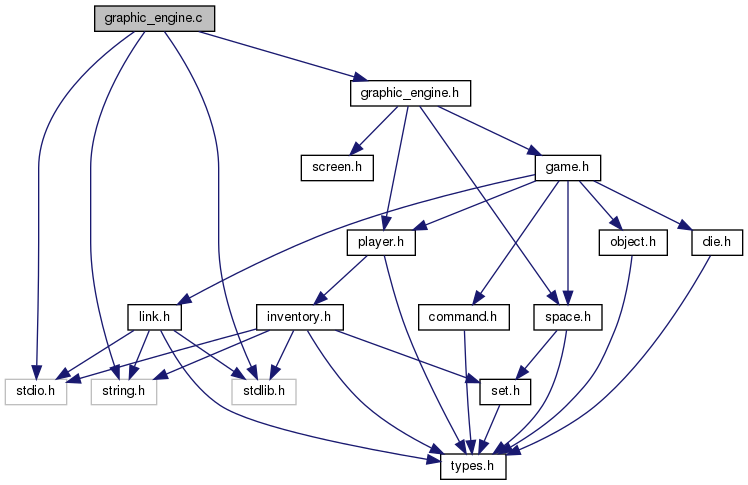
\includegraphics[width=350pt]{graphic__engine_8c__incl}
\end{center}
\end{figure}
\subsection*{Classes}
\begin{DoxyCompactItemize}
\item 
struct \hyperlink{struct__Graphic__engine}{\+\_\+\+Graphic\+\_\+engine}
\end{DoxyCompactItemize}
\subsection*{Functions}
\begin{DoxyCompactItemize}
\item 
\hyperlink{graphic__engine_8h_ae1bc5cdbfce93098f066274fdea49af1}{Graphic\+\_\+engine} $\ast$ \hyperlink{graphic__engine_8c_a8c3d9abe7282bee1d77d23ea80a4bdec}{graphic\+\_\+engine\+\_\+create} ()
\begin{DoxyCompactList}\small\item\em crea una interfaz grafica \end{DoxyCompactList}\item 
void \hyperlink{graphic__engine_8c_a5a5eac4ef2033c5ad71aa6895f362f79}{graphic\+\_\+engine\+\_\+destroy} (\hyperlink{graphic__engine_8h_ae1bc5cdbfce93098f066274fdea49af1}{Graphic\+\_\+engine} $\ast$ge)
\begin{DoxyCompactList}\small\item\em destruye una interfaz grafica \end{DoxyCompactList}\item 
void \hyperlink{graphic__engine_8c_a0e275aa477d5fa59e903da33a2a40a5d}{graphic\+\_\+engine\+\_\+paint\+\_\+game} (\hyperlink{graphic__engine_8h_ae1bc5cdbfce93098f066274fdea49af1}{Graphic\+\_\+engine} $\ast$ge, \hyperlink{game_8h_a57156d39c530aec3fba3a9dad8c2dc6a}{Game} $\ast$game)
\begin{DoxyCompactList}\small\item\em hace la interfaz grafica del juego \end{DoxyCompactList}\end{DoxyCompactItemize}


\subsection{Detailed Description}
En este fichero estaran las funciones relacionadas con la interfaz gráfica. 

\begin{DoxyAuthor}{Author}
Manuel Suarez, Saul Almazán, Álvaro Becerra, Rodrigo Lardiés 
\end{DoxyAuthor}
\begin{DoxyVersion}{Version}
2.\+0 
\end{DoxyVersion}
\begin{DoxyDate}{Date}
8/11/2018 
\end{DoxyDate}


\subsection{Function Documentation}
\mbox{\Hypertarget{graphic__engine_8c_a8c3d9abe7282bee1d77d23ea80a4bdec}\label{graphic__engine_8c_a8c3d9abe7282bee1d77d23ea80a4bdec}} 
\index{graphic\+\_\+engine.\+c@{graphic\+\_\+engine.\+c}!graphic\+\_\+engine\+\_\+create@{graphic\+\_\+engine\+\_\+create}}
\index{graphic\+\_\+engine\+\_\+create@{graphic\+\_\+engine\+\_\+create}!graphic\+\_\+engine.\+c@{graphic\+\_\+engine.\+c}}
\subsubsection{\texorpdfstring{graphic\+\_\+engine\+\_\+create()}{graphic\_engine\_create()}}
{\footnotesize\ttfamily \hyperlink{graphic__engine_8h_ae1bc5cdbfce93098f066274fdea49af1}{Graphic\+\_\+engine}$\ast$ graphic\+\_\+engine\+\_\+create (\begin{DoxyParamCaption}{ }\end{DoxyParamCaption})}



crea una interfaz grafica 

\begin{DoxyAuthor}{Author}
Manuel Suarez, Saul Almazán, Álvaro Becerra, Rodrigo Lardiés 
\end{DoxyAuthor}
\begin{DoxyDate}{Date}
8/11/2018 
\end{DoxyDate}
\begin{DoxyReturn}{Returns}
Graphic\+\_\+engine (la interfaz que hemos creado) 
\end{DoxyReturn}
\mbox{\Hypertarget{graphic__engine_8c_a5a5eac4ef2033c5ad71aa6895f362f79}\label{graphic__engine_8c_a5a5eac4ef2033c5ad71aa6895f362f79}} 
\index{graphic\+\_\+engine.\+c@{graphic\+\_\+engine.\+c}!graphic\+\_\+engine\+\_\+destroy@{graphic\+\_\+engine\+\_\+destroy}}
\index{graphic\+\_\+engine\+\_\+destroy@{graphic\+\_\+engine\+\_\+destroy}!graphic\+\_\+engine.\+c@{graphic\+\_\+engine.\+c}}
\subsubsection{\texorpdfstring{graphic\+\_\+engine\+\_\+destroy()}{graphic\_engine\_destroy()}}
{\footnotesize\ttfamily void graphic\+\_\+engine\+\_\+destroy (\begin{DoxyParamCaption}\item[{\hyperlink{graphic__engine_8h_ae1bc5cdbfce93098f066274fdea49af1}{Graphic\+\_\+engine} $\ast$}]{ge }\end{DoxyParamCaption})}



destruye una interfaz grafica 

\begin{DoxyAuthor}{Author}
Manuel Suarez, Saul Almazán, Álvaro Becerra, Rodrigo Lardiés 
\end{DoxyAuthor}
\begin{DoxyDate}{Date}
8/11/2018 
\end{DoxyDate}

\begin{DoxyParams}{Parameters}
{\em ge} & (la interfaz que se va a destruir) \\
\hline
\end{DoxyParams}
\begin{DoxyReturn}{Returns}
void (no devuelve nada) 
\end{DoxyReturn}
\mbox{\Hypertarget{graphic__engine_8c_a0e275aa477d5fa59e903da33a2a40a5d}\label{graphic__engine_8c_a0e275aa477d5fa59e903da33a2a40a5d}} 
\index{graphic\+\_\+engine.\+c@{graphic\+\_\+engine.\+c}!graphic\+\_\+engine\+\_\+paint\+\_\+game@{graphic\+\_\+engine\+\_\+paint\+\_\+game}}
\index{graphic\+\_\+engine\+\_\+paint\+\_\+game@{graphic\+\_\+engine\+\_\+paint\+\_\+game}!graphic\+\_\+engine.\+c@{graphic\+\_\+engine.\+c}}
\subsubsection{\texorpdfstring{graphic\+\_\+engine\+\_\+paint\+\_\+game()}{graphic\_engine\_paint\_game()}}
{\footnotesize\ttfamily void graphic\+\_\+engine\+\_\+paint\+\_\+game (\begin{DoxyParamCaption}\item[{\hyperlink{graphic__engine_8h_ae1bc5cdbfce93098f066274fdea49af1}{Graphic\+\_\+engine} $\ast$}]{ge,  }\item[{\hyperlink{game_8h_a57156d39c530aec3fba3a9dad8c2dc6a}{Game} $\ast$}]{game }\end{DoxyParamCaption})}



hace la interfaz grafica del juego 

\begin{DoxyAuthor}{Author}
Manuel Suarez, Saul Almazán, Álvaro Becerra, Rodrigo Lardiés 
\end{DoxyAuthor}
\begin{DoxyDate}{Date}
8/11/2018 
\end{DoxyDate}

\begin{DoxyParams}{Parameters}
{\em ge} & (la interfaz que se va a usar) \\
\hline
{\em game} & (El juego que se va a usar) \\
\hline
\end{DoxyParams}
\begin{DoxyReturn}{Returns}
void (no devuelve nada) 
\end{DoxyReturn}

\hypertarget{inventory_8c}{}\section{inventory.\+c File Reference}
\label{inventory_8c}\index{inventory.\+c@{inventory.\+c}}


En este fichero implementamos las funciones del inventario.  


{\ttfamily \#include \char`\"{}inventory.\+h\char`\"{}}\newline
Include dependency graph for inventory.\+c\+:\nopagebreak
\begin{figure}[H]
\begin{center}
\leavevmode
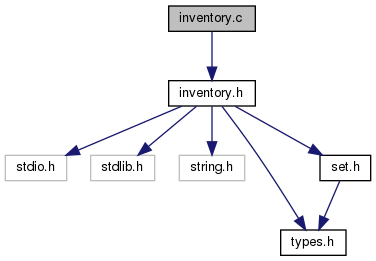
\includegraphics[width=350pt]{inventory_8c__incl}
\end{center}
\end{figure}
\subsection*{Classes}
\begin{DoxyCompactItemize}
\item 
struct \hyperlink{struct__Inventory}{\+\_\+\+Inventory}
\end{DoxyCompactItemize}
\subsection*{Functions}
\begin{DoxyCompactItemize}
\item 
\hyperlink{inventory_8h_a2253bf64ac4ce6a9c1d6f39c0b0d32a3}{Inventory} $\ast$ \hyperlink{inventory_8c_af7029a1a54b97f41fbd9f8437bf55ff9}{inventory\+\_\+create} (int tam)
\begin{DoxyCompactList}\small\item\em crea un inventario \end{DoxyCompactList}\item 
\hyperlink{types_8h_a32c27cc471df37f4fc818d65de0a56c4}{S\+T\+A\+T\+US} \hyperlink{inventory_8c_a654cebc804053355650fc71c49e79169}{inventory\+\_\+destroy} (\hyperlink{inventory_8h_a2253bf64ac4ce6a9c1d6f39c0b0d32a3}{Inventory} $\ast$bag)
\begin{DoxyCompactList}\small\item\em destruye un inventario \end{DoxyCompactList}\item 
\hyperlink{types_8h_a3e5b8192e7d9ffaf3542f1210aec18dd}{B\+O\+OL} \hyperlink{inventory_8c_a8284d16f802fe1225be5a34f0616dffd}{inventory\+\_\+is\+\_\+full} (\hyperlink{inventory_8h_a2253bf64ac4ce6a9c1d6f39c0b0d32a3}{Inventory} $\ast$bag)
\begin{DoxyCompactList}\small\item\em comprueba si el inventario esta lleno \end{DoxyCompactList}\item 
\hyperlink{types_8h_a3e5b8192e7d9ffaf3542f1210aec18dd}{B\+O\+OL} \hyperlink{inventory_8c_a2e42d41ecfb69141831596f72cd7d694}{inventory\+\_\+is\+\_\+empty} (\hyperlink{inventory_8h_a2253bf64ac4ce6a9c1d6f39c0b0d32a3}{Inventory} $\ast$bag)
\begin{DoxyCompactList}\small\item\em comprueba si el inventario esta vacio \end{DoxyCompactList}\item 
\hyperlink{types_8h_a3e5b8192e7d9ffaf3542f1210aec18dd}{B\+O\+OL} \hyperlink{inventory_8c_a15b54a6371860e214875899f790504b1}{inventory\+\_\+is\+\_\+object\+\_\+in} (\hyperlink{inventory_8h_a2253bf64ac4ce6a9c1d6f39c0b0d32a3}{Inventory} $\ast$bag, \hyperlink{types_8h_a845e604fb28f7e3d97549da3448149d3}{Id} id)
\begin{DoxyCompactList}\small\item\em comprueba si el objeto esta en el inventario \end{DoxyCompactList}\item 
\hyperlink{types_8h_a32c27cc471df37f4fc818d65de0a56c4}{S\+T\+A\+T\+US} \hyperlink{inventory_8c_a7bdb60da746304e8e80af87fb9c7ca92}{inventory\+\_\+add\+\_\+object} (\hyperlink{inventory_8h_a2253bf64ac4ce6a9c1d6f39c0b0d32a3}{Inventory} $\ast$bag, \hyperlink{types_8h_a845e604fb28f7e3d97549da3448149d3}{Id} id)
\begin{DoxyCompactList}\small\item\em añade un objeto del inventario \end{DoxyCompactList}\item 
\hyperlink{types_8h_a32c27cc471df37f4fc818d65de0a56c4}{S\+T\+A\+T\+US} \hyperlink{inventory_8c_a8b507ba4c2009e194c6338dd609186aa}{inventory\+\_\+delete\+\_\+object} (\hyperlink{inventory_8h_a2253bf64ac4ce6a9c1d6f39c0b0d32a3}{Inventory} $\ast$bag, \hyperlink{types_8h_a845e604fb28f7e3d97549da3448149d3}{Id} id)
\begin{DoxyCompactList}\small\item\em quita un objeto del inventario \end{DoxyCompactList}\item 
\hyperlink{set_8h_a6d3b7f7c92cbb4577ef3ef7ddbf93161}{Set} $\ast$ \hyperlink{inventory_8c_a60c25937b75342b2db4c18f3c21ace5f}{inventory\+\_\+get\+\_\+set} (\hyperlink{inventory_8h_a2253bf64ac4ce6a9c1d6f39c0b0d32a3}{Inventory} $\ast$bag)
\begin{DoxyCompactList}\small\item\em devuelve los objetos del inventario \end{DoxyCompactList}\item 
int \hyperlink{inventory_8c_ae13ea773456a53a0de513478940087a4}{inventory\+\_\+get\+\_\+size} (\hyperlink{inventory_8h_a2253bf64ac4ce6a9c1d6f39c0b0d32a3}{Inventory} $\ast$bag)
\begin{DoxyCompactList}\small\item\em devuelve el tamaño de un inventario \end{DoxyCompactList}\item 
\hyperlink{types_8h_a32c27cc471df37f4fc818d65de0a56c4}{S\+T\+A\+T\+US} \hyperlink{inventory_8c_aaf549db330cb81b574a0437ee8674e95}{inventory\+\_\+set\+\_\+set} (\hyperlink{inventory_8h_a2253bf64ac4ce6a9c1d6f39c0b0d32a3}{Inventory} $\ast$bag, \hyperlink{set_8h_a6d3b7f7c92cbb4577ef3ef7ddbf93161}{Set} $\ast$set)
\begin{DoxyCompactList}\small\item\em modifica los objetos de un inventario \end{DoxyCompactList}\item 
\hyperlink{types_8h_a32c27cc471df37f4fc818d65de0a56c4}{S\+T\+A\+T\+US} \hyperlink{inventory_8c_a4823fd1e3eb0d1d97d36600dafa0a78c}{inventory\+\_\+set\+\_\+size} (\hyperlink{inventory_8h_a2253bf64ac4ce6a9c1d6f39c0b0d32a3}{Inventory} $\ast$bag, int tam)
\begin{DoxyCompactList}\small\item\em cambia el tamaño de un inventario \end{DoxyCompactList}\item 
void \hyperlink{inventory_8c_a04e305db993339cf15c45aad1fa50144}{inventory\+\_\+print} (\hyperlink{inventory_8h_a2253bf64ac4ce6a9c1d6f39c0b0d32a3}{Inventory} $\ast$bag, F\+I\+LE $\ast$filename)
\begin{DoxyCompactList}\small\item\em imprime un inventario \end{DoxyCompactList}\end{DoxyCompactItemize}


\subsection{Detailed Description}
En este fichero implementamos las funciones del inventario. 

\begin{DoxyAuthor}{Author}
Manuel Suarez, Saul Almazán, Álvaro Becerra, Rodrigo Lardiés 
\end{DoxyAuthor}
\begin{DoxyVersion}{Version}
1.\+0 
\end{DoxyVersion}
\begin{DoxyDate}{Date}
10/11/2018 
\end{DoxyDate}


\subsection{Function Documentation}
\mbox{\Hypertarget{inventory_8c_a7bdb60da746304e8e80af87fb9c7ca92}\label{inventory_8c_a7bdb60da746304e8e80af87fb9c7ca92}} 
\index{inventory.\+c@{inventory.\+c}!inventory\+\_\+add\+\_\+object@{inventory\+\_\+add\+\_\+object}}
\index{inventory\+\_\+add\+\_\+object@{inventory\+\_\+add\+\_\+object}!inventory.\+c@{inventory.\+c}}
\subsubsection{\texorpdfstring{inventory\+\_\+add\+\_\+object()}{inventory\_add\_object()}}
{\footnotesize\ttfamily \hyperlink{types_8h_a32c27cc471df37f4fc818d65de0a56c4}{S\+T\+A\+T\+US} inventory\+\_\+add\+\_\+object (\begin{DoxyParamCaption}\item[{\hyperlink{inventory_8h_a2253bf64ac4ce6a9c1d6f39c0b0d32a3}{Inventory} $\ast$}]{bag,  }\item[{\hyperlink{types_8h_a845e604fb28f7e3d97549da3448149d3}{Id}}]{id }\end{DoxyParamCaption})}



añade un objeto del inventario 

\begin{DoxyAuthor}{Author}
Manuel Suarez, Saul Almazán, Álvaro Becerra, Rodrigo Lardiés 
\end{DoxyAuthor}
\begin{DoxyDate}{Date}
10/11/2018 
\end{DoxyDate}

\begin{DoxyParams}{Parameters}
{\em bag} & (inventario a modificar) \\
\hline
{\em id} & (Id del objeto) \\
\hline
\end{DoxyParams}
\begin{DoxyReturn}{Returns}
S\+T\+A\+T\+US (OK si se ha realizado correctamente o E\+R\+R\+OR de lo contrario) 
\end{DoxyReturn}
\mbox{\Hypertarget{inventory_8c_af7029a1a54b97f41fbd9f8437bf55ff9}\label{inventory_8c_af7029a1a54b97f41fbd9f8437bf55ff9}} 
\index{inventory.\+c@{inventory.\+c}!inventory\+\_\+create@{inventory\+\_\+create}}
\index{inventory\+\_\+create@{inventory\+\_\+create}!inventory.\+c@{inventory.\+c}}
\subsubsection{\texorpdfstring{inventory\+\_\+create()}{inventory\_create()}}
{\footnotesize\ttfamily \hyperlink{inventory_8h_a2253bf64ac4ce6a9c1d6f39c0b0d32a3}{Inventory}$\ast$ inventory\+\_\+create (\begin{DoxyParamCaption}\item[{int}]{tam }\end{DoxyParamCaption})}



crea un inventario 

\begin{DoxyAuthor}{Author}
Manuel Suarez, Saul Almazán, Álvaro Becerra, Rodrigo Lardiés 
\end{DoxyAuthor}
\begin{DoxyDate}{Date}
10/11/2018 
\end{DoxyDate}

\begin{DoxyParams}{Parameters}
{\em tam} & (tamaño del inventario) \\
\hline
\end{DoxyParams}
\begin{DoxyReturn}{Returns}
inventory$\ast$ (El inventario que crea) 
\end{DoxyReturn}
\mbox{\Hypertarget{inventory_8c_a8b507ba4c2009e194c6338dd609186aa}\label{inventory_8c_a8b507ba4c2009e194c6338dd609186aa}} 
\index{inventory.\+c@{inventory.\+c}!inventory\+\_\+delete\+\_\+object@{inventory\+\_\+delete\+\_\+object}}
\index{inventory\+\_\+delete\+\_\+object@{inventory\+\_\+delete\+\_\+object}!inventory.\+c@{inventory.\+c}}
\subsubsection{\texorpdfstring{inventory\+\_\+delete\+\_\+object()}{inventory\_delete\_object()}}
{\footnotesize\ttfamily \hyperlink{types_8h_a32c27cc471df37f4fc818d65de0a56c4}{S\+T\+A\+T\+US} inventory\+\_\+delete\+\_\+object (\begin{DoxyParamCaption}\item[{\hyperlink{inventory_8h_a2253bf64ac4ce6a9c1d6f39c0b0d32a3}{Inventory} $\ast$}]{bag,  }\item[{\hyperlink{types_8h_a845e604fb28f7e3d97549da3448149d3}{Id}}]{id }\end{DoxyParamCaption})}



quita un objeto del inventario 

\begin{DoxyAuthor}{Author}
Manuel Suarez, Saul Almazán, Álvaro Becerra, Rodrigo Lardiés 
\end{DoxyAuthor}
\begin{DoxyDate}{Date}
10/11/2018 
\end{DoxyDate}

\begin{DoxyParams}{Parameters}
{\em bag} & (inventario a modificar) \\
\hline
{\em id} & (Id del objeto) \\
\hline
\end{DoxyParams}
\begin{DoxyReturn}{Returns}
S\+T\+A\+T\+US (OK si se ha realizado correctamente o E\+R\+R\+OR de lo contrario) 
\end{DoxyReturn}
\mbox{\Hypertarget{inventory_8c_a654cebc804053355650fc71c49e79169}\label{inventory_8c_a654cebc804053355650fc71c49e79169}} 
\index{inventory.\+c@{inventory.\+c}!inventory\+\_\+destroy@{inventory\+\_\+destroy}}
\index{inventory\+\_\+destroy@{inventory\+\_\+destroy}!inventory.\+c@{inventory.\+c}}
\subsubsection{\texorpdfstring{inventory\+\_\+destroy()}{inventory\_destroy()}}
{\footnotesize\ttfamily \hyperlink{types_8h_a32c27cc471df37f4fc818d65de0a56c4}{S\+T\+A\+T\+US} inventory\+\_\+destroy (\begin{DoxyParamCaption}\item[{\hyperlink{inventory_8h_a2253bf64ac4ce6a9c1d6f39c0b0d32a3}{Inventory} $\ast$}]{bag }\end{DoxyParamCaption})}



destruye un inventario 

\begin{DoxyAuthor}{Author}
Manuel Suarez, Saul Almazán, Álvaro Becerra, Rodrigo Lardiés 
\end{DoxyAuthor}
\begin{DoxyDate}{Date}
10/11/2018 
\end{DoxyDate}

\begin{DoxyParams}{Parameters}
{\em bag} & (inventario a destruir) \\
\hline
\end{DoxyParams}
\begin{DoxyReturn}{Returns}
S\+T\+A\+T\+US (OK si se ha realizado correctamente o E\+R\+R\+OR de lo contrario) 
\end{DoxyReturn}
\mbox{\Hypertarget{inventory_8c_a60c25937b75342b2db4c18f3c21ace5f}\label{inventory_8c_a60c25937b75342b2db4c18f3c21ace5f}} 
\index{inventory.\+c@{inventory.\+c}!inventory\+\_\+get\+\_\+set@{inventory\+\_\+get\+\_\+set}}
\index{inventory\+\_\+get\+\_\+set@{inventory\+\_\+get\+\_\+set}!inventory.\+c@{inventory.\+c}}
\subsubsection{\texorpdfstring{inventory\+\_\+get\+\_\+set()}{inventory\_get\_set()}}
{\footnotesize\ttfamily \hyperlink{set_8h_a6d3b7f7c92cbb4577ef3ef7ddbf93161}{Set}$\ast$ inventory\+\_\+get\+\_\+set (\begin{DoxyParamCaption}\item[{\hyperlink{inventory_8h_a2253bf64ac4ce6a9c1d6f39c0b0d32a3}{Inventory} $\ast$}]{bag }\end{DoxyParamCaption})}



devuelve los objetos del inventario 

\begin{DoxyAuthor}{Author}
Manuel Suarez, Saul Almazán, Álvaro Becerra, Rodrigo Lardiés 
\end{DoxyAuthor}
\begin{DoxyDate}{Date}
10/11/2018 
\end{DoxyDate}

\begin{DoxyParams}{Parameters}
{\em bag} & (inventario a destruir) \\
\hline
\end{DoxyParams}
\begin{DoxyReturn}{Returns}
Set (Objetos del inventario) 
\end{DoxyReturn}
\mbox{\Hypertarget{inventory_8c_ae13ea773456a53a0de513478940087a4}\label{inventory_8c_ae13ea773456a53a0de513478940087a4}} 
\index{inventory.\+c@{inventory.\+c}!inventory\+\_\+get\+\_\+size@{inventory\+\_\+get\+\_\+size}}
\index{inventory\+\_\+get\+\_\+size@{inventory\+\_\+get\+\_\+size}!inventory.\+c@{inventory.\+c}}
\subsubsection{\texorpdfstring{inventory\+\_\+get\+\_\+size()}{inventory\_get\_size()}}
{\footnotesize\ttfamily int inventory\+\_\+get\+\_\+size (\begin{DoxyParamCaption}\item[{\hyperlink{inventory_8h_a2253bf64ac4ce6a9c1d6f39c0b0d32a3}{Inventory} $\ast$}]{bag }\end{DoxyParamCaption})}



devuelve el tamaño de un inventario 

\begin{DoxyAuthor}{Author}
Manuel Suarez, Saul Almazán, Álvaro Becerra, Rodrigo Lardiés 
\end{DoxyAuthor}
\begin{DoxyDate}{Date}
10/11/2018 
\end{DoxyDate}

\begin{DoxyParams}{Parameters}
{\em bag} & (inventario a usar) \\
\hline
\end{DoxyParams}
\begin{DoxyReturn}{Returns}
int (Tamaño del inventario) 
\end{DoxyReturn}
\mbox{\Hypertarget{inventory_8c_a2e42d41ecfb69141831596f72cd7d694}\label{inventory_8c_a2e42d41ecfb69141831596f72cd7d694}} 
\index{inventory.\+c@{inventory.\+c}!inventory\+\_\+is\+\_\+empty@{inventory\+\_\+is\+\_\+empty}}
\index{inventory\+\_\+is\+\_\+empty@{inventory\+\_\+is\+\_\+empty}!inventory.\+c@{inventory.\+c}}
\subsubsection{\texorpdfstring{inventory\+\_\+is\+\_\+empty()}{inventory\_is\_empty()}}
{\footnotesize\ttfamily \hyperlink{types_8h_a3e5b8192e7d9ffaf3542f1210aec18dd}{B\+O\+OL} inventory\+\_\+is\+\_\+empty (\begin{DoxyParamCaption}\item[{\hyperlink{inventory_8h_a2253bf64ac4ce6a9c1d6f39c0b0d32a3}{Inventory} $\ast$}]{bag }\end{DoxyParamCaption})}



comprueba si el inventario esta vacio 

\begin{DoxyAuthor}{Author}
Manuel Suarez, Saul Almazán, Álvaro Becerra, Rodrigo Lardiés 
\end{DoxyAuthor}
\begin{DoxyDate}{Date}
10/11/2018 
\end{DoxyDate}

\begin{DoxyParams}{Parameters}
{\em bag} & (inventario a usar) \\
\hline
\end{DoxyParams}
\begin{DoxyReturn}{Returns}
B\+O\+OL (T\+R\+UE si esta vacio o F\+A\+L\+SE de lo contrario) 
\end{DoxyReturn}
\mbox{\Hypertarget{inventory_8c_a8284d16f802fe1225be5a34f0616dffd}\label{inventory_8c_a8284d16f802fe1225be5a34f0616dffd}} 
\index{inventory.\+c@{inventory.\+c}!inventory\+\_\+is\+\_\+full@{inventory\+\_\+is\+\_\+full}}
\index{inventory\+\_\+is\+\_\+full@{inventory\+\_\+is\+\_\+full}!inventory.\+c@{inventory.\+c}}
\subsubsection{\texorpdfstring{inventory\+\_\+is\+\_\+full()}{inventory\_is\_full()}}
{\footnotesize\ttfamily \hyperlink{types_8h_a3e5b8192e7d9ffaf3542f1210aec18dd}{B\+O\+OL} inventory\+\_\+is\+\_\+full (\begin{DoxyParamCaption}\item[{\hyperlink{inventory_8h_a2253bf64ac4ce6a9c1d6f39c0b0d32a3}{Inventory} $\ast$}]{bag }\end{DoxyParamCaption})}



comprueba si el inventario esta lleno 

\begin{DoxyAuthor}{Author}
Manuel Suarez, Saul Almazán, Álvaro Becerra, Rodrigo Lardiés 
\end{DoxyAuthor}
\begin{DoxyDate}{Date}
10/11/2018 
\end{DoxyDate}

\begin{DoxyParams}{Parameters}
{\em bag} & (inventario a usar) \\
\hline
\end{DoxyParams}
\begin{DoxyReturn}{Returns}
B\+O\+OL (T\+R\+UE si esta lleno o F\+A\+L\+SE de lo contrario) 
\end{DoxyReturn}
\mbox{\Hypertarget{inventory_8c_a15b54a6371860e214875899f790504b1}\label{inventory_8c_a15b54a6371860e214875899f790504b1}} 
\index{inventory.\+c@{inventory.\+c}!inventory\+\_\+is\+\_\+object\+\_\+in@{inventory\+\_\+is\+\_\+object\+\_\+in}}
\index{inventory\+\_\+is\+\_\+object\+\_\+in@{inventory\+\_\+is\+\_\+object\+\_\+in}!inventory.\+c@{inventory.\+c}}
\subsubsection{\texorpdfstring{inventory\+\_\+is\+\_\+object\+\_\+in()}{inventory\_is\_object\_in()}}
{\footnotesize\ttfamily \hyperlink{types_8h_a3e5b8192e7d9ffaf3542f1210aec18dd}{B\+O\+OL} inventory\+\_\+is\+\_\+object\+\_\+in (\begin{DoxyParamCaption}\item[{\hyperlink{inventory_8h_a2253bf64ac4ce6a9c1d6f39c0b0d32a3}{Inventory} $\ast$}]{bag,  }\item[{\hyperlink{types_8h_a845e604fb28f7e3d97549da3448149d3}{Id}}]{id }\end{DoxyParamCaption})}



comprueba si el objeto esta en el inventario 

\begin{DoxyAuthor}{Author}
Manuel Suarez, Saul Almazán, Álvaro Becerra, Rodrigo Lardiés 
\end{DoxyAuthor}
\begin{DoxyDate}{Date}
10/11/2018 
\end{DoxyDate}

\begin{DoxyParams}{Parameters}
{\em bag} & (inventario a usar) \\
\hline
{\em id} & (Id del objeto) \\
\hline
\end{DoxyParams}
\begin{DoxyReturn}{Returns}
B\+O\+OL (T\+R\+UE si esta en el inventario o F\+A\+L\+SE de lo contrario) 
\end{DoxyReturn}
\mbox{\Hypertarget{inventory_8c_a04e305db993339cf15c45aad1fa50144}\label{inventory_8c_a04e305db993339cf15c45aad1fa50144}} 
\index{inventory.\+c@{inventory.\+c}!inventory\+\_\+print@{inventory\+\_\+print}}
\index{inventory\+\_\+print@{inventory\+\_\+print}!inventory.\+c@{inventory.\+c}}
\subsubsection{\texorpdfstring{inventory\+\_\+print()}{inventory\_print()}}
{\footnotesize\ttfamily void inventory\+\_\+print (\begin{DoxyParamCaption}\item[{\hyperlink{inventory_8h_a2253bf64ac4ce6a9c1d6f39c0b0d32a3}{Inventory} $\ast$}]{bag,  }\item[{F\+I\+LE $\ast$}]{filename }\end{DoxyParamCaption})}



imprime un inventario 

\begin{DoxyAuthor}{Author}
Manuel Suarez, Saul Almazán, Álvaro Becerra, Rodrigo Lardiés 
\end{DoxyAuthor}
\begin{DoxyDate}{Date}
10/11/2018 
\end{DoxyDate}

\begin{DoxyParams}{Parameters}
{\em bag} & (inventario a imprimir) \\
\hline
{\em filename} & (Donde se imprime) \\
\hline
\end{DoxyParams}
\begin{DoxyReturn}{Returns}
void (No devuelve nada) 
\end{DoxyReturn}
\mbox{\Hypertarget{inventory_8c_aaf549db330cb81b574a0437ee8674e95}\label{inventory_8c_aaf549db330cb81b574a0437ee8674e95}} 
\index{inventory.\+c@{inventory.\+c}!inventory\+\_\+set\+\_\+set@{inventory\+\_\+set\+\_\+set}}
\index{inventory\+\_\+set\+\_\+set@{inventory\+\_\+set\+\_\+set}!inventory.\+c@{inventory.\+c}}
\subsubsection{\texorpdfstring{inventory\+\_\+set\+\_\+set()}{inventory\_set\_set()}}
{\footnotesize\ttfamily \hyperlink{types_8h_a32c27cc471df37f4fc818d65de0a56c4}{S\+T\+A\+T\+US} inventory\+\_\+set\+\_\+set (\begin{DoxyParamCaption}\item[{\hyperlink{inventory_8h_a2253bf64ac4ce6a9c1d6f39c0b0d32a3}{Inventory} $\ast$}]{bag,  }\item[{\hyperlink{set_8h_a6d3b7f7c92cbb4577ef3ef7ddbf93161}{Set} $\ast$}]{set }\end{DoxyParamCaption})}



modifica los objetos de un inventario 

\begin{DoxyAuthor}{Author}
Manuel Suarez, Saul Almazán, Álvaro Becerra, Rodrigo Lardiés 
\end{DoxyAuthor}
\begin{DoxyDate}{Date}
10/11/2018 
\end{DoxyDate}

\begin{DoxyParams}{Parameters}
{\em bag} & (inventario a modificar) \\
\hline
{\em set} & (Objetos nuevos del inventario) \\
\hline
\end{DoxyParams}
\begin{DoxyReturn}{Returns}
S\+T\+A\+T\+US (OK si se ha realizado correctamente o E\+R\+R\+OR de lo contrario) 
\end{DoxyReturn}
\mbox{\Hypertarget{inventory_8c_a4823fd1e3eb0d1d97d36600dafa0a78c}\label{inventory_8c_a4823fd1e3eb0d1d97d36600dafa0a78c}} 
\index{inventory.\+c@{inventory.\+c}!inventory\+\_\+set\+\_\+size@{inventory\+\_\+set\+\_\+size}}
\index{inventory\+\_\+set\+\_\+size@{inventory\+\_\+set\+\_\+size}!inventory.\+c@{inventory.\+c}}
\subsubsection{\texorpdfstring{inventory\+\_\+set\+\_\+size()}{inventory\_set\_size()}}
{\footnotesize\ttfamily \hyperlink{types_8h_a32c27cc471df37f4fc818d65de0a56c4}{S\+T\+A\+T\+US} inventory\+\_\+set\+\_\+size (\begin{DoxyParamCaption}\item[{\hyperlink{inventory_8h_a2253bf64ac4ce6a9c1d6f39c0b0d32a3}{Inventory} $\ast$}]{bag,  }\item[{int}]{tam }\end{DoxyParamCaption})}



cambia el tamaño de un inventario 

\begin{DoxyAuthor}{Author}
Manuel Suarez, Saul Almazán, Álvaro Becerra, Rodrigo Lardiés 
\end{DoxyAuthor}
\begin{DoxyDate}{Date}
10/11/2018 
\end{DoxyDate}

\begin{DoxyParams}{Parameters}
{\em bag} & (inventario que se va a cambiar) \\
\hline
{\em tam} & (tamaño nuevo del inventario) \\
\hline
\end{DoxyParams}
\begin{DoxyReturn}{Returns}
S\+T\+A\+T\+US (OK si se ha realizado correctamente o E\+R\+R\+OR de lo contrario) 
\end{DoxyReturn}

\hypertarget{inventory__test_8c}{}\section{inventory\+\_\+test.\+c File Reference}
\label{inventory__test_8c}\index{inventory\+\_\+test.\+c@{inventory\+\_\+test.\+c}}


En este fichero probamos las funciones del inventario.  


{\ttfamily \#include $<$stdio.\+h$>$}\newline
{\ttfamily \#include $<$stdlib.\+h$>$}\newline
{\ttfamily \#include $<$string.\+h$>$}\newline
{\ttfamily \#include \char`\"{}inventory.\+h\char`\"{}}\newline
Include dependency graph for inventory\+\_\+test.\+c\+:\nopagebreak
\begin{figure}[H]
\begin{center}
\leavevmode
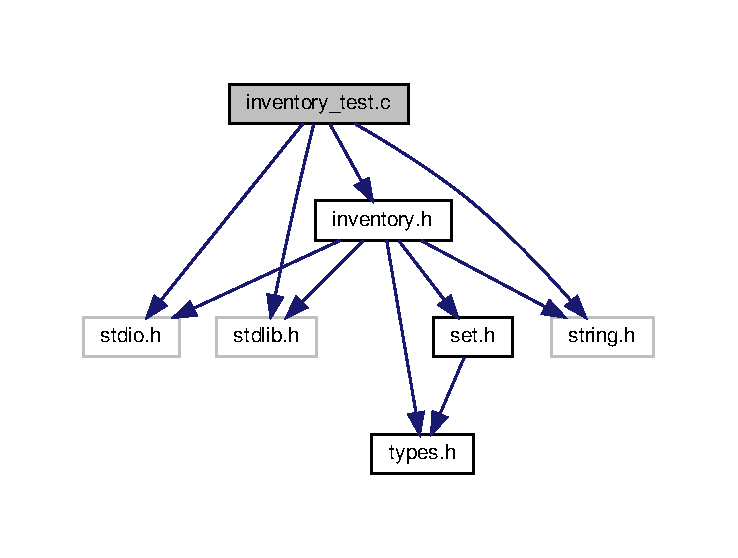
\includegraphics[width=350pt]{inventory__test_8c__incl}
\end{center}
\end{figure}
\subsection*{Functions}
\begin{DoxyCompactItemize}
\item 
int \hyperlink{inventory__test_8c_a0ddf1224851353fc92bfbff6f499fa97}{main} (int argc, char $\ast$argv\mbox{[}$\,$\mbox{]})
\begin{DoxyCompactList}\small\item\em funcion principal de prueba del inventario \end{DoxyCompactList}\end{DoxyCompactItemize}


\subsection{Detailed Description}
En este fichero probamos las funciones del inventario. 

\begin{DoxyAuthor}{Author}
Manuel Suarez, Saul Almazán, Álvaro Becerra, Rodrigo Lardiés 
\end{DoxyAuthor}
\begin{DoxyVersion}{Version}
1.\+0 
\end{DoxyVersion}
\begin{DoxyDate}{Date}
10/11/2018 
\end{DoxyDate}


\subsection{Function Documentation}
\mbox{\Hypertarget{inventory__test_8c_a0ddf1224851353fc92bfbff6f499fa97}\label{inventory__test_8c_a0ddf1224851353fc92bfbff6f499fa97}} 
\index{inventory\+\_\+test.\+c@{inventory\+\_\+test.\+c}!main@{main}}
\index{main@{main}!inventory\+\_\+test.\+c@{inventory\+\_\+test.\+c}}
\subsubsection{\texorpdfstring{main()}{main()}}
{\footnotesize\ttfamily int main (\begin{DoxyParamCaption}\item[{int}]{argc,  }\item[{char $\ast$}]{argv\mbox{[}$\,$\mbox{]} }\end{DoxyParamCaption})}



funcion principal de prueba del inventario 

\begin{DoxyAuthor}{Author}
Manuel Suarez, Saul Almazán, Álvaro Becerra, Rodrigo Lardiés 
\end{DoxyAuthor}
\begin{DoxyDate}{Date}
10/11/2018 
\end{DoxyDate}

\begin{DoxyParams}{Parameters}
{\em argc} & (numero de argumentos) \\
\hline
{\em argv\mbox{[}$\,$\mbox{]}} & (argumentos) \\
\hline
\end{DoxyParams}
\begin{DoxyReturn}{Returns}
int 
\end{DoxyReturn}

\hypertarget{link_8c}{}\section{link.\+c File Reference}
\label{link_8c}\index{link.\+c@{link.\+c}}


En este fichero implementamos las funciones de link.  


{\ttfamily \#include $<$stdio.\+h$>$}\newline
{\ttfamily \#include $<$stdlib.\+h$>$}\newline
{\ttfamily \#include \char`\"{}link.\+h\char`\"{}}\newline
Include dependency graph for link.\+c\+:\nopagebreak
\begin{figure}[H]
\begin{center}
\leavevmode
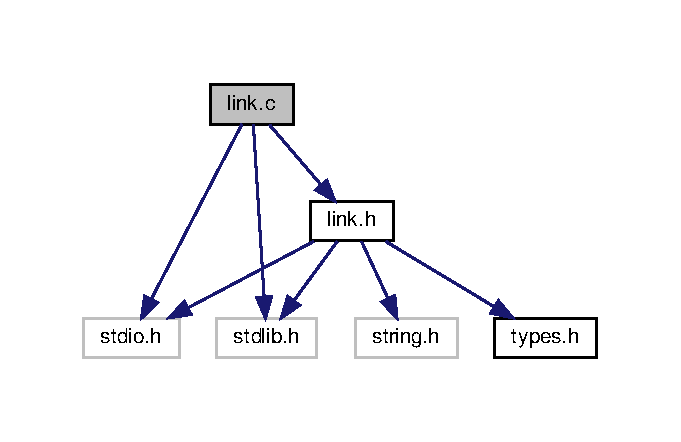
\includegraphics[width=327pt]{link_8c__incl}
\end{center}
\end{figure}
\subsection*{Classes}
\begin{DoxyCompactItemize}
\item 
struct \hyperlink{struct__Link}{\+\_\+\+Link}
\end{DoxyCompactItemize}
\subsection*{Functions}
\begin{DoxyCompactItemize}
\item 
\hyperlink{link_8h_ae3b299941e67be6971bfd64a25505eff}{Link} $\ast$ \hyperlink{link_8c_aaf21d03943afcbed370ca720f972482c}{link\+\_\+create} ()
\begin{DoxyCompactList}\small\item\em crea un link \end{DoxyCompactList}\item 
void \hyperlink{link_8c_a117e4e5a82b23b805052d1eace34d068}{link\+\_\+destroy} (\hyperlink{link_8h_ae3b299941e67be6971bfd64a25505eff}{Link} $\ast$link)
\begin{DoxyCompactList}\small\item\em destruye y libera la memoria de un link \end{DoxyCompactList}\item 
\hyperlink{types_8h_a845e604fb28f7e3d97549da3448149d3}{Id} \hyperlink{link_8c_a2bbd320f995a72b2ea7ea639b1c81892}{link\+\_\+get\+\_\+id} (\hyperlink{link_8h_ae3b299941e67be6971bfd64a25505eff}{Link} $\ast$link)
\begin{DoxyCompactList}\small\item\em devuelve el Id de un link \end{DoxyCompactList}\item 
char $\ast$ \hyperlink{link_8c_a9747ee8201a323e112e67bdeacbc90d8}{link\+\_\+get\+\_\+name} (\hyperlink{link_8h_ae3b299941e67be6971bfd64a25505eff}{Link} $\ast$link)
\begin{DoxyCompactList}\small\item\em devuelve el Id de un link \end{DoxyCompactList}\item 
\hyperlink{types_8h_a845e604fb28f7e3d97549da3448149d3}{Id} \hyperlink{link_8c_a8b02c6629b52f2be8fa22c8f3f7466fe}{link\+\_\+get\+\_\+conection\+\_\+1} (\hyperlink{link_8h_ae3b299941e67be6971bfd64a25505eff}{Link} $\ast$link)
\begin{DoxyCompactList}\small\item\em el Id de la conexion 1 del link \end{DoxyCompactList}\item 
\hyperlink{types_8h_a845e604fb28f7e3d97549da3448149d3}{Id} \hyperlink{link_8c_ae49357746643a5e0786c6c1c843f0351}{link\+\_\+get\+\_\+conection\+\_\+2} (\hyperlink{link_8h_ae3b299941e67be6971bfd64a25505eff}{Link} $\ast$link)
\begin{DoxyCompactList}\small\item\em el Id de la conexion 2 del link \end{DoxyCompactList}\item 
\hyperlink{types_8h_a3e5b8192e7d9ffaf3542f1210aec18dd}{B\+O\+OL} \hyperlink{link_8c_af50c9578ed458d4ef4f4c85bdb60b3e1}{link\+\_\+get\+\_\+status} (\hyperlink{link_8h_ae3b299941e67be6971bfd64a25505eff}{Link} $\ast$link)
\begin{DoxyCompactList}\small\item\em comprueba si la conexion esta abierta o cerrada \end{DoxyCompactList}\item 
\hyperlink{types_8h_a32c27cc471df37f4fc818d65de0a56c4}{S\+T\+A\+T\+US} \hyperlink{link_8c_a3fd49fb1a3f19be4fc800ff07820cafb}{link\+\_\+set\+\_\+id} (\hyperlink{link_8h_ae3b299941e67be6971bfd64a25505eff}{Link} $\ast$link, \hyperlink{types_8h_a845e604fb28f7e3d97549da3448149d3}{Id} id)
\begin{DoxyCompactList}\small\item\em modifica el Id de un link \end{DoxyCompactList}\item 
\hyperlink{types_8h_a32c27cc471df37f4fc818d65de0a56c4}{S\+T\+A\+T\+US} \hyperlink{link_8c_a6c7a3bd7a856288c377edbcd045912e6}{link\+\_\+set\+\_\+name} (\hyperlink{link_8h_ae3b299941e67be6971bfd64a25505eff}{Link} $\ast$link, char $\ast$name)
\begin{DoxyCompactList}\small\item\em modifica el nombre de un link \end{DoxyCompactList}\item 
\hyperlink{types_8h_a32c27cc471df37f4fc818d65de0a56c4}{S\+T\+A\+T\+US} \hyperlink{link_8c_a93bfde2dd6d354dfca04cf0643317433}{link\+\_\+set\+\_\+conection} (\hyperlink{link_8h_ae3b299941e67be6971bfd64a25505eff}{Link} $\ast$link, \hyperlink{types_8h_a845e604fb28f7e3d97549da3448149d3}{Id} id1, \hyperlink{types_8h_a845e604fb28f7e3d97549da3448149d3}{Id} id2)
\begin{DoxyCompactList}\small\item\em modifica ela conexion de un link \end{DoxyCompactList}\item 
\hyperlink{types_8h_a32c27cc471df37f4fc818d65de0a56c4}{S\+T\+A\+T\+US} \hyperlink{link_8c_a9cd26b9d2d38b901380885e8ea7edec4}{link\+\_\+set\+\_\+status} (\hyperlink{link_8h_ae3b299941e67be6971bfd64a25505eff}{Link} $\ast$link, \hyperlink{types_8h_a3e5b8192e7d9ffaf3542f1210aec18dd}{B\+O\+OL} bool)
\begin{DoxyCompactList}\small\item\em modifica el estado de un link \end{DoxyCompactList}\item 
int \hyperlink{link_8c_ab5c45f8c1edc80d2f2dd73f5539d1951}{link\+\_\+print} (\hyperlink{link_8h_ae3b299941e67be6971bfd64a25505eff}{Link} $\ast$link)
\begin{DoxyCompactList}\small\item\em imprime un link \end{DoxyCompactList}\end{DoxyCompactItemize}


\subsection{Detailed Description}
En este fichero implementamos las funciones de link. 

\begin{DoxyAuthor}{Author}
Manuel Suarez, Saul Almazán, Álvaro Becerra, Rodrigo Lardiés 
\end{DoxyAuthor}
\begin{DoxyVersion}{Version}
1.\+0 
\end{DoxyVersion}
\begin{DoxyDate}{Date}
15/11/2018 
\end{DoxyDate}


\subsection{Function Documentation}
\mbox{\Hypertarget{link_8c_aaf21d03943afcbed370ca720f972482c}\label{link_8c_aaf21d03943afcbed370ca720f972482c}} 
\index{link.\+c@{link.\+c}!link\+\_\+create@{link\+\_\+create}}
\index{link\+\_\+create@{link\+\_\+create}!link.\+c@{link.\+c}}
\subsubsection{\texorpdfstring{link\+\_\+create()}{link\_create()}}
{\footnotesize\ttfamily \hyperlink{link_8h_ae3b299941e67be6971bfd64a25505eff}{Link}$\ast$ link\+\_\+create (\begin{DoxyParamCaption}{ }\end{DoxyParamCaption})}



crea un link 

\begin{DoxyAuthor}{Author}
Manuel Suarez, Saul Almazán, Álvaro Becerra, Rodrigo Lardiés 
\end{DoxyAuthor}
\begin{DoxyDate}{Date}
15/11/2018 
\end{DoxyDate}
\begin{DoxyReturn}{Returns}
Link (El link que crea) 
\end{DoxyReturn}
\mbox{\Hypertarget{link_8c_a117e4e5a82b23b805052d1eace34d068}\label{link_8c_a117e4e5a82b23b805052d1eace34d068}} 
\index{link.\+c@{link.\+c}!link\+\_\+destroy@{link\+\_\+destroy}}
\index{link\+\_\+destroy@{link\+\_\+destroy}!link.\+c@{link.\+c}}
\subsubsection{\texorpdfstring{link\+\_\+destroy()}{link\_destroy()}}
{\footnotesize\ttfamily void link\+\_\+destroy (\begin{DoxyParamCaption}\item[{\hyperlink{link_8h_ae3b299941e67be6971bfd64a25505eff}{Link} $\ast$}]{link }\end{DoxyParamCaption})}



destruye y libera la memoria de un link 

\begin{DoxyAuthor}{Author}
Manuel Suarez, Saul Almazán, Álvaro Becerra, Rodrigo Lardiés 
\end{DoxyAuthor}
\begin{DoxyDate}{Date}
15/11/2018 
\end{DoxyDate}

\begin{DoxyParams}{Parameters}
{\em link} & (link a destruir) \\
\hline
\end{DoxyParams}
\begin{DoxyReturn}{Returns}
void (No devuelve nada) 
\end{DoxyReturn}
\mbox{\Hypertarget{link_8c_a8b02c6629b52f2be8fa22c8f3f7466fe}\label{link_8c_a8b02c6629b52f2be8fa22c8f3f7466fe}} 
\index{link.\+c@{link.\+c}!link\+\_\+get\+\_\+conection\+\_\+1@{link\+\_\+get\+\_\+conection\+\_\+1}}
\index{link\+\_\+get\+\_\+conection\+\_\+1@{link\+\_\+get\+\_\+conection\+\_\+1}!link.\+c@{link.\+c}}
\subsubsection{\texorpdfstring{link\+\_\+get\+\_\+conection\+\_\+1()}{link\_get\_conection\_1()}}
{\footnotesize\ttfamily \hyperlink{types_8h_a845e604fb28f7e3d97549da3448149d3}{Id} link\+\_\+get\+\_\+conection\+\_\+1 (\begin{DoxyParamCaption}\item[{\hyperlink{link_8h_ae3b299941e67be6971bfd64a25505eff}{Link} $\ast$}]{link }\end{DoxyParamCaption})}



el Id de la conexion 1 del link 

\begin{DoxyAuthor}{Author}
Manuel Suarez, Saul Almazán, Álvaro Becerra, Rodrigo Lardiés 
\end{DoxyAuthor}
\begin{DoxyDate}{Date}
15/11/2018 
\end{DoxyDate}

\begin{DoxyParams}{Parameters}
{\em link} & (link a usar) \\
\hline
\end{DoxyParams}
\begin{DoxyReturn}{Returns}
Id (Id de la conexion) 
\end{DoxyReturn}
\mbox{\Hypertarget{link_8c_ae49357746643a5e0786c6c1c843f0351}\label{link_8c_ae49357746643a5e0786c6c1c843f0351}} 
\index{link.\+c@{link.\+c}!link\+\_\+get\+\_\+conection\+\_\+2@{link\+\_\+get\+\_\+conection\+\_\+2}}
\index{link\+\_\+get\+\_\+conection\+\_\+2@{link\+\_\+get\+\_\+conection\+\_\+2}!link.\+c@{link.\+c}}
\subsubsection{\texorpdfstring{link\+\_\+get\+\_\+conection\+\_\+2()}{link\_get\_conection\_2()}}
{\footnotesize\ttfamily \hyperlink{types_8h_a845e604fb28f7e3d97549da3448149d3}{Id} link\+\_\+get\+\_\+conection\+\_\+2 (\begin{DoxyParamCaption}\item[{\hyperlink{link_8h_ae3b299941e67be6971bfd64a25505eff}{Link} $\ast$}]{link }\end{DoxyParamCaption})}



el Id de la conexion 2 del link 

\begin{DoxyAuthor}{Author}
Manuel Suarez, Saul Almazán, Álvaro Becerra, Rodrigo Lardiés 
\end{DoxyAuthor}
\begin{DoxyDate}{Date}
15/11/2018 
\end{DoxyDate}

\begin{DoxyParams}{Parameters}
{\em link} & (link a usar) \\
\hline
\end{DoxyParams}
\begin{DoxyReturn}{Returns}
Id (Id de la conexion) 
\end{DoxyReturn}
\mbox{\Hypertarget{link_8c_a2bbd320f995a72b2ea7ea639b1c81892}\label{link_8c_a2bbd320f995a72b2ea7ea639b1c81892}} 
\index{link.\+c@{link.\+c}!link\+\_\+get\+\_\+id@{link\+\_\+get\+\_\+id}}
\index{link\+\_\+get\+\_\+id@{link\+\_\+get\+\_\+id}!link.\+c@{link.\+c}}
\subsubsection{\texorpdfstring{link\+\_\+get\+\_\+id()}{link\_get\_id()}}
{\footnotesize\ttfamily \hyperlink{types_8h_a845e604fb28f7e3d97549da3448149d3}{Id} link\+\_\+get\+\_\+id (\begin{DoxyParamCaption}\item[{\hyperlink{link_8h_ae3b299941e67be6971bfd64a25505eff}{Link} $\ast$}]{link }\end{DoxyParamCaption})}



devuelve el Id de un link 

\begin{DoxyAuthor}{Author}
Manuel Suarez, Saul Almazán, Álvaro Becerra, Rodrigo Lardiés 
\end{DoxyAuthor}
\begin{DoxyDate}{Date}
15/11/2018 
\end{DoxyDate}

\begin{DoxyParams}{Parameters}
{\em link} & (link a usar) \\
\hline
\end{DoxyParams}
\begin{DoxyReturn}{Returns}
Id (Id del link) 
\end{DoxyReturn}
\mbox{\Hypertarget{link_8c_a9747ee8201a323e112e67bdeacbc90d8}\label{link_8c_a9747ee8201a323e112e67bdeacbc90d8}} 
\index{link.\+c@{link.\+c}!link\+\_\+get\+\_\+name@{link\+\_\+get\+\_\+name}}
\index{link\+\_\+get\+\_\+name@{link\+\_\+get\+\_\+name}!link.\+c@{link.\+c}}
\subsubsection{\texorpdfstring{link\+\_\+get\+\_\+name()}{link\_get\_name()}}
{\footnotesize\ttfamily char$\ast$ link\+\_\+get\+\_\+name (\begin{DoxyParamCaption}\item[{\hyperlink{link_8h_ae3b299941e67be6971bfd64a25505eff}{Link} $\ast$}]{link }\end{DoxyParamCaption})}



devuelve el Id de un link 

\begin{DoxyAuthor}{Author}
Manuel Suarez, Saul Almazán, Álvaro Becerra, Rodrigo Lardiés 
\end{DoxyAuthor}
\begin{DoxyDate}{Date}
15/11/2018 
\end{DoxyDate}

\begin{DoxyParams}{Parameters}
{\em link} & (link a usar) \\
\hline
\end{DoxyParams}
\begin{DoxyReturn}{Returns}
char (nombre del link) 
\end{DoxyReturn}
\mbox{\Hypertarget{link_8c_af50c9578ed458d4ef4f4c85bdb60b3e1}\label{link_8c_af50c9578ed458d4ef4f4c85bdb60b3e1}} 
\index{link.\+c@{link.\+c}!link\+\_\+get\+\_\+status@{link\+\_\+get\+\_\+status}}
\index{link\+\_\+get\+\_\+status@{link\+\_\+get\+\_\+status}!link.\+c@{link.\+c}}
\subsubsection{\texorpdfstring{link\+\_\+get\+\_\+status()}{link\_get\_status()}}
{\footnotesize\ttfamily \hyperlink{types_8h_a3e5b8192e7d9ffaf3542f1210aec18dd}{B\+O\+OL} link\+\_\+get\+\_\+status (\begin{DoxyParamCaption}\item[{\hyperlink{link_8h_ae3b299941e67be6971bfd64a25505eff}{Link} $\ast$}]{link }\end{DoxyParamCaption})}



comprueba si la conexion esta abierta o cerrada 

\begin{DoxyAuthor}{Author}
Manuel Suarez, Saul Almazán, Álvaro Becerra, Rodrigo Lardiés 
\end{DoxyAuthor}
\begin{DoxyDate}{Date}
15/11/2018 
\end{DoxyDate}

\begin{DoxyParams}{Parameters}
{\em link} & (link a usar) \\
\hline
\end{DoxyParams}
\begin{DoxyReturn}{Returns}
B\+O\+OL (T\+R\+UE o F\+A\+L\+SE dependiendo de si la conexion esta abierta o cerrada) 
\end{DoxyReturn}
\mbox{\Hypertarget{link_8c_ab5c45f8c1edc80d2f2dd73f5539d1951}\label{link_8c_ab5c45f8c1edc80d2f2dd73f5539d1951}} 
\index{link.\+c@{link.\+c}!link\+\_\+print@{link\+\_\+print}}
\index{link\+\_\+print@{link\+\_\+print}!link.\+c@{link.\+c}}
\subsubsection{\texorpdfstring{link\+\_\+print()}{link\_print()}}
{\footnotesize\ttfamily int link\+\_\+print (\begin{DoxyParamCaption}\item[{\hyperlink{link_8h_ae3b299941e67be6971bfd64a25505eff}{Link} $\ast$}]{link }\end{DoxyParamCaption})}



imprime un link 

\begin{DoxyAuthor}{Author}
Manuel Suarez, Saul Almazán, Álvaro Becerra, Rodrigo Lardiés 
\end{DoxyAuthor}
\begin{DoxyDate}{Date}
15/11/2018 
\end{DoxyDate}

\begin{DoxyParams}{Parameters}
{\em link} & (link a modificar) \\
\hline
\end{DoxyParams}
\begin{DoxyReturn}{Returns}
int (-\/1 si no se ha realizado con exito) 
\end{DoxyReturn}
\mbox{\Hypertarget{link_8c_a93bfde2dd6d354dfca04cf0643317433}\label{link_8c_a93bfde2dd6d354dfca04cf0643317433}} 
\index{link.\+c@{link.\+c}!link\+\_\+set\+\_\+conection@{link\+\_\+set\+\_\+conection}}
\index{link\+\_\+set\+\_\+conection@{link\+\_\+set\+\_\+conection}!link.\+c@{link.\+c}}
\subsubsection{\texorpdfstring{link\+\_\+set\+\_\+conection()}{link\_set\_conection()}}
{\footnotesize\ttfamily \hyperlink{types_8h_a32c27cc471df37f4fc818d65de0a56c4}{S\+T\+A\+T\+US} link\+\_\+set\+\_\+conection (\begin{DoxyParamCaption}\item[{\hyperlink{link_8h_ae3b299941e67be6971bfd64a25505eff}{Link} $\ast$}]{link,  }\item[{\hyperlink{types_8h_a845e604fb28f7e3d97549da3448149d3}{Id}}]{id1,  }\item[{\hyperlink{types_8h_a845e604fb28f7e3d97549da3448149d3}{Id}}]{id2 }\end{DoxyParamCaption})}



modifica ela conexion de un link 

\begin{DoxyAuthor}{Author}
Manuel Suarez, Saul Almazán, Álvaro Becerra, Rodrigo Lardiés 
\end{DoxyAuthor}
\begin{DoxyDate}{Date}
15/11/2018 
\end{DoxyDate}

\begin{DoxyParams}{Parameters}
{\em link} & (link a modificar) \\
\hline
{\em id1} & (Nuevo id1) \\
\hline
{\em id2} & (Nuevo Id2) \\
\hline
\end{DoxyParams}
\begin{DoxyReturn}{Returns}
S\+T\+A\+T\+US (OK si se ha realizado correctamente o E\+R\+R\+OR de lo contrario) 
\end{DoxyReturn}
\mbox{\Hypertarget{link_8c_a3fd49fb1a3f19be4fc800ff07820cafb}\label{link_8c_a3fd49fb1a3f19be4fc800ff07820cafb}} 
\index{link.\+c@{link.\+c}!link\+\_\+set\+\_\+id@{link\+\_\+set\+\_\+id}}
\index{link\+\_\+set\+\_\+id@{link\+\_\+set\+\_\+id}!link.\+c@{link.\+c}}
\subsubsection{\texorpdfstring{link\+\_\+set\+\_\+id()}{link\_set\_id()}}
{\footnotesize\ttfamily \hyperlink{types_8h_a32c27cc471df37f4fc818d65de0a56c4}{S\+T\+A\+T\+US} link\+\_\+set\+\_\+id (\begin{DoxyParamCaption}\item[{\hyperlink{link_8h_ae3b299941e67be6971bfd64a25505eff}{Link} $\ast$}]{link,  }\item[{\hyperlink{types_8h_a845e604fb28f7e3d97549da3448149d3}{Id}}]{id }\end{DoxyParamCaption})}



modifica el Id de un link 

\begin{DoxyAuthor}{Author}
Manuel Suarez, Saul Almazán, Álvaro Becerra, Rodrigo Lardiés 
\end{DoxyAuthor}
\begin{DoxyDate}{Date}
15/11/2018 
\end{DoxyDate}

\begin{DoxyParams}{Parameters}
{\em link} & (link a modificar) \\
\hline
{\em id} & (Nuevo Id) \\
\hline
\end{DoxyParams}
\begin{DoxyReturn}{Returns}
S\+T\+A\+T\+US (OK si se ha realizado correctamente o E\+R\+R\+OR de lo contrario) 
\end{DoxyReturn}
\mbox{\Hypertarget{link_8c_a6c7a3bd7a856288c377edbcd045912e6}\label{link_8c_a6c7a3bd7a856288c377edbcd045912e6}} 
\index{link.\+c@{link.\+c}!link\+\_\+set\+\_\+name@{link\+\_\+set\+\_\+name}}
\index{link\+\_\+set\+\_\+name@{link\+\_\+set\+\_\+name}!link.\+c@{link.\+c}}
\subsubsection{\texorpdfstring{link\+\_\+set\+\_\+name()}{link\_set\_name()}}
{\footnotesize\ttfamily \hyperlink{types_8h_a32c27cc471df37f4fc818d65de0a56c4}{S\+T\+A\+T\+US} link\+\_\+set\+\_\+name (\begin{DoxyParamCaption}\item[{\hyperlink{link_8h_ae3b299941e67be6971bfd64a25505eff}{Link} $\ast$}]{link,  }\item[{char $\ast$}]{name }\end{DoxyParamCaption})}



modifica el nombre de un link 

\begin{DoxyAuthor}{Author}
Manuel Suarez, Saul Almazán, Álvaro Becerra, Rodrigo Lardiés 
\end{DoxyAuthor}
\begin{DoxyDate}{Date}
15/11/2018 
\end{DoxyDate}

\begin{DoxyParams}{Parameters}
{\em link} & (link a modificar) \\
\hline
{\em name} & (Nuevo nombre) \\
\hline
\end{DoxyParams}
\begin{DoxyReturn}{Returns}
S\+T\+A\+T\+US (OK si se ha realizado correctamente o E\+R\+R\+OR de lo contrario) 
\end{DoxyReturn}
\mbox{\Hypertarget{link_8c_a9cd26b9d2d38b901380885e8ea7edec4}\label{link_8c_a9cd26b9d2d38b901380885e8ea7edec4}} 
\index{link.\+c@{link.\+c}!link\+\_\+set\+\_\+status@{link\+\_\+set\+\_\+status}}
\index{link\+\_\+set\+\_\+status@{link\+\_\+set\+\_\+status}!link.\+c@{link.\+c}}
\subsubsection{\texorpdfstring{link\+\_\+set\+\_\+status()}{link\_set\_status()}}
{\footnotesize\ttfamily \hyperlink{types_8h_a32c27cc471df37f4fc818d65de0a56c4}{S\+T\+A\+T\+US} link\+\_\+set\+\_\+status (\begin{DoxyParamCaption}\item[{\hyperlink{link_8h_ae3b299941e67be6971bfd64a25505eff}{Link} $\ast$}]{link,  }\item[{\hyperlink{types_8h_a3e5b8192e7d9ffaf3542f1210aec18dd}{B\+O\+OL}}]{bool }\end{DoxyParamCaption})}



modifica el estado de un link 

\begin{DoxyAuthor}{Author}
Manuel Suarez, Saul Almazán, Álvaro Becerra, Rodrigo Lardiés 
\end{DoxyAuthor}
\begin{DoxyDate}{Date}
15/11/2018 
\end{DoxyDate}

\begin{DoxyParams}{Parameters}
{\em link} & (link a modificar) \\
\hline
{\em bool} & (Nuevo estado) \\
\hline
\end{DoxyParams}
\begin{DoxyReturn}{Returns}
S\+T\+A\+T\+US (OK si se ha realizado correctamente o E\+R\+R\+OR de lo contrario) 
\end{DoxyReturn}

\hypertarget{link__test_8c}{}\section{link\+\_\+test.\+c File Reference}
\label{link__test_8c}\index{link\+\_\+test.\+c@{link\+\_\+test.\+c}}


En este fichero probamos las funciones del link.  


{\ttfamily \#include $<$stdio.\+h$>$}\newline
{\ttfamily \#include $<$stdlib.\+h$>$}\newline
{\ttfamily \#include \char`\"{}link.\+h\char`\"{}}\newline
Include dependency graph for link\+\_\+test.\+c\+:\nopagebreak
\begin{figure}[H]
\begin{center}
\leavevmode
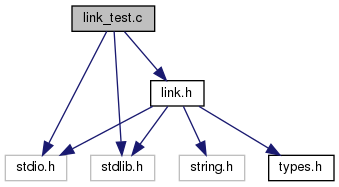
\includegraphics[width=327pt]{link__test_8c__incl}
\end{center}
\end{figure}
\subsection*{Functions}
\begin{DoxyCompactItemize}
\item 
int \hyperlink{link__test_8c_ae66f6b31b5ad750f1fe042a706a4e3d4}{main} ()
\begin{DoxyCompactList}\small\item\em funcion principal de prueba del link \end{DoxyCompactList}\end{DoxyCompactItemize}


\subsection{Detailed Description}
En este fichero probamos las funciones del link. 

\begin{DoxyAuthor}{Author}
Manuel Suarez, Saul Almazán, Álvaro Becerra, Rodrigo Lardiés 
\end{DoxyAuthor}
\begin{DoxyVersion}{Version}
1.\+0 
\end{DoxyVersion}
\begin{DoxyDate}{Date}
15/11/2018 
\end{DoxyDate}


\subsection{Function Documentation}
\mbox{\Hypertarget{link__test_8c_ae66f6b31b5ad750f1fe042a706a4e3d4}\label{link__test_8c_ae66f6b31b5ad750f1fe042a706a4e3d4}} 
\index{link\+\_\+test.\+c@{link\+\_\+test.\+c}!main@{main}}
\index{main@{main}!link\+\_\+test.\+c@{link\+\_\+test.\+c}}
\subsubsection{\texorpdfstring{main()}{main()}}
{\footnotesize\ttfamily int main (\begin{DoxyParamCaption}{ }\end{DoxyParamCaption})}



funcion principal de prueba del link 

\begin{DoxyAuthor}{Author}
Manuel Suarez, Saul Almazán, Álvaro Becerra, Rodrigo Lardiés 
\end{DoxyAuthor}
\begin{DoxyDate}{Date}
10/11/2018 
\end{DoxyDate}
\begin{DoxyReturn}{Returns}
int 
\end{DoxyReturn}

\hypertarget{object_8c}{}\section{object.\+c File Reference}
\label{object_8c}\index{object.\+c@{object.\+c}}


En este fichero implementamos las funciones del objeto.  


{\ttfamily \#include $<$stdio.\+h$>$}\newline
{\ttfamily \#include $<$stdlib.\+h$>$}\newline
{\ttfamily \#include $<$string.\+h$>$}\newline
{\ttfamily \#include \char`\"{}object.\+h\char`\"{}}\newline
Include dependency graph for object.\+c\+:\nopagebreak
\begin{figure}[H]
\begin{center}
\leavevmode
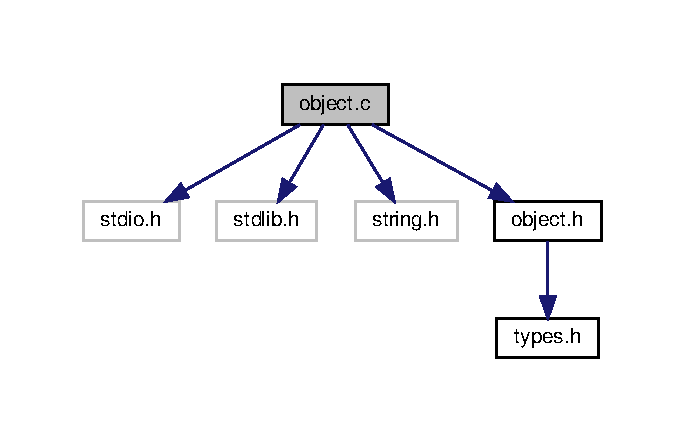
\includegraphics[width=329pt]{object_8c__incl}
\end{center}
\end{figure}
\subsection*{Classes}
\begin{DoxyCompactItemize}
\item 
struct \hyperlink{struct__Object}{\+\_\+\+Object}
\end{DoxyCompactItemize}
\subsection*{Functions}
\begin{DoxyCompactItemize}
\item 
\hyperlink{object_8h_a7f8bbcda919b65ce67f92fba08e0212f}{Object} $\ast$ \hyperlink{object_8c_a2dd568a27239e988cdde871cfb30e166}{object\+\_\+create} ()
\begin{DoxyCompactList}\small\item\em crea un objeto \end{DoxyCompactList}\item 
void \hyperlink{object_8c_a2f26d467bceeedc73132eff682bdeb76}{object\+\_\+destroy} (\hyperlink{object_8h_a7f8bbcda919b65ce67f92fba08e0212f}{Object} $\ast$object)
\begin{DoxyCompactList}\small\item\em destruye un objeto \end{DoxyCompactList}\item 
\hyperlink{types_8h_a845e604fb28f7e3d97549da3448149d3}{Id} \hyperlink{object_8c_ac5af152381a21853c6a28cc120e8e7fe}{object\+\_\+get\+\_\+id} (\hyperlink{object_8h_a7f8bbcda919b65ce67f92fba08e0212f}{Object} $\ast$object)
\begin{DoxyCompactList}\small\item\em devuelve el Id de un objeto \end{DoxyCompactList}\item 
char $\ast$ \hyperlink{object_8c_a7954dbdd53d8b5dc259993f04bba28f8}{object\+\_\+get\+\_\+name} (\hyperlink{object_8h_a7f8bbcda919b65ce67f92fba08e0212f}{Object} $\ast$object)
\begin{DoxyCompactList}\small\item\em devuelve el nombre de un objeto \end{DoxyCompactList}\item 
char $\ast$ \hyperlink{object_8c_ab92f583fcb6e3000ebe48cc04c5853cd}{object\+\_\+get\+\_\+description} (\hyperlink{object_8h_a7f8bbcda919b65ce67f92fba08e0212f}{Object} $\ast$object)
\begin{DoxyCompactList}\small\item\em devuelve la descripcion de un objeto \end{DoxyCompactList}\item 
\hyperlink{types_8h_a32c27cc471df37f4fc818d65de0a56c4}{S\+T\+A\+T\+US} \hyperlink{object_8c_a583e26f5ce36b881294544c2e5751545}{object\+\_\+set\+\_\+id} (\hyperlink{object_8h_a7f8bbcda919b65ce67f92fba08e0212f}{Object} $\ast$object, \hyperlink{types_8h_a845e604fb28f7e3d97549da3448149d3}{Id} nuevo\+\_\+id)
\begin{DoxyCompactList}\small\item\em modifica el id de un objeto \end{DoxyCompactList}\item 
\hyperlink{types_8h_a32c27cc471df37f4fc818d65de0a56c4}{S\+T\+A\+T\+US} \hyperlink{object_8c_ae88627a8873d8f08fba9c0470a19cfc0}{object\+\_\+set\+\_\+description} (\hyperlink{object_8h_a7f8bbcda919b65ce67f92fba08e0212f}{Object} $\ast$object, char $\ast$description)
\begin{DoxyCompactList}\small\item\em modifica la descripcion de un objeto \end{DoxyCompactList}\item 
\hyperlink{types_8h_a32c27cc471df37f4fc818d65de0a56c4}{S\+T\+A\+T\+US} \hyperlink{object_8c_a7380846ad2114ea6c10087dbbd48b672}{object\+\_\+set\+\_\+name} (\hyperlink{object_8h_a7f8bbcda919b65ce67f92fba08e0212f}{Object} $\ast$object, char $\ast$nuevo\+\_\+nombre)
\begin{DoxyCompactList}\small\item\em modifica el nombre de un objeto \end{DoxyCompactList}\item 
int \hyperlink{object_8c_a9706d7bb1dd6b0a322ffeef034f65e0e}{object\+\_\+print} (F\+I\+LE $\ast$f, \hyperlink{object_8h_a7f8bbcda919b65ce67f92fba08e0212f}{Object} $\ast$object)
\begin{DoxyCompactList}\small\item\em imprime un objeto \end{DoxyCompactList}\end{DoxyCompactItemize}


\subsection{Detailed Description}
En este fichero implementamos las funciones del objeto. 

\begin{DoxyAuthor}{Author}
Manuel Suarez, Saul Almazán, Álvaro Becerra, Rodrigo Lardiés 
\end{DoxyAuthor}
\begin{DoxyVersion}{Version}
1.\+0 
\end{DoxyVersion}
\begin{DoxyDate}{Date}
20/10/2018 
\end{DoxyDate}


\subsection{Function Documentation}
\mbox{\Hypertarget{object_8c_a2dd568a27239e988cdde871cfb30e166}\label{object_8c_a2dd568a27239e988cdde871cfb30e166}} 
\index{object.\+c@{object.\+c}!object\+\_\+create@{object\+\_\+create}}
\index{object\+\_\+create@{object\+\_\+create}!object.\+c@{object.\+c}}
\subsubsection{\texorpdfstring{object\+\_\+create()}{object\_create()}}
{\footnotesize\ttfamily \hyperlink{object_8h_a7f8bbcda919b65ce67f92fba08e0212f}{Object}$\ast$ object\+\_\+create (\begin{DoxyParamCaption}{ }\end{DoxyParamCaption})}



crea un objeto 

\begin{DoxyAuthor}{Author}
Manuel Suarez, Saul Almazán, Álvaro Becerra, Rodrigo Lardiés 
\end{DoxyAuthor}
\begin{DoxyDate}{Date}
20/10/2018 
\end{DoxyDate}
\begin{DoxyReturn}{Returns}
Object (El objeto que crea) 
\end{DoxyReturn}
\mbox{\Hypertarget{object_8c_a2f26d467bceeedc73132eff682bdeb76}\label{object_8c_a2f26d467bceeedc73132eff682bdeb76}} 
\index{object.\+c@{object.\+c}!object\+\_\+destroy@{object\+\_\+destroy}}
\index{object\+\_\+destroy@{object\+\_\+destroy}!object.\+c@{object.\+c}}
\subsubsection{\texorpdfstring{object\+\_\+destroy()}{object\_destroy()}}
{\footnotesize\ttfamily void object\+\_\+destroy (\begin{DoxyParamCaption}\item[{\hyperlink{object_8h_a7f8bbcda919b65ce67f92fba08e0212f}{Object} $\ast$}]{object }\end{DoxyParamCaption})}



destruye un objeto 

\begin{DoxyAuthor}{Author}
Manuel Suarez, Saul Almazán, Álvaro Becerra, Rodrigo Lardiés 
\end{DoxyAuthor}
\begin{DoxyDate}{Date}
20/10/2018 
\end{DoxyDate}

\begin{DoxyParams}{Parameters}
{\em object} & (Objeto a destruir) \\
\hline
\end{DoxyParams}
\begin{DoxyReturn}{Returns}
void (no devuelve nada) 
\end{DoxyReturn}
\mbox{\Hypertarget{object_8c_ab92f583fcb6e3000ebe48cc04c5853cd}\label{object_8c_ab92f583fcb6e3000ebe48cc04c5853cd}} 
\index{object.\+c@{object.\+c}!object\+\_\+get\+\_\+description@{object\+\_\+get\+\_\+description}}
\index{object\+\_\+get\+\_\+description@{object\+\_\+get\+\_\+description}!object.\+c@{object.\+c}}
\subsubsection{\texorpdfstring{object\+\_\+get\+\_\+description()}{object\_get\_description()}}
{\footnotesize\ttfamily char$\ast$ object\+\_\+get\+\_\+description (\begin{DoxyParamCaption}\item[{\hyperlink{object_8h_a7f8bbcda919b65ce67f92fba08e0212f}{Object} $\ast$}]{object }\end{DoxyParamCaption})}



devuelve la descripcion de un objeto 

\begin{DoxyAuthor}{Author}
Manuel Suarez, Saul Almazán, Álvaro Becerra, Rodrigo Lardiés 
\end{DoxyAuthor}
\begin{DoxyDate}{Date}
20/10/2018 
\end{DoxyDate}

\begin{DoxyParams}{Parameters}
{\em object} & (Objeto a usar) \\
\hline
\end{DoxyParams}
\begin{DoxyReturn}{Returns}
char (descripcion del objeto) 
\end{DoxyReturn}
\mbox{\Hypertarget{object_8c_ac5af152381a21853c6a28cc120e8e7fe}\label{object_8c_ac5af152381a21853c6a28cc120e8e7fe}} 
\index{object.\+c@{object.\+c}!object\+\_\+get\+\_\+id@{object\+\_\+get\+\_\+id}}
\index{object\+\_\+get\+\_\+id@{object\+\_\+get\+\_\+id}!object.\+c@{object.\+c}}
\subsubsection{\texorpdfstring{object\+\_\+get\+\_\+id()}{object\_get\_id()}}
{\footnotesize\ttfamily \hyperlink{types_8h_a845e604fb28f7e3d97549da3448149d3}{Id} object\+\_\+get\+\_\+id (\begin{DoxyParamCaption}\item[{\hyperlink{object_8h_a7f8bbcda919b65ce67f92fba08e0212f}{Object} $\ast$}]{object }\end{DoxyParamCaption})}



devuelve el Id de un objeto 

\begin{DoxyAuthor}{Author}
Manuel Suarez, Saul Almazán, Álvaro Becerra, Rodrigo Lardiés 
\end{DoxyAuthor}
\begin{DoxyDate}{Date}
20/10/2018 
\end{DoxyDate}

\begin{DoxyParams}{Parameters}
{\em object} & (Objeto a usar) \\
\hline
\end{DoxyParams}
\begin{DoxyReturn}{Returns}
Id (Id del objeto) 
\end{DoxyReturn}
\mbox{\Hypertarget{object_8c_a7954dbdd53d8b5dc259993f04bba28f8}\label{object_8c_a7954dbdd53d8b5dc259993f04bba28f8}} 
\index{object.\+c@{object.\+c}!object\+\_\+get\+\_\+name@{object\+\_\+get\+\_\+name}}
\index{object\+\_\+get\+\_\+name@{object\+\_\+get\+\_\+name}!object.\+c@{object.\+c}}
\subsubsection{\texorpdfstring{object\+\_\+get\+\_\+name()}{object\_get\_name()}}
{\footnotesize\ttfamily char$\ast$ object\+\_\+get\+\_\+name (\begin{DoxyParamCaption}\item[{\hyperlink{object_8h_a7f8bbcda919b65ce67f92fba08e0212f}{Object} $\ast$}]{object }\end{DoxyParamCaption})}



devuelve el nombre de un objeto 

\begin{DoxyAuthor}{Author}
Manuel Suarez, Saul Almazán, Álvaro Becerra, Rodrigo Lardiés 
\end{DoxyAuthor}
\begin{DoxyDate}{Date}
20/10/2018 
\end{DoxyDate}

\begin{DoxyParams}{Parameters}
{\em object} & (Objeto a usar) \\
\hline
\end{DoxyParams}
\begin{DoxyReturn}{Returns}
char (nombre del objeto) 
\end{DoxyReturn}
\mbox{\Hypertarget{object_8c_a9706d7bb1dd6b0a322ffeef034f65e0e}\label{object_8c_a9706d7bb1dd6b0a322ffeef034f65e0e}} 
\index{object.\+c@{object.\+c}!object\+\_\+print@{object\+\_\+print}}
\index{object\+\_\+print@{object\+\_\+print}!object.\+c@{object.\+c}}
\subsubsection{\texorpdfstring{object\+\_\+print()}{object\_print()}}
{\footnotesize\ttfamily int object\+\_\+print (\begin{DoxyParamCaption}\item[{F\+I\+LE $\ast$}]{f,  }\item[{\hyperlink{object_8h_a7f8bbcda919b65ce67f92fba08e0212f}{Object} $\ast$}]{object }\end{DoxyParamCaption})}



imprime un objeto 

\begin{DoxyAuthor}{Author}
Manuel Suarez, Saul Almazán, Álvaro Becerra, Rodrigo Lardiés 
\end{DoxyAuthor}
\begin{DoxyDate}{Date}
20/10/2018 
\end{DoxyDate}

\begin{DoxyParams}{Parameters}
{\em object} & (Objeto a usar) \\
\hline
{\em f} & (donde se imprime) \\
\hline
\end{DoxyParams}
\begin{DoxyReturn}{Returns}
int (-\/1 si hay algun error) 
\end{DoxyReturn}
\mbox{\Hypertarget{object_8c_ae88627a8873d8f08fba9c0470a19cfc0}\label{object_8c_ae88627a8873d8f08fba9c0470a19cfc0}} 
\index{object.\+c@{object.\+c}!object\+\_\+set\+\_\+description@{object\+\_\+set\+\_\+description}}
\index{object\+\_\+set\+\_\+description@{object\+\_\+set\+\_\+description}!object.\+c@{object.\+c}}
\subsubsection{\texorpdfstring{object\+\_\+set\+\_\+description()}{object\_set\_description()}}
{\footnotesize\ttfamily \hyperlink{types_8h_a32c27cc471df37f4fc818d65de0a56c4}{S\+T\+A\+T\+US} object\+\_\+set\+\_\+description (\begin{DoxyParamCaption}\item[{\hyperlink{object_8h_a7f8bbcda919b65ce67f92fba08e0212f}{Object} $\ast$}]{object,  }\item[{char $\ast$}]{description }\end{DoxyParamCaption})}



modifica la descripcion de un objeto 

\begin{DoxyAuthor}{Author}
Manuel Suarez, Saul Almazán, Álvaro Becerra, Rodrigo Lardiés 
\end{DoxyAuthor}
\begin{DoxyDate}{Date}
20/10/2018 
\end{DoxyDate}

\begin{DoxyParams}{Parameters}
{\em object} & (Objeto a modificar) \\
\hline
{\em description} & (Nueva descripcion) \\
\hline
\end{DoxyParams}
\begin{DoxyReturn}{Returns}
S\+T\+A\+T\+US (OK si se realiza con exito o E\+R\+R\+OR de lo contrario) 
\end{DoxyReturn}
\mbox{\Hypertarget{object_8c_a583e26f5ce36b881294544c2e5751545}\label{object_8c_a583e26f5ce36b881294544c2e5751545}} 
\index{object.\+c@{object.\+c}!object\+\_\+set\+\_\+id@{object\+\_\+set\+\_\+id}}
\index{object\+\_\+set\+\_\+id@{object\+\_\+set\+\_\+id}!object.\+c@{object.\+c}}
\subsubsection{\texorpdfstring{object\+\_\+set\+\_\+id()}{object\_set\_id()}}
{\footnotesize\ttfamily \hyperlink{types_8h_a32c27cc471df37f4fc818d65de0a56c4}{S\+T\+A\+T\+US} object\+\_\+set\+\_\+id (\begin{DoxyParamCaption}\item[{\hyperlink{object_8h_a7f8bbcda919b65ce67f92fba08e0212f}{Object} $\ast$}]{object,  }\item[{\hyperlink{types_8h_a845e604fb28f7e3d97549da3448149d3}{Id}}]{nuevo\+\_\+id }\end{DoxyParamCaption})}



modifica el id de un objeto 

\begin{DoxyAuthor}{Author}
Manuel Suarez, Saul Almazán, Álvaro Becerra, Rodrigo Lardiés 
\end{DoxyAuthor}
\begin{DoxyDate}{Date}
20/10/2018 
\end{DoxyDate}

\begin{DoxyParams}{Parameters}
{\em object} & (Objeto a modificar) \\
\hline
{\em nuevo\+\_\+id} & (Id nuevo del objeto) \\
\hline
\end{DoxyParams}
\begin{DoxyReturn}{Returns}
S\+T\+A\+T\+US (OK si se realiza con exito o E\+R\+R\+OR de lo contrario) 
\end{DoxyReturn}
\mbox{\Hypertarget{object_8c_a7380846ad2114ea6c10087dbbd48b672}\label{object_8c_a7380846ad2114ea6c10087dbbd48b672}} 
\index{object.\+c@{object.\+c}!object\+\_\+set\+\_\+name@{object\+\_\+set\+\_\+name}}
\index{object\+\_\+set\+\_\+name@{object\+\_\+set\+\_\+name}!object.\+c@{object.\+c}}
\subsubsection{\texorpdfstring{object\+\_\+set\+\_\+name()}{object\_set\_name()}}
{\footnotesize\ttfamily \hyperlink{types_8h_a32c27cc471df37f4fc818d65de0a56c4}{S\+T\+A\+T\+US} object\+\_\+set\+\_\+name (\begin{DoxyParamCaption}\item[{\hyperlink{object_8h_a7f8bbcda919b65ce67f92fba08e0212f}{Object} $\ast$}]{object,  }\item[{char $\ast$}]{nuevo\+\_\+nombre }\end{DoxyParamCaption})}



modifica el nombre de un objeto 

\begin{DoxyAuthor}{Author}
Manuel Suarez, Saul Almazán, Álvaro Becerra, Rodrigo Lardiés 
\end{DoxyAuthor}
\begin{DoxyDate}{Date}
20/10/2018 
\end{DoxyDate}

\begin{DoxyParams}{Parameters}
{\em object} & (Objeto a modificar) \\
\hline
{\em nuevo\+\_\+nombre} & (Nuevo nombre) \\
\hline
\end{DoxyParams}
\begin{DoxyReturn}{Returns}
S\+T\+A\+T\+US (OK si se realiza con exito o E\+R\+R\+OR de lo contrario) 
\end{DoxyReturn}

\hypertarget{object__test_8c}{}\section{src/object\+\_\+test.c File Reference}
\label{object__test_8c}\index{src/object\+\_\+test.\+c@{src/object\+\_\+test.\+c}}


Prueba del modulo object.  


{\ttfamily \#include $<$stdio.\+h$>$}\newline
{\ttfamily \#include $<$stdlib.\+h$>$}\newline
{\ttfamily \#include $<$string.\+h$>$}\newline
{\ttfamily \#include \char`\"{}object.\+h\char`\"{}}\newline
{\ttfamily \#include \char`\"{}object\+\_\+test.\+h\char`\"{}}\newline
{\ttfamily \#include \char`\"{}test.\+h\char`\"{}}\newline
Include dependency graph for object\+\_\+test.\+c\+:
% FIG 0
\subsection*{Macros}
\begin{DoxyCompactItemize}
\item 
\#define \hyperlink{object__test_8c_a2a77d2f2c5b698c69c19e1f8782bf709}{M\+A\+X\+\_\+\+T\+E\+S\+TS}~41
\end{DoxyCompactItemize}
\subsection*{Functions}
\begin{DoxyCompactItemize}
\item 
int \hyperlink{object__test_8c_a3c04138a5bfe5d72780bb7e82a18e627}{main} (int argc, char $\ast$$\ast$argv)
\begin{DoxyCompactList}\small\item\em Funcion principal de pruebas para el modulo object. \end{DoxyCompactList}\item 
void \hyperlink{object__test_8c_a3836d69f92ce7149d56bafcaec83f516}{test1\+\_\+object\+\_\+create} ()
\item 
void \hyperlink{object__test_8c_a74e25ad653c4a32b9922fff8e4f916fd}{test1\+\_\+object\+\_\+set\+\_\+name} ()
\item 
void \hyperlink{object__test_8c_acf42b7e7be91ede243f2aaa56c4c9347}{test2\+\_\+object\+\_\+set\+\_\+name} ()
\item 
void \hyperlink{object__test_8c_ab40669b5d083b6484197d917fb6882b1}{test3\+\_\+object\+\_\+set\+\_\+name} ()
\item 
void \hyperlink{object__test_8c_a6f19ebf6034115c2cdcc3c7bfea25964}{test1\+\_\+object\+\_\+set\+\_\+id} ()
\item 
void \hyperlink{object__test_8c_a9ada47d4e8c46f0f3374b2fa66d6430c}{test2\+\_\+object\+\_\+set\+\_\+north} ()
\item 
void \hyperlink{object__test_8c_a3418e1bc1ae952d49085a68375940ef6}{test1\+\_\+object\+\_\+set\+\_\+south} ()
\item 
void \hyperlink{object__test_8c_aa606c3fb296b209d5165b0c45a322fec}{test2\+\_\+object\+\_\+set\+\_\+south} ()
\item 
void \hyperlink{object__test_8c_a0da5b8050f929cbcfa8a759a962856f5}{test1\+\_\+object\+\_\+set\+\_\+east} ()
\item 
void \hyperlink{object__test_8c_a6d5475cf455fe37de66ccca9fd2187dc}{test2\+\_\+object\+\_\+set\+\_\+east} ()
\item 
void \hyperlink{object__test_8c_a7f0c6a44fb6b1010810050f2ea72dc69}{test1\+\_\+object\+\_\+set\+\_\+west} ()
\item 
void \hyperlink{object__test_8c_a79539ace87f072f2722181db52004696}{test2\+\_\+object\+\_\+set\+\_\+west} ()
\item 
void \hyperlink{object__test_8c_ad2411bc3cc47c9905e63a3d9c561d369}{test1\+\_\+object\+\_\+get\+\_\+name} ()
\item 
void \hyperlink{object__test_8c_abdfafbc7b8588d3dcdb05fd2beb2397e}{test2\+\_\+object\+\_\+get\+\_\+name} ()
\item 
void \hyperlink{object__test_8c_a8476950bc3a7d77a95a393acec4a9f7a}{test1\+\_\+object\+\_\+take\+\_\+object} ()
\item 
void \hyperlink{object__test_8c_a0bd507dfdefd8223c1c0d5c8aeb44d23}{test2\+\_\+object\+\_\+take\+\_\+object} ()
\item 
void \hyperlink{object__test_8c_add7988c5f1529d05be42760049c5b554}{test3\+\_\+object\+\_\+take\+\_\+object} ()
\item 
void \hyperlink{object__test_8c_acedfe61e854500c485598d66b7e5096c}{test1\+\_\+object\+\_\+get\+\_\+north} ()
\item 
void \hyperlink{object__test_8c_a098d0c4e35b24e3b126575e47c76e523}{test2\+\_\+object\+\_\+get\+\_\+north} ()
\item 
void \hyperlink{object__test_8c_a2e91b10e48cc9dc38285a3e358650e80}{test1\+\_\+object\+\_\+get\+\_\+south} ()
\item 
void \hyperlink{object__test_8c_a84bb6c22cdec27962fe5a6b81e41010b}{test2\+\_\+object\+\_\+get\+\_\+south} ()
\item 
void \hyperlink{object__test_8c_add870347717b28f9627efc66ddb5a12b}{test1\+\_\+object\+\_\+get\+\_\+east} ()
\item 
void \hyperlink{object__test_8c_a0af301322234ef610275643ea846ec67}{test2\+\_\+object\+\_\+get\+\_\+east} ()
\item 
void \hyperlink{object__test_8c_a8375fd84bcc6e4a2427cf4f6a77e102d}{test1\+\_\+object\+\_\+get\+\_\+west} ()
\item 
void \hyperlink{object__test_8c_a3e8525c0760af6b2bed97b3e81592fa9}{test2\+\_\+object\+\_\+get\+\_\+west} ()
\item 
void \hyperlink{object__test_8c_aa88e9e9dab92ba9c58851d7a7a8415f0}{test1\+\_\+object\+\_\+get\+\_\+id} ()
\item 
void \hyperlink{object__test_8c_a1ff250f0f43297f57fcce1f3a6ae490b}{test2\+\_\+object\+\_\+get\+\_\+id} ()
\item 
void \hyperlink{object__test_8c_a90c957b12175892a0dacc4e61f3c2ec2}{test1\+\_\+object\+\_\+leave\+\_\+object} ()
\item 
void \hyperlink{object__test_8c_a934818c30bc94f423633661c38c73f2a}{test2\+\_\+object\+\_\+leave\+\_\+object} ()
\item 
void \hyperlink{object__test_8c_ade12664b9bc4400080ba40f8db7105aa}{test1\+\_\+object\+\_\+set\+\_\+gdesc} ()
\item 
void \hyperlink{object__test_8c_af8a5fe8a62dfe35363d287574bac56c1}{test2\+\_\+object\+\_\+set\+\_\+gdesc} ()
\item 
void \hyperlink{object__test_8c_a43375c48c794bb6b2ed3fb8d949149b5}{test1\+\_\+object\+\_\+get\+\_\+gdesc} ()
\item 
void \hyperlink{object__test_8c_a986fccb3aa7593b75b043547e9e22ebb}{test2\+\_\+object\+\_\+get\+\_\+gdesc} ()
\item 
void \hyperlink{object__test_8c_afb26b8c66d332354df8bfd57a8033b8f}{test1\+\_\+object\+\_\+set\+\_\+description} ()
\item 
void \hyperlink{object__test_8c_a65e32c3642c1d9207cdd84b134c616da}{test2\+\_\+object\+\_\+set\+\_\+description} ()
\item 
void \hyperlink{object__test_8c_afe180b78a201df7bc1629701db1d464c}{test1\+\_\+object\+\_\+get\+\_\+description} ()
\item 
void \hyperlink{object__test_8c_a35d9a40796133791c157c044ea1cef85}{test2\+\_\+object\+\_\+get\+\_\+description} ()
\end{DoxyCompactItemize}


\subsection{Detailed Description}
Prueba del modulo object. 

\begin{DoxyAuthor}{Author}
Manuel Suarez, Saul Almazán, �?lvaro Becerra, Rodrigo Lardiés 
\end{DoxyAuthor}
\begin{DoxyVersion}{Version}
1.\+0 
\end{DoxyVersion}
\begin{DoxyDate}{Date}
12-\/11-\/2018 
\end{DoxyDate}


\subsection{Macro Definition Documentation}
\mbox{\Hypertarget{object__test_8c_a2a77d2f2c5b698c69c19e1f8782bf709}\label{object__test_8c_a2a77d2f2c5b698c69c19e1f8782bf709}} 
\index{object\+\_\+test.\+c@{object\+\_\+test.\+c}!M\+A\+X\+\_\+\+T\+E\+S\+TS@{M\+A\+X\+\_\+\+T\+E\+S\+TS}}
\index{M\+A\+X\+\_\+\+T\+E\+S\+TS@{M\+A\+X\+\_\+\+T\+E\+S\+TS}!object\+\_\+test.\+c@{object\+\_\+test.\+c}}
\subsubsection{\texorpdfstring{M\+A\+X\+\_\+\+T\+E\+S\+TS}{MAX\_TESTS}}
{\footnotesize\ttfamily \#define M\+A\+X\+\_\+\+T\+E\+S\+TS~41}

T\+A\+M\+\_\+\+T\+E\+S\+TS 

\subsection{Function Documentation}
\mbox{\Hypertarget{object__test_8c_a3c04138a5bfe5d72780bb7e82a18e627}\label{object__test_8c_a3c04138a5bfe5d72780bb7e82a18e627}} 
\index{object\+\_\+test.\+c@{object\+\_\+test.\+c}!main@{main}}
\index{main@{main}!object\+\_\+test.\+c@{object\+\_\+test.\+c}}
\subsubsection{\texorpdfstring{main()}{main()}}
{\footnotesize\ttfamily int main (\begin{DoxyParamCaption}\item[{int}]{argc,  }\item[{char $\ast$$\ast$}]{argv }\end{DoxyParamCaption})}



Funcion principal de pruebas para el modulo object. 

Dos modos de ejecucion\+: 1.-\/\+Si se ejecuta sin parametros se ejecutan todas las pruebas 2.-\/\+Si se ejecuta con un numero entre 1 y el numero de pruebas solo ejecuta la prueba indicada \mbox{\Hypertarget{object__test_8c_a3836d69f92ce7149d56bafcaec83f516}\label{object__test_8c_a3836d69f92ce7149d56bafcaec83f516}} 
\index{object\+\_\+test.\+c@{object\+\_\+test.\+c}!test1\+\_\+object\+\_\+create@{test1\+\_\+object\+\_\+create}}
\index{test1\+\_\+object\+\_\+create@{test1\+\_\+object\+\_\+create}!object\+\_\+test.\+c@{object\+\_\+test.\+c}}
\subsubsection{\texorpdfstring{test1\+\_\+object\+\_\+create()}{test1\_object\_create()}}
{\footnotesize\ttfamily void test1\+\_\+object\+\_\+create (\begin{DoxyParamCaption}{ }\end{DoxyParamCaption})}

\begin{DoxyRefDesc}{Test}
\item[\hyperlink{test__test000047}{Test}]Prueba la función de creación de un objeto \end{DoxyRefDesc}
\begin{DoxyPrecond}{Precondition}
Nada 
\end{DoxyPrecond}
\begin{DoxyPostcond}{Postcondition}
Un puntero no nulo al objeto creado 
\end{DoxyPostcond}
\mbox{\Hypertarget{object__test_8c_afe180b78a201df7bc1629701db1d464c}\label{object__test_8c_afe180b78a201df7bc1629701db1d464c}} 
\index{object\+\_\+test.\+c@{object\+\_\+test.\+c}!test1\+\_\+object\+\_\+get\+\_\+description@{test1\+\_\+object\+\_\+get\+\_\+description}}
\index{test1\+\_\+object\+\_\+get\+\_\+description@{test1\+\_\+object\+\_\+get\+\_\+description}!object\+\_\+test.\+c@{object\+\_\+test.\+c}}
\subsubsection{\texorpdfstring{test1\+\_\+object\+\_\+get\+\_\+description()}{test1\_object\_get\_description()}}
{\footnotesize\ttfamily void test1\+\_\+object\+\_\+get\+\_\+description (\begin{DoxyParamCaption}{ }\end{DoxyParamCaption})}

\begin{DoxyRefDesc}{Test}
\item[\hyperlink{test__test000082}{Test}]Prueba la función para obtener una descripcion en un objeto \end{DoxyRefDesc}
\begin{DoxyPrecond}{Precondition}
objeto con una descripcion 
\end{DoxyPrecond}
\begin{DoxyPostcond}{Postcondition}
La salida debe ser una comparación de cadenas igual a 0 
\end{DoxyPostcond}
\mbox{\Hypertarget{object__test_8c_add870347717b28f9627efc66ddb5a12b}\label{object__test_8c_add870347717b28f9627efc66ddb5a12b}} 
\index{object\+\_\+test.\+c@{object\+\_\+test.\+c}!test1\+\_\+object\+\_\+get\+\_\+east@{test1\+\_\+object\+\_\+get\+\_\+east}}
\index{test1\+\_\+object\+\_\+get\+\_\+east@{test1\+\_\+object\+\_\+get\+\_\+east}!object\+\_\+test.\+c@{object\+\_\+test.\+c}}
\subsubsection{\texorpdfstring{test1\+\_\+object\+\_\+get\+\_\+east()}{test1\_object\_get\_east()}}
{\footnotesize\ttfamily void test1\+\_\+object\+\_\+get\+\_\+east (\begin{DoxyParamCaption}{ }\end{DoxyParamCaption})}

\begin{DoxyRefDesc}{Test}
\item[\hyperlink{test__test000068}{Test}]Prueba la función para obtener el este de un objeto \end{DoxyRefDesc}
\begin{DoxyPrecond}{Precondition}
objeto con este asignado 
\end{DoxyPrecond}
\begin{DoxyPostcond}{Postcondition}
La salida debe ser id=4 
\end{DoxyPostcond}
\mbox{\Hypertarget{object__test_8c_a43375c48c794bb6b2ed3fb8d949149b5}\label{object__test_8c_a43375c48c794bb6b2ed3fb8d949149b5}} 
\index{object\+\_\+test.\+c@{object\+\_\+test.\+c}!test1\+\_\+object\+\_\+get\+\_\+gdesc@{test1\+\_\+object\+\_\+get\+\_\+gdesc}}
\index{test1\+\_\+object\+\_\+get\+\_\+gdesc@{test1\+\_\+object\+\_\+get\+\_\+gdesc}!object\+\_\+test.\+c@{object\+\_\+test.\+c}}
\subsubsection{\texorpdfstring{test1\+\_\+object\+\_\+get\+\_\+gdesc()}{test1\_object\_get\_gdesc()}}
{\footnotesize\ttfamily void test1\+\_\+object\+\_\+get\+\_\+gdesc (\begin{DoxyParamCaption}{ }\end{DoxyParamCaption})}

\begin{DoxyRefDesc}{Test}
\item[\hyperlink{test__test000078}{Test}]Prueba la función para dejar un obtener un dibujo en un objeto \end{DoxyRefDesc}
\begin{DoxyPrecond}{Precondition}
objeto con dibujo 
\end{DoxyPrecond}
\begin{DoxyPostcond}{Postcondition}
La salida debe ser una comparacion de cadenas igual a 0 
\end{DoxyPostcond}
\mbox{\Hypertarget{object__test_8c_aa88e9e9dab92ba9c58851d7a7a8415f0}\label{object__test_8c_aa88e9e9dab92ba9c58851d7a7a8415f0}} 
\index{object\+\_\+test.\+c@{object\+\_\+test.\+c}!test1\+\_\+object\+\_\+get\+\_\+id@{test1\+\_\+object\+\_\+get\+\_\+id}}
\index{test1\+\_\+object\+\_\+get\+\_\+id@{test1\+\_\+object\+\_\+get\+\_\+id}!object\+\_\+test.\+c@{object\+\_\+test.\+c}}
\subsubsection{\texorpdfstring{test1\+\_\+object\+\_\+get\+\_\+id()}{test1\_object\_get\_id()}}
{\footnotesize\ttfamily void test1\+\_\+object\+\_\+get\+\_\+id (\begin{DoxyParamCaption}{ }\end{DoxyParamCaption})}

\begin{DoxyRefDesc}{Test}
\item[\hyperlink{test__test000072}{Test}]Prueba la función para obtener el id de un objeto \end{DoxyRefDesc}
\begin{DoxyPrecond}{Precondition}
objeto con id asignado 
\end{DoxyPrecond}
\begin{DoxyPostcond}{Postcondition}
La salida debe ser id=5 
\end{DoxyPostcond}
\mbox{\Hypertarget{object__test_8c_ad2411bc3cc47c9905e63a3d9c561d369}\label{object__test_8c_ad2411bc3cc47c9905e63a3d9c561d369}} 
\index{object\+\_\+test.\+c@{object\+\_\+test.\+c}!test1\+\_\+object\+\_\+get\+\_\+name@{test1\+\_\+object\+\_\+get\+\_\+name}}
\index{test1\+\_\+object\+\_\+get\+\_\+name@{test1\+\_\+object\+\_\+get\+\_\+name}!object\+\_\+test.\+c@{object\+\_\+test.\+c}}
\subsubsection{\texorpdfstring{test1\+\_\+object\+\_\+get\+\_\+name()}{test1\_object\_get\_name()}}
{\footnotesize\ttfamily void test1\+\_\+object\+\_\+get\+\_\+name (\begin{DoxyParamCaption}{ }\end{DoxyParamCaption})}

\begin{DoxyRefDesc}{Test}
\item[\hyperlink{test__test000059}{Test}]Prueba la función para obtener el nombre de un objeto \end{DoxyRefDesc}
\begin{DoxyPrecond}{Precondition}
objeto con nombre establecido 
\end{DoxyPrecond}
\begin{DoxyPostcond}{Postcondition}
La salida debe ser una comparación de cadenas igual a 0 
\end{DoxyPostcond}
\mbox{\Hypertarget{object__test_8c_acedfe61e854500c485598d66b7e5096c}\label{object__test_8c_acedfe61e854500c485598d66b7e5096c}} 
\index{object\+\_\+test.\+c@{object\+\_\+test.\+c}!test1\+\_\+object\+\_\+get\+\_\+north@{test1\+\_\+object\+\_\+get\+\_\+north}}
\index{test1\+\_\+object\+\_\+get\+\_\+north@{test1\+\_\+object\+\_\+get\+\_\+north}!object\+\_\+test.\+c@{object\+\_\+test.\+c}}
\subsubsection{\texorpdfstring{test1\+\_\+object\+\_\+get\+\_\+north()}{test1\_object\_get\_north()}}
{\footnotesize\ttfamily void test1\+\_\+object\+\_\+get\+\_\+north (\begin{DoxyParamCaption}{ }\end{DoxyParamCaption})}

\begin{DoxyRefDesc}{Test}
\item[\hyperlink{test__test000064}{Test}]Prueba la función para obtener el norte de un objeto \end{DoxyRefDesc}
\begin{DoxyPrecond}{Precondition}
objeto con norte asignado 
\end{DoxyPrecond}
\begin{DoxyPostcond}{Postcondition}
La salida debe ser id=4 
\end{DoxyPostcond}
\mbox{\Hypertarget{object__test_8c_a2e91b10e48cc9dc38285a3e358650e80}\label{object__test_8c_a2e91b10e48cc9dc38285a3e358650e80}} 
\index{object\+\_\+test.\+c@{object\+\_\+test.\+c}!test1\+\_\+object\+\_\+get\+\_\+south@{test1\+\_\+object\+\_\+get\+\_\+south}}
\index{test1\+\_\+object\+\_\+get\+\_\+south@{test1\+\_\+object\+\_\+get\+\_\+south}!object\+\_\+test.\+c@{object\+\_\+test.\+c}}
\subsubsection{\texorpdfstring{test1\+\_\+object\+\_\+get\+\_\+south()}{test1\_object\_get\_south()}}
{\footnotesize\ttfamily void test1\+\_\+object\+\_\+get\+\_\+south (\begin{DoxyParamCaption}{ }\end{DoxyParamCaption})}

\begin{DoxyRefDesc}{Test}
\item[\hyperlink{test__test000066}{Test}]Prueba la función para obtener el sur de un objeto \end{DoxyRefDesc}
\begin{DoxyPrecond}{Precondition}
objeto con sur asignado 
\end{DoxyPrecond}
\begin{DoxyPostcond}{Postcondition}
La salida debe ser id=4 
\end{DoxyPostcond}
\mbox{\Hypertarget{object__test_8c_a8375fd84bcc6e4a2427cf4f6a77e102d}\label{object__test_8c_a8375fd84bcc6e4a2427cf4f6a77e102d}} 
\index{object\+\_\+test.\+c@{object\+\_\+test.\+c}!test1\+\_\+object\+\_\+get\+\_\+west@{test1\+\_\+object\+\_\+get\+\_\+west}}
\index{test1\+\_\+object\+\_\+get\+\_\+west@{test1\+\_\+object\+\_\+get\+\_\+west}!object\+\_\+test.\+c@{object\+\_\+test.\+c}}
\subsubsection{\texorpdfstring{test1\+\_\+object\+\_\+get\+\_\+west()}{test1\_object\_get\_west()}}
{\footnotesize\ttfamily void test1\+\_\+object\+\_\+get\+\_\+west (\begin{DoxyParamCaption}{ }\end{DoxyParamCaption})}

\begin{DoxyRefDesc}{Test}
\item[\hyperlink{test__test000070}{Test}]Prueba la función para obtener el oeste de un objeto \end{DoxyRefDesc}
\begin{DoxyPrecond}{Precondition}
objeto con oeste asignado 
\end{DoxyPrecond}
\begin{DoxyPostcond}{Postcondition}
La salida debe ser id=4 
\end{DoxyPostcond}
\mbox{\Hypertarget{object__test_8c_a90c957b12175892a0dacc4e61f3c2ec2}\label{object__test_8c_a90c957b12175892a0dacc4e61f3c2ec2}} 
\index{object\+\_\+test.\+c@{object\+\_\+test.\+c}!test1\+\_\+object\+\_\+leave\+\_\+object@{test1\+\_\+object\+\_\+leave\+\_\+object}}
\index{test1\+\_\+object\+\_\+leave\+\_\+object@{test1\+\_\+object\+\_\+leave\+\_\+object}!object\+\_\+test.\+c@{object\+\_\+test.\+c}}
\subsubsection{\texorpdfstring{test1\+\_\+object\+\_\+leave\+\_\+object()}{test1\_object\_leave\_object()}}
{\footnotesize\ttfamily void test1\+\_\+object\+\_\+leave\+\_\+object (\begin{DoxyParamCaption}{ }\end{DoxyParamCaption})}

\begin{DoxyRefDesc}{Test}
\item[\hyperlink{test__test000074}{Test}]Prueba la función para dejar un objeto en un objeto \end{DoxyRefDesc}
\begin{DoxyPrecond}{Precondition}
objeto no N\+U\+LL 
\end{DoxyPrecond}
\begin{DoxyPostcond}{Postcondition}
La salida debe ser OK 
\end{DoxyPostcond}
\mbox{\Hypertarget{object__test_8c_afb26b8c66d332354df8bfd57a8033b8f}\label{object__test_8c_afb26b8c66d332354df8bfd57a8033b8f}} 
\index{object\+\_\+test.\+c@{object\+\_\+test.\+c}!test1\+\_\+object\+\_\+set\+\_\+description@{test1\+\_\+object\+\_\+set\+\_\+description}}
\index{test1\+\_\+object\+\_\+set\+\_\+description@{test1\+\_\+object\+\_\+set\+\_\+description}!object\+\_\+test.\+c@{object\+\_\+test.\+c}}
\subsubsection{\texorpdfstring{test1\+\_\+object\+\_\+set\+\_\+description()}{test1\_object\_set\_description()}}
{\footnotesize\ttfamily void test1\+\_\+object\+\_\+set\+\_\+description (\begin{DoxyParamCaption}{ }\end{DoxyParamCaption})}

\begin{DoxyRefDesc}{Test}
\item[\hyperlink{test__test000080}{Test}]Prueba la función para dejar un establecer una descripcion en un objeto \end{DoxyRefDesc}
\begin{DoxyPrecond}{Precondition}
objeto no N\+U\+LL 
\end{DoxyPrecond}
\begin{DoxyPostcond}{Postcondition}
La salida debe ser OK 
\end{DoxyPostcond}
\mbox{\Hypertarget{object__test_8c_a0da5b8050f929cbcfa8a759a962856f5}\label{object__test_8c_a0da5b8050f929cbcfa8a759a962856f5}} 
\index{object\+\_\+test.\+c@{object\+\_\+test.\+c}!test1\+\_\+object\+\_\+set\+\_\+east@{test1\+\_\+object\+\_\+set\+\_\+east}}
\index{test1\+\_\+object\+\_\+set\+\_\+east@{test1\+\_\+object\+\_\+set\+\_\+east}!object\+\_\+test.\+c@{object\+\_\+test.\+c}}
\subsubsection{\texorpdfstring{test1\+\_\+object\+\_\+set\+\_\+east()}{test1\_object\_set\_east()}}
{\footnotesize\ttfamily void test1\+\_\+object\+\_\+set\+\_\+east (\begin{DoxyParamCaption}{ }\end{DoxyParamCaption})}

\begin{DoxyRefDesc}{Test}
\item[\hyperlink{test__test000055}{Test}]Prueba la función para establecer el este de un objeto \end{DoxyRefDesc}
\begin{DoxyPrecond}{Precondition}
Id a establecer 
\end{DoxyPrecond}
\begin{DoxyPostcond}{Postcondition}
La salida debe ser OK 
\end{DoxyPostcond}
\mbox{\Hypertarget{object__test_8c_ade12664b9bc4400080ba40f8db7105aa}\label{object__test_8c_ade12664b9bc4400080ba40f8db7105aa}} 
\index{object\+\_\+test.\+c@{object\+\_\+test.\+c}!test1\+\_\+object\+\_\+set\+\_\+gdesc@{test1\+\_\+object\+\_\+set\+\_\+gdesc}}
\index{test1\+\_\+object\+\_\+set\+\_\+gdesc@{test1\+\_\+object\+\_\+set\+\_\+gdesc}!object\+\_\+test.\+c@{object\+\_\+test.\+c}}
\subsubsection{\texorpdfstring{test1\+\_\+object\+\_\+set\+\_\+gdesc()}{test1\_object\_set\_gdesc()}}
{\footnotesize\ttfamily void test1\+\_\+object\+\_\+set\+\_\+gdesc (\begin{DoxyParamCaption}{ }\end{DoxyParamCaption})}

\begin{DoxyRefDesc}{Test}
\item[\hyperlink{test__test000076}{Test}]Prueba la función para dejar un establecer un dibujo en un objeto \end{DoxyRefDesc}
\begin{DoxyPrecond}{Precondition}
objeto no N\+U\+LL 
\end{DoxyPrecond}
\begin{DoxyPostcond}{Postcondition}
La salida debe ser OK 
\end{DoxyPostcond}
\mbox{\Hypertarget{object__test_8c_a6f19ebf6034115c2cdcc3c7bfea25964}\label{object__test_8c_a6f19ebf6034115c2cdcc3c7bfea25964}} 
\index{object\+\_\+test.\+c@{object\+\_\+test.\+c}!test1\+\_\+object\+\_\+set\+\_\+id@{test1\+\_\+object\+\_\+set\+\_\+id}}
\index{test1\+\_\+object\+\_\+set\+\_\+id@{test1\+\_\+object\+\_\+set\+\_\+id}!object\+\_\+test.\+c@{object\+\_\+test.\+c}}
\subsubsection{\texorpdfstring{test1\+\_\+object\+\_\+set\+\_\+id()}{test1\_object\_set\_id()}}
{\footnotesize\ttfamily void test1\+\_\+object\+\_\+set\+\_\+id (\begin{DoxyParamCaption}{ }\end{DoxyParamCaption})}

\begin{DoxyRefDesc}{Test}
\item[\hyperlink{test__test000051}{Test}]Prueba la función para establecer el norte de un objeto \end{DoxyRefDesc}
\begin{DoxyPrecond}{Precondition}
Id a establecer 
\end{DoxyPrecond}
\begin{DoxyPostcond}{Postcondition}
La salida debe ser OK 
\end{DoxyPostcond}
\mbox{\Hypertarget{object__test_8c_a74e25ad653c4a32b9922fff8e4f916fd}\label{object__test_8c_a74e25ad653c4a32b9922fff8e4f916fd}} 
\index{object\+\_\+test.\+c@{object\+\_\+test.\+c}!test1\+\_\+object\+\_\+set\+\_\+name@{test1\+\_\+object\+\_\+set\+\_\+name}}
\index{test1\+\_\+object\+\_\+set\+\_\+name@{test1\+\_\+object\+\_\+set\+\_\+name}!object\+\_\+test.\+c@{object\+\_\+test.\+c}}
\subsubsection{\texorpdfstring{test1\+\_\+object\+\_\+set\+\_\+name()}{test1\_object\_set\_name()}}
{\footnotesize\ttfamily void test1\+\_\+object\+\_\+set\+\_\+name (\begin{DoxyParamCaption}{ }\end{DoxyParamCaption})}

\begin{DoxyRefDesc}{Test}
\item[\hyperlink{test__test000048}{Test}]Prueba la función para establecer el nombre de un objeto \end{DoxyRefDesc}
\begin{DoxyPrecond}{Precondition}
Nombre que establecer al objeto 
\end{DoxyPrecond}
\begin{DoxyPostcond}{Postcondition}
La salida debe ser OK 
\end{DoxyPostcond}
\mbox{\Hypertarget{object__test_8c_a3418e1bc1ae952d49085a68375940ef6}\label{object__test_8c_a3418e1bc1ae952d49085a68375940ef6}} 
\index{object\+\_\+test.\+c@{object\+\_\+test.\+c}!test1\+\_\+object\+\_\+set\+\_\+south@{test1\+\_\+object\+\_\+set\+\_\+south}}
\index{test1\+\_\+object\+\_\+set\+\_\+south@{test1\+\_\+object\+\_\+set\+\_\+south}!object\+\_\+test.\+c@{object\+\_\+test.\+c}}
\subsubsection{\texorpdfstring{test1\+\_\+object\+\_\+set\+\_\+south()}{test1\_object\_set\_south()}}
{\footnotesize\ttfamily void test1\+\_\+object\+\_\+set\+\_\+south (\begin{DoxyParamCaption}{ }\end{DoxyParamCaption})}

\begin{DoxyRefDesc}{Test}
\item[\hyperlink{test__test000053}{Test}]Prueba la función para establecer el sur de un objeto \end{DoxyRefDesc}
\begin{DoxyPrecond}{Precondition}
Id a establecer 
\end{DoxyPrecond}
\begin{DoxyPostcond}{Postcondition}
La salida debe ser OK 
\end{DoxyPostcond}
\mbox{\Hypertarget{object__test_8c_a7f0c6a44fb6b1010810050f2ea72dc69}\label{object__test_8c_a7f0c6a44fb6b1010810050f2ea72dc69}} 
\index{object\+\_\+test.\+c@{object\+\_\+test.\+c}!test1\+\_\+object\+\_\+set\+\_\+west@{test1\+\_\+object\+\_\+set\+\_\+west}}
\index{test1\+\_\+object\+\_\+set\+\_\+west@{test1\+\_\+object\+\_\+set\+\_\+west}!object\+\_\+test.\+c@{object\+\_\+test.\+c}}
\subsubsection{\texorpdfstring{test1\+\_\+object\+\_\+set\+\_\+west()}{test1\_object\_set\_west()}}
{\footnotesize\ttfamily void test1\+\_\+object\+\_\+set\+\_\+west (\begin{DoxyParamCaption}{ }\end{DoxyParamCaption})}

\begin{DoxyRefDesc}{Test}
\item[\hyperlink{test__test000057}{Test}]Prueba la función para establecer el oeste de un objeto \end{DoxyRefDesc}
\begin{DoxyPrecond}{Precondition}
Id a establecer 
\end{DoxyPrecond}
\begin{DoxyPostcond}{Postcondition}
La salida debe ser OK 
\end{DoxyPostcond}
\mbox{\Hypertarget{object__test_8c_a8476950bc3a7d77a95a393acec4a9f7a}\label{object__test_8c_a8476950bc3a7d77a95a393acec4a9f7a}} 
\index{object\+\_\+test.\+c@{object\+\_\+test.\+c}!test1\+\_\+object\+\_\+take\+\_\+object@{test1\+\_\+object\+\_\+take\+\_\+object}}
\index{test1\+\_\+object\+\_\+take\+\_\+object@{test1\+\_\+object\+\_\+take\+\_\+object}!object\+\_\+test.\+c@{object\+\_\+test.\+c}}
\subsubsection{\texorpdfstring{test1\+\_\+object\+\_\+take\+\_\+object()}{test1\_object\_take\_object()}}
{\footnotesize\ttfamily void test1\+\_\+object\+\_\+take\+\_\+object (\begin{DoxyParamCaption}{ }\end{DoxyParamCaption})}

\begin{DoxyRefDesc}{Test}
\item[\hyperlink{test__test000061}{Test}]Prueba la función para coger un objeto de un objeto \end{DoxyRefDesc}
\begin{DoxyPrecond}{Precondition}
objeto sin objetos 
\end{DoxyPrecond}
\begin{DoxyPostcond}{Postcondition}
La salida debe ser E\+R\+R\+OR 
\end{DoxyPostcond}
\mbox{\Hypertarget{object__test_8c_a35d9a40796133791c157c044ea1cef85}\label{object__test_8c_a35d9a40796133791c157c044ea1cef85}} 
\index{object\+\_\+test.\+c@{object\+\_\+test.\+c}!test2\+\_\+object\+\_\+get\+\_\+description@{test2\+\_\+object\+\_\+get\+\_\+description}}
\index{test2\+\_\+object\+\_\+get\+\_\+description@{test2\+\_\+object\+\_\+get\+\_\+description}!object\+\_\+test.\+c@{object\+\_\+test.\+c}}
\subsubsection{\texorpdfstring{test2\+\_\+object\+\_\+get\+\_\+description()}{test2\_object\_get\_description()}}
{\footnotesize\ttfamily void test2\+\_\+object\+\_\+get\+\_\+description (\begin{DoxyParamCaption}{ }\end{DoxyParamCaption})}

\begin{DoxyRefDesc}{Test}
\item[\hyperlink{test__test000083}{Test}]Prueba la función para dejar un obtener una descripcion en un objeto \end{DoxyRefDesc}
\begin{DoxyPrecond}{Precondition}
objeto N\+U\+LL 
\end{DoxyPrecond}
\begin{DoxyPostcond}{Postcondition}
La salida debe ser N\+U\+LL 
\end{DoxyPostcond}
\mbox{\Hypertarget{object__test_8c_a0af301322234ef610275643ea846ec67}\label{object__test_8c_a0af301322234ef610275643ea846ec67}} 
\index{object\+\_\+test.\+c@{object\+\_\+test.\+c}!test2\+\_\+object\+\_\+get\+\_\+east@{test2\+\_\+object\+\_\+get\+\_\+east}}
\index{test2\+\_\+object\+\_\+get\+\_\+east@{test2\+\_\+object\+\_\+get\+\_\+east}!object\+\_\+test.\+c@{object\+\_\+test.\+c}}
\subsubsection{\texorpdfstring{test2\+\_\+object\+\_\+get\+\_\+east()}{test2\_object\_get\_east()}}
{\footnotesize\ttfamily void test2\+\_\+object\+\_\+get\+\_\+east (\begin{DoxyParamCaption}{ }\end{DoxyParamCaption})}

\begin{DoxyRefDesc}{Test}
\item[\hyperlink{test__test000069}{Test}]Prueba la función para obtener el este de un objeto \end{DoxyRefDesc}
\begin{DoxyPrecond}{Precondition}
objeto N\+U\+LL 
\end{DoxyPrecond}
\begin{DoxyPostcond}{Postcondition}
La salida debe ser N\+O\+\_\+\+ID 
\end{DoxyPostcond}
\mbox{\Hypertarget{object__test_8c_a986fccb3aa7593b75b043547e9e22ebb}\label{object__test_8c_a986fccb3aa7593b75b043547e9e22ebb}} 
\index{object\+\_\+test.\+c@{object\+\_\+test.\+c}!test2\+\_\+object\+\_\+get\+\_\+gdesc@{test2\+\_\+object\+\_\+get\+\_\+gdesc}}
\index{test2\+\_\+object\+\_\+get\+\_\+gdesc@{test2\+\_\+object\+\_\+get\+\_\+gdesc}!object\+\_\+test.\+c@{object\+\_\+test.\+c}}
\subsubsection{\texorpdfstring{test2\+\_\+object\+\_\+get\+\_\+gdesc()}{test2\_object\_get\_gdesc()}}
{\footnotesize\ttfamily void test2\+\_\+object\+\_\+get\+\_\+gdesc (\begin{DoxyParamCaption}{ }\end{DoxyParamCaption})}

\begin{DoxyRefDesc}{Test}
\item[\hyperlink{test__test000079}{Test}]Prueba la función para dejar un obtener un dibujo en un objeto \end{DoxyRefDesc}
\begin{DoxyPrecond}{Precondition}
objeto N\+U\+LL 
\end{DoxyPrecond}
\begin{DoxyPostcond}{Postcondition}
La salida debe ser N\+U\+LL 
\end{DoxyPostcond}
\mbox{\Hypertarget{object__test_8c_a1ff250f0f43297f57fcce1f3a6ae490b}\label{object__test_8c_a1ff250f0f43297f57fcce1f3a6ae490b}} 
\index{object\+\_\+test.\+c@{object\+\_\+test.\+c}!test2\+\_\+object\+\_\+get\+\_\+id@{test2\+\_\+object\+\_\+get\+\_\+id}}
\index{test2\+\_\+object\+\_\+get\+\_\+id@{test2\+\_\+object\+\_\+get\+\_\+id}!object\+\_\+test.\+c@{object\+\_\+test.\+c}}
\subsubsection{\texorpdfstring{test2\+\_\+object\+\_\+get\+\_\+id()}{test2\_object\_get\_id()}}
{\footnotesize\ttfamily void test2\+\_\+object\+\_\+get\+\_\+id (\begin{DoxyParamCaption}{ }\end{DoxyParamCaption})}

\begin{DoxyRefDesc}{Test}
\item[\hyperlink{test__test000073}{Test}]Prueba la función para obtener el id de un objeto \end{DoxyRefDesc}
\begin{DoxyPrecond}{Precondition}
objeto N\+U\+LL 
\end{DoxyPrecond}
\begin{DoxyPostcond}{Postcondition}
La salida debe ser N\+O\+\_\+\+ID 
\end{DoxyPostcond}
\mbox{\Hypertarget{object__test_8c_abdfafbc7b8588d3dcdb05fd2beb2397e}\label{object__test_8c_abdfafbc7b8588d3dcdb05fd2beb2397e}} 
\index{object\+\_\+test.\+c@{object\+\_\+test.\+c}!test2\+\_\+object\+\_\+get\+\_\+name@{test2\+\_\+object\+\_\+get\+\_\+name}}
\index{test2\+\_\+object\+\_\+get\+\_\+name@{test2\+\_\+object\+\_\+get\+\_\+name}!object\+\_\+test.\+c@{object\+\_\+test.\+c}}
\subsubsection{\texorpdfstring{test2\+\_\+object\+\_\+get\+\_\+name()}{test2\_object\_get\_name()}}
{\footnotesize\ttfamily void test2\+\_\+object\+\_\+get\+\_\+name (\begin{DoxyParamCaption}{ }\end{DoxyParamCaption})}

\begin{DoxyRefDesc}{Test}
\item[\hyperlink{test__test000060}{Test}]Prueba la función para obtener el nombre de un objeto \end{DoxyRefDesc}
\begin{DoxyPrecond}{Precondition}
objeto N\+U\+LL 
\end{DoxyPrecond}
\begin{DoxyPostcond}{Postcondition}
La salida debe ser N\+U\+LL 
\end{DoxyPostcond}
\mbox{\Hypertarget{object__test_8c_a098d0c4e35b24e3b126575e47c76e523}\label{object__test_8c_a098d0c4e35b24e3b126575e47c76e523}} 
\index{object\+\_\+test.\+c@{object\+\_\+test.\+c}!test2\+\_\+object\+\_\+get\+\_\+north@{test2\+\_\+object\+\_\+get\+\_\+north}}
\index{test2\+\_\+object\+\_\+get\+\_\+north@{test2\+\_\+object\+\_\+get\+\_\+north}!object\+\_\+test.\+c@{object\+\_\+test.\+c}}
\subsubsection{\texorpdfstring{test2\+\_\+object\+\_\+get\+\_\+north()}{test2\_object\_get\_north()}}
{\footnotesize\ttfamily void test2\+\_\+object\+\_\+get\+\_\+north (\begin{DoxyParamCaption}{ }\end{DoxyParamCaption})}

\begin{DoxyRefDesc}{Test}
\item[\hyperlink{test__test000065}{Test}]Prueba la función para obtener el norte de un objeto \end{DoxyRefDesc}
\begin{DoxyPrecond}{Precondition}
objeto N\+U\+LL 
\end{DoxyPrecond}
\begin{DoxyPostcond}{Postcondition}
La salida debe ser N\+O\+\_\+\+ID 
\end{DoxyPostcond}
\mbox{\Hypertarget{object__test_8c_a84bb6c22cdec27962fe5a6b81e41010b}\label{object__test_8c_a84bb6c22cdec27962fe5a6b81e41010b}} 
\index{object\+\_\+test.\+c@{object\+\_\+test.\+c}!test2\+\_\+object\+\_\+get\+\_\+south@{test2\+\_\+object\+\_\+get\+\_\+south}}
\index{test2\+\_\+object\+\_\+get\+\_\+south@{test2\+\_\+object\+\_\+get\+\_\+south}!object\+\_\+test.\+c@{object\+\_\+test.\+c}}
\subsubsection{\texorpdfstring{test2\+\_\+object\+\_\+get\+\_\+south()}{test2\_object\_get\_south()}}
{\footnotesize\ttfamily void test2\+\_\+object\+\_\+get\+\_\+south (\begin{DoxyParamCaption}{ }\end{DoxyParamCaption})}

\begin{DoxyRefDesc}{Test}
\item[\hyperlink{test__test000067}{Test}]Prueba la función para obtener el sur de un objeto \end{DoxyRefDesc}
\begin{DoxyPrecond}{Precondition}
objeto N\+U\+LL 
\end{DoxyPrecond}
\begin{DoxyPostcond}{Postcondition}
La salida debe ser N\+O\+\_\+\+ID 
\end{DoxyPostcond}
\mbox{\Hypertarget{object__test_8c_a3e8525c0760af6b2bed97b3e81592fa9}\label{object__test_8c_a3e8525c0760af6b2bed97b3e81592fa9}} 
\index{object\+\_\+test.\+c@{object\+\_\+test.\+c}!test2\+\_\+object\+\_\+get\+\_\+west@{test2\+\_\+object\+\_\+get\+\_\+west}}
\index{test2\+\_\+object\+\_\+get\+\_\+west@{test2\+\_\+object\+\_\+get\+\_\+west}!object\+\_\+test.\+c@{object\+\_\+test.\+c}}
\subsubsection{\texorpdfstring{test2\+\_\+object\+\_\+get\+\_\+west()}{test2\_object\_get\_west()}}
{\footnotesize\ttfamily void test2\+\_\+object\+\_\+get\+\_\+west (\begin{DoxyParamCaption}{ }\end{DoxyParamCaption})}

\begin{DoxyRefDesc}{Test}
\item[\hyperlink{test__test000071}{Test}]Prueba la función para obtener el oeste de un objeto \end{DoxyRefDesc}
\begin{DoxyPrecond}{Precondition}
objeto N\+U\+LL 
\end{DoxyPrecond}
\begin{DoxyPostcond}{Postcondition}
La salida debe ser N\+O\+\_\+\+ID 
\end{DoxyPostcond}
\mbox{\Hypertarget{object__test_8c_a934818c30bc94f423633661c38c73f2a}\label{object__test_8c_a934818c30bc94f423633661c38c73f2a}} 
\index{object\+\_\+test.\+c@{object\+\_\+test.\+c}!test2\+\_\+object\+\_\+leave\+\_\+object@{test2\+\_\+object\+\_\+leave\+\_\+object}}
\index{test2\+\_\+object\+\_\+leave\+\_\+object@{test2\+\_\+object\+\_\+leave\+\_\+object}!object\+\_\+test.\+c@{object\+\_\+test.\+c}}
\subsubsection{\texorpdfstring{test2\+\_\+object\+\_\+leave\+\_\+object()}{test2\_object\_leave\_object()}}
{\footnotesize\ttfamily void test2\+\_\+object\+\_\+leave\+\_\+object (\begin{DoxyParamCaption}{ }\end{DoxyParamCaption})}

\begin{DoxyRefDesc}{Test}
\item[\hyperlink{test__test000075}{Test}]Prueba la función para dejar un objeto en un objeto \end{DoxyRefDesc}
\begin{DoxyPrecond}{Precondition}
objeto N\+U\+LL 
\end{DoxyPrecond}
\begin{DoxyPostcond}{Postcondition}
La salida debe ser E\+R\+R\+OR 
\end{DoxyPostcond}
\mbox{\Hypertarget{object__test_8c_a65e32c3642c1d9207cdd84b134c616da}\label{object__test_8c_a65e32c3642c1d9207cdd84b134c616da}} 
\index{object\+\_\+test.\+c@{object\+\_\+test.\+c}!test2\+\_\+object\+\_\+set\+\_\+description@{test2\+\_\+object\+\_\+set\+\_\+description}}
\index{test2\+\_\+object\+\_\+set\+\_\+description@{test2\+\_\+object\+\_\+set\+\_\+description}!object\+\_\+test.\+c@{object\+\_\+test.\+c}}
\subsubsection{\texorpdfstring{test2\+\_\+object\+\_\+set\+\_\+description()}{test2\_object\_set\_description()}}
{\footnotesize\ttfamily void test2\+\_\+object\+\_\+set\+\_\+description (\begin{DoxyParamCaption}{ }\end{DoxyParamCaption})}

\begin{DoxyRefDesc}{Test}
\item[\hyperlink{test__test000081}{Test}]Prueba la función para establecer una descripcion en un objeto \end{DoxyRefDesc}
\begin{DoxyPrecond}{Precondition}
objeto N\+U\+LL 
\end{DoxyPrecond}
\begin{DoxyPostcond}{Postcondition}
La salida debe ser E\+R\+R\+OR 
\end{DoxyPostcond}
\mbox{\Hypertarget{object__test_8c_a6d5475cf455fe37de66ccca9fd2187dc}\label{object__test_8c_a6d5475cf455fe37de66ccca9fd2187dc}} 
\index{object\+\_\+test.\+c@{object\+\_\+test.\+c}!test2\+\_\+object\+\_\+set\+\_\+east@{test2\+\_\+object\+\_\+set\+\_\+east}}
\index{test2\+\_\+object\+\_\+set\+\_\+east@{test2\+\_\+object\+\_\+set\+\_\+east}!object\+\_\+test.\+c@{object\+\_\+test.\+c}}
\subsubsection{\texorpdfstring{test2\+\_\+object\+\_\+set\+\_\+east()}{test2\_object\_set\_east()}}
{\footnotesize\ttfamily void test2\+\_\+object\+\_\+set\+\_\+east (\begin{DoxyParamCaption}{ }\end{DoxyParamCaption})}

\begin{DoxyRefDesc}{Test}
\item[\hyperlink{test__test000056}{Test}]Prueba la función para establecer el este de un objeto \end{DoxyRefDesc}
\begin{DoxyPrecond}{Precondition}
objeto N\+U\+LL 
\end{DoxyPrecond}
\begin{DoxyPostcond}{Postcondition}
La salida debe ser E\+R\+R\+OR 
\end{DoxyPostcond}
\mbox{\Hypertarget{object__test_8c_af8a5fe8a62dfe35363d287574bac56c1}\label{object__test_8c_af8a5fe8a62dfe35363d287574bac56c1}} 
\index{object\+\_\+test.\+c@{object\+\_\+test.\+c}!test2\+\_\+object\+\_\+set\+\_\+gdesc@{test2\+\_\+object\+\_\+set\+\_\+gdesc}}
\index{test2\+\_\+object\+\_\+set\+\_\+gdesc@{test2\+\_\+object\+\_\+set\+\_\+gdesc}!object\+\_\+test.\+c@{object\+\_\+test.\+c}}
\subsubsection{\texorpdfstring{test2\+\_\+object\+\_\+set\+\_\+gdesc()}{test2\_object\_set\_gdesc()}}
{\footnotesize\ttfamily void test2\+\_\+object\+\_\+set\+\_\+gdesc (\begin{DoxyParamCaption}{ }\end{DoxyParamCaption})}

\begin{DoxyRefDesc}{Test}
\item[\hyperlink{test__test000077}{Test}]Prueba la función para dejar un establecer un dibujo en un objeto \end{DoxyRefDesc}
\begin{DoxyPrecond}{Precondition}
objeto N\+U\+LL 
\end{DoxyPrecond}
\begin{DoxyPostcond}{Postcondition}
La salida debe ser E\+R\+R\+OR 
\end{DoxyPostcond}
\mbox{\Hypertarget{object__test_8c_acf42b7e7be91ede243f2aaa56c4c9347}\label{object__test_8c_acf42b7e7be91ede243f2aaa56c4c9347}} 
\index{object\+\_\+test.\+c@{object\+\_\+test.\+c}!test2\+\_\+object\+\_\+set\+\_\+name@{test2\+\_\+object\+\_\+set\+\_\+name}}
\index{test2\+\_\+object\+\_\+set\+\_\+name@{test2\+\_\+object\+\_\+set\+\_\+name}!object\+\_\+test.\+c@{object\+\_\+test.\+c}}
\subsubsection{\texorpdfstring{test2\+\_\+object\+\_\+set\+\_\+name()}{test2\_object\_set\_name()}}
{\footnotesize\ttfamily void test2\+\_\+object\+\_\+set\+\_\+name (\begin{DoxyParamCaption}{ }\end{DoxyParamCaption})}

\begin{DoxyRefDesc}{Test}
\item[\hyperlink{test__test000049}{Test}]Prueba la función para establecer el nombre de un objeto \end{DoxyRefDesc}
\begin{DoxyPrecond}{Precondition}
El objeto al que establecer el nombre es un puntero a N\+U\+LL 
\end{DoxyPrecond}
\begin{DoxyPostcond}{Postcondition}
La salida debe ser E\+R\+R\+OR 
\end{DoxyPostcond}
\mbox{\Hypertarget{object__test_8c_a9ada47d4e8c46f0f3374b2fa66d6430c}\label{object__test_8c_a9ada47d4e8c46f0f3374b2fa66d6430c}} 
\index{object\+\_\+test.\+c@{object\+\_\+test.\+c}!test2\+\_\+object\+\_\+set\+\_\+north@{test2\+\_\+object\+\_\+set\+\_\+north}}
\index{test2\+\_\+object\+\_\+set\+\_\+north@{test2\+\_\+object\+\_\+set\+\_\+north}!object\+\_\+test.\+c@{object\+\_\+test.\+c}}
\subsubsection{\texorpdfstring{test2\+\_\+object\+\_\+set\+\_\+north()}{test2\_object\_set\_north()}}
{\footnotesize\ttfamily void test2\+\_\+object\+\_\+set\+\_\+north (\begin{DoxyParamCaption}{ }\end{DoxyParamCaption})}

\begin{DoxyRefDesc}{Test}
\item[\hyperlink{test__test000052}{Test}]Prueba la función para establecer el norte de un objeto \end{DoxyRefDesc}
\begin{DoxyPrecond}{Precondition}
objeto N\+U\+LL 
\end{DoxyPrecond}
\begin{DoxyPostcond}{Postcondition}
La salida debe ser E\+R\+R\+OR 
\end{DoxyPostcond}
\mbox{\Hypertarget{object__test_8c_aa606c3fb296b209d5165b0c45a322fec}\label{object__test_8c_aa606c3fb296b209d5165b0c45a322fec}} 
\index{object\+\_\+test.\+c@{object\+\_\+test.\+c}!test2\+\_\+object\+\_\+set\+\_\+south@{test2\+\_\+object\+\_\+set\+\_\+south}}
\index{test2\+\_\+object\+\_\+set\+\_\+south@{test2\+\_\+object\+\_\+set\+\_\+south}!object\+\_\+test.\+c@{object\+\_\+test.\+c}}
\subsubsection{\texorpdfstring{test2\+\_\+object\+\_\+set\+\_\+south()}{test2\_object\_set\_south()}}
{\footnotesize\ttfamily void test2\+\_\+object\+\_\+set\+\_\+south (\begin{DoxyParamCaption}{ }\end{DoxyParamCaption})}

\begin{DoxyRefDesc}{Test}
\item[\hyperlink{test__test000054}{Test}]Prueba la función para establecer el sur de un objeto \end{DoxyRefDesc}
\begin{DoxyPrecond}{Precondition}
objeto N\+U\+LL 
\end{DoxyPrecond}
\begin{DoxyPostcond}{Postcondition}
La salida debe ser E\+R\+R\+OR 
\end{DoxyPostcond}
\mbox{\Hypertarget{object__test_8c_a79539ace87f072f2722181db52004696}\label{object__test_8c_a79539ace87f072f2722181db52004696}} 
\index{object\+\_\+test.\+c@{object\+\_\+test.\+c}!test2\+\_\+object\+\_\+set\+\_\+west@{test2\+\_\+object\+\_\+set\+\_\+west}}
\index{test2\+\_\+object\+\_\+set\+\_\+west@{test2\+\_\+object\+\_\+set\+\_\+west}!object\+\_\+test.\+c@{object\+\_\+test.\+c}}
\subsubsection{\texorpdfstring{test2\+\_\+object\+\_\+set\+\_\+west()}{test2\_object\_set\_west()}}
{\footnotesize\ttfamily void test2\+\_\+object\+\_\+set\+\_\+west (\begin{DoxyParamCaption}{ }\end{DoxyParamCaption})}

\begin{DoxyRefDesc}{Test}
\item[\hyperlink{test__test000058}{Test}]Prueba la función para establecer el norte de un objeto \end{DoxyRefDesc}
\begin{DoxyPrecond}{Precondition}
objeto N\+U\+LL 
\end{DoxyPrecond}
\begin{DoxyPostcond}{Postcondition}
La salida debe ser E\+R\+R\+OR 
\end{DoxyPostcond}
\mbox{\Hypertarget{object__test_8c_a0bd507dfdefd8223c1c0d5c8aeb44d23}\label{object__test_8c_a0bd507dfdefd8223c1c0d5c8aeb44d23}} 
\index{object\+\_\+test.\+c@{object\+\_\+test.\+c}!test2\+\_\+object\+\_\+take\+\_\+object@{test2\+\_\+object\+\_\+take\+\_\+object}}
\index{test2\+\_\+object\+\_\+take\+\_\+object@{test2\+\_\+object\+\_\+take\+\_\+object}!object\+\_\+test.\+c@{object\+\_\+test.\+c}}
\subsubsection{\texorpdfstring{test2\+\_\+object\+\_\+take\+\_\+object()}{test2\_object\_take\_object()}}
{\footnotesize\ttfamily void test2\+\_\+object\+\_\+take\+\_\+object (\begin{DoxyParamCaption}{ }\end{DoxyParamCaption})}

\begin{DoxyRefDesc}{Test}
\item[\hyperlink{test__test000062}{Test}]Prueba la función para coger un objeto de un objeto \end{DoxyRefDesc}
\begin{DoxyPrecond}{Precondition}
objeto con objetos 
\end{DoxyPrecond}
\begin{DoxyPostcond}{Postcondition}
La salida debe ser OK 
\end{DoxyPostcond}
\mbox{\Hypertarget{object__test_8c_ab40669b5d083b6484197d917fb6882b1}\label{object__test_8c_ab40669b5d083b6484197d917fb6882b1}} 
\index{object\+\_\+test.\+c@{object\+\_\+test.\+c}!test3\+\_\+object\+\_\+set\+\_\+name@{test3\+\_\+object\+\_\+set\+\_\+name}}
\index{test3\+\_\+object\+\_\+set\+\_\+name@{test3\+\_\+object\+\_\+set\+\_\+name}!object\+\_\+test.\+c@{object\+\_\+test.\+c}}
\subsubsection{\texorpdfstring{test3\+\_\+object\+\_\+set\+\_\+name()}{test3\_object\_set\_name()}}
{\footnotesize\ttfamily void test3\+\_\+object\+\_\+set\+\_\+name (\begin{DoxyParamCaption}{ }\end{DoxyParamCaption})}

\begin{DoxyRefDesc}{Test}
\item[\hyperlink{test__test000050}{Test}]Prueba la función para establecer el nombre de un objeto \end{DoxyRefDesc}
\begin{DoxyPrecond}{Precondition}
El objeto es un puntero no N\+U\+LL, pero el nombre a establecer es N\+U\+LL 
\end{DoxyPrecond}
\begin{DoxyPostcond}{Postcondition}
La salida debe ser E\+R\+R\+OR 
\end{DoxyPostcond}
\mbox{\Hypertarget{object__test_8c_add7988c5f1529d05be42760049c5b554}\label{object__test_8c_add7988c5f1529d05be42760049c5b554}} 
\index{object\+\_\+test.\+c@{object\+\_\+test.\+c}!test3\+\_\+object\+\_\+take\+\_\+object@{test3\+\_\+object\+\_\+take\+\_\+object}}
\index{test3\+\_\+object\+\_\+take\+\_\+object@{test3\+\_\+object\+\_\+take\+\_\+object}!object\+\_\+test.\+c@{object\+\_\+test.\+c}}
\subsubsection{\texorpdfstring{test3\+\_\+object\+\_\+take\+\_\+object()}{test3\_object\_take\_object()}}
{\footnotesize\ttfamily void test3\+\_\+object\+\_\+take\+\_\+object (\begin{DoxyParamCaption}{ }\end{DoxyParamCaption})}

\begin{DoxyRefDesc}{Test}
\item[\hyperlink{test__test000063}{Test}]Prueba la función para coger un objeto de un objeto \end{DoxyRefDesc}
\begin{DoxyPrecond}{Precondition}
objeto N\+U\+LL 
\end{DoxyPrecond}
\begin{DoxyPostcond}{Postcondition}
La salida debe ser E\+R\+R\+OR 
\end{DoxyPostcond}

\hypertarget{player_8c}{}\section{player.\+c File Reference}
\label{player_8c}\index{player.\+c@{player.\+c}}


En este fichero implementamos las funciones del jugador.  


{\ttfamily \#include $<$stdio.\+h$>$}\newline
{\ttfamily \#include $<$stdlib.\+h$>$}\newline
{\ttfamily \#include $<$string.\+h$>$}\newline
{\ttfamily \#include \char`\"{}player.\+h\char`\"{}}\newline
Include dependency graph for player.\+c\+:\nopagebreak
\begin{figure}[H]
\begin{center}
\leavevmode
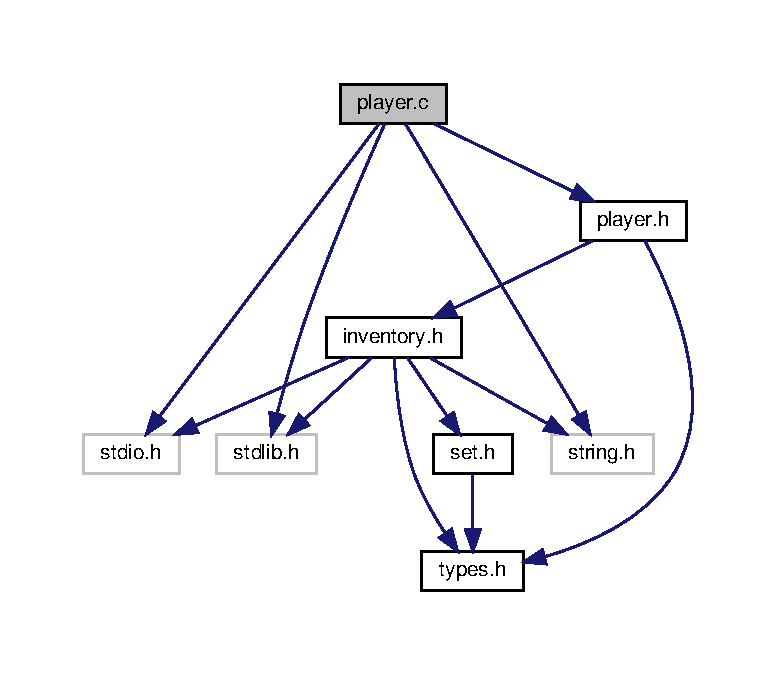
\includegraphics[width=350pt]{player_8c__incl}
\end{center}
\end{figure}
\subsection*{Classes}
\begin{DoxyCompactItemize}
\item 
struct \hyperlink{struct__Player}{\+\_\+\+Player}
\end{DoxyCompactItemize}
\subsection*{Functions}
\begin{DoxyCompactItemize}
\item 
\hyperlink{player_8h_af30e2030635a69690f85e48bc6ef202f}{Player} $\ast$ \hyperlink{player_8c_a5e6b11365804f0ccebd2fac6d410369e}{player\+\_\+create} (int max\+\_\+obj)
\begin{DoxyCompactList}\small\item\em crea un jugador \end{DoxyCompactList}\item 
\hyperlink{types_8h_a32c27cc471df37f4fc818d65de0a56c4}{S\+T\+A\+T\+US} \hyperlink{player_8c_a68e324aa5064e27d0a2f38aafb6809ad}{player\+\_\+destroy} (\hyperlink{player_8h_af30e2030635a69690f85e48bc6ef202f}{Player} $\ast$player)
\begin{DoxyCompactList}\small\item\em destruye un jugador \end{DoxyCompactList}\item 
\hyperlink{types_8h_a32c27cc471df37f4fc818d65de0a56c4}{S\+T\+A\+T\+US} \hyperlink{player_8c_a6a30809f7775f5c2d3bef47d92769e59}{player\+\_\+set\+\_\+name} (\hyperlink{player_8h_af30e2030635a69690f85e48bc6ef202f}{Player} $\ast$player, char $\ast$name)
\begin{DoxyCompactList}\small\item\em cambia el nombre de un jugador \end{DoxyCompactList}\item 
\hyperlink{types_8h_a32c27cc471df37f4fc818d65de0a56c4}{S\+T\+A\+T\+US} \hyperlink{player_8c_a511658c8ff616308825ae86d4bae2dd2}{player\+\_\+set\+\_\+id} (\hyperlink{player_8h_af30e2030635a69690f85e48bc6ef202f}{Player} $\ast$player, \hyperlink{types_8h_a845e604fb28f7e3d97549da3448149d3}{Id} id)
\begin{DoxyCompactList}\small\item\em cambia el Id de un jugador \end{DoxyCompactList}\item 
\hyperlink{types_8h_a32c27cc471df37f4fc818d65de0a56c4}{S\+T\+A\+T\+US} \hyperlink{player_8c_acea7143b0c9933e4c6f2fe699526e6f9}{player\+\_\+set\+\_\+inventory} (\hyperlink{player_8h_af30e2030635a69690f85e48bc6ef202f}{Player} $\ast$player, \hyperlink{inventory_8h_a2253bf64ac4ce6a9c1d6f39c0b0d32a3}{Inventory} $\ast$bag)
\begin{DoxyCompactList}\small\item\em cambia el inventario de un jugador \end{DoxyCompactList}\item 
\hyperlink{types_8h_a32c27cc471df37f4fc818d65de0a56c4}{S\+T\+A\+T\+US} \hyperlink{player_8c_a280029f648f6d52747c95d81621b12d4}{player\+\_\+set\+\_\+space\+\_\+id} (\hyperlink{player_8h_af30e2030635a69690f85e48bc6ef202f}{Player} $\ast$player, \hyperlink{types_8h_a845e604fb28f7e3d97549da3448149d3}{Id} space\+\_\+id)
\begin{DoxyCompactList}\small\item\em cambia el Id de la posicion de un jugador \end{DoxyCompactList}\item 
char $\ast$ \hyperlink{player_8c_a260d3419c458edcdb3d2b5e9d4a867e8}{player\+\_\+get\+\_\+name} (\hyperlink{player_8h_af30e2030635a69690f85e48bc6ef202f}{Player} $\ast$player)
\begin{DoxyCompactList}\small\item\em devuelve el nombre de un jugador \end{DoxyCompactList}\item 
\hyperlink{types_8h_a845e604fb28f7e3d97549da3448149d3}{Id} \hyperlink{player_8c_af5a101ec91427951c5875569a8709956}{player\+\_\+get\+\_\+id} (\hyperlink{player_8h_af30e2030635a69690f85e48bc6ef202f}{Player} $\ast$player)
\begin{DoxyCompactList}\small\item\em devuelve el Id de un jugador \end{DoxyCompactList}\item 
\hyperlink{types_8h_a845e604fb28f7e3d97549da3448149d3}{Id} \hyperlink{player_8c_acb8bca0eada9e103693473a53dcf7569}{player\+\_\+get\+\_\+space\+\_\+id} (\hyperlink{player_8h_af30e2030635a69690f85e48bc6ef202f}{Player} $\ast$player)
\begin{DoxyCompactList}\small\item\em devuelve el Id de la posicion de un jugador \end{DoxyCompactList}\item 
\hyperlink{inventory_8h_a2253bf64ac4ce6a9c1d6f39c0b0d32a3}{Inventory} $\ast$ \hyperlink{player_8c_a270da6469a85e0c2b7f9f4088d290051}{player\+\_\+get\+\_\+inventory} (\hyperlink{player_8h_af30e2030635a69690f85e48bc6ef202f}{Player} $\ast$player)
\begin{DoxyCompactList}\small\item\em devuelve el inventario de un jugador \end{DoxyCompactList}\item 
\hyperlink{types_8h_a32c27cc471df37f4fc818d65de0a56c4}{S\+T\+A\+T\+US} \hyperlink{player_8c_a433ca0333cf23c1e213e3b4ffe654654}{player\+\_\+drop\+\_\+object} (\hyperlink{player_8h_af30e2030635a69690f85e48bc6ef202f}{Player} $\ast$player, \hyperlink{types_8h_a845e604fb28f7e3d97549da3448149d3}{Id} id)
\begin{DoxyCompactList}\small\item\em suelta un objeto que tiene el jugador \end{DoxyCompactList}\item 
\hyperlink{types_8h_a32c27cc471df37f4fc818d65de0a56c4}{S\+T\+A\+T\+US} \hyperlink{player_8c_a672d857a4a76b51c19f8b916175c92da}{player\+\_\+pick\+\_\+object} (\hyperlink{player_8h_af30e2030635a69690f85e48bc6ef202f}{Player} $\ast$player, \hyperlink{types_8h_a845e604fb28f7e3d97549da3448149d3}{Id} id)
\begin{DoxyCompactList}\small\item\em el jugador coge un objeto \end{DoxyCompactList}\item 
\hyperlink{types_8h_a3e5b8192e7d9ffaf3542f1210aec18dd}{B\+O\+OL} \hyperlink{player_8c_ad5a08e5ca32270d87cf1494099a1cb25}{player\+\_\+has\+\_\+object} (\hyperlink{player_8h_af30e2030635a69690f85e48bc6ef202f}{Player} $\ast$player, \hyperlink{types_8h_a845e604fb28f7e3d97549da3448149d3}{Id} id)
\begin{DoxyCompactList}\small\item\em comprueba si un jugador tiene un objeto \end{DoxyCompactList}\item 
\hyperlink{types_8h_a3e5b8192e7d9ffaf3542f1210aec18dd}{B\+O\+OL} \hyperlink{player_8c_a843c6afd4ecaafd61e85ab5f866be7e1}{player\+\_\+bag\+\_\+is\+\_\+full} (\hyperlink{player_8h_af30e2030635a69690f85e48bc6ef202f}{Player} $\ast$player)
\begin{DoxyCompactList}\small\item\em el jugador tiene el inventario lleno \end{DoxyCompactList}\item 
int \hyperlink{player_8c_a8d1daf5ac3f9445145d4ec45e70f5940}{player\+\_\+print} (F\+I\+LE $\ast$f, \hyperlink{player_8h_af30e2030635a69690f85e48bc6ef202f}{Player} $\ast$player)
\begin{DoxyCompactList}\small\item\em imprime el jugador \end{DoxyCompactList}\end{DoxyCompactItemize}


\subsection{Detailed Description}
En este fichero implementamos las funciones del jugador. 

\begin{DoxyAuthor}{Author}
Manuel Suarez, Saul Almazán, Álvaro Becerra, Rodrigo Lardiés 
\end{DoxyAuthor}
\begin{DoxyVersion}{Version}
1.\+0 
\end{DoxyVersion}
\begin{DoxyDate}{Date}
20/10/2018 
\end{DoxyDate}


\subsection{Function Documentation}
\mbox{\Hypertarget{player_8c_a843c6afd4ecaafd61e85ab5f866be7e1}\label{player_8c_a843c6afd4ecaafd61e85ab5f866be7e1}} 
\index{player.\+c@{player.\+c}!player\+\_\+bag\+\_\+is\+\_\+full@{player\+\_\+bag\+\_\+is\+\_\+full}}
\index{player\+\_\+bag\+\_\+is\+\_\+full@{player\+\_\+bag\+\_\+is\+\_\+full}!player.\+c@{player.\+c}}
\subsubsection{\texorpdfstring{player\+\_\+bag\+\_\+is\+\_\+full()}{player\_bag\_is\_full()}}
{\footnotesize\ttfamily \hyperlink{types_8h_a3e5b8192e7d9ffaf3542f1210aec18dd}{B\+O\+OL} player\+\_\+bag\+\_\+is\+\_\+full (\begin{DoxyParamCaption}\item[{\hyperlink{player_8h_af30e2030635a69690f85e48bc6ef202f}{Player} $\ast$}]{player }\end{DoxyParamCaption})}



el jugador tiene el inventario lleno 

\begin{DoxyAuthor}{Author}
Manuel Suarez, Saul Almazán, Álvaro Becerra, Rodrigo Lardiés 
\end{DoxyAuthor}
\begin{DoxyDate}{Date}
20/10/2018 
\end{DoxyDate}

\begin{DoxyParams}{Parameters}
{\em player} & (jugador a usar) \\
\hline
\end{DoxyParams}
\begin{DoxyReturn}{Returns}
B\+O\+OL (T\+R\+UE si el jugador tiene el inventario lleno o F\+A\+L\+SE de lo contrario) 
\end{DoxyReturn}
\mbox{\Hypertarget{player_8c_a5e6b11365804f0ccebd2fac6d410369e}\label{player_8c_a5e6b11365804f0ccebd2fac6d410369e}} 
\index{player.\+c@{player.\+c}!player\+\_\+create@{player\+\_\+create}}
\index{player\+\_\+create@{player\+\_\+create}!player.\+c@{player.\+c}}
\subsubsection{\texorpdfstring{player\+\_\+create()}{player\_create()}}
{\footnotesize\ttfamily \hyperlink{player_8h_af30e2030635a69690f85e48bc6ef202f}{Player}$\ast$ player\+\_\+create (\begin{DoxyParamCaption}\item[{int}]{max\+\_\+obj }\end{DoxyParamCaption})}



crea un jugador 

\begin{DoxyAuthor}{Author}
Manuel Suarez, Saul Almazán, Álvaro Becerra, Rodrigo Lardiés 
\end{DoxyAuthor}
\begin{DoxyDate}{Date}
20/10/201 
\end{DoxyDate}

\begin{DoxyParams}{Parameters}
{\em max\+\_\+obj} & (numero maximo de objetos de un jugador) \\
\hline
\end{DoxyParams}
\begin{DoxyReturn}{Returns}
Player$\ast$ (El jugador que crea) 
\end{DoxyReturn}
\mbox{\Hypertarget{player_8c_a68e324aa5064e27d0a2f38aafb6809ad}\label{player_8c_a68e324aa5064e27d0a2f38aafb6809ad}} 
\index{player.\+c@{player.\+c}!player\+\_\+destroy@{player\+\_\+destroy}}
\index{player\+\_\+destroy@{player\+\_\+destroy}!player.\+c@{player.\+c}}
\subsubsection{\texorpdfstring{player\+\_\+destroy()}{player\_destroy()}}
{\footnotesize\ttfamily \hyperlink{types_8h_a32c27cc471df37f4fc818d65de0a56c4}{S\+T\+A\+T\+US} player\+\_\+destroy (\begin{DoxyParamCaption}\item[{\hyperlink{player_8h_af30e2030635a69690f85e48bc6ef202f}{Player} $\ast$}]{player }\end{DoxyParamCaption})}



destruye un jugador 

\begin{DoxyAuthor}{Author}
Manuel Suarez, Saul Almazán, Álvaro Becerra, Rodrigo Lardiés 
\end{DoxyAuthor}
\begin{DoxyDate}{Date}
20/10/2018 
\end{DoxyDate}

\begin{DoxyParams}{Parameters}
{\em player} & (jugador a destruir) \\
\hline
\end{DoxyParams}
\begin{DoxyReturn}{Returns}
S\+T\+A\+T\+US (OK si se realiza con exito o E\+R\+R\+OR de lo contrario) 
\end{DoxyReturn}
\mbox{\Hypertarget{player_8c_a433ca0333cf23c1e213e3b4ffe654654}\label{player_8c_a433ca0333cf23c1e213e3b4ffe654654}} 
\index{player.\+c@{player.\+c}!player\+\_\+drop\+\_\+object@{player\+\_\+drop\+\_\+object}}
\index{player\+\_\+drop\+\_\+object@{player\+\_\+drop\+\_\+object}!player.\+c@{player.\+c}}
\subsubsection{\texorpdfstring{player\+\_\+drop\+\_\+object()}{player\_drop\_object()}}
{\footnotesize\ttfamily \hyperlink{types_8h_a32c27cc471df37f4fc818d65de0a56c4}{S\+T\+A\+T\+US} player\+\_\+drop\+\_\+object (\begin{DoxyParamCaption}\item[{\hyperlink{player_8h_af30e2030635a69690f85e48bc6ef202f}{Player} $\ast$}]{player,  }\item[{\hyperlink{types_8h_a845e604fb28f7e3d97549da3448149d3}{Id}}]{id }\end{DoxyParamCaption})}



suelta un objeto que tiene el jugador 

\begin{DoxyAuthor}{Author}
Manuel Suarez, Saul Almazán, Álvaro Becerra, Rodrigo Lardiés 
\end{DoxyAuthor}
\begin{DoxyDate}{Date}
20/10/2018 
\end{DoxyDate}

\begin{DoxyParams}{Parameters}
{\em player} & (jugador a usar) \\
\hline
{\em id} & (Id del objeto a soltar) \\
\hline
\end{DoxyParams}
\begin{DoxyReturn}{Returns}
S\+T\+A\+T\+US (OK si se realiza con exito o E\+R\+R\+OR de lo contrario) 
\end{DoxyReturn}
\mbox{\Hypertarget{player_8c_af5a101ec91427951c5875569a8709956}\label{player_8c_af5a101ec91427951c5875569a8709956}} 
\index{player.\+c@{player.\+c}!player\+\_\+get\+\_\+id@{player\+\_\+get\+\_\+id}}
\index{player\+\_\+get\+\_\+id@{player\+\_\+get\+\_\+id}!player.\+c@{player.\+c}}
\subsubsection{\texorpdfstring{player\+\_\+get\+\_\+id()}{player\_get\_id()}}
{\footnotesize\ttfamily \hyperlink{types_8h_a845e604fb28f7e3d97549da3448149d3}{Id} player\+\_\+get\+\_\+id (\begin{DoxyParamCaption}\item[{\hyperlink{player_8h_af30e2030635a69690f85e48bc6ef202f}{Player} $\ast$}]{player }\end{DoxyParamCaption})}



devuelve el Id de un jugador 

\begin{DoxyAuthor}{Author}
Manuel Suarez, Saul Almazán, Álvaro Becerra, Rodrigo Lardiés 
\end{DoxyAuthor}
\begin{DoxyDate}{Date}
20/10/2018 
\end{DoxyDate}

\begin{DoxyParams}{Parameters}
{\em player} & (jugador a usar) \\
\hline
\end{DoxyParams}
\begin{DoxyReturn}{Returns}
Id (Devuelve el Id del jugador) 
\end{DoxyReturn}
\mbox{\Hypertarget{player_8c_a270da6469a85e0c2b7f9f4088d290051}\label{player_8c_a270da6469a85e0c2b7f9f4088d290051}} 
\index{player.\+c@{player.\+c}!player\+\_\+get\+\_\+inventory@{player\+\_\+get\+\_\+inventory}}
\index{player\+\_\+get\+\_\+inventory@{player\+\_\+get\+\_\+inventory}!player.\+c@{player.\+c}}
\subsubsection{\texorpdfstring{player\+\_\+get\+\_\+inventory()}{player\_get\_inventory()}}
{\footnotesize\ttfamily \hyperlink{inventory_8h_a2253bf64ac4ce6a9c1d6f39c0b0d32a3}{Inventory}$\ast$ player\+\_\+get\+\_\+inventory (\begin{DoxyParamCaption}\item[{\hyperlink{player_8h_af30e2030635a69690f85e48bc6ef202f}{Player} $\ast$}]{player }\end{DoxyParamCaption})}



devuelve el inventario de un jugador 

\begin{DoxyAuthor}{Author}
Manuel Suarez, Saul Almazán, Álvaro Becerra, Rodrigo Lardiés 
\end{DoxyAuthor}
\begin{DoxyDate}{Date}
20/10/2018 
\end{DoxyDate}

\begin{DoxyParams}{Parameters}
{\em player} & (jugador a usar) \\
\hline
\end{DoxyParams}
\begin{DoxyReturn}{Returns}
Inventory$\ast$ (Devuelve el inventario del jugador) 
\end{DoxyReturn}
\mbox{\Hypertarget{player_8c_a260d3419c458edcdb3d2b5e9d4a867e8}\label{player_8c_a260d3419c458edcdb3d2b5e9d4a867e8}} 
\index{player.\+c@{player.\+c}!player\+\_\+get\+\_\+name@{player\+\_\+get\+\_\+name}}
\index{player\+\_\+get\+\_\+name@{player\+\_\+get\+\_\+name}!player.\+c@{player.\+c}}
\subsubsection{\texorpdfstring{player\+\_\+get\+\_\+name()}{player\_get\_name()}}
{\footnotesize\ttfamily char$\ast$ player\+\_\+get\+\_\+name (\begin{DoxyParamCaption}\item[{\hyperlink{player_8h_af30e2030635a69690f85e48bc6ef202f}{Player} $\ast$}]{player }\end{DoxyParamCaption})}



devuelve el nombre de un jugador 

\begin{DoxyAuthor}{Author}
Manuel Suarez, Saul Almazán, Álvaro Becerra, Rodrigo Lardiés 
\end{DoxyAuthor}
\begin{DoxyDate}{Date}
20/10/2018 
\end{DoxyDate}

\begin{DoxyParams}{Parameters}
{\em player} & (jugador a usar) \\
\hline
\end{DoxyParams}
\begin{DoxyReturn}{Returns}
char$\ast$ (Devuelve el nombre del objeto) 
\end{DoxyReturn}
\mbox{\Hypertarget{player_8c_acb8bca0eada9e103693473a53dcf7569}\label{player_8c_acb8bca0eada9e103693473a53dcf7569}} 
\index{player.\+c@{player.\+c}!player\+\_\+get\+\_\+space\+\_\+id@{player\+\_\+get\+\_\+space\+\_\+id}}
\index{player\+\_\+get\+\_\+space\+\_\+id@{player\+\_\+get\+\_\+space\+\_\+id}!player.\+c@{player.\+c}}
\subsubsection{\texorpdfstring{player\+\_\+get\+\_\+space\+\_\+id()}{player\_get\_space\_id()}}
{\footnotesize\ttfamily \hyperlink{types_8h_a845e604fb28f7e3d97549da3448149d3}{Id} player\+\_\+get\+\_\+space\+\_\+id (\begin{DoxyParamCaption}\item[{\hyperlink{player_8h_af30e2030635a69690f85e48bc6ef202f}{Player} $\ast$}]{player }\end{DoxyParamCaption})}



devuelve el Id de la posicion de un jugador 

\begin{DoxyAuthor}{Author}
Manuel Suarez, Saul Almazán, Álvaro Becerra, Rodrigo Lardiés 
\end{DoxyAuthor}
\begin{DoxyDate}{Date}
20/10/2018 
\end{DoxyDate}

\begin{DoxyParams}{Parameters}
{\em player} & (jugador a usar) \\
\hline
\end{DoxyParams}
\begin{DoxyReturn}{Returns}
Id (Devuelve el Id de la posicion del jugador) 
\end{DoxyReturn}
\mbox{\Hypertarget{player_8c_ad5a08e5ca32270d87cf1494099a1cb25}\label{player_8c_ad5a08e5ca32270d87cf1494099a1cb25}} 
\index{player.\+c@{player.\+c}!player\+\_\+has\+\_\+object@{player\+\_\+has\+\_\+object}}
\index{player\+\_\+has\+\_\+object@{player\+\_\+has\+\_\+object}!player.\+c@{player.\+c}}
\subsubsection{\texorpdfstring{player\+\_\+has\+\_\+object()}{player\_has\_object()}}
{\footnotesize\ttfamily \hyperlink{types_8h_a3e5b8192e7d9ffaf3542f1210aec18dd}{B\+O\+OL} player\+\_\+has\+\_\+object (\begin{DoxyParamCaption}\item[{\hyperlink{player_8h_af30e2030635a69690f85e48bc6ef202f}{Player} $\ast$}]{player,  }\item[{\hyperlink{types_8h_a845e604fb28f7e3d97549da3448149d3}{Id}}]{id }\end{DoxyParamCaption})}



comprueba si un jugador tiene un objeto 

\begin{DoxyAuthor}{Author}
Manuel Suarez, Saul Almazán, Álvaro Becerra, Rodrigo Lardiés 
\end{DoxyAuthor}
\begin{DoxyDate}{Date}
20/10/2018 
\end{DoxyDate}

\begin{DoxyParams}{Parameters}
{\em player} & (jugador a usar) \\
\hline
{\em id} & (Id del objeto a comprobar) \\
\hline
\end{DoxyParams}
\begin{DoxyReturn}{Returns}
B\+O\+OL (T\+R\+UE si el jugador tiene el objeto o F\+A\+L\+SE de lo contrario) 
\end{DoxyReturn}
\mbox{\Hypertarget{player_8c_a672d857a4a76b51c19f8b916175c92da}\label{player_8c_a672d857a4a76b51c19f8b916175c92da}} 
\index{player.\+c@{player.\+c}!player\+\_\+pick\+\_\+object@{player\+\_\+pick\+\_\+object}}
\index{player\+\_\+pick\+\_\+object@{player\+\_\+pick\+\_\+object}!player.\+c@{player.\+c}}
\subsubsection{\texorpdfstring{player\+\_\+pick\+\_\+object()}{player\_pick\_object()}}
{\footnotesize\ttfamily \hyperlink{types_8h_a32c27cc471df37f4fc818d65de0a56c4}{S\+T\+A\+T\+US} player\+\_\+pick\+\_\+object (\begin{DoxyParamCaption}\item[{\hyperlink{player_8h_af30e2030635a69690f85e48bc6ef202f}{Player} $\ast$}]{player,  }\item[{\hyperlink{types_8h_a845e604fb28f7e3d97549da3448149d3}{Id}}]{id }\end{DoxyParamCaption})}



el jugador coge un objeto 

\begin{DoxyAuthor}{Author}
Manuel Suarez, Saul Almazán, Álvaro Becerra, Rodrigo Lardiés 
\end{DoxyAuthor}
\begin{DoxyDate}{Date}
20/10/2018 
\end{DoxyDate}

\begin{DoxyParams}{Parameters}
{\em player} & (jugador a usar) \\
\hline
{\em id} & (Id del objeto a coger) \\
\hline
\end{DoxyParams}
\begin{DoxyReturn}{Returns}
S\+T\+A\+T\+US (OK si se realiza con exito o E\+R\+R\+OR de lo contrario) 
\end{DoxyReturn}
\mbox{\Hypertarget{player_8c_a8d1daf5ac3f9445145d4ec45e70f5940}\label{player_8c_a8d1daf5ac3f9445145d4ec45e70f5940}} 
\index{player.\+c@{player.\+c}!player\+\_\+print@{player\+\_\+print}}
\index{player\+\_\+print@{player\+\_\+print}!player.\+c@{player.\+c}}
\subsubsection{\texorpdfstring{player\+\_\+print()}{player\_print()}}
{\footnotesize\ttfamily int player\+\_\+print (\begin{DoxyParamCaption}\item[{F\+I\+LE $\ast$}]{f,  }\item[{\hyperlink{player_8h_af30e2030635a69690f85e48bc6ef202f}{Player} $\ast$}]{player }\end{DoxyParamCaption})}



imprime el jugador 

\begin{DoxyAuthor}{Author}
Manuel Suarez, Saul Almazán, Álvaro Becerra, Rodrigo Lardiés 
\end{DoxyAuthor}
\begin{DoxyDate}{Date}
20/10/2018 
\end{DoxyDate}

\begin{DoxyParams}{Parameters}
{\em player} & (jugador a usar) \\
\hline
{\em f} & (donde se va a imprimir) \\
\hline
\end{DoxyParams}
\begin{DoxyReturn}{Returns}
int (-\/1 si hay algun error) 
\end{DoxyReturn}
\mbox{\Hypertarget{player_8c_a511658c8ff616308825ae86d4bae2dd2}\label{player_8c_a511658c8ff616308825ae86d4bae2dd2}} 
\index{player.\+c@{player.\+c}!player\+\_\+set\+\_\+id@{player\+\_\+set\+\_\+id}}
\index{player\+\_\+set\+\_\+id@{player\+\_\+set\+\_\+id}!player.\+c@{player.\+c}}
\subsubsection{\texorpdfstring{player\+\_\+set\+\_\+id()}{player\_set\_id()}}
{\footnotesize\ttfamily \hyperlink{types_8h_a32c27cc471df37f4fc818d65de0a56c4}{S\+T\+A\+T\+US} player\+\_\+set\+\_\+id (\begin{DoxyParamCaption}\item[{\hyperlink{player_8h_af30e2030635a69690f85e48bc6ef202f}{Player} $\ast$}]{player,  }\item[{\hyperlink{types_8h_a845e604fb28f7e3d97549da3448149d3}{Id}}]{id }\end{DoxyParamCaption})}



cambia el Id de un jugador 

\begin{DoxyAuthor}{Author}
Manuel Suarez, Saul Almazán, Álvaro Becerra, Rodrigo Lardiés 
\end{DoxyAuthor}
\begin{DoxyDate}{Date}
20/10/2018 
\end{DoxyDate}

\begin{DoxyParams}{Parameters}
{\em player} & (jugador a modificar) \\
\hline
{\em id} & (nuevo Id) \\
\hline
\end{DoxyParams}
\begin{DoxyReturn}{Returns}
S\+T\+A\+T\+US (OK si se realiza con exito o E\+R\+R\+OR de lo contrario) 
\end{DoxyReturn}
\mbox{\Hypertarget{player_8c_acea7143b0c9933e4c6f2fe699526e6f9}\label{player_8c_acea7143b0c9933e4c6f2fe699526e6f9}} 
\index{player.\+c@{player.\+c}!player\+\_\+set\+\_\+inventory@{player\+\_\+set\+\_\+inventory}}
\index{player\+\_\+set\+\_\+inventory@{player\+\_\+set\+\_\+inventory}!player.\+c@{player.\+c}}
\subsubsection{\texorpdfstring{player\+\_\+set\+\_\+inventory()}{player\_set\_inventory()}}
{\footnotesize\ttfamily \hyperlink{types_8h_a32c27cc471df37f4fc818d65de0a56c4}{S\+T\+A\+T\+US} player\+\_\+set\+\_\+inventory (\begin{DoxyParamCaption}\item[{\hyperlink{player_8h_af30e2030635a69690f85e48bc6ef202f}{Player} $\ast$}]{player,  }\item[{\hyperlink{inventory_8h_a2253bf64ac4ce6a9c1d6f39c0b0d32a3}{Inventory} $\ast$}]{bag }\end{DoxyParamCaption})}



cambia el inventario de un jugador 

\begin{DoxyAuthor}{Author}
Manuel Suarez, Saul Almazán, Álvaro Becerra, Rodrigo Lardiés 
\end{DoxyAuthor}
\begin{DoxyDate}{Date}
20/10/2018 
\end{DoxyDate}

\begin{DoxyParams}{Parameters}
{\em player} & (jugador a modificar) \\
\hline
{\em bag} & (nuevo inventario) \\
\hline
\end{DoxyParams}
\begin{DoxyReturn}{Returns}
S\+T\+A\+T\+US (OK si se realiza con exito o E\+R\+R\+OR de lo contrario) 
\end{DoxyReturn}
\mbox{\Hypertarget{player_8c_a6a30809f7775f5c2d3bef47d92769e59}\label{player_8c_a6a30809f7775f5c2d3bef47d92769e59}} 
\index{player.\+c@{player.\+c}!player\+\_\+set\+\_\+name@{player\+\_\+set\+\_\+name}}
\index{player\+\_\+set\+\_\+name@{player\+\_\+set\+\_\+name}!player.\+c@{player.\+c}}
\subsubsection{\texorpdfstring{player\+\_\+set\+\_\+name()}{player\_set\_name()}}
{\footnotesize\ttfamily \hyperlink{types_8h_a32c27cc471df37f4fc818d65de0a56c4}{S\+T\+A\+T\+US} player\+\_\+set\+\_\+name (\begin{DoxyParamCaption}\item[{\hyperlink{player_8h_af30e2030635a69690f85e48bc6ef202f}{Player} $\ast$}]{player,  }\item[{char $\ast$}]{name }\end{DoxyParamCaption})}



cambia el nombre de un jugador 

\begin{DoxyAuthor}{Author}
Manuel Suarez, Saul Almazán, Álvaro Becerra, Rodrigo Lardiés 
\end{DoxyAuthor}
\begin{DoxyDate}{Date}
20/10/2018 
\end{DoxyDate}

\begin{DoxyParams}{Parameters}
{\em player} & (jugador a modificar) \\
\hline
{\em name} & (nuevo nombre) \\
\hline
\end{DoxyParams}
\begin{DoxyReturn}{Returns}
S\+T\+A\+T\+US (OK si se realiza con exito o E\+R\+R\+OR de lo contrario) 
\end{DoxyReturn}
\mbox{\Hypertarget{player_8c_a280029f648f6d52747c95d81621b12d4}\label{player_8c_a280029f648f6d52747c95d81621b12d4}} 
\index{player.\+c@{player.\+c}!player\+\_\+set\+\_\+space\+\_\+id@{player\+\_\+set\+\_\+space\+\_\+id}}
\index{player\+\_\+set\+\_\+space\+\_\+id@{player\+\_\+set\+\_\+space\+\_\+id}!player.\+c@{player.\+c}}
\subsubsection{\texorpdfstring{player\+\_\+set\+\_\+space\+\_\+id()}{player\_set\_space\_id()}}
{\footnotesize\ttfamily \hyperlink{types_8h_a32c27cc471df37f4fc818d65de0a56c4}{S\+T\+A\+T\+US} player\+\_\+set\+\_\+space\+\_\+id (\begin{DoxyParamCaption}\item[{\hyperlink{player_8h_af30e2030635a69690f85e48bc6ef202f}{Player} $\ast$}]{player,  }\item[{\hyperlink{types_8h_a845e604fb28f7e3d97549da3448149d3}{Id}}]{space\+\_\+id }\end{DoxyParamCaption})}



cambia el Id de la posicion de un jugador 

\begin{DoxyAuthor}{Author}
Manuel Suarez, Saul Almazán, Álvaro Becerra, Rodrigo Lardiés 
\end{DoxyAuthor}
\begin{DoxyDate}{Date}
20/10/2018 
\end{DoxyDate}

\begin{DoxyParams}{Parameters}
{\em player} & (jugador a modificar) \\
\hline
{\em space\+\_\+id} & (nuevo Id de posicion) \\
\hline
\end{DoxyParams}
\begin{DoxyReturn}{Returns}
S\+T\+A\+T\+US (OK si se realiza con exito o E\+R\+R\+OR de lo contrario) 
\end{DoxyReturn}

\hypertarget{player__test_8c}{}\section{src/player\+\_\+test.c File Reference}
\label{player__test_8c}\index{src/player\+\_\+test.\+c@{src/player\+\_\+test.\+c}}


Prueba del modulo player.  


{\ttfamily \#include $<$stdio.\+h$>$}\newline
{\ttfamily \#include $<$stdlib.\+h$>$}\newline
{\ttfamily \#include $<$string.\+h$>$}\newline
{\ttfamily \#include \char`\"{}player.\+h\char`\"{}}\newline
{\ttfamily \#include \char`\"{}player\+\_\+test.\+h\char`\"{}}\newline
{\ttfamily \#include \char`\"{}test.\+h\char`\"{}}\newline
Include dependency graph for player\+\_\+test.\+c\+:
% FIG 0
\subsection*{Macros}
\begin{DoxyCompactItemize}
\item 
\#define \hyperlink{player__test_8c_a2a77d2f2c5b698c69c19e1f8782bf709}{M\+A\+X\+\_\+\+T\+E\+S\+TS}~23
\end{DoxyCompactItemize}
\subsection*{Functions}
\begin{DoxyCompactItemize}
\item 
int \hyperlink{player__test_8c_a3c04138a5bfe5d72780bb7e82a18e627}{main} (int argc, char $\ast$$\ast$argv)
\begin{DoxyCompactList}\small\item\em Funcion principal de pruebas para el modulo player. \end{DoxyCompactList}\item 
void \hyperlink{player__test_8c_ab29768452373e16bb6aaa1f7998f62fb}{test1\+\_\+player\+\_\+create} ()
\item 
void \hyperlink{player__test_8c_a4f6eca5f9d8c08d2a7fc70c209ecf854}{test2\+\_\+player\+\_\+create} ()
\item 
void \hyperlink{player__test_8c_a9d87c09e6af910d695265e3fd77ae3a2}{test1\+\_\+player\+\_\+set\+\_\+name} ()
\item 
void \hyperlink{player__test_8c_a6e7ce8ff791f4bf63749df647a44263f}{test2\+\_\+player\+\_\+set\+\_\+name} ()
\item 
void \hyperlink{player__test_8c_a447ebbb4ba2206abeaf4b60200e312da}{test3\+\_\+player\+\_\+set\+\_\+name} ()
\item 
void \hyperlink{player__test_8c_a64fa15a235953bea694236b9d7841cbc}{test1\+\_\+player\+\_\+set\+\_\+id} ()
\item 
void \hyperlink{player__test_8c_a3695e0896bc3d770290e6a691fa212f7}{test2\+\_\+player\+\_\+set\+\_\+id} ()
\item 
void \hyperlink{player__test_8c_ae6151348bf59b8e4e4ae4c2204ac3e36}{test1\+\_\+player\+\_\+set\+\_\+space\+\_\+id} ()
\item 
void \hyperlink{player__test_8c_a7c56960ab99cd14862dda28c157339e3}{test2\+\_\+player\+\_\+set\+\_\+space\+\_\+id} ()
\item 
void \hyperlink{player__test_8c_a94068667d8faa66a4ad293dd2c60f2ef}{test1\+\_\+player\+\_\+get\+\_\+name} ()
\item 
void \hyperlink{player__test_8c_a3aa908fd360b74e7786422260e8e16a0}{test2\+\_\+player\+\_\+get\+\_\+name} ()
\item 
void \hyperlink{player__test_8c_a790a75dc179c00c60c784d3e34c0e5aa}{test1\+\_\+player\+\_\+get\+\_\+id} ()
\item 
void \hyperlink{player__test_8c_a9fa80f0c0e46b45eb9f1685b102a5826}{test2\+\_\+player\+\_\+get\+\_\+id} ()
\item 
void \hyperlink{player__test_8c_ad3352b068fb75cc3763573f0125431f0}{test1\+\_\+player\+\_\+get\+\_\+space\+\_\+id} ()
\item 
void \hyperlink{player__test_8c_a4f9a990391473b00c42c6c285ec7ee37}{test2\+\_\+player\+\_\+get\+\_\+space\+\_\+id} ()
\item 
void \hyperlink{player__test_8c_a914b9b6ed41aa24340919e3dc72d6903}{test1\+\_\+player\+\_\+drop\+\_\+object} ()
\item 
void \hyperlink{player__test_8c_a2b1d4db679c85da5bd43347c583112f4}{test2\+\_\+player\+\_\+drop\+\_\+object} ()
\item 
void \hyperlink{player__test_8c_afac1cd8f32bcda203e7990c6bb9497a7}{test1\+\_\+player\+\_\+pick\+\_\+object} ()
\item 
void \hyperlink{player__test_8c_aab964f085041375e79d42d314c5a2202}{test2\+\_\+player\+\_\+pick\+\_\+object} ()
\item 
void \hyperlink{player__test_8c_abedc0e75ebffb4e7224f5e5ac0ee3055}{test1\+\_\+player\+\_\+has\+\_\+object} ()
\item 
void \hyperlink{player__test_8c_ae8953d45d8f555a930dbc8aba101d399}{test2\+\_\+player\+\_\+has\+\_\+object} ()
\item 
void \hyperlink{player__test_8c_acc5358622f284c28d03126605a3c8ad0}{test1\+\_\+player\+\_\+bag\+\_\+is\+\_\+full} ()
\item 
void \hyperlink{player__test_8c_aac711c53eb08f5e0d6966d80ede4f7ed}{test2\+\_\+player\+\_\+bag\+\_\+is\+\_\+full} ()
\end{DoxyCompactItemize}


\subsection{Detailed Description}
Prueba del modulo player. 

\begin{DoxyAuthor}{Author}
Manuel Suarez, Saul Almazán, �?lvaro Becerra, Rodrigo Lardiés 
\end{DoxyAuthor}
\begin{DoxyVersion}{Version}
1.\+0 
\end{DoxyVersion}
\begin{DoxyDate}{Date}
12-\/11-\/2018 
\end{DoxyDate}


\subsection{Macro Definition Documentation}
\mbox{\Hypertarget{player__test_8c_a2a77d2f2c5b698c69c19e1f8782bf709}\label{player__test_8c_a2a77d2f2c5b698c69c19e1f8782bf709}} 
\index{player\+\_\+test.\+c@{player\+\_\+test.\+c}!M\+A\+X\+\_\+\+T\+E\+S\+TS@{M\+A\+X\+\_\+\+T\+E\+S\+TS}}
\index{M\+A\+X\+\_\+\+T\+E\+S\+TS@{M\+A\+X\+\_\+\+T\+E\+S\+TS}!player\+\_\+test.\+c@{player\+\_\+test.\+c}}
\subsubsection{\texorpdfstring{M\+A\+X\+\_\+\+T\+E\+S\+TS}{MAX\_TESTS}}
{\footnotesize\ttfamily \#define M\+A\+X\+\_\+\+T\+E\+S\+TS~23}

T\+A\+M\+\_\+\+T\+E\+S\+TS 

\subsection{Function Documentation}
\mbox{\Hypertarget{player__test_8c_a3c04138a5bfe5d72780bb7e82a18e627}\label{player__test_8c_a3c04138a5bfe5d72780bb7e82a18e627}} 
\index{player\+\_\+test.\+c@{player\+\_\+test.\+c}!main@{main}}
\index{main@{main}!player\+\_\+test.\+c@{player\+\_\+test.\+c}}
\subsubsection{\texorpdfstring{main()}{main()}}
{\footnotesize\ttfamily int main (\begin{DoxyParamCaption}\item[{int}]{argc,  }\item[{char $\ast$$\ast$}]{argv }\end{DoxyParamCaption})}



Funcion principal de pruebas para el modulo player. 

Dos modos de ejecucion\+: 1.-\/\+Si se ejecuta sin parametros se ejecutan todas las pruebas 2.-\/\+Si se ejecuta con un numero entre 1 y el numero de pruebas solo ejecuta la prueba indicada \mbox{\Hypertarget{player__test_8c_acc5358622f284c28d03126605a3c8ad0}\label{player__test_8c_acc5358622f284c28d03126605a3c8ad0}} 
\index{player\+\_\+test.\+c@{player\+\_\+test.\+c}!test1\+\_\+player\+\_\+bag\+\_\+is\+\_\+full@{test1\+\_\+player\+\_\+bag\+\_\+is\+\_\+full}}
\index{test1\+\_\+player\+\_\+bag\+\_\+is\+\_\+full@{test1\+\_\+player\+\_\+bag\+\_\+is\+\_\+full}!player\+\_\+test.\+c@{player\+\_\+test.\+c}}
\subsubsection{\texorpdfstring{test1\+\_\+player\+\_\+bag\+\_\+is\+\_\+full()}{test1\_player\_bag\_is\_full()}}
{\footnotesize\ttfamily void test1\+\_\+player\+\_\+bag\+\_\+is\+\_\+full (\begin{DoxyParamCaption}{ }\end{DoxyParamCaption})}

\begin{DoxyRefDesc}{Test}
\item[\hyperlink{test__test000105}{Test}]Prueba la función para saber si la mochila de un jugador está llena \end{DoxyRefDesc}
\begin{DoxyPrecond}{Precondition}
Jugador con una mochila para más de un objeto 
\end{DoxyPrecond}
\begin{DoxyPostcond}{Postcondition}
La salida debe ser F\+A\+L\+SE 
\end{DoxyPostcond}
\mbox{\Hypertarget{player__test_8c_ab29768452373e16bb6aaa1f7998f62fb}\label{player__test_8c_ab29768452373e16bb6aaa1f7998f62fb}} 
\index{player\+\_\+test.\+c@{player\+\_\+test.\+c}!test1\+\_\+player\+\_\+create@{test1\+\_\+player\+\_\+create}}
\index{test1\+\_\+player\+\_\+create@{test1\+\_\+player\+\_\+create}!player\+\_\+test.\+c@{player\+\_\+test.\+c}}
\subsubsection{\texorpdfstring{test1\+\_\+player\+\_\+create()}{test1\_player\_create()}}
{\footnotesize\ttfamily void test1\+\_\+player\+\_\+create (\begin{DoxyParamCaption}{ }\end{DoxyParamCaption})}

\begin{DoxyRefDesc}{Test}
\item[\hyperlink{test__test000084}{Test}]Prueba la función de creación de un jugador \end{DoxyRefDesc}
\begin{DoxyPrecond}{Precondition}
Un numero de objetos como parámetro 
\end{DoxyPrecond}
\begin{DoxyPostcond}{Postcondition}
Un puntero no nulo al jugador creado 
\end{DoxyPostcond}
\mbox{\Hypertarget{player__test_8c_a914b9b6ed41aa24340919e3dc72d6903}\label{player__test_8c_a914b9b6ed41aa24340919e3dc72d6903}} 
\index{player\+\_\+test.\+c@{player\+\_\+test.\+c}!test1\+\_\+player\+\_\+drop\+\_\+object@{test1\+\_\+player\+\_\+drop\+\_\+object}}
\index{test1\+\_\+player\+\_\+drop\+\_\+object@{test1\+\_\+player\+\_\+drop\+\_\+object}!player\+\_\+test.\+c@{player\+\_\+test.\+c}}
\subsubsection{\texorpdfstring{test1\+\_\+player\+\_\+drop\+\_\+object()}{test1\_player\_drop\_object()}}
{\footnotesize\ttfamily void test1\+\_\+player\+\_\+drop\+\_\+object (\begin{DoxyParamCaption}{ }\end{DoxyParamCaption})}

\begin{DoxyRefDesc}{Test}
\item[\hyperlink{test__test000099}{Test}]Prueba la función para dejar un objeto de un jugador \end{DoxyRefDesc}
\begin{DoxyPrecond}{Precondition}
Jugador con un objeto 
\end{DoxyPrecond}
\begin{DoxyPostcond}{Postcondition}
La salida debe ser OK 
\end{DoxyPostcond}
\mbox{\Hypertarget{player__test_8c_a790a75dc179c00c60c784d3e34c0e5aa}\label{player__test_8c_a790a75dc179c00c60c784d3e34c0e5aa}} 
\index{player\+\_\+test.\+c@{player\+\_\+test.\+c}!test1\+\_\+player\+\_\+get\+\_\+id@{test1\+\_\+player\+\_\+get\+\_\+id}}
\index{test1\+\_\+player\+\_\+get\+\_\+id@{test1\+\_\+player\+\_\+get\+\_\+id}!player\+\_\+test.\+c@{player\+\_\+test.\+c}}
\subsubsection{\texorpdfstring{test1\+\_\+player\+\_\+get\+\_\+id()}{test1\_player\_get\_id()}}
{\footnotesize\ttfamily void test1\+\_\+player\+\_\+get\+\_\+id (\begin{DoxyParamCaption}{ }\end{DoxyParamCaption})}

\begin{DoxyRefDesc}{Test}
\item[\hyperlink{test__test000095}{Test}]Prueba la función para obtener el id de un jugador \end{DoxyRefDesc}
\begin{DoxyPrecond}{Precondition}
El jugador tiene un id establecido 
\end{DoxyPrecond}
\begin{DoxyPostcond}{Postcondition}
La salida debe ser id=1 
\end{DoxyPostcond}
\mbox{\Hypertarget{player__test_8c_a94068667d8faa66a4ad293dd2c60f2ef}\label{player__test_8c_a94068667d8faa66a4ad293dd2c60f2ef}} 
\index{player\+\_\+test.\+c@{player\+\_\+test.\+c}!test1\+\_\+player\+\_\+get\+\_\+name@{test1\+\_\+player\+\_\+get\+\_\+name}}
\index{test1\+\_\+player\+\_\+get\+\_\+name@{test1\+\_\+player\+\_\+get\+\_\+name}!player\+\_\+test.\+c@{player\+\_\+test.\+c}}
\subsubsection{\texorpdfstring{test1\+\_\+player\+\_\+get\+\_\+name()}{test1\_player\_get\_name()}}
{\footnotesize\ttfamily void test1\+\_\+player\+\_\+get\+\_\+name (\begin{DoxyParamCaption}{ }\end{DoxyParamCaption})}

\begin{DoxyRefDesc}{Test}
\item[\hyperlink{test__test000093}{Test}]Prueba la función para obtener el nombre de un jugador \end{DoxyRefDesc}
\begin{DoxyPrecond}{Precondition}
El jugador tiene un nombre establecido 
\end{DoxyPrecond}
\begin{DoxyPostcond}{Postcondition}
La salida debe ser una comparación de cadenas igual a 0 
\end{DoxyPostcond}
\mbox{\Hypertarget{player__test_8c_ad3352b068fb75cc3763573f0125431f0}\label{player__test_8c_ad3352b068fb75cc3763573f0125431f0}} 
\index{player\+\_\+test.\+c@{player\+\_\+test.\+c}!test1\+\_\+player\+\_\+get\+\_\+space\+\_\+id@{test1\+\_\+player\+\_\+get\+\_\+space\+\_\+id}}
\index{test1\+\_\+player\+\_\+get\+\_\+space\+\_\+id@{test1\+\_\+player\+\_\+get\+\_\+space\+\_\+id}!player\+\_\+test.\+c@{player\+\_\+test.\+c}}
\subsubsection{\texorpdfstring{test1\+\_\+player\+\_\+get\+\_\+space\+\_\+id()}{test1\_player\_get\_space\_id()}}
{\footnotesize\ttfamily void test1\+\_\+player\+\_\+get\+\_\+space\+\_\+id (\begin{DoxyParamCaption}{ }\end{DoxyParamCaption})}

\begin{DoxyRefDesc}{Test}
\item[\hyperlink{test__test000097}{Test}]Prueba la función para obtener el id de un espacio de un jugador \end{DoxyRefDesc}
\begin{DoxyPrecond}{Precondition}
El jugador tiene un id establecido 
\end{DoxyPrecond}
\begin{DoxyPostcond}{Postcondition}
La salida debe ser id=1 
\end{DoxyPostcond}
\mbox{\Hypertarget{player__test_8c_abedc0e75ebffb4e7224f5e5ac0ee3055}\label{player__test_8c_abedc0e75ebffb4e7224f5e5ac0ee3055}} 
\index{player\+\_\+test.\+c@{player\+\_\+test.\+c}!test1\+\_\+player\+\_\+has\+\_\+object@{test1\+\_\+player\+\_\+has\+\_\+object}}
\index{test1\+\_\+player\+\_\+has\+\_\+object@{test1\+\_\+player\+\_\+has\+\_\+object}!player\+\_\+test.\+c@{player\+\_\+test.\+c}}
\subsubsection{\texorpdfstring{test1\+\_\+player\+\_\+has\+\_\+object()}{test1\_player\_has\_object()}}
{\footnotesize\ttfamily void test1\+\_\+player\+\_\+has\+\_\+object (\begin{DoxyParamCaption}{ }\end{DoxyParamCaption})}

\begin{DoxyRefDesc}{Test}
\item[\hyperlink{test__test000103}{Test}]Prueba la función para saber si un jugador tiene un objeto \end{DoxyRefDesc}
\begin{DoxyPrecond}{Precondition}
Jugador con un objeto 
\end{DoxyPrecond}
\begin{DoxyPostcond}{Postcondition}
La salida debe ser T\+R\+UE 
\end{DoxyPostcond}
\mbox{\Hypertarget{player__test_8c_afac1cd8f32bcda203e7990c6bb9497a7}\label{player__test_8c_afac1cd8f32bcda203e7990c6bb9497a7}} 
\index{player\+\_\+test.\+c@{player\+\_\+test.\+c}!test1\+\_\+player\+\_\+pick\+\_\+object@{test1\+\_\+player\+\_\+pick\+\_\+object}}
\index{test1\+\_\+player\+\_\+pick\+\_\+object@{test1\+\_\+player\+\_\+pick\+\_\+object}!player\+\_\+test.\+c@{player\+\_\+test.\+c}}
\subsubsection{\texorpdfstring{test1\+\_\+player\+\_\+pick\+\_\+object()}{test1\_player\_pick\_object()}}
{\footnotesize\ttfamily void test1\+\_\+player\+\_\+pick\+\_\+object (\begin{DoxyParamCaption}{ }\end{DoxyParamCaption})}

\begin{DoxyRefDesc}{Test}
\item[\hyperlink{test__test000101}{Test}]Prueba la función para coger un objeto \end{DoxyRefDesc}
\begin{DoxyPrecond}{Precondition}
Jugador e id de un objeto 
\end{DoxyPrecond}
\begin{DoxyPostcond}{Postcondition}
La salida debe ser OK 
\end{DoxyPostcond}
\mbox{\Hypertarget{player__test_8c_a64fa15a235953bea694236b9d7841cbc}\label{player__test_8c_a64fa15a235953bea694236b9d7841cbc}} 
\index{player\+\_\+test.\+c@{player\+\_\+test.\+c}!test1\+\_\+player\+\_\+set\+\_\+id@{test1\+\_\+player\+\_\+set\+\_\+id}}
\index{test1\+\_\+player\+\_\+set\+\_\+id@{test1\+\_\+player\+\_\+set\+\_\+id}!player\+\_\+test.\+c@{player\+\_\+test.\+c}}
\subsubsection{\texorpdfstring{test1\+\_\+player\+\_\+set\+\_\+id()}{test1\_player\_set\_id()}}
{\footnotesize\ttfamily void test1\+\_\+player\+\_\+set\+\_\+id (\begin{DoxyParamCaption}{ }\end{DoxyParamCaption})}

\begin{DoxyRefDesc}{Test}
\item[\hyperlink{test__test000089}{Test}]Prueba la función para establecer el id de un jugador \end{DoxyRefDesc}
\begin{DoxyPrecond}{Precondition}
id que establecer al jugador 
\end{DoxyPrecond}
\begin{DoxyPostcond}{Postcondition}
La salida debe ser OK 
\end{DoxyPostcond}
\mbox{\Hypertarget{player__test_8c_a9d87c09e6af910d695265e3fd77ae3a2}\label{player__test_8c_a9d87c09e6af910d695265e3fd77ae3a2}} 
\index{player\+\_\+test.\+c@{player\+\_\+test.\+c}!test1\+\_\+player\+\_\+set\+\_\+name@{test1\+\_\+player\+\_\+set\+\_\+name}}
\index{test1\+\_\+player\+\_\+set\+\_\+name@{test1\+\_\+player\+\_\+set\+\_\+name}!player\+\_\+test.\+c@{player\+\_\+test.\+c}}
\subsubsection{\texorpdfstring{test1\+\_\+player\+\_\+set\+\_\+name()}{test1\_player\_set\_name()}}
{\footnotesize\ttfamily void test1\+\_\+player\+\_\+set\+\_\+name (\begin{DoxyParamCaption}{ }\end{DoxyParamCaption})}

\begin{DoxyRefDesc}{Test}
\item[\hyperlink{test__test000086}{Test}]Prueba la función para establecer el nombre de un jugador \end{DoxyRefDesc}
\begin{DoxyPrecond}{Precondition}
Nombre que establecer al jugador 
\end{DoxyPrecond}
\begin{DoxyPostcond}{Postcondition}
La salida debe ser OK 
\end{DoxyPostcond}
\mbox{\Hypertarget{player__test_8c_ae6151348bf59b8e4e4ae4c2204ac3e36}\label{player__test_8c_ae6151348bf59b8e4e4ae4c2204ac3e36}} 
\index{player\+\_\+test.\+c@{player\+\_\+test.\+c}!test1\+\_\+player\+\_\+set\+\_\+space\+\_\+id@{test1\+\_\+player\+\_\+set\+\_\+space\+\_\+id}}
\index{test1\+\_\+player\+\_\+set\+\_\+space\+\_\+id@{test1\+\_\+player\+\_\+set\+\_\+space\+\_\+id}!player\+\_\+test.\+c@{player\+\_\+test.\+c}}
\subsubsection{\texorpdfstring{test1\+\_\+player\+\_\+set\+\_\+space\+\_\+id()}{test1\_player\_set\_space\_id()}}
{\footnotesize\ttfamily void test1\+\_\+player\+\_\+set\+\_\+space\+\_\+id (\begin{DoxyParamCaption}{ }\end{DoxyParamCaption})}

\begin{DoxyRefDesc}{Test}
\item[\hyperlink{test__test000091}{Test}]Prueba la función para establecer el id del espacio de un jugador \end{DoxyRefDesc}
\begin{DoxyPrecond}{Precondition}
id que establecer al jugador 
\end{DoxyPrecond}
\begin{DoxyPostcond}{Postcondition}
La salida debe ser OK 
\end{DoxyPostcond}
\mbox{\Hypertarget{player__test_8c_aac711c53eb08f5e0d6966d80ede4f7ed}\label{player__test_8c_aac711c53eb08f5e0d6966d80ede4f7ed}} 
\index{player\+\_\+test.\+c@{player\+\_\+test.\+c}!test2\+\_\+player\+\_\+bag\+\_\+is\+\_\+full@{test2\+\_\+player\+\_\+bag\+\_\+is\+\_\+full}}
\index{test2\+\_\+player\+\_\+bag\+\_\+is\+\_\+full@{test2\+\_\+player\+\_\+bag\+\_\+is\+\_\+full}!player\+\_\+test.\+c@{player\+\_\+test.\+c}}
\subsubsection{\texorpdfstring{test2\+\_\+player\+\_\+bag\+\_\+is\+\_\+full()}{test2\_player\_bag\_is\_full()}}
{\footnotesize\ttfamily void test2\+\_\+player\+\_\+bag\+\_\+is\+\_\+full (\begin{DoxyParamCaption}{ }\end{DoxyParamCaption})}

\begin{DoxyRefDesc}{Test}
\item[\hyperlink{test__test000106}{Test}]Prueba la función para saber si la mochila de un jugador está llena \end{DoxyRefDesc}
\begin{DoxyPrecond}{Precondition}
Jugador N\+U\+LL 
\end{DoxyPrecond}
\begin{DoxyPostcond}{Postcondition}
La salida debe ser T\+R\+UE 
\end{DoxyPostcond}
\mbox{\Hypertarget{player__test_8c_a4f6eca5f9d8c08d2a7fc70c209ecf854}\label{player__test_8c_a4f6eca5f9d8c08d2a7fc70c209ecf854}} 
\index{player\+\_\+test.\+c@{player\+\_\+test.\+c}!test2\+\_\+player\+\_\+create@{test2\+\_\+player\+\_\+create}}
\index{test2\+\_\+player\+\_\+create@{test2\+\_\+player\+\_\+create}!player\+\_\+test.\+c@{player\+\_\+test.\+c}}
\subsubsection{\texorpdfstring{test2\+\_\+player\+\_\+create()}{test2\_player\_create()}}
{\footnotesize\ttfamily void test2\+\_\+player\+\_\+create (\begin{DoxyParamCaption}{ }\end{DoxyParamCaption})}

\begin{DoxyRefDesc}{Test}
\item[\hyperlink{test__test000085}{Test}]Prueba la función de creación de un jugador \end{DoxyRefDesc}
\begin{DoxyPrecond}{Precondition}
Un numero de objetos erroneo como parámetro 
\end{DoxyPrecond}
\begin{DoxyPostcond}{Postcondition}
Se obtiene un puntero N\+U\+LL 
\end{DoxyPostcond}
\mbox{\Hypertarget{player__test_8c_a2b1d4db679c85da5bd43347c583112f4}\label{player__test_8c_a2b1d4db679c85da5bd43347c583112f4}} 
\index{player\+\_\+test.\+c@{player\+\_\+test.\+c}!test2\+\_\+player\+\_\+drop\+\_\+object@{test2\+\_\+player\+\_\+drop\+\_\+object}}
\index{test2\+\_\+player\+\_\+drop\+\_\+object@{test2\+\_\+player\+\_\+drop\+\_\+object}!player\+\_\+test.\+c@{player\+\_\+test.\+c}}
\subsubsection{\texorpdfstring{test2\+\_\+player\+\_\+drop\+\_\+object()}{test2\_player\_drop\_object()}}
{\footnotesize\ttfamily void test2\+\_\+player\+\_\+drop\+\_\+object (\begin{DoxyParamCaption}{ }\end{DoxyParamCaption})}

\begin{DoxyRefDesc}{Test}
\item[\hyperlink{test__test000100}{Test}]Prueba la función para dejar un objeto de un jugador \end{DoxyRefDesc}
\begin{DoxyPrecond}{Precondition}
Jugador con un objeto distinto al que se quiere dejar 
\end{DoxyPrecond}
\begin{DoxyPostcond}{Postcondition}
La salida debe ser E\+R\+R\+OR 
\end{DoxyPostcond}
\mbox{\Hypertarget{player__test_8c_a9fa80f0c0e46b45eb9f1685b102a5826}\label{player__test_8c_a9fa80f0c0e46b45eb9f1685b102a5826}} 
\index{player\+\_\+test.\+c@{player\+\_\+test.\+c}!test2\+\_\+player\+\_\+get\+\_\+id@{test2\+\_\+player\+\_\+get\+\_\+id}}
\index{test2\+\_\+player\+\_\+get\+\_\+id@{test2\+\_\+player\+\_\+get\+\_\+id}!player\+\_\+test.\+c@{player\+\_\+test.\+c}}
\subsubsection{\texorpdfstring{test2\+\_\+player\+\_\+get\+\_\+id()}{test2\_player\_get\_id()}}
{\footnotesize\ttfamily void test2\+\_\+player\+\_\+get\+\_\+id (\begin{DoxyParamCaption}{ }\end{DoxyParamCaption})}

\begin{DoxyRefDesc}{Test}
\item[\hyperlink{test__test000096}{Test}]Prueba la función para obtener el id de un jugador \end{DoxyRefDesc}
\begin{DoxyPrecond}{Precondition}
El jugador es N\+U\+LL 
\end{DoxyPrecond}
\begin{DoxyPostcond}{Postcondition}
La salida debe ser N\+O\+\_\+\+ID 
\end{DoxyPostcond}
\mbox{\Hypertarget{player__test_8c_a3aa908fd360b74e7786422260e8e16a0}\label{player__test_8c_a3aa908fd360b74e7786422260e8e16a0}} 
\index{player\+\_\+test.\+c@{player\+\_\+test.\+c}!test2\+\_\+player\+\_\+get\+\_\+name@{test2\+\_\+player\+\_\+get\+\_\+name}}
\index{test2\+\_\+player\+\_\+get\+\_\+name@{test2\+\_\+player\+\_\+get\+\_\+name}!player\+\_\+test.\+c@{player\+\_\+test.\+c}}
\subsubsection{\texorpdfstring{test2\+\_\+player\+\_\+get\+\_\+name()}{test2\_player\_get\_name()}}
{\footnotesize\ttfamily void test2\+\_\+player\+\_\+get\+\_\+name (\begin{DoxyParamCaption}{ }\end{DoxyParamCaption})}

\begin{DoxyRefDesc}{Test}
\item[\hyperlink{test__test000094}{Test}]Prueba la función para obtener el nombre de un jugador \end{DoxyRefDesc}
\begin{DoxyPrecond}{Precondition}
El jugador es N\+U\+LL 
\end{DoxyPrecond}
\begin{DoxyPostcond}{Postcondition}
La salida debe ser N\+U\+LL 
\end{DoxyPostcond}
\mbox{\Hypertarget{player__test_8c_a4f9a990391473b00c42c6c285ec7ee37}\label{player__test_8c_a4f9a990391473b00c42c6c285ec7ee37}} 
\index{player\+\_\+test.\+c@{player\+\_\+test.\+c}!test2\+\_\+player\+\_\+get\+\_\+space\+\_\+id@{test2\+\_\+player\+\_\+get\+\_\+space\+\_\+id}}
\index{test2\+\_\+player\+\_\+get\+\_\+space\+\_\+id@{test2\+\_\+player\+\_\+get\+\_\+space\+\_\+id}!player\+\_\+test.\+c@{player\+\_\+test.\+c}}
\subsubsection{\texorpdfstring{test2\+\_\+player\+\_\+get\+\_\+space\+\_\+id()}{test2\_player\_get\_space\_id()}}
{\footnotesize\ttfamily void test2\+\_\+player\+\_\+get\+\_\+space\+\_\+id (\begin{DoxyParamCaption}{ }\end{DoxyParamCaption})}

\begin{DoxyRefDesc}{Test}
\item[\hyperlink{test__test000098}{Test}]Prueba la función para obtener el id de un jugador \end{DoxyRefDesc}
\begin{DoxyPrecond}{Precondition}
El jugador es N\+U\+LL 
\end{DoxyPrecond}
\begin{DoxyPostcond}{Postcondition}
La salida debe ser N\+O\+\_\+\+ID 
\end{DoxyPostcond}
\mbox{\Hypertarget{player__test_8c_ae8953d45d8f555a930dbc8aba101d399}\label{player__test_8c_ae8953d45d8f555a930dbc8aba101d399}} 
\index{player\+\_\+test.\+c@{player\+\_\+test.\+c}!test2\+\_\+player\+\_\+has\+\_\+object@{test2\+\_\+player\+\_\+has\+\_\+object}}
\index{test2\+\_\+player\+\_\+has\+\_\+object@{test2\+\_\+player\+\_\+has\+\_\+object}!player\+\_\+test.\+c@{player\+\_\+test.\+c}}
\subsubsection{\texorpdfstring{test2\+\_\+player\+\_\+has\+\_\+object()}{test2\_player\_has\_object()}}
{\footnotesize\ttfamily void test2\+\_\+player\+\_\+has\+\_\+object (\begin{DoxyParamCaption}{ }\end{DoxyParamCaption})}

\begin{DoxyRefDesc}{Test}
\item[\hyperlink{test__test000104}{Test}]Prueba la función para saber si un jugador tiene un objeto \end{DoxyRefDesc}
\begin{DoxyPrecond}{Precondition}
Jugador con un objeto distinto al que se pregunta 
\end{DoxyPrecond}
\begin{DoxyPostcond}{Postcondition}
La salida debe ser F\+A\+L\+SE 
\end{DoxyPostcond}
\mbox{\Hypertarget{player__test_8c_aab964f085041375e79d42d314c5a2202}\label{player__test_8c_aab964f085041375e79d42d314c5a2202}} 
\index{player\+\_\+test.\+c@{player\+\_\+test.\+c}!test2\+\_\+player\+\_\+pick\+\_\+object@{test2\+\_\+player\+\_\+pick\+\_\+object}}
\index{test2\+\_\+player\+\_\+pick\+\_\+object@{test2\+\_\+player\+\_\+pick\+\_\+object}!player\+\_\+test.\+c@{player\+\_\+test.\+c}}
\subsubsection{\texorpdfstring{test2\+\_\+player\+\_\+pick\+\_\+object()}{test2\_player\_pick\_object()}}
{\footnotesize\ttfamily void test2\+\_\+player\+\_\+pick\+\_\+object (\begin{DoxyParamCaption}{ }\end{DoxyParamCaption})}

\begin{DoxyRefDesc}{Test}
\item[\hyperlink{test__test000102}{Test}]Prueba la función para coger un objeto \end{DoxyRefDesc}
\begin{DoxyPrecond}{Precondition}
Jugador N\+U\+LL 
\end{DoxyPrecond}
\begin{DoxyPostcond}{Postcondition}
La salida debe ser E\+R\+R\+OR 
\end{DoxyPostcond}
\mbox{\Hypertarget{player__test_8c_a3695e0896bc3d770290e6a691fa212f7}\label{player__test_8c_a3695e0896bc3d770290e6a691fa212f7}} 
\index{player\+\_\+test.\+c@{player\+\_\+test.\+c}!test2\+\_\+player\+\_\+set\+\_\+id@{test2\+\_\+player\+\_\+set\+\_\+id}}
\index{test2\+\_\+player\+\_\+set\+\_\+id@{test2\+\_\+player\+\_\+set\+\_\+id}!player\+\_\+test.\+c@{player\+\_\+test.\+c}}
\subsubsection{\texorpdfstring{test2\+\_\+player\+\_\+set\+\_\+id()}{test2\_player\_set\_id()}}
{\footnotesize\ttfamily void test2\+\_\+player\+\_\+set\+\_\+id (\begin{DoxyParamCaption}{ }\end{DoxyParamCaption})}

\begin{DoxyRefDesc}{Test}
\item[\hyperlink{test__test000090}{Test}]Prueba la función para establecer el id de un jugador \end{DoxyRefDesc}
\begin{DoxyPrecond}{Precondition}
id válido, pero jugador N\+U\+LL 
\end{DoxyPrecond}
\begin{DoxyPostcond}{Postcondition}
La salida debe ser E\+R\+R\+OR 
\end{DoxyPostcond}
\mbox{\Hypertarget{player__test_8c_a6e7ce8ff791f4bf63749df647a44263f}\label{player__test_8c_a6e7ce8ff791f4bf63749df647a44263f}} 
\index{player\+\_\+test.\+c@{player\+\_\+test.\+c}!test2\+\_\+player\+\_\+set\+\_\+name@{test2\+\_\+player\+\_\+set\+\_\+name}}
\index{test2\+\_\+player\+\_\+set\+\_\+name@{test2\+\_\+player\+\_\+set\+\_\+name}!player\+\_\+test.\+c@{player\+\_\+test.\+c}}
\subsubsection{\texorpdfstring{test2\+\_\+player\+\_\+set\+\_\+name()}{test2\_player\_set\_name()}}
{\footnotesize\ttfamily void test2\+\_\+player\+\_\+set\+\_\+name (\begin{DoxyParamCaption}{ }\end{DoxyParamCaption})}

\begin{DoxyRefDesc}{Test}
\item[\hyperlink{test__test000087}{Test}]Prueba la función para establecer el nombre de un jugador \end{DoxyRefDesc}
\begin{DoxyPrecond}{Precondition}
El jugador al que establecer el nombre es un puntero a N\+U\+LL 
\end{DoxyPrecond}
\begin{DoxyPostcond}{Postcondition}
La salida debe ser E\+R\+R\+OR 
\end{DoxyPostcond}
\mbox{\Hypertarget{player__test_8c_a7c56960ab99cd14862dda28c157339e3}\label{player__test_8c_a7c56960ab99cd14862dda28c157339e3}} 
\index{player\+\_\+test.\+c@{player\+\_\+test.\+c}!test2\+\_\+player\+\_\+set\+\_\+space\+\_\+id@{test2\+\_\+player\+\_\+set\+\_\+space\+\_\+id}}
\index{test2\+\_\+player\+\_\+set\+\_\+space\+\_\+id@{test2\+\_\+player\+\_\+set\+\_\+space\+\_\+id}!player\+\_\+test.\+c@{player\+\_\+test.\+c}}
\subsubsection{\texorpdfstring{test2\+\_\+player\+\_\+set\+\_\+space\+\_\+id()}{test2\_player\_set\_space\_id()}}
{\footnotesize\ttfamily void test2\+\_\+player\+\_\+set\+\_\+space\+\_\+id (\begin{DoxyParamCaption}{ }\end{DoxyParamCaption})}

\begin{DoxyRefDesc}{Test}
\item[\hyperlink{test__test000092}{Test}]Prueba la función para establecer el id del espacio de un jugador \end{DoxyRefDesc}
\begin{DoxyPrecond}{Precondition}
id válido, pero jugador N\+U\+LL 
\end{DoxyPrecond}
\begin{DoxyPostcond}{Postcondition}
La salida debe ser E\+R\+R\+OR 
\end{DoxyPostcond}
\mbox{\Hypertarget{player__test_8c_a447ebbb4ba2206abeaf4b60200e312da}\label{player__test_8c_a447ebbb4ba2206abeaf4b60200e312da}} 
\index{player\+\_\+test.\+c@{player\+\_\+test.\+c}!test3\+\_\+player\+\_\+set\+\_\+name@{test3\+\_\+player\+\_\+set\+\_\+name}}
\index{test3\+\_\+player\+\_\+set\+\_\+name@{test3\+\_\+player\+\_\+set\+\_\+name}!player\+\_\+test.\+c@{player\+\_\+test.\+c}}
\subsubsection{\texorpdfstring{test3\+\_\+player\+\_\+set\+\_\+name()}{test3\_player\_set\_name()}}
{\footnotesize\ttfamily void test3\+\_\+player\+\_\+set\+\_\+name (\begin{DoxyParamCaption}{ }\end{DoxyParamCaption})}

\begin{DoxyRefDesc}{Test}
\item[\hyperlink{test__test000088}{Test}]Prueba la función para establecer el nombre de un jugador \end{DoxyRefDesc}
\begin{DoxyPrecond}{Precondition}
El jugador es un puntero no N\+U\+LL, pero el nombre a establecer es N\+U\+LL 
\end{DoxyPrecond}
\begin{DoxyPostcond}{Postcondition}
La salida debe ser E\+R\+R\+OR 
\end{DoxyPostcond}

\hypertarget{screen_8c}{}\section{src/screen.c File Reference}
\label{screen_8c}\index{src/screen.\+c@{src/screen.\+c}}


En este fichero implementamos las funciones de screen.  


{\ttfamily \#include $<$stdio.\+h$>$}\newline
{\ttfamily \#include $<$stdlib.\+h$>$}\newline
{\ttfamily \#include $<$string.\+h$>$}\newline
{\ttfamily \#include \char`\"{}screen.\+h\char`\"{}}\newline
Include dependency graph for screen.\+c\+:
% FIG 0
\subsection*{Classes}
\begin{DoxyCompactItemize}
\item 
struct \hyperlink{struct__Area}{\+\_\+\+Area}
\end{DoxyCompactItemize}
\subsection*{Macros}
\begin{DoxyCompactItemize}
\item 
\#define \hyperlink{screen_8c_a3cfd3aa62338d12609f6d65bce97e9cd}{R\+O\+WS}~32
\item 
\#define \hyperlink{screen_8c_a06c6c391fc11d106e9909f0401b255b1}{C\+O\+L\+U\+M\+NS}~100
\item 
\#define \hyperlink{screen_8c_afba5c5b9f73273ce653f890bb64740b0}{T\+O\+T\+A\+L\+\_\+\+D\+A\+TA}~(\hyperlink{screen_8c_a3cfd3aa62338d12609f6d65bce97e9cd}{R\+O\+WS} $\ast$ \hyperlink{screen_8c_a06c6c391fc11d106e9909f0401b255b1}{C\+O\+L\+U\+M\+NS}) + 1
\item 
\#define \hyperlink{screen_8c_a5e7c78a2c827b39d4464f2fc84058f87}{B\+G\+\_\+\+C\+H\+AR}~\textquotesingle{}$\sim$\textquotesingle{}
\item 
\#define \hyperlink{screen_8c_a0bbf43d51e6cd6f7119cf1d0063a3a94}{F\+G\+\_\+\+C\+H\+AR}~\textquotesingle{} \textquotesingle{}
\item 
\#define \hyperlink{screen_8c_accdbea14ea06c15e271784368bd993e8}{P\+R\+O\+M\+PT}~\char`\"{} prompt\+:$>$ \char`\"{}
\item 
\#define \hyperlink{screen_8c_a28b37557462b06fbb08e707dc0ba2136}{A\+C\+C\+E\+SS}(d,  x,  y)~(d + ((y) $\ast$ \hyperlink{screen_8c_a06c6c391fc11d106e9909f0401b255b1}{C\+O\+L\+U\+M\+NS}) + (x))
\end{DoxyCompactItemize}
\subsection*{Functions}
\begin{DoxyCompactItemize}
\item 
int \hyperlink{screen_8c_ad1b32d3d54fea228f1ef0c73de4a3929}{screen\+\_\+area\+\_\+cursor\+\_\+is\+\_\+out\+\_\+of\+\_\+bounds} (\hyperlink{screen_8h_acfdfc42f6522d75fa3c16713afde8127}{Area} $\ast$area)
\begin{DoxyCompactList}\small\item\em screen area cursor is out of bounds \end{DoxyCompactList}\item 
void \hyperlink{screen_8c_a110e0b378730322f5a2f1dc91e65e2aa}{screen\+\_\+area\+\_\+scroll\+\_\+up} (\hyperlink{screen_8h_acfdfc42f6522d75fa3c16713afde8127}{Area} $\ast$area)
\begin{DoxyCompactList}\small\item\em scroll up de un area \end{DoxyCompactList}\item 
void \hyperlink{screen_8c_a55dedaa3b402fef825ceb6c3a957781d}{screen\+\_\+utils\+\_\+replaces\+\_\+special\+\_\+chars} (char $\ast$str)
\begin{DoxyCompactList}\small\item\em screen utils replaces special char \end{DoxyCompactList}\item 
void \hyperlink{screen_8c_a9dbb6c251337c03c078dc330caee48d2}{screen\+\_\+init} ()
\begin{DoxyCompactList}\small\item\em inicia una pantalla \end{DoxyCompactList}\item 
void \hyperlink{screen_8c_a3d6d82dde2bb4f3ddc4d276dabe313ef}{screen\+\_\+destroy} ()
\begin{DoxyCompactList}\small\item\em destruye una pantalla \end{DoxyCompactList}\item 
void \hyperlink{screen_8c_a3eaa0547a956d39b6c55c9593524e0d1}{screen\+\_\+paint} ()
\begin{DoxyCompactList}\small\item\em imprime una pantalla \end{DoxyCompactList}\item 
void \hyperlink{screen_8c_a57b2f852be623dca59255306c1482eb2}{screen\+\_\+gets} (char $\ast$str)
\begin{DoxyCompactList}\small\item\em obtiene una pantalla \end{DoxyCompactList}\item 
\hyperlink{screen_8h_acfdfc42f6522d75fa3c16713afde8127}{Area} $\ast$ \hyperlink{screen_8c_a194528bec3ed3b57618a8f2df9bea743}{screen\+\_\+area\+\_\+init} (int x, int y, int width, int height)
\begin{DoxyCompactList}\small\item\em crea un Area \end{DoxyCompactList}\item 
void \hyperlink{screen_8c_aca5123ed5a7afb75e79c0001e5d1df4f}{screen\+\_\+area\+\_\+destroy} (\hyperlink{screen_8h_acfdfc42f6522d75fa3c16713afde8127}{Area} $\ast$area)
\begin{DoxyCompactList}\small\item\em destruye un Area \end{DoxyCompactList}\item 
void \hyperlink{screen_8c_a0950dc68cba3d491b909a8abaac1c666}{screen\+\_\+area\+\_\+clear} (\hyperlink{screen_8h_acfdfc42f6522d75fa3c16713afde8127}{Area} $\ast$area)
\begin{DoxyCompactList}\small\item\em vacia un Area \end{DoxyCompactList}\item 
void \hyperlink{screen_8c_af77fa9df4f7170e1e3bf1c6209b7f0c2}{screen\+\_\+area\+\_\+reset\+\_\+cursor} (\hyperlink{screen_8h_acfdfc42f6522d75fa3c16713afde8127}{Area} $\ast$area)
\begin{DoxyCompactList}\small\item\em resetea el cursor de un Area \end{DoxyCompactList}\item 
void \hyperlink{screen_8c_a4f4cd4c7899c096d6c90cc33de9a9814}{screen\+\_\+area\+\_\+puts} (\hyperlink{screen_8h_acfdfc42f6522d75fa3c16713afde8127}{Area} $\ast$area, char $\ast$str)
\begin{DoxyCompactList}\small\item\em modifica un Area \end{DoxyCompactList}\end{DoxyCompactItemize}
\subsection*{Variables}
\begin{DoxyCompactItemize}
\item 
char $\ast$ \hyperlink{screen_8c_a34a5b96f7a2aa5db335b9fd09706cf0a}{\+\_\+\+\_\+data}
\end{DoxyCompactItemize}


\subsection{Detailed Description}
En este fichero implementamos las funciones de screen. 

\begin{DoxyAuthor}{Author}
Manuel Suarez, Saul Almazán, Álvaro Becerra, Rodrigo Lardiés 
\end{DoxyAuthor}
\begin{DoxyVersion}{Version}
1.\+0 
\end{DoxyVersion}
\begin{DoxyDate}{Date}
20/10/2018 
\end{DoxyDate}


\subsection{Macro Definition Documentation}
\mbox{\Hypertarget{screen_8c_a28b37557462b06fbb08e707dc0ba2136}\label{screen_8c_a28b37557462b06fbb08e707dc0ba2136}} 
\index{screen.\+c@{screen.\+c}!A\+C\+C\+E\+SS@{A\+C\+C\+E\+SS}}
\index{A\+C\+C\+E\+SS@{A\+C\+C\+E\+SS}!screen.\+c@{screen.\+c}}
\subsubsection{\texorpdfstring{A\+C\+C\+E\+SS}{ACCESS}}
{\footnotesize\ttfamily \#define A\+C\+C\+E\+SS(\begin{DoxyParamCaption}\item[{}]{d,  }\item[{}]{x,  }\item[{}]{y }\end{DoxyParamCaption})~(d + ((y) $\ast$ \hyperlink{screen_8c_a06c6c391fc11d106e9909f0401b255b1}{C\+O\+L\+U\+M\+NS}) + (x))}

define acceso \mbox{\Hypertarget{screen_8c_a5e7c78a2c827b39d4464f2fc84058f87}\label{screen_8c_a5e7c78a2c827b39d4464f2fc84058f87}} 
\index{screen.\+c@{screen.\+c}!B\+G\+\_\+\+C\+H\+AR@{B\+G\+\_\+\+C\+H\+AR}}
\index{B\+G\+\_\+\+C\+H\+AR@{B\+G\+\_\+\+C\+H\+AR}!screen.\+c@{screen.\+c}}
\subsubsection{\texorpdfstring{B\+G\+\_\+\+C\+H\+AR}{BG\_CHAR}}
{\footnotesize\ttfamily \#define B\+G\+\_\+\+C\+H\+AR~\textquotesingle{}$\sim$\textquotesingle{}}

define B\+G\+\_\+\+C\+H\+AR \mbox{\Hypertarget{screen_8c_a06c6c391fc11d106e9909f0401b255b1}\label{screen_8c_a06c6c391fc11d106e9909f0401b255b1}} 
\index{screen.\+c@{screen.\+c}!C\+O\+L\+U\+M\+NS@{C\+O\+L\+U\+M\+NS}}
\index{C\+O\+L\+U\+M\+NS@{C\+O\+L\+U\+M\+NS}!screen.\+c@{screen.\+c}}
\subsubsection{\texorpdfstring{C\+O\+L\+U\+M\+NS}{COLUMNS}}
{\footnotesize\ttfamily \#define C\+O\+L\+U\+M\+NS~100}

maximo de columnas \mbox{\Hypertarget{screen_8c_a0bbf43d51e6cd6f7119cf1d0063a3a94}\label{screen_8c_a0bbf43d51e6cd6f7119cf1d0063a3a94}} 
\index{screen.\+c@{screen.\+c}!F\+G\+\_\+\+C\+H\+AR@{F\+G\+\_\+\+C\+H\+AR}}
\index{F\+G\+\_\+\+C\+H\+AR@{F\+G\+\_\+\+C\+H\+AR}!screen.\+c@{screen.\+c}}
\subsubsection{\texorpdfstring{F\+G\+\_\+\+C\+H\+AR}{FG\_CHAR}}
{\footnotesize\ttfamily \#define F\+G\+\_\+\+C\+H\+AR~\textquotesingle{} \textquotesingle{}}

define F\+G\+\_\+\+C\+H\+AR \mbox{\Hypertarget{screen_8c_accdbea14ea06c15e271784368bd993e8}\label{screen_8c_accdbea14ea06c15e271784368bd993e8}} 
\index{screen.\+c@{screen.\+c}!P\+R\+O\+M\+PT@{P\+R\+O\+M\+PT}}
\index{P\+R\+O\+M\+PT@{P\+R\+O\+M\+PT}!screen.\+c@{screen.\+c}}
\subsubsection{\texorpdfstring{P\+R\+O\+M\+PT}{PROMPT}}
{\footnotesize\ttfamily \#define P\+R\+O\+M\+PT~\char`\"{} prompt\+:$>$ \char`\"{}}

define \textquotesingle{}prompt\textquotesingle{} \mbox{\Hypertarget{screen_8c_a3cfd3aa62338d12609f6d65bce97e9cd}\label{screen_8c_a3cfd3aa62338d12609f6d65bce97e9cd}} 
\index{screen.\+c@{screen.\+c}!R\+O\+WS@{R\+O\+WS}}
\index{R\+O\+WS@{R\+O\+WS}!screen.\+c@{screen.\+c}}
\subsubsection{\texorpdfstring{R\+O\+WS}{ROWS}}
{\footnotesize\ttfamily \#define R\+O\+WS~32}

maximo de filas \mbox{\Hypertarget{screen_8c_afba5c5b9f73273ce653f890bb64740b0}\label{screen_8c_afba5c5b9f73273ce653f890bb64740b0}} 
\index{screen.\+c@{screen.\+c}!T\+O\+T\+A\+L\+\_\+\+D\+A\+TA@{T\+O\+T\+A\+L\+\_\+\+D\+A\+TA}}
\index{T\+O\+T\+A\+L\+\_\+\+D\+A\+TA@{T\+O\+T\+A\+L\+\_\+\+D\+A\+TA}!screen.\+c@{screen.\+c}}
\subsubsection{\texorpdfstring{T\+O\+T\+A\+L\+\_\+\+D\+A\+TA}{TOTAL\_DATA}}
{\footnotesize\ttfamily \#define T\+O\+T\+A\+L\+\_\+\+D\+A\+TA~(\hyperlink{screen_8c_a3cfd3aa62338d12609f6d65bce97e9cd}{R\+O\+WS} $\ast$ \hyperlink{screen_8c_a06c6c391fc11d106e9909f0401b255b1}{C\+O\+L\+U\+M\+NS}) + 1}

maximo de datos 

\subsection{Function Documentation}
\mbox{\Hypertarget{screen_8c_a0950dc68cba3d491b909a8abaac1c666}\label{screen_8c_a0950dc68cba3d491b909a8abaac1c666}} 
\index{screen.\+c@{screen.\+c}!screen\+\_\+area\+\_\+clear@{screen\+\_\+area\+\_\+clear}}
\index{screen\+\_\+area\+\_\+clear@{screen\+\_\+area\+\_\+clear}!screen.\+c@{screen.\+c}}
\subsubsection{\texorpdfstring{screen\+\_\+area\+\_\+clear()}{screen\_area\_clear()}}
{\footnotesize\ttfamily void screen\+\_\+area\+\_\+clear (\begin{DoxyParamCaption}\item[{\hyperlink{screen_8h_acfdfc42f6522d75fa3c16713afde8127}{Area} $\ast$}]{area }\end{DoxyParamCaption})}



vacia un Area 

\begin{DoxyAuthor}{Author}
Manuel Suarez, Saul Almazán, Álvaro Becerra, Rodrigo Lardiés 
\end{DoxyAuthor}
\begin{DoxyDate}{Date}
20/10/2018 
\end{DoxyDate}

\begin{DoxyParams}{Parameters}
{\em area} & (area a vaciar) \\
\hline
\end{DoxyParams}
\begin{DoxyReturn}{Returns}
void (No devuelve nada) 
\end{DoxyReturn}
\mbox{\Hypertarget{screen_8c_ad1b32d3d54fea228f1ef0c73de4a3929}\label{screen_8c_ad1b32d3d54fea228f1ef0c73de4a3929}} 
\index{screen.\+c@{screen.\+c}!screen\+\_\+area\+\_\+cursor\+\_\+is\+\_\+out\+\_\+of\+\_\+bounds@{screen\+\_\+area\+\_\+cursor\+\_\+is\+\_\+out\+\_\+of\+\_\+bounds}}
\index{screen\+\_\+area\+\_\+cursor\+\_\+is\+\_\+out\+\_\+of\+\_\+bounds@{screen\+\_\+area\+\_\+cursor\+\_\+is\+\_\+out\+\_\+of\+\_\+bounds}!screen.\+c@{screen.\+c}}
\subsubsection{\texorpdfstring{screen\+\_\+area\+\_\+cursor\+\_\+is\+\_\+out\+\_\+of\+\_\+bounds()}{screen\_area\_cursor\_is\_out\_of\_bounds()}}
{\footnotesize\ttfamily int screen\+\_\+area\+\_\+cursor\+\_\+is\+\_\+out\+\_\+of\+\_\+bounds (\begin{DoxyParamCaption}\item[{\hyperlink{screen_8h_acfdfc42f6522d75fa3c16713afde8127}{Area} $\ast$}]{area }\end{DoxyParamCaption})}



screen area cursor is out of bounds 

\begin{DoxyAuthor}{Author}
Manuel Suarez, Saul Almazán, Álvaro Becerra, Rodrigo Lardiés 
\end{DoxyAuthor}
\begin{DoxyDate}{Date}
20/10/2018 
\end{DoxyDate}

\begin{DoxyParams}{Parameters}
{\em area} & (area a usar) \\
\hline
\end{DoxyParams}
\begin{DoxyReturn}{Returns}
int (devuelve un entero) 
\end{DoxyReturn}
\mbox{\Hypertarget{screen_8c_aca5123ed5a7afb75e79c0001e5d1df4f}\label{screen_8c_aca5123ed5a7afb75e79c0001e5d1df4f}} 
\index{screen.\+c@{screen.\+c}!screen\+\_\+area\+\_\+destroy@{screen\+\_\+area\+\_\+destroy}}
\index{screen\+\_\+area\+\_\+destroy@{screen\+\_\+area\+\_\+destroy}!screen.\+c@{screen.\+c}}
\subsubsection{\texorpdfstring{screen\+\_\+area\+\_\+destroy()}{screen\_area\_destroy()}}
{\footnotesize\ttfamily void screen\+\_\+area\+\_\+destroy (\begin{DoxyParamCaption}\item[{\hyperlink{screen_8h_acfdfc42f6522d75fa3c16713afde8127}{Area} $\ast$}]{area }\end{DoxyParamCaption})}



destruye un Area 

\begin{DoxyAuthor}{Author}
Manuel Suarez, Saul Almazán, Álvaro Becerra, Rodrigo Lardiés 
\end{DoxyAuthor}
\begin{DoxyDate}{Date}
20/10/2018 
\end{DoxyDate}

\begin{DoxyParams}{Parameters}
{\em area} & (area a destruir) \\
\hline
\end{DoxyParams}
\begin{DoxyReturn}{Returns}
void (No devuelve nada) 
\end{DoxyReturn}
\mbox{\Hypertarget{screen_8c_a194528bec3ed3b57618a8f2df9bea743}\label{screen_8c_a194528bec3ed3b57618a8f2df9bea743}} 
\index{screen.\+c@{screen.\+c}!screen\+\_\+area\+\_\+init@{screen\+\_\+area\+\_\+init}}
\index{screen\+\_\+area\+\_\+init@{screen\+\_\+area\+\_\+init}!screen.\+c@{screen.\+c}}
\subsubsection{\texorpdfstring{screen\+\_\+area\+\_\+init()}{screen\_area\_init()}}
{\footnotesize\ttfamily \hyperlink{screen_8h_acfdfc42f6522d75fa3c16713afde8127}{Area}$\ast$ screen\+\_\+area\+\_\+init (\begin{DoxyParamCaption}\item[{int}]{x,  }\item[{int}]{y,  }\item[{int}]{width,  }\item[{int}]{height }\end{DoxyParamCaption})}



crea un Area 

\begin{DoxyAuthor}{Author}
Manuel Suarez, Saul Almazán, Álvaro Becerra, Rodrigo Lardiés 
\end{DoxyAuthor}
\begin{DoxyDate}{Date}
15/11/2018 
\end{DoxyDate}

\begin{DoxyParams}{Parameters}
{\em x} & (coordenada x) \\
\hline
{\em y} & (coordenada y) \\
\hline
{\em width} & (ancho) \\
\hline
{\em height} & (altura) \\
\hline
\end{DoxyParams}
\begin{DoxyReturn}{Returns}
Area (El area creada) 
\end{DoxyReturn}
\mbox{\Hypertarget{screen_8c_a4f4cd4c7899c096d6c90cc33de9a9814}\label{screen_8c_a4f4cd4c7899c096d6c90cc33de9a9814}} 
\index{screen.\+c@{screen.\+c}!screen\+\_\+area\+\_\+puts@{screen\+\_\+area\+\_\+puts}}
\index{screen\+\_\+area\+\_\+puts@{screen\+\_\+area\+\_\+puts}!screen.\+c@{screen.\+c}}
\subsubsection{\texorpdfstring{screen\+\_\+area\+\_\+puts()}{screen\_area\_puts()}}
{\footnotesize\ttfamily void screen\+\_\+area\+\_\+puts (\begin{DoxyParamCaption}\item[{\hyperlink{screen_8h_acfdfc42f6522d75fa3c16713afde8127}{Area} $\ast$}]{area,  }\item[{char $\ast$}]{str }\end{DoxyParamCaption})}



modifica un Area 

\begin{DoxyAuthor}{Author}
Manuel Suarez, Saul Almazán, Álvaro Becerra, Rodrigo Lardiés 
\end{DoxyAuthor}
\begin{DoxyDate}{Date}
20/10/2018 
\end{DoxyDate}

\begin{DoxyParams}{Parameters}
{\em area} & (area a usar) \\
\hline
{\em str} & (cadena que se introduce) \\
\hline
\end{DoxyParams}
\begin{DoxyReturn}{Returns}
void (No devuelve nada) 
\end{DoxyReturn}
\mbox{\Hypertarget{screen_8c_af77fa9df4f7170e1e3bf1c6209b7f0c2}\label{screen_8c_af77fa9df4f7170e1e3bf1c6209b7f0c2}} 
\index{screen.\+c@{screen.\+c}!screen\+\_\+area\+\_\+reset\+\_\+cursor@{screen\+\_\+area\+\_\+reset\+\_\+cursor}}
\index{screen\+\_\+area\+\_\+reset\+\_\+cursor@{screen\+\_\+area\+\_\+reset\+\_\+cursor}!screen.\+c@{screen.\+c}}
\subsubsection{\texorpdfstring{screen\+\_\+area\+\_\+reset\+\_\+cursor()}{screen\_area\_reset\_cursor()}}
{\footnotesize\ttfamily void screen\+\_\+area\+\_\+reset\+\_\+cursor (\begin{DoxyParamCaption}\item[{\hyperlink{screen_8h_acfdfc42f6522d75fa3c16713afde8127}{Area} $\ast$}]{area }\end{DoxyParamCaption})}



resetea el cursor de un Area 

\begin{DoxyAuthor}{Author}
Manuel Suarez, Saul Almazán, Álvaro Becerra, Rodrigo Lardiés 
\end{DoxyAuthor}
\begin{DoxyDate}{Date}
20/10/2018 
\end{DoxyDate}

\begin{DoxyParams}{Parameters}
{\em area} & (area a usar) \\
\hline
\end{DoxyParams}
\begin{DoxyReturn}{Returns}
void (No devuelve nada) 
\end{DoxyReturn}
\mbox{\Hypertarget{screen_8c_a110e0b378730322f5a2f1dc91e65e2aa}\label{screen_8c_a110e0b378730322f5a2f1dc91e65e2aa}} 
\index{screen.\+c@{screen.\+c}!screen\+\_\+area\+\_\+scroll\+\_\+up@{screen\+\_\+area\+\_\+scroll\+\_\+up}}
\index{screen\+\_\+area\+\_\+scroll\+\_\+up@{screen\+\_\+area\+\_\+scroll\+\_\+up}!screen.\+c@{screen.\+c}}
\subsubsection{\texorpdfstring{screen\+\_\+area\+\_\+scroll\+\_\+up()}{screen\_area\_scroll\_up()}}
{\footnotesize\ttfamily void screen\+\_\+area\+\_\+scroll\+\_\+up (\begin{DoxyParamCaption}\item[{\hyperlink{screen_8h_acfdfc42f6522d75fa3c16713afde8127}{Area} $\ast$}]{area }\end{DoxyParamCaption})}



scroll up de un area 

\begin{DoxyAuthor}{Author}
Manuel Suarez, Saul Almazán, Álvaro Becerra, Rodrigo Lardiés 
\end{DoxyAuthor}
\begin{DoxyDate}{Date}
20/10/2018 
\end{DoxyDate}

\begin{DoxyParams}{Parameters}
{\em area} & (area a usar) \\
\hline
\end{DoxyParams}
\begin{DoxyReturn}{Returns}
void (No devuelve nada) 
\end{DoxyReturn}
\mbox{\Hypertarget{screen_8c_a3d6d82dde2bb4f3ddc4d276dabe313ef}\label{screen_8c_a3d6d82dde2bb4f3ddc4d276dabe313ef}} 
\index{screen.\+c@{screen.\+c}!screen\+\_\+destroy@{screen\+\_\+destroy}}
\index{screen\+\_\+destroy@{screen\+\_\+destroy}!screen.\+c@{screen.\+c}}
\subsubsection{\texorpdfstring{screen\+\_\+destroy()}{screen\_destroy()}}
{\footnotesize\ttfamily void screen\+\_\+destroy (\begin{DoxyParamCaption}{ }\end{DoxyParamCaption})}



destruye una pantalla 

\begin{DoxyAuthor}{Author}
Manuel Suarez, Saul Almazán, Álvaro Becerra, Rodrigo Lardiés 
\end{DoxyAuthor}
\begin{DoxyDate}{Date}
15/11/2018 
\end{DoxyDate}
\begin{DoxyReturn}{Returns}
void (No devuelve nada) 
\end{DoxyReturn}
\mbox{\Hypertarget{screen_8c_a57b2f852be623dca59255306c1482eb2}\label{screen_8c_a57b2f852be623dca59255306c1482eb2}} 
\index{screen.\+c@{screen.\+c}!screen\+\_\+gets@{screen\+\_\+gets}}
\index{screen\+\_\+gets@{screen\+\_\+gets}!screen.\+c@{screen.\+c}}
\subsubsection{\texorpdfstring{screen\+\_\+gets()}{screen\_gets()}}
{\footnotesize\ttfamily void screen\+\_\+gets (\begin{DoxyParamCaption}\item[{char $\ast$}]{str }\end{DoxyParamCaption})}



obtiene una pantalla 

\begin{DoxyAuthor}{Author}
Manuel Suarez, Saul Almazán, Álvaro Becerra, Rodrigo Lardiés 
\end{DoxyAuthor}
\begin{DoxyDate}{Date}
15/11/2018 
\end{DoxyDate}

\begin{DoxyParams}{Parameters}
{\em str} & (pantalla a obtener) \\
\hline
\end{DoxyParams}
\begin{DoxyReturn}{Returns}
void (No devuelve nada) 
\end{DoxyReturn}
\mbox{\Hypertarget{screen_8c_a9dbb6c251337c03c078dc330caee48d2}\label{screen_8c_a9dbb6c251337c03c078dc330caee48d2}} 
\index{screen.\+c@{screen.\+c}!screen\+\_\+init@{screen\+\_\+init}}
\index{screen\+\_\+init@{screen\+\_\+init}!screen.\+c@{screen.\+c}}
\subsubsection{\texorpdfstring{screen\+\_\+init()}{screen\_init()}}
{\footnotesize\ttfamily void screen\+\_\+init (\begin{DoxyParamCaption}{ }\end{DoxyParamCaption})}



inicia una pantalla 

\begin{DoxyAuthor}{Author}
Manuel Suarez, Saul Almazán, Álvaro Becerra, Rodrigo Lardiés 
\end{DoxyAuthor}
\begin{DoxyDate}{Date}
15/11/2018 
\end{DoxyDate}
\begin{DoxyReturn}{Returns}
void (No devuelve nada) 
\end{DoxyReturn}
\mbox{\Hypertarget{screen_8c_a3eaa0547a956d39b6c55c9593524e0d1}\label{screen_8c_a3eaa0547a956d39b6c55c9593524e0d1}} 
\index{screen.\+c@{screen.\+c}!screen\+\_\+paint@{screen\+\_\+paint}}
\index{screen\+\_\+paint@{screen\+\_\+paint}!screen.\+c@{screen.\+c}}
\subsubsection{\texorpdfstring{screen\+\_\+paint()}{screen\_paint()}}
{\footnotesize\ttfamily void screen\+\_\+paint (\begin{DoxyParamCaption}{ }\end{DoxyParamCaption})}



imprime una pantalla 

\begin{DoxyAuthor}{Author}
Manuel Suarez, Saul Almazán, Álvaro Becerra, Rodrigo Lardiés 
\end{DoxyAuthor}
\begin{DoxyDate}{Date}
15/11/2018 
\end{DoxyDate}
\begin{DoxyReturn}{Returns}
void (No devuelve nada) 
\end{DoxyReturn}
\mbox{\Hypertarget{screen_8c_a55dedaa3b402fef825ceb6c3a957781d}\label{screen_8c_a55dedaa3b402fef825ceb6c3a957781d}} 
\index{screen.\+c@{screen.\+c}!screen\+\_\+utils\+\_\+replaces\+\_\+special\+\_\+chars@{screen\+\_\+utils\+\_\+replaces\+\_\+special\+\_\+chars}}
\index{screen\+\_\+utils\+\_\+replaces\+\_\+special\+\_\+chars@{screen\+\_\+utils\+\_\+replaces\+\_\+special\+\_\+chars}!screen.\+c@{screen.\+c}}
\subsubsection{\texorpdfstring{screen\+\_\+utils\+\_\+replaces\+\_\+special\+\_\+chars()}{screen\_utils\_replaces\_special\_chars()}}
{\footnotesize\ttfamily void screen\+\_\+utils\+\_\+replaces\+\_\+special\+\_\+chars (\begin{DoxyParamCaption}\item[{char $\ast$}]{str }\end{DoxyParamCaption})}



screen utils replaces special char 

\begin{DoxyAuthor}{Author}
Manuel Suarez, Saul Almazán, Álvaro Becerra, Rodrigo Lardiés 
\end{DoxyAuthor}
\begin{DoxyDate}{Date}
20/10/2018 
\end{DoxyDate}

\begin{DoxyParams}{Parameters}
{\em str} & (cadena a usar) \\
\hline
\end{DoxyParams}
\begin{DoxyReturn}{Returns}
void (No devuelve nada) 
\end{DoxyReturn}


\subsection{Variable Documentation}
\mbox{\Hypertarget{screen_8c_a34a5b96f7a2aa5db335b9fd09706cf0a}\label{screen_8c_a34a5b96f7a2aa5db335b9fd09706cf0a}} 
\index{screen.\+c@{screen.\+c}!\+\_\+\+\_\+data@{\+\_\+\+\_\+data}}
\index{\+\_\+\+\_\+data@{\+\_\+\+\_\+data}!screen.\+c@{screen.\+c}}
\subsubsection{\texorpdfstring{\+\_\+\+\_\+data}{\_\_data}}
{\footnotesize\ttfamily char$\ast$ \+\_\+\+\_\+data}

Datos 
\hypertarget{set_8c}{}\section{src/set.c File Reference}
\label{set_8c}\index{src/set.\+c@{src/set.\+c}}


En este fichero implementamos las funciones de set.  


{\ttfamily \#include $<$stdio.\+h$>$}\newline
{\ttfamily \#include $<$stdlib.\+h$>$}\newline
{\ttfamily \#include $<$string.\+h$>$}\newline
{\ttfamily \#include \char`\"{}set.\+h\char`\"{}}\newline
Include dependency graph for set.\+c\+:
% FIG 0
\subsection*{Classes}
\begin{DoxyCompactItemize}
\item 
struct \hyperlink{struct__Set}{\+\_\+\+Set}
\end{DoxyCompactItemize}
\subsection*{Functions}
\begin{DoxyCompactItemize}
\item 
\hyperlink{set_8h_a6d3b7f7c92cbb4577ef3ef7ddbf93161}{Set} $\ast$ \hyperlink{set_8c_abcc73b7ad3913fc92dd95d366c9c8687}{set\+\_\+create} ()
\begin{DoxyCompactList}\small\item\em crea un Set \end{DoxyCompactList}\item 
void \hyperlink{set_8c_a9d762a027f1c3bcdd22f70ee9093a7dd}{set\+\_\+destroy} (\hyperlink{set_8h_a6d3b7f7c92cbb4577ef3ef7ddbf93161}{Set} $\ast$set)
\begin{DoxyCompactList}\small\item\em destruye y libera la memoria de un Set \end{DoxyCompactList}\item 
\hyperlink{types_8h_a32c27cc471df37f4fc818d65de0a56c4}{S\+T\+A\+T\+US} \hyperlink{set_8c_a214235069ee276ad9bceb2c66e56bfe1}{set\+\_\+add} (\hyperlink{set_8h_a6d3b7f7c92cbb4577ef3ef7ddbf93161}{Set} $\ast$set, \hyperlink{types_8h_a845e604fb28f7e3d97549da3448149d3}{Id} id)
\begin{DoxyCompactList}\small\item\em añade un objeto a un Set \end{DoxyCompactList}\item 
\hyperlink{types_8h_a32c27cc471df37f4fc818d65de0a56c4}{S\+T\+A\+T\+US} \hyperlink{set_8c_a77f2edaabd819df68af4e1658cff9cfb}{set\+\_\+delete\+\_\+element} (\hyperlink{set_8h_a6d3b7f7c92cbb4577ef3ef7ddbf93161}{Set} $\ast$set, \hyperlink{types_8h_a845e604fb28f7e3d97549da3448149d3}{Id} id)
\begin{DoxyCompactList}\small\item\em borra un objeto de un Set \end{DoxyCompactList}\item 
int \hyperlink{set_8c_afaa9d55d67526584aba2e0688ca189b3}{set\+\_\+get\+\_\+num\+\_\+ids} (\hyperlink{set_8h_a6d3b7f7c92cbb4577ef3ef7ddbf93161}{Set} $\ast$set)
\begin{DoxyCompactList}\small\item\em devuelve el numero de objetos \end{DoxyCompactList}\item 
\hyperlink{types_8h_a3e5b8192e7d9ffaf3542f1210aec18dd}{B\+O\+OL} \hyperlink{set_8c_aac8585498aa55f445a6512bb8a2dfbf9}{set\+\_\+is\+\_\+id\+\_\+in} (\hyperlink{set_8h_a6d3b7f7c92cbb4577ef3ef7ddbf93161}{Set} $\ast$set, \hyperlink{types_8h_a845e604fb28f7e3d97549da3448149d3}{Id} id)
\begin{DoxyCompactList}\small\item\em comprueba si un objeto esta dentro de un set \end{DoxyCompactList}\item 
\hyperlink{types_8h_a3e5b8192e7d9ffaf3542f1210aec18dd}{B\+O\+OL} \hyperlink{set_8c_a57c0701d4c0160d762c7a233603020e7}{set\+\_\+is\+\_\+empty} (\hyperlink{set_8h_a6d3b7f7c92cbb4577ef3ef7ddbf93161}{Set} $\ast$set)
\begin{DoxyCompactList}\small\item\em comprueba si un set esta vacio \end{DoxyCompactList}\item 
\hyperlink{types_8h_a3e5b8192e7d9ffaf3542f1210aec18dd}{B\+O\+OL} \hyperlink{set_8c_aed6909525ac4a1e1dd0fee8afba53a37}{set\+\_\+is\+\_\+full} (\hyperlink{set_8h_a6d3b7f7c92cbb4577ef3ef7ddbf93161}{Set} $\ast$set)
\begin{DoxyCompactList}\small\item\em comprueba si un set esta lleno \end{DoxyCompactList}\item 
int \hyperlink{set_8c_acf28fd9289aabc528424ca9a865d5ed2}{set\+\_\+print} (F\+I\+LE $\ast$f, \hyperlink{set_8h_a6d3b7f7c92cbb4577ef3ef7ddbf93161}{Set} $\ast$set)
\begin{DoxyCompactList}\small\item\em imprime un set \end{DoxyCompactList}\end{DoxyCompactItemize}


\subsection{Detailed Description}
En este fichero implementamos las funciones de set. 

\begin{DoxyAuthor}{Author}
Manuel Suarez, Saul Almazán, Álvaro Becerra, Rodrigo Lardiés 
\end{DoxyAuthor}
\begin{DoxyVersion}{Version}
1.\+0 
\end{DoxyVersion}
\begin{DoxyDate}{Date}
20/10/2018 
\end{DoxyDate}


\subsection{Function Documentation}
\mbox{\Hypertarget{set_8c_a214235069ee276ad9bceb2c66e56bfe1}\label{set_8c_a214235069ee276ad9bceb2c66e56bfe1}} 
\index{set.\+c@{set.\+c}!set\+\_\+add@{set\+\_\+add}}
\index{set\+\_\+add@{set\+\_\+add}!set.\+c@{set.\+c}}
\subsubsection{\texorpdfstring{set\+\_\+add()}{set\_add()}}
{\footnotesize\ttfamily \hyperlink{types_8h_a32c27cc471df37f4fc818d65de0a56c4}{S\+T\+A\+T\+US} set\+\_\+add (\begin{DoxyParamCaption}\item[{\hyperlink{set_8h_a6d3b7f7c92cbb4577ef3ef7ddbf93161}{Set} $\ast$}]{set,  }\item[{\hyperlink{types_8h_a845e604fb28f7e3d97549da3448149d3}{Id}}]{id }\end{DoxyParamCaption})}



añade un objeto a un Set 

\begin{DoxyAuthor}{Author}
Manuel Suarez, Saul Almazán, Álvaro Becerra, Rodrigo Lardiés 
\end{DoxyAuthor}
\begin{DoxyDate}{Date}
20/10/2018 
\end{DoxyDate}

\begin{DoxyParams}{Parameters}
{\em set} & (El set a usar) \\
\hline
{\em id} & (El id del objeto que se añade al set) \\
\hline
\end{DoxyParams}
\begin{DoxyReturn}{Returns}
S\+T\+A\+T\+US (OK si se realiza con exito o E\+R\+R\+OR de lo contrario) 
\end{DoxyReturn}
\mbox{\Hypertarget{set_8c_abcc73b7ad3913fc92dd95d366c9c8687}\label{set_8c_abcc73b7ad3913fc92dd95d366c9c8687}} 
\index{set.\+c@{set.\+c}!set\+\_\+create@{set\+\_\+create}}
\index{set\+\_\+create@{set\+\_\+create}!set.\+c@{set.\+c}}
\subsubsection{\texorpdfstring{set\+\_\+create()}{set\_create()}}
{\footnotesize\ttfamily \hyperlink{set_8h_a6d3b7f7c92cbb4577ef3ef7ddbf93161}{Set}$\ast$ set\+\_\+create (\begin{DoxyParamCaption}{ }\end{DoxyParamCaption})}



crea un Set 

\begin{DoxyAuthor}{Author}
Manuel Suarez, Saul Almazán, Álvaro Becerra, Rodrigo Lardiés 
\end{DoxyAuthor}
\begin{DoxyDate}{Date}
20/10/2018 
\end{DoxyDate}
\begin{DoxyReturn}{Returns}
Set (El set que crea) 
\end{DoxyReturn}
\mbox{\Hypertarget{set_8c_a77f2edaabd819df68af4e1658cff9cfb}\label{set_8c_a77f2edaabd819df68af4e1658cff9cfb}} 
\index{set.\+c@{set.\+c}!set\+\_\+delete\+\_\+element@{set\+\_\+delete\+\_\+element}}
\index{set\+\_\+delete\+\_\+element@{set\+\_\+delete\+\_\+element}!set.\+c@{set.\+c}}
\subsubsection{\texorpdfstring{set\+\_\+delete\+\_\+element()}{set\_delete\_element()}}
{\footnotesize\ttfamily \hyperlink{types_8h_a32c27cc471df37f4fc818d65de0a56c4}{S\+T\+A\+T\+US} set\+\_\+delete\+\_\+element (\begin{DoxyParamCaption}\item[{\hyperlink{set_8h_a6d3b7f7c92cbb4577ef3ef7ddbf93161}{Set} $\ast$}]{set,  }\item[{\hyperlink{types_8h_a845e604fb28f7e3d97549da3448149d3}{Id}}]{id }\end{DoxyParamCaption})}



borra un objeto de un Set 

\begin{DoxyAuthor}{Author}
Manuel Suarez, Saul Almazán, Álvaro Becerra, Rodrigo Lardiés 
\end{DoxyAuthor}
\begin{DoxyDate}{Date}
20/10/2018 
\end{DoxyDate}

\begin{DoxyParams}{Parameters}
{\em set} & (El set a usar) \\
\hline
{\em id} & (El id del objeto que se borra del set) \\
\hline
\end{DoxyParams}
\begin{DoxyReturn}{Returns}
S\+T\+A\+T\+US (OK si se realiza con exito o E\+R\+R\+OR de lo contrario) 
\end{DoxyReturn}
\mbox{\Hypertarget{set_8c_a9d762a027f1c3bcdd22f70ee9093a7dd}\label{set_8c_a9d762a027f1c3bcdd22f70ee9093a7dd}} 
\index{set.\+c@{set.\+c}!set\+\_\+destroy@{set\+\_\+destroy}}
\index{set\+\_\+destroy@{set\+\_\+destroy}!set.\+c@{set.\+c}}
\subsubsection{\texorpdfstring{set\+\_\+destroy()}{set\_destroy()}}
{\footnotesize\ttfamily void set\+\_\+destroy (\begin{DoxyParamCaption}\item[{\hyperlink{set_8h_a6d3b7f7c92cbb4577ef3ef7ddbf93161}{Set} $\ast$}]{set }\end{DoxyParamCaption})}



destruye y libera la memoria de un Set 

\begin{DoxyAuthor}{Author}
Manuel Suarez, Saul Almazán, Álvaro Becerra, Rodrigo Lardiés 
\end{DoxyAuthor}
\begin{DoxyDate}{Date}
20/10/2018 
\end{DoxyDate}

\begin{DoxyParams}{Parameters}
{\em set} & (El set a destruir) \\
\hline
\end{DoxyParams}
\begin{DoxyReturn}{Returns}
void (No devuelve nada) 
\end{DoxyReturn}
\mbox{\Hypertarget{set_8c_afaa9d55d67526584aba2e0688ca189b3}\label{set_8c_afaa9d55d67526584aba2e0688ca189b3}} 
\index{set.\+c@{set.\+c}!set\+\_\+get\+\_\+num\+\_\+ids@{set\+\_\+get\+\_\+num\+\_\+ids}}
\index{set\+\_\+get\+\_\+num\+\_\+ids@{set\+\_\+get\+\_\+num\+\_\+ids}!set.\+c@{set.\+c}}
\subsubsection{\texorpdfstring{set\+\_\+get\+\_\+num\+\_\+ids()}{set\_get\_num\_ids()}}
{\footnotesize\ttfamily int set\+\_\+get\+\_\+num\+\_\+ids (\begin{DoxyParamCaption}\item[{\hyperlink{set_8h_a6d3b7f7c92cbb4577ef3ef7ddbf93161}{Set} $\ast$}]{set }\end{DoxyParamCaption})}



devuelve el numero de objetos 

\begin{DoxyAuthor}{Author}
Manuel Suarez, Saul Almazán, Álvaro Becerra, Rodrigo Lardiés 
\end{DoxyAuthor}
\begin{DoxyDate}{Date}
20/10/2018 
\end{DoxyDate}

\begin{DoxyParams}{Parameters}
{\em set} & (El set a usar) \\
\hline
\end{DoxyParams}
\begin{DoxyReturn}{Returns}
int (el numero de objetos) 
\end{DoxyReturn}
\mbox{\Hypertarget{set_8c_a57c0701d4c0160d762c7a233603020e7}\label{set_8c_a57c0701d4c0160d762c7a233603020e7}} 
\index{set.\+c@{set.\+c}!set\+\_\+is\+\_\+empty@{set\+\_\+is\+\_\+empty}}
\index{set\+\_\+is\+\_\+empty@{set\+\_\+is\+\_\+empty}!set.\+c@{set.\+c}}
\subsubsection{\texorpdfstring{set\+\_\+is\+\_\+empty()}{set\_is\_empty()}}
{\footnotesize\ttfamily \hyperlink{types_8h_a3e5b8192e7d9ffaf3542f1210aec18dd}{B\+O\+OL} set\+\_\+is\+\_\+empty (\begin{DoxyParamCaption}\item[{\hyperlink{set_8h_a6d3b7f7c92cbb4577ef3ef7ddbf93161}{Set} $\ast$}]{set }\end{DoxyParamCaption})}



comprueba si un set esta vacio 

\begin{DoxyAuthor}{Author}
Manuel Suarez, Saul Almazán, Álvaro Becerra, Rodrigo Lardiés 
\end{DoxyAuthor}
\begin{DoxyDate}{Date}
20/10/2018 
\end{DoxyDate}

\begin{DoxyParams}{Parameters}
{\em set} & (El set a usar) \\
\hline
\end{DoxyParams}
\begin{DoxyReturn}{Returns}
B\+O\+Ol (T\+R\+UE si el set esta vacio o F\+A\+L\+SE de lo contrario) 
\end{DoxyReturn}
\mbox{\Hypertarget{set_8c_aed6909525ac4a1e1dd0fee8afba53a37}\label{set_8c_aed6909525ac4a1e1dd0fee8afba53a37}} 
\index{set.\+c@{set.\+c}!set\+\_\+is\+\_\+full@{set\+\_\+is\+\_\+full}}
\index{set\+\_\+is\+\_\+full@{set\+\_\+is\+\_\+full}!set.\+c@{set.\+c}}
\subsubsection{\texorpdfstring{set\+\_\+is\+\_\+full()}{set\_is\_full()}}
{\footnotesize\ttfamily \hyperlink{types_8h_a3e5b8192e7d9ffaf3542f1210aec18dd}{B\+O\+OL} set\+\_\+is\+\_\+full (\begin{DoxyParamCaption}\item[{\hyperlink{set_8h_a6d3b7f7c92cbb4577ef3ef7ddbf93161}{Set} $\ast$}]{set }\end{DoxyParamCaption})}



comprueba si un set esta lleno 

\begin{DoxyAuthor}{Author}
Manuel Suarez, Saul Almazán, Álvaro Becerra, Rodrigo Lardiés 
\end{DoxyAuthor}
\begin{DoxyDate}{Date}
20/10/2018 
\end{DoxyDate}

\begin{DoxyParams}{Parameters}
{\em set} & (El set a usar) \\
\hline
\end{DoxyParams}
\begin{DoxyReturn}{Returns}
B\+O\+Ol (T\+R\+UE si el set esta lleno o F\+A\+L\+SE de lo contrario) 
\end{DoxyReturn}
\mbox{\Hypertarget{set_8c_aac8585498aa55f445a6512bb8a2dfbf9}\label{set_8c_aac8585498aa55f445a6512bb8a2dfbf9}} 
\index{set.\+c@{set.\+c}!set\+\_\+is\+\_\+id\+\_\+in@{set\+\_\+is\+\_\+id\+\_\+in}}
\index{set\+\_\+is\+\_\+id\+\_\+in@{set\+\_\+is\+\_\+id\+\_\+in}!set.\+c@{set.\+c}}
\subsubsection{\texorpdfstring{set\+\_\+is\+\_\+id\+\_\+in()}{set\_is\_id\_in()}}
{\footnotesize\ttfamily \hyperlink{types_8h_a3e5b8192e7d9ffaf3542f1210aec18dd}{B\+O\+OL} set\+\_\+is\+\_\+id\+\_\+in (\begin{DoxyParamCaption}\item[{\hyperlink{set_8h_a6d3b7f7c92cbb4577ef3ef7ddbf93161}{Set} $\ast$}]{set,  }\item[{\hyperlink{types_8h_a845e604fb28f7e3d97549da3448149d3}{Id}}]{id }\end{DoxyParamCaption})}



comprueba si un objeto esta dentro de un set 

\begin{DoxyAuthor}{Author}
Manuel Suarez, Saul Almazán, Álvaro Becerra, Rodrigo Lardiés 
\end{DoxyAuthor}
\begin{DoxyDate}{Date}
20/10/2018 
\end{DoxyDate}

\begin{DoxyParams}{Parameters}
{\em set} & (El set a usar) \\
\hline
{\em id} & (El id del objeto que se comprueba) \\
\hline
\end{DoxyParams}
\begin{DoxyReturn}{Returns}
B\+O\+Ol (T\+R\+UE si el objeto esta dentro del set o F\+A\+L\+SE de lo contrario) 
\end{DoxyReturn}
\mbox{\Hypertarget{set_8c_acf28fd9289aabc528424ca9a865d5ed2}\label{set_8c_acf28fd9289aabc528424ca9a865d5ed2}} 
\index{set.\+c@{set.\+c}!set\+\_\+print@{set\+\_\+print}}
\index{set\+\_\+print@{set\+\_\+print}!set.\+c@{set.\+c}}
\subsubsection{\texorpdfstring{set\+\_\+print()}{set\_print()}}
{\footnotesize\ttfamily int set\+\_\+print (\begin{DoxyParamCaption}\item[{F\+I\+LE $\ast$}]{f,  }\item[{\hyperlink{set_8h_a6d3b7f7c92cbb4577ef3ef7ddbf93161}{Set} $\ast$}]{set }\end{DoxyParamCaption})}



imprime un set 

\begin{DoxyAuthor}{Author}
Manuel Suarez, Saul Almazán, Álvaro Becerra, Rodrigo Lardiés 
\end{DoxyAuthor}
\begin{DoxyDate}{Date}
20/10/2018 
\end{DoxyDate}

\begin{DoxyParams}{Parameters}
{\em f} & (donde se va a imprimir) \\
\hline
{\em set} & (El set a imprimir) \\
\hline
\end{DoxyParams}
\begin{DoxyReturn}{Returns}
int (-\/1 si hay algun error) 
\end{DoxyReturn}

\hypertarget{set__test_8c}{}\section{set\+\_\+test.\+c File Reference}
\label{set__test_8c}\index{set\+\_\+test.\+c@{set\+\_\+test.\+c}}


En este fichero probamos las funciones del set.  


{\ttfamily \#include $<$stdio.\+h$>$}\newline
{\ttfamily \#include $<$stdlib.\+h$>$}\newline
{\ttfamily \#include $<$string.\+h$>$}\newline
{\ttfamily \#include \char`\"{}set.\+h\char`\"{}}\newline
Include dependency graph for set\+\_\+test.\+c\+:\nopagebreak
\begin{figure}[H]
\begin{center}
\leavevmode
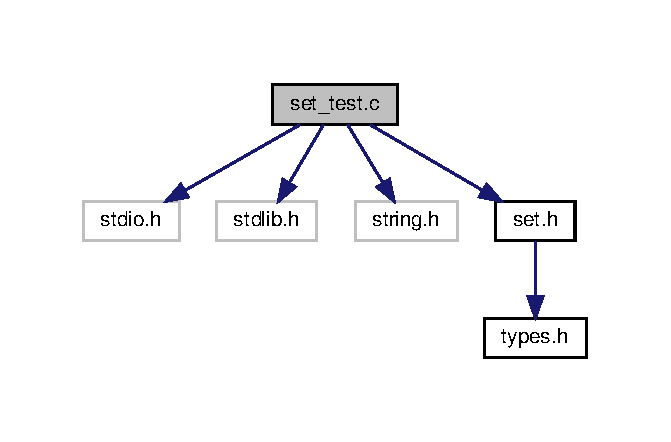
\includegraphics[width=322pt]{set__test_8c__incl}
\end{center}
\end{figure}
\subsection*{Functions}
\begin{DoxyCompactItemize}
\item 
int \hyperlink{set__test_8c_ae66f6b31b5ad750f1fe042a706a4e3d4}{main} ()
\begin{DoxyCompactList}\small\item\em funcion principal de prueba del set \end{DoxyCompactList}\end{DoxyCompactItemize}


\subsection{Detailed Description}
En este fichero probamos las funciones del set. 

\begin{DoxyAuthor}{Author}
Manuel Suarez, Saul Almazán, Álvaro Becerra, Rodrigo Lardiés 
\end{DoxyAuthor}
\begin{DoxyVersion}{Version}
1.\+0 
\end{DoxyVersion}
\begin{DoxyDate}{Date}
10/11/2018 
\end{DoxyDate}


\subsection{Function Documentation}
\mbox{\Hypertarget{set__test_8c_ae66f6b31b5ad750f1fe042a706a4e3d4}\label{set__test_8c_ae66f6b31b5ad750f1fe042a706a4e3d4}} 
\index{set\+\_\+test.\+c@{set\+\_\+test.\+c}!main@{main}}
\index{main@{main}!set\+\_\+test.\+c@{set\+\_\+test.\+c}}
\subsubsection{\texorpdfstring{main()}{main()}}
{\footnotesize\ttfamily int main (\begin{DoxyParamCaption}{ }\end{DoxyParamCaption})}



funcion principal de prueba del set 

\begin{DoxyAuthor}{Author}
Manuel Suarez, Saul Almazán, Álvaro Becerra, Rodrigo Lardiés 
\end{DoxyAuthor}
\begin{DoxyDate}{Date}
10/11/2018 
\end{DoxyDate}
\begin{DoxyReturn}{Returns}
int 
\end{DoxyReturn}

\hypertarget{space_8c}{}\section{space.\+c File Reference}
\label{space_8c}\index{space.\+c@{space.\+c}}


En este fichero implementamos las funciones de space.  


{\ttfamily \#include $<$stdio.\+h$>$}\newline
{\ttfamily \#include $<$stdlib.\+h$>$}\newline
{\ttfamily \#include $<$string.\+h$>$}\newline
{\ttfamily \#include \char`\"{}space.\+h\char`\"{}}\newline
Include dependency graph for space.\+c\+:\nopagebreak
\begin{figure}[H]
\begin{center}
\leavevmode
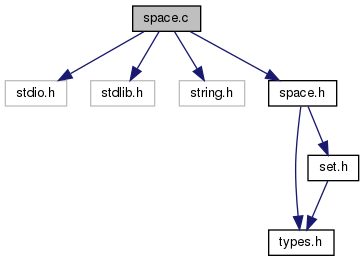
\includegraphics[width=345pt]{space_8c__incl}
\end{center}
\end{figure}
\subsection*{Classes}
\begin{DoxyCompactItemize}
\item 
struct \hyperlink{struct__Space}{\+\_\+\+Space}
\end{DoxyCompactItemize}
\subsection*{Functions}
\begin{DoxyCompactItemize}
\item 
\hyperlink{space_8h_a67533ffc2b70463baecc38fb0629bbfc}{Space} $\ast$ \hyperlink{space_8c_a162866fcea156b800fd546d0ffd271c9}{space\+\_\+create} (\hyperlink{types_8h_a845e604fb28f7e3d97549da3448149d3}{Id} id)
\begin{DoxyCompactList}\small\item\em crea un espacio \end{DoxyCompactList}\item 
\hyperlink{types_8h_a32c27cc471df37f4fc818d65de0a56c4}{S\+T\+A\+T\+US} \hyperlink{space_8c_a5c70c70398923693ddbe4dfac8d72a0d}{space\+\_\+destroy} (\hyperlink{space_8h_a67533ffc2b70463baecc38fb0629bbfc}{Space} $\ast$space)
\begin{DoxyCompactList}\small\item\em destruye y libera la memoria de un espacio \end{DoxyCompactList}\item 
\hyperlink{types_8h_a32c27cc471df37f4fc818d65de0a56c4}{S\+T\+A\+T\+US} \hyperlink{space_8c_aab5b468f9822ab78dbe16d1321870d93}{space\+\_\+set\+\_\+name} (\hyperlink{space_8h_a67533ffc2b70463baecc38fb0629bbfc}{Space} $\ast$space, char $\ast$name)
\begin{DoxyCompactList}\small\item\em cambia el nombre del espacio \end{DoxyCompactList}\item 
\hyperlink{types_8h_a32c27cc471df37f4fc818d65de0a56c4}{S\+T\+A\+T\+US} \hyperlink{space_8c_a9e6e3e3bac4996ac6b8bd555e52bfb26}{space\+\_\+set\+\_\+north} (\hyperlink{space_8h_a67533ffc2b70463baecc38fb0629bbfc}{Space} $\ast$space, \hyperlink{types_8h_a845e604fb28f7e3d97549da3448149d3}{Id} id)
\begin{DoxyCompactList}\small\item\em cambia el Id del norte del espacio \end{DoxyCompactList}\item 
\hyperlink{types_8h_a32c27cc471df37f4fc818d65de0a56c4}{S\+T\+A\+T\+US} \hyperlink{space_8c_a422ab9f220b4c471c44256a27377de1a}{space\+\_\+set\+\_\+south} (\hyperlink{space_8h_a67533ffc2b70463baecc38fb0629bbfc}{Space} $\ast$space, \hyperlink{types_8h_a845e604fb28f7e3d97549da3448149d3}{Id} id)
\begin{DoxyCompactList}\small\item\em cambia el Id del sur del espacio \end{DoxyCompactList}\item 
\hyperlink{types_8h_a32c27cc471df37f4fc818d65de0a56c4}{S\+T\+A\+T\+US} \hyperlink{space_8c_a860a8f3e0227955ad56d1a12f0bdc44a}{space\+\_\+set\+\_\+east} (\hyperlink{space_8h_a67533ffc2b70463baecc38fb0629bbfc}{Space} $\ast$space, \hyperlink{types_8h_a845e604fb28f7e3d97549da3448149d3}{Id} id)
\begin{DoxyCompactList}\small\item\em cambia el Id del este del espacio \end{DoxyCompactList}\item 
\hyperlink{types_8h_a32c27cc471df37f4fc818d65de0a56c4}{S\+T\+A\+T\+US} \hyperlink{space_8c_ad44b14cb38902cf31fa1f341beaab0db}{space\+\_\+set\+\_\+west} (\hyperlink{space_8h_a67533ffc2b70463baecc38fb0629bbfc}{Space} $\ast$space, \hyperlink{types_8h_a845e604fb28f7e3d97549da3448149d3}{Id} id)
\begin{DoxyCompactList}\small\item\em cambia el Id del oeste del espacio \end{DoxyCompactList}\item 
const char $\ast$ \hyperlink{space_8c_a310c540cd6e11073f7328add1f927001}{space\+\_\+get\+\_\+name} (\hyperlink{space_8h_a67533ffc2b70463baecc38fb0629bbfc}{Space} $\ast$space)
\begin{DoxyCompactList}\small\item\em devuelve el nombre del espacio \end{DoxyCompactList}\item 
\hyperlink{types_8h_a845e604fb28f7e3d97549da3448149d3}{Id} \hyperlink{space_8c_ac8ddfd0d8692fd852ee49698c446cb50}{space\+\_\+get\+\_\+id} (\hyperlink{space_8h_a67533ffc2b70463baecc38fb0629bbfc}{Space} $\ast$space)
\begin{DoxyCompactList}\small\item\em devuelve el Id del espacio \end{DoxyCompactList}\item 
\hyperlink{types_8h_a845e604fb28f7e3d97549da3448149d3}{Id} \hyperlink{space_8c_ad331fba774897900f615d9d2e8d81a90}{space\+\_\+get\+\_\+north} (\hyperlink{space_8h_a67533ffc2b70463baecc38fb0629bbfc}{Space} $\ast$space)
\begin{DoxyCompactList}\small\item\em devuelve el Id del norte \end{DoxyCompactList}\item 
\hyperlink{types_8h_a845e604fb28f7e3d97549da3448149d3}{Id} \hyperlink{space_8c_a9b86e1335c423eaad832e50d4c12cf1f}{space\+\_\+get\+\_\+south} (\hyperlink{space_8h_a67533ffc2b70463baecc38fb0629bbfc}{Space} $\ast$space)
\begin{DoxyCompactList}\small\item\em devuelve el Id del sur \end{DoxyCompactList}\item 
\hyperlink{types_8h_a845e604fb28f7e3d97549da3448149d3}{Id} \hyperlink{space_8c_a978a22b77f74bb2dab68a00571abbe0b}{space\+\_\+get\+\_\+east} (\hyperlink{space_8h_a67533ffc2b70463baecc38fb0629bbfc}{Space} $\ast$space)
\begin{DoxyCompactList}\small\item\em devuelve el Id del este \end{DoxyCompactList}\item 
\hyperlink{types_8h_a845e604fb28f7e3d97549da3448149d3}{Id} \hyperlink{space_8c_af495ebfd5d13eba1a48cebd10992a17f}{space\+\_\+get\+\_\+west} (\hyperlink{space_8h_a67533ffc2b70463baecc38fb0629bbfc}{Space} $\ast$space)
\begin{DoxyCompactList}\small\item\em devuelve el Id del oeste \end{DoxyCompactList}\item 
\hyperlink{types_8h_a32c27cc471df37f4fc818d65de0a56c4}{S\+T\+A\+T\+US} \hyperlink{space_8c_a18eca058da6cdf20ae5eda9d122d992e}{space\+\_\+print} (\hyperlink{space_8h_a67533ffc2b70463baecc38fb0629bbfc}{Space} $\ast$space)
\begin{DoxyCompactList}\small\item\em imprime el espacio \end{DoxyCompactList}\item 
\hyperlink{types_8h_a32c27cc471df37f4fc818d65de0a56c4}{S\+T\+A\+T\+US} \hyperlink{space_8c_af845878ae403cdd733520bb96e2385ea}{space\+\_\+take\+\_\+object} (\hyperlink{space_8h_a67533ffc2b70463baecc38fb0629bbfc}{Space} $\ast$space, \hyperlink{types_8h_a845e604fb28f7e3d97549da3448149d3}{Id} id)
\begin{DoxyCompactList}\small\item\em coge un objeto del espacio \end{DoxyCompactList}\item 
\hyperlink{types_8h_a32c27cc471df37f4fc818d65de0a56c4}{S\+T\+A\+T\+US} \hyperlink{space_8c_af038679271749a0298ba4a7c2efd46ed}{space\+\_\+leave\+\_\+object} (\hyperlink{space_8h_a67533ffc2b70463baecc38fb0629bbfc}{Space} $\ast$space, \hyperlink{types_8h_a845e604fb28f7e3d97549da3448149d3}{Id} id)
\begin{DoxyCompactList}\small\item\em suelta un objeto del espacio \end{DoxyCompactList}\item 
char $\ast$ \hyperlink{space_8c_a0dac96ce03e0ed60e3faa841f2b20b52}{space\+\_\+get\+\_\+gdesc} (\hyperlink{space_8h_a67533ffc2b70463baecc38fb0629bbfc}{Space} $\ast$space)
\begin{DoxyCompactList}\small\item\em devuelve el contenido del espacio \end{DoxyCompactList}\item 
\hyperlink{types_8h_a32c27cc471df37f4fc818d65de0a56c4}{S\+T\+A\+T\+US} \hyperlink{space_8c_a4ad8cbd4209e5a0e21318b5ffbad4669}{space\+\_\+set\+\_\+gdesc} (\hyperlink{space_8h_a67533ffc2b70463baecc38fb0629bbfc}{Space} $\ast$space, char $\ast$gdesc)
\begin{DoxyCompactList}\small\item\em cambia el contenido del espacio \end{DoxyCompactList}\item 
char $\ast$ \hyperlink{space_8c_a292ba89734c883f99015a8b6ec147be8}{space\+\_\+get\+\_\+description} (\hyperlink{space_8h_a67533ffc2b70463baecc38fb0629bbfc}{Space} $\ast$space)
\begin{DoxyCompactList}\small\item\em devuelve la descripcion del espacio \end{DoxyCompactList}\item 
\hyperlink{types_8h_a32c27cc471df37f4fc818d65de0a56c4}{S\+T\+A\+T\+US} \hyperlink{space_8c_a7aecc426029f567d452a0f916fd512d6}{space\+\_\+set\+\_\+description} (\hyperlink{space_8h_a67533ffc2b70463baecc38fb0629bbfc}{Space} $\ast$space, char $\ast$description)
\begin{DoxyCompactList}\small\item\em cambia la descripcion del espacio \end{DoxyCompactList}\item 
\hyperlink{types_8h_a3e5b8192e7d9ffaf3542f1210aec18dd}{B\+O\+OL} \hyperlink{space_8c_aac1e07503b3a4e740444c1318f6ea868}{space\+\_\+is\+\_\+object\+\_\+in} (\hyperlink{space_8h_a67533ffc2b70463baecc38fb0629bbfc}{Space} $\ast$space, \hyperlink{types_8h_a845e604fb28f7e3d97549da3448149d3}{Id} id)
\begin{DoxyCompactList}\small\item\em comprueba si hay un objeto en el espacio \end{DoxyCompactList}\end{DoxyCompactItemize}


\subsection{Detailed Description}
En este fichero implementamos las funciones de space. 

\begin{DoxyAuthor}{Author}
Manuel Suarez, Saul Almazán, Álvaro Becerra, Rodrigo Lardiés 
\end{DoxyAuthor}
\begin{DoxyVersion}{Version}
1.\+0 
\end{DoxyVersion}
\begin{DoxyDate}{Date}
20/10/2018 
\end{DoxyDate}


\subsection{Function Documentation}
\mbox{\Hypertarget{space_8c_a162866fcea156b800fd546d0ffd271c9}\label{space_8c_a162866fcea156b800fd546d0ffd271c9}} 
\index{space.\+c@{space.\+c}!space\+\_\+create@{space\+\_\+create}}
\index{space\+\_\+create@{space\+\_\+create}!space.\+c@{space.\+c}}
\subsubsection{\texorpdfstring{space\+\_\+create()}{space\_create()}}
{\footnotesize\ttfamily \hyperlink{space_8h_a67533ffc2b70463baecc38fb0629bbfc}{Space}$\ast$ space\+\_\+create (\begin{DoxyParamCaption}\item[{\hyperlink{types_8h_a845e604fb28f7e3d97549da3448149d3}{Id}}]{id }\end{DoxyParamCaption})}



crea un espacio 

\begin{DoxyAuthor}{Author}
Manuel Suarez, Saul Almazán, Álvaro Becerra, Rodrigo Lardiés 
\end{DoxyAuthor}
\begin{DoxyDate}{Date}
10/11/2018 
\end{DoxyDate}

\begin{DoxyParams}{Parameters}
{\em id} & (id del nuevo espacio) \\
\hline
\end{DoxyParams}
\begin{DoxyReturn}{Returns}
Space$\ast$ (El espacio que crea) 
\end{DoxyReturn}
\mbox{\Hypertarget{space_8c_a5c70c70398923693ddbe4dfac8d72a0d}\label{space_8c_a5c70c70398923693ddbe4dfac8d72a0d}} 
\index{space.\+c@{space.\+c}!space\+\_\+destroy@{space\+\_\+destroy}}
\index{space\+\_\+destroy@{space\+\_\+destroy}!space.\+c@{space.\+c}}
\subsubsection{\texorpdfstring{space\+\_\+destroy()}{space\_destroy()}}
{\footnotesize\ttfamily \hyperlink{types_8h_a32c27cc471df37f4fc818d65de0a56c4}{S\+T\+A\+T\+US} space\+\_\+destroy (\begin{DoxyParamCaption}\item[{\hyperlink{space_8h_a67533ffc2b70463baecc38fb0629bbfc}{Space} $\ast$}]{space }\end{DoxyParamCaption})}



destruye y libera la memoria de un espacio 

\begin{DoxyAuthor}{Author}
Manuel Suarez, Saul Almazán, Álvaro Becerra, Rodrigo Lardiés 
\end{DoxyAuthor}
\begin{DoxyDate}{Date}
10/11/2018 
\end{DoxyDate}

\begin{DoxyParams}{Parameters}
{\em space} & (el espacio a destruir) \\
\hline
\end{DoxyParams}
\begin{DoxyReturn}{Returns}
S\+T\+A\+T\+US (Ok si se ha realizado con exito o E\+R\+R\+OR de lo contrario) 
\end{DoxyReturn}
\mbox{\Hypertarget{space_8c_a292ba89734c883f99015a8b6ec147be8}\label{space_8c_a292ba89734c883f99015a8b6ec147be8}} 
\index{space.\+c@{space.\+c}!space\+\_\+get\+\_\+description@{space\+\_\+get\+\_\+description}}
\index{space\+\_\+get\+\_\+description@{space\+\_\+get\+\_\+description}!space.\+c@{space.\+c}}
\subsubsection{\texorpdfstring{space\+\_\+get\+\_\+description()}{space\_get\_description()}}
{\footnotesize\ttfamily char$\ast$ space\+\_\+get\+\_\+description (\begin{DoxyParamCaption}\item[{\hyperlink{space_8h_a67533ffc2b70463baecc38fb0629bbfc}{Space} $\ast$}]{space }\end{DoxyParamCaption})}



devuelve la descripcion del espacio 

\begin{DoxyAuthor}{Author}
Manuel Suarez, Saul Almazán, Álvaro Becerra, Rodrigo Lardiés 
\end{DoxyAuthor}
\begin{DoxyDate}{Date}
10/11/2018 
\end{DoxyDate}

\begin{DoxyParams}{Parameters}
{\em space} & (espacio a usar) \\
\hline
\end{DoxyParams}
\begin{DoxyReturn}{Returns}
char (La descripcion del espacio) 
\end{DoxyReturn}
\mbox{\Hypertarget{space_8c_a978a22b77f74bb2dab68a00571abbe0b}\label{space_8c_a978a22b77f74bb2dab68a00571abbe0b}} 
\index{space.\+c@{space.\+c}!space\+\_\+get\+\_\+east@{space\+\_\+get\+\_\+east}}
\index{space\+\_\+get\+\_\+east@{space\+\_\+get\+\_\+east}!space.\+c@{space.\+c}}
\subsubsection{\texorpdfstring{space\+\_\+get\+\_\+east()}{space\_get\_east()}}
{\footnotesize\ttfamily \hyperlink{types_8h_a845e604fb28f7e3d97549da3448149d3}{Id} space\+\_\+get\+\_\+east (\begin{DoxyParamCaption}\item[{\hyperlink{space_8h_a67533ffc2b70463baecc38fb0629bbfc}{Space} $\ast$}]{space }\end{DoxyParamCaption})}



devuelve el Id del este 

\begin{DoxyAuthor}{Author}
Manuel Suarez, Saul Almazán, Álvaro Becerra, Rodrigo Lardiés 
\end{DoxyAuthor}
\begin{DoxyDate}{Date}
10/11/2018 
\end{DoxyDate}

\begin{DoxyParams}{Parameters}
{\em space} & (espacio a usar) \\
\hline
\end{DoxyParams}
\begin{DoxyReturn}{Returns}
Id(devuelve el Id del este) 
\end{DoxyReturn}
\mbox{\Hypertarget{space_8c_a0dac96ce03e0ed60e3faa841f2b20b52}\label{space_8c_a0dac96ce03e0ed60e3faa841f2b20b52}} 
\index{space.\+c@{space.\+c}!space\+\_\+get\+\_\+gdesc@{space\+\_\+get\+\_\+gdesc}}
\index{space\+\_\+get\+\_\+gdesc@{space\+\_\+get\+\_\+gdesc}!space.\+c@{space.\+c}}
\subsubsection{\texorpdfstring{space\+\_\+get\+\_\+gdesc()}{space\_get\_gdesc()}}
{\footnotesize\ttfamily char$\ast$ space\+\_\+get\+\_\+gdesc (\begin{DoxyParamCaption}\item[{\hyperlink{space_8h_a67533ffc2b70463baecc38fb0629bbfc}{Space} $\ast$}]{space }\end{DoxyParamCaption})}



devuelve el contenido del espacio 

\begin{DoxyAuthor}{Author}
Manuel Suarez, Saul Almazán, Álvaro Becerra, Rodrigo Lardiés 
\end{DoxyAuthor}
\begin{DoxyDate}{Date}
10/11/2018 
\end{DoxyDate}

\begin{DoxyParams}{Parameters}
{\em space} & (espacio a usar) \\
\hline
\end{DoxyParams}
\begin{DoxyReturn}{Returns}
char (La informacion del espacio) 
\end{DoxyReturn}
\mbox{\Hypertarget{space_8c_ac8ddfd0d8692fd852ee49698c446cb50}\label{space_8c_ac8ddfd0d8692fd852ee49698c446cb50}} 
\index{space.\+c@{space.\+c}!space\+\_\+get\+\_\+id@{space\+\_\+get\+\_\+id}}
\index{space\+\_\+get\+\_\+id@{space\+\_\+get\+\_\+id}!space.\+c@{space.\+c}}
\subsubsection{\texorpdfstring{space\+\_\+get\+\_\+id()}{space\_get\_id()}}
{\footnotesize\ttfamily \hyperlink{types_8h_a845e604fb28f7e3d97549da3448149d3}{Id} space\+\_\+get\+\_\+id (\begin{DoxyParamCaption}\item[{\hyperlink{space_8h_a67533ffc2b70463baecc38fb0629bbfc}{Space} $\ast$}]{space }\end{DoxyParamCaption})}



devuelve el Id del espacio 

\begin{DoxyAuthor}{Author}
Manuel Suarez, Saul Almazán, Álvaro Becerra, Rodrigo Lardiés 
\end{DoxyAuthor}
\begin{DoxyDate}{Date}
10/11/2018 
\end{DoxyDate}

\begin{DoxyParams}{Parameters}
{\em space} & (espacio a usar) \\
\hline
\end{DoxyParams}
\begin{DoxyReturn}{Returns}
Id (El Id del espacio) 
\end{DoxyReturn}
\mbox{\Hypertarget{space_8c_a310c540cd6e11073f7328add1f927001}\label{space_8c_a310c540cd6e11073f7328add1f927001}} 
\index{space.\+c@{space.\+c}!space\+\_\+get\+\_\+name@{space\+\_\+get\+\_\+name}}
\index{space\+\_\+get\+\_\+name@{space\+\_\+get\+\_\+name}!space.\+c@{space.\+c}}
\subsubsection{\texorpdfstring{space\+\_\+get\+\_\+name()}{space\_get\_name()}}
{\footnotesize\ttfamily const char$\ast$ space\+\_\+get\+\_\+name (\begin{DoxyParamCaption}\item[{\hyperlink{space_8h_a67533ffc2b70463baecc38fb0629bbfc}{Space} $\ast$}]{space }\end{DoxyParamCaption})}



devuelve el nombre del espacio 

\begin{DoxyAuthor}{Author}
Manuel Suarez, Saul Almazán, Álvaro Becerra, Rodrigo Lardiés 
\end{DoxyAuthor}
\begin{DoxyDate}{Date}
10/11/2018 
\end{DoxyDate}

\begin{DoxyParams}{Parameters}
{\em space} & (espacio a usar) \\
\hline
\end{DoxyParams}
\begin{DoxyReturn}{Returns}
const char(\+El nombre del espacio) 
\end{DoxyReturn}
\mbox{\Hypertarget{space_8c_ad331fba774897900f615d9d2e8d81a90}\label{space_8c_ad331fba774897900f615d9d2e8d81a90}} 
\index{space.\+c@{space.\+c}!space\+\_\+get\+\_\+north@{space\+\_\+get\+\_\+north}}
\index{space\+\_\+get\+\_\+north@{space\+\_\+get\+\_\+north}!space.\+c@{space.\+c}}
\subsubsection{\texorpdfstring{space\+\_\+get\+\_\+north()}{space\_get\_north()}}
{\footnotesize\ttfamily \hyperlink{types_8h_a845e604fb28f7e3d97549da3448149d3}{Id} space\+\_\+get\+\_\+north (\begin{DoxyParamCaption}\item[{\hyperlink{space_8h_a67533ffc2b70463baecc38fb0629bbfc}{Space} $\ast$}]{space }\end{DoxyParamCaption})}



devuelve el Id del norte 

\begin{DoxyAuthor}{Author}
Manuel Suarez, Saul Almazán, Álvaro Becerra, Rodrigo Lardiés 
\end{DoxyAuthor}
\begin{DoxyDate}{Date}
10/11/2018 
\end{DoxyDate}

\begin{DoxyParams}{Parameters}
{\em space} & (espacio a usar) \\
\hline
\end{DoxyParams}
\begin{DoxyReturn}{Returns}
Id(devuelve el Id del norte) 
\end{DoxyReturn}
\mbox{\Hypertarget{space_8c_a9b86e1335c423eaad832e50d4c12cf1f}\label{space_8c_a9b86e1335c423eaad832e50d4c12cf1f}} 
\index{space.\+c@{space.\+c}!space\+\_\+get\+\_\+south@{space\+\_\+get\+\_\+south}}
\index{space\+\_\+get\+\_\+south@{space\+\_\+get\+\_\+south}!space.\+c@{space.\+c}}
\subsubsection{\texorpdfstring{space\+\_\+get\+\_\+south()}{space\_get\_south()}}
{\footnotesize\ttfamily \hyperlink{types_8h_a845e604fb28f7e3d97549da3448149d3}{Id} space\+\_\+get\+\_\+south (\begin{DoxyParamCaption}\item[{\hyperlink{space_8h_a67533ffc2b70463baecc38fb0629bbfc}{Space} $\ast$}]{space }\end{DoxyParamCaption})}



devuelve el Id del sur 

\begin{DoxyAuthor}{Author}
Manuel Suarez, Saul Almazán, Álvaro Becerra, Rodrigo Lardiés 
\end{DoxyAuthor}
\begin{DoxyDate}{Date}
10/11/2018 
\end{DoxyDate}

\begin{DoxyParams}{Parameters}
{\em space} & (espacio a usar) \\
\hline
\end{DoxyParams}
\begin{DoxyReturn}{Returns}
Id(devuelve el Id del sur) 
\end{DoxyReturn}
\mbox{\Hypertarget{space_8c_af495ebfd5d13eba1a48cebd10992a17f}\label{space_8c_af495ebfd5d13eba1a48cebd10992a17f}} 
\index{space.\+c@{space.\+c}!space\+\_\+get\+\_\+west@{space\+\_\+get\+\_\+west}}
\index{space\+\_\+get\+\_\+west@{space\+\_\+get\+\_\+west}!space.\+c@{space.\+c}}
\subsubsection{\texorpdfstring{space\+\_\+get\+\_\+west()}{space\_get\_west()}}
{\footnotesize\ttfamily \hyperlink{types_8h_a845e604fb28f7e3d97549da3448149d3}{Id} space\+\_\+get\+\_\+west (\begin{DoxyParamCaption}\item[{\hyperlink{space_8h_a67533ffc2b70463baecc38fb0629bbfc}{Space} $\ast$}]{space }\end{DoxyParamCaption})}



devuelve el Id del oeste 

\begin{DoxyAuthor}{Author}
Manuel Suarez, Saul Almazán, Álvaro Becerra, Rodrigo Lardiés 
\end{DoxyAuthor}
\begin{DoxyDate}{Date}
10/11/2018 
\end{DoxyDate}

\begin{DoxyParams}{Parameters}
{\em space} & (espacio a usar) \\
\hline
\end{DoxyParams}
\begin{DoxyReturn}{Returns}
Id(devuelve el Id del oeste) 
\end{DoxyReturn}
\mbox{\Hypertarget{space_8c_aac1e07503b3a4e740444c1318f6ea868}\label{space_8c_aac1e07503b3a4e740444c1318f6ea868}} 
\index{space.\+c@{space.\+c}!space\+\_\+is\+\_\+object\+\_\+in@{space\+\_\+is\+\_\+object\+\_\+in}}
\index{space\+\_\+is\+\_\+object\+\_\+in@{space\+\_\+is\+\_\+object\+\_\+in}!space.\+c@{space.\+c}}
\subsubsection{\texorpdfstring{space\+\_\+is\+\_\+object\+\_\+in()}{space\_is\_object\_in()}}
{\footnotesize\ttfamily \hyperlink{types_8h_a3e5b8192e7d9ffaf3542f1210aec18dd}{B\+O\+OL} space\+\_\+is\+\_\+object\+\_\+in (\begin{DoxyParamCaption}\item[{\hyperlink{space_8h_a67533ffc2b70463baecc38fb0629bbfc}{Space} $\ast$}]{space,  }\item[{\hyperlink{types_8h_a845e604fb28f7e3d97549da3448149d3}{Id}}]{id }\end{DoxyParamCaption})}



comprueba si hay un objeto en el espacio 

\begin{DoxyAuthor}{Author}
Manuel Suarez, Saul Almazán, Álvaro Becerra, Rodrigo Lardiés 
\end{DoxyAuthor}
\begin{DoxyDate}{Date}
10/11/2018 
\end{DoxyDate}

\begin{DoxyParams}{Parameters}
{\em space} & (espacio a usar) \\
\hline
{\em id} & (Id del objeto a comprobar) \\
\hline
\end{DoxyParams}
\begin{DoxyReturn}{Returns}
B\+O\+OL (T\+R\+UE si se el objeto esta en el espacio o F\+A\+L\+SE de lo contrario) 
\end{DoxyReturn}
\mbox{\Hypertarget{space_8c_af038679271749a0298ba4a7c2efd46ed}\label{space_8c_af038679271749a0298ba4a7c2efd46ed}} 
\index{space.\+c@{space.\+c}!space\+\_\+leave\+\_\+object@{space\+\_\+leave\+\_\+object}}
\index{space\+\_\+leave\+\_\+object@{space\+\_\+leave\+\_\+object}!space.\+c@{space.\+c}}
\subsubsection{\texorpdfstring{space\+\_\+leave\+\_\+object()}{space\_leave\_object()}}
{\footnotesize\ttfamily \hyperlink{types_8h_a32c27cc471df37f4fc818d65de0a56c4}{S\+T\+A\+T\+US} space\+\_\+leave\+\_\+object (\begin{DoxyParamCaption}\item[{\hyperlink{space_8h_a67533ffc2b70463baecc38fb0629bbfc}{Space} $\ast$}]{space,  }\item[{\hyperlink{types_8h_a845e604fb28f7e3d97549da3448149d3}{Id}}]{id }\end{DoxyParamCaption})}



suelta un objeto del espacio 

\begin{DoxyAuthor}{Author}
Manuel Suarez, Saul Almazán, Álvaro Becerra, Rodrigo Lardiés 
\end{DoxyAuthor}
\begin{DoxyDate}{Date}
10/11/2018 
\end{DoxyDate}

\begin{DoxyParams}{Parameters}
{\em space} & (espacio a usar) \\
\hline
{\em id} & (id del objeto a soltar) \\
\hline
\end{DoxyParams}
\begin{DoxyReturn}{Returns}
S\+T\+A\+T\+US (OK si se suelta bien o E\+R\+R\+OR de lo contrario) 
\end{DoxyReturn}
\mbox{\Hypertarget{space_8c_a18eca058da6cdf20ae5eda9d122d992e}\label{space_8c_a18eca058da6cdf20ae5eda9d122d992e}} 
\index{space.\+c@{space.\+c}!space\+\_\+print@{space\+\_\+print}}
\index{space\+\_\+print@{space\+\_\+print}!space.\+c@{space.\+c}}
\subsubsection{\texorpdfstring{space\+\_\+print()}{space\_print()}}
{\footnotesize\ttfamily \hyperlink{types_8h_a32c27cc471df37f4fc818d65de0a56c4}{S\+T\+A\+T\+US} space\+\_\+print (\begin{DoxyParamCaption}\item[{\hyperlink{space_8h_a67533ffc2b70463baecc38fb0629bbfc}{Space} $\ast$}]{space }\end{DoxyParamCaption})}



imprime el espacio 

\begin{DoxyAuthor}{Author}
Manuel Suarez, Saul Almazán, Álvaro Becerra, Rodrigo Lardiés 
\end{DoxyAuthor}
\begin{DoxyDate}{Date}
10/11/2018 
\end{DoxyDate}

\begin{DoxyParams}{Parameters}
{\em space} & (espacio a usar) \\
\hline
\end{DoxyParams}
\begin{DoxyReturn}{Returns}
S\+T\+A\+T\+US (Ok si se imprime bien o E\+R\+R\+OR de lo contrario) 
\end{DoxyReturn}
\mbox{\Hypertarget{space_8c_a7aecc426029f567d452a0f916fd512d6}\label{space_8c_a7aecc426029f567d452a0f916fd512d6}} 
\index{space.\+c@{space.\+c}!space\+\_\+set\+\_\+description@{space\+\_\+set\+\_\+description}}
\index{space\+\_\+set\+\_\+description@{space\+\_\+set\+\_\+description}!space.\+c@{space.\+c}}
\subsubsection{\texorpdfstring{space\+\_\+set\+\_\+description()}{space\_set\_description()}}
{\footnotesize\ttfamily \hyperlink{types_8h_a32c27cc471df37f4fc818d65de0a56c4}{S\+T\+A\+T\+US} space\+\_\+set\+\_\+description (\begin{DoxyParamCaption}\item[{\hyperlink{space_8h_a67533ffc2b70463baecc38fb0629bbfc}{Space} $\ast$}]{space,  }\item[{char $\ast$}]{description }\end{DoxyParamCaption})}



cambia la descripcion del espacio 

\begin{DoxyAuthor}{Author}
Manuel Suarez, Saul Almazán, Álvaro Becerra, Rodrigo Lardiés 
\end{DoxyAuthor}
\begin{DoxyDate}{Date}
10/11/2018 
\end{DoxyDate}

\begin{DoxyParams}{Parameters}
{\em space} & (espacio a usar) \\
\hline
{\em description} & (La descripcion del espacio) \\
\hline
\end{DoxyParams}
\begin{DoxyReturn}{Returns}
S\+T\+A\+T\+US (OK si se modifica bien o E\+R\+R\+OR de lo contrario) 
\end{DoxyReturn}
\mbox{\Hypertarget{space_8c_a860a8f3e0227955ad56d1a12f0bdc44a}\label{space_8c_a860a8f3e0227955ad56d1a12f0bdc44a}} 
\index{space.\+c@{space.\+c}!space\+\_\+set\+\_\+east@{space\+\_\+set\+\_\+east}}
\index{space\+\_\+set\+\_\+east@{space\+\_\+set\+\_\+east}!space.\+c@{space.\+c}}
\subsubsection{\texorpdfstring{space\+\_\+set\+\_\+east()}{space\_set\_east()}}
{\footnotesize\ttfamily \hyperlink{types_8h_a32c27cc471df37f4fc818d65de0a56c4}{S\+T\+A\+T\+US} space\+\_\+set\+\_\+east (\begin{DoxyParamCaption}\item[{\hyperlink{space_8h_a67533ffc2b70463baecc38fb0629bbfc}{Space} $\ast$}]{space,  }\item[{\hyperlink{types_8h_a845e604fb28f7e3d97549da3448149d3}{Id}}]{id }\end{DoxyParamCaption})}



cambia el Id del este del espacio 

\begin{DoxyAuthor}{Author}
Manuel Suarez, Saul Almazán, Álvaro Becerra, Rodrigo Lardiés 
\end{DoxyAuthor}
\begin{DoxyDate}{Date}
10/11/2018 
\end{DoxyDate}

\begin{DoxyParams}{Parameters}
{\em space} & (espacio a usar) \\
\hline
{\em id} & (Id nuevo para el este) \\
\hline
\end{DoxyParams}
\begin{DoxyReturn}{Returns}
S\+T\+A\+T\+US (OK si se ha realizado con exito o E\+R\+R\+OR de lo contrario) 
\end{DoxyReturn}
\mbox{\Hypertarget{space_8c_a4ad8cbd4209e5a0e21318b5ffbad4669}\label{space_8c_a4ad8cbd4209e5a0e21318b5ffbad4669}} 
\index{space.\+c@{space.\+c}!space\+\_\+set\+\_\+gdesc@{space\+\_\+set\+\_\+gdesc}}
\index{space\+\_\+set\+\_\+gdesc@{space\+\_\+set\+\_\+gdesc}!space.\+c@{space.\+c}}
\subsubsection{\texorpdfstring{space\+\_\+set\+\_\+gdesc()}{space\_set\_gdesc()}}
{\footnotesize\ttfamily \hyperlink{types_8h_a32c27cc471df37f4fc818d65de0a56c4}{S\+T\+A\+T\+US} space\+\_\+set\+\_\+gdesc (\begin{DoxyParamCaption}\item[{\hyperlink{space_8h_a67533ffc2b70463baecc38fb0629bbfc}{Space} $\ast$}]{space,  }\item[{char $\ast$}]{gdesc }\end{DoxyParamCaption})}



cambia el contenido del espacio 

\begin{DoxyAuthor}{Author}
Manuel Suarez, Saul Almazán, Álvaro Becerra, Rodrigo Lardiés 
\end{DoxyAuthor}
\begin{DoxyDate}{Date}
10/11/2018 
\end{DoxyDate}

\begin{DoxyParams}{Parameters}
{\em space} & (espacio a usar) \\
\hline
{\em gdesc} & (La informacion del espacio) \\
\hline
\end{DoxyParams}
\begin{DoxyReturn}{Returns}
S\+T\+A\+T\+US (OK si se modifica bien o E\+R\+R\+OR de lo contrario) 
\end{DoxyReturn}
\mbox{\Hypertarget{space_8c_aab5b468f9822ab78dbe16d1321870d93}\label{space_8c_aab5b468f9822ab78dbe16d1321870d93}} 
\index{space.\+c@{space.\+c}!space\+\_\+set\+\_\+name@{space\+\_\+set\+\_\+name}}
\index{space\+\_\+set\+\_\+name@{space\+\_\+set\+\_\+name}!space.\+c@{space.\+c}}
\subsubsection{\texorpdfstring{space\+\_\+set\+\_\+name()}{space\_set\_name()}}
{\footnotesize\ttfamily \hyperlink{types_8h_a32c27cc471df37f4fc818d65de0a56c4}{S\+T\+A\+T\+US} space\+\_\+set\+\_\+name (\begin{DoxyParamCaption}\item[{\hyperlink{space_8h_a67533ffc2b70463baecc38fb0629bbfc}{Space} $\ast$}]{space,  }\item[{char $\ast$}]{name }\end{DoxyParamCaption})}



cambia el nombre del espacio 

\begin{DoxyAuthor}{Author}
Manuel Suarez, Saul Almazán, Álvaro Becerra, Rodrigo Lardiés 
\end{DoxyAuthor}
\begin{DoxyDate}{Date}
10/11/2018 
\end{DoxyDate}

\begin{DoxyParams}{Parameters}
{\em space} & (espacio a usar) \\
\hline
{\em name} & (nuevo nombre) \\
\hline
\end{DoxyParams}
\begin{DoxyReturn}{Returns}
S\+T\+A\+T\+US (OK si se realiza con exito o E\+R\+R\+OR de lo contrario) 
\end{DoxyReturn}
\mbox{\Hypertarget{space_8c_a9e6e3e3bac4996ac6b8bd555e52bfb26}\label{space_8c_a9e6e3e3bac4996ac6b8bd555e52bfb26}} 
\index{space.\+c@{space.\+c}!space\+\_\+set\+\_\+north@{space\+\_\+set\+\_\+north}}
\index{space\+\_\+set\+\_\+north@{space\+\_\+set\+\_\+north}!space.\+c@{space.\+c}}
\subsubsection{\texorpdfstring{space\+\_\+set\+\_\+north()}{space\_set\_north()}}
{\footnotesize\ttfamily \hyperlink{types_8h_a32c27cc471df37f4fc818d65de0a56c4}{S\+T\+A\+T\+US} space\+\_\+set\+\_\+north (\begin{DoxyParamCaption}\item[{\hyperlink{space_8h_a67533ffc2b70463baecc38fb0629bbfc}{Space} $\ast$}]{space,  }\item[{\hyperlink{types_8h_a845e604fb28f7e3d97549da3448149d3}{Id}}]{id }\end{DoxyParamCaption})}



cambia el Id del norte del espacio 

\begin{DoxyAuthor}{Author}
Manuel Suarez, Saul Almazán, Álvaro Becerra, Rodrigo Lardiés 
\end{DoxyAuthor}
\begin{DoxyDate}{Date}
10/11/2018 
\end{DoxyDate}

\begin{DoxyParams}{Parameters}
{\em space} & (espacio a usar) \\
\hline
{\em id} & (Id nuevo para el norte) \\
\hline
\end{DoxyParams}
\begin{DoxyReturn}{Returns}
S\+T\+A\+T\+US (OK si se ha realizado con exito o E\+R\+R\+OR de lo contrario) 
\end{DoxyReturn}
\mbox{\Hypertarget{space_8c_a422ab9f220b4c471c44256a27377de1a}\label{space_8c_a422ab9f220b4c471c44256a27377de1a}} 
\index{space.\+c@{space.\+c}!space\+\_\+set\+\_\+south@{space\+\_\+set\+\_\+south}}
\index{space\+\_\+set\+\_\+south@{space\+\_\+set\+\_\+south}!space.\+c@{space.\+c}}
\subsubsection{\texorpdfstring{space\+\_\+set\+\_\+south()}{space\_set\_south()}}
{\footnotesize\ttfamily \hyperlink{types_8h_a32c27cc471df37f4fc818d65de0a56c4}{S\+T\+A\+T\+US} space\+\_\+set\+\_\+south (\begin{DoxyParamCaption}\item[{\hyperlink{space_8h_a67533ffc2b70463baecc38fb0629bbfc}{Space} $\ast$}]{space,  }\item[{\hyperlink{types_8h_a845e604fb28f7e3d97549da3448149d3}{Id}}]{id }\end{DoxyParamCaption})}



cambia el Id del sur del espacio 

\begin{DoxyAuthor}{Author}
Manuel Suarez, Saul Almazán, Álvaro Becerra, Rodrigo Lardiés 
\end{DoxyAuthor}
\begin{DoxyDate}{Date}
10/11/2018 
\end{DoxyDate}

\begin{DoxyParams}{Parameters}
{\em space} & (espacio a usar) \\
\hline
{\em id} & (Id nuevo para el sur) \\
\hline
\end{DoxyParams}
\begin{DoxyReturn}{Returns}
S\+T\+A\+T\+US (OK si se ha realizado con exito o E\+R\+R\+OR de lo contrario) 
\end{DoxyReturn}
\mbox{\Hypertarget{space_8c_ad44b14cb38902cf31fa1f341beaab0db}\label{space_8c_ad44b14cb38902cf31fa1f341beaab0db}} 
\index{space.\+c@{space.\+c}!space\+\_\+set\+\_\+west@{space\+\_\+set\+\_\+west}}
\index{space\+\_\+set\+\_\+west@{space\+\_\+set\+\_\+west}!space.\+c@{space.\+c}}
\subsubsection{\texorpdfstring{space\+\_\+set\+\_\+west()}{space\_set\_west()}}
{\footnotesize\ttfamily \hyperlink{types_8h_a32c27cc471df37f4fc818d65de0a56c4}{S\+T\+A\+T\+US} space\+\_\+set\+\_\+west (\begin{DoxyParamCaption}\item[{\hyperlink{space_8h_a67533ffc2b70463baecc38fb0629bbfc}{Space} $\ast$}]{space,  }\item[{\hyperlink{types_8h_a845e604fb28f7e3d97549da3448149d3}{Id}}]{id }\end{DoxyParamCaption})}



cambia el Id del oeste del espacio 

\begin{DoxyAuthor}{Author}
Manuel Suarez, Saul Almazán, Álvaro Becerra, Rodrigo Lardiés 
\end{DoxyAuthor}
\begin{DoxyDate}{Date}
10/11/2018 
\end{DoxyDate}

\begin{DoxyParams}{Parameters}
{\em space} & (espacio a usar) \\
\hline
{\em id} & (Id nuevo para el oeste) \\
\hline
\end{DoxyParams}
\begin{DoxyReturn}{Returns}
S\+T\+A\+T\+US (OK si se ha realizado con exito o E\+R\+R\+OR de lo contrario) 
\end{DoxyReturn}
\mbox{\Hypertarget{space_8c_af845878ae403cdd733520bb96e2385ea}\label{space_8c_af845878ae403cdd733520bb96e2385ea}} 
\index{space.\+c@{space.\+c}!space\+\_\+take\+\_\+object@{space\+\_\+take\+\_\+object}}
\index{space\+\_\+take\+\_\+object@{space\+\_\+take\+\_\+object}!space.\+c@{space.\+c}}
\subsubsection{\texorpdfstring{space\+\_\+take\+\_\+object()}{space\_take\_object()}}
{\footnotesize\ttfamily \hyperlink{types_8h_a32c27cc471df37f4fc818d65de0a56c4}{S\+T\+A\+T\+US} space\+\_\+take\+\_\+object (\begin{DoxyParamCaption}\item[{\hyperlink{space_8h_a67533ffc2b70463baecc38fb0629bbfc}{Space} $\ast$}]{space,  }\item[{\hyperlink{types_8h_a845e604fb28f7e3d97549da3448149d3}{Id}}]{id }\end{DoxyParamCaption})}



coge un objeto del espacio 

\begin{DoxyAuthor}{Author}
Manuel Suarez, Saul Almazán, Álvaro Becerra, Rodrigo Lardiés 
\end{DoxyAuthor}
\begin{DoxyDate}{Date}
10/11/2018 
\end{DoxyDate}

\begin{DoxyParams}{Parameters}
{\em space} & (espacio a usar) \\
\hline
{\em id} & (id del objeto a coger) \\
\hline
\end{DoxyParams}
\begin{DoxyReturn}{Returns}
S\+T\+A\+T\+US (OK si se coge bien o E\+R\+R\+OR de lo contrario) 
\end{DoxyReturn}

\hypertarget{space__test_8c}{}\section{src/space\+\_\+test.c File Reference}
\label{space__test_8c}\index{src/space\+\_\+test.\+c@{src/space\+\_\+test.\+c}}


Prueba del modulo space.  


{\ttfamily \#include $<$stdio.\+h$>$}\newline
{\ttfamily \#include $<$stdlib.\+h$>$}\newline
{\ttfamily \#include $<$string.\+h$>$}\newline
{\ttfamily \#include \char`\"{}space.\+h\char`\"{}}\newline
{\ttfamily \#include \char`\"{}space\+\_\+test.\+h\char`\"{}}\newline
{\ttfamily \#include \char`\"{}test.\+h\char`\"{}}\newline
Include dependency graph for space\+\_\+test.\+c\+:
% FIG 0
\subsection*{Macros}
\begin{DoxyCompactItemize}
\item 
\#define \hyperlink{space__test_8c_a2a77d2f2c5b698c69c19e1f8782bf709}{M\+A\+X\+\_\+\+T\+E\+S\+TS}~37
\end{DoxyCompactItemize}
\subsection*{Functions}
\begin{DoxyCompactItemize}
\item 
int \hyperlink{space__test_8c_a3c04138a5bfe5d72780bb7e82a18e627}{main} (int argc, char $\ast$$\ast$argv)
\begin{DoxyCompactList}\small\item\em Funcion principal de pruebas para el modulo Space. \end{DoxyCompactList}\item 
void \hyperlink{space__test_8c_a69278cc022dc5688d4725f8d36317b30}{test1\+\_\+space\+\_\+create} ()
\item 
void \hyperlink{space__test_8c_a2569bab6cfeec15f722d232bb8c78c9e}{test1\+\_\+space\+\_\+set\+\_\+name} ()
\item 
void \hyperlink{space__test_8c_a5a868ba017602ba6b58447cb394e81a6}{test2\+\_\+space\+\_\+set\+\_\+name} ()
\item 
void \hyperlink{space__test_8c_aa24a337830006e33706ab6ac1c416b47}{test3\+\_\+space\+\_\+set\+\_\+name} ()
\item 
void \hyperlink{space__test_8c_a3d3457a89f705948102cf1e5d4a7b45b}{test1\+\_\+space\+\_\+set\+\_\+north} ()
\item 
void \hyperlink{space__test_8c_a3bc7fe26c1e36ffd195099a9983206e1}{test2\+\_\+space\+\_\+set\+\_\+north} ()
\item 
void \hyperlink{space__test_8c_a21938e16547b3080e9251f960117a859}{test1\+\_\+space\+\_\+set\+\_\+south} ()
\item 
void \hyperlink{space__test_8c_ac9f950741f12ccfcc5ad5d9e71d3d90a}{test2\+\_\+space\+\_\+set\+\_\+south} ()
\item 
void \hyperlink{space__test_8c_ab1f093af4be3ca8e525d0517cc846f47}{test1\+\_\+space\+\_\+set\+\_\+east} ()
\item 
void \hyperlink{space__test_8c_a5df66d103388be4518c379b224f53770}{test2\+\_\+space\+\_\+set\+\_\+east} ()
\item 
void \hyperlink{space__test_8c_ab680a8797f793dffd58546074b87d21f}{test1\+\_\+space\+\_\+set\+\_\+west} ()
\item 
void \hyperlink{space__test_8c_aa51b05ffd99b7bbd8f2dfc23c8f85870}{test2\+\_\+space\+\_\+set\+\_\+west} ()
\item 
void \hyperlink{space__test_8c_ad12c42523c517507566c5c68b1527689}{test1\+\_\+space\+\_\+get\+\_\+name} ()
\item 
void \hyperlink{space__test_8c_aee88ed31c63efc674051a4563aed86e2}{test2\+\_\+space\+\_\+get\+\_\+name} ()
\item 
void \hyperlink{space__test_8c_af97836868998ad4048dcce7bc92ba773}{test1\+\_\+space\+\_\+take\+\_\+object} ()
\item 
void \hyperlink{space__test_8c_a7bc20aaf065fab5ce11288a0f1d3dfab}{test2\+\_\+space\+\_\+take\+\_\+object} ()
\item 
void \hyperlink{space__test_8c_adf86020407e0f061eac304e879029cb8}{test3\+\_\+space\+\_\+take\+\_\+object} ()
\item 
void \hyperlink{space__test_8c_a3a87f1e1e173d622bfbd3bcd14e060ca}{test1\+\_\+space\+\_\+get\+\_\+north} ()
\item 
void \hyperlink{space__test_8c_a61891c9cebb9d26dc9f149ad8341517c}{test2\+\_\+space\+\_\+get\+\_\+north} ()
\item 
void \hyperlink{space__test_8c_a8e345065f58565e131bdb3a9d0096ed5}{test1\+\_\+space\+\_\+get\+\_\+south} ()
\item 
void \hyperlink{space__test_8c_a40fe07c07c1069023b362a9e506c4c59}{test2\+\_\+space\+\_\+get\+\_\+south} ()
\item 
void \hyperlink{space__test_8c_a354adb2722b06ec65b7212d2736d6417}{test1\+\_\+space\+\_\+get\+\_\+east} ()
\item 
void \hyperlink{space__test_8c_a249293510e61c6d5465f52c14343d02b}{test2\+\_\+space\+\_\+get\+\_\+east} ()
\item 
void \hyperlink{space__test_8c_a1f08c6866885bfc093717f57b1b86539}{test1\+\_\+space\+\_\+get\+\_\+west} ()
\item 
void \hyperlink{space__test_8c_af1cf02b01c007aec0684186b39666c32}{test2\+\_\+space\+\_\+get\+\_\+west} ()
\item 
void \hyperlink{space__test_8c_a920df9e02482f4f1e6a5ebcaec523860}{test1\+\_\+space\+\_\+get\+\_\+id} ()
\item 
void \hyperlink{space__test_8c_af9087176b0d3c41d83a17a4918b13e31}{test2\+\_\+space\+\_\+get\+\_\+id} ()
\item 
void \hyperlink{space__test_8c_aeaacecb0999daa6ec764aa79ceb2a1b6}{test1\+\_\+space\+\_\+leave\+\_\+object} ()
\item 
void \hyperlink{space__test_8c_a5f23a9a66b003080f810ab44bed35560}{test2\+\_\+space\+\_\+leave\+\_\+object} ()
\item 
void \hyperlink{space__test_8c_a068c22b91236896ae1b077a8f7059458}{test1\+\_\+space\+\_\+set\+\_\+gdesc} ()
\item 
void \hyperlink{space__test_8c_af40c7a664b529a39c3d98dca3d0af708}{test2\+\_\+space\+\_\+set\+\_\+gdesc} ()
\item 
void \hyperlink{space__test_8c_a3b6d16613ee2f3940fe7c92f3934508a}{test1\+\_\+space\+\_\+get\+\_\+gdesc} ()
\item 
void \hyperlink{space__test_8c_a3422f19fd8a821a06ccba2feb52034c2}{test2\+\_\+space\+\_\+get\+\_\+gdesc} ()
\item 
void \hyperlink{space__test_8c_a19a1bac3ab9cc6f5bf7ea8c4a72392c4}{test1\+\_\+space\+\_\+set\+\_\+description} ()
\item 
void \hyperlink{space__test_8c_ab3dd07cbead60f87866e2bd2c426da0f}{test2\+\_\+space\+\_\+set\+\_\+description} ()
\item 
void \hyperlink{space__test_8c_a9a9da97ed6f49f2ae325177caecfea9c}{test1\+\_\+space\+\_\+get\+\_\+description} ()
\item 
void \hyperlink{space__test_8c_aebfa57e927e8f871e73425975c11976b}{test2\+\_\+space\+\_\+get\+\_\+description} ()
\end{DoxyCompactItemize}


\subsection{Detailed Description}
Prueba del modulo space. 

\begin{DoxyAuthor}{Author}
Manuel Suarez, Saul Almazán, �?lvaro Becerra, Rodrigo Lardiés 
\end{DoxyAuthor}
\begin{DoxyVersion}{Version}
1.\+0 
\end{DoxyVersion}
\begin{DoxyDate}{Date}
12-\/11-\/2018 
\end{DoxyDate}


\subsection{Macro Definition Documentation}
\mbox{\Hypertarget{space__test_8c_a2a77d2f2c5b698c69c19e1f8782bf709}\label{space__test_8c_a2a77d2f2c5b698c69c19e1f8782bf709}} 
\index{space\+\_\+test.\+c@{space\+\_\+test.\+c}!M\+A\+X\+\_\+\+T\+E\+S\+TS@{M\+A\+X\+\_\+\+T\+E\+S\+TS}}
\index{M\+A\+X\+\_\+\+T\+E\+S\+TS@{M\+A\+X\+\_\+\+T\+E\+S\+TS}!space\+\_\+test.\+c@{space\+\_\+test.\+c}}
\subsubsection{\texorpdfstring{M\+A\+X\+\_\+\+T\+E\+S\+TS}{MAX\_TESTS}}
{\footnotesize\ttfamily \#define M\+A\+X\+\_\+\+T\+E\+S\+TS~37}

T\+A\+M\+\_\+\+T\+E\+S\+TS 

\subsection{Function Documentation}
\mbox{\Hypertarget{space__test_8c_a3c04138a5bfe5d72780bb7e82a18e627}\label{space__test_8c_a3c04138a5bfe5d72780bb7e82a18e627}} 
\index{space\+\_\+test.\+c@{space\+\_\+test.\+c}!main@{main}}
\index{main@{main}!space\+\_\+test.\+c@{space\+\_\+test.\+c}}
\subsubsection{\texorpdfstring{main()}{main()}}
{\footnotesize\ttfamily int main (\begin{DoxyParamCaption}\item[{int}]{argc,  }\item[{char $\ast$$\ast$}]{argv }\end{DoxyParamCaption})}



Funcion principal de pruebas para el modulo Space. 

Dos modos de ejecucion\+: 1.-\/\+Si se ejecuta sin parametros se ejecutan todas las pruebas 2.-\/\+Si se ejecuta con un numero entre 1 y el numero de pruebas solo ejecuta la prueba indicada \mbox{\Hypertarget{space__test_8c_a69278cc022dc5688d4725f8d36317b30}\label{space__test_8c_a69278cc022dc5688d4725f8d36317b30}} 
\index{space\+\_\+test.\+c@{space\+\_\+test.\+c}!test1\+\_\+space\+\_\+create@{test1\+\_\+space\+\_\+create}}
\index{test1\+\_\+space\+\_\+create@{test1\+\_\+space\+\_\+create}!space\+\_\+test.\+c@{space\+\_\+test.\+c}}
\subsubsection{\texorpdfstring{test1\+\_\+space\+\_\+create()}{test1\_space\_create()}}
{\footnotesize\ttfamily void test1\+\_\+space\+\_\+create (\begin{DoxyParamCaption}{ }\end{DoxyParamCaption})}

\begin{DoxyRefDesc}{Test}
\item[\hyperlink{test__test000121}{Test}]Prueba la función de creación de un espacio \end{DoxyRefDesc}
\begin{DoxyPrecond}{Precondition}
Nada 
\end{DoxyPrecond}
\begin{DoxyPostcond}{Postcondition}
Un puntero no nulo al espacio creado 
\end{DoxyPostcond}
\mbox{\Hypertarget{space__test_8c_a9a9da97ed6f49f2ae325177caecfea9c}\label{space__test_8c_a9a9da97ed6f49f2ae325177caecfea9c}} 
\index{space\+\_\+test.\+c@{space\+\_\+test.\+c}!test1\+\_\+space\+\_\+get\+\_\+description@{test1\+\_\+space\+\_\+get\+\_\+description}}
\index{test1\+\_\+space\+\_\+get\+\_\+description@{test1\+\_\+space\+\_\+get\+\_\+description}!space\+\_\+test.\+c@{space\+\_\+test.\+c}}
\subsubsection{\texorpdfstring{test1\+\_\+space\+\_\+get\+\_\+description()}{test1\_space\_get\_description()}}
{\footnotesize\ttfamily void test1\+\_\+space\+\_\+get\+\_\+description (\begin{DoxyParamCaption}{ }\end{DoxyParamCaption})}

\begin{DoxyRefDesc}{Test}
\item[\hyperlink{test__test000156}{Test}]Prueba la función para obtener una descripcion en un espacio \end{DoxyRefDesc}
\begin{DoxyPrecond}{Precondition}
Espacio con una descripcion 
\end{DoxyPrecond}
\begin{DoxyPostcond}{Postcondition}
La salida debe ser una comparación de cadenas igual a 0 
\end{DoxyPostcond}
\mbox{\Hypertarget{space__test_8c_a354adb2722b06ec65b7212d2736d6417}\label{space__test_8c_a354adb2722b06ec65b7212d2736d6417}} 
\index{space\+\_\+test.\+c@{space\+\_\+test.\+c}!test1\+\_\+space\+\_\+get\+\_\+east@{test1\+\_\+space\+\_\+get\+\_\+east}}
\index{test1\+\_\+space\+\_\+get\+\_\+east@{test1\+\_\+space\+\_\+get\+\_\+east}!space\+\_\+test.\+c@{space\+\_\+test.\+c}}
\subsubsection{\texorpdfstring{test1\+\_\+space\+\_\+get\+\_\+east()}{test1\_space\_get\_east()}}
{\footnotesize\ttfamily void test1\+\_\+space\+\_\+get\+\_\+east (\begin{DoxyParamCaption}{ }\end{DoxyParamCaption})}

\begin{DoxyRefDesc}{Test}
\item[\hyperlink{test__test000142}{Test}]Prueba la función para obtener el este de un espacio \end{DoxyRefDesc}
\begin{DoxyPrecond}{Precondition}
Espacio con este asignado 
\end{DoxyPrecond}
\begin{DoxyPostcond}{Postcondition}
La salida debe ser id=4 
\end{DoxyPostcond}
\mbox{\Hypertarget{space__test_8c_a3b6d16613ee2f3940fe7c92f3934508a}\label{space__test_8c_a3b6d16613ee2f3940fe7c92f3934508a}} 
\index{space\+\_\+test.\+c@{space\+\_\+test.\+c}!test1\+\_\+space\+\_\+get\+\_\+gdesc@{test1\+\_\+space\+\_\+get\+\_\+gdesc}}
\index{test1\+\_\+space\+\_\+get\+\_\+gdesc@{test1\+\_\+space\+\_\+get\+\_\+gdesc}!space\+\_\+test.\+c@{space\+\_\+test.\+c}}
\subsubsection{\texorpdfstring{test1\+\_\+space\+\_\+get\+\_\+gdesc()}{test1\_space\_get\_gdesc()}}
{\footnotesize\ttfamily void test1\+\_\+space\+\_\+get\+\_\+gdesc (\begin{DoxyParamCaption}{ }\end{DoxyParamCaption})}

\begin{DoxyRefDesc}{Test}
\item[\hyperlink{test__test000152}{Test}]Prueba la función para dejar un obtener un dibujo en un espacio \end{DoxyRefDesc}
\begin{DoxyPrecond}{Precondition}
Espacio con dibujo 
\end{DoxyPrecond}
\begin{DoxyPostcond}{Postcondition}
La salida debe ser una comparacion de cadenas igual a 0 
\end{DoxyPostcond}
\mbox{\Hypertarget{space__test_8c_a920df9e02482f4f1e6a5ebcaec523860}\label{space__test_8c_a920df9e02482f4f1e6a5ebcaec523860}} 
\index{space\+\_\+test.\+c@{space\+\_\+test.\+c}!test1\+\_\+space\+\_\+get\+\_\+id@{test1\+\_\+space\+\_\+get\+\_\+id}}
\index{test1\+\_\+space\+\_\+get\+\_\+id@{test1\+\_\+space\+\_\+get\+\_\+id}!space\+\_\+test.\+c@{space\+\_\+test.\+c}}
\subsubsection{\texorpdfstring{test1\+\_\+space\+\_\+get\+\_\+id()}{test1\_space\_get\_id()}}
{\footnotesize\ttfamily void test1\+\_\+space\+\_\+get\+\_\+id (\begin{DoxyParamCaption}{ }\end{DoxyParamCaption})}

\begin{DoxyRefDesc}{Test}
\item[\hyperlink{test__test000146}{Test}]Prueba la función para obtener el id de un espacio \end{DoxyRefDesc}
\begin{DoxyPrecond}{Precondition}
Espacio con id asignado 
\end{DoxyPrecond}
\begin{DoxyPostcond}{Postcondition}
La salida debe ser id=5 
\end{DoxyPostcond}
\mbox{\Hypertarget{space__test_8c_ad12c42523c517507566c5c68b1527689}\label{space__test_8c_ad12c42523c517507566c5c68b1527689}} 
\index{space\+\_\+test.\+c@{space\+\_\+test.\+c}!test1\+\_\+space\+\_\+get\+\_\+name@{test1\+\_\+space\+\_\+get\+\_\+name}}
\index{test1\+\_\+space\+\_\+get\+\_\+name@{test1\+\_\+space\+\_\+get\+\_\+name}!space\+\_\+test.\+c@{space\+\_\+test.\+c}}
\subsubsection{\texorpdfstring{test1\+\_\+space\+\_\+get\+\_\+name()}{test1\_space\_get\_name()}}
{\footnotesize\ttfamily void test1\+\_\+space\+\_\+get\+\_\+name (\begin{DoxyParamCaption}{ }\end{DoxyParamCaption})}

\begin{DoxyRefDesc}{Test}
\item[\hyperlink{test__test000133}{Test}]Prueba la función para obtener el nombre de un espacio \end{DoxyRefDesc}
\begin{DoxyPrecond}{Precondition}
Espacio con nombre establecido 
\end{DoxyPrecond}
\begin{DoxyPostcond}{Postcondition}
La salida debe ser una comparación de cadenas igual a 0 
\end{DoxyPostcond}
\mbox{\Hypertarget{space__test_8c_a3a87f1e1e173d622bfbd3bcd14e060ca}\label{space__test_8c_a3a87f1e1e173d622bfbd3bcd14e060ca}} 
\index{space\+\_\+test.\+c@{space\+\_\+test.\+c}!test1\+\_\+space\+\_\+get\+\_\+north@{test1\+\_\+space\+\_\+get\+\_\+north}}
\index{test1\+\_\+space\+\_\+get\+\_\+north@{test1\+\_\+space\+\_\+get\+\_\+north}!space\+\_\+test.\+c@{space\+\_\+test.\+c}}
\subsubsection{\texorpdfstring{test1\+\_\+space\+\_\+get\+\_\+north()}{test1\_space\_get\_north()}}
{\footnotesize\ttfamily void test1\+\_\+space\+\_\+get\+\_\+north (\begin{DoxyParamCaption}{ }\end{DoxyParamCaption})}

\begin{DoxyRefDesc}{Test}
\item[\hyperlink{test__test000138}{Test}]Prueba la función para obtener el norte de un espacio \end{DoxyRefDesc}
\begin{DoxyPrecond}{Precondition}
Espacio con norte asignado 
\end{DoxyPrecond}
\begin{DoxyPostcond}{Postcondition}
La salida debe ser id=4 
\end{DoxyPostcond}
\mbox{\Hypertarget{space__test_8c_a8e345065f58565e131bdb3a9d0096ed5}\label{space__test_8c_a8e345065f58565e131bdb3a9d0096ed5}} 
\index{space\+\_\+test.\+c@{space\+\_\+test.\+c}!test1\+\_\+space\+\_\+get\+\_\+south@{test1\+\_\+space\+\_\+get\+\_\+south}}
\index{test1\+\_\+space\+\_\+get\+\_\+south@{test1\+\_\+space\+\_\+get\+\_\+south}!space\+\_\+test.\+c@{space\+\_\+test.\+c}}
\subsubsection{\texorpdfstring{test1\+\_\+space\+\_\+get\+\_\+south()}{test1\_space\_get\_south()}}
{\footnotesize\ttfamily void test1\+\_\+space\+\_\+get\+\_\+south (\begin{DoxyParamCaption}{ }\end{DoxyParamCaption})}

\begin{DoxyRefDesc}{Test}
\item[\hyperlink{test__test000140}{Test}]Prueba la función para obtener el sur de un espacio \end{DoxyRefDesc}
\begin{DoxyPrecond}{Precondition}
Espacio con sur asignado 
\end{DoxyPrecond}
\begin{DoxyPostcond}{Postcondition}
La salida debe ser id=4 
\end{DoxyPostcond}
\mbox{\Hypertarget{space__test_8c_a1f08c6866885bfc093717f57b1b86539}\label{space__test_8c_a1f08c6866885bfc093717f57b1b86539}} 
\index{space\+\_\+test.\+c@{space\+\_\+test.\+c}!test1\+\_\+space\+\_\+get\+\_\+west@{test1\+\_\+space\+\_\+get\+\_\+west}}
\index{test1\+\_\+space\+\_\+get\+\_\+west@{test1\+\_\+space\+\_\+get\+\_\+west}!space\+\_\+test.\+c@{space\+\_\+test.\+c}}
\subsubsection{\texorpdfstring{test1\+\_\+space\+\_\+get\+\_\+west()}{test1\_space\_get\_west()}}
{\footnotesize\ttfamily void test1\+\_\+space\+\_\+get\+\_\+west (\begin{DoxyParamCaption}{ }\end{DoxyParamCaption})}

\begin{DoxyRefDesc}{Test}
\item[\hyperlink{test__test000144}{Test}]Prueba la función para obtener el oeste de un espacio \end{DoxyRefDesc}
\begin{DoxyPrecond}{Precondition}
Espacio con oeste asignado 
\end{DoxyPrecond}
\begin{DoxyPostcond}{Postcondition}
La salida debe ser id=4 
\end{DoxyPostcond}
\mbox{\Hypertarget{space__test_8c_aeaacecb0999daa6ec764aa79ceb2a1b6}\label{space__test_8c_aeaacecb0999daa6ec764aa79ceb2a1b6}} 
\index{space\+\_\+test.\+c@{space\+\_\+test.\+c}!test1\+\_\+space\+\_\+leave\+\_\+object@{test1\+\_\+space\+\_\+leave\+\_\+object}}
\index{test1\+\_\+space\+\_\+leave\+\_\+object@{test1\+\_\+space\+\_\+leave\+\_\+object}!space\+\_\+test.\+c@{space\+\_\+test.\+c}}
\subsubsection{\texorpdfstring{test1\+\_\+space\+\_\+leave\+\_\+object()}{test1\_space\_leave\_object()}}
{\footnotesize\ttfamily void test1\+\_\+space\+\_\+leave\+\_\+object (\begin{DoxyParamCaption}{ }\end{DoxyParamCaption})}

\begin{DoxyRefDesc}{Test}
\item[\hyperlink{test__test000148}{Test}]Prueba la función para dejar un objeto en un espacio \end{DoxyRefDesc}
\begin{DoxyPrecond}{Precondition}
Espacio no N\+U\+LL 
\end{DoxyPrecond}
\begin{DoxyPostcond}{Postcondition}
La salida debe ser OK 
\end{DoxyPostcond}
\mbox{\Hypertarget{space__test_8c_a19a1bac3ab9cc6f5bf7ea8c4a72392c4}\label{space__test_8c_a19a1bac3ab9cc6f5bf7ea8c4a72392c4}} 
\index{space\+\_\+test.\+c@{space\+\_\+test.\+c}!test1\+\_\+space\+\_\+set\+\_\+description@{test1\+\_\+space\+\_\+set\+\_\+description}}
\index{test1\+\_\+space\+\_\+set\+\_\+description@{test1\+\_\+space\+\_\+set\+\_\+description}!space\+\_\+test.\+c@{space\+\_\+test.\+c}}
\subsubsection{\texorpdfstring{test1\+\_\+space\+\_\+set\+\_\+description()}{test1\_space\_set\_description()}}
{\footnotesize\ttfamily void test1\+\_\+space\+\_\+set\+\_\+description (\begin{DoxyParamCaption}{ }\end{DoxyParamCaption})}

\begin{DoxyRefDesc}{Test}
\item[\hyperlink{test__test000154}{Test}]Prueba la función para dejar un establecer una descripcion en un espacio \end{DoxyRefDesc}
\begin{DoxyPrecond}{Precondition}
Espacio no N\+U\+LL 
\end{DoxyPrecond}
\begin{DoxyPostcond}{Postcondition}
La salida debe ser OK 
\end{DoxyPostcond}
\mbox{\Hypertarget{space__test_8c_ab1f093af4be3ca8e525d0517cc846f47}\label{space__test_8c_ab1f093af4be3ca8e525d0517cc846f47}} 
\index{space\+\_\+test.\+c@{space\+\_\+test.\+c}!test1\+\_\+space\+\_\+set\+\_\+east@{test1\+\_\+space\+\_\+set\+\_\+east}}
\index{test1\+\_\+space\+\_\+set\+\_\+east@{test1\+\_\+space\+\_\+set\+\_\+east}!space\+\_\+test.\+c@{space\+\_\+test.\+c}}
\subsubsection{\texorpdfstring{test1\+\_\+space\+\_\+set\+\_\+east()}{test1\_space\_set\_east()}}
{\footnotesize\ttfamily void test1\+\_\+space\+\_\+set\+\_\+east (\begin{DoxyParamCaption}{ }\end{DoxyParamCaption})}

\begin{DoxyRefDesc}{Test}
\item[\hyperlink{test__test000129}{Test}]Prueba la función para establecer el este de un espacio \end{DoxyRefDesc}
\begin{DoxyPrecond}{Precondition}
Id a establecer 
\end{DoxyPrecond}
\begin{DoxyPostcond}{Postcondition}
La salida debe ser OK 
\end{DoxyPostcond}
\mbox{\Hypertarget{space__test_8c_a068c22b91236896ae1b077a8f7059458}\label{space__test_8c_a068c22b91236896ae1b077a8f7059458}} 
\index{space\+\_\+test.\+c@{space\+\_\+test.\+c}!test1\+\_\+space\+\_\+set\+\_\+gdesc@{test1\+\_\+space\+\_\+set\+\_\+gdesc}}
\index{test1\+\_\+space\+\_\+set\+\_\+gdesc@{test1\+\_\+space\+\_\+set\+\_\+gdesc}!space\+\_\+test.\+c@{space\+\_\+test.\+c}}
\subsubsection{\texorpdfstring{test1\+\_\+space\+\_\+set\+\_\+gdesc()}{test1\_space\_set\_gdesc()}}
{\footnotesize\ttfamily void test1\+\_\+space\+\_\+set\+\_\+gdesc (\begin{DoxyParamCaption}{ }\end{DoxyParamCaption})}

\begin{DoxyRefDesc}{Test}
\item[\hyperlink{test__test000150}{Test}]Prueba la función para dejar un establecer un dibujo en un espacio \end{DoxyRefDesc}
\begin{DoxyPrecond}{Precondition}
Espacio no N\+U\+LL 
\end{DoxyPrecond}
\begin{DoxyPostcond}{Postcondition}
La salida debe ser OK 
\end{DoxyPostcond}
\mbox{\Hypertarget{space__test_8c_a2569bab6cfeec15f722d232bb8c78c9e}\label{space__test_8c_a2569bab6cfeec15f722d232bb8c78c9e}} 
\index{space\+\_\+test.\+c@{space\+\_\+test.\+c}!test1\+\_\+space\+\_\+set\+\_\+name@{test1\+\_\+space\+\_\+set\+\_\+name}}
\index{test1\+\_\+space\+\_\+set\+\_\+name@{test1\+\_\+space\+\_\+set\+\_\+name}!space\+\_\+test.\+c@{space\+\_\+test.\+c}}
\subsubsection{\texorpdfstring{test1\+\_\+space\+\_\+set\+\_\+name()}{test1\_space\_set\_name()}}
{\footnotesize\ttfamily void test1\+\_\+space\+\_\+set\+\_\+name (\begin{DoxyParamCaption}{ }\end{DoxyParamCaption})}

\begin{DoxyRefDesc}{Test}
\item[\hyperlink{test__test000122}{Test}]Prueba la función para establecer el nombre de un espacio \end{DoxyRefDesc}
\begin{DoxyPrecond}{Precondition}
Nombre que establecer al espacio 
\end{DoxyPrecond}
\begin{DoxyPostcond}{Postcondition}
La salida debe ser OK 
\end{DoxyPostcond}
\mbox{\Hypertarget{space__test_8c_a3d3457a89f705948102cf1e5d4a7b45b}\label{space__test_8c_a3d3457a89f705948102cf1e5d4a7b45b}} 
\index{space\+\_\+test.\+c@{space\+\_\+test.\+c}!test1\+\_\+space\+\_\+set\+\_\+north@{test1\+\_\+space\+\_\+set\+\_\+north}}
\index{test1\+\_\+space\+\_\+set\+\_\+north@{test1\+\_\+space\+\_\+set\+\_\+north}!space\+\_\+test.\+c@{space\+\_\+test.\+c}}
\subsubsection{\texorpdfstring{test1\+\_\+space\+\_\+set\+\_\+north()}{test1\_space\_set\_north()}}
{\footnotesize\ttfamily void test1\+\_\+space\+\_\+set\+\_\+north (\begin{DoxyParamCaption}{ }\end{DoxyParamCaption})}

\begin{DoxyRefDesc}{Test}
\item[\hyperlink{test__test000125}{Test}]Prueba la función para establecer el norte de un espacio \end{DoxyRefDesc}
\begin{DoxyPrecond}{Precondition}
Id a establecer 
\end{DoxyPrecond}
\begin{DoxyPostcond}{Postcondition}
La salida debe ser OK 
\end{DoxyPostcond}
\mbox{\Hypertarget{space__test_8c_a21938e16547b3080e9251f960117a859}\label{space__test_8c_a21938e16547b3080e9251f960117a859}} 
\index{space\+\_\+test.\+c@{space\+\_\+test.\+c}!test1\+\_\+space\+\_\+set\+\_\+south@{test1\+\_\+space\+\_\+set\+\_\+south}}
\index{test1\+\_\+space\+\_\+set\+\_\+south@{test1\+\_\+space\+\_\+set\+\_\+south}!space\+\_\+test.\+c@{space\+\_\+test.\+c}}
\subsubsection{\texorpdfstring{test1\+\_\+space\+\_\+set\+\_\+south()}{test1\_space\_set\_south()}}
{\footnotesize\ttfamily void test1\+\_\+space\+\_\+set\+\_\+south (\begin{DoxyParamCaption}{ }\end{DoxyParamCaption})}

\begin{DoxyRefDesc}{Test}
\item[\hyperlink{test__test000127}{Test}]Prueba la función para establecer el sur de un espacio \end{DoxyRefDesc}
\begin{DoxyPrecond}{Precondition}
Id a establecer 
\end{DoxyPrecond}
\begin{DoxyPostcond}{Postcondition}
La salida debe ser OK 
\end{DoxyPostcond}
\mbox{\Hypertarget{space__test_8c_ab680a8797f793dffd58546074b87d21f}\label{space__test_8c_ab680a8797f793dffd58546074b87d21f}} 
\index{space\+\_\+test.\+c@{space\+\_\+test.\+c}!test1\+\_\+space\+\_\+set\+\_\+west@{test1\+\_\+space\+\_\+set\+\_\+west}}
\index{test1\+\_\+space\+\_\+set\+\_\+west@{test1\+\_\+space\+\_\+set\+\_\+west}!space\+\_\+test.\+c@{space\+\_\+test.\+c}}
\subsubsection{\texorpdfstring{test1\+\_\+space\+\_\+set\+\_\+west()}{test1\_space\_set\_west()}}
{\footnotesize\ttfamily void test1\+\_\+space\+\_\+set\+\_\+west (\begin{DoxyParamCaption}{ }\end{DoxyParamCaption})}

\begin{DoxyRefDesc}{Test}
\item[\hyperlink{test__test000131}{Test}]Prueba la función para establecer el oeste de un espacio \end{DoxyRefDesc}
\begin{DoxyPrecond}{Precondition}
Id a establecer 
\end{DoxyPrecond}
\begin{DoxyPostcond}{Postcondition}
La salida debe ser OK 
\end{DoxyPostcond}
\mbox{\Hypertarget{space__test_8c_af97836868998ad4048dcce7bc92ba773}\label{space__test_8c_af97836868998ad4048dcce7bc92ba773}} 
\index{space\+\_\+test.\+c@{space\+\_\+test.\+c}!test1\+\_\+space\+\_\+take\+\_\+object@{test1\+\_\+space\+\_\+take\+\_\+object}}
\index{test1\+\_\+space\+\_\+take\+\_\+object@{test1\+\_\+space\+\_\+take\+\_\+object}!space\+\_\+test.\+c@{space\+\_\+test.\+c}}
\subsubsection{\texorpdfstring{test1\+\_\+space\+\_\+take\+\_\+object()}{test1\_space\_take\_object()}}
{\footnotesize\ttfamily void test1\+\_\+space\+\_\+take\+\_\+object (\begin{DoxyParamCaption}{ }\end{DoxyParamCaption})}

\begin{DoxyRefDesc}{Test}
\item[\hyperlink{test__test000135}{Test}]Prueba la función para coger un objeto de un espacio \end{DoxyRefDesc}
\begin{DoxyPrecond}{Precondition}
Espacio sin objetos 
\end{DoxyPrecond}
\begin{DoxyPostcond}{Postcondition}
La salida debe ser E\+R\+R\+OR 
\end{DoxyPostcond}
\mbox{\Hypertarget{space__test_8c_aebfa57e927e8f871e73425975c11976b}\label{space__test_8c_aebfa57e927e8f871e73425975c11976b}} 
\index{space\+\_\+test.\+c@{space\+\_\+test.\+c}!test2\+\_\+space\+\_\+get\+\_\+description@{test2\+\_\+space\+\_\+get\+\_\+description}}
\index{test2\+\_\+space\+\_\+get\+\_\+description@{test2\+\_\+space\+\_\+get\+\_\+description}!space\+\_\+test.\+c@{space\+\_\+test.\+c}}
\subsubsection{\texorpdfstring{test2\+\_\+space\+\_\+get\+\_\+description()}{test2\_space\_get\_description()}}
{\footnotesize\ttfamily void test2\+\_\+space\+\_\+get\+\_\+description (\begin{DoxyParamCaption}{ }\end{DoxyParamCaption})}

\begin{DoxyRefDesc}{Test}
\item[\hyperlink{test__test000157}{Test}]Prueba la función para dejar un obtener una descripcion en un espacio \end{DoxyRefDesc}
\begin{DoxyPrecond}{Precondition}
Espacio N\+U\+LL 
\end{DoxyPrecond}
\begin{DoxyPostcond}{Postcondition}
La salida debe ser N\+U\+LL 
\end{DoxyPostcond}
\mbox{\Hypertarget{space__test_8c_a249293510e61c6d5465f52c14343d02b}\label{space__test_8c_a249293510e61c6d5465f52c14343d02b}} 
\index{space\+\_\+test.\+c@{space\+\_\+test.\+c}!test2\+\_\+space\+\_\+get\+\_\+east@{test2\+\_\+space\+\_\+get\+\_\+east}}
\index{test2\+\_\+space\+\_\+get\+\_\+east@{test2\+\_\+space\+\_\+get\+\_\+east}!space\+\_\+test.\+c@{space\+\_\+test.\+c}}
\subsubsection{\texorpdfstring{test2\+\_\+space\+\_\+get\+\_\+east()}{test2\_space\_get\_east()}}
{\footnotesize\ttfamily void test2\+\_\+space\+\_\+get\+\_\+east (\begin{DoxyParamCaption}{ }\end{DoxyParamCaption})}

\begin{DoxyRefDesc}{Test}
\item[\hyperlink{test__test000143}{Test}]Prueba la función para obtener el este de un espacio \end{DoxyRefDesc}
\begin{DoxyPrecond}{Precondition}
Espacio N\+U\+LL 
\end{DoxyPrecond}
\begin{DoxyPostcond}{Postcondition}
La salida debe ser N\+O\+\_\+\+ID 
\end{DoxyPostcond}
\mbox{\Hypertarget{space__test_8c_a3422f19fd8a821a06ccba2feb52034c2}\label{space__test_8c_a3422f19fd8a821a06ccba2feb52034c2}} 
\index{space\+\_\+test.\+c@{space\+\_\+test.\+c}!test2\+\_\+space\+\_\+get\+\_\+gdesc@{test2\+\_\+space\+\_\+get\+\_\+gdesc}}
\index{test2\+\_\+space\+\_\+get\+\_\+gdesc@{test2\+\_\+space\+\_\+get\+\_\+gdesc}!space\+\_\+test.\+c@{space\+\_\+test.\+c}}
\subsubsection{\texorpdfstring{test2\+\_\+space\+\_\+get\+\_\+gdesc()}{test2\_space\_get\_gdesc()}}
{\footnotesize\ttfamily void test2\+\_\+space\+\_\+get\+\_\+gdesc (\begin{DoxyParamCaption}{ }\end{DoxyParamCaption})}

\begin{DoxyRefDesc}{Test}
\item[\hyperlink{test__test000153}{Test}]Prueba la función para dejar un obtener un dibujo en un espacio \end{DoxyRefDesc}
\begin{DoxyPrecond}{Precondition}
Espacio N\+U\+LL 
\end{DoxyPrecond}
\begin{DoxyPostcond}{Postcondition}
La salida debe ser N\+U\+LL 
\end{DoxyPostcond}
\mbox{\Hypertarget{space__test_8c_af9087176b0d3c41d83a17a4918b13e31}\label{space__test_8c_af9087176b0d3c41d83a17a4918b13e31}} 
\index{space\+\_\+test.\+c@{space\+\_\+test.\+c}!test2\+\_\+space\+\_\+get\+\_\+id@{test2\+\_\+space\+\_\+get\+\_\+id}}
\index{test2\+\_\+space\+\_\+get\+\_\+id@{test2\+\_\+space\+\_\+get\+\_\+id}!space\+\_\+test.\+c@{space\+\_\+test.\+c}}
\subsubsection{\texorpdfstring{test2\+\_\+space\+\_\+get\+\_\+id()}{test2\_space\_get\_id()}}
{\footnotesize\ttfamily void test2\+\_\+space\+\_\+get\+\_\+id (\begin{DoxyParamCaption}{ }\end{DoxyParamCaption})}

\begin{DoxyRefDesc}{Test}
\item[\hyperlink{test__test000147}{Test}]Prueba la función para obtener el id de un espacio \end{DoxyRefDesc}
\begin{DoxyPrecond}{Precondition}
Espacio N\+U\+LL 
\end{DoxyPrecond}
\begin{DoxyPostcond}{Postcondition}
La salida debe ser N\+O\+\_\+\+ID 
\end{DoxyPostcond}
\mbox{\Hypertarget{space__test_8c_aee88ed31c63efc674051a4563aed86e2}\label{space__test_8c_aee88ed31c63efc674051a4563aed86e2}} 
\index{space\+\_\+test.\+c@{space\+\_\+test.\+c}!test2\+\_\+space\+\_\+get\+\_\+name@{test2\+\_\+space\+\_\+get\+\_\+name}}
\index{test2\+\_\+space\+\_\+get\+\_\+name@{test2\+\_\+space\+\_\+get\+\_\+name}!space\+\_\+test.\+c@{space\+\_\+test.\+c}}
\subsubsection{\texorpdfstring{test2\+\_\+space\+\_\+get\+\_\+name()}{test2\_space\_get\_name()}}
{\footnotesize\ttfamily void test2\+\_\+space\+\_\+get\+\_\+name (\begin{DoxyParamCaption}{ }\end{DoxyParamCaption})}

\begin{DoxyRefDesc}{Test}
\item[\hyperlink{test__test000134}{Test}]Prueba la función para obtener el nombre de un espacio \end{DoxyRefDesc}
\begin{DoxyPrecond}{Precondition}
Espacio N\+U\+LL 
\end{DoxyPrecond}
\begin{DoxyPostcond}{Postcondition}
La salida debe ser N\+U\+LL 
\end{DoxyPostcond}
\mbox{\Hypertarget{space__test_8c_a61891c9cebb9d26dc9f149ad8341517c}\label{space__test_8c_a61891c9cebb9d26dc9f149ad8341517c}} 
\index{space\+\_\+test.\+c@{space\+\_\+test.\+c}!test2\+\_\+space\+\_\+get\+\_\+north@{test2\+\_\+space\+\_\+get\+\_\+north}}
\index{test2\+\_\+space\+\_\+get\+\_\+north@{test2\+\_\+space\+\_\+get\+\_\+north}!space\+\_\+test.\+c@{space\+\_\+test.\+c}}
\subsubsection{\texorpdfstring{test2\+\_\+space\+\_\+get\+\_\+north()}{test2\_space\_get\_north()}}
{\footnotesize\ttfamily void test2\+\_\+space\+\_\+get\+\_\+north (\begin{DoxyParamCaption}{ }\end{DoxyParamCaption})}

\begin{DoxyRefDesc}{Test}
\item[\hyperlink{test__test000139}{Test}]Prueba la función para obtener el norte de un espacio \end{DoxyRefDesc}
\begin{DoxyPrecond}{Precondition}
Espacio N\+U\+LL 
\end{DoxyPrecond}
\begin{DoxyPostcond}{Postcondition}
La salida debe ser N\+O\+\_\+\+ID 
\end{DoxyPostcond}
\mbox{\Hypertarget{space__test_8c_a40fe07c07c1069023b362a9e506c4c59}\label{space__test_8c_a40fe07c07c1069023b362a9e506c4c59}} 
\index{space\+\_\+test.\+c@{space\+\_\+test.\+c}!test2\+\_\+space\+\_\+get\+\_\+south@{test2\+\_\+space\+\_\+get\+\_\+south}}
\index{test2\+\_\+space\+\_\+get\+\_\+south@{test2\+\_\+space\+\_\+get\+\_\+south}!space\+\_\+test.\+c@{space\+\_\+test.\+c}}
\subsubsection{\texorpdfstring{test2\+\_\+space\+\_\+get\+\_\+south()}{test2\_space\_get\_south()}}
{\footnotesize\ttfamily void test2\+\_\+space\+\_\+get\+\_\+south (\begin{DoxyParamCaption}{ }\end{DoxyParamCaption})}

\begin{DoxyRefDesc}{Test}
\item[\hyperlink{test__test000141}{Test}]Prueba la función para obtener el sur de un espacio \end{DoxyRefDesc}
\begin{DoxyPrecond}{Precondition}
Espacio N\+U\+LL 
\end{DoxyPrecond}
\begin{DoxyPostcond}{Postcondition}
La salida debe ser N\+O\+\_\+\+ID 
\end{DoxyPostcond}
\mbox{\Hypertarget{space__test_8c_af1cf02b01c007aec0684186b39666c32}\label{space__test_8c_af1cf02b01c007aec0684186b39666c32}} 
\index{space\+\_\+test.\+c@{space\+\_\+test.\+c}!test2\+\_\+space\+\_\+get\+\_\+west@{test2\+\_\+space\+\_\+get\+\_\+west}}
\index{test2\+\_\+space\+\_\+get\+\_\+west@{test2\+\_\+space\+\_\+get\+\_\+west}!space\+\_\+test.\+c@{space\+\_\+test.\+c}}
\subsubsection{\texorpdfstring{test2\+\_\+space\+\_\+get\+\_\+west()}{test2\_space\_get\_west()}}
{\footnotesize\ttfamily void test2\+\_\+space\+\_\+get\+\_\+west (\begin{DoxyParamCaption}{ }\end{DoxyParamCaption})}

\begin{DoxyRefDesc}{Test}
\item[\hyperlink{test__test000145}{Test}]Prueba la función para obtener el oeste de un espacio \end{DoxyRefDesc}
\begin{DoxyPrecond}{Precondition}
Espacio N\+U\+LL 
\end{DoxyPrecond}
\begin{DoxyPostcond}{Postcondition}
La salida debe ser N\+O\+\_\+\+ID 
\end{DoxyPostcond}
\mbox{\Hypertarget{space__test_8c_a5f23a9a66b003080f810ab44bed35560}\label{space__test_8c_a5f23a9a66b003080f810ab44bed35560}} 
\index{space\+\_\+test.\+c@{space\+\_\+test.\+c}!test2\+\_\+space\+\_\+leave\+\_\+object@{test2\+\_\+space\+\_\+leave\+\_\+object}}
\index{test2\+\_\+space\+\_\+leave\+\_\+object@{test2\+\_\+space\+\_\+leave\+\_\+object}!space\+\_\+test.\+c@{space\+\_\+test.\+c}}
\subsubsection{\texorpdfstring{test2\+\_\+space\+\_\+leave\+\_\+object()}{test2\_space\_leave\_object()}}
{\footnotesize\ttfamily void test2\+\_\+space\+\_\+leave\+\_\+object (\begin{DoxyParamCaption}{ }\end{DoxyParamCaption})}

\begin{DoxyRefDesc}{Test}
\item[\hyperlink{test__test000149}{Test}]Prueba la función para dejar un objeto en un espacio \end{DoxyRefDesc}
\begin{DoxyPrecond}{Precondition}
Espacio N\+U\+LL 
\end{DoxyPrecond}
\begin{DoxyPostcond}{Postcondition}
La salida debe ser E\+R\+R\+OR 
\end{DoxyPostcond}
\mbox{\Hypertarget{space__test_8c_ab3dd07cbead60f87866e2bd2c426da0f}\label{space__test_8c_ab3dd07cbead60f87866e2bd2c426da0f}} 
\index{space\+\_\+test.\+c@{space\+\_\+test.\+c}!test2\+\_\+space\+\_\+set\+\_\+description@{test2\+\_\+space\+\_\+set\+\_\+description}}
\index{test2\+\_\+space\+\_\+set\+\_\+description@{test2\+\_\+space\+\_\+set\+\_\+description}!space\+\_\+test.\+c@{space\+\_\+test.\+c}}
\subsubsection{\texorpdfstring{test2\+\_\+space\+\_\+set\+\_\+description()}{test2\_space\_set\_description()}}
{\footnotesize\ttfamily void test2\+\_\+space\+\_\+set\+\_\+description (\begin{DoxyParamCaption}{ }\end{DoxyParamCaption})}

\begin{DoxyRefDesc}{Test}
\item[\hyperlink{test__test000155}{Test}]Prueba la función para establecer una descripcion en un espacio \end{DoxyRefDesc}
\begin{DoxyPrecond}{Precondition}
Espacio N\+U\+LL 
\end{DoxyPrecond}
\begin{DoxyPostcond}{Postcondition}
La salida debe ser E\+R\+R\+OR 
\end{DoxyPostcond}
\mbox{\Hypertarget{space__test_8c_a5df66d103388be4518c379b224f53770}\label{space__test_8c_a5df66d103388be4518c379b224f53770}} 
\index{space\+\_\+test.\+c@{space\+\_\+test.\+c}!test2\+\_\+space\+\_\+set\+\_\+east@{test2\+\_\+space\+\_\+set\+\_\+east}}
\index{test2\+\_\+space\+\_\+set\+\_\+east@{test2\+\_\+space\+\_\+set\+\_\+east}!space\+\_\+test.\+c@{space\+\_\+test.\+c}}
\subsubsection{\texorpdfstring{test2\+\_\+space\+\_\+set\+\_\+east()}{test2\_space\_set\_east()}}
{\footnotesize\ttfamily void test2\+\_\+space\+\_\+set\+\_\+east (\begin{DoxyParamCaption}{ }\end{DoxyParamCaption})}

\begin{DoxyRefDesc}{Test}
\item[\hyperlink{test__test000130}{Test}]Prueba la función para establecer el este de un espacio \end{DoxyRefDesc}
\begin{DoxyPrecond}{Precondition}
Espacio N\+U\+LL 
\end{DoxyPrecond}
\begin{DoxyPostcond}{Postcondition}
La salida debe ser E\+R\+R\+OR 
\end{DoxyPostcond}
\mbox{\Hypertarget{space__test_8c_af40c7a664b529a39c3d98dca3d0af708}\label{space__test_8c_af40c7a664b529a39c3d98dca3d0af708}} 
\index{space\+\_\+test.\+c@{space\+\_\+test.\+c}!test2\+\_\+space\+\_\+set\+\_\+gdesc@{test2\+\_\+space\+\_\+set\+\_\+gdesc}}
\index{test2\+\_\+space\+\_\+set\+\_\+gdesc@{test2\+\_\+space\+\_\+set\+\_\+gdesc}!space\+\_\+test.\+c@{space\+\_\+test.\+c}}
\subsubsection{\texorpdfstring{test2\+\_\+space\+\_\+set\+\_\+gdesc()}{test2\_space\_set\_gdesc()}}
{\footnotesize\ttfamily void test2\+\_\+space\+\_\+set\+\_\+gdesc (\begin{DoxyParamCaption}{ }\end{DoxyParamCaption})}

\begin{DoxyRefDesc}{Test}
\item[\hyperlink{test__test000151}{Test}]Prueba la función para dejar un establecer un dibujo en un espacio \end{DoxyRefDesc}
\begin{DoxyPrecond}{Precondition}
Espacio N\+U\+LL 
\end{DoxyPrecond}
\begin{DoxyPostcond}{Postcondition}
La salida debe ser E\+R\+R\+OR 
\end{DoxyPostcond}
\mbox{\Hypertarget{space__test_8c_a5a868ba017602ba6b58447cb394e81a6}\label{space__test_8c_a5a868ba017602ba6b58447cb394e81a6}} 
\index{space\+\_\+test.\+c@{space\+\_\+test.\+c}!test2\+\_\+space\+\_\+set\+\_\+name@{test2\+\_\+space\+\_\+set\+\_\+name}}
\index{test2\+\_\+space\+\_\+set\+\_\+name@{test2\+\_\+space\+\_\+set\+\_\+name}!space\+\_\+test.\+c@{space\+\_\+test.\+c}}
\subsubsection{\texorpdfstring{test2\+\_\+space\+\_\+set\+\_\+name()}{test2\_space\_set\_name()}}
{\footnotesize\ttfamily void test2\+\_\+space\+\_\+set\+\_\+name (\begin{DoxyParamCaption}{ }\end{DoxyParamCaption})}

\begin{DoxyRefDesc}{Test}
\item[\hyperlink{test__test000123}{Test}]Prueba la función para establecer el nombre de un espacio \end{DoxyRefDesc}
\begin{DoxyPrecond}{Precondition}
El espacio al que establecer el nombre es un puntero a N\+U\+LL 
\end{DoxyPrecond}
\begin{DoxyPostcond}{Postcondition}
La salida debe ser E\+R\+R\+OR 
\end{DoxyPostcond}
\mbox{\Hypertarget{space__test_8c_a3bc7fe26c1e36ffd195099a9983206e1}\label{space__test_8c_a3bc7fe26c1e36ffd195099a9983206e1}} 
\index{space\+\_\+test.\+c@{space\+\_\+test.\+c}!test2\+\_\+space\+\_\+set\+\_\+north@{test2\+\_\+space\+\_\+set\+\_\+north}}
\index{test2\+\_\+space\+\_\+set\+\_\+north@{test2\+\_\+space\+\_\+set\+\_\+north}!space\+\_\+test.\+c@{space\+\_\+test.\+c}}
\subsubsection{\texorpdfstring{test2\+\_\+space\+\_\+set\+\_\+north()}{test2\_space\_set\_north()}}
{\footnotesize\ttfamily void test2\+\_\+space\+\_\+set\+\_\+north (\begin{DoxyParamCaption}{ }\end{DoxyParamCaption})}

\begin{DoxyRefDesc}{Test}
\item[\hyperlink{test__test000126}{Test}]Prueba la función para establecer el norte de un espacio \end{DoxyRefDesc}
\begin{DoxyPrecond}{Precondition}
Espacio N\+U\+LL 
\end{DoxyPrecond}
\begin{DoxyPostcond}{Postcondition}
La salida debe ser E\+R\+R\+OR 
\end{DoxyPostcond}
\mbox{\Hypertarget{space__test_8c_ac9f950741f12ccfcc5ad5d9e71d3d90a}\label{space__test_8c_ac9f950741f12ccfcc5ad5d9e71d3d90a}} 
\index{space\+\_\+test.\+c@{space\+\_\+test.\+c}!test2\+\_\+space\+\_\+set\+\_\+south@{test2\+\_\+space\+\_\+set\+\_\+south}}
\index{test2\+\_\+space\+\_\+set\+\_\+south@{test2\+\_\+space\+\_\+set\+\_\+south}!space\+\_\+test.\+c@{space\+\_\+test.\+c}}
\subsubsection{\texorpdfstring{test2\+\_\+space\+\_\+set\+\_\+south()}{test2\_space\_set\_south()}}
{\footnotesize\ttfamily void test2\+\_\+space\+\_\+set\+\_\+south (\begin{DoxyParamCaption}{ }\end{DoxyParamCaption})}

\begin{DoxyRefDesc}{Test}
\item[\hyperlink{test__test000128}{Test}]Prueba la función para establecer el sur de un espacio \end{DoxyRefDesc}
\begin{DoxyPrecond}{Precondition}
Espacio N\+U\+LL 
\end{DoxyPrecond}
\begin{DoxyPostcond}{Postcondition}
La salida debe ser E\+R\+R\+OR 
\end{DoxyPostcond}
\mbox{\Hypertarget{space__test_8c_aa51b05ffd99b7bbd8f2dfc23c8f85870}\label{space__test_8c_aa51b05ffd99b7bbd8f2dfc23c8f85870}} 
\index{space\+\_\+test.\+c@{space\+\_\+test.\+c}!test2\+\_\+space\+\_\+set\+\_\+west@{test2\+\_\+space\+\_\+set\+\_\+west}}
\index{test2\+\_\+space\+\_\+set\+\_\+west@{test2\+\_\+space\+\_\+set\+\_\+west}!space\+\_\+test.\+c@{space\+\_\+test.\+c}}
\subsubsection{\texorpdfstring{test2\+\_\+space\+\_\+set\+\_\+west()}{test2\_space\_set\_west()}}
{\footnotesize\ttfamily void test2\+\_\+space\+\_\+set\+\_\+west (\begin{DoxyParamCaption}{ }\end{DoxyParamCaption})}

\begin{DoxyRefDesc}{Test}
\item[\hyperlink{test__test000132}{Test}]Prueba la función para establecer el norte de un espacio \end{DoxyRefDesc}
\begin{DoxyPrecond}{Precondition}
Espacio N\+U\+LL 
\end{DoxyPrecond}
\begin{DoxyPostcond}{Postcondition}
La salida debe ser E\+R\+R\+OR 
\end{DoxyPostcond}
\mbox{\Hypertarget{space__test_8c_a7bc20aaf065fab5ce11288a0f1d3dfab}\label{space__test_8c_a7bc20aaf065fab5ce11288a0f1d3dfab}} 
\index{space\+\_\+test.\+c@{space\+\_\+test.\+c}!test2\+\_\+space\+\_\+take\+\_\+object@{test2\+\_\+space\+\_\+take\+\_\+object}}
\index{test2\+\_\+space\+\_\+take\+\_\+object@{test2\+\_\+space\+\_\+take\+\_\+object}!space\+\_\+test.\+c@{space\+\_\+test.\+c}}
\subsubsection{\texorpdfstring{test2\+\_\+space\+\_\+take\+\_\+object()}{test2\_space\_take\_object()}}
{\footnotesize\ttfamily void test2\+\_\+space\+\_\+take\+\_\+object (\begin{DoxyParamCaption}{ }\end{DoxyParamCaption})}

\begin{DoxyRefDesc}{Test}
\item[\hyperlink{test__test000136}{Test}]Prueba la función para coger un objeto de un espacio \end{DoxyRefDesc}
\begin{DoxyPrecond}{Precondition}
Espacio con objetos 
\end{DoxyPrecond}
\begin{DoxyPostcond}{Postcondition}
La salida debe ser OK 
\end{DoxyPostcond}
\mbox{\Hypertarget{space__test_8c_aa24a337830006e33706ab6ac1c416b47}\label{space__test_8c_aa24a337830006e33706ab6ac1c416b47}} 
\index{space\+\_\+test.\+c@{space\+\_\+test.\+c}!test3\+\_\+space\+\_\+set\+\_\+name@{test3\+\_\+space\+\_\+set\+\_\+name}}
\index{test3\+\_\+space\+\_\+set\+\_\+name@{test3\+\_\+space\+\_\+set\+\_\+name}!space\+\_\+test.\+c@{space\+\_\+test.\+c}}
\subsubsection{\texorpdfstring{test3\+\_\+space\+\_\+set\+\_\+name()}{test3\_space\_set\_name()}}
{\footnotesize\ttfamily void test3\+\_\+space\+\_\+set\+\_\+name (\begin{DoxyParamCaption}{ }\end{DoxyParamCaption})}

\begin{DoxyRefDesc}{Test}
\item[\hyperlink{test__test000124}{Test}]Prueba la función para establecer el nombre de un espacio \end{DoxyRefDesc}
\begin{DoxyPrecond}{Precondition}
El espacio es un puntero no N\+U\+LL, pero el nombre a establecer es N\+U\+LL 
\end{DoxyPrecond}
\begin{DoxyPostcond}{Postcondition}
La salida debe ser E\+R\+R\+OR 
\end{DoxyPostcond}
\mbox{\Hypertarget{space__test_8c_adf86020407e0f061eac304e879029cb8}\label{space__test_8c_adf86020407e0f061eac304e879029cb8}} 
\index{space\+\_\+test.\+c@{space\+\_\+test.\+c}!test3\+\_\+space\+\_\+take\+\_\+object@{test3\+\_\+space\+\_\+take\+\_\+object}}
\index{test3\+\_\+space\+\_\+take\+\_\+object@{test3\+\_\+space\+\_\+take\+\_\+object}!space\+\_\+test.\+c@{space\+\_\+test.\+c}}
\subsubsection{\texorpdfstring{test3\+\_\+space\+\_\+take\+\_\+object()}{test3\_space\_take\_object()}}
{\footnotesize\ttfamily void test3\+\_\+space\+\_\+take\+\_\+object (\begin{DoxyParamCaption}{ }\end{DoxyParamCaption})}

\begin{DoxyRefDesc}{Test}
\item[\hyperlink{test__test000137}{Test}]Prueba la función para coger un objeto de un espacio \end{DoxyRefDesc}
\begin{DoxyPrecond}{Precondition}
Espacio N\+U\+LL 
\end{DoxyPrecond}
\begin{DoxyPostcond}{Postcondition}
La salida debe ser E\+R\+R\+OR 
\end{DoxyPostcond}

%--- End generated contents ---

% Index
\backmatter
\newpage
\phantomsection
\clearemptydoublepage
\addcontentsline{toc}{chapter}{Index}
\printindex

\end{document}
